\section{Mixing truncation: low-order control applied to high-order models for soft robots}
In the previous section, we made the assumption that the truncation order $k$ of both the dynamic system and the controller are identical. However, in practical scenarios, this is never the case. Moreover, soft robots can be classified as infinite-dimensional systems that never be accurately matched by a finite state description. This brings forth several issues regarding the selection of an appropriate truncation controller and the potential consequences of an unsuitable truncation choice, such as a deterioration in control performance or even instability.

As for the actuation map, we propose $\mat{G}_k = \blkdiag{\mat{I}_{k}, \mat{O}_{30-k}}$. Hence, for 


\begin{figure*}[!t]
    \centering
    \vspace{-3mm}
    %% This file was created by matlab2tikz.
%
\begin{tikzpicture}

\begin{axis}[%
width=0.862\textwidth,
height=0.595\textwidth,
at={(0.08\textwidth,0.007\textwidth)},
scale only axis,
xmin=0,
xmax=1,
ymin=0,
ymax=1,
axis line style={draw=none},
ticks=none,
axis x line*=bottom,
axis y line*=left,
colorbar style={width=6,xshift=-7.5pt}
]
\end{axis}

\begin{axis}[%
width=0.234\textwidth,
height=0.321\textwidth,
at={(0\textwidth,0.329\textwidth)},
scale only axis,
axis on top,
xmin=0.5,
xmax=522.5,
tick align=outside,
y dir=reverse,
ymin=0.5,
ymax=746.5,
axis line style={draw=none},
ticks=none,
colorbar style={width=6,xshift=-7.5pt}
]
\addplot [forget plot] graphics [xmin=0.5, xmax=522.5, ymin=0.5, ymax=746.5] {fig_C3_3D_srmarm-1.png};
\end{axis}

\begin{axis}[%
width=0.234\textwidth,
height=0.321\textwidth,
at={(0.374\textwidth,0.329\textwidth)},
scale only axis,
axis on top,
xmin=0.5,
xmax=522.5,
tick align=outside,
y dir=reverse,
ymin=0.5,
ymax=746.5,
axis line style={draw=none},
ticks=none,
colorbar style={width=6,xshift=-7.5pt}
]
\addplot [forget plot] graphics [xmin=0.5, xmax=522.5, ymin=0.5, ymax=746.5] {fig_C3_3D_srmarm-2.png};
\end{axis}

\begin{axis}[%
width=0.234\textwidth,
height=0.321\textwidth,
at={(0.749\textwidth,0.329\textwidth)},
scale only axis,
axis on top,
xmin=0.5,
xmax=522.5,
tick align=outside,
y dir=reverse,
ymin=0.5,
ymax=746.5,
axis line style={draw=none},
ticks=none,
colorbar style={width=6,xshift=-7.5pt}
]
\addplot [forget plot] graphics [xmin=0.5, xmax=522.5, ymin=0.5, ymax=746.5] {fig_C3_3D_srmarm-3.png};
\end{axis}

\begin{axis}[%
width=0.234\textwidth,
height=0.321\textwidth,
at={(0\textwidth,0\textwidth)},
scale only axis,
axis on top,
xmin=0.5,
xmax=522.5,
tick align=outside,
y dir=reverse,
ymin=0.5,
ymax=746.5,
axis line style={draw=none},
ticks=none,
colorbar style={width=6,xshift=-7.5pt}
]
\addplot [forget plot] graphics [xmin=0.5, xmax=522.5, ymin=0.5, ymax=746.5] {fig_C3_3D_srmarm-4.png};
\end{axis}

\begin{axis}[%
width=0.234\textwidth,
height=0.321\textwidth,
at={(0.374\textwidth,0\textwidth)},
scale only axis,
axis on top,
xmin=0.5,
xmax=522.5,
tick align=outside,
y dir=reverse,
ymin=0.5,
ymax=746.5,
axis line style={draw=none},
ticks=none,
colorbar style={width=6,xshift=-7.5pt}
]
\addplot [forget plot] graphics [xmin=0.5, xmax=522.5, ymin=0.5, ymax=746.5] {fig_C3_3D_srmarm-5.png};
\end{axis}

\begin{axis}[%
width=0.234\textwidth,
height=0.321\textwidth,
at={(0.749\textwidth,0\textwidth)},
scale only axis,
axis on top,
xmin=0.5,
xmax=522.5,
tick align=outside,
y dir=reverse,
ymin=0.5,
ymax=746.5,
axis line style={draw=none},
ticks=none,
colorbar style={width=6,xshift=-7.5pt}
]
\addplot [forget plot] graphics [xmin=0.5, xmax=522.5, ymin=0.5, ymax=746.5] {fig_C3_3D_srmarm-6.png};
\end{axis}
\end{tikzpicture}%
    \includegraphics*[width=1.04\textwidth]{./pdf/thesis-figure-5-13.pdf}
    \vspace{-9mm}
    \caption{Three-dimensional evolution of the soft robot inspired by the elephant's trunk (whose muscular network is mimicked through six pneumatic bellows), slowly converging to the desired set-point $\vec{g}_d \in \SE{3}$ (\ie, the pink ball). }
    \label{fig:C3:multilink_3D}
  \end{figure*}

  \afterpage{
    \renewcommand\arraystretch{1.15}
      \begin{table}[t]
        \vspace{-0.25cm}
        \setlength\tabcolsep{0.44em}
        \caption{Error values of in steady-state condition for the energy-based controller for increasing model truncation $k$. Note that as the value of $k$ increases, the accuracy of the backbone estimate improves. However, for the tip error, we may not observe a consistent, monotonic trend with increasing $k$. }
        \label{tab:C3:EX3:error} \centering
        \rowcolors{0}{}{blue!5}
        \begin{tabular}{l||cccccccc}
          \hline
          Truncation & $k=1$ & $k=2$ & $k=3$ & $k=4$ & $k=5$ & $k=6$ & $k=7$ & $k=8$ \\
          \hline 
          \hline
          Tip error (mm) & 14.68 & 2.36 & 0.73 & 0.65 & 0.46 & 0.78 & 0.65 & 0.54\\
          Curve error & 118\% & 16.1\% & 14.2\% & 8.34\% & 5.31\% & 4.53\% & 4.24\% & 4.01\% \\
          \hline
        \end{tabular}
        \end{table}

  \begin{figure}[!t]
    \centering
    %% This file was created by matlab2tikz.
%
%The latest updates can be retrieved from
%  http://www.mathworks.com/matlabcentral/fileexchange/22022-matlab2tikz-matlab2tikz
%where you can also make suggestions and rate matlab2tikz.
%
\definecolor{mycolor1}{rgb}{0.06270,0.35690,0.84710}%
\definecolor{mycolor2}{rgb}{0.86670,0.21180,0.10980}%
\definecolor{mycolor3}{rgb}{0.18040,0.52160,0.25100}%
\definecolor{mycolor4}{rgb}{1.00000,0.61570,0.11760}%
\definecolor{mycolor5}{rgb}{0.29800,0.17250,0.57250}%
\definecolor{mycolor6}{rgb}{1.00000,0.39220,0.11760}%
\definecolor{mycolor7}{rgb}{0.00780,0.74900,0.90590}%
\definecolor{mycolor8}{rgb}{1.00000,0.16080,0.45880}%
%
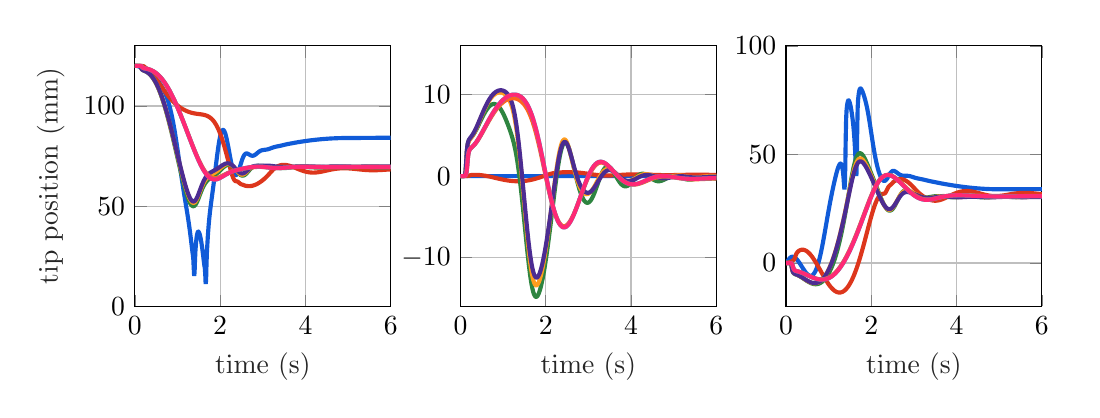
\begin{tikzpicture}

\begin{axis}[%
width=0.268\textwidth,
height=0.273\textwidth,
at={(0\textwidth,0\textwidth)},
scale only axis,
xmin=0,
xmax=6,
xlabel style={font=\color{white!15!black}},
xlabel={time (s)},
ymin=0,
ymax=130,
ylabel style={font=\color{white!15!black}},
ylabel={tip position (mm)},
axis background/.style={fill=white},
xmajorgrids,
ymajorgrids
]
\addplot [color=mycolor1, line width=1.5pt, forget plot]
  table[row sep=crcr]{%
0	119.999999824351\\
0.01	119.999761006601\\
0.02	119.996496846166\\
0.03	119.985718557839\\
0.04	119.964880088242\\
0.05	119.932615064138\\
0.06	119.889113056561\\
0.07	119.834971168929\\
0.08	119.771232053867\\
0.09	119.698883594988\\
0.1	119.618976052914\\
0.11	119.532387253545\\
0.12	119.439967448317\\
0.13	119.342396849961\\
0.14	119.240315312118\\
0.15	119.134221106263\\
0.16	119.024574745018\\
0.17	118.911723223345\\
0.18	118.795980138295\\
0.19	118.677568653634\\
0.2	118.556682579098\\
0.21	118.433443910826\\
0.22	118.307949170363\\
0.23	118.180238402931\\
0.24	118.050329515685\\
0.25	117.918196859364\\
0.26	117.783796300099\\
0.27	117.647050825152\\
0.28	117.507868093802\\
0.29	117.366132448605\\
0.3	117.221715873008\\
0.31	117.074474968299\\
0.32	116.924256085862\\
0.33	116.770896825164\\
0.34	116.614226581768\\
0.35	116.454071371469\\
0.36	116.290250163843\\
0.37	116.122582663887\\
0.38	115.950881994903\\
0.39	115.774964855416\\
0.4	115.594641170433\\
0.41	115.409725989712\\
0.42	115.220026140091\\
0.43	115.025353830792\\
0.44	114.825511278079\\
0.45	114.6203050157\\
0.46	114.409528667674\\
0.47	114.19297781361\\
0.48	113.970431366578\\
0.49	113.741666546228\\
0.5	113.506439320119\\
0.51	113.26449907836\\
0.52	113.01556848251\\
0.53	112.759357593083\\
0.54	112.495544085454\\
0.55	112.223785933177\\
0.56	111.943701974316\\
0.57	111.654883285866\\
0.58	111.356875160517\\
0.59	111.049186862381\\
0.6	110.731275262822\\
0.61	110.402552370005\\
0.62	110.062371175112\\
0.63	109.710030576761\\
0.64	109.344765679087\\
0.65	108.965750132387\\
0.66	108.572090469545\\
0.67	108.162824947057\\
0.68	107.736923681697\\
0.69	107.293284732\\
0.7	106.830740839743\\
0.71	106.348051858033\\
0.72	105.843919949\\
0.73	105.316978759632\\
0.74	104.765818020413\\
0.75	104.188969915192\\
0.76	103.584941931931\\
0.77	102.952203871275\\
0.78	102.289227928714\\
0.79	101.594479565251\\
0.8	100.866461926607\\
0.81	100.103710511407\\
0.82	99.3048447934397\\
0.83	98.4685642921724\\
0.84	97.5937084703769\\
0.85	96.6792513284613\\
0.86	95.7243693186971\\
0.87	94.7284338747264\\
0.88	93.6910840884815\\
0.89	92.6122140234625\\
0.9	91.4920477315701\\
0.91	90.331117496065\\
0.92	89.1303344501962\\
0.93	87.890955466455\\
0.94	86.6146466057379\\
0.95	85.3034288947525\\
0.96	83.9597403267121\\
0.97	82.5863444921697\\
0.98	81.1863913044906\\
0.99	79.7632824471517\\
1	78.3207349808177\\
1.01	76.862609158136\\
1.02	75.3929583165023\\
1.03	73.9158381233124\\
1.04	72.4353430744522\\
1.05	70.9554053657524\\
1.06	69.479821213836\\
1.07	68.0120522176315\\
1.08	66.5552500069188\\
1.09	65.112070980448\\
1.1	63.684707653561\\
1.11	62.2747260899165\\
1.12	60.8831103150038\\
1.13	59.5101283065856\\
1.14	58.1553925796929\\
1.15	56.8177565082787\\
1.16	55.4953906316062\\
1.17	54.1857073647971\\
1.18	52.885453351008\\
1.19	51.5906446741126\\
1.2	50.2966841931333\\
1.21	48.9983021544355\\
1.22	47.6896828069595\\
1.23	46.3644249125003\\
1.24	45.0156729663339\\
1.25	43.6361229825178\\
1.26	42.2181976301616\\
1.27	40.7541788096905\\
1.28	39.2365684654916\\
1.29	37.6586131046146\\
1.3	36.0153135263962\\
1.31	34.3052099274029\\
1.32	32.5336771995047\\
1.33	30.7191749438592\\
1.34	28.9054585390978\\
1.35	27.1868248823313\\
1.36	25.7641139588364\\
1.37	23.7389391233212\\
1.38	19.3350211852975\\
1.39	15.2538925166398\\
1.4	16.8089911140614\\
1.41	22.9813966198814\\
1.42	27.5893513818984\\
1.43	30.5631865870065\\
1.44	32.9554354592321\\
1.45	34.729879863386\\
1.46	35.9827973597344\\
1.47	36.770680025833\\
1.48	37.1772604175127\\
1.49	37.2542470310477\\
1.5	37.0599251420584\\
1.51	36.630939585206\\
1.52	36.0029125464571\\
1.53	35.1977061797354\\
1.54	34.2343819593173\\
1.55	33.1239310653069\\
1.56	31.8750304145053\\
1.57	30.4928159755338\\
1.58	28.9825110101808\\
1.59	27.3518917808935\\
1.6	25.6166950482456\\
1.61	23.8114558414142\\
1.62	22.0088089384839\\
1.63	20.3648618177955\\
1.64	19.2100048676026\\
1.65	16.2953511213352\\
1.66	11.2311103659594\\
1.67	13.0020331372442\\
1.68	21.322763212686\\
1.69	27.1282990723681\\
1.7	30.9973275550963\\
1.71	34.5741203246097\\
1.72	37.6709417498994\\
1.73	40.4085436565868\\
1.74	42.8025839962144\\
1.75	44.9553130469619\\
1.76	46.8967165638708\\
1.77	48.7010375052856\\
1.78	50.3948803576434\\
1.79	52.0286779966581\\
1.8	53.6206764859965\\
1.81	55.2032157379555\\
1.82	56.7861825055777\\
1.83	58.3885132293256\\
1.84	60.01279231464\\
1.85	61.6677659289419\\
1.86	63.3497434162017\\
1.87	65.059457884914\\
1.88	66.7879260403827\\
1.89	68.52963370126\\
1.9	70.2714955019447\\
1.91	72.0035460958136\\
1.92	73.7101393463483\\
1.93	75.3788277127393\\
1.94	76.9932010338721\\
1.95	78.5403341913678\\
1.96	80.0048223405911\\
1.97	81.3750163773188\\
1.98	82.6379178556449\\
1.99	83.7843841218846\\
2	84.8046513587129\\
2.01	85.6926903789515\\
2.02	86.4422318112658\\
2.03	87.0504431235982\\
2.04	87.514398435123\\
2.05	87.8342344105785\\
2.06	88.010030815908\\
2.07	88.0445498681167\\
2.08	87.9405145674255\\
2.09	87.7029801146142\\
2.1	87.3370029755592\\
2.11	86.8496563636592\\
2.12	86.2480473850792\\
2.13	85.5410019237123\\
2.14	84.7374355161328\\
2.15	83.847682250718\\
2.16	82.8821600529965\\
2.17	81.8523599528936\\
2.18	80.7698333087609\\
2.19	79.646904686426\\
2.2	78.4958652247314\\
2.21	77.3293881974067\\
2.22	76.1599852695569\\
2.23	75.0001922077615\\
2.24	73.8622163138894\\
2.25	72.7579819319192\\
2.26	71.6989145427131\\
2.27	70.6958684891569\\
2.28	69.7590266697855\\
2.29	68.8978022754576\\
2.3	68.1207645351111\\
2.31	67.4355463315514\\
2.32	66.8487516684116\\
2.33	66.3658806209972\\
2.34	65.9911905871545\\
2.35	65.7276394934708\\
2.36	65.5766766680308\\
2.37	65.5382340919874\\
2.38	65.6104568662753\\
2.39	65.7898243382961\\
2.4	66.0708340126949\\
2.41	66.4463093094803\\
2.42	66.9071469050241\\
2.43	67.4428044040451\\
2.44	68.041103714966\\
2.45	68.6889658892634\\
2.46	69.3723203912822\\
2.47	70.0769857479727\\
2.48	70.7885953630211\\
2.49	71.4935066475941\\
2.5	72.178697566217\\
2.51	72.8326017323247\\
2.52	73.4449118604577\\
2.53	74.0072539133297\\
2.54	74.5128800239664\\
2.55	74.9571340996971\\
2.56	75.3370592079007\\
2.57	75.6516818198894\\
2.58	75.9015521474145\\
2.59	76.0889040446052\\
2.6	76.2171638582587\\
2.61	76.2910014498474\\
2.62	76.3158828947013\\
2.63	76.2980955983085\\
2.64	76.2443219358967\\
2.65	76.161610851013\\
2.66	76.0570507527853\\
2.67	75.9377442659272\\
2.68	75.8105110751725\\
2.69	75.6818432203793\\
2.7	75.5576966456964\\
2.71	75.4435286962728\\
2.72	75.3440824875432\\
2.73	75.2634024485909\\
2.74	75.2047054979731\\
2.75	75.1704270753034\\
2.76	75.1621091742696\\
2.77	75.1805218574326\\
2.78	75.2255933797672\\
2.79	75.296481348591\\
2.8	75.3915909178757\\
2.81	75.5087553539008\\
2.82	75.6452200800347\\
2.83	75.7978721380976\\
2.84	75.963243032824\\
2.85	76.1377325178123\\
2.86	76.3176319933859\\
2.87	76.4993362283317\\
2.88	76.6793633067224\\
2.89	76.8545832719665\\
2.9	77.0221784597252\\
2.91	77.1798205144795\\
2.92	77.3256112010433\\
2.93	77.4582205297882\\
2.94	77.5768020788827\\
2.95	77.6810738961919\\
2.96	77.7711760150732\\
2.97	77.8477383285003\\
2.98	77.9117440308151\\
2.99	77.9645448093854\\
3	78.0077140455007\\
3.01	78.0430457060451\\
3.02	78.0724108082485\\
3.03	78.0977608873374\\
3.04	78.1209851748228\\
3.05	78.1438857391827\\
3.06	78.1680839907899\\
3.07	78.1950324612075\\
3.08	78.2259214073157\\
3.09	78.261704189547\\
3.1	78.3030314087901\\
3.11	78.3502959083633\\
3.12	78.4035892453636\\
3.13	78.4627668441313\\
3.14	78.5274227629503\\
3.15	78.5969574891257\\
3.16	78.6705779879866\\
3.17	78.7474134178356\\
3.18	78.826489546461\\
3.19	78.9068187850759\\
3.2	78.9873965991384\\
3.21	79.067291582938\\
3.22	79.145630366044\\
3.23	79.2216776561125\\
3.24	79.2948094848828\\
3.25	79.3645779625387\\
3.26	79.4306715868051\\
3.27	79.4929630875179\\
3.28	79.5514578643693\\
3.29	79.6063261406188\\
3.3	79.6578426487787\\
3.31	79.7064065547255\\
3.32	79.7524913845311\\
3.33	79.7966433060696\\
3.34	79.839393507196\\
3.35	79.8812894009318\\
3.36	79.9228417282843\\
3.37	79.9645324425972\\
3.38	80.0067649397883\\
3.39	80.0498824625666\\
3.4	80.0941268280084\\
3.41	80.1396650501282\\
3.42	80.1865576914593\\
3.43	80.2347935810503\\
3.44	80.2842665633455\\
3.45	80.3348168175165\\
3.46	80.3862135723966\\
3.47	80.4382003714997\\
3.48	80.4904806826947\\
3.49	80.5427638654243\\
3.5	80.5947505666758\\
3.51	80.646176215397\\
3.52	80.6967936283802\\
3.53	80.7464115227664\\
3.54	80.7948727161189\\
3.55	80.842086229659\\
3.56	80.8880006308934\\
3.57	80.9326295444866\\
3.58	80.9760208047223\\
3.59	81.0182763351319\\
3.6	81.05951863982\\
3.61	81.0999068384572\\
3.62	81.1396024860927\\
3.63	81.1787839381913\\
3.64	81.2176146873966\\
3.65	81.256254409671\\
3.66	81.2948351078373\\
3.67	81.3334698466427\\
3.68	81.372236066548\\
3.69	81.4111862156713\\
3.7	81.4503351396888\\
3.71	81.4896738365588\\
3.72	81.5291603342429\\
3.73	81.568735915289\\
3.74	81.6083183974979\\
3.75	81.6478196365807\\
3.76	81.6871398548199\\
3.77	81.7261850250984\\
3.78	81.7648609202483\\
3.79	81.8030890975276\\
3.8	81.8407996395257\\
3.81	81.8779451155642\\
3.82	81.9144907400809\\
3.83	81.9504265328052\\
3.84	81.9857543247636\\
3.85	82.0204986595586\\
3.86	82.0546921178108\\
3.87	82.0883842635341\\
3.88	82.1216263241668\\
3.89	82.1544791633113\\
3.9	82.1869981754254\\
3.91	82.2192412155069\\
3.92	82.2512544832593\\
3.93	82.2830811688312\\
3.94	82.3147488399477\\
3.95	82.3462792492158\\
3.96	82.3776773964318\\
3.97	82.4089425705775\\
3.98	82.4400589137975\\
3.99	82.4710074321803\\
4	82.5017576215125\\
4.01	82.5322799443577\\
4.02	82.5625379378999\\
4.03	82.5925005664572\\
4.04	82.6221342428461\\
4.05	82.651414525667\\
4.06	82.6803176202852\\
4.07	82.7088310697789\\
4.08	82.736944520015\\
4.09	82.7646592945555\\
4.1	82.7919784483496\\
4.11	82.8189153554284\\
4.12	82.8454832786317\\
4.13	82.8717241647932\\
4.14	82.8976778195749\\
4.15	82.9233557035116\\
4.16	82.948759901181\\
4.17	82.973900456914\\
4.18	82.9987791008816\\
4.19	83.0234000692363\\
4.2	83.0477605029629\\
4.21	83.0718598737741\\
4.22	83.0956913174115\\
4.23	83.1192509252202\\
4.24	83.1425294922472\\
4.25	83.1655216900392\\
4.26	83.1882180033994\\
4.27	83.2106136997601\\
4.28	83.232700786448\\
4.29	83.2544766945414\\
4.3	83.2759361539451\\
4.31	83.2970795537151\\
4.32	83.3179046976417\\
4.33	83.3384148609485\\
4.34	83.3586104525497\\
4.35	83.3784968342176\\
4.36	83.3980759593142\\
4.37	83.4173540529751\\
4.38	83.4363333116627\\
4.39	83.4550195449093\\
4.4	83.4734140131942\\
4.41	83.4915211113308\\
4.42	83.5093403912024\\
4.43	83.5268743303961\\
4.44	83.5441205477069\\
4.45	83.5610796577673\\
4.46	83.5777476489808\\
4.47	83.5941237920763\\
4.48	83.6102031241009\\
4.49	83.625984355918\\
4.5	83.6414623978441\\
4.51	83.6566362091654\\
4.52	83.6715013064621\\
4.53	83.6860575137569\\
4.54	83.7003014169483\\
4.55	83.7142339956048\\
4.56	83.7278530129497\\
4.57	83.7411605378249\\
4.58	83.7541552849809\\
4.59	83.766840058122\\
4.6	83.7792367767739\\
4.61	83.7913718412716\\
4.62	83.8032313300837\\
4.63	83.81479999738\\
4.64	83.8260647404473\\
4.65	83.8370153472394\\
4.66	83.8476398929946\\
4.67	83.8579318442698\\
4.68	83.8678834695624\\
4.69	83.8774931483073\\
4.7	83.8867581211507\\
4.71	83.8956815977717\\
4.72	83.9042650625394\\
4.73	83.9125152033218\\
4.74	83.9204359635296\\
4.75	83.9280354174981\\
4.76	83.9353177638927\\
4.77	83.9422902995029\\
4.78	83.9489555145284\\
4.79	83.9553182859186\\
4.8	83.9613781711632\\
4.81	83.9671368774433\\
4.82	83.9726139586504\\
4.83	83.9778323120415\\
4.84	83.9827721224253\\
4.85	83.9874104460724\\
4.86	83.9917264544875\\
4.87	83.9957029516345\\
4.88	83.999321921322\\
4.89	84.0025721476883\\
4.9	84.0054426658468\\
4.91	84.0079303461824\\
4.92	84.0100324033526\\
4.93	84.0117760838079\\
4.94	84.0131891100722\\
4.95	84.014267330396\\
4.96	84.0149963067401\\
4.97	84.015372545264\\
4.98	84.0153893539516\\
4.99	84.0150463620537\\
5	84.0143407403291\\
5.01	84.01328107037\\
5.02	84.0118849275556\\
5.03	84.0102062601699\\
5.04	84.0083590729177\\
5.05	84.0065091491664\\
5.06	84.0048272454695\\
5.07	84.0034850323588\\
5.08	84.0026359794321\\
5.09	84.0024089216415\\
5.1	84.0028911557214\\
5.11	84.004129911007\\
5.12	84.0061225194491\\
5.13	84.0088155198691\\
5.14	84.012112892147\\
5.15	84.0159102013202\\
5.16	84.0200807259451\\
5.17	84.0244838460464\\
5.18	84.0289693361664\\
5.19	84.0333816765265\\
5.2	84.0375709328946\\
5.21	84.041430504011\\
5.22	84.0448848901174\\
5.23	84.0479025052965\\
5.24	84.050483025023\\
5.25	84.0526449779125\\
5.26	84.0544255728667\\
5.27	84.0558895556475\\
5.28	84.0571147199799\\
5.29	84.0581927099006\\
5.3	84.0592148494099\\
5.31	84.060272217953\\
5.32	84.0614528011899\\
5.33	84.062825730434\\
5.34	84.0644192724852\\
5.35	84.0662526223484\\
5.36	84.0683264314441\\
5.37	84.0706221886685\\
5.38	84.073100383118\\
5.39	84.0757096804144\\
5.4	84.0783853447934\\
5.41	84.0810603441119\\
5.42	84.0836642676973\\
5.43	84.0861344357763\\
5.44	84.088414027859\\
5.45	84.0904617862464\\
5.46	84.0922483130711\\
5.47	84.0937634994039\\
5.48	84.0950105383213\\
5.49	84.0960109023854\\
5.5	84.0967962912425\\
5.51	84.0974116477469\\
5.52	84.097905812708\\
5.53	84.0983335346449\\
5.54	84.098745899923\\
5.55	84.0991924506404\\
5.56	84.0997124379979\\
5.57	84.1003380081611\\
5.58	84.101087028421\\
5.59	84.1019678979693\\
5.6	84.102974224212\\
5.61	84.1040913046531\\
5.62	84.1052931056538\\
5.63	84.1065479150818\\
5.64	84.1078189605705\\
5.65	84.1090678981426\\
5.66	84.1102577620415\\
5.67	84.1113554586235\\
5.68	84.1123341216931\\
5.69	84.1131753006148\\
5.7	84.1138680794803\\
5.71	84.1144125916486\\
5.72	84.1148151542187\\
5.73	84.1150926083153\\
5.74	84.1152657186952\\
5.75	84.1153625156717\\
5.76	84.1154111438166\\
5.77	84.1154427867141\\
5.78	84.1154845680096\\
5.79	84.1155626766276\\
5.8	84.1156958732753\\
5.81	84.115899302301\\
5.82	84.1161789602918\\
5.83	84.1165364283474\\
5.84	84.1169643857293\\
5.85	84.1174522089952\\
5.86	84.1179823419473\\
5.87	84.1185364603172\\
5.88	84.1190923143004\\
5.89	84.1196300163251\\
5.9	84.1201288979458\\
5.91	84.1205734689917\\
5.92	84.1209498886042\\
5.93	84.1212512596144\\
5.94	84.1214734699173\\
5.95	84.1216196799019\\
5.96	84.1216955010557\\
5.97	84.121712750905\\
5.98	84.121684132794\\
5.99	84.121626506635\\
6	84.1215553681989\\
};
\addplot [color=mycolor2, line width=1.5pt, forget plot]
  table[row sep=crcr]{%
0	119.999999824351\\
0.01	119.999991014243\\
0.02	119.999889390258\\
0.03	119.999535485152\\
0.04	119.998760133155\\
0.05	119.997450471406\\
0.06	119.99556425031\\
0.07	119.993096079894\\
0.08	119.990055528429\\
0.09	119.98644623745\\
0.1	119.982253658257\\
0.11	119.977431382967\\
0.12	119.971887316802\\
0.13	119.965461526466\\
0.14	119.957891956261\\
0.15	119.94875563848\\
0.16	119.937365880138\\
0.17	119.922586963459\\
0.18	119.902484155936\\
0.19	119.873638120626\\
0.2	119.829731469497\\
0.21	119.758547913388\\
0.22	119.632125824298\\
0.23	119.452120620277\\
0.24	119.270573392396\\
0.25	119.095892886942\\
0.26	118.920562687553\\
0.27	118.746461169925\\
0.28	118.570543557777\\
0.29	118.392160759183\\
0.3	118.209679864761\\
0.31	118.022587980869\\
0.32	117.829999347684\\
0.33	117.631735749018\\
0.34	117.427358145997\\
0.35	117.216896616682\\
0.36	117.000169437522\\
0.37	116.777321745889\\
0.38	116.548325206553\\
0.39	116.313387081317\\
0.4	116.072574452595\\
0.41	115.826130169693\\
0.42	115.574184376322\\
0.43	115.317002432537\\
0.44	115.054758839496\\
0.45	114.78773466506\\
0.46	114.516137199768\\
0.47	114.240259137618\\
0.48	113.960332719654\\
0.49	113.676659267367\\
0.5	113.389490110614\\
0.51	113.09913257395\\
0.52	112.80585229305\\
0.53	112.509960064564\\
0.54	112.211731663557\\
0.55	111.911478828516\\
0.56	111.60948501054\\
0.57	111.306058592954\\
0.58	111.001486811379\\
0.59	110.696072852177\\
0.6	110.390103762794\\
0.61	110.083874418412\\
0.62	109.777667105762\\
0.63	109.471770397994\\
0.64	109.1664621135\\
0.65	108.862018245917\\
0.66	108.558706578545\\
0.67	108.256789167357\\
0.68	107.956521512043\\
0.69	107.658149628815\\
0.7	107.361914359162\\
0.71	107.068043760437\\
0.72	106.776761809795\\
0.73	106.488276867413\\
0.74	106.202794074612\\
0.75	105.920500581063\\
0.76	105.641581000041\\
0.77	105.366200027394\\
0.78	105.094520377379\\
0.79	104.826683362733\\
0.8	104.562828790004\\
0.81	104.303074015903\\
0.82	104.04753533168\\
0.83	103.796305960134\\
0.84	103.549478504668\\
0.85	103.307122303239\\
0.86	103.069306559473\\
0.87	102.83607482727\\
0.88	102.607477186905\\
0.89	102.383533494471\\
0.9	102.164273905076\\
0.91	101.949692050917\\
0.92	101.739804492664\\
0.93	101.534588518467\\
0.94	101.33404143738\\
0.95	101.138123976582\\
0.96	100.946817692875\\
0.97	100.760070146318\\
0.98	100.577849798897\\
0.99	100.400094048429\\
1	100.226761139714\\
1.01	100.057781326615\\
1.02	99.89310553836\\
1.03	99.7326598417732\\
1.04	99.5763906584371\\
1.05	99.4242226538981\\
1.06	99.2761003388218\\
1.07	99.1319467080821\\
1.08	98.9917104416173\\
1.09	98.8553161418647\\
1.1	98.7227187184908\\
1.11	98.5938442765424\\
1.12	98.4686519894912\\
1.13	98.3470684151032\\
1.14	98.2290529506526\\
1.15	98.114547657328\\
1.16	98.0035216352424\\
1.17	97.8959219141119\\
1.18	97.7917191519593\\
1.19	97.6908668011858\\
1.2	97.5933372210961\\
1.21	97.4990873678469\\
1.22	97.4080925337894\\
1.23	97.3203127306488\\
1.24	97.2357236424887\\
1.25	97.1542862191628\\
1.26	97.0759717538918\\
1.27	97.000741358597\\
1.28	96.9285586274876\\
1.29	96.8593836065715\\
1.3	96.79316942329\\
1.31	96.7298654566163\\
1.32	96.6694063077948\\
1.33	96.6117499939083\\
1.34	96.556821004292\\
1.35	96.5045670346454\\
1.36	96.4548883790715\\
1.37	96.4077223947361\\
1.38	96.3629453595199\\
1.39	96.3204761292755\\
1.4	96.2801732360473\\
1.41	96.2419357925005\\
1.42	96.2055997456435\\
1.43	96.171044680851\\
1.44	96.1380791400128\\
1.45	96.1065620775658\\
1.46	96.0762730875188\\
1.47	96.0470491626083\\
1.48	96.018639790224\\
1.49	95.9908589167903\\
1.5	95.9634269013751\\
1.51	95.9361347685793\\
1.52	95.9086669617821\\
1.53	95.880787158924\\
1.54	95.8521491634785\\
1.55	95.8224859745339\\
1.56	95.791435702678\\
1.57	95.758691862113\\
1.58	95.7238710124843\\
1.59	95.6866348336439\\
1.6	95.6465712163688\\
1.61	95.603315551249\\
1.62	95.5564269391217\\
1.63	95.5055154878688\\
1.64	95.4501124995528\\
1.65	95.3898039977496\\
1.66	95.3240949364316\\
1.67	95.252548839512\\
1.68	95.1746462117448\\
1.69	95.0899300965844\\
1.7	94.9978589278362\\
1.71	94.8979544740531\\
1.72	94.7896532283889\\
1.73	94.6724676070452\\
1.74	94.5458230966126\\
1.75	94.4092192662874\\
1.76	94.2620689680611\\
1.77	94.1038644593425\\
1.78	93.9340114443585\\
1.79	93.7519998403197\\
1.8	93.5572339386607\\
1.81	93.3492071984468\\
1.82	93.1273290703737\\
1.83	92.8911033364538\\
1.84	92.6399521324794\\
1.85	92.3733973342591\\
1.86	92.0908823490876\\
1.87	91.7919560130574\\
1.88	91.4760927635306\\
1.89	91.1428784693131\\
1.9	90.7918296398155\\
1.91	90.4225805619408\\
1.92	90.0347022456864\\
1.93	89.6278901894456\\
1.94	89.2017838052031\\
1.95	88.7561540788304\\
1.96	88.2907242596794\\
1.97	87.8053566237652\\
1.98	87.2998752464595\\
1.99	86.7742510077556\\
2	86.2284326485994\\
2.01	85.6625105143896\\
2.02	85.0765762102495\\
2.03	84.4708587959191\\
2.04	83.8456180826774\\
2.05	83.2012478366063\\
2.06	82.5381923012224\\
2.07	81.8570342746568\\
2.08	81.1584203493573\\
2.09	80.4431441521623\\
2.1	79.712076420178\\
2.11	78.9662429644319\\
2.12	78.206756541475\\
2.13	77.434892069354\\
2.14	76.6520244738696\\
2.15	75.8596972807198\\
2.16	75.0595654043277\\
2.17	74.2534592966739\\
2.18	73.4433345618087\\
2.19	72.631333443249\\
2.2	71.8197454864447\\
2.21	71.0110724596337\\
2.22	70.2080106162675\\
2.23	69.4135357591039\\
2.24	68.6309345517931\\
2.25	67.8639538770113\\
2.26	67.1169505627966\\
2.27	66.3952078645816\\
2.28	65.7053319047871\\
2.29	65.0558229059067\\
2.3	64.4575351704136\\
2.31	63.9235870704571\\
2.32	63.4677603835671\\
2.33	63.1012375151511\\
2.34	62.8284861616922\\
2.35	62.644547983156\\
2.36	62.534616359027\\
2.37	62.4760512955619\\
2.38	62.4420103035562\\
2.39	62.4062851268204\\
2.4	62.3479285153312\\
2.41	62.254604652177\\
2.42	62.1234829898326\\
2.43	61.9601941609231\\
2.44	61.7762579741385\\
2.45	61.5861560820988\\
2.46	61.4041584674015\\
2.47	61.2416516064435\\
2.48	61.1050462374021\\
2.49	60.9950317324375\\
2.5	60.9070807035666\\
2.51	60.8333627998149\\
2.52	60.7651282272565\\
2.53	60.6951960243614\\
2.54	60.6195625400608\\
2.55	60.5380574382983\\
2.56	60.4536422153857\\
2.57	60.3711010781691\\
2.58	60.2953804072076\\
2.59	60.2302872243378\\
2.6	60.1775443261811\\
2.61	60.1367360517263\\
2.62	60.1057569128657\\
2.63	60.0818222252687\\
2.64	60.0624191466328\\
2.65	60.0460724293189\\
2.66	60.0324979972274\\
2.67	60.0225616257068\\
2.68	60.0177635837788\\
2.69	60.0196731677838\\
2.7	60.029421261722\\
2.71	60.0474079938301\\
2.72	60.0733538541455\\
2.73	60.1064633423939\\
2.74	60.1458303949559\\
2.75	60.1906590219005\\
2.76	60.240544861674\\
2.77	60.2954235157749\\
2.78	60.3555702957541\\
2.79	60.4213449396089\\
2.8	60.4931290012296\\
2.81	60.5710993990504\\
2.82	60.655234163101\\
2.83	60.7452810780974\\
2.84	60.840946082873\\
2.85	60.9418737544041\\
2.86	61.047819153412\\
2.87	61.1585800253725\\
2.88	61.2740940284376\\
2.89	61.3943205644766\\
2.9	61.5192891128679\\
2.91	61.6489887754099\\
2.92	61.7834229280178\\
2.93	61.9225296771411\\
2.94	62.0662621037112\\
2.95	62.214523630515\\
2.96	62.3672606616835\\
2.97	62.5243942864785\\
2.98	62.6859179988244\\
2.99	62.8518079968958\\
3	63.0220924601612\\
3.01	63.1967772438258\\
3.02	63.3759333394589\\
3.03	63.5595959115154\\
3.04	63.7478503595305\\
3.05	63.9407416835083\\
3.06	64.1383455780229\\
3.07	64.3406662953179\\
3.08	64.5477151740312\\
3.09	64.7594089574876\\
3.1	64.9756433532311\\
3.11	65.1961912312517\\
3.12	65.4207692657188\\
3.13	65.6489444539489\\
3.14	65.8802174667792\\
3.15	66.1139288857918\\
3.16	66.3493381972315\\
3.17	66.5855535975393\\
3.18	66.8216241191684\\
3.19	67.0564849316166\\
3.2	67.2890583334487\\
3.21	67.5182119408859\\
3.22	67.7428616710948\\
3.23	67.9619351067715\\
3.24	68.174471688515\\
3.25	68.3795662119303\\
3.26	68.5764841734333\\
3.27	68.7645688231607\\
3.28	68.9433584365053\\
3.29	69.1124844111951\\
3.3	69.271761648516\\
3.31	69.4210576480743\\
3.32	69.5603945478087\\
3.33	69.6898424705855\\
3.34	69.8095876156189\\
3.35	69.9198298185797\\
3.36	70.0208503520139\\
3.37	70.1129027338157\\
3.38	70.1963131914935\\
3.39	70.2713489320793\\
3.4	70.3383139765104\\
3.41	70.3974478430752\\
3.42	70.4490311133011\\
3.43	70.49327127563\\
3.44	70.5304216708848\\
3.45	70.5606644605543\\
3.46	70.5842246981071\\
3.47	70.6012731047343\\
3.48	70.6120186097272\\
3.49	70.6166310738585\\
3.5	70.6153059166831\\
3.51	70.6082318461\\
3.52	70.5955843519204\\
3.53	70.5775738816009\\
3.54	70.5543710709503\\
3.55	70.5261958680561\\
3.56	70.4932253606245\\
3.57	70.4556887579617\\
3.58	70.4137634327165\\
3.59	70.3676881637239\\
3.6	70.3176391509763\\
3.61	70.2638494658541\\
3.62	70.2064990569033\\
3.63	70.1458156823993\\
3.64	70.0819781386178\\
3.65	70.015213216771\\
3.66	69.9456939665844\\
3.67	69.8736463600372\\
3.68	69.7992380869771\\
3.69	69.7226944426901\\
3.7	69.6441786182201\\
3.71	69.5639154699675\\
3.72	69.4820645086297\\
3.73	69.398850178377\\
3.74	69.3144288088151\\
3.75	69.2290240649318\\
3.76	69.1427891590811\\
3.77	69.0559461789348\\
3.78	68.9686448633715\\
3.79	68.8811045622248\\
3.8	68.7934708613947\\
3.81	68.7059589720602\\
3.82	68.618709450233\\
3.83	68.53193185578\\
3.84	68.4457607559516\\
3.85	68.3603985394437\\
3.86	68.2759728281281\\
3.87	68.1926773816941\\
3.88	68.1106319715586\\
3.89	68.0300203692083\\
3.9	67.9509536638917\\
3.91	67.8736043928131\\
3.92	67.7980742108643\\
3.93	67.7245232921399\\
3.94	67.6530431856881\\
3.95	67.5837806935636\\
3.96	67.5168166709604\\
3.97	67.4522836642544\\
3.98	67.3902513366055\\
3.99	67.3308372286013\\
4	67.2740994115522\\
4.01	67.2201398124142\\
4.02	67.1690046170367\\
4.03	67.1207796795395\\
4.04	67.0754943536191\\
4.05	67.0332244477558\\
4.06	66.9939844632743\\
4.07	66.9578368444671\\
4.08	66.9247842164805\\
4.09	66.8948750037629\\
4.1	66.8680954579823\\
4.11	66.8444782164148\\
4.12	66.8239959358318\\
4.13	66.8066631420567\\
4.14	66.7924395825526\\
4.15	66.7813269656948\\
4.16	66.7732751519146\\
4.17	66.7682702971006\\
4.18	66.7662526118617\\
4.19	66.7671930654816\\
4.2	66.7710262074505\\
4.21	66.7777053390075\\
4.22	66.7871621455529\\
4.23	66.7993276026337\\
4.24	66.8141328761375\\
4.25	66.8314864384703\\
4.26	66.8513167169534\\
4.27	66.8735184135005\\
4.28	66.8980179307098\\
4.29	66.9247006811034\\
4.3	66.9534892067528\\
4.31	66.9842584563743\\
4.32	67.0169238857711\\
4.33	67.0513577557331\\
4.34	67.0874716475665\\
4.35	67.1251349171016\\
4.36	67.1642585819828\\
4.37	67.2047069536165\\
4.38	67.2463917854289\\
4.39	67.2891737380433\\
4.4	67.332966313641\\
4.41	67.3776281155878\\
4.42	67.4230754289754\\
4.43	67.4691664134892\\
4.44	67.5158211239346\\
4.45	67.5628988177836\\
4.46	67.6103241882748\\
4.47	67.6579589958128\\
4.48	67.7057332798023\\
4.49	67.7535125395551\\
4.5	67.8012326939997\\
4.51	67.8487640421109\\
4.52	67.8960487498293\\
4.53	67.9429628121473\\
4.54	67.9894548634674\\
4.55	68.0354073441366\\
4.56	68.0807754544798\\
4.57	68.1254486990626\\
4.58	68.1693888364101\\
4.59	68.2124929359508\\
4.6	68.2547292154073\\
4.61	68.2960026993505\\
4.62	68.3362878844632\\
4.63	68.3754980356665\\
4.64	68.4136136755128\\
4.65	68.4505564944312\\
4.66	68.4863127237052\\
4.67	68.5208125708485\\
4.68	68.5540476051236\\
4.69	68.5859565577494\\
4.7	68.6165359238556\\
4.71	68.6457328905821\\
4.72	68.6735484389259\\
4.73	68.6999380814134\\
4.74	68.7249068307391\\
4.75	68.7484138440626\\
4.76	68.7704737436526\\
4.77	68.7910512121444\\
4.78	68.8101668540018\\
4.79	68.8277933239703\\
4.8	68.8439564173182\\
4.81	68.8586318160294\\
4.82	68.8718481132328\\
4.83	68.8835822328308\\
4.84	68.893868224394\\
4.85	68.9026909313403\\
4.86	68.9100853896975\\
4.87	68.9160471688783\\
4.88	68.9206076742636\\
4.89	68.9237733614443\\
4.9	68.9255732930998\\
4.91	68.9260225476212\\
4.92	68.9251462098267\\
4.93	68.9229694899718\\
4.94	68.9195115923975\\
4.95	68.9148101072046\\
4.96	68.9088784406531\\
4.97	68.9017618860993\\
4.98	68.8934734391236\\
4.99	68.8840655413847\\
5	68.8735506862255\\
5.01	68.8619895040063\\
5.02	68.8493967945998\\
5.03	68.8358381663595\\
5.04	68.8213349655769\\
5.05	68.8059594766664\\
5.06	68.7897340099153\\
5.07	68.7727355477038\\
5.08	68.7549841963492\\
5.09	68.7365548344142\\
5.1	68.7174701482186\\
5.11	68.6978030025026\\
5.12	68.6775773082687\\
5.13	68.6568663080758\\
5.14	68.6356922048798\\
5.15	68.6141291831796\\
5.16	68.592198514371\\
5.17	68.56997563143\\
5.18	68.5474815943066\\
5.19	68.5247930966385\\
5.2	68.5019313517597\\
5.21	68.4789739408536\\
5.22	68.4559422159625\\
5.23	68.432913948247\\
5.24	68.4099103406396\\
5.25	68.3870084751798\\
5.26	68.36422899433\\
5.27	68.3416473793276\\
5.28	68.3192833053732\\
5.29	68.2972098154017\\
5.3	68.2754452899305\\
5.31	68.2540596193451\\
5.32	68.2330696611298\\
5.33	68.2125415627691\\
5.34	68.1924905108698\\
5.35	68.1729784169201\\
5.36	68.1540186950464\\
5.37	68.1356727029492\\
5.38	68.1179466812812\\
5.39	68.100899545902\\
5.4	68.0845324049883\\
5.41	68.0688987964556\\
5.42	68.0539985749585\\
5.43	68.0398793293464\\
5.44	68.026535335554\\
5.45	68.0140138535607\\
5.46	68.0023056104412\\
5.47	67.9914538159594\\
5.48	67.9814481258428\\
5.49	67.9723231529762\\
5.5	67.964067799236\\
5.51	67.956707734423\\
5.52	67.9502311909773\\
5.53	67.9446579565933\\
5.54	67.9399720919519\\
5.55	67.9361862576654\\
5.56	67.9332825323362\\
5.57	67.9312644727214\\
5.58	67.9301158221433\\
5.59	67.9298312550083\\
5.6	67.9303964064977\\
5.61	67.9317977984955\\
5.62	67.9340229197029\\
5.63	67.9370489341108\\
5.64	67.9408650875798\\
5.65	67.9454414716547\\
5.66	67.9507690670935\\
5.67	67.9568103447718\\
5.68	67.9635579155508\\
5.69	67.9709672716591\\
5.7	67.9790288330524\\
5.71	67.9876965694074\\
5.72	67.99695939955\\
5.73	68.0067696215038\\
5.74	68.0171167239211\\
5.75	68.0279489081379\\
5.76	68.0392564277618\\
5.77	68.0509839140819\\
5.78	68.0631224873556\\
5.79	68.0756138959335\\
5.8	68.0884502721642\\
5.81	68.1015712115576\\
5.82	68.1149700045929\\
5.83	68.1285848121902\\
5.84	68.1424101923967\\
5.85	68.1563835453491\\
5.86	68.1705007531021\\
5.87	68.184699072751\\
5.88	68.1989757155504\\
5.89	68.213268360455\\
5.9	68.2275755141747\\
5.91	68.2418357994304\\
5.92	68.2560489606391\\
5.93	68.2701550527625\\
5.94	68.2841549881963\\
5.95	68.2979907145693\\
5.96	68.3116642373292\\
5.97	68.3251198295373\\
5.98	68.3383605114872\\
5.99	68.3513332834609\\
6	68.3640420980248\\
};
\addplot [color=mycolor3, line width=1.5pt, forget plot]
  table[row sep=crcr]{%
0	119.999999824351\\
0.01	119.999999823849\\
0.02	119.99999982016\\
0.03	119.999999792279\\
0.04	119.999999603748\\
0.05	119.999998628326\\
0.06	119.999994296716\\
0.07	119.99997572178\\
0.08	119.999892691566\\
0.09	119.999492399102\\
0.1	119.997398205762\\
0.11	119.981815462772\\
0.12	119.89815396777\\
0.13	119.648152329234\\
0.14	119.225177632991\\
0.15	118.780571852625\\
0.16	118.435002635377\\
0.17	118.184066668593\\
0.18	117.999634077072\\
0.19	117.859559905154\\
0.2	117.746123993776\\
0.21	117.647663755165\\
0.22	117.555918621618\\
0.23	117.465598571318\\
0.24	117.372908038536\\
0.25	117.275423893\\
0.26	117.171273410429\\
0.27	117.059245989296\\
0.28	116.938291283199\\
0.29	116.80771173568\\
0.3	116.666820293407\\
0.31	116.515145019628\\
0.32	116.352172701358\\
0.33	116.17753992529\\
0.34	115.990828897499\\
0.35	115.791737382328\\
0.36	115.57990979986\\
0.37	115.355086009338\\
0.38	115.116958289631\\
0.39	114.865300944824\\
0.4	114.599847209012\\
0.41	114.320403354038\\
0.42	114.026740520941\\
0.43	113.718696303003\\
0.44	113.39607771947\\
0.45	113.058753088018\\
0.46	112.706564738964\\
0.47	112.339411529575\\
0.48	111.957171138423\\
0.49	111.559773228602\\
0.5	111.147130664132\\
0.51	110.719204273602\\
0.52	110.275942027403\\
0.53	109.817336252152\\
0.54	109.34336994505\\
0.55	108.85406716544\\
0.56	108.349445788037\\
0.57	107.829561691911\\
0.58	107.294467360348\\
0.59	106.744250399051\\
0.6	106.178997479915\\
0.61	105.598827646155\\
0.62	105.003861172941\\
0.63	104.394248055064\\
0.64	103.770141421022\\
0.65	103.131721547081\\
0.66	102.479173514389\\
0.67	101.812707050597\\
0.68	101.132537341932\\
0.69	100.438903571432\\
0.7	99.7320500363449\\
0.71	99.0122450055057\\
0.72	98.2797601785442\\
0.73	97.5348910657643\\
0.74	96.7779359300982\\
0.75	96.0092158675055\\
0.76	95.2290553119858\\
0.77	94.4377998961731\\
0.78	93.6357992412522\\
0.79	92.823422660152\\
0.8	92.0010441402847\\
0.81	91.1690560282983\\
0.82	90.3278560979687\\
0.83	89.4778593579645\\
0.84	88.619487099992\\
0.85	87.7531769700782\\
0.86	86.8793738944855\\
0.87	85.9985385556746\\
0.88	85.1111400943892\\
0.89	84.2176631340292\\
0.9	83.3186021566894\\
0.91	82.414467224059\\
0.92	81.5057799231747\\
0.93	80.5930779379353\\
0.94	79.6769124568998\\
0.95	78.7578517567091\\
0.96	77.8364799593206\\
0.97	76.9133997964811\\
0.98	75.9892325971152\\
0.99	75.0646204096738\\
1	74.1402270916359\\
1.01	73.216738568695\\
1.02	72.2948692146272\\
1.03	71.3753562379476\\
1.04	70.4589734625252\\
1.05	69.5465172958856\\
1.06	68.6388284453076\\
1.07	67.7367724694264\\
1.08	66.8412661495421\\
1.09	65.9532565644843\\
1.1	65.0737480651191\\
1.11	64.2037814766208\\
1.12	63.3444614587621\\
1.13	62.4969359677818\\
1.14	61.6624238708928\\
1.15	60.8421947703259\\
1.16	60.037596806297\\
1.17	59.2500369100186\\
1.18	58.4810087924473\\
1.19	57.7320735947909\\
1.2	57.0048863553233\\
1.21	56.3011804837791\\
1.22	55.6227967383464\\
1.23	54.9716577280868\\
1.24	54.3497962502536\\
1.25	53.7593335523021\\
1.26	53.202503044241\\
1.27	52.6816205057491\\
1.28	52.1991009190681\\
1.29	51.7574122121614\\
1.3	51.3590953580861\\
1.31	51.0066707995272\\
1.32	50.7026702380949\\
1.33	50.4494924977539\\
1.34	50.2494311076526\\
1.35	50.1044959986815\\
1.36	50.0164280746365\\
1.37	49.9864983422979\\
1.38	50.015523414641\\
1.39	50.1036596929006\\
1.4	50.2504431184724\\
1.41	50.4546034367809\\
1.42	50.7141499888445\\
1.43	51.0262483025054\\
1.44	51.3873431099856\\
1.45	51.7931242584356\\
1.46	52.2386969168658\\
1.47	52.7186146923828\\
1.48	53.2270983388553\\
1.49	53.7581021371229\\
1.5	54.3055547464764\\
1.51	54.8634295731772\\
1.52	55.4259721481638\\
1.53	55.9877479958055\\
1.54	56.5438268911362\\
1.55	57.0897911805644\\
1.56	57.6218598229947\\
1.57	58.1368528379402\\
1.58	58.6322544006542\\
1.59	59.106133038058\\
1.6	59.5571654885955\\
1.61	59.9845240951982\\
1.62	60.3878714468617\\
1.63	60.767244739106\\
1.64	61.1230282831834\\
1.65	61.4558616503098\\
1.66	61.7666106695821\\
1.67	62.0562837664917\\
1.68	62.3260166442761\\
1.69	62.5770209539934\\
1.7	62.8105741158074\\
1.71	63.0279900730129\\
1.72	63.2306157544909\\
1.73	63.4198256897045\\
1.74	63.5969989222251\\
1.75	63.7635375727856\\
1.76	63.9208420364081\\
1.77	64.0703322682206\\
1.78	64.2133945950707\\
1.79	64.3514404122418\\
1.8	64.485817907999\\
1.81	64.6178892921237\\
1.82	64.7489227789697\\
1.83	64.8801693797351\\
1.84	65.0127648471109\\
1.85	65.1477947009425\\
1.86	65.2862099532619\\
1.87	65.4288793380332\\
1.88	65.5765077278507\\
1.89	65.7297034680598\\
1.9	65.8888933943768\\
1.91	66.0543972882005\\
1.92	66.2263430277374\\
1.93	66.404749605581\\
1.94	66.5894421132691\\
1.95	66.7801430826983\\
1.96	66.976386948142\\
1.97	67.1776191048837\\
1.98	67.383109284631\\
1.99	67.5920575541778\\
2	67.8035059623882\\
2.01	68.0164506158829\\
2.02	68.2297509872217\\
2.03	68.4422471725674\\
2.04	68.6526663586147\\
2.05	68.8597430131321\\
2.06	69.0621237230357\\
2.07	69.258493868446\\
2.08	69.447475232989\\
2.09	69.6277535605851\\
2.1	69.7979758232369\\
2.11	69.9568793496998\\
2.12	70.1031855704684\\
2.13	70.2357303026678\\
2.14	70.3533549111215\\
2.15	70.4550368639698\\
2.16	70.5397808418356\\
2.17	70.6067470375154\\
2.18	70.6551367843998\\
2.19	70.6843238077379\\
2.2	70.6937430480758\\
2.21	70.6830165122351\\
2.22	70.6518429082477\\
2.23	70.6001206732221\\
2.24	70.5278397427455\\
2.25	70.4352001451695\\
2.26	70.3225071719353\\
2.27	70.190284088364\\
2.28	70.0391718257703\\
2.29	69.87003414713\\
2.3	69.6838628554242\\
2.31	69.4818734849864\\
2.32	69.26541682982\\
2.33	69.0360629361455\\
2.34	68.7955194962304\\
2.35	68.5457016202043\\
2.36	68.2886573375209\\
2.37	68.0266203778397\\
2.38	67.7619427278369\\
2.39	67.4971275335932\\
2.4	67.234768475608\\
2.41	66.9775600370786\\
2.42	66.7282483639856\\
2.43	66.4896069526451\\
2.44	66.2643863674144\\
2.45	66.055286998734\\
2.46	65.864922253468\\
2.47	65.6957423601187\\
2.48	65.5500212903488\\
2.49	65.4297549321301\\
2.5	65.3366758623165\\
2.51	65.2721185266139\\
2.52	65.2370827881502\\
2.53	65.2320777559499\\
2.54	65.2572134349127\\
2.55	65.3120781955634\\
2.56	65.3958388384575\\
2.57	65.5071506064587\\
2.58	65.6442673802521\\
2.59	65.8049981254991\\
2.6	65.9868535223528\\
2.61	66.1870050619732\\
2.62	66.4024550065973\\
2.63	66.6300095882595\\
2.64	66.8664556187381\\
2.65	67.1085367388899\\
2.66	67.3531219278169\\
2.67	67.5971763179121\\
2.68	67.8379089756375\\
2.69	68.072732907422\\
2.7	68.2993842797654\\
2.71	68.5158703586955\\
2.72	68.7205576987296\\
2.73	68.9121104049862\\
2.74	69.089551995276\\
2.75	69.2521888852553\\
2.76	69.3996551951447\\
2.77	69.5318372041112\\
2.78	69.6489169515225\\
2.79	69.751254636385\\
2.8	69.839438972845\\
2.81	69.9141830180285\\
2.82	69.9763760356088\\
2.83	70.0269774114732\\
2.84	70.0670496997952\\
2.85	70.0976516168858\\
2.86	70.1199048080722\\
2.87	70.1348996740003\\
2.88	70.1437080475944\\
2.89	70.1473470698953\\
2.9	70.1467632709777\\
2.91	70.1428367082805\\
2.92	70.1363365046883\\
2.93	70.127963688569\\
2.94	70.1182952938011\\
2.95	70.1078292658205\\
2.96	70.0969211580897\\
2.97	70.0858681816805\\
2.98	70.0748293411173\\
2.99	70.0639244947337\\
3	70.0531453513305\\
3.01	70.0424649592531\\
3.02	70.0317553384288\\
3.03	70.0208872095669\\
3.04	70.0096564623256\\
3.05	69.9978803779782\\
3.06	69.985322321208\\
3.07	69.9717908692986\\
3.08	69.9570586538679\\
3.09	69.9409632877644\\
3.1	69.9233206208959\\
3.11	69.904025721314\\
3.12	69.882961411562\\
3.13	69.860097766764\\
3.14	69.8353972121328\\
3.15	69.8089112447691\\
3.16	69.7806837126048\\
3.17	69.750843693842\\
3.18	69.7195088220634\\
3.19	69.6868734535116\\
3.2	69.6531140352151\\
3.21	69.6184718521158\\
3.22	69.5831624484904\\
3.23	69.5474569464667\\
3.24	69.5115821160961\\
3.25	69.4758150244052\\
3.26	69.4403725802207\\
3.27	69.4055196218038\\
3.28	69.3714502175714\\
3.29	69.3383966959961\\
3.3	69.3065198154738\\
3.31	69.2760100867138\\
3.32	69.2469909757449\\
3.33	69.2195948232749\\
3.34	69.1938965037334\\
3.35	69.1699865438216\\
3.36	69.1479034612263\\
3.37	69.1276967612024\\
3.38	69.1093787201858\\
3.39	69.0929660381493\\
3.4	69.078456257082\\
3.41	69.065845522339\\
3.42	69.0551279152873\\
3.43	69.0462896961382\\
3.44	69.0393324396778\\
3.45	69.0342411563669\\
3.46	69.0310304154551\\
3.47	69.0296888598637\\
3.48	69.0302417754411\\
3.49	69.0326852899669\\
3.5	69.0370512874258\\
3.51	69.0433372443878\\
3.52	69.0515745605425\\
3.53	69.0617514746265\\
3.54	69.0738878143739\\
3.55	69.0879515941113\\
3.56	69.1039387253563\\
3.57	69.121786153137\\
3.58	69.1414547493143\\
3.59	69.1628417067067\\
3.6	69.1858648967369\\
3.61	69.2103769647272\\
3.62	69.2362494449587\\
3.63	69.2632906571459\\
3.64	69.2913278599743\\
3.65	69.3201306704105\\
3.66	69.3494895342133\\
3.67	69.3791460027051\\
3.68	69.4088658375276\\
3.69	69.4383771055926\\
3.7	69.4674363401316\\
3.71	69.4957750704369\\
3.72	69.5231596448191\\
3.73	69.5493399113915\\
3.74	69.5741078526949\\
3.75	69.5972493220974\\
3.76	69.6185950778391\\
3.77	69.6379817729602\\
3.78	69.6552896525693\\
3.79	69.6704149425883\\
3.8	69.6832938004342\\
3.81	69.6938856696474\\
3.82	69.7021839842579\\
3.83	69.7082098191069\\
3.84	69.7120102819799\\
3.85	69.7136616774476\\
3.86	69.7132568789703\\
3.87	69.710917129981\\
3.88	69.7067699314514\\
3.89	69.7009685435243\\
3.9	69.6936620898131\\
3.91	69.6850217671815\\
3.92	69.6752047794935\\
3.93	69.6643862460408\\
3.94	69.6527187952978\\
3.95	69.6403691814783\\
3.96	69.6274749429389\\
3.97	69.6141846587698\\
3.98	69.6006130738495\\
3.99	69.5868839997209\\
4	69.5730850579547\\
4.01	69.5593122312845\\
4.02	69.5456251601344\\
4.03	69.5320923846406\\
4.04	69.5187479200255\\
4.05	69.5056362755948\\
4.06	69.4927686081099\\
4.07	69.4801729098547\\
4.08	69.4678468317672\\
4.09	69.4558075434666\\
4.1	69.4440475849085\\
4.11	69.4325803405797\\
4.12	69.4214000989305\\
4.13	69.4105246196604\\
4.14	69.3999551644517\\
4.15	69.3897190416831\\
4.16	69.3798297150691\\
4.17	69.3703266887976\\
4.18	69.3612399280699\\
4.19	69.3526203060488\\
4.2	69.3445133283245\\
4.21	69.336980752796\\
4.22	69.3300799218005\\
4.23	69.3238799464961\\
4.24	69.3184445041834\\
4.25	69.3138439850118\\
4.26	69.3101414832341\\
4.27	69.3074013711541\\
4.28	69.3056784881892\\
4.29	69.3050236449037\\
4.3	69.3054759927228\\
4.31	69.3070662364776\\
4.32	69.3098110067471\\
4.33	69.3137153704174\\
4.34	69.3187691561885\\
4.35	69.3249483544652\\
4.36	69.3322143240343\\
4.37	69.3405134208307\\
4.38	69.349779032629\\
4.39	69.3599300462136\\
4.4	69.3708749619598\\
4.41	69.382509779808\\
4.42	69.3947234136487\\
4.43	69.4073954819775\\
4.44	69.420402247196\\
4.45	69.433614696932\\
4.46	69.446904286653\\
4.47	69.460141597723\\
4.48	69.4732012588924\\
4.49	69.4859613728448\\
4.5	69.4983071238388\\
4.51	69.5101310798065\\
4.52	69.5213351472251\\
4.53	69.5318317833566\\
4.54	69.5415441214597\\
4.55	69.5504077711762\\
4.56	69.5583699656994\\
4.57	69.5653910213906\\
4.58	69.5714430759537\\
4.59	69.5765110198137\\
4.6	69.5805903996892\\
4.61	69.5836886518639\\
4.62	69.5858220674689\\
4.63	69.5870172592412\\
4.64	69.5873074883732\\
4.65	69.5867343123635\\
4.66	69.5853435573305\\
4.67	69.5831871183455\\
4.68	69.5803188461983\\
4.69	69.576796406776\\
4.7	69.5726773619952\\
4.71	69.5680210998285\\
4.72	69.5628852456337\\
4.73	69.5573275920508\\
4.74	69.551403016607\\
4.75	69.5451653602441\\
4.76	69.5386651069599\\
4.77	69.5319506856523\\
4.78	69.5250673817156\\
4.79	69.5180576522063\\
4.8	69.51096148471\\
4.81	69.5038160770412\\
4.82	69.4966568955468\\
4.83	69.489516907449\\
4.84	69.4824282969171\\
4.85	69.4754211668458\\
4.86	69.4685258178555\\
4.87	69.4617708806548\\
4.88	69.4551860467424\\
4.89	69.4487996167946\\
4.9	69.4426415722079\\
4.91	69.4367405522626\\
4.92	69.4311271653057\\
4.93	69.4258304381737\\
4.94	69.4208809387805\\
4.95	69.4163077912303\\
4.96	69.4121405792906\\
4.97	69.4084073613499\\
4.98	69.4051354705769\\
4.99	69.402349764737\\
5	69.4000734156107\\
5.01	69.3983260748223\\
5.02	69.3971248327269\\
5.03	69.3964826971254\\
5.04	69.3964092201639\\
5.05	69.3969087930349\\
5.06	69.3979809076685\\
5.07	69.3996196156516\\
5.08	69.4018130809007\\
5.09	69.4045442136686\\
5.1	69.4077898038723\\
5.11	69.4115217856212\\
5.12	69.4157061191843\\
5.13	69.4203048079241\\
5.14	69.4252743868274\\
5.15	69.4305687497444\\
5.16	69.4361371265195\\
5.17	69.441927734265\\
5.18	69.4478851357787\\
5.19	69.4539546915572\\
5.2	69.4600792130683\\
5.21	69.46620415931\\
5.22	69.4722735297894\\
5.23	69.4782357216824\\
5.24	69.4840386465615\\
5.25	69.4896361422867\\
5.26	69.4949823411104\\
5.27	69.5000385145594\\
5.28	69.5047667645712\\
5.29	69.5091371696579\\
5.3	69.513120911348\\
5.31	69.5166975854102\\
5.32	69.5198479097705\\
5.33	69.5225610648969\\
5.34	69.5248271540495\\
5.35	69.5266439971273\\
5.36	69.5280108875956\\
5.37	69.5289334253684\\
5.38	69.5294190278597\\
5.39	69.5294801603141\\
5.4	69.5291305662133\\
5.41	69.5283881912343\\
5.42	69.527271770739\\
5.43	69.5258032737316\\
5.44	69.5240050472166\\
5.45	69.5219014125591\\
5.46	69.519516950725\\
5.47	69.5168773364718\\
5.48	69.5140083257824\\
5.49	69.5109359576233\\
5.5	69.5076863478252\\
5.51	69.5042851948611\\
5.52	69.5007584014581\\
5.53	69.4971308683064\\
5.54	69.4934279283258\\
5.55	69.4896734303269\\
5.56	69.4858919451673\\
5.57	69.4821061575539\\
5.58	69.478339782913\\
5.59	69.474614301515\\
5.6	69.4709525095048\\
5.61	69.4673746454247\\
5.62	69.4639024882357\\
5.63	69.4605549418603\\
5.64	69.4573525866642\\
5.65	69.4543128023821\\
5.66	69.4514546767179\\
5.67	69.4487937603426\\
5.68	69.4463472361782\\
5.69	69.444128411365\\
5.7	69.4421520525687\\
5.71	69.4404287692518\\
5.72	69.438970413859\\
5.73	69.4377843999348\\
5.74	69.4368788159817\\
5.75	69.4362572810743\\
5.76	69.4359234503015\\
5.77	69.4358771197661\\
5.78	69.4361171617854\\
5.79	69.4366393590683\\
5.8	69.4374379111087\\
5.81	69.4385041159648\\
5.82	69.4398275584904\\
5.83	69.4413952383713\\
5.84	69.4431923806913\\
5.85	69.4452020969231\\
5.86	69.4474057513317\\
5.87	69.4497832030555\\
5.88	69.4523126744642\\
5.89	69.4549716008637\\
5.9	69.457735958416\\
5.91	69.4605817275806\\
5.92	69.4634836518571\\
5.93	69.4664173016543\\
5.94	69.4693572509021\\
5.95	69.4722797102581\\
5.96	69.4751601260567\\
5.97	69.4779763361772\\
5.98	69.4807057328654\\
5.99	69.4833286180206\\
6	69.4858251336453\\
};
\addplot [color=mycolor4, line width=1.5pt, forget plot]
  table[row sep=crcr]{%
0	119.999999824351\\
0.01	119.999999824684\\
0.02	119.999999824004\\
0.03	119.999999801643\\
0.04	119.999999631542\\
0.05	119.999998758426\\
0.06	119.999994987387\\
0.07	119.999979357582\\
0.08	119.999912180627\\
0.09	119.999603231752\\
0.1	119.998073932579\\
0.11	119.987019760801\\
0.12	119.923791825521\\
0.13	119.709938964881\\
0.14	119.313576587036\\
0.15	118.875660036969\\
0.16	118.52625194177\\
0.17	118.270516097986\\
0.18	118.082328582302\\
0.19	117.940349817245\\
0.2	117.826347800997\\
0.21	117.728382423641\\
0.22	117.637839626001\\
0.23	117.549217807525\\
0.24	117.458542355722\\
0.25	117.36328981705\\
0.26	117.261500691004\\
0.27	117.151925892159\\
0.28	117.033472896668\\
0.29	116.905435643361\\
0.3	116.767107046332\\
0.31	116.618021172221\\
0.32	116.457656685715\\
0.33	116.285663552705\\
0.34	116.10162298574\\
0.35	115.905250117954\\
0.36	115.696193096148\\
0.37	115.474211402181\\
0.38	115.239004384592\\
0.39	114.990367242347\\
0.4	114.728042745319\\
0.41	114.451858727094\\
0.42	114.161597719958\\
0.43	113.857119178884\\
0.44	113.538242934706\\
0.45	113.204859259743\\
0.46	112.85682442166\\
0.47	112.494059209239\\
0.48	112.116456158066\\
0.49	111.723966788465\\
0.5	111.316519597055\\
0.51	110.894097181209\\
0.52	110.45666380883\\
0.53	110.004233485449\\
0.54	109.53680607259\\
0.55	109.054427211371\\
0.56	108.557132105729\\
0.57	108.04499809244\\
0.58	107.51809533075\\
0.59	106.976532703296\\
0.6	106.42041476094\\
0.61	105.849881549252\\
0.62	105.265071249083\\
0.63	104.666154446833\\
0.64	104.053301989385\\
0.65	103.426714151701\\
0.66	102.786592522598\\
0.67	102.133166905275\\
0.68	101.466668417327\\
0.69	100.787354929533\\
0.7	100.095486117471\\
0.71	99.3913468836422\\
0.72	98.6752229029949\\
0.73	97.9474245053172\\
0.74	97.2082620439003\\
0.75	96.4580692110088\\
0.76	95.697180193669\\
0.77	94.9259505554539\\
0.78	94.1447368477004\\
0.79	93.3539151766575\\
0.8	92.5538631376629\\
0.81	91.7449762473205\\
0.82	90.9276520607831\\
0.83	90.102304644595\\
0.84	89.2693507456078\\
0.85	88.4292224726375\\
0.86	87.5823553926692\\
0.87	86.7291995829994\\
0.88	85.8702095350319\\
0.89	85.0058537331885\\
0.9	84.1366062488001\\
0.91	83.2629549975419\\
0.92	82.3853949059595\\
0.93	81.5044349953617\\
0.94	80.6205930019302\\
0.95	79.7344014319372\\
0.96	78.8464035141196\\
0.97	77.9571570508831\\
0.98	77.0672356526824\\
0.99	76.1772265672568\\
1	75.2877391824539\\
1.01	74.3993944852575\\
1.02	73.512841338535\\
1.03	72.6287403775637\\
1.04	71.7477850278706\\
1.05	70.8706835773412\\
1.06	69.9981812476985\\
1.07	69.131042002653\\
1.08	68.2700716009388\\
1.09	67.4160993810885\\
1.1	66.5700023349191\\
1.11	65.7326871209476\\
1.12	64.9051152675801\\
1.13	64.0882856701605\\
1.14	63.2832610757359\\
1.15	62.4911512792563\\
1.16	61.713141017808\\
1.17	60.9504739568594\\
1.18	60.2044819762039\\
1.19	59.4765697714127\\
1.2	58.7682451813545\\
1.21	58.0811037603244\\
1.22	57.4168592158115\\
1.23	56.7773265782616\\
1.24	56.1644509525979\\
1.25	55.5802837485127\\
1.26	55.0270167677202\\
1.27	54.5069380969976\\
1.28	54.0224726438489\\
1.29	53.5761060480816\\
1.3	53.1704296253445\\
1.31	52.808033083334\\
1.32	52.4915414782832\\
1.33	52.2234802872031\\
1.34	52.006293348768\\
1.35	51.8421825169528\\
1.36	51.7331091833814\\
1.37	51.6806138422668\\
1.38	51.6858126268636\\
1.39	51.7492112510969\\
1.4	51.870717490011\\
1.41	52.0494720836335\\
1.42	52.2839034082987\\
1.43	52.571599509812\\
1.44	52.9094268377974\\
1.45	53.2934588453586\\
1.46	53.7191617217729\\
1.47	54.1813933860302\\
1.48	54.674618948341\\
1.49	55.1929722564034\\
1.5	55.7304794366262\\
1.51	56.2811401618959\\
1.52	56.8391357044844\\
1.53	57.398888125338\\
1.54	57.9552464784052\\
1.55	58.5035044396289\\
1.56	59.0395340774827\\
1.57	59.5597537491766\\
1.58	60.0612263882731\\
1.59	60.5415727299314\\
1.6	60.9990278046919\\
1.61	61.4323431098032\\
1.62	61.8407997484628\\
1.63	62.2241074112593\\
1.64	62.5823917632577\\
1.65	62.9161037475465\\
1.66	63.2259947610781\\
1.67	63.513038675408\\
1.68	63.7784097672409\\
1.69	64.0234230547042\\
1.7	64.2495159383904\\
1.71	64.4581984147328\\
1.72	64.6510373367883\\
1.73	64.8296314412752\\
1.74	64.9955947565137\\
1.75	65.150546516463\\
1.76	65.2960747387778\\
1.77	65.433757163692\\
1.78	65.5651090015836\\
1.79	65.6916182891489\\
1.8	65.8146743722301\\
1.81	65.935634101527\\
1.82	66.0557256878288\\
1.83	66.1761326045647\\
1.84	66.2978881138084\\
1.85	66.421961495594\\
1.86	66.5491617623592\\
1.87	66.6802100336505\\
1.88	66.8156630157692\\
1.89	66.9559807189974\\
1.9	67.1014503745477\\
1.91	67.2522613620597\\
1.92	67.4084270827877\\
1.93	67.5698674992115\\
1.94	67.7363288875966\\
1.95	67.907472399555\\
1.96	68.0827938543148\\
1.97	68.2617213950648\\
1.98	68.4435270536323\\
1.99	68.6274310394508\\
2	68.812514765441\\
2.01	68.9978295729991\\
2.02	69.1823058814536\\
2.03	69.3648673482985\\
2.04	69.5443366285368\\
2.05	69.7195540600127\\
2.06	69.8892800292039\\
2.07	70.0523174423676\\
2.08	70.207410778381\\
2.09	70.3533716028563\\
2.1	70.4889745425887\\
2.11	70.6130850761747\\
2.12	70.724552831759\\
2.13	70.8223408539363\\
2.14	70.9054167924849\\
2.15	70.9728827979405\\
2.16	71.023865324539\\
2.17	71.0576447408638\\
2.18	71.0735446069263\\
2.19	71.0710599971877\\
2.2	71.0497472215387\\
2.21	71.0093497422375\\
2.22	70.9496893835334\\
2.23	70.8707885793359\\
2.24	70.7727641483267\\
2.25	70.6559444345887\\
2.26	70.5207667062816\\
2.27	70.3678875479356\\
2.28	70.1980848635617\\
2.29	70.0123596498253\\
2.3	69.8118434419479\\
2.31	69.5978935547806\\
2.32	69.3720004677189\\
2.33	69.1358608157447\\
2.34	68.8913064678999\\
2.35	68.6403663525689\\
2.36	68.3851906419732\\
2.37	68.1280952464033\\
2.38	67.8714944417467\\
2.39	67.6179238332708\\
2.4	67.3699794481687\\
2.41	67.1303174408179\\
2.42	66.9015997843772\\
2.43	66.6864686373264\\
2.44	66.4875022297356\\
2.45	66.3071612872513\\
2.46	66.1477653720093\\
2.47	66.011394781122\\
2.48	65.8999000417226\\
2.49	65.8147903460799\\
2.5	65.7572726704485\\
2.51	65.7281038662184\\
2.52	65.7276765228579\\
2.53	65.7558752608031\\
2.54	65.81217668407\\
2.55	65.8955352005561\\
2.56	66.0045044079512\\
2.57	66.1371768041352\\
2.58	66.2913103296006\\
2.59	66.4642920649122\\
2.6	66.6532937422788\\
2.61	66.8552491836631\\
2.62	67.0670288570905\\
2.63	67.2854118365761\\
2.64	67.507254874219\\
2.65	67.7294876482943\\
2.66	67.9492618614735\\
2.67	68.1639159787355\\
2.68	68.3711020277853\\
2.69	68.5687499267197\\
2.7	68.7551655427667\\
2.71	68.928955677885\\
2.72	69.0891036293332\\
2.73	69.2349031167295\\
2.74	69.3660014778672\\
2.75	69.4823148750374\\
2.76	69.5840700618775\\
2.77	69.6716985097827\\
2.78	69.7458858833463\\
2.79	69.8074580789877\\
2.8	69.8574145143826\\
2.81	69.8968110214078\\
2.82	69.9268233915666\\
2.83	69.9486281552296\\
2.84	69.9634461913764\\
2.85	69.9724349332697\\
2.86	69.9767501157072\\
2.87	69.9774528641883\\
2.88	69.975547987682\\
2.89	69.9719324803999\\
2.9	69.9673995418022\\
2.91	69.9626375940406\\
2.92	69.9581995684097\\
2.93	69.9545469352981\\
2.94	69.9519902273836\\
2.95	69.9507644935124\\
2.96	69.9509634435717\\
2.97	69.9526213728972\\
2.98	69.9556474583952\\
2.99	69.9599168886113\\
3	69.9651965862059\\
3.01	69.9712505970572\\
3.02	69.9777535346558\\
3.03	69.9844033316987\\
3.04	69.9908389822249\\
3.05	69.9967407494086\\
3.06	70.0017549664536\\
3.07	70.0055881805613\\
3.08	70.0079287443674\\
3.09	70.0085423267918\\
3.1	70.0071869215652\\
3.11	70.003709114124\\
3.12	69.9979535493637\\
3.13	69.9898587072575\\
3.14	69.9793624044248\\
3.15	69.966495924768\\
3.16	69.9512873987156\\
3.17	69.933853242489\\
3.18	69.914301405175\\
3.19	69.8928191551864\\
3.2	69.8695782210005\\
3.21	69.8448180309624\\
3.22	69.8187547088743\\
3.23	69.7916636392333\\
3.24	69.7637783716664\\
3.25	69.7353874569497\\
3.26	69.7067255670534\\
3.27	69.6780716666114\\
3.28	69.6496440730239\\
3.29	69.6216993913055\\
3.3	69.5944269799553\\
3.31	69.5680452191394\\
3.32	69.5427067002151\\
3.33	69.5185810141397\\
3.34	69.4957788979884\\
3.35	69.4744203493446\\
3.36	69.4545676657792\\
3.37	69.4362932096934\\
3.38	69.4196184358514\\
3.39	69.4045676682464\\
3.4	69.3911320690463\\
3.41	69.379294374643\\
3.42	69.3690235497684\\
3.43	69.3602716045868\\
3.44	69.3529939664808\\
3.45	69.3471232587824\\
3.46	69.3426099524777\\
3.47	69.3393774105383\\
3.48	69.3373790780202\\
3.49	69.3365374413589\\
3.5	69.3368147029144\\
3.51	69.3381383994543\\
3.52	69.3404786226915\\
3.53	69.3437763488096\\
3.54	69.3480107049863\\
3.55	69.3531343858929\\
3.56	69.3591357198935\\
3.57	69.3659742968788\\
3.58	69.3736441030401\\
3.59	69.3821076139271\\
3.6	69.3913593777744\\
3.61	69.4013600981164\\
3.62	69.4120995628484\\
3.63	69.4235322164337\\
3.64	69.4356384094025\\
3.65	69.4483627857747\\
3.66	69.4616729145022\\
3.67	69.4754985397768\\
3.68	69.4897971437595\\
3.69	69.5044845481119\\
3.7	69.5195058074147\\
3.71	69.5347664176006\\
3.72	69.5501989913051\\
3.73	69.5657023542607\\
3.74	69.5812022281848\\
3.75	69.5965922926951\\
3.76	69.6117948879685\\
3.77	69.6267051210648\\
3.78	69.6412451493752\\
3.79	69.6553183701389\\
3.8	69.6688512139633\\
3.81	69.6817598727569\\
3.82	69.6939791623175\\
3.83	69.7054415456855\\
3.84	69.7160933491763\\
3.85	69.7258855441599\\
3.86	69.7347779066373\\
3.87	69.7427408265935\\
3.88	69.7497482359988\\
3.89	69.7557895726044\\
3.9	69.7608525274176\\
3.91	69.7649441479862\\
3.92	69.7680646058948\\
3.93	69.7702363196421\\
3.94	69.7714700578054\\
3.95	69.7718008838147\\
3.96	69.7712479757067\\
3.97	69.7698561392359\\
3.98	69.767650746188\\
3.99	69.7646835318375\\
4	69.7609840369015\\
4.01	69.7566084079005\\
4.02	69.7515886802754\\
4.03	69.7459833259556\\
4.04	69.7398256341906\\
4.05	69.7331748033819\\
4.06	69.7260645784912\\
4.07	69.7185537644027\\
4.08	69.7106761646137\\
4.09	69.7024894942635\\
4.1	69.6940275386513\\
4.11	69.6853465628851\\
4.12	69.6764804749312\\
4.13	69.6674839613215\\
4.14	69.6583913010197\\
4.15	69.6492555981338\\
4.16	69.6401117526458\\
4.17	69.631011307083\\
4.18	69.6219899407435\\
4.19	69.6130975936139\\
4.2	69.6043707147637\\
4.21	69.5958574697805\\
4.22	69.5875948441513\\
4.23	69.579628876978\\
4.24	69.5719965989977\\
4.25	69.5647413626643\\
4.26	69.5578994844333\\
4.27	69.5515108570938\\
4.28	69.5456100691825\\
4.29	69.5402325879456\\
4.3	69.5354100462629\\
4.31	69.531172372723\\
4.32	69.5275468683147\\
4.33	69.5245567322021\\
4.34	69.5222234973602\\
4.35	69.5205624553435\\
4.36	69.5195879823584\\
4.37	69.5193064042246\\
4.38	69.5197237152005\\
4.39	69.5208364345213\\
4.4	69.5226412229901\\
4.41	69.525124300685\\
4.42	69.5282724422534\\
4.43	69.5320614901837\\
4.44	69.5364682385959\\
4.45	69.5414585558532\\
4.46	69.5469996772722\\
4.47	69.5530484037827\\
4.48	69.5595633542064\\
4.49	69.5664936520837\\
4.5	69.5737907255171\\
4.51	69.5813978320869\\
4.52	69.5892610400341\\
4.53	69.5973198744062\\
4.54	69.6055171667723\\
4.55	69.6137910372047\\
4.56	69.622083359678\\
4.57	69.6303332267355\\
4.58	69.6384838426815\\
4.59	69.6464775529763\\
4.6	69.6542610452813\\
4.61	69.6617819655386\\
4.62	69.6689923754863\\
4.63	69.6758469233515\\
4.64	69.6823045730254\\
4.65	69.6883282502082\\
4.66	69.6938849204721\\
4.67	69.6989465919817\\
4.68	69.7034888748595\\
4.69	69.7074931893776\\
4.7	69.7109439854162\\
4.71	69.7138319801951\\
4.72	69.7161502526628\\
4.73	69.7178983172395\\
4.74	69.7190773327145\\
4.75	69.7196948077791\\
4.76	69.7197591766883\\
4.77	69.7192849286782\\
4.78	69.7182868086594\\
4.79	69.7167851629686\\
4.8	69.7148000022385\\
4.81	69.7123563697998\\
4.82	69.7094785046911\\
4.83	69.7061950420454\\
4.84	69.7025334755636\\
4.85	69.6985250246461\\
4.86	69.6941995702031\\
4.87	69.6895900415422\\
4.88	69.6847279649845\\
4.89	69.6796472481956\\
4.9	69.6743804454883\\
4.91	69.6689618440908\\
4.92	69.6634245144574\\
4.93	69.6578026314242\\
4.94	69.6521293437547\\
4.95	69.6464382924654\\
4.96	69.6407623023766\\
4.97	69.635134089295\\
4.98	69.6295857483781\\
4.99	69.6241486705122\\
5	69.6188537783778\\
5.01	69.6137306994244\\
5.02	69.6088087940752\\
5.03	69.6041157958094\\
5.04	69.5996791902141\\
5.05	69.5955239445048\\
5.06	69.5916744897166\\
5.07	69.5881521961735\\
5.08	69.5849777709795\\
5.09	69.582168394333\\
5.1	69.5797404021013\\
5.11	69.5777062308281\\
5.12	69.576077265087\\
5.13	69.5748607311389\\
5.14	69.5740625898806\\
5.15	69.5736845172545\\
5.16	69.5737267235762\\
5.17	69.5741851471958\\
5.18	69.5750540942569\\
5.19	69.5763237747758\\
5.2	69.5779826560803\\
5.21	69.5800154392812\\
5.22	69.5824050344049\\
5.23	69.5851310670014\\
5.24	69.588171395694\\
5.25	69.5915014306742\\
5.26	69.5950945627656\\
5.27	69.5989228572292\\
5.28	69.6029558626343\\
5.29	69.6071630662937\\
5.3	69.6115115464794\\
5.31	69.6159693263753\\
5.32	69.6205021426793\\
5.33	69.6250777191936\\
5.34	69.6296616331995\\
5.35	69.6342224577697\\
5.36	69.6387267663016\\
5.37	69.6431450570903\\
5.38	69.647445968577\\
5.39	69.651602422959\\
5.4	69.6555865055068\\
5.41	69.6593743960447\\
5.42	69.6629424907869\\
5.43	69.6662712004215\\
5.44	69.6693412756183\\
5.45	69.6721377588607\\
5.46	69.6746460893205\\
5.47	69.6768561031779\\
5.48	69.6787580524399\\
5.49	69.680346543062\\
5.5	69.6816165863477\\
5.51	69.6825673725119\\
5.52	69.6831984692998\\
5.53	69.6835133350933\\
5.54	69.6835157732225\\
5.55	69.6832131001277\\
5.56	69.6826130512855\\
5.57	69.6817263480668\\
5.58	69.6805642562798\\
5.59	69.6791400412961\\
5.6	69.6774678487864\\
5.61	69.6755632219236\\
5.62	69.6734427200558\\
5.63	69.6711236314244\\
5.64	69.6686244528836\\
5.65	69.6659637292076\\
5.66	69.6631614248154\\
5.67	69.6602368800169\\
5.68	69.6572110695489\\
5.69	69.6541036939988\\
5.7	69.6509362934642\\
5.71	69.6477285164513\\
5.72	69.6445020335602\\
5.73	69.641276048048\\
5.74	69.638071933864\\
5.75	69.6349080716166\\
5.76	69.6318051177751\\
5.77	69.6287802666146\\
5.78	69.6258530432042\\
5.79	69.623039105684\\
5.8	69.6203564439401\\
5.81	69.6178188682095\\
5.82	69.6154425743242\\
5.83	69.6132392630565\\
5.84	69.6112226290386\\
5.85	69.609401850419\\
5.86	69.6077880200066\\
5.87	69.6063876034346\\
5.88	69.6052087915781\\
5.89	69.6042551843726\\
5.9	69.6035318605274\\
5.91	69.6030394624804\\
5.92	69.6027798268225\\
5.93	69.602750619859\\
5.94	69.6029503903313\\
5.95	69.6033738918756\\
5.96	69.6040164419316\\
5.97	69.6048700376162\\
5.98	69.605926919562\\
5.99	69.6071765699303\\
6	69.6086084060256\\
};
\addplot [color=mycolor5, line width=1.5pt, forget plot]
  table[row sep=crcr]{%
0	119.999999824351\\
0.01	119.999999823868\\
0.02	119.999999821281\\
0.03	119.999999789347\\
0.04	119.999999535847\\
0.05	119.99999815702\\
0.06	119.99999193868\\
0.07	119.999965340351\\
0.08	119.999848067707\\
0.09	119.999296200385\\
0.1	119.996515640278\\
0.11	119.977285659253\\
0.12	119.882096337518\\
0.13	119.618107837349\\
0.14	119.192579900076\\
0.15	118.754688156469\\
0.16	118.415376407216\\
0.17	118.169767826339\\
0.18	117.989879387568\\
0.19	117.854044056253\\
0.2	117.744695662557\\
0.21	117.650296667839\\
0.22	117.562659989704\\
0.23	117.476512706742\\
0.24	117.388091611737\\
0.25	117.29496979671\\
0.26	117.195293795703\\
0.27	117.087849731637\\
0.28	116.971602919264\\
0.29	116.845856552987\\
0.3	116.709939184866\\
0.31	116.563383848893\\
0.32	116.405693175511\\
0.33	116.236512189192\\
0.34	116.055439258228\\
0.35	115.862183141095\\
0.36	115.656405146118\\
0.37	115.437858078593\\
0.38	115.206251779958\\
0.39	114.961374983201\\
0.4	114.7029794555\\
0.41	114.430886459538\\
0.42	114.144886431453\\
0.43	113.844831750945\\
0.44	113.530549801624\\
0.45	113.201923560212\\
0.46	112.858815897185\\
0.47	112.501141531956\\
0.48	112.12879763073\\
0.49	111.741730550871\\
0.5	111.339871952565\\
0.51	110.923199390562\\
0.52	110.491679302065\\
0.53	110.045320610924\\
0.54	109.584124372261\\
0.55	109.108131011661\\
0.56	108.617375962943\\
0.57	108.111931146907\\
0.58	107.591866011318\\
0.59	107.057283780695\\
0.6	106.508287389275\\
0.61	105.945010964694\\
0.62	105.367590217053\\
0.63	104.776189560117\\
0.64	104.170976581698\\
0.65	103.552145155707\\
0.66	102.919893671727\\
0.67	102.274444448991\\
0.68	101.616025447157\\
0.69	100.944886258314\\
0.7	100.261283057492\\
0.71	99.5654914202209\\
0.72	98.8577943012317\\
0.73	98.1384919021238\\
0.74	97.4078924908586\\
0.75	96.6663195259143\\
0.76	95.9141051484527\\
0.77	95.1515947551498\\
0.78	94.3791430100503\\
0.79	93.5971160473275\\
0.8	92.8058898615093\\
0.81	92.0058503130087\\
0.82	91.197393764177\\
0.83	90.3809250539065\\
0.84	89.5568602532963\\
0.85	88.7256227703566\\
0.86	87.8876481033494\\
0.87	87.0433782320857\\
0.88	86.1932682495541\\
0.89	85.3377791920566\\
0.9	84.4773864309239\\
0.91	83.6125710894497\\
0.92	82.74383007677\\
0.93	81.871666235092\\
0.94	80.9965998978955\\
0.95	80.1191579064228\\
0.96	79.2398865753438\\
0.97	78.3593397133848\\
0.98	77.478092883141\\
0.99	76.5967305580748\\
1	75.715861571579\\
1.01	74.8361055429387\\
1.02	73.9581094269657\\
1.03	73.0825333469127\\
1.04	72.2100681831553\\
1.05	71.3414209635139\\
1.06	70.4773334699525\\
1.07	69.6185673573225\\
1.08	68.7659238108481\\
1.09	67.9202285911096\\
1.1	67.0823528371343\\
1.11	66.2531982610436\\
1.12	65.4337192484944\\
1.13	64.6249084344112\\
1.14	63.8278202792662\\
1.15	63.0435572191431\\
1.16	62.2732948539147\\
1.17	61.518268738173\\
1.18	60.7798011534511\\
1.19	60.0592859300445\\
1.2	59.3582239379751\\
1.21	58.6781978712473\\
1.22	58.020919593966\\
1.23	57.3881883008867\\
1.24	56.7819498058833\\
1.25	56.2042404124974\\
1.26	55.6572498311392\\
1.27	55.1432535482678\\
1.28	54.6646687978305\\
1.29	54.2239733669714\\
1.3	53.8237497420974\\
1.31	53.46658515162\\
1.32	53.155099269498\\
1.33	52.8918211970569\\
1.34	52.679198186244\\
1.35	52.5194485761038\\
1.36	52.4145539548274\\
1.37	52.3660934399972\\
1.38	52.3752296041112\\
1.39	52.4425381740951\\
1.4	52.5680069244495\\
1.41	52.7508826838437\\
1.42	52.9897077167701\\
1.43	53.2822077584508\\
1.44	53.6253870625781\\
1.45	54.0154733316939\\
1.46	54.4480790016482\\
1.47	54.918202736963\\
1.48	55.420445164871\\
1.49	55.9490491770563\\
1.5	56.4981421369601\\
1.51	57.0617870953823\\
1.52	57.6342176328707\\
1.53	58.2098731135509\\
1.54	58.7835976927204\\
1.55	59.3506424559581\\
1.56	59.9068123090983\\
1.57	60.4484306119628\\
1.58	60.972430890403\\
1.59	61.4762903490651\\
1.6	61.9580734882222\\
1.61	62.4163470945838\\
1.62	62.8501882641752\\
1.63	63.2590948584024\\
1.64	63.6429728970089\\
1.65	64.00204779643\\
1.66	64.3368517270729\\
1.67	64.6481402190826\\
1.68	64.9368786147406\\
1.69	65.2041818259477\\
1.7	65.4513000537411\\
1.71	65.6795646247305\\
1.72	65.8903811704662\\
1.73	66.085196068394\\
1.74	66.2654878620421\\
1.75	66.4327507099232\\
1.76	66.5884647546735\\
1.77	66.7341041160081\\
1.78	66.8711010968332\\
1.79	67.0008727948491\\
1.8	67.1247553864809\\
1.81	67.244057467819\\
1.82	67.3599831700373\\
1.83	67.4736986212264\\
1.84	67.586240305121\\
1.85	67.6985954094777\\
1.86	67.8116022698419\\
1.87	67.9260462959736\\
1.88	68.0425419855226\\
1.89	68.1616402395553\\
1.9	68.2837253186663\\
1.91	68.4091007154434\\
1.92	68.5379112517918\\
1.93	68.6702151586548\\
1.94	68.805916157676\\
1.95	68.9448373852892\\
1.96	69.0866529396575\\
1.97	69.2309673321235\\
1.98	69.3772454151654\\
1.99	69.524897214166\\
2	69.6732044440401\\
2.01	69.8214123152525\\
2.02	69.9686569723787\\
2.03	70.1140564801579\\
2.04	70.2566348127142\\
2.05	70.3954206595062\\
2.06	70.5293682916963\\
2.07	70.6574587242841\\
2.08	70.7786184796146\\
2.09	70.8918231558273\\
2.1	70.9960140060783\\
2.11	71.0902032981527\\
2.12	71.1733889537471\\
2.13	71.2446609988066\\
2.14	71.3031146560133\\
2.15	71.3479571438611\\
2.16	71.3784197421172\\
2.17	71.3938641503925\\
2.18	71.393694157233\\
2.19	71.3774607066707\\
2.2	71.3447738909405\\
2.21	71.2954057912169\\
2.22	71.2292035743668\\
2.23	71.1461890682215\\
2.24	71.0464737666995\\
2.25	70.930353968359\\
2.26	70.7982318804313\\
2.27	70.6507006225906\\
2.28	70.4884608232471\\
2.29	70.3124093396225\\
2.3	70.1235646361937\\
2.31	69.9231381395613\\
2.32	69.7124642693403\\
2.33	69.493062442354\\
2.34	69.2665712995048\\
2.35	69.0347978731058\\
2.36	68.7996563540148\\
2.37	68.5632021822173\\
2.38	68.32757523194\\
2.39	68.0950178014914\\
2.4	67.8678185386457\\
2.41	67.6483157202855\\
2.42	67.4388450343592\\
2.43	67.2417209447184\\
2.44	67.0591954311774\\
2.45	66.8934151224183\\
2.46	66.7463888299744\\
2.47	66.619914723173\\
2.48	66.5155945611211\\
2.49	66.4347323813333\\
2.5	66.3783592120237\\
2.51	66.3471238766729\\
2.52	66.3413524779337\\
2.53	66.3609333614213\\
2.54	66.4054125850589\\
2.55	66.473889010001\\
2.56	66.5651357977034\\
2.57	66.6774965868785\\
2.58	66.8090476145499\\
2.59	66.9575456294178\\
2.6	67.1205606338205\\
2.61	67.2954614505236\\
2.62	67.4795503376985\\
2.63	67.6700575768289\\
2.64	67.8642751425725\\
2.65	68.0595482287506\\
2.66	68.2533975157928\\
2.67	68.4435011391391\\
2.68	68.6277972932961\\
2.69	68.804453387605\\
2.7	68.971947791522\\
2.71	69.12901349535\\
2.72	69.2747179111072\\
2.73	69.4083759842624\\
2.74	69.5296207518451\\
2.75	69.6383068359678\\
2.76	69.7345610018681\\
2.77	69.8186883065144\\
2.78	69.8912244749806\\
2.79	69.9528089203161\\
2.8	70.0042493220878\\
2.81	70.0463944724634\\
2.82	70.0802149604917\\
2.83	70.106676992447\\
2.84	70.1268002253663\\
2.85	70.1415434543552\\
2.86	70.151884767843\\
2.87	70.1587092493589\\
2.88	70.162875917628\\
2.89	70.1651358332768\\
2.9	70.166179107701\\
2.91	70.1665893320946\\
2.92	70.1668550125153\\
2.93	70.167376866951\\
2.94	70.1684377982792\\
2.95	70.1702538735936\\
2.96	70.1729229102099\\
2.97	70.1764959965357\\
2.98	70.1809122580986\\
2.99	70.1860913921785\\
3	70.1918488313385\\
3.01	70.1980066510806\\
3.02	70.2043056355542\\
3.03	70.2105122465669\\
3.04	70.2163320849749\\
3.05	70.2215183346471\\
3.06	70.2257764867819\\
3.07	70.2288815307276\\
3.08	70.2305705029762\\
3.09	70.2306671976775\\
3.1	70.2289637714005\\
3.11	70.2253509869186\\
3.12	70.219690726147\\
3.13	70.2119498058458\\
3.14	70.2020656409998\\
3.15	70.190081727327\\
3.16	70.1760089776519\\
3.17	70.1599610169698\\
3.18	70.1420138788959\\
3.19	70.1223393061436\\
3.2	70.1010655388765\\
3.21	70.0784068664083\\
3.22	70.0545281690486\\
3.23	70.029669037682\\
3.24	70.0040145575871\\
3.25	69.9778124123744\\
3.26	69.9512521389549\\
3.27	69.924573768587\\
3.28	69.8979574554133\\
3.29	69.8716223824646\\
3.3	69.8457282910191\\
3.31	69.8204683100579\\
3.32	69.7959677396152\\
3.33	69.7723853158916\\
3.34	69.7498085383883\\
3.35	69.7283601655671\\
3.36	69.7080946606604\\
3.37	69.6890953208005\\
3.38	69.6713883489872\\
3.39	69.655018657016\\
3.4	69.6399892173309\\
3.41	69.6263121890647\\
3.42	69.613973251643\\
3.43	69.6029588919523\\
3.44	69.5932451858923\\
3.45	69.5847990593285\\
3.46	69.5775919436133\\
3.47	69.5715799770257\\
3.48	69.5667348006978\\
3.49	69.5630083827384\\
3.5	69.5603772068167\\
3.51	69.5587923340412\\
3.52	69.5582372916399\\
3.53	69.5586646259414\\
3.54	69.5600651092616\\
3.55	69.5623933278421\\
3.56	69.5656457971615\\
3.57	69.5697781374537\\
3.58	69.5747898055754\\
3.59	69.5806353545007\\
3.6	69.5873136254669\\
3.61	69.5947754788337\\
3.62	69.6030154317274\\
3.63	69.6119780933305\\
3.64	69.6216503733113\\
3.65	69.6319686633779\\
3.66	69.6429098795729\\
3.67	69.6544012139064\\
3.68	69.6664084122657\\
3.69	69.6788496850075\\
3.7	69.6916797666448\\
3.71	69.7048093316356\\
3.72	69.7181835373399\\
3.73	69.7317080490116\\
3.74	69.7453209377625\\
3.75	69.7589261835156\\
3.76	69.7724579865812\\
3.77	69.7858223938415\\
3.78	69.7989532849546\\
3.79	69.8117625582986\\
3.8	69.8241872669538\\
3.81	69.8361469436328\\
3.82	69.8475873178853\\
3.83	69.8584394348065\\
3.84	69.8686579576272\\
3.85	69.87818867682\\
3.86	69.8869955539748\\
3.87	69.8950404555499\\
3.88	69.902297353267\\
3.89	69.9087442979357\\
3.9	69.9143653230475\\
3.91	69.919153961022\\
3.92	69.9231037346444\\
3.93	69.9262223146549\\
3.94	69.9285116818678\\
3.95	69.9299918812389\\
3.96	69.9306720495734\\
3.97	69.9305807275002\\
3.98	69.9297351776031\\
3.99	69.9281706110686\\
4	69.9259105508392\\
4.01	69.9229960347052\\
4.02	69.9194542229122\\
4.03	69.9153304451583\\
4.04	69.910654321052\\
4.05	69.905474002693\\
4.06	69.8998206535974\\
4.07	69.8937440346521\\
4.08	69.887276176451\\
4.09	69.8804674843431\\
4.1	69.8733484264457\\
4.11	69.8659721074577\\
4.12	69.8583678143174\\
4.13	69.8505890636951\\
4.14	69.8426649162976\\
4.15	69.8346476316132\\
4.16	69.8265662600525\\
4.17	69.8184712593321\\
4.18	69.810391611078\\
4.19	69.8023755744553\\
4.2	69.7944519666127\\
4.21	69.7866664934993\\
4.22	69.7790476563189\\
4.23	69.7716382578969\\
4.24	69.7644662487379\\
4.25	69.7575711538168\\
4.26	69.7509800317926\\
4.27	69.7447287066759\\
4.28	69.7388428824124\\
4.29	69.7333541953624\\
4.3	69.7282864059184\\
4.31	69.7236664089824\\
4.32	69.719515316647\\
4.33	69.7158549919813\\
4.34	69.7127028285372\\
4.35	69.7100748271843\\
4.36	69.7079838921591\\
4.37	69.7064391275037\\
4.38	69.7054486455497\\
4.39	69.7050141243554\\
4.4	69.7051374935281\\
4.41	69.7058133184949\\
4.42	69.7070367431381\\
4.43	69.708795196012\\
4.44	69.7110771130898\\
4.45	69.7138622849002\\
4.46	69.7171323964282\\
4.47	69.7208599626601\\
4.48	69.7250201625339\\
4.49	69.7295789137605\\
4.5	69.7345054803644\\
4.51	69.7397601859411\\
4.52	69.7453073028581\\
4.53	69.7511028571775\\
4.54	69.7571073419332\\
4.55	69.7632740145684\\
4.56	69.7695610199863\\
4.57	69.7759205238738\\
4.58	69.7823098827983\\
4.59	69.7886818964049\\
4.6	69.7949947203868\\
4.61	69.801203459295\\
4.62	69.8072691320889\\
4.63	69.8131500867912\\
4.64	69.8188113938964\\
4.65	69.82421599658\\
4.66	69.829333618668\\
4.67	69.8341334346588\\
4.68	69.8385906147837\\
4.69	69.8426812368961\\
4.7	69.8463864579874\\
4.71	69.8496895930676\\
4.72	69.8525780135842\\
4.73	69.8550422755611\\
4.74	69.8570759045456\\
4.75	69.8586764091407\\
4.76	69.8598431629741\\
4.77	69.8605801011297\\
4.78	69.8608919486614\\
4.79	69.8607883669315\\
4.8	69.8602788052703\\
4.81	69.8593778445353\\
4.82	69.8580989627354\\
4.83	69.8564608034598\\
4.84	69.8544801552014\\
4.85	69.8521788759573\\
4.86	69.8495763737424\\
4.87	69.8466969151376\\
4.88	69.8435618870361\\
4.89	69.8401972286866\\
4.9	69.836625732546\\
4.91	69.8328743559711\\
4.92	69.8289667938264\\
4.93	69.8249304484075\\
4.94	69.8207894770213\\
4.95	69.8165712260718\\
4.96	69.8122999246221\\
4.97	69.8080024197718\\
4.98	69.8037026533695\\
4.99	69.7994265697581\\
5	69.795197478343\\
5.01	69.7910400403493\\
5.02	69.7869766765094\\
5.03	69.7830306634121\\
5.04	69.7792232869355\\
5.05	69.7755756778079\\
5.06	69.7721071062743\\
5.07	69.7688360424891\\
5.08	69.76577943438\\
5.09	69.762952832518\\
5.1	69.7603705726939\\
5.11	69.7580450473988\\
5.12	69.7559877027993\\
5.13	69.7542075558778\\
5.14	69.7527128985016\\
5.15	69.7515091797703\\
5.16	69.7506012965065\\
5.17	69.7499909764397\\
5.18	69.7496794278259\\
5.19	69.7496644352287\\
5.2	69.7499436679847\\
5.21	69.750511403575\\
5.22	69.7513615570567\\
5.23	69.7524844910414\\
5.24	69.7538703919395\\
5.25	69.7555061306305\\
5.26	69.7573784693474\\
5.27	69.7594711457714\\
5.28	69.7617678696619\\
5.29	69.7642497461593\\
5.3	69.766897942573\\
5.31	69.7696915487372\\
5.32	69.7726098114929\\
5.33	69.7756305097203\\
5.34	69.7787316712309\\
5.35	69.7818905187082\\
5.36	69.785084603436\\
5.37	69.788291356461\\
5.38	69.791488595491\\
5.39	69.7946546939109\\
5.4	69.7977684404342\\
5.41	69.8008098177818\\
5.42	69.8037592182869\\
5.43	69.8065988045949\\
5.44	69.8093111073847\\
5.45	69.8118809227923\\
5.46	69.8142933397539\\
5.47	69.8165361133284\\
5.48	69.8185971880475\\
5.49	69.8204674731943\\
5.5	69.8221379442867\\
5.51	69.8236027358802\\
5.52	69.82485591545\\
5.53	69.8258948015899\\
5.54	69.8267165128369\\
5.55	69.8273214143311\\
5.56	69.8277095484461\\
5.57	69.8278841883737\\
5.58	69.8278481489938\\
5.59	69.8276070533294\\
5.6	69.827166068596\\
5.61	69.8265332183895\\
5.62	69.8257159581106\\
5.63	69.8247241768697\\
5.64	69.8235672017274\\
5.65	69.8222564624625\\
5.66	69.82080284254\\
5.67	69.8192189511739\\
5.68	69.8175168983792\\
5.69	69.8157101167774\\
5.7	69.8138116133881\\
5.71	69.8118352993148\\
5.72	69.8097947548178\\
5.73	69.8077040398031\\
5.74	69.8055769929487\\
5.75	69.803427511019\\
5.76	69.8012693872657\\
5.77	69.7991160625936\\
5.78	69.7969809934468\\
5.79	69.7948768923923\\
5.8	69.7928166015769\\
5.81	69.7908118540031\\
5.82	69.7888746157256\\
5.83	69.7870154116223\\
5.84	69.7852450880626\\
5.85	69.7835727580116\\
5.86	69.7820079261659\\
5.87	69.7805581174994\\
5.88	69.7792312989841\\
5.89	69.7780332629785\\
5.9	69.7769702737307\\
5.91	69.7760462821594\\
5.92	69.775265721438\\
5.93	69.7746306326354\\
5.94	69.7741435318245\\
5.95	69.7738045267908\\
5.96	69.7736140698898\\
5.97	69.7735702639228\\
5.98	69.7736718812411\\
5.99	69.773915438362\\
6	69.7742976606845\\
};
\addplot [color=mycolor6, line width=1.5pt, forget plot]
  table[row sep=crcr]{%
0	119.999999824351\\
0.01	119.99999982429\\
0.02	119.99999982238\\
0.03	119.999999809108\\
0.04	119.999999739133\\
0.05	119.999999447195\\
0.06	119.999998398656\\
0.07	119.999994930663\\
0.08	119.999983748083\\
0.09	119.999947044962\\
0.1	119.999821393506\\
0.11	119.999368509517\\
0.12	119.997654678882\\
0.13	119.989708051401\\
0.14	119.957355674249\\
0.15	119.866495870803\\
0.16	119.689886497492\\
0.17	119.455083484381\\
0.18	119.236209430651\\
0.19	119.07412427102\\
0.2	118.959390112681\\
0.21	118.876236092514\\
0.22	118.813278387034\\
0.23	118.762002122669\\
0.24	118.716923287779\\
0.25	118.674362386213\\
0.26	118.631972560248\\
0.27	118.588180128089\\
0.28	118.541961793241\\
0.29	118.492594990863\\
0.3	118.439588309098\\
0.31	118.382559757091\\
0.32	118.321231095633\\
0.33	118.255359394774\\
0.34	118.184754328934\\
0.35	118.109235758722\\
0.36	118.02865341948\\
0.37	117.942856402315\\
0.38	117.851714351569\\
0.39	117.755094208305\\
0.4	117.652878109139\\
0.41	117.544945712373\\
0.42	117.431188560412\\
0.43	117.311496834292\\
0.44	117.185770547502\\
0.45	117.053908518078\\
0.46	116.915819087225\\
0.47	116.771409416337\\
0.48	116.620595577978\\
0.49	116.463293305959\\
0.5	116.29942605372\\
0.51	116.128918096378\\
0.52	115.95170031734\\
0.53	115.767705576656\\
0.54	115.576872328949\\
0.55	115.379142138267\\
0.56	115.17446122869\\
0.57	114.962780041877\\
0.58	114.74405280431\\
0.59	114.518239042411\\
0.6	114.285301234006\\
0.61	114.045208212312\\
0.62	113.797930955472\\
0.63	113.543447824634\\
0.64	113.281738534105\\
0.65	113.012791180414\\
0.66	112.736594426432\\
0.67	112.453146287871\\
0.68	112.16244455742\\
0.69	111.864497322753\\
0.7	111.559311651114\\
0.71	111.246905818774\\
0.72	110.927296272373\\
0.73	110.600511554069\\
0.74	110.266577553165\\
0.75	109.925533114068\\
0.76	109.577413590176\\
0.77	109.222267381487\\
0.78	108.860140983589\\
0.79	108.49109146988\\
0.8	108.115175980942\\
0.81	107.7324609386\\
0.82	107.34301303974\\
0.83	106.946908560869\\
0.84	106.544223555609\\
0.85	106.135044023226\\
0.86	105.719455207475\\
0.87	105.297552653955\\
0.88	104.869430612903\\
0.89	104.435193975987\\
0.9	103.994945798374\\
0.91	103.548800100217\\
0.92	103.096868526639\\
0.93	102.639273996958\\
0.94	102.176136523282\\
0.95	101.70758768878\\
0.96	101.233755647345\\
0.97	100.754780410633\\
0.98	100.270798856656\\
0.99	99.7819594338521\\
1	99.2884048669274\\
1.01	98.7902910554465\\
1.02	98.2877693844511\\
1.03	97.7810037930989\\
1.04	97.2701529279946\\
1.05	96.7553883584537\\
1.06	96.2368759105753\\
1.07	95.7147946159875\\
1.08	95.1893173698942\\
1.09	94.6606305488532\\
1.1	94.1289140371416\\
1.11	93.5943614776562\\
1.12	93.0571597017205\\
1.13	92.5175095801945\\
1.14	91.9756048900997\\
1.15	91.4316537335233\\
1.16	90.8858568735444\\
1.17	90.3384296885773\\
1.18	89.7895800092851\\
1.19	89.2395305759859\\
1.2	88.6884964073333\\
1.21	88.1367077284461\\
1.22	87.584386901029\\
1.23	87.031771790057\\
1.24	86.4790922836529\\
1.25	85.9265940665114\\
1.26	85.3745147562253\\
1.27	84.8231080521961\\
1.28	84.2726195132123\\
1.29	83.7233110513735\\
1.3	83.175436373584\\
1.31	82.6292657910254\\
1.32	82.0850613448492\\
1.33	81.5431019029594\\
1.34	81.0036579875933\\
1.35	80.4670171325912\\
1.36	79.933456739193\\
1.37	79.4032767313968\\
1.38	78.8767597395237\\
1.39	78.354217118803\\
1.4	77.8359383336965\\
1.41	77.3222434005148\\
1.42	76.8134299205305\\
1.43	76.3098261055147\\
1.44	75.8117372968994\\
1.45	75.3194993591393\\
1.46	74.8334247389432\\
1.47	74.3538561829071\\
1.48	73.8811123448872\\
1.49	73.4155417988776\\
1.5	72.9574681910722\\
1.51	72.5072445227318\\
1.52	72.0651978362287\\
1.53	71.6316837431333\\
1.54	71.2070306285398\\
1.55	70.7915943981357\\
1.56	70.3857021823528\\
1.57	69.9897072735997\\
1.58	69.6039323118845\\
1.59	69.2287243805523\\
1.6	68.8643976590058\\
1.61	68.5112886431946\\
1.62	68.1696982601875\\
1.63	67.8399471794258\\
1.64	67.522317399485\\
1.65	67.2171076188391\\
1.66	66.9245743282855\\
1.67	66.6449872165155\\
1.68	66.3785662053096\\
1.69	66.1255522606841\\
1.7	65.8861169877098\\
1.71	65.6604616843413\\
1.72	65.4487048552821\\
1.73	65.2509941931462\\
1.74	65.0673897559092\\
1.75	64.897976589929\\
1.76	64.7427481202453\\
1.77	64.601718774652\\
1.78	64.4748081198394\\
1.79	64.3619533412948\\
1.8	64.2629945986777\\
1.81	64.1777872146625\\
1.82	64.1060887311655\\
1.83	64.0476706178158\\
1.84	64.0022075038666\\
1.85	63.9693881533226\\
1.86	63.9488073181797\\
1.87	63.9400756496477\\
1.88	63.9427145679283\\
1.89	63.9562646956245\\
1.9	63.9801840728313\\
1.91	64.0139546193142\\
1.92	64.0569839495142\\
1.93	64.108709305652\\
1.94	64.1685031556533\\
1.95	64.2357740007111\\
1.96	64.3098758791147\\
1.97	64.390205445998\\
1.98	64.476115463144\\
1.99	64.567007578089\\
2	64.6622498560534\\
2.01	64.7612647481218\\
2.02	64.8634507147273\\
2.03	64.9682649620209\\
2.04	65.075149212024\\
2.05	65.1836068933615\\
2.06	65.2931331248644\\
2.07	65.4032861612591\\
2.08	65.5136216680858\\
2.09	65.6237599053945\\
2.1	65.7333126438912\\
2.11	65.8419755032491\\
2.12	65.9494229582904\\
2.13	66.0554122077999\\
2.14	66.1596824704456\\
2.15	66.2620511792427\\
2.16	66.3623203985118\\
2.17	66.4603635929903\\
2.18	66.5560410493582\\
2.19	66.6492770282393\\
2.2	66.7399842414522\\
2.21	66.8281317044305\\
2.22	66.9136780933761\\
2.23	66.9966307076607\\
2.24	67.0769874443017\\
2.25	67.1547873091281\\
2.26	67.2300583060979\\
2.27	67.3028702355271\\
2.28	67.3732709998884\\
2.29	67.4413520081149\\
2.3	67.5071854722364\\
2.31	67.5708748018841\\
2.32	67.632504400299\\
2.33	67.6921840731713\\
2.34	67.7500092663901\\
2.35	67.8060931834\\
2.36	67.8605336924769\\
2.37	67.9134442003768\\
2.38	67.964929854887\\
2.39	68.0150966143954\\
2.4	68.0640467956156\\
2.41	68.1118755121673\\
2.42	68.1586834139317\\
2.43	68.2045528079312\\
2.44	68.2495798562243\\
2.45	68.2938322145313\\
2.46	68.3373993022037\\
2.47	68.3803327076745\\
2.48	68.4227133300989\\
2.49	68.4645757072321\\
2.5	68.5059908941338\\
2.51	68.54697581202\\
2.52	68.5875907794202\\
2.53	68.6278349356773\\
2.54	68.6677573822499\\
2.55	68.7073383690483\\
2.56	68.7466110295887\\
2.57	68.7855519479247\\
2.58	68.8241743107707\\
2.59	68.862443959585\\
2.6	68.900358592998\\
2.61	68.9378712624496\\
2.62	68.9749688140602\\
2.63	69.0115922840165\\
2.64	69.04771921005\\
2.65	69.0832802429091\\
2.66	69.1182452264315\\
2.67	69.152536327046\\
2.68	69.1861174858034\\
2.69	69.2189044728223\\
2.7	69.2508572663078\\
2.71	69.2818874618602\\
2.72	69.3119531193556\\
2.73	69.3409639649742\\
2.74	69.3688782405328\\
2.75	69.3956061403201\\
2.76	69.4211081935726\\
2.77	69.4452973813586\\
2.78	69.4681385801589\\
2.79	69.4895498065785\\
2.8	69.50950224837\\
2.81	69.5279210865193\\
2.82	69.5447856397946\\
2.83	69.56003021442\\
2.84	69.5736438896999\\
2.85	69.5855718446892\\
2.86	69.5958143160028\\
2.87	69.6043288482415\\
2.88	69.6111279611027\\
2.89	69.6161827654864\\
2.9	69.6195188857995\\
2.91	69.6211218763395\\
2.92	69.6210309565126\\
2.93	69.6192466520119\\
2.94	69.6158219157847\\
2.95	69.6107724054721\\
2.96	69.6041645815376\\
2.97	69.5960290162533\\
2.98	69.5864450825535\\
2.99	69.575457670434\\
3	69.5631581058465\\
3.01	69.5496046276787\\
3.02	69.5348992053102\\
3.03	69.5191077562137\\
3.04	69.5023513757579\\
3.05	69.4846976757159\\
3.06	69.4662802950943\\
3.07	69.4471726260335\\
3.08	69.4275127850838\\
3.09	69.4073814622274\\
3.1	69.3869206335477\\
3.11	69.3662168293856\\
3.12	69.3454050108248\\
3.13	69.3245728082809\\
3.14	69.3038548045788\\
3.15	69.2833397681707\\
3.16	69.2631557602316\\
3.17	69.2433894361618\\
3.18	69.2241638510446\\
3.19	69.2055524076267\\
3.2	69.1876739947722\\
3.21	69.1705916383857\\
3.22	69.154412009723\\
3.23	69.1391912214409\\
3.24	69.1250225772136\\
3.25	69.1119490675469\\
3.26	69.1000470077738\\
3.27	69.0893474546694\\
3.28	69.0799085576192\\
3.29	69.0717532918367\\
3.3	69.0649176645844\\
3.31	69.0594177886326\\
3.32	69.0552659945284\\
3.33	69.0524715734226\\
3.34	69.0510239585479\\
3.35	69.0509255898586\\
3.36	69.052144352528\\
3.37	69.054676158026\\
3.38	69.0584691294203\\
3.39	69.0635132772082\\
3.4	69.0697390662607\\
3.41	69.0771314936874\\
3.42	69.085605734599\\
3.43	69.0951378215511\\
3.44	69.105642152893\\
3.45	69.1170808744843\\
3.46	69.1293667096867\\
3.47	69.1424547852407\\
3.48	69.1562528020443\\
3.49	69.1707141314\\
3.5	69.1857430276834\\
3.51	69.201292863355\\
3.52	69.2172665342\\
3.53	69.2336188977266\\
3.54	69.2502534431137\\
3.55	69.267127813459\\
3.56	69.2841478326983\\
3.57	69.301275027051\\
3.58	69.3184190520214\\
3.59	69.3355461942584\\
3.6	69.3525711756431\\
3.61	69.3694656928504\\
3.62	69.3861505024242\\
3.63	69.4026031354087\\
3.64	69.4187510910657\\
3.65	69.4345779451271\\
3.66	69.4500184024663\\
3.67	69.4650620980852\\
3.68	69.4796511819775\\
3.69	69.4937811907245\\
3.7	69.5074017619958\\
3.71	69.5205140307485\\
3.72	69.5330749970951\\
3.73	69.5450909739789\\
3.74	69.5565260611141\\
3.75	69.5673912402471\\
3.76	69.5776573399976\\
3.77	69.5873394401657\\
3.78	69.5964146479033\\
3.79	69.6049061462025\\
3.8	69.6127861921961\\
3.81	69.6200898487922\\
3.82	69.6267890340535\\
3.83	69.6329236680573\\
3.84	69.6384709136484\\
3.85	69.6434712086841\\
3.86	69.647907160692\\
3.87	69.6518189601111\\
3.88	69.6551941989577\\
3.89	69.6580722717064\\
3.9	69.66044526617\\
3.91	69.6623513113316\\
3.92	69.6637865187264\\
3.93	69.6647873499266\\
3.94	69.6653534960399\\
3.95	69.6655194145692\\
3.96	69.6652879646917\\
3.97	69.6646913266309\\
3.98	69.6637351505341\\
3.99	69.6624491270311\\
4	69.6608413545294\\
4.01	69.6589388792156\\
4.02	69.6567519382371\\
4.03	69.6543048317748\\
4.04	69.6516096573405\\
4.05	69.6486879160581\\
4.06	69.6455533159198\\
4.07	69.6422245493784\\
4.08	69.6387167109148\\
4.09	69.6350457134725\\
4.1	69.6312278373164\\
4.11	69.6272762786636\\
4.12	69.623208323381\\
4.13	69.6190345426906\\
4.14	69.6147730652665\\
4.15	69.6104319520465\\
4.16	69.6060300256756\\
4.17	69.601572970076\\
4.18	69.5970801652203\\
4.19	69.5925550660305\\
4.2	69.5880174834143\\
4.21	69.5834688021109\\
4.22	69.57892914591\\
4.23	69.5743979952941\\
4.24	69.5698956755612\\
4.25	69.5654199326211\\
4.26	69.5609911871916\\
4.27	69.5566056210467\\
4.28	69.5522836483851\\
4.29	69.5480200553693\\
4.3	69.5438351509911\\
4.31	69.539722490092\\
4.32	69.5357021803519\\
4.33	69.5317667033607\\
4.34	69.5279358715163\\
4.35	69.5242012433565\\
4.36	69.5205822439218\\
4.37	69.5170696497145\\
4.38	69.5136824081979\\
4.39	69.5104106446902\\
4.4	69.5072727408641\\
4.41	69.5042582908839\\
4.42	69.5013850247537\\
4.43	69.4986421143533\\
4.44	69.4960465549662\\
4.45	69.493587193857\\
4.46	69.4912802120024\\
4.47	69.4891142187615\\
4.48	69.4871045054444\\
4.49	69.4852395197524\\
4.5	69.4835335930561\\
4.51	69.4819750779027\\
4.52	69.4805772814647\\
4.53	69.4793285188026\\
4.54	69.4782410156094\\
4.55	69.4773030993405\\
4.56	69.4765258648661\\
4.57	69.4758976952853\\
4.58	69.4754285141633\\
4.59	69.4751067980652\\
4.6	69.4749412684766\\
4.61	69.4749205290387\\
4.62	69.4750520788245\\
4.63	69.4753246791261\\
4.64	69.4757445973012\\
4.65	69.4763007809286\\
4.66	69.4769982677907\\
4.67	69.4778262194307\\
4.68	69.4787884578519\\
4.69	69.4798743861106\\
4.7	69.4810866358806\\
4.71	69.4824148798071\\
4.72	69.4838605961066\\
4.73	69.4854137560793\\
4.74	69.4870747323202\\
4.75	69.488833825109\\
4.76	69.4906903595455\\
4.77	69.4926349965548\\
4.78	69.494666081296\\
4.79	69.4967746682592\\
4.8	69.4989581986043\\
4.81	69.5012081542843\\
4.82	69.5035211555539\\
4.83	69.5058891462348\\
4.84	69.5083080145284\\
4.85	69.5107702004335\\
4.86	69.5132709532376\\
4.87	69.5158032426614\\
4.88	69.5183617750122\\
4.89	69.5209400818016\\
4.9	69.5235324235834\\
4.91	69.5261329235088\\
4.92	69.5287354934071\\
4.93	69.5313348749484\\
4.94	69.5339247266285\\
4.95	69.5365004318272\\
4.96	69.5390554881069\\
4.97	69.5415859393992\\
4.98	69.5440852105088\\
4.99	69.5465500198409\\
5	69.5489738022998\\
5.01	69.5513539592998\\
5.02	69.5536840815302\\
5.03	69.5559624660076\\
5.04	69.558183036104\\
5.05	69.5603447131941\\
5.06	69.5624414463446\\
5.07	69.5644726453369\\
5.08	69.5664323729305\\
5.09	69.5683205527866\\
5.1	69.5701314448084\\
5.11	69.5718655012566\\
5.12	69.5735172536427\\
5.13	69.5750876894972\\
5.14	69.5765716755018\\
5.15	69.5779707323163\\
5.16	69.5792801134628\\
5.17	69.5805018614617\\
5.18	69.5816316561997\\
5.19	69.5826720419434\\
5.2	69.5836191526647\\
5.21	69.5844760061679\\
5.22	69.5852392072144\\
5.23	69.5859122119149\\
5.24	69.5864921025883\\
5.25	69.5869827326599\\
5.26	69.5873816600884\\
5.27	69.5876930901988\\
5.28	69.5879150472993\\
5.29	69.588052040103\\
5.3	69.5881025439059\\
5.31	69.5880713204499\\
5.32	69.5879572758096\\
5.33	69.5877653736811\\
5.34	69.5874949269754\\
5.35	69.5871510505359\\
5.36	69.5867334374183\\
5.37	69.5862473039012\\
5.38	69.5856926945856\\
5.39	69.5850748792383\\
5.4	69.584394224201\\
5.41	69.5836560070663\\
5.42	69.5828608854794\\
5.43	69.5820141018654\\
5.44	69.5811165745625\\
5.45	69.5801734707749\\
5.46	69.5791859391136\\
5.47	69.5781590346246\\
5.48	69.5770941062486\\
5.49	69.5759960631511\\
5.5	69.5748664253577\\
5.51	69.5737099256811\\
5.52	69.5725282268553\\
5.53	69.5713258581031\\
5.54	69.5701045974865\\
5.55	69.5688687465862\\
5.56	69.5676201725093\\
5.57	69.566362928249\\
5.58	69.5650989448525\\
5.59	69.5638320087954\\
5.6	69.5625640912049\\
5.61	69.5612986970213\\
5.62	69.5600378148963\\
5.63	69.5587846560218\\
5.64	69.5575412053755\\
5.65	69.5563103708838\\
5.66	69.5550941140592\\
5.67	69.5538950326305\\
5.68	69.5527150463074\\
5.69	69.5515564381674\\
5.7	69.550421069276\\
5.71	69.5493109059759\\
5.72	69.5482277353845\\
5.73	69.5471732072916\\
5.74	69.5461490211335\\
5.75	69.5451565124896\\
5.76	69.5441972809848\\
5.77	69.5432723523855\\
5.78	69.5423832159994\\
5.79	69.5415305941268\\
5.8	69.540715856893\\
5.81	69.5399394313194\\
5.82	69.5392025611295\\
5.83	69.5385053879835\\
5.84	69.5378490236239\\
5.85	69.5372333358814\\
5.86	69.5366593005638\\
5.87	69.5361265246985\\
5.88	69.5356358457999\\
5.89	69.5351866244868\\
5.9	69.5347795591775\\
5.91	69.534413779713\\
5.92	69.5340898461128\\
5.93	69.5338066741703\\
5.94	69.5335646876358\\
5.95	69.5333626059404\\
5.96	69.5332007200465\\
5.97	69.5330775715133\\
5.98	69.532993323255\\
5.99	69.5329463580983\\
6	69.5329367168022\\
};
\addplot [color=mycolor7, line width=1.5pt, forget plot]
  table[row sep=crcr]{%
0	119.999999824351\\
0.01	119.99999982426\\
0.02	119.999999822279\\
0.03	119.999999808048\\
0.04	119.999999736087\\
0.05	119.999999443865\\
0.06	119.999998400581\\
0.07	119.999994928171\\
0.08	119.999983579237\\
0.09	119.999945656839\\
0.1	119.999813222944\\
0.11	119.999326467783\\
0.12	119.997453214003\\
0.13	119.988787240539\\
0.14	119.954066546194\\
0.15	119.859120914074\\
0.16	119.680061934045\\
0.17	119.446935590899\\
0.18	119.231965841871\\
0.19	119.073478156093\\
0.2	118.96139216012\\
0.21	118.880054069932\\
0.22	118.818286885817\\
0.23	118.767786000611\\
0.24	118.723212812115\\
0.25	118.680989640377\\
0.26	118.638835338465\\
0.27	118.595219681733\\
0.28	118.549145974175\\
0.29	118.499910138643\\
0.3	118.447030744903\\
0.31	118.390133810137\\
0.32	118.328944817206\\
0.33	118.263224099022\\
0.34	118.192782612276\\
0.35	118.117441415469\\
0.36	118.037050395406\\
0.37	117.951458992407\\
0.38	117.860536494558\\
0.39	117.764149726787\\
0.4	117.662180226794\\
0.41	117.554507221994\\
0.42	117.441021527988\\
0.43	117.321612639845\\
0.44	117.196179381819\\
0.45	117.064620531409\\
0.46	116.926842360097\\
0.47	116.782752450168\\
0.48	116.632264283297\\
0.49	116.475294029415\\
0.5	116.311762319386\\
0.51	116.141593422753\\
0.52	115.964716192162\\
0.53	115.781062507869\\
0.54	115.590569333025\\
0.55	115.393176705573\\
0.56	115.188829366032\\
0.57	114.977476048093\\
0.58	114.759069450777\\
0.59	114.53356722648\\
0.6	114.300930274178\\
0.61	114.06112539083\\
0.62	113.814121923218\\
0.63	113.559896037022\\
0.64	113.29842576303\\
0.65	113.029696846282\\
0.66	112.753696214953\\
0.67	112.470419380593\\
0.68	112.179862351358\\
0.69	111.882030561538\\
0.7	111.576929245571\\
0.71	111.264573880613\\
0.72	110.944979033913\\
0.73	110.618170306287\\
0.74	110.284171662772\\
0.75	109.943018867689\\
0.76	109.594745306945\\
0.77	109.239396907015\\
0.78	108.877016456723\\
0.79	108.507660003076\\
0.8	108.131379680691\\
0.81	107.748241577141\\
0.82	107.358307079285\\
0.83	106.961652199729\\
0.84	106.558347451078\\
0.85	106.148478623425\\
0.86	105.732125199805\\
0.87	105.309382572421\\
0.88	104.880339015295\\
0.89	104.445098448187\\
0.9	104.003759722698\\
0.91	103.556434111352\\
0.92	103.103230308689\\
0.93	102.644267627015\\
0.94	102.179663175045\\
0.95	101.709544812103\\
0.96	101.234037757399\\
0.97	100.753278207433\\
0.98	100.267400057015\\
0.99	99.7765478544173\\
1	99.2808613210599\\
1.01	98.7804923849677\\
1.02	98.2755893792731\\
1.03	97.7663121937919\\
1.04	97.2528163922832\\
1.05	96.7352694352664\\
1.06	96.2138340428849\\
1.07	95.6886850911307\\
1.08	95.1599923584806\\
1.09	94.6279380351001\\
1.1	94.0926988937647\\
1.11	93.5544643805345\\
1.12	93.0134182408676\\
1.13	92.4697571635126\\
1.14	91.9236718908391\\
1.15	91.3753663882738\\
1.16	90.8250384669467\\
1.17	90.2728994510551\\
1.18	89.7191543401434\\
1.19	89.1640219467053\\
1.2	88.6077146245577\\
1.21	88.0504588489352\\
1.22	87.4924745363778\\
1.23	86.9339960396203\\
1.24	86.3752510831427\\
1.25	85.8164821453549\\
1.26	85.2579250324395\\
1.27	84.6998306207132\\
1.28	84.1424416299452\\
1.29	83.5860208046624\\
1.3	83.0308166363503\\
1.31	82.4771032426079\\
1.32	81.9251366633228\\
1.33	81.3752004316357\\
1.34	80.827559706914\\
1.35	80.2825075498845\\
1.36	79.7403184709845\\
1.37	79.2012952061795\\
1.38	78.6657217507414\\
1.39	78.1339105850648\\
1.4	77.6061552191554\\
1.41	77.0827778349908\\
1.42	76.5640813555291\\
1.43	76.0503974772294\\
1.44	75.5420382696692\\
1.45	75.0393445763924\\
1.46	74.542637144627\\
1.47	74.0522653756104\\
1.48	73.5685579777698\\
1.49	73.0918720492557\\
1.5	72.6225432420893\\
1.51	72.160935159774\\
1.52	71.7073890143958\\
1.53	71.2622733208365\\
1.54	70.8259330239439\\
1.55	70.3987394681267\\
1.56	69.981038968065\\
1.57	69.5732030286404\\
1.58	69.1755763311076\\
1.59	68.7885271740292\\
1.6	68.412394848552\\
1.61	68.0475402672249\\
1.62	67.6942927084709\\
1.63	67.3530005980973\\
1.64	67.0239776158215\\
1.65	66.7075535953062\\
1.66	66.4040166628614\\
1.67	66.1136783796846\\
1.68	65.8367903487863\\
1.69	65.5736355297405\\
1.7	65.3244239117504\\
1.71	65.0893960144484\\
1.72	64.8687139884256\\
1.73	64.6625659441405\\
1.74	64.4710565794675\\
1.75	64.2943117847825\\
1.76	64.1323692453895\\
1.77	63.985283228115\\
1.78	63.8530155796367\\
1.79	63.7355406196302\\
1.8	63.6327369977194\\
1.81	63.5444926011528\\
1.82	63.4705977632779\\
1.83	63.410850053353\\
1.84	63.3649493357667\\
1.85	63.332602247174\\
1.86	63.3134195835354\\
1.87	63.3070201884353\\
1.88	63.312931095331\\
1.89	63.3306904574381\\
1.9	63.359750800793\\
1.91	63.3995805302917\\
1.92	63.4495705643592\\
1.93	63.5091338662043\\
1.94	63.5776156452773\\
1.95	63.6543903011711\\
1.96	63.738775302746\\
1.97	63.8301249049174\\
1.98	63.9277477618845\\
1.99	64.0309967896849\\
2	64.139190539427\\
2.01	64.2516986307835\\
2.02	64.3678669037784\\
2.03	64.4870979347473\\
2.04	64.6087799961081\\
2.05	64.7323622769446\\
2.06	64.8572877015862\\
2.07	64.9830625999628\\
2.08	65.1091897953656\\
2.09	65.2352485132227\\
2.1	65.3608035039992\\
2.11	65.4855062399075\\
2.12	65.6089908031692\\
2.13	65.7309751620064\\
2.14	65.8511650615\\
2.15	65.9693494003266\\
2.16	66.085303208747\\
2.17	66.1988737760378\\
2.18	66.3098993894149\\
2.19	66.4182839043681\\
2.2	66.5239231967462\\
2.21	66.6267709428862\\
2.22	66.7267735757706\\
2.23	66.8239274155058\\
2.24	66.9182220068653\\
2.25	67.0096889897396\\
2.26	67.098353558673\\
2.27	67.1842776212219\\
2.28	67.2675099946954\\
2.29	67.3481359105653\\
2.3	67.426224700365\\
2.31	67.5018816267093\\
2.32	67.5751923965223\\
2.33	67.6462664498733\\
2.34	67.7152005234571\\
2.35	67.7821071619171\\
2.36	67.8470889980632\\
2.37	67.9102568707485\\
2.38	67.9717161105034\\
2.39	68.0315759084862\\
2.4	68.0899408804168\\
2.41	68.1469058251661\\
2.42	68.2025726304018\\
2.43	68.2570232134882\\
2.44	68.3103544210011\\
2.45	68.3626331834757\\
2.46	68.4139490745643\\
2.47	68.4643525673852\\
2.48	68.5139241999298\\
2.49	68.5626970140155\\
2.5	68.6107412281958\\
2.51	68.658071936653\\
2.52	68.7047482132221\\
2.53	68.7507671184554\\
2.54	68.7961749548618\\
2.55	68.8409506175332\\
2.56	68.8851272024478\\
2.57	68.9286778814619\\
2.58	68.9716133740078\\
2.59	69.0138976568824\\
2.6	69.0555265012625\\
2.61	69.0964511694356\\
2.62	69.1366568297201\\
2.63	69.1760830623587\\
2.64	69.214706088877\\
2.65	69.2524555977991\\
2.66	69.2893006202821\\
2.67	69.3251630073162\\
2.68	69.3600065335711\\
2.69	69.3937474480267\\
2.7	69.4263463467492\\
2.71	69.4577162379574\\
2.72	69.4878167127786\\
2.73	69.5165599720062\\
2.74	69.5439068187621\\
2.75	69.5697710975143\\
2.76	69.5941170294397\\
2.77	69.6168625167061\\
2.78	69.6379773393382\\
2.79	69.6573857795821\\
2.8	69.675065198297\\
2.81	69.6909484351698\\
2.82	69.7050222834175\\
2.83	69.7172301213346\\
2.84	69.7275698067807\\
2.85	69.7359969936329\\
2.86	69.7425219725312\\
2.87	69.7471141218983\\
2.88	69.7497972290804\\
2.89	69.7505555193468\\
2.9	69.7494270022122\\
2.91	69.7464115129352\\
2.92	69.7415616427224\\
2.93	69.7348932154523\\
2.94	69.7264733778504\\
2.95	69.7163339192824\\
2.96	69.7045561190077\\
2.97	69.6911872987604\\
2.98	69.6763220489164\\
2.99	69.6600223821362\\
3	69.6423949887063\\
3.01	69.6235109457307\\
3.02	69.6034977007218\\
3.03	69.5824293679933\\
3.04	69.5604475026197\\
3.05	69.5376334417026\\
3.06	69.5141347194951\\
3.07	69.4900413371187\\
3.08	69.4655035685834\\
3.09	69.4406204301141\\
3.1	69.415542897703\\
3.11	69.3903679109645\\
3.12	69.3652418882729\\
3.13	69.3402665320912\\
3.14	69.3155835624945\\
3.15	69.2912929799453\\
3.16	69.2675322233349\\
3.17	69.2443881093447\\
3.18	69.2219943708729\\
3.19	69.2004274012806\\
3.2	69.1798086286827\\
3.21	69.160207269372\\
3.22	69.1417271188778\\
3.23	69.1244289199389\\
3.24	69.1083997867954\\
3.25	69.0936846097452\\
3.26	69.0803536287423\\
3.27	69.068439990054\\
3.28	69.0579909048751\\
3.29	69.0490311816186\\
3.3	69.0415826517436\\
3.31	69.035661783505\\
3.32	69.0312655829996\\
3.33	69.0284020206407\\
3.34	69.0270444924151\\
3.35	69.0271926911528\\
3.36	69.0287981343671\\
3.37	69.0318528419162\\
3.38	69.0362885775557\\
3.39	69.0420905998027\\
3.4	69.0491733647194\\
3.41	69.0575114707995\\
3.42	69.0670168053821\\
3.43	69.0776484424836\\
3.44	69.0893149703368\\
3.45	69.1019670286723\\
3.46	69.1155067707224\\
3.47	69.1298818734063\\
3.48	69.1449898814248\\
3.49	69.1607775047776\\
3.5	69.1771400257801\\
3.51	69.1940249171918\\
3.52	69.2113274161132\\
3.53	69.228997301746\\
3.54	69.2469317660915\\
3.55	69.2650842242658\\
3.56	69.2833555625928\\
3.57	69.3017039223436\\
3.58	69.3200353380104\\
3.59	69.338313514472\\
3.6	69.3564507927971\\
3.61	69.3744170245035\\
3.62	69.3921317232066\\
3.63	69.4095712247521\\
3.64	69.4266628025374\\
3.65	69.4433893869956\\
3.66	69.459686341917\\
3.67	69.4755430997504\\
3.68	69.4909032168417\\
3.69	69.50576236135\\
3.7	69.5200721878798\\
3.71	69.5338341917984\\
3.72	69.5470078689671\\
3.73	69.5596000234196\\
3.74	69.5715776063299\\
3.75	69.5829521330785\\
3.76	69.5936975276126\\
3.77	69.6038339512297\\
3.78	69.6133311743817\\
3.79	69.622221706516\\
3.8	69.6304756880705\\
3.81	69.6381308602681\\
3.82	69.6451631860704\\
3.83	69.6516112985828\\
3.84	69.6574571193187\\
3.85	69.6627393467464\\
3.86	69.6674453403025\\
3.87	69.671613261646\\
3.88	69.6752353571927\\
3.89	69.6783487342066\\
3.9	69.6809499944586\\
3.91	69.6830747462576\\
3.92	69.6847234473827\\
3.93	69.6859298338051\\
3.94	69.6866977577408\\
3.95	69.6870587791135\\
3.96	69.6870197228958\\
3.97	69.6866097363935\\
3.98	69.6858382355959\\
3.99	69.6847317820932\\
4	69.6833020397389\\
4.01	69.6815728701821\\
4.02	69.679557878226\\
4.03	69.6772781648813\\
4.04	69.6747490020601\\
4.05	69.6719887170385\\
4.06	69.66901400475\\
4.07	69.6658404477211\\
4.08	69.6624859460145\\
4.09	69.658963402369\\
4.1	69.6552917284092\\
4.11	69.6514812448566\\
4.12	69.6475517016129\\
4.13	69.6435109585348\\
4.14	69.6393794453242\\
4.15	69.6351627011952\\
4.16	69.6308816908872\\
4.17	69.6265397883119\\
4.18	69.6221583598504\\
4.19	69.6177387800571\\
4.2	69.6133026926393\\
4.21	69.6088496452242\\
4.22	69.604401441692\\
4.23	69.5999559779862\\
4.24	69.5955351065948\\
4.25	69.5911352465894\\
4.26	69.5867781918299\\
4.27	69.5824590560627\\
4.28	69.5781994706452\\
4.29	69.5739934098502\\
4.3	69.5698622413209\\
4.31	69.5657989579749\\
4.32	69.5618245647466\\
4.33	69.557931221929\\
4.34	69.554139474759\\
4.35	69.5504407889691\\
4.36	69.5468551551225\\
4.37	69.5433734708761\\
4.38	69.5400150793633\\
4.39	69.5367704245121\\
4.4	69.5336581118837\\
4.41	69.5306682336655\\
4.42	69.5278185708788\\
4.43	69.5250989536988\\
4.44	69.5225262555212\\
4.45	69.520090122374\\
4.46	69.517806441652\\
4.47	69.5156647418997\\
4.48	69.5136798517724\\
4.49	69.5118412386878\\
4.5	69.510162606449\\
4.51	69.5086334084855\\
4.52	69.5072661652808\\
4.53	69.5060503554316\\
4.54	69.5049972662943\\
4.55	69.5040964341445\\
4.56	69.5033578730308\\
4.57	69.502771204163\\
4.58	69.5023451386167\\
4.59	69.5020694059257\\
4.6	69.5019513958048\\
4.61	69.5019809669797\\
4.62	69.5021641813047\\
4.63	69.5024910462938\\
4.64	69.5029663017507\\
4.65	69.5035801234189\\
4.66	69.5043359473828\\
4.67	69.5052241378487\\
4.68	69.5062468580134\\
4.69	69.5073946823212\\
4.7	69.5086685441472\\
4.71	69.5100592520212\\
4.72	69.51156656428\\
4.73	69.5131815497598\\
4.74	69.5149028575154\\
4.75	69.516721845387\\
4.76	69.5186361289493\\
4.77	69.5206373861582\\
4.78	69.5227222838532\\
4.79	69.5248828533352\\
4.8	69.5271149050302\\
4.81	69.5294108583584\\
4.82	69.5317657656695\\
4.83	69.5341724701179\\
4.84	69.5366253687401\\
4.85	69.5391177641423\\
4.86	69.5416435036315\\
4.87	69.5441963842788\\
4.88	69.5467698104319\\
4.89	69.5493581070688\\
4.9	69.5519543419013\\
4.91	69.5545533988039\\
4.92	69.5571481131552\\
4.93	69.5597339554109\\
4.94	69.56230362942\\
4.95	69.5648532158124\\
4.96	69.5673753828642\\
4.97	69.5698668401851\\
4.98	69.572320310396\\
4.99	69.5747331455261\\
5	69.5770982054035\\
5.01	69.5794134921021\\
5.02	69.5816721391203\\
5.03	69.5838729903339\\
5.04	69.5860096268861\\
5.05	69.5880815039967\\
5.06	69.5900823809471\\
5.07	69.5920121925066\\
5.08	69.5938649454005\\
5.09	69.5956410644938\\
5.1	69.5973348696678\\
5.11	69.5989472790996\\
5.12	69.6004729847186\\
5.13	69.601913396124\\
5.14	69.6032636274374\\
5.15	69.6045255716787\\
5.16	69.6056948053475\\
5.17	69.6067736900859\\
5.18	69.6077582944317\\
5.19	69.6086514269151\\
5.2	69.6094496672446\\
5.21	69.6101562424899\\
5.22	69.6107682525892\\
5.23	69.6112893088668\\
5.24	69.611717031264\\
5.25	69.6120553760568\\
5.26	69.6123024746925\\
5.27	69.6124625851415\\
5.28	69.6125343347316\\
5.29	69.6125222370317\\
5.3	69.6124253936876\\
5.31	69.6122485260364\\
5.32	69.6119911837143\\
5.33	69.6116582473014\\
5.34	69.611249684438\\
5.35	69.610770486664\\
5.36	69.6102210069868\\
5.37	69.6096063006745\\
5.38	69.6089270717003\\
5.39	69.6081883935486\\
5.4	69.6073912857495\\
5.41	69.606540796742\\
5.42	69.605638225828\\
5.43	69.604688555797\\
5.44	69.6036933300856\\
5.45	69.6026574281836\\
5.46	69.6015826025969\\
5.47	69.6004735950175\\
5.48	69.5993323328563\\
5.49	69.5981633887662\\
5.5	69.5969688320488\\
5.51	69.5957530383661\\
5.52	69.5945181872282\\
5.53	69.5932684326205\\
5.54	69.592006034045\\
5.55	69.5907349023258\\
5.56	69.5894573483044\\
5.57	69.5881770212678\\
5.58	69.5868962563784\\
5.59	69.5856184260099\\
5.6	69.5843458643145\\
5.61	69.5830816542537\\
5.62	69.5818281053678\\
5.63	69.580588001462\\
5.64	69.5793636056239\\
5.65	69.5781573953879\\
5.66	69.5769715673407\\
5.67	69.57580828814\\
5.68	69.5746696696406\\
5.69	69.5735575654096\\
5.7	69.5724739861816\\
5.71	69.5714204724992\\
5.72	69.5703989194518\\
5.73	69.5694105567962\\
5.74	69.5684571513338\\
5.75	69.5675396263424\\
5.76	69.5666596095872\\
5.77	69.5658177241391\\
5.78	69.5650154498802\\
5.79	69.5642531178102\\
5.8	69.5635320529786\\
5.81	69.5628523042081\\
5.82	69.5622150366516\\
5.83	69.5616200285005\\
5.84	69.5610682818068\\
5.85	69.5605593172136\\
5.86	69.5600939722894\\
5.87	69.5596715246306\\
5.88	69.5592926477076\\
5.89	69.5589563918633\\
5.9	69.5586632685554\\
5.91	69.5584121178224\\
5.92	69.5582032928116\\
5.93	69.5580354412187\\
5.94	69.5579087630994\\
5.95	69.5578217326285\\
5.96	69.5577744033918\\
5.97	69.5577650955638\\
5.98	69.5577937241573\\
5.99	69.5578584754004\\
6	69.5579591347663\\
};
\addplot [color=mycolor8, line width=1.5pt, forget plot]
  table[row sep=crcr]{%
0	119.999999824351\\
0.01	119.99999982426\\
0.02	119.999999822279\\
0.03	119.999999808048\\
0.04	119.999999736087\\
0.05	119.999999443865\\
0.06	119.999998400581\\
0.07	119.999994928171\\
0.08	119.999983579237\\
0.09	119.999945656839\\
0.1	119.999813222944\\
0.11	119.999326467783\\
0.12	119.997453214003\\
0.13	119.988787240539\\
0.14	119.954066546194\\
0.15	119.859120914074\\
0.16	119.680061934045\\
0.17	119.446935590899\\
0.18	119.231965841871\\
0.19	119.073478156093\\
0.2	118.96139216012\\
0.21	118.880054069932\\
0.22	118.818286885817\\
0.23	118.767786000611\\
0.24	118.723212812115\\
0.25	118.680989640377\\
0.26	118.638835338465\\
0.27	118.595219681733\\
0.28	118.549145974175\\
0.29	118.499910138643\\
0.3	118.447030744903\\
0.31	118.390133810137\\
0.32	118.328944817206\\
0.33	118.263224099022\\
0.34	118.192782612276\\
0.35	118.117441415469\\
0.36	118.037050395406\\
0.37	117.951458992407\\
0.38	117.860536494558\\
0.39	117.764149726787\\
0.4	117.662180226794\\
0.41	117.554507221994\\
0.42	117.441021527988\\
0.43	117.321612639845\\
0.44	117.196179381819\\
0.45	117.064620531409\\
0.46	116.926842360097\\
0.47	116.782752450168\\
0.48	116.632264283297\\
0.49	116.475294029415\\
0.5	116.311762319386\\
0.51	116.141593422753\\
0.52	115.964716192162\\
0.53	115.781062507869\\
0.54	115.590569333025\\
0.55	115.393176705573\\
0.56	115.188829366032\\
0.57	114.977476048093\\
0.58	114.759069450777\\
0.59	114.53356722648\\
0.6	114.300930274178\\
0.61	114.06112539083\\
0.62	113.814121923218\\
0.63	113.559896037022\\
0.64	113.29842576303\\
0.65	113.029696846282\\
0.66	112.753696214953\\
0.67	112.470419380593\\
0.68	112.179862351358\\
0.69	111.882030561538\\
0.7	111.576929245571\\
0.71	111.264573880613\\
0.72	110.944979033913\\
0.73	110.618170306287\\
0.74	110.284171662772\\
0.75	109.943018867689\\
0.76	109.594745306945\\
0.77	109.239396907015\\
0.78	108.877016456723\\
0.79	108.507660003076\\
0.8	108.131379680691\\
0.81	107.748241577141\\
0.82	107.358307079285\\
0.83	106.961652199729\\
0.84	106.558347451078\\
0.85	106.148478623425\\
0.86	105.732125199805\\
0.87	105.309382572421\\
0.88	104.880339015295\\
0.89	104.445098448187\\
0.9	104.003759722698\\
0.91	103.556434111352\\
0.92	103.103230308689\\
0.93	102.644267627015\\
0.94	102.179663175045\\
0.95	101.709544812103\\
0.96	101.234037757399\\
0.97	100.753278207433\\
0.98	100.267400057015\\
0.99	99.7765478544173\\
1	99.2808613210599\\
1.01	98.7804923849677\\
1.02	98.2755893792731\\
1.03	97.7663121937919\\
1.04	97.2528163922832\\
1.05	96.7352694352664\\
1.06	96.2138340428849\\
1.07	95.6886850911307\\
1.08	95.1599923584806\\
1.09	94.6279380351001\\
1.1	94.0926988937647\\
1.11	93.5544643805345\\
1.12	93.0134182408676\\
1.13	92.4697571635126\\
1.14	91.9236718908391\\
1.15	91.3753663882738\\
1.16	90.8250384669467\\
1.17	90.2728994510551\\
1.18	89.7191543401434\\
1.19	89.1640219467053\\
1.2	88.6077146245577\\
1.21	88.0504588489352\\
1.22	87.4924745363778\\
1.23	86.9339960396203\\
1.24	86.3752510831427\\
1.25	85.8164821453549\\
1.26	85.2579250324395\\
1.27	84.6998306207132\\
1.28	84.1424416299452\\
1.29	83.5860208046624\\
1.3	83.0308166363503\\
1.31	82.4771032426079\\
1.32	81.9251366633228\\
1.33	81.3752004316357\\
1.34	80.827559706914\\
1.35	80.2825075498845\\
1.36	79.7403184709845\\
1.37	79.2012952061795\\
1.38	78.6657217507414\\
1.39	78.1339105850648\\
1.4	77.6061552191554\\
1.41	77.0827778349908\\
1.42	76.5640813555291\\
1.43	76.0503974772294\\
1.44	75.5420382696692\\
1.45	75.0393445763924\\
1.46	74.542637144627\\
1.47	74.0522653756104\\
1.48	73.5685579777698\\
1.49	73.0918720492557\\
1.5	72.6225432420893\\
1.51	72.160935159774\\
1.52	71.7073890143958\\
1.53	71.2622733208365\\
1.54	70.8259330239439\\
1.55	70.3987394681267\\
1.56	69.981038968065\\
1.57	69.5732030286404\\
1.58	69.1755763311076\\
1.59	68.7885271740292\\
1.6	68.412394848552\\
1.61	68.0475402672249\\
1.62	67.6942927084709\\
1.63	67.3530005980973\\
1.64	67.0239776158215\\
1.65	66.7075535953062\\
1.66	66.4040166628614\\
1.67	66.1136783796846\\
1.68	65.8367903487863\\
1.69	65.5736355297405\\
1.7	65.3244239117504\\
1.71	65.0893960144484\\
1.72	64.8687139884256\\
1.73	64.6625659441405\\
1.74	64.4710565794675\\
1.75	64.2943117847825\\
1.76	64.1323692453895\\
1.77	63.985283228115\\
1.78	63.8530155796367\\
1.79	63.7355406196302\\
1.8	63.6327369977194\\
1.81	63.5444926011528\\
1.82	63.4705977632779\\
1.83	63.410850053353\\
1.84	63.3649493357667\\
1.85	63.332602247174\\
1.86	63.3134195835354\\
1.87	63.3070201884353\\
1.88	63.312931095331\\
1.89	63.3306904574381\\
1.9	63.359750800793\\
1.91	63.3995805302917\\
1.92	63.4495705643592\\
1.93	63.5091338662043\\
1.94	63.5776156452773\\
1.95	63.6543903011711\\
1.96	63.738775302746\\
1.97	63.8301249049174\\
1.98	63.9277477618845\\
1.99	64.0309967896849\\
2	64.139190539427\\
2.01	64.2516986307835\\
2.02	64.3678669037784\\
2.03	64.4870979347473\\
2.04	64.6087799961081\\
2.05	64.7323622769446\\
2.06	64.8572877015862\\
2.07	64.9830625999628\\
2.08	65.1091897953656\\
2.09	65.2352485132227\\
2.1	65.3608035039992\\
2.11	65.4855062399075\\
2.12	65.6089908031692\\
2.13	65.7309751620064\\
2.14	65.8511650615\\
2.15	65.9693494003266\\
2.16	66.085303208747\\
2.17	66.1988737760378\\
2.18	66.3098993894149\\
2.19	66.4182839043681\\
2.2	66.5239231967462\\
2.21	66.6267709428862\\
2.22	66.7267735757706\\
2.23	66.8239274155058\\
2.24	66.9182220068653\\
2.25	67.0096889897396\\
2.26	67.098353558673\\
2.27	67.1842776212219\\
2.28	67.2675099946954\\
2.29	67.3481359105653\\
2.3	67.426224700365\\
2.31	67.5018816267093\\
2.32	67.5751923965223\\
2.33	67.6462664498733\\
2.34	67.7152005234571\\
2.35	67.7821071619171\\
2.36	67.8470889980632\\
2.37	67.9102568707485\\
2.38	67.9717161105034\\
2.39	68.0315759084862\\
2.4	68.0899408804168\\
2.41	68.1469058251661\\
2.42	68.2025726304018\\
2.43	68.2570232134882\\
2.44	68.3103544210011\\
2.45	68.3626331834757\\
2.46	68.4139490745643\\
2.47	68.4643525673852\\
2.48	68.5139241999298\\
2.49	68.5626970140155\\
2.5	68.6107412281958\\
2.51	68.658071936653\\
2.52	68.7047482132221\\
2.53	68.7507671184554\\
2.54	68.7961749548618\\
2.55	68.8409506175332\\
2.56	68.8851272024478\\
2.57	68.9286778814619\\
2.58	68.9716133740078\\
2.59	69.0138976568824\\
2.6	69.0555265012625\\
2.61	69.0964511694356\\
2.62	69.1366568297201\\
2.63	69.1760830623587\\
2.64	69.214706088877\\
2.65	69.2524555977991\\
2.66	69.2893006202821\\
2.67	69.3251630073162\\
2.68	69.3600065335711\\
2.69	69.3937474480267\\
2.7	69.4263463467492\\
2.71	69.4577162379574\\
2.72	69.4878167127786\\
2.73	69.5165599720062\\
2.74	69.5439068187621\\
2.75	69.5697710975143\\
2.76	69.5941170294397\\
2.77	69.6168625167061\\
2.78	69.6379773393382\\
2.79	69.6573857795821\\
2.8	69.675065198297\\
2.81	69.6909484351698\\
2.82	69.7050222834175\\
2.83	69.7172301213346\\
2.84	69.7275698067807\\
2.85	69.7359969936329\\
2.86	69.7425219725312\\
2.87	69.7471141218983\\
2.88	69.7497972290804\\
2.89	69.7505555193468\\
2.9	69.7494270022122\\
2.91	69.7464115129352\\
2.92	69.7415616427224\\
2.93	69.7348932154523\\
2.94	69.7264733778504\\
2.95	69.7163339192824\\
2.96	69.7045561190077\\
2.97	69.6911872987604\\
2.98	69.6763220489164\\
2.99	69.6600223821362\\
3	69.6423949887063\\
3.01	69.6235109457307\\
3.02	69.6034977007218\\
3.03	69.5824293679933\\
3.04	69.5604475026197\\
3.05	69.5376334417026\\
3.06	69.5141347194951\\
3.07	69.4900413371187\\
3.08	69.4655035685834\\
3.09	69.4406204301141\\
3.1	69.415542897703\\
3.11	69.3903679109645\\
3.12	69.3652418882729\\
3.13	69.3402665320912\\
3.14	69.3155835624945\\
3.15	69.2912929799453\\
3.16	69.2675322233349\\
3.17	69.2443881093447\\
3.18	69.2219943708729\\
3.19	69.2004274012806\\
3.2	69.1798086286827\\
3.21	69.160207269372\\
3.22	69.1417271188778\\
3.23	69.1244289199389\\
3.24	69.1083997867954\\
3.25	69.0936846097452\\
3.26	69.0803536287423\\
3.27	69.068439990054\\
3.28	69.0579909048751\\
3.29	69.0490311816186\\
3.3	69.0415826517436\\
3.31	69.035661783505\\
3.32	69.0312655829996\\
3.33	69.0284020206407\\
3.34	69.0270444924151\\
3.35	69.0271926911528\\
3.36	69.0287981343671\\
3.37	69.0318528419162\\
3.38	69.0362885775557\\
3.39	69.0420905998027\\
3.4	69.0491733647194\\
3.41	69.0575114707995\\
3.42	69.0670168053821\\
3.43	69.0776484424836\\
3.44	69.0893149703368\\
3.45	69.1019670286723\\
3.46	69.1155067707224\\
3.47	69.1298818734063\\
3.48	69.1449898814248\\
3.49	69.1607775047776\\
3.5	69.1771400257801\\
3.51	69.1940249171918\\
3.52	69.2113274161132\\
3.53	69.228997301746\\
3.54	69.2469317660915\\
3.55	69.2650842242658\\
3.56	69.2833555625928\\
3.57	69.3017039223436\\
3.58	69.3200353380104\\
3.59	69.338313514472\\
3.6	69.3564507927971\\
3.61	69.3744170245035\\
3.62	69.3921317232066\\
3.63	69.4095712247521\\
3.64	69.4266628025374\\
3.65	69.4433893869956\\
3.66	69.459686341917\\
3.67	69.4755430997504\\
3.68	69.4909032168417\\
3.69	69.50576236135\\
3.7	69.5200721878798\\
3.71	69.5338341917984\\
3.72	69.5470078689671\\
3.73	69.5596000234196\\
3.74	69.5715776063299\\
3.75	69.5829521330785\\
3.76	69.5936975276126\\
3.77	69.6038339512297\\
3.78	69.6133311743817\\
3.79	69.622221706516\\
3.8	69.6304756880705\\
3.81	69.6381308602681\\
3.82	69.6451631860704\\
3.83	69.6516112985828\\
3.84	69.6574571193187\\
3.85	69.6627393467464\\
3.86	69.6674453403025\\
3.87	69.671613261646\\
3.88	69.6752353571927\\
3.89	69.6783487342066\\
3.9	69.6809499944586\\
3.91	69.6830747462576\\
3.92	69.6847234473827\\
3.93	69.6859298338051\\
3.94	69.6866977577408\\
3.95	69.6870587791135\\
3.96	69.6870197228958\\
3.97	69.6866097363935\\
3.98	69.6858382355959\\
3.99	69.6847317820932\\
4	69.6833020397389\\
4.01	69.6815728701821\\
4.02	69.679557878226\\
4.03	69.6772781648813\\
4.04	69.6747490020601\\
4.05	69.6719887170385\\
4.06	69.66901400475\\
4.07	69.6658404477211\\
4.08	69.6624859460145\\
4.09	69.658963402369\\
4.1	69.6552917284092\\
4.11	69.6514812448566\\
4.12	69.6475517016129\\
4.13	69.6435109585348\\
4.14	69.6393794453242\\
4.15	69.6351627011952\\
4.16	69.6308816908872\\
4.17	69.6265397883119\\
4.18	69.6221583598504\\
4.19	69.6177387800571\\
4.2	69.6133026926393\\
4.21	69.6088496452242\\
4.22	69.604401441692\\
4.23	69.5999559779862\\
4.24	69.5955351065948\\
4.25	69.5911352465894\\
4.26	69.5867781918299\\
4.27	69.5824590560627\\
4.28	69.5781994706452\\
4.29	69.5739934098502\\
4.3	69.5698622413209\\
4.31	69.5657989579749\\
4.32	69.5618245647466\\
4.33	69.557931221929\\
4.34	69.554139474759\\
4.35	69.5504407889691\\
4.36	69.5468551551225\\
4.37	69.5433734708761\\
4.38	69.5400150793633\\
4.39	69.5367704245121\\
4.4	69.5336581118837\\
4.41	69.5306682336655\\
4.42	69.5278185708788\\
4.43	69.5250989536988\\
4.44	69.5225262555212\\
4.45	69.520090122374\\
4.46	69.517806441652\\
4.47	69.5156647418997\\
4.48	69.5136798517724\\
4.49	69.5118412386878\\
4.5	69.510162606449\\
4.51	69.5086334084855\\
4.52	69.5072661652808\\
4.53	69.5060503554316\\
4.54	69.5049972662943\\
4.55	69.5040964341445\\
4.56	69.5033578730308\\
4.57	69.502771204163\\
4.58	69.5023451386167\\
4.59	69.5020694059257\\
4.6	69.5019513958048\\
4.61	69.5019809669797\\
4.62	69.5021641813047\\
4.63	69.5024910462938\\
4.64	69.5029663017507\\
4.65	69.5035801234189\\
4.66	69.5043359473828\\
4.67	69.5052241378487\\
4.68	69.5062468580134\\
4.69	69.5073946823212\\
4.7	69.5086685441472\\
4.71	69.5100592520212\\
4.72	69.51156656428\\
4.73	69.5131815497598\\
4.74	69.5149028575154\\
4.75	69.516721845387\\
4.76	69.5186361289493\\
4.77	69.5206373861582\\
4.78	69.5227222838532\\
4.79	69.5248828533352\\
4.8	69.5271149050302\\
4.81	69.5294108583584\\
4.82	69.5317657656695\\
4.83	69.5341724701179\\
4.84	69.5366253687401\\
4.85	69.5391177641423\\
4.86	69.5416435036315\\
4.87	69.5441963842788\\
4.88	69.5467698104319\\
4.89	69.5493581070688\\
4.9	69.5519543419013\\
4.91	69.5545533988039\\
4.92	69.5571481131552\\
4.93	69.5597339554109\\
4.94	69.56230362942\\
4.95	69.5648532158124\\
4.96	69.5673753828642\\
4.97	69.5698668401851\\
4.98	69.572320310396\\
4.99	69.5747331455261\\
5	69.5770982054035\\
5.01	69.5794134921021\\
5.02	69.5816721391203\\
5.03	69.5838729903339\\
5.04	69.5860096268861\\
5.05	69.5880815039967\\
5.06	69.5900823809471\\
5.07	69.5920121925066\\
5.08	69.5938649454005\\
5.09	69.5956410644938\\
5.1	69.5973348696678\\
5.11	69.5989472790996\\
5.12	69.6004729847186\\
5.13	69.601913396124\\
5.14	69.6032636274374\\
5.15	69.6045255716787\\
5.16	69.6056948053475\\
5.17	69.6067736900859\\
5.18	69.6077582944317\\
5.19	69.6086514269151\\
5.2	69.6094496672446\\
5.21	69.6101562424899\\
5.22	69.6107682525892\\
5.23	69.6112893088668\\
5.24	69.611717031264\\
5.25	69.6120553760568\\
5.26	69.6123024746925\\
5.27	69.6124625851415\\
5.28	69.6125343347316\\
5.29	69.6125222370317\\
5.3	69.6124253936876\\
5.31	69.6122485260364\\
5.32	69.6119911837143\\
5.33	69.6116582473014\\
5.34	69.611249684438\\
5.35	69.610770486664\\
5.36	69.6102210069868\\
5.37	69.6096063006745\\
5.38	69.6089270717003\\
5.39	69.6081883935486\\
5.4	69.6073912857495\\
5.41	69.606540796742\\
5.42	69.605638225828\\
5.43	69.604688555797\\
5.44	69.6036933300856\\
5.45	69.6026574281836\\
5.46	69.6015826025969\\
5.47	69.6004735950175\\
5.48	69.5993323328563\\
5.49	69.5981633887662\\
5.5	69.5969688320488\\
5.51	69.5957530383661\\
5.52	69.5945181872282\\
5.53	69.5932684326205\\
5.54	69.592006034045\\
5.55	69.5907349023258\\
5.56	69.5894573483044\\
5.57	69.5881770212678\\
5.58	69.5868962563784\\
5.59	69.5856184260099\\
5.6	69.5843458643145\\
5.61	69.5830816542537\\
5.62	69.5818281053678\\
5.63	69.580588001462\\
5.64	69.5793636056239\\
5.65	69.5781573953879\\
5.66	69.5769715673407\\
5.67	69.57580828814\\
5.68	69.5746696696406\\
5.69	69.5735575654096\\
5.7	69.5724739861816\\
5.71	69.5714204724992\\
5.72	69.5703989194518\\
5.73	69.5694105567962\\
5.74	69.5684571513338\\
5.75	69.5675396263424\\
5.76	69.5666596095872\\
5.77	69.5658177241391\\
5.78	69.5650154498802\\
5.79	69.5642531178102\\
5.8	69.5635320529786\\
5.81	69.5628523042081\\
5.82	69.5622150366516\\
5.83	69.5616200285005\\
5.84	69.5610682818068\\
5.85	69.5605593172136\\
5.86	69.5600939722894\\
5.87	69.5596715246306\\
5.88	69.5592926477076\\
5.89	69.5589563918633\\
5.9	69.5586632685554\\
5.91	69.5584121178224\\
5.92	69.5582032928116\\
5.93	69.5580354412187\\
5.94	69.5579087630994\\
5.95	69.5578217326285\\
5.96	69.5577744033918\\
5.97	69.5577650955638\\
5.98	69.5577937241573\\
5.99	69.5578584754004\\
6	69.5579591347663\\
};
\end{axis}

\begin{axis}[%
width=0.268\textwidth,
height=0.273\textwidth,
at={(0.341\textwidth,0\textwidth)},
scale only axis,
xmin=0,
xmax=6,
xlabel style={font=\color{white!15!black}},
xlabel={time (s)},
ymin=-16,
ymax=16,
axis background/.style={fill=white},
xmajorgrids,
ymajorgrids
]
\addplot [color=mycolor1, line width=1.5pt, forget plot]
  table[row sep=crcr]{%
0	0.00326602840091622\\
0.01	0.00326174130050792\\
0.02	0.00325199531867278\\
0.03	0.00324109365739801\\
0.04	0.0032297261378362\\
0.05	0.00321787232011541\\
0.06	0.00320575263231852\\
0.07	0.00319341620096428\\
0.08	0.00318096463181446\\
0.09	0.00316842357478287\\
0.1	0.00315584072041598\\
0.11	0.00314322050693411\\
0.12	0.00313058210024684\\
0.13	0.00311791877622681\\
0.14	0.0031052341017549\\
0.15	0.00309251621745912\\
0.16	0.0030797596074713\\
0.17	0.00306695001860264\\
0.18	0.0030540761391818\\
0.19	0.00304112239147206\\
0.2	0.00302807344678052\\
0.21	0.00301491310869414\\
0.22	0.00300162312134347\\
0.23	0.00298818695482743\\
0.24	0.00297458422564765\\
0.25	0.0029607983840577\\
0.26	0.00294680750295879\\
0.27	0.00293259524923097\\
0.28	0.00291813865541045\\
0.29	0.00290342182691955\\
0.3	0.00288842118332454\\
0.31	0.00287312146549101\\
0.32	0.00285749882722531\\
0.33	0.00284153878026249\\
0.34	0.00282521751900672\\
0.35	0.00280852143855294\\
0.36	0.00279142701410079\\
0.37	0.00277392157536356\\
0.38	0.0027559820627234\\
0.39	0.00273759673903034\\
0.4	0.00271874314887171\\
0.41	0.00269941044221497\\
0.42	0.00267957681951325\\
0.43	0.00265923218329438\\
0.44	0.00263835543485256\\
0.45	0.00261693708881558\\
0.46	0.00259495672839306\\
0.47	0.00257240527394431\\
0.48	0.00254926293883673\\
0.49	0.00252552081133083\\
0.5	0.00250115966136355\\
0.51	0.00247617048761598\\
0.52	0.00245053452986629\\
0.53	0.00242424243288626\\
0.54	0.00239727586368065\\
0.55	0.00236962489146173\\
0.56	0.00234127156344357\\
0.57	0.00231220517790635\\
0.58	0.00228240822817624\\
0.59	0.00225186917964408\\
0.6	0.00222057133847268\\
0.61	0.00218850222064027\\
0.62	0.00215564529318108\\
0.63	0.00212198707816543\\
0.64	0.00208751272543202\\
0.65	0.00205220865016747\\
0.66	0.00201606206955483\\
0.67	0.00197905957621187\\
0.68	0.00194119114692897\\
0.69	0.00190244446717587\\
0.7	0.001862813617924\\
0.71	0.00182228847549926\\
0.72	0.00178086861963261\\
0.73	0.00173854767711504\\
0.74	0.00169533258842641\\
0.75	0.00165122331779088\\
0.76	0.00160623491588627\\
0.77	0.00156037563755939\\
0.78	0.00151367006813384\\
0.79	0.00146613824393835\\
0.8	0.00141781703315933\\
0.81	0.00136873966534949\\
0.82	0.00131895778277407\\
0.83	0.00126851908891155\\
0.84	0.00121749181858137\\
0.85	0.00116593960436713\\
0.86	0.0011139482768199\\
0.87	0.00106159801325265\\
0.88	0.0010089921945396\\
0.89	0.000956227080446007\\
0.9	0.000903422310995555\\
0.91	0.000850688414570027\\
0.92	0.000798158498028504\\
0.93	0.00074595402441736\\
0.94	0.000694217267744209\\
0.95	0.000643073657718178\\
0.96	0.000592672407500141\\
0.97	0.000543137614089705\\
0.98	0.000494618772714979\\
0.99	0.000447229578670467\\
1	0.000401111238912189\\
1.01	0.000356363834814382\\
1.02	0.000313113078494165\\
1.03	0.000271441314408952\\
1.04	0.000231453474208732\\
1.05	0.000193210934665924\\
1.06	0.000156795364215276\\
1.07	0.000122246245493136\\
1.08	8.96220720020571e-05\\
1.09	5.89419089675033e-05\\
1.1	3.0243480131692e-05\\
1.11	3.52881380737891e-06\\
1.12	-2.11811302527134e-05\\
1.13	-4.38969605221351e-05\\
1.14	-6.46098593840084e-05\\
1.15	-8.33386544164366e-05\\
1.16	-0.000100082383098731\\
1.17	-0.000114864480383879\\
1.18	-0.000127685905126234\\
1.19	-0.000138576717786885\\
1.2	-0.000147538658760037\\
1.21	-0.000154604136083325\\
1.22	-0.000159775985553042\\
1.23	-0.000163088347207552\\
1.24	-0.000164546608736747\\
1.25	-0.000164188961165644\\
1.26	-0.000162025960108538\\
1.27	-0.000158105256596079\\
1.28	-0.000152449742475072\\
1.29	-0.00014512852650645\\
1.3	-0.000136203463332104\\
1.31	-0.000125797809072612\\
1.32	-0.000114078118526842\\
1.33	-0.000101345989341811\\
1.34	-8.81127156558169e-05\\
1.35	-7.5343568749329e-05\\
1.36	-6.49545363489528e-05\\
1.37	-4.75722405643695e-05\\
1.38	-6.37342368422061e-06\\
1.39	2.92897680730951e-05\\
1.4	4.14590420635467e-06\\
1.41	-6.89245737182768e-05\\
1.42	-0.000124293147686807\\
1.43	-0.000162462542252842\\
1.44	-0.000193107168883847\\
1.45	-0.000214216672196206\\
1.46	-0.00022688090187171\\
1.47	-0.000231751847368993\\
1.48	-0.000230103039662151\\
1.49	-0.000222898329345118\\
1.5	-0.0002112395620029\\
1.51	-0.00019599063090658\\
1.52	-0.000178004896456976\\
1.53	-0.000157982705908992\\
1.54	-0.00013657940116298\\
1.55	-0.000114365058434463\\
1.56	-9.18675753792913e-05\\
1.57	-6.95791240151417e-05\\
1.58	-4.79690844649726e-05\\
1.59	-2.75202679499931e-05\\
1.6	-8.74193166548819e-06\\
1.61	7.74870576740063e-06\\
1.62	2.11538865108143e-05\\
1.63	3.02574921900246e-05\\
1.64	3.31052099691971e-05\\
1.65	4.92167548020929e-05\\
1.66	8.00419000672436e-05\\
1.67	6.60489749553014e-05\\
1.68	7.68849245399091e-06\\
1.69	-3.73115477064579e-05\\
1.7	-6.96591919725655e-05\\
1.71	-9.80403390809523e-05\\
1.72	-0.000119983340827274\\
1.73	-0.000136321974547158\\
1.74	-0.000147142190458912\\
1.75	-0.000153390668124723\\
1.76	-0.000155561043811375\\
1.77	-0.000154477528507228\\
1.78	-0.000150641253376999\\
1.79	-0.000144681300781943\\
1.8	-0.000137006179059223\\
1.81	-0.000128071922222817\\
1.82	-0.000118187392253365\\
1.83	-0.000107675726459178\\
1.84	-9.67610235767523e-05\\
1.85	-8.56677021609553e-05\\
1.86	-7.45521723679373e-05\\
1.87	-6.35660841030266e-05\\
1.88	-5.28138144576934e-05\\
1.89	-4.23944933237243e-05\\
1.9	-3.23745914597911e-05\\
1.91	-2.28170489721563e-05\\
1.92	-1.37627576408038e-05\\
1.93	-5.2513101576053e-06\\
1.94	2.69222274616295e-06\\
1.95	1.00424871431135e-05\\
1.96	1.67837200982036e-05\\
1.97	2.28995066638507e-05\\
1.98	2.83803592107078e-05\\
1.99	3.32169572613002e-05\\
2	3.74059626393169e-05\\
2.01	4.09458154905082e-05\\
2.02	4.38410009736139e-05\\
2.03	4.6099599936668e-05\\
2.04	4.77361350399938e-05\\
2.05	4.87701055111566e-05\\
2.06	4.92276101778492e-05\\
2.07	4.91402305687149e-05\\
2.08	4.85456730386474e-05\\
2.09	4.74865531318171e-05\\
2.1	4.6010367858365e-05\\
2.11	4.41679112234928e-05\\
2.12	4.20129671590391e-05\\
2.13	3.96003016630557e-05\\
2.14	3.69853800671793e-05\\
2.15	3.42219530335856e-05\\
2.16	3.13615301408758e-05\\
2.17	2.84527584419065e-05\\
2.18	2.55425083217676e-05\\
2.19	2.26709724608322e-05\\
2.2	1.98732611565029e-05\\
2.21	1.71783930263812e-05\\
2.22	1.46107263252064e-05\\
2.23	1.21886251631641e-05\\
2.24	9.92616842617947e-06\\
2.25	7.83241224496162e-06\\
2.26	5.91296465386142e-06\\
2.27	4.16957140972698e-06\\
2.28	2.60159665563667e-06\\
2.29	1.2058430991768e-06\\
2.3	-2.21973152742737e-08\\
2.31	-1.0885988814535e-06\\
2.32	-2.00000789147123e-06\\
2.33	-2.76392013139322e-06\\
2.34	-3.38807341620868e-06\\
2.35	-3.88072193891937e-06\\
2.36	-4.25025676156953e-06\\
2.37	-4.50558272363289e-06\\
2.38	-4.65572104652544e-06\\
2.39	-4.71037213929402e-06\\
2.4	-4.67926318294924e-06\\
2.41	-4.57276793998578e-06\\
2.42	-4.40112109416189e-06\\
2.43	-4.17516879632257e-06\\
2.44	-3.90517349405777e-06\\
2.45	-3.60159979695019e-06\\
2.46	-3.27394296128712e-06\\
2.47	-2.93159676697689e-06\\
2.48	-2.58262582441101e-06\\
2.49	-2.23476077480131e-06\\
2.5	-1.89425098990113e-06\\
2.51	-1.56684751142546e-06\\
2.52	-1.25684212377895e-06\\
2.53	-9.68010919157722e-07\\
2.54	-7.02824007128318e-07\\
2.55	-4.63259072456799e-07\\
2.56	-2.50202324029795e-07\\
2.57	-6.4193615488306e-08\\
2.58	9.51127631875362e-08\\
2.59	2.28269940342056e-07\\
2.6	3.36528851805473e-07\\
2.61	4.21201899771137e-07\\
2.62	4.84103118838945e-07\\
2.63	5.27023083761267e-07\\
2.64	5.52088482271328e-07\\
2.65	5.61310280351191e-07\\
2.66	5.56888937308977e-07\\
2.67	5.40855423938512e-07\\
2.68	5.15250555757183e-07\\
2.69	4.81950044526454e-07\\
2.7	4.42968326653503e-07\\
2.71	4.00006806427042e-07\\
2.72	3.54660236001759e-07\\
2.73	3.0827487682038e-07\\
2.74	2.62121685308093e-07\\
2.75	2.1722639578282e-07\\
2.76	1.74421568123354e-07\\
2.77	1.342972382674e-07\\
2.78	9.76074242738957e-08\\
2.79	6.49116678775677e-08\\
2.8	3.64899205754411e-08\\
2.81	1.2351721934762e-08\\
2.82	-7.52185753740105e-09\\
2.83	-2.33326027395069e-08\\
2.84	-3.52934365058983e-08\\
2.85	-4.37517231893373e-08\\
2.86	-4.90423692548865e-08\\
2.87	-5.15978652794627e-08\\
2.88	-5.18034399672585e-08\\
2.89	-5.01290011639904e-08\\
2.9	-4.69531857514043e-08\\
2.91	-4.27192551514774e-08\\
2.92	-3.77508689406143e-08\\
2.93	-3.24111614411213e-08\\
2.94	-2.6953824433779e-08\\
2.95	-2.16443049217095e-08\\
2.96	-1.66482336970866e-08\\
2.97	-1.21339167313704e-08\\
2.98	-8.17626730470354e-09\\
2.99	-4.85731863589867e-09\\
3	-2.17672857175703e-09\\
3.01	-1.48095276086838e-10\\
3.02	1.28293386517731e-09\\
3.03	2.14996254939401e-09\\
3.04	2.53892660092995e-09\\
3.05	2.50988671912267e-09\\
3.06	2.16043668561951e-09\\
3.07	1.55904197530474e-09\\
3.08	7.98870244706029e-10\\
3.09	-5.71543021186938e-11\\
3.1	-9.31473248608411e-10\\
3.11	-1.77600870671084e-09\\
3.12	-2.53492342851627e-09\\
3.13	-3.17972328773141e-09\\
3.14	-3.67784207874144e-09\\
3.15	-4.0206831234356e-09\\
3.16	-4.19645774424162e-09\\
3.17	-4.21509957682682e-09\\
3.18	-4.08189756753352e-09\\
3.19	-3.81954813028467e-09\\
3.2	-3.44323839545163e-09\\
3.21	-2.98262901702855e-09\\
3.22	-2.45665050134334e-09\\
3.23	-1.89634673336024e-09\\
3.24	-1.31910827470603e-09\\
3.25	-7.52775076731158e-10\\
3.26	-2.09498016452343e-10\\
3.27	2.89130892221141e-10\\
3.28	7.38032780851894e-10\\
3.29	1.12319965842757e-09\\
3.3	1.44669931827584e-09\\
3.31	1.70191011401393e-09\\
3.32	1.89662373819572e-09\\
3.33	2.03022218729978e-09\\
3.34	2.11450892673996e-09\\
3.35	2.15316719529858e-09\\
3.36	2.15942510727552e-09\\
3.37	2.13882393529602e-09\\
3.38	2.10386176599898e-09\\
3.39	2.06008026449264e-09\\
3.4	2.01771237316377e-09\\
3.41	1.98092317332906e-09\\
3.42	1.95684367265768e-09\\
3.43	1.947484348854e-09\\
3.44	1.95672709094826e-09\\
3.45	1.98424193483401e-09\\
3.46	2.03108440571418e-09\\
3.47	2.09489060416285e-09\\
3.48	2.17468948211905e-09\\
3.49	2.2667206222337e-09\\
3.5	2.36894144478575e-09\\
3.51	2.47697675465145e-09\\
3.52	2.58861541950105e-09\\
3.53	2.6996183986414e-09\\
3.54	2.80829950681964e-09\\
3.55	2.9111423189824e-09\\
3.56	3.00738346023641e-09\\
3.57	3.09457642991089e-09\\
3.58	3.17297195192487e-09\\
3.59	3.24128841319736e-09\\
3.6	3.30062733083826e-09\\
3.61	3.35075220438131e-09\\
3.62	3.39328916195716e-09\\
3.63	3.42878202750613e-09\\
3.64	3.45786179357823e-09\\
3.65	3.48344728701468e-09\\
3.66	3.50539476714013e-09\\
3.67	3.52706540491122e-09\\
3.68	3.5475122916968e-09\\
3.69	3.56979834332272e-09\\
3.7	3.59235485413316e-09\\
3.71	3.61787312736503e-09\\
3.72	3.64424360152062e-09\\
3.73	3.67380063946898e-09\\
3.74	3.70404236581307e-09\\
3.75	3.73700216000448e-09\\
3.76	3.76997562856247e-09\\
3.77	3.80477722432716e-09\\
3.78	3.83869416453615e-09\\
3.79	3.87341258779064e-09\\
3.8	3.90637548065232e-09\\
3.81	3.94707233360815e-09\\
3.82	3.98215219315245e-09\\
3.83	4.02583114362127e-09\\
3.84	4.05954669295352e-09\\
3.85	4.0992052669346e-09\\
3.86	4.12733089672617e-09\\
3.87	4.16037786148768e-09\\
3.88	4.1818855483898e-09\\
3.89	4.20851679982979e-09\\
3.9	4.22446001251907e-09\\
3.91	4.24629593249377e-09\\
3.92	4.25854839730053e-09\\
3.93	4.27752231169095e-09\\
3.94	4.28788488126512e-09\\
3.95	4.30557288807205e-09\\
3.96	4.3153237355805e-09\\
3.97	4.33268514910715e-09\\
3.98	4.34247837161641e-09\\
3.99	4.35987647000534e-09\\
4	4.36984718402662e-09\\
4.01	4.38721187923129e-09\\
4.02	4.39716460949313e-09\\
4.03	4.41419270546594e-09\\
4.04	4.42379118508832e-09\\
4.05	4.44012210005371e-09\\
4.06	4.44903773979137e-09\\
4.07	4.46437673835344e-09\\
4.08	4.47238100057609e-09\\
4.09	4.48656435821625e-09\\
4.1	4.49356694391022e-09\\
4.11	4.50657608371478e-09\\
4.12	4.51261955559643e-09\\
4.13	4.5245471645988e-09\\
4.14	4.52969125045731e-09\\
4.15	4.54066907133559e-09\\
4.16	4.5452089307716e-09\\
4.17	4.55556439460154e-09\\
4.18	4.55976084977351e-09\\
4.19	4.56969703558918e-09\\
4.2	4.57369150731318e-09\\
4.21	4.58329314675149e-09\\
4.22	4.58712715035675e-09\\
4.23	4.59639766115593e-09\\
4.24	4.60005397293881e-09\\
4.25	4.60895747393455e-09\\
4.26	4.61239757146367e-09\\
4.27	4.62089125582006e-09\\
4.28	4.62408022126008e-09\\
4.29	4.6321332977611e-09\\
4.3	4.63505217277352e-09\\
4.31	4.64265348994756e-09\\
4.32	4.64530248231211e-09\\
4.33	4.65246055912883e-09\\
4.34	4.65485671749495e-09\\
4.35	4.66159543657918e-09\\
4.36	4.66376751293344e-09\\
4.37	4.67011982959492e-09\\
4.38	4.67210214400562e-09\\
4.39	4.67810346170662e-09\\
4.4	4.6799300690385e-09\\
4.41	4.68561254036881e-09\\
4.42	4.68731267412326e-09\\
4.43	4.69270133579256e-09\\
4.44	4.69429676376075e-09\\
4.45	4.69940796453457e-09\\
4.46	4.70091247568314e-09\\
4.47	4.7057545364948e-09\\
4.48	4.70717527420394e-09\\
4.49	4.7117508071674e-09\\
4.5	4.71309078643256e-09\\
4.51	4.7173997932367e-09\\
4.52	4.71866074486429e-09\\
4.53	4.72270356005479e-09\\
4.54	4.72388832311601e-09\\
4.55	4.72766768023628e-09\\
4.56	4.72878161369274e-09\\
4.57	4.73230347297147e-09\\
4.58	4.73335473978124e-09\\
4.59	4.73662792539979e-09\\
4.6	4.73760866284901e-09\\
4.61	4.74064821280944e-09\\
4.62	4.74159051600386e-09\\
4.63	4.74440640336863e-09\\
4.64	4.74534072110681e-09\\
4.65	4.74796154397777e-09\\
4.66	4.7488991548399e-09\\
4.67	4.75131996672726e-09\\
4.68	4.75225038387144e-09\\
4.69	4.75445396466835e-09\\
4.7	4.75536186523559e-09\\
4.71	4.7573354942877e-09\\
4.72	4.75821374310614e-09\\
4.73	4.75995733844315e-09\\
4.74	4.76081099356028e-09\\
4.75	4.76233632000741e-09\\
4.76	4.76317948451502e-09\\
4.77	4.7645041623033e-09\\
4.78	4.76535383615348e-09\\
4.79	4.76649451699715e-09\\
4.8	4.76736507833928e-09\\
4.81	4.76833275332122e-09\\
4.82	4.76921800979169e-09\\
4.83	4.77003069219423e-09\\
4.84	4.77096110526102e-09\\
4.85	4.77160633365164e-09\\
4.86	4.77258273152393e-09\\
4.87	4.77306087009774e-09\\
4.88	4.77407615118991e-09\\
4.89	4.77436942714188e-09\\
4.9	4.7754083908094e-09\\
4.91	4.77549890159459e-09\\
4.92	4.77654946802983e-09\\
4.93	4.77644696798957e-09\\
4.94	4.77749951374341e-09\\
4.95	4.77718967940247e-09\\
4.96	4.77827688409433e-09\\
4.97	4.77778459484568e-09\\
4.98	4.77891529290496e-09\\
4.99	4.77824960987465e-09\\
5	4.77942807363217e-09\\
5.01	4.77860547124719e-09\\
5.02	4.77984196773344e-09\\
5.03	4.77888475787164e-09\\
5.04	4.78010548316034e-09\\
5.05	4.77907553659287e-09\\
5.06	4.78023551466926e-09\\
5.07	4.77921225611497e-09\\
5.08	4.78037901538557e-09\\
5.09	4.77952237126427e-09\\
5.1	4.78079590925955e-09\\
5.11	4.78022763742683e-09\\
5.12	4.78167430565853e-09\\
5.13	4.78143090000174e-09\\
5.14	4.78307606797063e-09\\
5.15	4.78309982194298e-09\\
5.16	4.78484223067552e-09\\
5.17	4.78497177772979e-09\\
5.18	4.78669987592908e-09\\
5.19	4.78674383981259e-09\\
5.2	4.78832862531838e-09\\
5.21	4.78815327106518e-09\\
5.22	4.78954068284761e-09\\
5.23	4.78913082734411e-09\\
5.24	4.79034451341761e-09\\
5.25	4.78971809041178e-09\\
5.26	4.79078150192331e-09\\
5.27	4.78999441350119e-09\\
5.28	4.79095238373814e-09\\
5.29	4.79009782613947e-09\\
5.3	4.79101314189109e-09\\
5.31	4.79019009781846e-09\\
5.32	4.79112360647188e-09\\
5.33	4.79042899569484e-09\\
5.34	4.79142997198441e-09\\
5.35	4.79086265469362e-09\\
5.36	4.79190088849453e-09\\
5.37	4.79144356376584e-09\\
5.38	4.79250403910367e-09\\
5.39	4.79211255371226e-09\\
5.4	4.7931639180947e-09\\
5.41	4.79277614755043e-09\\
5.42	4.79378150944411e-09\\
5.43	4.79333643166204e-09\\
5.44	4.79426588177911e-09\\
5.45	4.79372180756917e-09\\
5.46	4.79456178946868e-09\\
5.47	4.79390724844855e-09\\
5.48	4.79466381643481e-09\\
5.49	4.7939183053665e-09\\
5.5	4.79461380941071e-09\\
5.51	4.79381927441377e-09\\
5.52	4.79448431867366e-09\\
5.53	4.79369101801581e-09\\
5.54	4.79435482165021e-09\\
5.55	4.79360640550183e-09\\
5.56	4.79428872811172e-09\\
5.57	4.79361092434797e-09\\
5.58	4.79431775661655e-09\\
5.59	4.79371340685613e-09\\
5.6	4.79443717875585e-09\\
5.61	4.79388821533624e-09\\
5.62	4.79820662705746e-09\\
5.63	4.79997541447473e-09\\
5.64	4.80750155146713e-09\\
5.65	4.81059961241929e-09\\
5.66	4.818205733555e-09\\
5.67	4.82038217760748e-09\\
5.68	4.82637927911557e-09\\
5.69	4.83127874941689e-09\\
5.7	4.83823490991489e-09\\
5.71	4.84543554958919e-09\\
5.72	4.85258231868433e-09\\
5.73	4.85879762901812e-09\\
5.74	4.86411120584324e-09\\
5.75	4.8679947135895e-09\\
5.76	4.87087167003792e-09\\
5.77	4.87247892576082e-09\\
5.78	4.87343819515937e-09\\
5.79	4.87361542641945e-09\\
5.8	4.87360745376441e-09\\
5.81	4.87330323997975e-09\\
5.82	4.8731290166135e-09\\
5.83	4.87295954716558e-09\\
5.84	4.87301036187438e-09\\
5.85	4.87315823706518e-09\\
5.86	4.87344882458463e-09\\
5.87	4.87379249574875e-09\\
5.88	4.87414230105656e-09\\
5.89	4.87445784251427e-09\\
5.9	4.87467470184207e-09\\
5.91	4.87479071015795e-09\\
5.92	4.87477538362549e-09\\
5.93	4.87463544464424e-09\\
5.94	4.87439668564334e-09\\
5.95	4.87404412422422e-09\\
5.96	4.87365773165885e-09\\
5.97	4.87318396357984e-09\\
5.98	4.87273870367494e-09\\
5.99	4.87223318967226e-09\\
6	4.87179296141022e-09\\
};
\addplot [color=mycolor2, line width=1.5pt, forget plot]
  table[row sep=crcr]{%
0	0.00326602840091622\\
0.01	0.00326823753283587\\
0.02	0.00328065004095664\\
0.03	0.00331694427848672\\
0.04	0.00339866586277444\\
0.05	0.00355516212486415\\
0.06	0.00381761864447396\\
0.07	0.00421617829012134\\
0.08	0.00478219603733926\\
0.09	0.00554976278749334\\
0.1	0.00655674133703348\\
0.11	0.00784760263854886\\
0.12	0.00947663953498494\\
0.13	0.0115129439216872\\
0.14	0.0140468872369\\
0.15	0.0172000579309971\\
0.16	0.0211395404740722\\
0.17	0.0261006602023807\\
0.18	0.0324225824578214\\
0.19	0.0406078337157944\\
0.2	0.0514201171869564\\
0.21	0.0660382554221823\\
0.22	0.0867924902994903\\
0.23	0.108375618433334\\
0.24	0.123309303817387\\
0.25	0.133620516516471\\
0.26	0.1414686117117\\
0.27	0.147226028891923\\
0.28	0.151583735092578\\
0.29	0.154810874746887\\
0.3	0.157192533821295\\
0.31	0.158853008793005\\
0.32	0.159922428923127\\
0.33	0.160451820022955\\
0.34	0.160503758475795\\
0.35	0.160098288729948\\
0.36	0.159267501435522\\
0.37	0.158018907194858\\
0.38	0.156370351165921\\
0.39	0.154324734535857\\
0.4	0.15189312789905\\
0.41	0.149077126262078\\
0.42	0.14588459388963\\
0.43	0.142317188413095\\
0.44	0.138381345389802\\
0.45	0.134079347896182\\
0.46	0.129417129805478\\
0.47	0.12439782367638\\
0.48	0.119027365769799\\
0.49	0.113309816008904\\
0.5	0.107251394919744\\
0.51	0.100857101296266\\
0.52	0.094133597793841\\
0.53	0.0870868008252713\\
0.54	0.0797238994617891\\
0.55	0.07205168846654\\
0.56	0.0640778524949006\\
0.57	0.0558100979258156\\
0.58	0.047256627424591\\
0.59	0.0384259754972505\\
0.6	0.0293268959265098\\
0.61	0.0199686665812274\\
0.62	0.0103605919626426\\
0.63	0.000512507640567081\\
0.64	-0.00956583503629416\\
0.65	-0.0198639923861306\\
0.66	-0.0303717418311447\\
0.67	-0.0410781304701855\\
0.68	-0.0519725280769262\\
0.69	-0.0630435439772583\\
0.7	-0.0742801955109827\\
0.71	-0.0856707238420376\\
0.72	-0.0972038485732771\\
0.73	-0.108867509997879\\
0.74	-0.120650184603313\\
0.75	-0.13253957694128\\
0.76	-0.144523974691953\\
0.77	-0.156590909699482\\
0.78	-0.168728534610818\\
0.79	-0.180924269615008\\
0.8	-0.193166185493787\\
0.81	-0.205441650080144\\
0.82	-0.217738704949161\\
0.83	-0.230044723472322\\
0.84	-0.242347770409897\\
0.85	-0.254635281603827\\
0.86	-0.26689539746447\\
0.87	-0.279115582412072\\
0.88	-0.291284214172363\\
0.89	-0.303388867888391\\
0.9	-0.315418218332878\\
0.91	-0.327359926615318\\
0.92	-0.339203040196044\\
0.93	-0.350935516379103\\
0.94	-0.362546662429845\\
0.95	-0.374024776887627\\
0.96	-0.385359491785436\\
0.97	-0.396539520610061\\
0.98	-0.407554878234078\\
0.99	-0.418394752303992\\
1	-0.429049596207119\\
1.01	-0.439509126572917\\
1.02	-0.449764287129437\\
1.03	-0.45980537338616\\
1.04	-0.46962386598379\\
1.05	-0.479210682757768\\
1.06	-0.488557880780929\\
1.07	-0.497656941824792\\
1.08	-0.506500642906749\\
1.09	-0.515081085896984\\
1.1	-0.523391834495379\\
1.11	-0.531425584566613\\
1.12	-0.539176571529838\\
1.13	-0.546638062052213\\
1.14	-0.553804833355083\\
1.15	-0.560670995118813\\
1.16	-0.567232035005119\\
1.17	-0.573482732760573\\
1.18	-0.579419089333529\\
1.19	-0.585036524843311\\
1.2	-0.590331537114266\\
1.21	-0.595300071248525\\
1.22	-0.599939166327626\\
1.23	-0.604245272375212\\
1.24	-0.608215940132739\\
1.25	-0.611848056358472\\
1.26	-0.615139513557731\\
1.27	-0.618087612889666\\
1.28	-0.620690474451607\\
1.29	-0.622945827081229\\
1.3	-0.624851955417174\\
1.31	-0.626406854736505\\
1.32	-0.62760881910358\\
1.33	-0.62845635566275\\
1.34	-0.628947972248787\\
1.35	-0.629082456010232\\
1.36	-0.628858227012671\\
1.37	-0.628274327287896\\
1.38	-0.627329089433057\\
1.39	-0.626021682844625\\
1.4	-0.624350491946622\\
1.41	-0.622314810426815\\
1.42	-0.619913048438288\\
1.43	-0.617144651614052\\
1.44	-0.614007990476182\\
1.45	-0.610502676762381\\
1.46	-0.606627058411211\\
1.47	-0.602380929462035\\
1.48	-0.597762642619129\\
1.49	-0.592772199209289\\
1.5	-0.587408016246244\\
1.51	-0.581670353165982\\
1.52	-0.57555766060061\\
1.53	-0.569070425315735\\
1.54	-0.562207245562431\\
1.55	-0.554968809587772\\
1.56	-0.54735425350847\\
1.57	-0.539364354694868\\
1.58	-0.530998768448058\\
1.59	-0.522258548997965\\
1.6	-0.513143745060388\\
1.61	-0.503655888668857\\
1.62	-0.493795488882412\\
1.63	-0.48356463163222\\
1.64	-0.472964370502752\\
1.65	-0.461997427583986\\
1.66	-0.450665493028196\\
1.67	-0.438972014002338\\
1.68	-0.426919416530333\\
1.69	-0.414511968264647\\
1.7	-0.401752937330802\\
1.71	-0.388647489213586\\
1.72	-0.375199813110102\\
1.73	-0.361416135285456\\
1.74	-0.347301778529424\\
1.75	-0.332864124384882\\
1.76	-0.318109683916234\\
1.77	-0.303047092672147\\
1.78	-0.287684183406437\\
1.79	-0.272030970988755\\
1.8	-0.256096746757894\\
1.81	-0.239893033627714\\
1.82	-0.223430720951284\\
1.83	-0.206722969883979\\
1.84	-0.189782407841073\\
1.85	-0.172623963785765\\
1.86	-0.155262141434028\\
1.87	-0.137713763721254\\
1.88	-0.119995343836825\\
1.89	-0.102125717737042\\
1.9	-0.0841235318336831\\
1.91	-0.0660097420989331\\
1.92	-0.0478052367466021\\
1.93	-0.0295331802456046\\
1.94	-0.0112167885806835\\
1.95	0.00711850362215874\\
1.96	0.0254470987334933\\
1.97	0.0437412676613536\\
1.98	0.0619730212947602\\
1.99	0.0801123622998276\\
2	0.0981289175299371\\
2.01	0.115990570472372\\
2.02	0.133664704126766\\
2.03	0.151117269075703\\
2.04	0.168313620655895\\
2.05	0.185217999701092\\
2.06	0.201794104639125\\
2.07	0.218004863886089\\
2.08	0.233812869058102\\
2.09	0.249180328335222\\
2.1	0.264069416049134\\
2.11	0.278442416893649\\
2.12	0.292262012399058\\
2.13	0.305491644271791\\
2.14	0.318095736189065\\
2.15	0.330040279533219\\
2.16	0.341293045054693\\
2.17	0.351824436822324\\
2.18	0.361607752739619\\
2.19	0.370620387943007\\
2.2	0.378844294132477\\
2.21	0.386267742539724\\
2.22	0.392886355560332\\
2.23	0.398706004440496\\
2.24	0.403745413488717\\
2.25	0.40804179273036\\
2.26	0.411657664259799\\
2.27	0.414693163389127\\
2.28	0.417302135557253\\
2.29	0.419714074825739\\
2.3	0.422250103846103\\
2.31	0.425310990640553\\
2.32	0.429297829296153\\
2.33	0.434468882987208\\
2.34	0.440800356794346\\
2.35	0.447952261026961\\
2.36	0.455356264212483\\
2.37	0.462362891510721\\
2.38	0.468395409346111\\
2.39	0.473069207602553\\
2.4	0.476257673534763\\
2.41	0.47808764963016\\
2.42	0.478878441049299\\
2.43	0.479054355833751\\
2.44	0.479058469566562\\
2.45	0.479277112464504\\
2.46	0.47997842077881\\
2.47	0.481265223940311\\
2.48	0.483060640201792\\
2.49	0.485135020941012\\
2.5	0.487175545747424\\
2.51	0.488873991617678\\
2.52	0.49000518011692\\
2.53	0.490473358925535\\
2.54	0.490319718090786\\
2.55	0.489691210640827\\
2.56	0.488783565273077\\
2.57	0.487778123858101\\
2.58	0.486797032312322\\
2.59	0.485876677163355\\
2.6	0.484969955100871\\
2.61	0.48397195385647\\
2.62	0.482760790327438\\
2.63	0.481236158317261\\
2.64	0.479348369215222\\
2.65	0.47710177469356\\
2.66	0.474542531680302\\
2.67	0.471738889635539\\
2.68	0.468756856788032\\
2.69	0.465639232720356\\
2.7	0.462397013238717\\
2.71	0.459012145733114\\
2.72	0.455449121736043\\
2.73	0.45167056730974\\
2.74	0.447649625559408\\
2.75	0.443377692506378\\
2.76	0.438863396761311\\
2.77	0.434128010886338\\
2.78	0.429196190239272\\
2.79	0.424089544399773\\
2.8	0.418821929657569\\
2.81	0.413398168144622\\
2.82	0.407813930965658\\
2.83	0.402063109481381\\
2.84	0.396140946952877\\
2.85	0.390047652452719\\
2.86	0.383787834966192\\
2.87	0.377370959679868\\
2.88	0.370808334018867\\
2.89	0.364112445658172\\
2.9	0.357294447124538\\
2.91	0.350364565694585\\
2.92	0.34333115236321\\
2.93	0.336202167817771\\
2.94	0.32898489434029\\
2.95	0.321687588977135\\
2.96	0.314318851744139\\
2.97	0.306888845992943\\
2.98	0.29940851399114\\
2.99	0.29188984330456\\
3	0.284344137624656\\
3.01	0.276783833325712\\
3.02	0.269221211719425\\
3.03	0.261669005859541\\
3.04	0.254139462723206\\
3.05	0.246645434355274\\
3.06	0.239198775253947\\
3.07	0.231811309836229\\
3.08	0.224493819947515\\
3.09	0.217256936223135\\
3.1	0.210110101280234\\
3.11	0.203062404221749\\
3.12	0.196121462693018\\
3.13	0.189294585658761\\
3.14	0.182588331406551\\
3.15	0.176008986148448\\
3.16	0.169562084674264\\
3.17	0.163253438593696\\
3.18	0.157088827521194\\
3.19	0.15107487327742\\
3.2	0.145218725667378\\
3.21	0.139528720274382\\
3.22	0.134013933111243\\
3.23	0.128684567784989\\
3.24	0.123551304987094\\
3.25	0.118625555571783\\
3.26	0.113918561479822\\
3.27	0.109441701514043\\
3.28	0.105205374180473\\
3.29	0.10121975009865\\
3.3	0.0974932028823404\\
3.31	0.0940326130656506\\
3.32	0.0908431893251265\\
3.33	0.0879291205764676\\
3.34	0.0852926453941032\\
3.35	0.0829348520069917\\
3.36	0.0808549738581701\\
3.37	0.0790514119427321\\
3.38	0.0775210835357573\\
3.39	0.0762603482264589\\
3.4	0.0752638103044308\\
3.41	0.0745261410787047\\
3.42	0.0740410289668097\\
3.43	0.0738023842233906\\
3.44	0.0738031524573192\\
3.45	0.0740367060446629\\
3.46	0.0744955687123248\\
3.47	0.0751726537975089\\
3.48	0.0760602197152026\\
3.49	0.0771508258805197\\
3.5	0.0784365895681043\\
3.51	0.0799096474883878\\
3.52	0.0815621376180052\\
3.53	0.0833857839119922\\
3.54	0.0853726543571782\\
3.55	0.0875142032312924\\
3.56	0.0898022597998881\\
3.57	0.092228041350982\\
3.58	0.094783208843873\\
3.59	0.0974587355370482\\
3.6	0.100246201711804\\
3.61	0.103136512146052\\
3.62	0.106121164418585\\
3.63	0.109191121505124\\
3.64	0.112337871852301\\
3.65	0.115552419205107\\
3.66	0.118826398920432\\
3.67	0.122150933315367\\
3.68	0.125517870456394\\
3.69	0.128918521279519\\
3.7	0.132345004341439\\
3.71	0.135788879698837\\
3.72	0.139242584505478\\
3.73	0.142697979386161\\
3.74	0.146147860157802\\
3.75	0.149584432324071\\
3.76	0.153000884494348\\
3.77	0.15638980611851\\
3.78	0.159744808489777\\
3.79	0.163058900115509\\
3.8	0.166326141574459\\
3.81	0.16953999211381\\
3.82	0.172694985114199\\
3.83	0.175785058708382\\
3.84	0.178805239189031\\
3.85	0.181749967708119\\
3.86	0.184614779624198\\
3.87	0.187394638674175\\
3.88	0.190085600968837\\
3.89	0.192683167416842\\
3.9	0.195183921806786\\
3.91	0.197583911683987\\
3.92	0.199880250676023\\
3.93	0.20206953745383\\
3.94	0.204149413145259\\
3.95	0.206117027438081\\
3.96	0.207970542573406\\
3.97	0.209707655062493\\
3.98	0.211327038359566\\
3.99	0.212826928067595\\
4	0.214206495966734\\
4.01	0.21546450598051\\
4.02	0.216600612794979\\
4.03	0.21761409525116\\
4.04	0.21850513136532\\
4.05	0.219273451027149\\
4.06	0.219919727658953\\
4.07	0.220444102076906\\
4.08	0.220847659840765\\
4.09	0.221130948385194\\
4.1	0.221295502511866\\
4.11	0.221342266654257\\
4.12	0.221273212057229\\
4.13	0.221089726364845\\
4.14	0.220794162799428\\
4.15	0.220388286813888\\
4.16	0.219874790934688\\
4.17	0.219255782680466\\
4.18	0.218534252942321\\
4.19	0.217712654842461\\
4.2	0.216794212977392\\
4.21	0.215781656163082\\
4.22	0.214678400867897\\
4.23	0.213487539817588\\
4.24	0.212212629785885\\
4.25	0.210857150011938\\
4.26	0.209424763508335\\
4.27	0.207919269006142\\
4.28	0.206344433574739\\
4.29	0.204704281185717\\
4.3	0.203002611149754\\
4.31	0.201243662582942\\
4.32	0.199431342632752\\
4.33	0.197570012271479\\
4.34	0.195663661587046\\
4.35	0.193716694815773\\
4.36	0.191733104983514\\
4.37	0.189717371604535\\
4.38	0.187673458308519\\
4.39	0.18560588390929\\
4.4	0.183518555677761\\
4.41	0.181415998959048\\
4.42	0.179302038789174\\
4.43	0.177181173905787\\
4.44	0.175057121047034\\
4.45	0.172934318606408\\
4.46	0.170816349053804\\
4.47	0.168707556718679\\
4.48	0.166611364687365\\
4.49	0.164531990402257\\
4.5	0.162472674132\\
4.51	0.160437475330258\\
4.52	0.15842943034657\\
4.53	0.156452411865553\\
4.54	0.154509233929925\\
4.55	0.152603556332844\\
4.56	0.150737955263213\\
4.57	0.148915854281354\\
4.58	0.147139578967571\\
4.59	0.145412296085518\\
4.6	0.14373607051124\\
4.61	0.142113794376486\\
4.62	0.140547264269451\\
4.63	0.139039082540878\\
4.64	0.137590772294902\\
4.65	0.136204633621161\\
4.66	0.134881913234608\\
4.67	0.133624599154559\\
4.68	0.13243366101217\\
4.69	0.131310767621058\\
4.7	0.130256612961652\\
4.71	0.1292725421668\\
4.72	0.128358977028272\\
4.73	0.127516937142457\\
4.74	0.126746577483894\\
4.75	0.126048649165439\\
4.76	0.125422999620351\\
4.77	0.124870100823549\\
4.78	0.124389485686808\\
4.79	0.123981292952915\\
4.8	0.123644756703118\\
4.81	0.123379760551778\\
4.82	0.123185270078029\\
4.83	0.123060967470951\\
4.84	0.12300560931353\\
4.85	0.123018572887847\\
4.86	0.123098418302842\\
4.87	0.123244176436352\\
4.88	0.123454300009397\\
4.89	0.123727484862227\\
4.9	0.124062035223801\\
4.91	0.124456387984066\\
4.92	0.124908739962061\\
4.93	0.125417268569159\\
4.94	0.125980138853167\\
4.95	0.126595217229606\\
4.96	0.127260655404703\\
4.97	0.127974121994976\\
4.98	0.128733678352972\\
4.99	0.129536827784857\\
5	0.130381530526511\\
5.01	0.131265090725228\\
5.02	0.132185434452772\\
5.03	0.133139800555237\\
5.04	0.134126140658427\\
5.05	0.135141627870814\\
5.06	0.136184154345452\\
5.07	0.137250736970957\\
5.08	0.138339224798409\\
5.09	0.139446611191371\\
5.1	0.14057066920059\\
5.11	0.141708421494493\\
5.12	0.142857590488316\\
5.13	0.144015208515638\\
5.14	0.145179064895344\\
5.15	0.1463462314315\\
5.16	0.147514583891381\\
5.17	0.148681259566769\\
5.18	0.149844233934755\\
5.19	0.15100072884279\\
5.2	0.152148827186403\\
5.21	0.153285850394488\\
5.22	0.154409994472217\\
5.23	0.15551869453516\\
5.24	0.15661026593828\\
5.25	0.157682272402685\\
5.26	0.158733156410244\\
5.27	0.159760626267619\\
5.28	0.160763260576776\\
5.29	0.161738928502088\\
5.3	0.162686353946659\\
5.31	0.163603582332932\\
5.32	0.164489491095557\\
5.33	0.165342315394576\\
5.34	0.166161092629121\\
5.35	0.166944258600803\\
5.36	0.167691014908797\\
5.37	0.168399931438818\\
5.38	0.169070447928822\\
5.39	0.169701284872516\\
5.4	0.170292128396957\\
5.41	0.170841922421938\\
5.42	0.171350509316387\\
5.43	0.171817062980011\\
5.44	0.172241624295808\\
5.45	0.172623559555171\\
5.46	0.172963088926573\\
5.47	0.173259749236142\\
5.48	0.1735138798873\\
5.49	0.173725256548998\\
5.5	0.173894330175273\\
5.51	0.174021111237476\\
5.52	0.174106158870135\\
5.53	0.174149645910638\\
5.54	0.174152305356088\\
5.55	0.174114483868607\\
5.56	0.174037074519609\\
5.57	0.173920656246374\\
5.58	0.17376618720036\\
5.59	0.173574471081998\\
5.6	0.17334652090214\\
5.61	0.173083354810261\\
5.62	0.172786021152825\\
5.63	0.172455710639085\\
5.64	0.172093516427147\\
5.65	0.171700818809363\\
5.66	0.171278725330082\\
5.67	0.170828769123842\\
5.68	0.170352069221337\\
5.69	0.169850298483886\\
5.7	0.169324657867495\\
5.71	0.168776866774841\\
5.72	0.168208199047954\\
5.73	0.16762038836375\\
5.74	0.167014711932837\\
5.75	0.166392975962601\\
5.76	0.165756446078863\\
5.77	0.165106982456372\\
5.78	0.164445830954343\\
5.79	0.163774889609589\\
5.8	0.163095376798837\\
5.81	0.162409211822097\\
5.82	0.161717577360156\\
5.83	0.161022396785764\\
5.84	0.160324808587091\\
5.85	0.159626722871219\\
5.86	0.15892922562644\\
5.87	0.158234196744816\\
5.88	0.157542662038478\\
5.89	0.156856455062366\\
5.9	0.156176534693781\\
5.91	0.155504673123445\\
5.92	0.154841756562381\\
5.93	0.154189482013325\\
5.94	0.153548658292248\\
5.95	0.152920894598185\\
5.96	0.152306918534079\\
5.97	0.151708240052841\\
5.98	0.151125502538073\\
5.99	0.150560106401373\\
6	0.150012608542047\\
};
\addplot [color=mycolor3, line width=1.5pt, forget plot]
  table[row sep=crcr]{%
0	0.00326602840091622\\
0.01	0.00326872815198396\\
0.02	0.00328086251741457\\
0.03	0.00337585241968124\\
0.04	0.00380030663775773\\
0.05	0.00498943351114794\\
0.06	0.00759964168199507\\
0.07	0.0128524147432021\\
0.08	0.0235058312430848\\
0.09	0.0461549130201946\\
0.1	0.096903211775591\\
0.11	0.219922000370777\\
0.12	0.570886149486854\\
0.13	1.27613990132212\\
0.14	2.21530347497913\\
0.15	3.04749190454878\\
0.16	3.57837615081462\\
0.17	3.90786862998732\\
0.18	4.12613012621375\\
0.19	4.2740591595917\\
0.2	4.38183031540306\\
0.21	4.46509677182995\\
0.22	4.53538635449651\\
0.23	4.59865103394405\\
0.24	4.6596243222043\\
0.25	4.72050102480546\\
0.26	4.78329610025234\\
0.27	4.84871463202761\\
0.28	4.91760573807627\\
0.29	4.99006317978007\\
0.3	5.06640108196662\\
0.31	5.14645177897321\\
0.32	5.23026366232202\\
0.33	5.31755330046662\\
0.34	5.40822676244873\\
0.35	5.50194933259662\\
0.36	5.59854757685028\\
0.37	5.69766718030658\\
0.38	5.79909033955952\\
0.39	5.90246049231012\\
0.4	6.00753768476521\\
0.41	6.1139722792089\\
0.42	6.22151569134967\\
0.43	6.32983070936587\\
0.44	6.43866945150826\\
0.45	6.54771142737991\\
0.46	6.65671466250478\\
0.47	6.76537791621438\\
0.48	6.87346786753795\\
0.49	6.98070326192384\\
0.5	7.08686147386582\\
0.51	7.19168119079976\\
0.52	7.29495160794526\\
0.53	7.39643087503415\\
0.54	7.4959205501377\\
0.55	7.59319754249634\\
0.56	7.68807596327177\\
0.57	7.78035069091521\\
0.58	7.86984837936889\\
0.59	7.95638108082202\\
0.6	8.03978787682092\\
0.61	8.11989723941481\\
0.62	8.1965605170888\\
0.63	8.26962191452003\\
0.64	8.338944878514\\
0.65	8.40438873947568\\
0.66	8.4658288919969\\
0.67	8.52313927527795\\
0.68	8.57620791126533\\
0.69	8.62492204542518\\
0.7	8.66918216276936\\
0.71	8.70888792146749\\
0.72	8.74395257390804\\
0.73	8.77428882046167\\
0.74	8.79982259471413\\
0.75	8.82048023957577\\
0.76	8.83619996446038\\
0.77	8.84692196767137\\
0.78	8.85259718701442\\
0.79	8.85318006679128\\
0.8	8.84863492861735\\
0.81	8.83893107725309\\
0.82	8.8240470922177\\
0.83	8.80396798993602\\
0.84	8.77868770525243\\
0.85	8.7482080466683\\
0.86	8.71253960614276\\
0.87	8.67170225768531\\
0.88	8.62572470301405\\
0.89	8.5746462712616\\
0.9	8.51851527588867\\
0.91	8.45739187455001\\
0.92	8.39134537788232\\
0.93	8.32045792335418\\
0.94	8.24482083802674\\
0.95	8.16453886818356\\
0.96	8.07972565506482\\
0.97	7.99050824325406\\
0.98	7.89702168055292\\
0.99	7.79941350337368\\
1	7.69783742058531\\
1.01	7.59245810164577\\
1.02	7.48344183844481\\
1.03	7.3709631885678\\
1.04	7.25519153436895\\
1.05	7.1363003719994\\
1.06	7.01444949837904\\
1.07	6.88979500579345\\
1.08	6.76246852077856\\
1.09	6.63258589410101\\
1.1	6.50022536635452\\
1.11	6.36543415204074\\
1.12	6.2282057748915\\
1.13	6.08848479727685\\
1.14	5.94614396910768\\
1.15	5.80098785711759\\
1.16	5.65273102052895\\
1.17	5.50100195381959\\
1.18	5.34532418841403\\
1.19	5.18512267506328\\
1.2	5.01970990346006\\
1.21	4.84829803126976\\
1.22	4.66999449103861\\
1.23	4.48381988278479\\
1.24	4.28871373497656\\
1.25	4.08356423844644\\
1.26	3.86722552470014\\
1.27	3.63855611892956\\
1.28	3.39644639630273\\
1.29	3.13986326846072\\
1.3	2.86788120477828\\
1.31	2.57972707990574\\
1.32	2.27480524059905\\
1.33	1.95273180778063\\
1.34	1.61334498160175\\
1.35	1.2567160315449\\
1.36	0.883139424944729\\
1.37	0.493115929429239\\
1.38	0.0873231352284667\\
1.39	-0.333423420185145\\
1.4	-0.768207915024691\\
1.41	-1.21605941133637\\
1.42	-1.67598019150488\\
1.43	-2.14697655531419\\
1.44	-2.62806684234113\\
1.45	-3.11828510471106\\
1.46	-3.61666399066199\\
1.47	-4.12221635519487\\
1.48	-4.63390175680879\\
1.49	-5.15059944776317\\
1.5	-5.67107435740879\\
1.51	-6.1939570877254\\
1.52	-6.71772402211357\\
1.53	-7.24069470400571\\
1.54	-7.76103347569839\\
1.55	-8.27676686519903\\
1.56	-8.78580599083992\\
1.57	-9.28597986571842\\
1.58	-9.77507148499263\\
1.59	-10.2508609175498\\
1.6	-10.7111632598812\\
1.61	-11.1538745537117\\
1.62	-11.5770040046312\\
1.63	-11.9787138247081\\
1.64	-12.3573425334513\\
1.65	-12.7114330537227\\
1.66	-13.0397420186124\\
1.67	-13.3412594254908\\
1.68	-13.6152030665692\\
1.69	-13.8610297223149\\
1.7	-14.0784157821421\\
1.71	-14.2672612349185\\
1.72	-14.4276610658162\\
1.73	-14.5599032163568\\
1.74	-14.6644311020205\\
1.75	-14.7418436942616\\
1.76	-14.7928488435866\\
1.77	-14.8182668317218\\
1.78	-14.8189796712608\\
1.79	-14.795941249797\\
1.8	-14.7501230599916\\
1.81	-14.6825293783249\\
1.82	-14.5941475104788\\
1.83	-14.4859625606377\\
1.84	-14.3589193539926\\
1.85	-14.2139356940302\\
1.86	-14.0518732630176\\
1.87	-13.8735507070231\\
1.88	-13.6797210903725\\
1.89	-13.4710910389118\\
1.9	-13.2482999820945\\
1.91	-13.011943665621\\
1.92	-12.7625551440269\\
1.93	-12.5006320473903\\
1.94	-12.2266183554143\\
1.95	-11.9409346223212\\
1.96	-11.6439597750676\\
1.97	-11.3360634043008\\
1.98	-11.0175870676236\\
1.99	-10.688877720593\\
2	-10.3502682448133\\
2.01	-10.00211109552\\
2.02	-9.64475799430215\\
2.03	-9.27859290061364\\
2.04	-8.90401099969974\\
2.05	-8.5214496426063\\
2.06	-8.13136773209704\\
2.07	-7.73427537878749\\
2.08	-7.33071148195663\\
2.09	-6.92127004716298\\
2.1	-6.50657929050848\\
2.11	-6.08732434114541\\
2.12	-5.66422738524731\\
2.13	-5.2380663399706\\
2.14	-4.80965657189818\\
2.15	-4.37986521399535\\
2.16	-3.94959556739185\\
2.17	-3.51979595731454\\
2.18	-3.09144565709179\\
2.19	-2.66556081543919\\
2.2	-2.2431840430807\\
2.21	-1.82538454167191\\
2.22	-1.41325100822672\\
2.23	-1.00788694858464\\
2.24	-0.610407218945388\\
2.25	-0.221928773588837\\
2.26	0.156429179571788\\
2.27	0.523558745502887\\
2.28	0.878359712449941\\
2.29	1.21975708390888\\
2.3	1.54669430258588\\
2.31	1.85815430718135\\
2.32	2.15315014748787\\
2.33	2.43074903996478\\
2.34	2.69006112124947\\
2.35	2.93026588083885\\
2.36	3.15059997331497\\
2.37	3.35038526626655\\
2.38	3.52901670871895\\
2.39	3.68599099530609\\
2.4	3.82089538889784\\
2.41	3.93343561054377\\
2.42	4.02342813400987\\
2.43	4.09082228257148\\
2.44	4.13568970209821\\
2.45	4.15824909204408\\
2.46	4.15885811223368\\
2.47	4.13802304809578\\
2.48	4.09639147494741\\
2.49	4.03475066922394\\
2.5	3.95402126803197\\
2.51	3.85523691636631\\
2.52	3.7395428244605\\
2.53	3.60815660171235\\
2.54	3.46236840517677\\
2.55	3.30349515668986\\
2.56	3.13288274799169\\
2.57	2.95185565032657\\
2.58	2.76172062956271\\
2.59	2.56372585090567\\
2.6	2.35907964623989\\
2.61	2.14890765197954\\
2.62	1.93428486491147\\
2.63	1.7161998178426\\
2.64	1.4955953219438\\
2.65	1.27333694695045\\
2.66	1.05025734127335\\
2.67	0.827126619437847\\
2.68	0.604694808366282\\
2.69	0.383662466753309\\
2.7	0.164717523696633\\
2.71	-0.0514939230711443\\
2.72	-0.264337777363437\\
2.73	-0.473219558858047\\
2.74	-0.677560077705765\\
2.75	-0.876823027653549\\
2.76	-1.07049431987482\\
2.77	-1.25810309908454\\
2.78	-1.43919537435381\\
2.79	-1.61336706940598\\
2.8	-1.78023786091586\\
2.81	-1.93947349405935\\
2.82	-2.0907599961645\\
2.83	-2.23381719608025\\
2.84	-2.36838871355939\\
2.85	-2.49424941565462\\
2.86	-2.61119627577626\\
2.87	-2.71904112846199\\
2.88	-2.81762587157929\\
2.89	-2.90680279831553\\
2.9	-2.98645156022128\\
2.91	-3.05645828662148\\
2.92	-3.11673917413414\\
2.93	-3.16721575918983\\
2.94	-3.2078375702114\\
2.95	-3.23856119493223\\
2.96	-3.25937599517772\\
2.97	-3.27028170014942\\
2.98	-3.27131273833851\\
2.99	-3.26251774181201\\
3	-3.24398185407961\\
3.01	-3.21580949963061\\
3.02	-3.17814205564058\\
3.03	-3.13114573462731\\
3.04	-3.07502464275883\\
3.05	-3.01001141164047\\
3.06	-2.93637730953692\\
3.07	-2.85442454261248\\
3.08	-2.76449392024578\\
3.09	-2.6669582270256\\
3.1	-2.56222772582411\\
3.11	-2.45074417226885\\
3.12	-2.33298447300498\\
3.13	-2.20945496922842\\
3.14	-2.08069359838491\\
3.15	-1.94726415776553\\
3.16	-1.80975731438946\\
3.17	-1.66878466365227\\
3.18	-1.52497889735188\\
3.19	-1.37898758066514\\
3.2	-1.23147273111289\\
3.21	-1.08310433780653\\
3.22	-0.934559536517083\\
3.23	-0.786516081892665\\
3.24	-0.639651004457844\\
3.25	-0.494634352627215\\
3.26	-0.352127463597765\\
3.27	-0.21277653358559\\
3.28	-0.0772120388135864\\
3.29	0.0539584937673574\\
3.3	0.180150852799815\\
3.31	0.300811453050926\\
3.32	0.415416623481574\\
3.33	0.523476588994414\\
3.34	0.62453996260578\\
3.35	0.71819745010597\\
3.36	0.804080383340282\\
3.37	0.881865343801035\\
3.38	0.951275103628916\\
3.39	1.012080447061\\
3.4	1.06410222837835\\
3.41	1.10721078279572\\
3.42	1.14132910080999\\
3.43	1.16642916713859\\
3.44	1.18253871484068\\
3.45	1.1897319311758\\
3.46	1.18813997936159\\
3.47	1.17793759228782\\
3.48	1.1593548636786\\
3.49	1.13266210025741\\
3.5	1.0981814955307\\
3.51	1.05627036459893\\
3.52	1.00733301754395\\
3.53	0.951802804451902\\
3.54	0.890153401721973\\
3.55	0.822880074798319\\
3.56	0.750510551688072\\
3.57	0.673585767386846\\
3.58	0.592670431963983\\
3.59	0.508333605040921\\
3.6	0.421159099051162\\
3.61	0.331726287663605\\
3.62	0.24062045957626\\
3.63	0.14841429085635\\
3.64	0.0556781872901335\\
3.65	-0.0370371545489192\\
3.66	-0.129190489950431\\
3.67	-0.220265986788245\\
3.68	-0.309763246117414\\
3.69	-0.397211454485556\\
3.7	-0.482159974065234\\
3.71	-0.564190431179501\\
3.72	-0.642908496915011\\
3.73	-0.717952983019029\\
3.74	-0.788989888483781\\
3.75	-0.855717804117927\\
3.76	-0.917865026822189\\
3.77	-0.975191685089359\\
3.78	-1.02748914542005\\
3.79	-1.074579273302\\
3.8	-1.11631623798364\\
3.81	-1.15258311114847\\
3.82	-1.183295893366\\
3.83	-1.20839779688396\\
3.84	-1.22786513236152\\
3.85	-1.2416997334404\\
3.86	-1.24993621054818\\
3.87	-1.25263306875721\\
3.88	-1.24988072197401\\
3.89	-1.24179190363003\\
3.9	-1.22850976694327\\
3.91	-1.21019820564943\\
3.92	-1.18704941580321\\
3.93	-1.15927474659604\\
3.94	-1.1271110802343\\
3.95	-1.0908126977711\\
3.96	-1.05065601006335\\
3.97	-1.00693288240177\\
3.98	-0.959953362759407\\
3.99	-0.910040742309216\\
4	-0.857532094662808\\
4.01	-0.802775209931804\\
4.02	-0.746126932399785\\
4.03	-0.687951954218591\\
4.04	-0.628619102731671\\
4.05	-0.568501836768944\\
4.06	-0.50797331349647\\
4.07	-0.447405986927754\\
4.08	-0.387169470531906\\
4.09	-0.327626893058143\\
4.1	-0.269135279059865\\
4.11	-0.212040414438744\\
4.12	-0.156677540184646\\
4.13	-0.10336708884938\\
4.14	-0.0524136482886415\\
4.15	-0.00410388642532822\\
4.16	0.0412959520105138\\
4.17	0.0835411228717347\\
4.18	0.122410725071342\\
4.19	0.15770801602716\\
4.2	0.189263499708838\\
4.21	0.216934085033666\\
4.22	0.240605939735785\\
4.23	0.260193962797617\\
4.24	0.275642963451707\\
4.25	0.286927906788054\\
4.26	0.294053323006588\\
4.27	0.297054210388761\\
4.28	0.295993775711109\\
4.29	0.290964831008472\\
4.3	0.282086082660613\\
4.31	0.269503273196748\\
4.32	0.253385927200183\\
4.33	0.233926510722638\\
4.34	0.211338280998182\\
4.35	0.185853046836216\\
4.36	0.157718867730332\\
4.37	0.127197931670272\\
4.38	0.0945638689063064\\
4.39	0.0600996579680118\\
4.4	0.0240948744435392\\
4.41	-0.0131564139491811\\
4.42	-0.0513582252034384\\
4.43	-0.0902147726062326\\
4.44	-0.129432717614169\\
4.45	-0.168723246868804\\
4.46	-0.207803924615945\\
4.47	-0.2464006871265\\
4.48	-0.284249275428355\\
4.49	-0.321097101346192\\
4.5	-0.356704272594391\\
4.51	-0.390845303104579\\
4.52	-0.423309748190964\\
4.53	-0.453903760740316\\
4.54	-0.482450337703242\\
4.55	-0.508790222771526\\
4.56	-0.532783391173111\\
4.57	-0.554307726075565\\
4.58	-0.573262084957204\\
4.59	-0.58956342870851\\
4.6	-0.603149987744723\\
4.61	-0.61397841638121\\
4.62	-0.622026400359236\\
4.63	-0.627289969013729\\
4.64	-0.629785436765991\\
4.65	-0.629546989096419\\
4.66	-0.626627859164342\\
4.67	-0.621098291733239\\
4.68	-0.613045865180085\\
4.69	-0.602573950778083\\
4.7	-0.589801119818612\\
4.71	-0.574860153458496\\
4.72	-0.557896520133627\\
4.73	-0.539068000519261\\
4.74	-0.518542251302387\\
4.75	-0.496497061723541\\
4.76	-0.473117617294194\\
4.77	-0.448595675261908\\
4.78	-0.423128286502633\\
4.79	-0.396915563968961\\
4.8	-0.370160196471174\\
4.81	-0.343065333232494\\
4.82	-0.315833484444851\\
4.83	-0.288664964961252\\
4.84	-0.261756432500636\\
4.85	-0.235299679963912\\
4.86	-0.209480105627973\\
4.87	-0.184475627037886\\
4.88	-0.160455380156672\\
4.89	-0.137578533503745\\
4.9	-0.115993495961729\\
4.91	-0.0958364310967699\\
4.92	-0.0772312206476133\\
4.93	-0.0602875127821532\\
4.94	-0.045101077824228\\
4.95	-0.031753026180628\\
4.96	-0.020308920845362\\
4.97	-0.0108195950165564\\
4.98	-0.00331964292759257\\
4.99	0.00217159080615015\\
5	0.00565061913655462\\
5.01	0.00712922563889817\\
5.02	0.0066341842086719\\
5.03	0.00420708531978442\\
5.04	-9.67747195914637e-05\\
5.05	-0.00620882521803656\\
5.06	-0.0140473385879485\\
5.07	-0.0235199020231442\\
5.08	-0.0345220665339567\\
5.09	-0.0469410125643583\\
5.1	-0.0606542689863376\\
5.11	-0.0755329877721502\\
5.12	-0.0914412037399155\\
5.13	-0.108238761000521\\
5.14	-0.125780948151569\\
5.15	-0.143921142322904\\
5.16	-0.162510662257002\\
5.17	-0.181401192384193\\
5.18	-0.200444714835308\\
5.19	-0.219495770368816\\
5.2	-0.238411349996096\\
5.21	-0.257053045778071\\
5.22	-0.275286800738033\\
5.23	-0.292985001045373\\
5.24	-0.310025997609607\\
5.25	-0.326296191738249\\
5.26	-0.341689252651107\\
5.27	-0.35610825071989\\
5.28	-0.369464502466972\\
5.29	-0.381679808132471\\
5.3	-0.392684860602605\\
5.31	-0.402421646374592\\
5.32	-0.410841358793013\\
5.33	-0.417907022572579\\
5.34	-0.423590856298223\\
5.35	-0.427876607945066\\
5.36	-0.430758095250764\\
5.37	-0.432239532796823\\
5.38	-0.4323356643144\\
5.39	-0.431070722348739\\
5.4	-0.428478679432612\\
5.41	-0.42460243096862\\
5.42	-0.419494164678582\\
5.43	-0.413212902266408\\
5.44	-0.405826882705812\\
5.45	-0.397409158371992\\
5.46	-0.388041092494844\\
5.47	-0.377807760713845\\
5.48	-0.366800889078381\\
5.49	-0.355114712115685\\
5.5	-0.342848381387399\\
5.51	-0.330102248097207\\
5.52	-0.316979829373325\\
5.53	-0.303584459239239\\
5.54	-0.29002092031931\\
5.55	-0.27639239329378\\
5.56	-0.262801873480516\\
5.57	-0.249349339246598\\
5.58	-0.236133078768702\\
5.59	-0.223246992702327\\
5.6	-0.210781956449837\\
5.61	-0.198823171876132\\
5.62	-0.187451684767658\\
5.63	-0.17674170431444\\
5.64	-0.166762384589491\\
5.65	-0.157575038313336\\
5.66	-0.149235275884944\\
5.67	-0.141790050735678\\
5.68	-0.135280230715866\\
5.69	-0.129737425078535\\
5.7	-0.125187042054043\\
5.71	-0.121645490824926\\
5.72	-0.119121776026652\\
5.73	-0.117617012290958\\
5.74	-0.117124243383795\\
5.75	-0.117629298225359\\
5.76	-0.119110004829024\\
5.77	-0.121538490576741\\
5.78	-0.124878607790282\\
5.79	-0.12909007200923\\
5.8	-0.13412474647797\\
5.81	-0.139931104741958\\
5.82	-0.146450921211702\\
5.83	-0.153623451448464\\
5.84	-0.161382488408464\\
5.85	-0.169660287196963\\
5.86	-0.178384921617512\\
5.87	-0.187483983869204\\
5.88	-0.196882169571798\\
5.89	-0.206504784844443\\
5.9	-0.216275488319869\\
5.91	-0.226119639127548\\
5.92	-0.235962126929916\\
5.93	-0.245730595048469\\
5.94	-0.255353293417616\\
5.95	-0.264762211585406\\
5.96	-0.273890894127029\\
5.97	-0.282677518573695\\
5.98	-0.291063253052724\\
5.99	-0.298993316748918\\
6	-0.306417815927756\\
};
\addplot [color=mycolor4, line width=1.5pt, forget plot]
  table[row sep=crcr]{%
0	0.00326602840091622\\
0.01	0.0032669810242696\\
0.02	0.00327034066680993\\
0.03	0.00333470713259598\\
0.04	0.00367391391725431\\
0.05	0.00466862597247961\\
0.06	0.00686408782771149\\
0.07	0.0111964326896788\\
0.08	0.0196876018307646\\
0.09	0.0370243918322949\\
0.1	0.0742255447108925\\
0.11	0.160858224178196\\
0.12	0.420636021490653\\
0.13	1.00056954185034\\
0.14	1.90433284314651\\
0.15	2.80747661655509\\
0.16	3.40311120479443\\
0.17	3.76890170564005\\
0.18	4.01524044340862\\
0.19	4.18356650743893\\
0.2	4.30803617438104\\
0.21	4.40543637105993\\
0.22	4.4884710111866\\
0.23	4.56362570944161\\
0.24	4.63609201705699\\
0.25	4.70827269844836\\
0.26	4.78238821824604\\
0.27	4.85921004205497\\
0.28	4.93968833617989\\
0.29	5.02392449138896\\
0.3	5.1122861780337\\
0.31	5.20459010275851\\
0.32	5.30091520211913\\
0.33	5.40095470008949\\
0.34	5.50463379687868\\
0.35	5.61159383044399\\
0.36	5.72167510930679\\
0.37	5.83450217931506\\
0.38	5.94986900967315\\
0.39	6.06740236595237\\
0.4	6.1868741722566\\
0.41	6.30792333658288\\
0.42	6.43031454345769\\
0.43	6.55370462418197\\
0.44	6.67786117571761\\
0.45	6.80246330977944\\
0.46	6.92728728693819\\
0.47	7.05203699414461\\
0.48	7.17650048061742\\
0.49	7.3004070571844\\
0.5	7.42355891613489\\
0.51	7.54571067082524\\
0.52	7.66668004926046\\
0.53	7.78624643267323\\
0.54	7.90424386304083\\
0.55	8.02047574907932\\
0.56	8.13479283911613\\
0.57	8.24702174206822\\
0.58	8.35703005657948\\
0.59	8.46466673539588\\
0.6	8.56981619715283\\
0.61	8.67234886989255\\
0.62	8.7721658198458\\
0.63	8.86915806095878\\
0.64	8.96324299857945\\
0.65	9.05433129906992\\
0.66	9.14235703636526\\
0.67	9.22724864884216\\
0.68	9.30895616172942\\
0.69	9.38742485715542\\
0.7	9.46261929028653\\
0.71	9.53450022090485\\
0.72	9.6030465740164\\
0.73	9.66823329595568\\
0.74	9.73005228109805\\
0.75	9.78849170319886\\
0.76	9.84355427999264\\
0.77	9.89523965489163\\
0.78	9.94355967817293\\
0.79	9.98852347000903\\
0.8	10.0301500773249\\
0.81	10.0684558749618\\
0.82	10.103464916352\\
0.83	10.1351983699074\\
0.84	10.1636828410853\\
0.85	10.1889415758336\\
0.86	10.2110009954599\\
0.87	10.229883427056\\
0.88	10.2456120602265\\
0.89	10.2582049862254\\
0.9	10.2676787562492\\
0.91	10.274043527184\\
0.92	10.2773053742389\\
0.93	10.2774623526617\\
0.94	10.2745056927869\\
0.95	10.2684165952634\\
0.96	10.2591664145151\\
0.97	10.2467146419908\\
0.98	10.2310062534462\\
0.99	10.2119725312517\\
1	10.189524690926\\
1.01	10.1635584400922\\
1.02	10.1339440350832\\
1.03	10.1005329117011\\
1.04	10.063145711499\\
1.05	10.0215791056179\\
1.06	9.97559378537602\\
1.07	9.92492080748588\\
1.08	9.86924975088946\\
1.09	9.80823467580612\\
1.1	9.74148276223887\\
1.11	9.66856011988953\\
1.12	9.58898135680513\\
1.13	9.50221565718844\\
1.14	9.40767788793571\\
1.15	9.30473555660352\\
1.16	9.19270222699484\\
1.17	9.07084614669631\\
1.18	8.93838686989723\\
1.19	8.79450644985944\\
1.2	8.63835019608752\\
1.21	8.46904128672901\\
1.22	8.28568643449207\\
1.23	8.08739449150542\\
1.24	7.87328736344527\\
1.25	7.6425226123876\\
1.26	7.39430903665802\\
1.27	7.12793212888135\\
1.28	6.84277267339528\\
1.29	6.53833181047009\\
1.3	6.21425091951767\\
1.31	5.87033084800187\\
1.32	5.50654844414656\\
1.33	5.123063721634\\
1.34	4.7202285995243\\
1.35	4.29857662067283\\
1.36	3.85882029116177\\
1.37	3.40182116372328\\
1.38	2.92857711185317\\
1.39	2.44017667112135\\
1.4	1.93778430451763\\
1.41	1.4225895872725\\
1.42	0.895803423337355\\
1.43	0.358615415701341\\
1.44	-0.187787494742617\\
1.45	-0.742246663027262\\
1.46	-1.30358920172159\\
1.47	-1.87063306964979\\
1.48	-2.44213726087833\\
1.49	-3.01679319928802\\
1.5	-3.59318018004697\\
1.51	-4.16976050830886\\
1.52	-4.74485316837999\\
1.53	-5.31664793103987\\
1.54	-5.88319549271638\\
1.55	-6.44244012812193\\
1.56	-6.9922327247466\\
1.57	-7.53037943569686\\
1.58	-8.05466118742726\\
1.59	-8.56289395498407\\
1.6	-9.05295333618243\\
1.61	-9.52282752509643\\
1.62	-9.97064065737635\\
1.63	-10.3946945503542\\
1.64	-10.7934843012583\\
1.65	-11.1657255454199\\
1.66	-11.5103587354467\\
1.67	-11.8265639832775\\
1.68	-12.1137513083343\\
1.69	-12.3715659548787\\
1.7	-12.5998646903706\\
1.71	-12.7987142216632\\
1.72	-12.9683623399645\\
1.73	-13.1092313803287\\
1.74	-13.2218820306003\\
1.75	-13.3070062199586\\
1.76	-13.3653873652916\\
1.77	-13.3979001100231\\
1.78	-13.4054648996758\\
1.79	-13.3890542948752\\
1.8	-13.3496488983414\\
1.81	-13.2882498018488\\
1.82	-13.2058365112043\\
1.83	-13.1033840930288\\
1.84	-12.981825729978\\
1.85	-12.842070937811\\
1.86	-12.6849753677752\\
1.87	-12.5113594654138\\
1.88	-12.321986805758\\
1.89	-12.1175828226424\\
1.9	-11.8988154264474\\
1.91	-11.6663175483799\\
1.92	-11.4206684722107\\
1.93	-11.1624195559317\\
1.94	-10.8920756216143\\
1.95	-10.6101230270306\\
1.96	-10.3170113228884\\
1.97	-10.0131830152549\\
1.98	-9.69905310590369\\
1.99	-9.37504098752558\\
2	-9.04155026124347\\
2.01	-8.69900030956843\\
2.02	-8.34780540683514\\
2.03	-7.98840606795781\\
2.04	-7.62124774472219\\
2.05	-7.24681119017641\\
2.06	-6.86559106626698\\
2.07	-6.47812462330019\\
2.08	-6.08497060169731\\
2.09	-5.68673556365185\\
2.1	-5.28405351823909\\
2.11	-4.87760928918398\\
2.12	-4.46811931759784\\
2.13	-4.05635150963662\\
2.14	-3.64310767307223\\
2.15	-3.22923936073292\\
2.16	-2.81563237515852\\
2.17	-2.40321820643704\\
2.18	-1.99296099263705\\
2.19	-1.58586424240785\\
2.2	-1.18296056728291\\
2.21	-0.785313478977605\\
2.22	-0.394010113126672\\
2.23	-0.0101579978979083\\
2.24	0.365119131679811\\
2.25	0.730689583319079\\
2.26	1.08541484504603\\
2.27	1.42816272028156\\
2.28	1.75780561735869\\
2.29	2.07323830316033\\
2.3	2.37337370797512\\
2.31	2.65716526987941\\
2.32	2.92360070738318\\
2.33	3.17172656575584\\
2.34	3.40064133661718\\
2.35	3.60952397216026\\
2.36	3.79762521914251\\
2.37	3.96429757251362\\
2.38	4.10898689384438\\
2.39	4.23126214496808\\
2.4	4.33080714264459\\
2.41	4.40744804563928\\
2.42	4.46114516993212\\
2.43	4.49201591984194\\
2.44	4.50032503390322\\
2.45	4.48650077134104\\
2.46	4.45112553559538\\
2.47	4.39493767675808\\
2.48	4.31881793633569\\
2.49	4.22378380059919\\
2.5	4.11098168739221\\
2.51	3.98165605088256\\
2.52	3.83714961538623\\
2.53	3.67885973583463\\
2.54	3.50824045624977\\
2.55	3.32675250285399\\
2.56	3.13587207382397\\
2.57	2.93704536354972\\
2.58	2.73170057601316\\
2.59	2.52120505652109\\
2.6	2.30688819013894\\
2.61	2.09000088515522\\
2.62	1.87174988096814\\
2.63	1.65325452397909\\
2.64	1.43557862739978\\
2.65	1.21970122360426\\
2.66	1.00655065393926\\
2.67	0.796967930560972\\
2.68	0.591736409112474\\
2.69	0.391553791966287\\
2.7	0.197063653771919\\
2.71	0.00881968673360944\\
2.72	-0.172688060073545\\
2.73	-0.347055002721997\\
2.74	-0.513939072846682\\
2.75	-0.673080819403727\\
2.76	-0.824275649375012\\
2.77	-0.967395947747635\\
2.78	-1.10235760724787\\
2.79	-1.22913466411834\\
2.8	-1.34773421876144\\
2.81	-1.45821323718873\\
2.82	-1.56064662864496\\
2.83	-1.65513532728835\\
2.84	-1.74179108254505\\
2.85	-1.82074027741139\\
2.86	-1.89211061284823\\
2.87	-1.95603052388257\\
2.88	-2.01262720184365\\
2.89	-2.06201901145755\\
2.9	-2.1043229169818\\
2.91	-2.13964143847893\\
2.92	-2.16807681312473\\
2.93	-2.18971604612703\\
2.94	-2.20464894540518\\
2.95	-2.21295326159784\\
2.96	-2.21471191336318\\
2.97	-2.2100021496042\\
2.98	-2.19891058786684\\
2.99	-2.18152446813076\\
3	-2.15794509954499\\
3.01	-2.12828062794938\\
3.02	-2.09265786928753\\
3.03	-2.05121613456307\\
3.04	-2.00411681013551\\
3.05	-1.95153849869075\\
3.06	-1.89368500981018\\
3.07	-1.83077985158141\\
3.08	-1.76307283521883\\
3.09	-1.69083428571983\\
3.1	-1.6143604875634\\
3.11	-1.53396716419149\\
3.12	-1.44999405467218\\
3.13	-1.36279752717994\\
3.14	-1.27275457940406\\
3.15	-1.18025458433109\\
3.16	-1.08570299888291\\
3.17	-0.989512354791428\\
3.18	-0.892105921306132\\
3.19	-0.793908145627448\\
3.2	-0.695348451711478\\
3.21	-0.596851398695437\\
3.22	-0.498840718071967\\
3.23	-0.401729394536264\\
3.24	-0.305924490824012\\
3.25	-0.211816811448087\\
3.26	-0.119785905944777\\
3.27	-0.0301908983341759\\
3.28	0.0566238405706789\\
3.29	0.140339144984374\\
3.3	0.220652880632017\\
3.31	0.297291009178885\\
3.32	0.36999902488371\\
3.33	0.43855157495567\\
3.34	0.502745068606726\\
3.35	0.562404546799592\\
3.36	0.617378186929062\\
3.37	0.667542607901807\\
3.38	0.712798351266476\\
3.39	0.753072523487552\\
3.4	0.788316568488153\\
3.41	0.818506095115116\\
3.42	0.843640235590729\\
3.43	0.863740351379043\\
3.44	0.878850009149718\\
3.45	0.889032442057871\\
3.46	0.894372609909277\\
3.47	0.894972026007793\\
3.48	0.890953132021474\\
3.49	0.882451988587194\\
3.5	0.869624515430384\\
3.51	0.852637544344817\\
3.52	0.831676396912776\\
3.53	0.806935179377925\\
3.54	0.778624647029349\\
3.55	0.746961616988344\\
3.56	0.712177847883192\\
3.57	0.674509227838306\\
3.58	0.634204395459317\\
3.59	0.591514005227886\\
3.6	0.546699065936648\\
3.61	0.50002045604161\\
3.62	0.451746802600675\\
3.63	0.402144429490646\\
3.64	0.351484637206392\\
3.65	0.300034251877128\\
3.66	0.248062206384133\\
3.67	0.19582990487448\\
3.68	0.143600184177622\\
3.69	0.0916243958065965\\
3.7	0.0401536430991503\\
3.71	-0.0105747971520471\\
3.72	-0.0603265152845074\\
3.73	-0.108882281103074\\
3.74	-0.156028692107786\\
3.75	-0.20156799639691\\
3.76	-0.245311236777298\\
3.77	-0.287084701291088\\
3.78	-0.326726125461759\\
3.79	-0.364088765849691\\
3.8	-0.399039141263183\\
3.81	-0.431459131063141\\
3.82	-0.461245294974311\\
3.83	-0.488309115031704\\
3.84	-0.512577754823683\\
3.85	-0.533992646158141\\
3.86	-0.552511497261902\\
3.87	-0.568105454005224\\
3.88	-0.580762137282571\\
3.89	-0.590481642582473\\
3.9	-0.597280381507543\\
3.91	-0.601186195388463\\
3.92	-0.602242752556978\\
3.93	-0.600504055527997\\
3.94	-0.596039143231434\\
3.95	-0.588926268070644\\
3.96	-0.579257660737159\\
3.97	-0.567133630484447\\
3.98	-0.552667172813862\\
3.99	-0.535978214088613\\
4	-0.517197874271706\\
4.01	-0.496463036686999\\
4.02	-0.473920114451732\\
4.03	-0.449720083120645\\
4.04	-0.424021642111605\\
4.05	-0.39698680613007\\
4.06	-0.368783395806262\\
4.07	-0.339581243436238\\
4.08	-0.309553988206466\\
4.09	-0.278875916447455\\
4.1	-0.247723074587311\\
4.11	-0.216270734853828\\
4.12	-0.1846938714789\\
4.13	-0.153165220041081\\
4.14	-0.121855188298855\\
4.15	-0.0909304610995099\\
4.16	-0.0605534360216105\\
4.17	-0.0308813154853449\\
4.18	-0.00206516914016786\\
4.19	0.0257505502949393\\
4.2	0.0524292108094906\\
4.21	0.0778421258574427\\
4.22	0.101869917906222\\
4.23	0.124402345680953\\
4.24	0.145339726718288\\
4.25	0.164592524211453\\
4.26	0.182082737359716\\
4.27	0.197743298836266\\
4.28	0.21151935390315\\
4.29	0.223367513275422\\
4.3	0.233256955317166\\
4.31	0.241168573551684\\
4.32	0.247095850405456\\
4.33	0.251043934419812\\
4.34	0.253030248602789\\
4.35	0.253083529197605\\
4.36	0.251244145985204\\
4.37	0.247563132521042\\
4.38	0.242102208065677\\
4.39	0.234932826190718\\
4.4	0.226135902851867\\
4.41	0.215800915041123\\
4.42	0.204025344629263\\
4.43	0.19091385322293\\
4.44	0.176577463861485\\
4.45	0.161132843362873\\
4.46	0.144701246582372\\
4.47	0.127407934935767\\
4.48	0.109380912243541\\
4.49	0.0907505071324559\\
4.5	0.0716479312621636\\
4.51	0.0522050499281101\\
4.52	0.0325527942838151\\
4.53	0.0128211392900954\\
4.54	-0.00686259807130529\\
4.55	-0.0263735612712308\\
4.56	-0.0455911376108582\\
4.57	-0.0643985372176454\\
4.58	-0.0826846248062936\\
4.59	-0.100343280548959\\
4.6	-0.117275245727585\\
4.61	-0.133387280425331\\
4.62	-0.148593986873725\\
4.63	-0.162816788274202\\
4.64	-0.175985691766184\\
4.65	-0.188038121255434\\
4.66	-0.198920580279775\\
4.67	-0.208587378943145\\
4.68	-0.217002156050818\\
4.69	-0.224136545616277\\
4.7	-0.229971518000981\\
4.71	-0.234496034594877\\
4.72	-0.23770816974372\\
4.73	-0.239613802895326\\
4.74	-0.240227487072707\\
4.75	-0.239571226003322\\
4.76	-0.237675060977088\\
4.77	-0.234575976259808\\
4.78	-0.230318182776365\\
4.79	-0.224952188840621\\
4.8	-0.21853477225513\\
4.81	-0.211128244778599\\
4.82	-0.20280010860026\\
4.83	-0.193622534758913\\
4.84	-0.183671716375025\\
4.85	-0.173027570056187\\
4.86	-0.161772806570969\\
4.87	-0.149992854534892\\
4.88	-0.137774680257992\\
4.89	-0.125206923339658\\
4.9	-0.112378506603611\\
4.91	-0.0993789646253391\\
4.92	-0.0862968922836245\\
4.93	-0.0732204401722256\\
4.94	-0.0602356559409261\\
4.95	-0.0474271153186445\\
4.96	-0.0348762138304821\\
4.97	-0.0226618989552396\\
4.98	-0.0108589708533799\\
4.99	0.000461119992456682\\
5	0.011231905733962\\
5.01	0.0213910729794904\\
5.02	0.0308819978663242\\
5.03	0.0396529588339207\\
5.04	0.0476584872854071\\
5.05	0.0548585527032328\\
5.06	0.0612196817004245\\
5.07	0.0667142007197472\\
5.08	0.0713211240996827\\
5.09	0.0750254804082435\\
5.1	0.0778189426611031\\
5.11	0.0796992476417735\\
5.12	0.0806705541674606\\
5.13	0.0807429678252063\\
5.14	0.079932623900457\\
5.15	0.0782613271059736\\
5.16	0.0757563643593442\\
5.17	0.0724502655202865\\
5.18	0.0683803591248431\\
5.19	0.0635886578295652\\
5.2	0.0581211764125333\\
5.21	0.0520279421615715\\
5.22	0.0453621011330232\\
5.23	0.0381800523075153\\
5.24	0.0305403711246628\\
5.25	0.0225033571335935\\
5.26	0.0141319800673418\\
5.27	0.00548868395839497\\
5.28	-0.00336107436074751\\
5.29	-0.0123539156312082\\
5.3	-0.0214244058099746\\
5.31	-0.0305100146201969\\
5.32	-0.0395470758573484\\
5.33	-0.048475614442816\\
5.34	-0.057235357523612\\
5.35	-0.0657704539166606\\
5.36	-0.0740254901598016\\
5.37	-0.0819501301645604\\
5.38	-0.0894950923216271\\
5.39	-0.0966160616305092\\
5.4	-0.103271653790905\\
5.41	-0.109424585550439\\
5.42	-0.115042167372056\\
5.43	-0.120095465737816\\
5.44	-0.124560364961191\\
5.45	-0.128416737252426\\
5.46	-0.131649354965136\\
5.47	-0.134247097341119\\
5.48	-0.13620369334444\\
5.49	-0.137516986236373\\
5.5	-0.138189494088693\\
5.51	-0.138227750554514\\
5.52	-0.137642674362373\\
5.53	-0.136449002312725\\
5.54	-0.134665463527603\\
5.55	-0.132314317368172\\
5.56	-0.129422050966971\\
5.57	-0.126016818444655\\
5.58	-0.122131862414939\\
5.59	-0.117800341667248\\
5.6	-0.113060568356216\\
5.61	-0.107950302442758\\
5.62	-0.102511764662088\\
5.63	-0.0967861367755438\\
5.64	-0.0908183459233798\\
5.65	-0.0846517645120564\\
5.66	-0.0783327945813952\\
5.67	-0.0719057496875026\\
5.68	-0.0654172750145847\\
5.69	-0.0589113889138471\\
5.7	-0.052433778230677\\
5.71	-0.0460269736959897\\
5.72	-0.0397345620471814\\
5.73	-0.0335964671370732\\
5.74	-0.0276531210648794\\
5.75	-0.0219408216367545\\
5.76	-0.016495903962459\\
5.77	-0.0113501447211033\\
5.78	-0.00653497362066169\\
5.79	-0.00207689570599023\\
5.8	0.00199822113987702\\
5.81	0.00566900557021399\\
5.82	0.00891644057809104\\
5.83	0.0117247849926907\\
5.84	0.0140820759528137\\
5.85	0.0159790761629828\\
5.86	0.0174103130461094\\
5.87	0.0183731327118064\\
5.88	0.0188685032757352\\
5.89	0.0189002289917408\\
5.9	0.0184754973934467\\
5.91	0.0176042714593614\\
5.92	0.0162995743057073\\
5.93	0.0145770689742675\\
5.94	0.0124550820250089\\
5.95	0.00995437602520943\\
5.96	0.00709792086155314\\
5.97	0.00391085730507923\\
5.98	0.000420030316124587\\
5.99	-0.00334586079111143\\
6	-0.00735694644885254\\
};
\addplot [color=mycolor5, line width=1.5pt, forget plot]
  table[row sep=crcr]{%
0	0.00326602840091622\\
0.01	0.00326589796898657\\
0.02	0.00327097248295362\\
0.03	0.00337192561551243\\
0.04	0.003866231414469\\
0.05	0.00527670480308654\\
0.06	0.00836992989108282\\
0.07	0.0145076342695134\\
0.08	0.0266801904231324\\
0.09	0.0518819052490774\\
0.1	0.106706701463257\\
0.11	0.230123802161424\\
0.12	0.580092234723133\\
0.13	1.2850362883916\\
0.14	2.22337991765062\\
0.15	3.06830010975841\\
0.16	3.61690487479073\\
0.17	3.95712604411331\\
0.18	4.18534815087114\\
0.19	4.34191008475435\\
0.2	4.45766608675105\\
0.21	4.548635558812\\
0.22	4.62643417638178\\
0.23	4.6972885724689\\
0.24	4.76594190945889\\
0.25	4.83474921026998\\
0.26	4.90572097665193\\
0.27	4.97965255193493\\
0.28	5.05738671066087\\
0.29	5.13906804449427\\
0.3	5.22500351725932\\
0.31	5.31505319099345\\
0.32	5.40925911547973\\
0.33	5.50735197804973\\
0.34	5.60923279754775\\
0.35	5.71457366257836\\
0.36	5.82319693480593\\
0.37	5.93475142801647\\
0.38	6.04901646145679\\
0.39	6.16563734085783\\
0.4	6.28437227475373\\
0.41	6.40487499551277\\
0.42	6.52689679720937\\
0.43	6.65010721657298\\
0.44	6.77425996612656\\
0.45	6.89904482386746\\
0.46	7.02422491435435\\
0.47	7.14951070288889\\
0.48	7.27467962912496\\
0.49	7.39946438383875\\
0.5	7.52365810361017\\
0.51	7.64701736679742\\
0.52	7.76935164559707\\
0.53	7.89044125836614\\
0.54	8.01011275219058\\
0.55	8.12816970011903\\
0.56	8.24445607370639\\
0.57	8.35879805845931\\
0.58	8.47105714198269\\
0.59	8.58108140334777\\
0.6	8.68874975979742\\
0.61	8.7939314209758\\
0.62	8.89652250789548\\
0.63	8.99641255718536\\
0.64	9.09351453961894\\
0.65	9.18773746090842\\
0.66	9.27901065444359\\
0.67	9.36726166010536\\
0.68	9.45243553997301\\
0.69	9.53447733007156\\
0.7	9.61334702329911\\
0.71	9.68900598477968\\
0.72	9.76142815897621\\
0.73	9.83058992038456\\
0.74	9.89647798845978\\
0.75	9.95908225410551\\
0.76	10.018400824043\\
0.77	10.0744354217543\\
0.78	10.1271939301536\\
0.79	10.1766880147433\\
0.8	10.2229334881593\\
0.81	10.2659498443729\\
0.82	10.3057587294001\\
0.83	10.3423851092359\\
0.84	10.3758540964867\\
0.85	10.4061935019744\\
0.86	10.4334292361877\\
0.87	10.4575890156534\\
0.88	10.4786965300204\\
0.89	10.4967760898783\\
0.9	10.5118457243251\\
0.91	10.5239225675845\\
0.92	10.5330150277386\\
0.93	10.5391287162529\\
0.94	10.5422578063384\\
0.95	10.5423913139188\\
0.96	10.5395037446908\\
0.97	10.533561539607\\
0.98	10.5245130949791\\
0.99	10.512295193812\\
1	10.4968224763519\\
1.01	10.4779936955926\\
1.02	10.4556807210854\\
1.03	10.4297344890716\\
1.04	10.3999736461312\\
1.05	10.3661901191706\\
1.06	10.3281375545079\\
1.07	10.2855365179414\\
1.08	10.2380629657723\\
1.09	10.185353206266\\
1.1	10.126992756119\\
1.11	10.062521353208\\
1.12	9.99142270385519\\
1.13	9.91313002623543\\
1.14	9.82701736989359\\
1.15	9.73240637091982\\
1.16	9.62856000146476\\
1.17	9.51469139718047\\
1.18	9.38996102956415\\
1.19	9.25348895595311\\
1.2	9.10435529037362\\
1.21	8.94161783618293\\
1.22	8.76431625580454\\
1.23	8.57149594378122\\
1.24	8.3622171487623\\
1.25	8.13558353906986\\
1.26	7.89075687561888\\
1.27	7.62698772615213\\
1.28	7.34363547497191\\
1.29	7.04019788577567\\
1.3	6.71633304969165\\
1.31	6.37188300263874\\
1.32	6.00689257528579\\
1.33	5.62162070048231\\
1.34	5.21655024621348\\
1.35	4.79238058299828\\
1.36	4.35002375676365\\
1.37	3.8905746860573\\
1.38	3.41529352650283\\
1.39	2.92555602898158\\
1.4	2.42282905641982\\
1.41	1.9086112778014\\
1.42	1.38441512737593\\
1.43	0.851712663781365\\
1.44	0.3119379266187\\
1.45	-0.233549724825635\\
1.46	-0.78343618705177\\
1.47	-1.3364688877506\\
1.48	-1.89140547652099\\
1.49	-2.44701748877529\\
1.5	-3.00203161858397\\
1.51	-3.55513389983176\\
1.52	-4.10491967238333\\
1.53	-4.64990920841576\\
1.54	-5.18851699179727\\
1.55	-5.71908281440209\\
1.56	-6.23986268028702\\
1.57	-6.74907235450148\\
1.58	-7.24489535524422\\
1.59	-7.72553177986849\\
1.6	-8.18921547888456\\
1.61	-8.63426031064956\\
1.62	-9.05907853480133\\
1.63	-9.46221845616046\\
1.64	-9.84237749614145\\
1.65	-10.1984304445909\\
1.66	-10.5294303035428\\
1.67	-10.8346283205168\\
1.68	-11.1134642409815\\
1.69	-11.3655752640962\\
1.7	-11.5907767054527\\
1.71	-11.7890655238697\\
1.72	-11.9605936587412\\
1.73	-12.1056687435985\\
1.74	-12.2247209598067\\
1.75	-12.3182998180237\\
1.76	-12.3870410339577\\
1.77	-12.4316666941307\\
1.78	-12.4529488788907\\
1.79	-12.4517126280586\\
1.8	-12.4287992303685\\
1.81	-12.385075119935\\
1.82	-12.3213985256524\\
1.83	-12.238629654612\\
1.84	-12.1376011605822\\
1.85	-12.0191320078284\\
1.86	-11.8840012247861\\
1.87	-11.7329647611743\\
1.88	-11.5667295544715\\
1.89	-11.3859756382278\\
1.9	-11.1913352043017\\
1.91	-10.9834119399887\\
1.92	-10.7627661995592\\
1.93	-10.5299326165171\\
1.94	-10.2854080219798\\
1.95	-10.0296705796567\\
1.96	-9.7631677517922\\
1.97	-9.48633692109694\\
1.98	-9.19959309103342\\
1.99	-8.9033505233397\\
2	-8.59800981715659\\
2.01	-8.28398051545475\\
2.02	-7.96166791226985\\
2.03	-7.63149454914251\\
2.04	-7.29388702997285\\
2.05	-6.94929767876734\\
2.06	-6.59819075695359\\
2.07	-6.24106292532389\\
2.08	-5.87842955352899\\
2.09	-5.5108435569959\\
2.1	-5.13888202943733\\
2.11	-4.76316298144655\\
2.12	-4.38433259598186\\
2.13	-4.00307942441474\\
2.14	-3.62012258199852\\
2.15	-3.23622300854905\\
2.16	-2.85217291590788\\
2.17	-2.46880378294759\\
2.18	-2.08697734281931\\
2.19	-1.70759005243989\\
2.2	-1.33156586307406\\
2.21	-0.959856980657462\\
2.22	-0.593438598065662\\
2.23	-0.233305842808682\\
2.24	0.119529436975141\\
2.25	0.464045557656937\\
2.26	0.799212216731911\\
2.27	1.12400139210014\\
2.28	1.43738628410195\\
2.29	1.73835556728596\\
2.3	2.02591110982727\\
2.31	2.29908536685675\\
2.32	2.55693783494\\
2.33	2.79857556028309\\
2.34	3.02314871817304\\
2.35	3.22987342769889\\
2.36	3.41802697599219\\
2.37	3.58697206181423\\
2.38	3.73615202558145\\
2.39	3.86511603346738\\
2.4	3.97351200597904\\
2.41	4.06111334534989\\
2.42	4.12780938143122\\
2.43	4.17362957085404\\
2.44	4.19873325872373\\
2.45	4.20342968189743\\
2.46	4.18816350035679\\
2.47	4.15351995619298\\
2.48	4.10021893862204\\
2.49	4.02910941516178\\
2.5	3.94115913730682\\
2.51	3.83743458742794\\
2.52	3.71909627361439\\
2.53	3.58736443899714\\
2.54	3.44352110524987\\
2.55	3.28886789347792\\
2.56	3.1247338527176\\
2.57	2.95242159899203\\
2.58	2.77322921280689\\
2.59	2.58840798891843\\
2.6	2.399176837847\\
2.61	2.20668907956062\\
2.62	2.01205174536297\\
2.63	1.81629629476191\\
2.64	1.62040181320327\\
2.65	1.42526805799276\\
2.66	1.23174009961947\\
2.67	1.04058328820174\\
2.68	0.852507158013343\\
2.69	0.668142584468777\\
2.7	0.488064887993529\\
2.71	0.312769399840007\\
2.72	0.14270075365827\\
2.73	-0.0217752006254932\\
2.74	-0.18033981285167\\
2.75	-0.332745989739604\\
2.76	-0.478791596043137\\
2.77	-0.618335591811499\\
2.78	-0.751265780258794\\
2.79	-0.877522552052746\\
2.8	-0.997069715759691\\
2.81	-1.10991284461558\\
2.82	-1.21606809713866\\
2.83	-1.31557288629405\\
2.84	-1.40847091937004\\
2.85	-1.49482048735736\\
2.86	-1.57467797526906\\
2.87	-1.64810330427611\\
2.88	-1.71515342978361\\
2.89	-1.77588018468562\\
2.9	-1.83033354510697\\
2.91	-1.87855230915397\\
2.92	-1.9205789304672\\
2.93	-1.95644163988361\\
2.94	-1.98617536429629\\
2.95	-2.00980400392886\\
2.96	-2.0273595490437\\
2.97	-2.03886882407765\\
2.98	-2.04437034889288\\
2.99	-2.04390289655488\\
3	-2.03752083534882\\
3.01	-2.02528432527552\\
3.02	-2.00727230247661\\
3.03	-1.98357493427108\\
3.04	-1.95430483593105\\
3.05	-1.91958953644106\\
3.06	-1.87958112796286\\
3.07	-1.83444914031177\\
3.08	-1.78438880975895\\
3.09	-1.72961376906909\\
3.1	-1.67036320591662\\
3.11	-1.60689406145216\\
3.12	-1.5394873762866\\
3.13	-1.46843980183079\\
3.14	-1.39406944239454\\
3.15	-1.31670660324418\\
3.16	-1.23669941345331\\
3.17	-1.15440385194746\\
3.18	-1.0701893825867\\
3.19	-0.984428401267569\\
3.2	-0.897502040375374\\
3.21	-0.809789257874485\\
3.22	-0.721672882638533\\
3.23	-0.633528617115053\\
3.24	-0.545731308664695\\
3.25	-0.45864416161979\\
3.26	-0.372625142384989\\
3.27	-0.288016697728448\\
3.28	-0.205152140647453\\
3.29	-0.12434615364854\\
3.3	-0.0459009629477389\\
3.31	0.0299020567110477\\
3.32	0.102796623206352\\
3.33	0.172538713112789\\
3.34	0.238901593075228\\
3.35	0.301682625897949\\
3.36	0.360696582222285\\
3.37	0.415782913668036\\
3.38	0.466799480130712\\
3.39	0.513627952559251\\
3.4	0.556169552606763\\
3.41	0.594347788715319\\
3.42	0.62810649136931\\
3.43	0.657409936870542\\
3.44	0.682242543909392\\
3.45	0.702608391596808\\
3.46	0.718531228321475\\
3.47	0.730052446988815\\
3.48	0.737233417602089\\
3.49	0.740149732045871\\
3.5	0.738897178095926\\
3.51	0.733583728453112\\
3.52	0.724336776967603\\
3.53	0.711293859058859\\
3.54	0.694610865279436\\
3.55	0.674451790046833\\
3.56	0.650997609747407\\
3.57	0.624435346882448\\
3.58	0.594967320829727\\
3.59	0.562799798348575\\
3.6	0.528152355480566\\
3.61	0.491246369302687\\
3.62	0.452314264577796\\
3.63	0.411588087366263\\
3.64	0.369308444987599\\
3.65	0.325713388758271\\
3.66	0.281046887198044\\
3.67	0.235548231278667\\
3.68	0.189459907290318\\
3.69	0.143017721647093\\
3.7	0.0964579616941874\\
3.71	0.0500084164684398\\
3.72	0.00389473252966144\\
3.73	-0.0416675191166287\\
3.74	-0.0864673670979086\\
3.75	-0.130305208477707\\
3.76	-0.172988268305069\\
3.77	-0.214336123467505\\
3.78	-0.254177130937699\\
3.79	-0.292352667379613\\
3.8	-0.328714533479237\\
3.81	-0.363128766175208\\
3.82	-0.395471232949702\\
3.83	-0.425633837581993\\
3.84	-0.453518131193132\\
3.85	-0.479042077368857\\
3.86	-0.50213400664242\\
3.87	-0.52273810096273\\
3.88	-0.540809447691709\\
3.89	-0.556318284333844\\
3.9	-0.569245976723553\\
3.91	-0.579588241960851\\
3.92	-0.587351838259411\\
3.93	-0.592557010870159\\
3.94	-0.595234672768296\\
3.95	-0.595428325324037\\
3.96	-0.593191499124162\\
3.97	-0.588588793143678\\
3.98	-0.581695069311208\\
3.99	-0.572594211754373\\
4	-0.561380590333733\\
4.01	-0.548155890198077\\
4.02	-0.533030981044947\\
4.03	-0.516122970161876\\
4.04	-0.497556756460542\\
4.05	-0.477462324581172\\
4.06	-0.455975940685503\\
4.07	-0.433237735248375\\
4.08	-0.409392517502196\\
4.09	-0.384587673256199\\
4.1	-0.358974373103802\\
4.11	-0.332703281913248\\
4.12	-0.305928748681175\\
4.13	-0.278802063782194\\
4.14	-0.251477084638785\\
4.15	-0.224103147921151\\
4.16	-0.196830412420599\\
4.17	-0.169803177190562\\
4.18	-0.14316488694416\\
4.19	-0.117051821304285\\
4.2	-0.0915978476332415\\
4.21	-0.0669284233041052\\
4.22	-0.04316518969344\\
4.23	-0.0204202275054444\\
4.24	0.00119941660181522\\
4.25	0.0215972788833394\\
4.26	0.040682935086289\\
4.27	0.0583774051334509\\
4.28	0.0746085194553312\\
4.29	0.0893162236873657\\
4.3	0.102447794290928\\
4.31	0.113963079170728\\
4.32	0.123829516340997\\
4.33	0.132026646263936\\
4.34	0.138543028722447\\
4.35	0.14337794034126\\
4.36	0.146540715535562\\
4.37	0.148050461502432\\
4.38	0.147935780549521\\
4.39	0.14623457822191\\
4.4	0.142994133172033\\
4.41	0.138268938211984\\
4.42	0.132123180803169\\
4.43	0.124626031505314\\
4.44	0.115855877263374\\
4.45	0.105894995060302\\
4.46	0.0948335575671071\\
4.47	0.0827644024104228\\
4.48	0.06978684009884\\
4.49	0.0560015249701078\\
4.5	0.0415141027042738\\
4.51	0.026430188116785\\
4.52	0.0108588912302048\\
4.53	-0.00509209275751132\\
4.54	-0.0213130410526672\\
4.55	-0.0376969964604468\\
4.56	-0.0541363729765865\\
4.57	-0.0705276293005297\\
4.58	-0.0867678892669375\\
4.59	-0.102759495890792\\
4.6	-0.118406615763786\\
4.61	-0.133619678022654\\
4.62	-0.14831261643695\\
4.63	-0.162405120117786\\
4.64	-0.175822539285579\\
4.65	-0.188495385776803\\
4.66	-0.200361157808956\\
4.67	-0.211363090410483\\
4.68	-0.22145182430018\\
4.69	-0.230584141180467\\
4.7	-0.238724444054242\\
4.71	-0.245843515811809\\
4.72	-0.251919776972307\\
4.73	-0.256938107228629\\
4.74	-0.26089084929297\\
4.75	-0.263776733902859\\
4.76	-0.26560160203524\\
4.77	-0.26637747216371\\
4.78	-0.266122958522408\\
4.79	-0.264862515284965\\
4.8	-0.262626535919443\\
4.81	-0.259450801783639\\
4.82	-0.255376256193607\\
4.83	-0.250448679065229\\
4.84	-0.244718139551976\\
4.85	-0.238238904776967\\
4.86	-0.231068586342289\\
4.87	-0.223268284457172\\
4.88	-0.214901453520648\\
4.89	-0.206034271124589\\
4.9	-0.196734258654656\\
4.91	-0.187070855452419\\
4.92	-0.177113839352332\\
4.93	-0.16693407798423\\
4.94	-0.15660180146053\\
4.95	-0.146187496205847\\
4.96	-0.135760087165595\\
4.97	-0.125387934950479\\
4.98	-0.115136987683733\\
4.99	-0.105071839793566\\
5	-0.0952539138356192\\
5.01	-0.0857425389525706\\
5.02	-0.0765931979693888\\
5.03	-0.0678585445871265\\
5.04	-0.05958680940364\\
5.05	-0.0518228245402659\\
5.06	-0.0446066414903561\\
5.07	-0.0379744596364453\\
5.08	-0.0319574628750543\\
5.09	-0.0265826268797305\\
5.1	-0.0218718081748543\\
5.11	-0.0178424108972068\\
5.12	-0.0145067500446792\\
5.13	-0.0118725613579662\\
5.14	-0.00994265045810927\\
5.15	-0.00871523587852541\\
5.16	-0.0081838864842696\\
5.17	-0.0083376942448985\\
5.18	-0.0091614980338155\\
5.19	-0.0106358987958162\\
5.2	-0.0127377195857372\\
5.21	-0.0154398422629842\\
5.22	-0.0187119707741765\\
5.23	-0.0225203048538192\\
5.24	-0.0268284775875731\\
5.25	-0.0315971408339544\\
5.26	-0.0367850841102966\\
5.27	-0.0423486768416659\\
5.28	-0.048243140028895\\
5.29	-0.0544218885810572\\
5.3	-0.0608379104784735\\
5.31	-0.0674430257655567\\
5.32	-0.0741893350531959\\
5.33	-0.081028412289103\\
5.34	-0.0879127859635651\\
5.35	-0.0947950829062856\\
5.36	-0.101629507385781\\
5.37	-0.108370953241779\\
5.38	-0.11497644839728\\
5.39	-0.121404252736087\\
5.4	-0.127615238202404\\
5.41	-0.133571989950418\\
5.42	-0.139240095054285\\
5.43	-0.144587264507258\\
5.44	-0.149584506539573\\
5.45	-0.154205286910083\\
5.46	-0.158426565926203\\
5.47	-0.162228014025785\\
5.48	-0.16559289484708\\
5.49	-0.168507352232028\\
5.5	-0.170961125155123\\
5.51	-0.172946920915216\\
5.52	-0.174460951438406\\
5.53	-0.175502405534868\\
5.54	-0.17607380005483\\
5.55	-0.176180561687461\\
5.56	-0.175831190651502\\
5.57	-0.175036951209237\\
5.58	-0.173811863765968\\
5.59	-0.172172549260359\\
5.6	-0.170137980255448\\
5.61	-0.16772940457051\\
5.62	-0.164970035597938\\
5.63	-0.161885115611643\\
5.64	-0.158501366364666\\
5.65	-0.154847172406324\\
5.66	-0.150951925062603\\
5.67	-0.146846305183093\\
5.68	-0.142561514150206\\
5.69	-0.138129649973395\\
5.7	-0.133582849716297\\
5.71	-0.128953745050989\\
5.72	-0.124274542415241\\
5.73	-0.119577541936629\\
5.74	-0.114894182583503\\
5.75	-0.110255607087775\\
5.76	-0.105691699509388\\
5.77	-0.101231678138452\\
5.78	-0.0969031522375221\\
5.79	-0.0927327248634555\\
5.8	-0.0887450941205803\\
5.81	-0.084963648382137\\
5.82	-0.0814096352463862\\
5.83	-0.0781027327058317\\
5.84	-0.075060306239823\\
5.85	-0.0722979410043614\\
5.86	-0.0698288042317983\\
5.87	-0.0676641254060573\\
5.88	-0.0658126775011916\\
5.89	-0.0642811942677299\\
5.9	-0.0630739799646398\\
5.91	-0.0621932552099664\\
5.92	-0.0616389008839422\\
5.93	-0.0614087263931105\\
5.94	-0.061498349474002\\
5.95	-0.0619013830746971\\
5.96	-0.0626094684963989\\
5.97	-0.0636123655813015\\
5.98	-0.064898046094422\\
5.99	-0.0664527571099474\\
6	-0.0682613163519643\\
};
\addplot [color=mycolor6, line width=1.5pt, forget plot]
  table[row sep=crcr]{%
0	0.00326602840091622\\
0.01	0.00326540050460329\\
0.02	0.00326817936204474\\
0.03	0.00331908331109959\\
0.04	0.00355032916347269\\
0.05	0.00418119556093343\\
0.06	0.00550064729975747\\
0.07	0.00791541267327613\\
0.08	0.0121135885802263\\
0.09	0.0194051913165452\\
0.1	0.0323832671475967\\
0.11	0.0562668585990104\\
0.12	0.101730453525894\\
0.13	0.190508672010411\\
0.14	0.393877358186982\\
0.15	0.782256875149051\\
0.16	1.33418058733019\\
0.17	1.95578999483223\\
0.18	2.48157066554149\\
0.19	2.81984604748388\\
0.2	3.03043358741886\\
0.21	3.17087477926473\\
0.22	3.26783612430683\\
0.23	3.34015829007358\\
0.24	3.39825639840131\\
0.25	3.44897305769103\\
0.26	3.49626918980845\\
0.27	3.54275954563707\\
0.28	3.58992857154261\\
0.29	3.63878826088233\\
0.3	3.68986006376649\\
0.31	3.74352020536655\\
0.32	3.79990546210453\\
0.33	3.85912627817946\\
0.34	3.9211589257736\\
0.35	3.98598524892649\\
0.36	4.05350856788049\\
0.37	4.12365353509831\\
0.38	4.19629124864413\\
0.39	4.27131400052418\\
0.4	4.34857836950951\\
0.41	4.42795952985287\\
0.42	4.50930929681949\\
0.43	4.59249462390546\\
0.44	4.67736734252116\\
0.45	4.76379413367004\\
0.46	4.8516292550037\\
0.47	4.94074225418167\\
0.48	5.03099317699002\\
0.49	5.1222553354559\\
0.5	5.21439661654189\\
0.51	5.30729545519721\\
0.52	5.40082820224207\\
0.53	5.49487920117061\\
0.54	5.58933342622735\\
0.55	5.68408148892719\\
0.56	5.77901686086609\\
0.57	5.87403650063838\\
0.58	5.96904208396856\\
0.59	6.06393682468738\\
0.6	6.15863022457508\\
0.61	6.25303156684224\\
0.62	6.34705777136008\\
0.63	6.44062396214738\\
0.64	6.5336540736718\\
0.65	6.62606883169894\\
0.66	6.71779880568514\\
0.67	6.80877009214839\\
0.68	6.89891954882731\\
0.69	6.9881784291808\\
0.7	7.07648956751339\\
0.71	7.16378918044079\\
0.72	7.25002579981889\\
0.73	7.33514043052475\\
0.74	7.41908705079174\\
0.75	7.50181129423596\\
0.76	7.58327235593643\\
0.77	7.66342127693218\\
0.78	7.74222022401437\\
0.79	7.81962649169805\\
0.8	7.89560545253663\\
0.81	7.97011946467285\\
0.82	8.0431383705707\\
0.83	8.11462864191813\\
0.84	8.18456443913134\\
0.85	8.25291616864358\\
0.86	8.31966210618404\\
0.87	8.38477641045286\\
0.88	8.4482412510007\\
0.89	8.51003433918742\\
0.9	8.57014149826891\\
0.91	8.62854377158789\\
0.92	8.68523037499036\\
0.93	8.74018543947158\\
0.94	8.79340128913326\\
0.95	8.84486487269188\\
0.96	8.89457131319519\\
0.97	8.942510080147\\
0.98	8.98867833092297\\
0.99	9.03306776633598\\
1	9.07567879692404\\
1.01	9.11650510276134\\
1.02	9.15554804263346\\
1.03	9.19280259054612\\
1.04	9.22827141217136\\
1.05	9.26195051067423\\
1.06	9.2938434000141\\
1.07	9.32394669230543\\
1.08	9.35226428039229\\
1.09	9.37879292443384\\
1.1	9.40353639991572\\
1.11	9.42649112543861\\
1.12	9.44766023751358\\
1.13	9.46703929773931\\
1.14	9.48463025813362\\
1.15	9.50042728363991\\
1.16	9.51443057368942\\
1.17	9.52663233422094\\
1.18	9.53703042291537\\
1.19	9.54561450341152\\
1.2	9.55237948331779\\
1.21	9.55731188198541\\
1.22	9.56040303205847\\
1.23	9.56163569100332\\
1.24	9.56099697866505\\
1.25	9.55846526175875\\
1.26	9.55402280170436\\
1.27	9.54764294048502\\
1.28	9.5393024349717\\
1.29	9.52896897197795\\
1.3	9.51661316739283\\
1.31	9.50219643793648\\
1.32	9.48568264571693\\
1.33	9.46702635414016\\
1.34	9.44618410099411\\
1.35	9.42310306619278\\
1.36	9.39773262463413\\
1.37	9.37001076229127\\
1.38	9.33987987687459\\
1.39	9.30726859981475\\
1.4	9.27211140050031\\
1.41	9.23432868992459\\
1.42	9.1938462014492\\
1.43	9.1505761432155\\
1.44	9.10443565453045\\
1.45	9.05532902731957\\
1.46	9.00316522683899\\
1.47	8.94784122702298\\
1.48	8.8892585808859\\
1.49	8.82730791254699\\
1.5	8.76188452250932\\
1.51	8.69287407596475\\
1.52	8.6201672265951\\
1.53	8.54364653605668\\
1.54	8.46320009675425\\
1.55	8.3787097107371\\
1.56	8.29006348702966\\
1.57	8.19714529934356\\
1.58	8.09984632722701\\
1.59	7.9980558010615\\
1.6	7.89167144902449\\
1.61	7.78059152514197\\
1.62	7.66472411670089\\
1.63	7.54398043734282\\
1.64	7.41828294331104\\
1.65	7.28755985969674\\
1.66	7.15175205024019\\
1.67	7.01080873212027\\
1.68	6.86469320818666\\
1.69	6.71337921916956\\
1.7	6.55685601586324\\
1.71	6.39512476080785\\
1.72	6.22820342930637\\
1.73	6.0561240336527\\
1.74	5.87893499120396\\
1.75	5.69670069261908\\
1.76	5.50950127994342\\
1.77	5.31743424838644\\
1.78	5.12061176714596\\
1.79	4.91916420216098\\
1.8	4.71323512441877\\
1.81	4.50298664010564\\
1.82	4.28859227110883\\
1.83	4.07024397023667\\
1.84	3.84814309499922\\
1.85	3.62250897069747\\
1.86	3.39356820589299\\
1.87	3.16156464543061\\
1.88	2.92674729169172\\
1.89	2.68938146467681\\
1.9	2.4497355968881\\
1.91	2.20809339153569\\
1.92	1.96473975236387\\
1.93	1.71997370798939\\
1.94	1.47409372426122\\
1.95	1.22741114709698\\
1.96	0.98023512763407\\
1.97	0.732886331253468\\
1.98	0.485681687914168\\
1.99	0.238948123174726\\
2	-0.00699267041101748\\
2.01	-0.251810703812086\\
2.02	-0.495182717878946\\
2.03	-0.736779047966734\\
2.04	-0.976278280469974\\
2.05	-1.21335466638882\\
2.06	-1.44769225438811\\
2.07	-1.67897296776109\\
2.08	-1.9068900760878\\
2.09	-2.13113688325874\\
2.1	-2.35142166679908\\
2.11	-2.56745034749463\\
2.12	-2.77894818747291\\
2.13	-2.98564046517937\\
2.14	-3.18727268872799\\
2.15	-3.38359236259187\\
2.16	-3.57436799461393\\
2.17	-3.75937226382136\\
2.18	-3.93839921270443\\
2.19	-4.11124894259212\\
2.2	-4.27774297212398\\
2.21	-4.43771041855552\\
2.22	-4.59100157139472\\
2.23	-4.73747548523394\\
2.24	-4.87701185488384\\
2.25	-5.00949993208953\\
2.26	-5.13484936967426\\
2.27	-5.2529780332505\\
2.28	-5.36382597771099\\
2.29	-5.46733973586318\\
2.3	-5.56348639102558\\
2.31	-5.65223955584684\\
2.32	-5.7335926310877\\
2.33	-5.80754543482259\\
2.34	-5.8741155230371\\
2.35	-5.93332623389421\\
2.36	-5.9852189236199\\
2.37	-6.02983822854498\\
2.38	-6.06724558611152\\
2.39	-6.09750422223545\\
2.4	-6.12069347727795\\
2.41	-6.13689444842339\\
2.42	-6.14620205838426\\
2.43	-6.14871294067485\\
2.44	-6.14453567116775\\
2.45	-6.13378039093313\\
2.46	-6.11656752581955\\
2.47	-6.09301888151106\\
2.48	-6.06326511330056\\
2.49	-6.02743806515763\\
2.5	-5.98567720119844\\
2.51	-5.93812300326509\\
2.52	-5.88492252780632\\
2.53	-5.82622371799867\\
2.54	-5.76218020397791\\
2.55	-5.69294646052882\\
2.56	-5.61868183342164\\
2.57	-5.53954666811982\\
2.58	-5.45570522255984\\
2.59	-5.36732331710402\\
2.6	-5.27456957033481\\
2.61	-5.17761418245961\\
2.62	-5.07662995448134\\
2.63	-4.97179125325551\\
2.64	-4.86327470038716\\
2.65	-4.75125852916092\\
2.66	-4.63592286714412\\
2.67	-4.51744953474493\\
2.68	-4.39602186339783\\
2.69	-4.27182498001958\\
2.7	-4.14504510205111\\
2.71	-4.01587035398289\\
2.72	-3.88448947996755\\
2.73	-3.75109324001443\\
2.74	-3.61587248234405\\
2.75	-3.47902016620359\\
2.76	-3.34072874013754\\
2.77	-3.20119283532518\\
2.78	-3.0606059024829\\
2.79	-2.91916361422293\\
2.8	-2.77705972219122\\
2.81	-2.63449019937114\\
2.82	-2.49164829003066\\
2.83	-2.34872941338149\\
2.84	-2.20592539165886\\
2.85	-2.06343012536614\\
2.86	-1.9214329990081\\
2.87	-1.78012532560921\\
2.88	-1.63969294490386\\
2.89	-1.50032342124688\\
2.9	-1.36219786505023\\
2.91	-1.22549885395879\\
2.92	-1.09040152460932\\
2.93	-0.957082172395567\\
2.94	-0.825708676795665\\
2.95	-0.696449720578324\\
2.96	-0.569464627574923\\
2.97	-0.444913128165227\\
2.98	-0.32294470303707\\
2.99	-0.203708808615283\\
3	-0.08734383363684\\
3.01	0.0260123137861585\\
3.02	0.136233518439898\\
3.03	0.243193898114959\\
3.04	0.346782410158006\\
3.05	0.446885513305155\\
3.06	0.54340726382194\\
3.07	0.636248441703949\\
3.08	0.72532845967061\\
3.09	0.810563694720546\\
3.1	0.89188983172442\\
3.11	0.969239863206116\\
3.12	1.04256451822109\\
3.13	1.11181307366168\\
3.14	1.17695327275017\\
3.15	1.23795144731858\\
3.16	1.29479150853722\\
3.17	1.347456742448\\
3.18	1.39594807446891\\
3.19	1.44026331688921\\
3.2	1.48042091007422\\
3.21	1.51643410339531\\
3.22	1.54833677718955\\
3.23	1.57615805442388\\
3.24	1.59994671829834\\
3.25	1.61974572485165\\
3.26	1.63561716623109\\
3.27	1.64761731424536\\
3.28	1.65582076428223\\
3.29	1.66029710395675\\
3.3	1.66113103059108\\
3.31	1.65840496014339\\
3.32	1.65221173527807\\
3.33	1.64264544543045\\
3.34	1.62980576437204\\
3.35	1.61379703906886\\
3.36	1.59472449213022\\
3.37	1.57270126147472\\
3.38	1.54783688160461\\
3.39	1.52025180438283\\
3.4	1.49005869213724\\
3.41	1.45738384672545\\
3.42	1.42234194399911\\
3.43	1.38506269798345\\
3.44	1.34566458984041\\
3.45	1.30427771329913\\
3.46	1.26102213164021\\
3.47	1.21602845856666\\
3.48	1.16941674978809\\
3.49	1.12131765953031\\
3.5	1.07185006295761\\
3.51	1.0211436719567\\
3.52	0.969315370421413\\
3.53	0.916492991844996\\
3.54	0.862790717369805\\
3.55	0.808333648306516\\
3.56	0.753232631483164\\
3.57	0.697609266214846\\
3.58	0.641570505735386\\
3.59	0.585233759843318\\
3.6	0.528701595316989\\
3.61	0.472086624309194\\
3.62	0.415486595568284\\
3.63	0.359008791492835\\
3.64	0.302745767957646\\
3.65	0.246799017999532\\
3.66	0.191255582502673\\
3.67	0.136210774497437\\
3.68	0.0817458470006494\\
3.69	0.0279496078465309\\
3.7	-0.0251027044809742\\
3.71	-0.0773290505487998\\
3.72	-0.128660389504731\\
3.73	-0.179021654971503\\
3.74	-0.228350145594069\\
3.75	-0.276577917551435\\
3.76	-0.323648711702636\\
3.77	-0.369501804475022\\
3.78	-0.414087444390723\\
3.79	-0.457351442470951\\
3.8	-0.499252638722082\\
3.81	-0.539742412716987\\
3.82	-0.578786683494251\\
3.83	-0.61634380766234\\
3.84	-0.652386166581161\\
3.85	-0.686879554806571\\
3.86	-0.719802476584373\\
3.87	-0.751128082647636\\
3.88	-0.780840894393879\\
3.89	-0.808921260581221\\
3.9	-0.835359605422448\\
3.91	-0.860143277851379\\
3.92	-0.883268467581295\\
3.93	-0.904729292872641\\
3.94	-0.924527546261759\\
3.95	-0.942663855078817\\
3.96	-0.959145426256633\\
3.97	-0.973979109087665\\
3.98	-0.987177310935236\\
3.99	-0.998752791236064\\
4	-1.0087229187584\\
4.01	-1.01710602851083\\
4.02	-1.02392418726665\\
4.03	-1.02920095015725\\
4.04	-1.03296279508194\\
4.05	-1.03523812281476\\
4.06	-1.03605751308189\\
4.07	-1.0354538205069\\
4.08	-1.03346139608172\\
4.09	-1.03011714119004\\
4.1	-1.02545882858685\\
4.11	-1.01952698690291\\
4.12	-1.0123624439537\\
4.13	-1.00400892454964\\
4.14	-0.994509928876472\\
4.15	-0.983911937935802\\
4.16	-0.972260728992408\\
4.17	-0.959605093255578\\
4.18	-0.945992679796194\\
4.19	-0.931474140405099\\
4.2	-0.916098583488675\\
4.21	-0.899918070824718\\
4.22	-0.882982753603371\\
4.23	-0.86534565487216\\
4.24	-0.847057551254449\\
4.25	-0.828171983167298\\
4.26	-0.808739937912285\\
4.27	-0.788815037203197\\
4.28	-0.768448070326485\\
4.29	-0.747692315100038\\
4.3	-0.726597963658794\\
4.31	-0.705217538676479\\
4.32	-0.683600249032138\\
4.33	-0.661797467988812\\
4.34	-0.639857051505385\\
4.35	-0.617828849121264\\
4.36	-0.595759013940627\\
4.37	-0.573695520283285\\
4.38	-0.551682491316723\\
4.39	-0.52976570017501\\
4.4	-0.507986938766074\\
4.41	-0.486389481118612\\
4.42	-0.465012514961515\\
4.43	-0.443896547623823\\
4.44	-0.423077920476142\\
4.45	-0.402594138876663\\
4.46	-0.382478488389323\\
4.47	-0.362765271131117\\
4.48	-0.343484541749523\\
4.49	-0.32466723317419\\
4.5	-0.306340029560072\\
4.51	-0.288530364965654\\
4.52	-0.271261449771971\\
4.53	-0.254557126274307\\
4.54	-0.238437064403264\\
4.55	-0.222921458695325\\
4.56	-0.208026408412634\\
4.57	-0.193768440905197\\
4.58	-0.180160090405728\\
4.59	-0.167214233456768\\
4.6	-0.1549398797124\\
4.61	-0.143346305909371\\
4.62	-0.132439070915793\\
4.63	-0.122223935697812\\
4.64	-0.112703113607293\\
4.65	-0.103878964941623\\
4.66	-0.0957504920575161\\
4.67	-0.0883167984420699\\
4.68	-0.0815738366883849\\
4.69	-0.0755176234763357\\
4.7	-0.0701412467668134\\
4.71	-0.0654378297152625\\
4.72	-0.0613978016570442\\
4.73	-0.0580116057174132\\
4.74	-0.0552672363029223\\
4.75	-0.0531526869974717\\
4.76	-0.0516537553753817\\
4.77	-0.050756229648768\\
4.78	-0.0504439597130937\\
4.79	-0.0507007829018098\\
4.8	-0.05150885830172\\
4.81	-0.0528503338426132\\
4.82	-0.0547059391124347\\
4.83	-0.0570563978250962\\
4.84	-0.0598812726547309\\
4.85	-0.0631601288473744\\
4.86	-0.0668716230081934\\
4.87	-0.070994425223853\\
4.88	-0.0755065423019297\\
4.89	-0.0803860072268838\\
4.9	-0.0856104260875785\\
4.91	-0.0911574449792536\\
4.92	-0.0970045087784233\\
4.93	-0.103129116710935\\
4.94	-0.109508780254059\\
4.95	-0.116121079505674\\
4.96	-0.122943806815227\\
4.97	-0.129954836806146\\
4.98	-0.137132441859937\\
4.99	-0.144454989164925\\
5	-0.151901413894894\\
5.01	-0.15945075698508\\
5.02	-0.167082766952752\\
5.03	-0.174777266567792\\
5.04	-0.182514897930023\\
5.05	-0.190276398019048\\
5.06	-0.198043467626944\\
5.07	-0.205797916994872\\
5.08	-0.213522631723795\\
5.09	-0.221200611064341\\
5.1	-0.228816021160775\\
5.11	-0.236353141968682\\
5.12	-0.24379749493478\\
5.13	-0.251134712570833\\
5.14	-0.258351727248636\\
5.15	-0.265435577035513\\
5.16	-0.27237464263986\\
5.17	-0.279157402669679\\
5.18	-0.285773706347518\\
5.19	-0.292213490764213\\
5.2	-0.298468077695423\\
5.21	-0.304528864712428\\
5.22	-0.310388635230825\\
5.23	-0.316040234544872\\
5.24	-0.321477883091068\\
5.25	-0.326695847625366\\
5.26	-0.331689748558766\\
5.27	-0.33645523562765\\
5.28	-0.340989281034483\\
5.29	-0.345288868093012\\
5.3	-0.349352262762384\\
5.31	-0.353177722901749\\
5.32	-0.356764741607972\\
5.33	-0.360112783901294\\
5.34	-0.363222496052854\\
5.35	-0.366094475755802\\
5.36	-0.368730442353007\\
5.37	-0.371132045830965\\
5.38	-0.373301993527815\\
5.39	-0.37524290262409\\
5.4	-0.37695837952438\\
5.41	-0.378451919909341\\
5.42	-0.379727937543525\\
5.43	-0.380790715395078\\
5.44	-0.381645381129326\\
5.45	-0.382296912292527\\
5.46	-0.382751056210834\\
5.47	-0.383013391767522\\
5.48	-0.38309019184447\\
5.49	-0.382987543793543\\
5.5	-0.382712152938989\\
5.51	-0.382270523447833\\
5.52	-0.38166970176077\\
5.53	-0.38091651919971\\
5.54	-0.380018274516906\\
5.55	-0.378982039233882\\
5.56	-0.377815278800277\\
5.57	-0.376525221332267\\
5.58	-0.375119417157485\\
5.59	-0.373605171309081\\
5.6	-0.371990041504059\\
5.61	-0.370281334450413\\
5.62	-0.368486542565753\\
5.63	-0.366612903864364\\
5.64	-0.3646677779748\\
5.65	-0.362658269091295\\
5.66	-0.360591542093804\\
5.67	-0.35847450777136\\
5.68	-0.356314080087806\\
5.69	-0.354116922613769\\
5.7	-0.351889648215608\\
5.71	-0.349638625367889\\
5.72	-0.347370121771557\\
5.73	-0.345090168961462\\
5.74	-0.34280465158158\\
5.75	-0.340519228452385\\
5.76	-0.338239369446338\\
5.77	-0.335970330939054\\
5.78	-0.333717142434486\\
5.79	-0.331484634094849\\
5.8	-0.329277375461221\\
5.81	-0.327099752540238\\
5.82	-0.32495586114991\\
5.83	-0.322849630840167\\
5.84	-0.320784675563793\\
5.85	-0.318764461523259\\
5.86	-0.316792118021073\\
5.87	-0.31487064616034\\
5.88	-0.313002692865424\\
5.89	-0.311190797218922\\
5.9	-0.309437130761941\\
5.91	-0.30774377812747\\
5.92	-0.306112446826827\\
5.93	-0.304544778740816\\
5.94	-0.303042032674838\\
5.95	-0.301605423195451\\
5.96	-0.300235779289359\\
5.97	-0.298933906984904\\
5.98	-0.297700227480518\\
5.99	-0.296535159967498\\
6	-0.295438742600266\\
};
\addplot [color=mycolor7, line width=1.5pt, forget plot]
  table[row sep=crcr]{%
0	0.00326602840091622\\
0.01	0.00326559097232328\\
0.02	0.00327084890293808\\
0.03	0.00333304471185389\\
0.04	0.00359294754620874\\
0.05	0.00427936405021042\\
0.06	0.00569478316063872\\
0.07	0.00827256954576774\\
0.08	0.0127554591566264\\
0.09	0.0205659351170766\\
0.1	0.0345328876838142\\
0.11	0.0603771722569546\\
0.12	0.109842856205672\\
0.13	0.207324587605807\\
0.14	0.427020578620165\\
0.15	0.83556728480257\\
0.16	1.39858550226169\\
0.17	2.01407843478683\\
0.18	2.52671961972486\\
0.19	2.85632471558026\\
0.2	3.06224241961747\\
0.21	3.20001287865457\\
0.22	3.29565780333338\\
0.23	3.36748949640664\\
0.24	3.4256304127908\\
0.25	3.47675064973443\\
0.26	3.52469530261434\\
0.27	3.57201389056655\\
0.28	3.62014842239701\\
0.29	3.67008269724178\\
0.3	3.72232496952082\\
0.31	3.7772378604449\\
0.32	3.8349544057577\\
0.33	3.8955787412896\\
0.34	3.95908651923492\\
0.35	4.02545638847449\\
0.36	4.09459272357734\\
0.37	4.16641800243726\\
0.38	4.24080493762175\\
0.39	4.31764429195411\\
0.4	4.39679433421507\\
0.41	4.47812919338712\\
0.42	4.56150223626291\\
0.43	4.64677977668691\\
0.44	4.73381599237637\\
0.45	4.8224749661498\\
0.46	4.91261525214684\\
0.47	5.00410232773041\\
0.48	5.09680132037807\\
0.49	5.19058141559152\\
0.5	5.28531557396088\\
0.51	5.38087908851469\\
0.52	5.47715109213665\\
0.53	5.57401492779336\\
0.54	5.67135658619485\\
0.55	5.76906664359867\\
0.56	5.86703929203725\\
0.57	5.9651715845586\\
0.58	6.06336570810744\\
0.59	6.16152505677639\\
0.6	6.25955945680249\\
0.61	6.35737843403037\\
0.62	6.45489905870477\\
0.63	6.55203674053102\\
0.64	6.6487153998576\\
0.65	6.74485607404291\\
0.66	6.84038916159854\\
0.67	6.93524108104486\\
0.68	7.02934836844619\\
0.69	7.12264259543306\\
0.7	7.21506612857914\\
0.71	7.30655548548902\\
0.72	7.39705858753707\\
0.73	7.48651671059782\\
0.74	7.57488308160969\\
0.75	7.66210356260609\\
0.76	7.74813645708295\\
0.77	7.83293205161446\\
0.78	7.91645351068837\\
0.79	7.99865538866306\\
0.8	8.07950550209352\\
0.81	8.15896251553974\\
0.82	8.23699868886651\\
0.83	8.31357663298579\\
0.84	8.38867283653532\\
0.85	8.46225368165522\\
0.86	8.53429966013529\\
0.87	8.60478073448284\\
0.88	8.67368115832979\\
0.89	8.74097514775961\\
0.9	8.80664855246932\\
0.91	8.87068051666212\\
0.92	8.93305858741095\\
0.93	8.99376560141212\\
0.94	9.05279194391173\\
0.95	9.11012307266895\\
0.96	9.1657519207524\\
0.97	9.21966623620724\\
0.98	9.27186073482231\\
0.99	9.32232513449998\\
1	9.37105708343776\\
1.01	9.41804799406345\\
1.02	9.46329617239514\\
1.03	9.50679401385736\\
1.04	9.54854079748522\\
1.05	9.58852960510486\\
1.06	9.62676020589547\\
1.07	9.66322592042573\\
1.08	9.6979265147971\\
1.09	9.73085506167741\\
1.1	9.76201080608483\\
1.11	9.79138606020527\\
1.12	9.81897900782062\\
1.13	9.8447806662859\\
1.14	9.86878759866213\\
1.15	9.89098897442316\\
1.16	9.9113791598961\\
1.17	9.92994490796083\\
1.18	9.94667779871759\\
1.19	9.96156158738101\\
1.2	9.97458446830299\\
1.21	9.98572660935941\\
1.22	9.99497221363183\\
1.23	10.0022972678111\\
1.24	10.0076813770367\\
1.25	10.0110957542001\\
1.26	10.0125148047023\\
1.27	10.0119043830453\\
1.28	10.0092338154314\\
1.29	10.0044615701361\\
1.3	9.99755197073208\\
1.31	9.98845576201225\\
1.32	9.97713100756287\\
1.33	9.96352158083757\\
1.34	9.94757807454627\\
1.35	9.92923705898007\\
1.36	9.90844125025729\\
1.37	9.88511957201756\\
1.38	9.85920655385915\\
1.39	9.83062324230317\\
1.4	9.7992958025643\\
1.41	9.76513732377767\\
1.42	9.72806560051174\\
1.43	9.68798587710417\\
1.44	9.64480778812736\\
1.45	9.59842908669586\\
1.46	9.54875172532143\\
1.47	9.49566661275173\\
1.48	9.43906881810962\\
1.49	9.37884339978489\\
1.5	9.31487971618047\\
1.51	9.24705836798678\\
1.52	9.17526459797593\\
1.53	9.09937638422228\\
1.54	9.01927690895253\\
1.55	8.93484383455964\\
1.56	8.84596081740094\\
1.57	8.75250799051518\\
1.58	8.65437249251923\\
1.59	8.55144017069925\\
1.6	8.44360508812125\\
1.61	8.33076244842153\\
1.62	8.21281703659591\\
1.63	8.08967735290098\\
1.64	7.9612629355923\\
1.65	7.82749967678377\\
1.66	7.68832616057543\\
1.67	7.54368949740421\\
1.68	7.39355136039702\\
1.69	7.23788363643443\\
1.7	7.07667454691756\\
1.71	6.90992504739392\\
1.72	6.73765254701721\\
1.73	6.5598896306727\\
1.74	6.37668522905969\\
1.75	6.18810538217703\\
1.76	5.99423192982246\\
1.77	5.79516521345238\\
1.78	5.59102037006904\\
1.79	5.38193187145317\\
1.8	5.16804754967076\\
1.81	4.94953486999244\\
1.82	4.72657286342078\\
1.83	4.49936002284405\\
1.84	4.26810436026609\\
1.85	4.03303280290231\\
1.86	3.79437962504528\\
1.87	3.55239720082731\\
1.88	3.30734307964061\\
1.89	3.0594919259354\\
1.9	2.8091215119864\\
1.91	2.55652564520315\\
1.92	2.30199934433422\\
1.93	2.04585252589929\\
1.94	1.78839461321299\\
1.95	1.52994873116997\\
1.96	1.27083597632542\\
1.97	1.01138985831883\\
1.98	0.751940437890045\\
1.99	0.492828756844279\\
2	0.234391032163359\\
2.01	-0.0230271648038844\\
2.02	-0.279086485069022\\
2.03	-0.53344008092968\\
2.04	-0.785748792696882\\
2.05	-1.03566805186025\\
2.06	-1.28286252823698\\
2.07	-1.52699377797126\\
2.08	-1.76773494726036\\
2.09	-2.00475591572407\\
2.1	-2.2377432891099\\
2.11	-2.46638057016007\\
2.12	-2.69037056347364\\
2.13	-2.90941572822098\\
2.14	-3.12323884277908\\
2.15	-3.33156348565418\\
2.16	-3.5341351859269\\
2.17	-3.73070391964233\\
2.18	-3.9210416439342\\
2.19	-4.10492674091778\\
2.2	-4.28215994315215\\
2.21	-4.45255020422637\\
2.22	-4.6159287998111\\
2.23	-4.77213661614772\\
2.24	-4.92103650376953\\
2.25	-5.06250189173812\\
2.26	-5.19642751129318\\
2.27	-5.32271868351555\\
2.28	-5.44130285424377\\
2.29	-5.55211652876675\\
2.3	-5.65511874310366\\
2.31	-5.75027524477907\\
2.32	-5.83757330651121\\
2.33	-5.91700787439393\\
2.34	-5.98859335997334\\
2.35	-6.05235145223424\\
2.36	-6.10832204124295\\
2.37	-6.15655060995711\\
2.38	-6.19710115462158\\
2.39	-6.23003942362661\\
2.4	-6.25544912929919\\
2.41	-6.27341604369287\\
2.42	-6.28404175945792\\
2.43	-6.28742947343581\\
2.44	-6.28369629251939\\
2.45	-6.27296059196189\\
2.46	-6.25535293072344\\
2.47	-6.23100477885643\\
2.48	-6.20005828247197\\
2.49	-6.16265614790965\\
2.5	-6.11895045812652\\
2.51	-6.06909353945994\\
2.52	-6.01324598377008\\
2.53	-5.95156836520952\\
2.54	-5.88422859219872\\
2.55	-5.81139442594063\\
2.56	-5.73323992551487\\
2.57	-5.64993929495697\\
2.58	-5.56167178702606\\
2.59	-5.46861756444248\\
2.6	-5.37096042265583\\
2.61	-5.2688851594959\\
2.62	-5.16257992970499\\
2.63	-5.05223382684421\\
2.64	-4.93803890786011\\
2.65	-4.82018817771865\\
2.66	-4.69887720233304\\
2.67	-4.57430254805749\\
2.68	-4.44666291851685\\
2.69	-4.31615809778133\\
2.7	-4.1829895460059\\
2.71	-4.04735989709116\\
2.72	-3.90947294798897\\
2.73	-3.76953376259529\\
2.74	-3.62774799184945\\
2.75	-3.48432263427885\\
2.76	-3.33946462898957\\
2.77	-3.19338231947477\\
2.78	-3.04628326918679\\
2.79	-2.89837646902434\\
2.8	-2.74986933515934\\
2.81	-2.60097069223106\\
2.82	-2.45188692518237\\
2.83	-2.30282575986211\\
2.84	-2.15399155447671\\
2.85	-2.00558988732558\\
2.86	-1.85782198873343\\
2.87	-1.71089013234159\\
2.88	-1.56499122466562\\
2.89	-1.42032298208929\\
2.9	-1.27707671208241\\
2.91	-1.13544424316477\\
2.92	-0.995609948891721\\
2.93	-0.857758382964033\\
2.94	-0.722065613901771\\
2.95	-0.58870750256983\\
2.96	-0.457850431567277\\
2.97	-0.329660148116245\\
2.98	-0.204291987150873\\
2.99	-0.0819001891686055\\
3	0.0373722706213366\\
3.01	0.153383332621845\\
3.02	0.266005202973822\\
3.03	0.375108502296225\\
3.04	0.480580848560322\\
3.05	0.582307625690845\\
3.06	0.680192383817196\\
3.07	0.774136642009799\\
3.08	0.864060428654248\\
3.09	0.949882833832207\\
3.1	1.03154127372393\\
3.11	1.10897129568509\\
3.12	1.18212725232708\\
3.13	1.25096342044093\\
3.14	1.31545178378575\\
3.15	1.37556459090697\\
3.16	1.43129217474789\\
3.17	1.48262259728241\\
3.18	1.52956515197578\\
3.19	1.57212473233784\\
3.2	1.61032759977269\\
3.21	1.64419596907654\\
3.22	1.67377153251945\\
3.23	1.69909332957349\\
3.24	1.72021831682113\\
3.25	1.73719938095245\\
3.26	1.7501082409482\\
3.27	1.75901198651557\\
3.28	1.76399426815076\\
3.29	1.76513644367619\\
3.3	1.76253183945698\\
3.31	1.75627490436974\\
3.32	1.7464672074757\\
3.33	1.73321480741366\\
3.34	1.71662611342169\\
3.35	1.69681723464965\\
3.36	1.67390205118381\\
3.37	1.64800514098523\\
3.38	1.61924453513413\\
3.39	1.58775169948584\\
3.4	1.55364756152067\\
3.41	1.51706793448533\\
3.42	1.47813824489981\\
3.43	1.43699551658915\\
3.44	1.39376731788693\\
3.45	1.34859187676529\\
3.46	1.30159725676728\\
3.47	1.25292222507177\\
3.48	1.20269405107374\\
3.49	1.15105094287564\\
3.5	1.09811845108649\\
3.51	1.04403317604828\\
3.52	0.98891813317352\\
3.53	0.932907355363088\\
3.54	0.876120595185647\\
3.55	0.818688449984193\\
3.56	0.76072676266508\\
3.57	0.702361916921737\\
3.58	0.643705273772749\\
3.59	0.58487831223221\\
3.6	0.52598740824369\\
3.61	0.467148528669876\\
3.62	0.408462625254281\\
3.63	0.350039625123475\\
3.64	0.291974676372446\\
3.65	0.234371215011605\\
3.66	0.177318261900966\\
3.67	0.120912383111674\\
3.68	0.0652362012355019\\
3.69	0.0103791025238418\\
3.7	-0.0435829100721317\\
3.71	-0.0965678746583938\\
3.72	-0.148506582202884\\
3.73	-0.199324677959035\\
3.74	-0.248959876321406\\
3.75	-0.297345554323214\\
3.76	-0.344426436655659\\
3.77	-0.39014295033365\\
3.78	-0.434448960235064\\
3.79	-0.477290990724295\\
3.8	-0.518630518236973\\
3.81	-0.558421616876694\\
3.82	-0.596632749722289\\
3.83	-0.633225998248105\\
3.84	-0.668176478621013\\
3.85	-0.701454201224332\\
3.86	-0.733040828107643\\
3.87	-0.762914136434825\\
3.88	-0.791062215618848\\
3.89	-0.817470403260446\\
3.9	-0.842133071604468\\
3.91	-0.865042875626386\\
3.92	-0.886200297513449\\
3.93	-0.905605033816471\\
3.94	-0.923263475174235\\
3.95	-0.939182054017723\\
3.96	-0.953372839694449\\
3.97	-0.96584866730605\\
3.98	-0.976627027511116\\
3.99	-0.985726799523524\\
4	-0.993170611048914\\
4.01	-0.998983003576154\\
4.02	-1.00319143173268\\
4.03	-1.00582569621689\\
4.04	-1.00691774379459\\
4.05	-1.00650221190504\\
4.06	-1.00461518090809\\
4.07	-1.00129568481479\\
4.08	-0.99658355812911\\
4.09	-0.990521778120334\\
4.1	-0.983153535609106\\
4.11	-0.97452528416641\\
4.12	-0.96468315444438\\
4.13	-0.953676598877553\\
4.14	-0.941554257670767\\
4.15	-0.928368097855753\\
4.16	-0.914168827746618\\
4.17	-0.899010440233135\\
4.18	-0.882945262122218\\
4.19	-0.866028821925815\\
4.2	-0.848314610605491\\
4.21	-0.829859203740809\\
4.22	-0.810716801019946\\
4.23	-0.790944541502676\\
4.24	-0.770596880846693\\
4.25	-0.749731046341866\\
4.26	-0.728401303374624\\
4.27	-0.706664503976164\\
4.28	-0.684574287417782\\
4.29	-0.6621866821819\\
4.3	-0.639554279837769\\
4.31	-0.616731855635634\\
4.32	-0.593770549896165\\
4.33	-0.57072347689202\\
4.34	-0.547639943838347\\
4.35	-0.524571021428436\\
4.36	-0.501563827064583\\
4.37	-0.478667033431158\\
4.38	-0.455925239773908\\
4.39	-0.433384397314854\\
4.4	-0.411086290079459\\
4.41	-0.389073857877625\\
4.42	-0.367385806300553\\
4.43	-0.346061809505565\\
4.44	-0.325137267464224\\
4.45	-0.304648371990194\\
4.46	-0.284627028027262\\
4.47	-0.265105767340326\\
4.48	-0.246112849502246\\
4.49	-0.227677008510341\\
4.5	-0.209822748089834\\
4.51	-0.192574907277984\\
4.52	-0.175954163643212\\
4.53	-0.15998140465926\\
4.54	-0.144673451390147\\
4.55	-0.130047223310531\\
4.56	-0.116115693884633\\
4.57	-0.102891837417511\\
4.58	-0.0903848267322136\\
4.59	-0.078603751686716\\
4.6	-0.0675540678110578\\
4.61	-0.0572410773137222\\
4.62	-0.0476666360715887\\
4.63	-0.0388323892828164\\
4.64	-0.0307367426132537\\
4.65	-0.0233778461239333\\
4.66	-0.0167508336802809\\
4.67	-0.0108505503791303\\
4.68	-0.00566906254284527\\
4.69	-0.00119812556948218\\
4.7	0.00257303500886352\\
4.71	0.00565551655538288\\
4.72	0.00806268859838721\\
4.73	0.0098082462261575\\
4.74	0.0109078929461839\\
4.75	0.0113776521101008\\
4.76	0.0112352884530544\\
4.77	0.0104988734182128\\
4.78	0.00918795221892421\\
4.79	0.00732235719342134\\
4.8	0.00492312887196933\\
4.81	0.00201156985162632\\
4.82	-0.00139007014056713\\
4.83	-0.00525930887392168\\
4.84	-0.0095729712154613\\
4.85	-0.0143076826364563\\
4.86	-0.0194396209753123\\
4.87	-0.0249448003885289\\
4.88	-0.0307990218051275\\
4.89	-0.0369779598817248\\
4.9	-0.0434572979217631\\
4.91	-0.0502126311882303\\
4.92	-0.0572197715161669\\
4.93	-0.0644544809263095\\
4.94	-0.0718929308265703\\
4.95	-0.0795112802519609\\
4.96	-0.0872862744251397\\
4.97	-0.0951946821300482\\
4.98	-0.103214018471013\\
4.99	-0.111321855879171\\
5	-0.119496656160785\\
5.01	-0.127716969449341\\
5.02	-0.135962348592069\\
5.03	-0.144212427946429\\
5.04	-0.152447929249817\\
5.05	-0.160649689316119\\
5.06	-0.168799741759536\\
5.07	-0.176880263978317\\
5.08	-0.184874710287425\\
5.09	-0.192766696741325\\
5.1	-0.200541176903162\\
5.11	-0.208183278691675\\
5.12	-0.215679511836919\\
5.13	-0.223016568680001\\
5.14	-0.230182552292558\\
5.15	-0.237165752470161\\
5.16	-0.243955884078603\\
5.17	-0.250542848842114\\
5.18	-0.256917974229743\\
5.19	-0.263072770917064\\
5.2	-0.269000163350144\\
5.21	-0.274693251967521\\
5.22	-0.28014652744201\\
5.23	-0.285354645916164\\
5.24	-0.29031361979736\\
5.25	-0.295019613410081\\
5.26	-0.299470104085367\\
5.27	-0.30366270479018\\
5.28	-0.30759629008862\\
5.29	-0.311269851492396\\
5.3	-0.314683583664041\\
5.31	-0.317837777456154\\
5.32	-0.320733862465956\\
5.33	-0.323373342006115\\
5.34	-0.325758788796665\\
5.35	-0.327892825444761\\
5.36	-0.329779070671603\\
5.37	-0.33142116827411\\
5.38	-0.332823681831366\\
5.39	-0.333991174578833\\
5.4	-0.334929051021122\\
5.41	-0.335642689668177\\
5.42	-0.336138230401915\\
5.43	-0.336421761597492\\
5.44	-0.336500052457496\\
5.45	-0.336379795665157\\
5.46	-0.33606828421652\\
5.47	-0.335572710421064\\
5.48	-0.3349007870364\\
5.49	-0.334060103138382\\
5.5	-0.333058689602733\\
5.51	-0.331904432104007\\
5.52	-0.33060558119873\\
5.53	-0.329170222476573\\
5.54	-0.327606731686945\\
5.55	-0.325923301847301\\
5.56	-0.324128344026675\\
5.57	-0.322230071011991\\
5.58	-0.320236844520505\\
5.59	-0.318156814830297\\
5.6	-0.315998215345161\\
5.61	-0.313769057406946\\
5.62	-0.311477373282109\\
5.63	-0.309130965188891\\
5.64	-0.30673759791932\\
5.65	-0.304304800930578\\
5.66	-0.301840011958688\\
5.67	-0.299350430842899\\
5.68	-0.296843115629492\\
5.69	-0.294324886616182\\
5.7	-0.291802376588523\\
5.71	-0.289281983391397\\
5.72	-0.286769876081906\\
5.73	-0.28427199415895\\
5.74	-0.281794011556502\\
5.75	-0.279341380489255\\
5.76	-0.276919255347438\\
5.77	-0.274532578950046\\
5.78	-0.272185968534416\\
5.79	-0.269883842049177\\
5.8	-0.267630268557882\\
5.81	-0.265429132055217\\
5.82	-0.263283948720619\\
5.83	-0.261198065604853\\
5.84	-0.259174447275531\\
5.85	-0.257215906600006\\
5.86	-0.255324863417262\\
5.87	-0.253503604538109\\
5.88	-0.251754017157552\\
5.89	-0.250077875105098\\
5.9	-0.248476549775395\\
5.91	-0.246951319594392\\
5.92	-0.245503061291239\\
5.93	-0.24413257949997\\
5.94	-0.242840281223506\\
5.95	-0.241626522465725\\
5.96	-0.24049126874707\\
5.97	-0.239434455659375\\
5.98	-0.238455638282353\\
5.99	-0.237554362572994\\
6	-0.2367298065021\\
};
\addplot [color=mycolor8, line width=1.5pt, forget plot]
  table[row sep=crcr]{%
0	0.00326602840091622\\
0.01	0.00326559097232328\\
0.02	0.00327084890293808\\
0.03	0.00333304471185389\\
0.04	0.00359294754620874\\
0.05	0.00427936405021042\\
0.06	0.00569478316063872\\
0.07	0.00827256954576774\\
0.08	0.0127554591566264\\
0.09	0.0205659351170766\\
0.1	0.0345328876838142\\
0.11	0.0603771722569546\\
0.12	0.109842856205672\\
0.13	0.207324587605807\\
0.14	0.427020578620165\\
0.15	0.83556728480257\\
0.16	1.39858550226169\\
0.17	2.01407843478683\\
0.18	2.52671961972486\\
0.19	2.85632471558026\\
0.2	3.06224241961747\\
0.21	3.20001287865457\\
0.22	3.29565780333338\\
0.23	3.36748949640664\\
0.24	3.4256304127908\\
0.25	3.47675064973443\\
0.26	3.52469530261434\\
0.27	3.57201389056655\\
0.28	3.62014842239701\\
0.29	3.67008269724178\\
0.3	3.72232496952082\\
0.31	3.7772378604449\\
0.32	3.8349544057577\\
0.33	3.8955787412896\\
0.34	3.95908651923492\\
0.35	4.02545638847449\\
0.36	4.09459272357734\\
0.37	4.16641800243726\\
0.38	4.24080493762175\\
0.39	4.31764429195411\\
0.4	4.39679433421507\\
0.41	4.47812919338712\\
0.42	4.56150223626291\\
0.43	4.64677977668691\\
0.44	4.73381599237637\\
0.45	4.8224749661498\\
0.46	4.91261525214684\\
0.47	5.00410232773041\\
0.48	5.09680132037807\\
0.49	5.19058141559152\\
0.5	5.28531557396088\\
0.51	5.38087908851469\\
0.52	5.47715109213665\\
0.53	5.57401492779336\\
0.54	5.67135658619485\\
0.55	5.76906664359867\\
0.56	5.86703929203725\\
0.57	5.9651715845586\\
0.58	6.06336570810744\\
0.59	6.16152505677639\\
0.6	6.25955945680249\\
0.61	6.35737843403037\\
0.62	6.45489905870477\\
0.63	6.55203674053102\\
0.64	6.6487153998576\\
0.65	6.74485607404291\\
0.66	6.84038916159854\\
0.67	6.93524108104486\\
0.68	7.02934836844619\\
0.69	7.12264259543306\\
0.7	7.21506612857914\\
0.71	7.30655548548902\\
0.72	7.39705858753707\\
0.73	7.48651671059782\\
0.74	7.57488308160969\\
0.75	7.66210356260609\\
0.76	7.74813645708295\\
0.77	7.83293205161446\\
0.78	7.91645351068837\\
0.79	7.99865538866306\\
0.8	8.07950550209352\\
0.81	8.15896251553974\\
0.82	8.23699868886651\\
0.83	8.31357663298579\\
0.84	8.38867283653532\\
0.85	8.46225368165522\\
0.86	8.53429966013529\\
0.87	8.60478073448284\\
0.88	8.67368115832979\\
0.89	8.74097514775961\\
0.9	8.80664855246932\\
0.91	8.87068051666212\\
0.92	8.93305858741095\\
0.93	8.99376560141212\\
0.94	9.05279194391173\\
0.95	9.11012307266895\\
0.96	9.1657519207524\\
0.97	9.21966623620724\\
0.98	9.27186073482231\\
0.99	9.32232513449998\\
1	9.37105708343776\\
1.01	9.41804799406345\\
1.02	9.46329617239514\\
1.03	9.50679401385736\\
1.04	9.54854079748522\\
1.05	9.58852960510486\\
1.06	9.62676020589547\\
1.07	9.66322592042573\\
1.08	9.6979265147971\\
1.09	9.73085506167741\\
1.1	9.76201080608483\\
1.11	9.79138606020527\\
1.12	9.81897900782062\\
1.13	9.8447806662859\\
1.14	9.86878759866213\\
1.15	9.89098897442316\\
1.16	9.9113791598961\\
1.17	9.92994490796083\\
1.18	9.94667779871759\\
1.19	9.96156158738101\\
1.2	9.97458446830299\\
1.21	9.98572660935941\\
1.22	9.99497221363183\\
1.23	10.0022972678111\\
1.24	10.0076813770367\\
1.25	10.0110957542001\\
1.26	10.0125148047023\\
1.27	10.0119043830453\\
1.28	10.0092338154314\\
1.29	10.0044615701361\\
1.3	9.99755197073208\\
1.31	9.98845576201225\\
1.32	9.97713100756287\\
1.33	9.96352158083757\\
1.34	9.94757807454627\\
1.35	9.92923705898007\\
1.36	9.90844125025729\\
1.37	9.88511957201756\\
1.38	9.85920655385915\\
1.39	9.83062324230317\\
1.4	9.7992958025643\\
1.41	9.76513732377767\\
1.42	9.72806560051174\\
1.43	9.68798587710417\\
1.44	9.64480778812736\\
1.45	9.59842908669586\\
1.46	9.54875172532143\\
1.47	9.49566661275173\\
1.48	9.43906881810962\\
1.49	9.37884339978489\\
1.5	9.31487971618047\\
1.51	9.24705836798678\\
1.52	9.17526459797593\\
1.53	9.09937638422228\\
1.54	9.01927690895253\\
1.55	8.93484383455964\\
1.56	8.84596081740094\\
1.57	8.75250799051518\\
1.58	8.65437249251923\\
1.59	8.55144017069925\\
1.6	8.44360508812125\\
1.61	8.33076244842153\\
1.62	8.21281703659591\\
1.63	8.08967735290098\\
1.64	7.9612629355923\\
1.65	7.82749967678377\\
1.66	7.68832616057543\\
1.67	7.54368949740421\\
1.68	7.39355136039702\\
1.69	7.23788363643443\\
1.7	7.07667454691756\\
1.71	6.90992504739392\\
1.72	6.73765254701721\\
1.73	6.5598896306727\\
1.74	6.37668522905969\\
1.75	6.18810538217703\\
1.76	5.99423192982246\\
1.77	5.79516521345238\\
1.78	5.59102037006904\\
1.79	5.38193187145317\\
1.8	5.16804754967076\\
1.81	4.94953486999244\\
1.82	4.72657286342078\\
1.83	4.49936002284405\\
1.84	4.26810436026609\\
1.85	4.03303280290231\\
1.86	3.79437962504528\\
1.87	3.55239720082731\\
1.88	3.30734307964061\\
1.89	3.0594919259354\\
1.9	2.8091215119864\\
1.91	2.55652564520315\\
1.92	2.30199934433422\\
1.93	2.04585252589929\\
1.94	1.78839461321299\\
1.95	1.52994873116997\\
1.96	1.27083597632542\\
1.97	1.01138985831883\\
1.98	0.751940437890045\\
1.99	0.492828756844279\\
2	0.234391032163359\\
2.01	-0.0230271648038844\\
2.02	-0.279086485069022\\
2.03	-0.53344008092968\\
2.04	-0.785748792696882\\
2.05	-1.03566805186025\\
2.06	-1.28286252823698\\
2.07	-1.52699377797126\\
2.08	-1.76773494726036\\
2.09	-2.00475591572407\\
2.1	-2.2377432891099\\
2.11	-2.46638057016007\\
2.12	-2.69037056347364\\
2.13	-2.90941572822098\\
2.14	-3.12323884277908\\
2.15	-3.33156348565418\\
2.16	-3.5341351859269\\
2.17	-3.73070391964233\\
2.18	-3.9210416439342\\
2.19	-4.10492674091778\\
2.2	-4.28215994315215\\
2.21	-4.45255020422637\\
2.22	-4.6159287998111\\
2.23	-4.77213661614772\\
2.24	-4.92103650376953\\
2.25	-5.06250189173812\\
2.26	-5.19642751129318\\
2.27	-5.32271868351555\\
2.28	-5.44130285424377\\
2.29	-5.55211652876675\\
2.3	-5.65511874310366\\
2.31	-5.75027524477907\\
2.32	-5.83757330651121\\
2.33	-5.91700787439393\\
2.34	-5.98859335997334\\
2.35	-6.05235145223424\\
2.36	-6.10832204124295\\
2.37	-6.15655060995711\\
2.38	-6.19710115462158\\
2.39	-6.23003942362661\\
2.4	-6.25544912929919\\
2.41	-6.27341604369287\\
2.42	-6.28404175945792\\
2.43	-6.28742947343581\\
2.44	-6.28369629251939\\
2.45	-6.27296059196189\\
2.46	-6.25535293072344\\
2.47	-6.23100477885643\\
2.48	-6.20005828247197\\
2.49	-6.16265614790965\\
2.5	-6.11895045812652\\
2.51	-6.06909353945994\\
2.52	-6.01324598377008\\
2.53	-5.95156836520952\\
2.54	-5.88422859219872\\
2.55	-5.81139442594063\\
2.56	-5.73323992551487\\
2.57	-5.64993929495697\\
2.58	-5.56167178702606\\
2.59	-5.46861756444248\\
2.6	-5.37096042265583\\
2.61	-5.2688851594959\\
2.62	-5.16257992970499\\
2.63	-5.05223382684421\\
2.64	-4.93803890786011\\
2.65	-4.82018817771865\\
2.66	-4.69887720233304\\
2.67	-4.57430254805749\\
2.68	-4.44666291851685\\
2.69	-4.31615809778133\\
2.7	-4.1829895460059\\
2.71	-4.04735989709116\\
2.72	-3.90947294798897\\
2.73	-3.76953376259529\\
2.74	-3.62774799184945\\
2.75	-3.48432263427885\\
2.76	-3.33946462898957\\
2.77	-3.19338231947477\\
2.78	-3.04628326918679\\
2.79	-2.89837646902434\\
2.8	-2.74986933515934\\
2.81	-2.60097069223106\\
2.82	-2.45188692518237\\
2.83	-2.30282575986211\\
2.84	-2.15399155447671\\
2.85	-2.00558988732558\\
2.86	-1.85782198873343\\
2.87	-1.71089013234159\\
2.88	-1.56499122466562\\
2.89	-1.42032298208929\\
2.9	-1.27707671208241\\
2.91	-1.13544424316477\\
2.92	-0.995609948891721\\
2.93	-0.857758382964033\\
2.94	-0.722065613901771\\
2.95	-0.58870750256983\\
2.96	-0.457850431567277\\
2.97	-0.329660148116245\\
2.98	-0.204291987150873\\
2.99	-0.0819001891686055\\
3	0.0373722706213366\\
3.01	0.153383332621845\\
3.02	0.266005202973822\\
3.03	0.375108502296225\\
3.04	0.480580848560322\\
3.05	0.582307625690845\\
3.06	0.680192383817196\\
3.07	0.774136642009799\\
3.08	0.864060428654248\\
3.09	0.949882833832207\\
3.1	1.03154127372393\\
3.11	1.10897129568509\\
3.12	1.18212725232708\\
3.13	1.25096342044093\\
3.14	1.31545178378575\\
3.15	1.37556459090697\\
3.16	1.43129217474789\\
3.17	1.48262259728241\\
3.18	1.52956515197578\\
3.19	1.57212473233784\\
3.2	1.61032759977269\\
3.21	1.64419596907654\\
3.22	1.67377153251945\\
3.23	1.69909332957349\\
3.24	1.72021831682113\\
3.25	1.73719938095245\\
3.26	1.7501082409482\\
3.27	1.75901198651557\\
3.28	1.76399426815076\\
3.29	1.76513644367619\\
3.3	1.76253183945698\\
3.31	1.75627490436974\\
3.32	1.7464672074757\\
3.33	1.73321480741366\\
3.34	1.71662611342169\\
3.35	1.69681723464965\\
3.36	1.67390205118381\\
3.37	1.64800514098523\\
3.38	1.61924453513413\\
3.39	1.58775169948584\\
3.4	1.55364756152067\\
3.41	1.51706793448533\\
3.42	1.47813824489981\\
3.43	1.43699551658915\\
3.44	1.39376731788693\\
3.45	1.34859187676529\\
3.46	1.30159725676728\\
3.47	1.25292222507177\\
3.48	1.20269405107374\\
3.49	1.15105094287564\\
3.5	1.09811845108649\\
3.51	1.04403317604828\\
3.52	0.98891813317352\\
3.53	0.932907355363088\\
3.54	0.876120595185647\\
3.55	0.818688449984193\\
3.56	0.76072676266508\\
3.57	0.702361916921737\\
3.58	0.643705273772749\\
3.59	0.58487831223221\\
3.6	0.52598740824369\\
3.61	0.467148528669876\\
3.62	0.408462625254281\\
3.63	0.350039625123475\\
3.64	0.291974676372446\\
3.65	0.234371215011605\\
3.66	0.177318261900966\\
3.67	0.120912383111674\\
3.68	0.0652362012355019\\
3.69	0.0103791025238418\\
3.7	-0.0435829100721317\\
3.71	-0.0965678746583938\\
3.72	-0.148506582202884\\
3.73	-0.199324677959035\\
3.74	-0.248959876321406\\
3.75	-0.297345554323214\\
3.76	-0.344426436655659\\
3.77	-0.39014295033365\\
3.78	-0.434448960235064\\
3.79	-0.477290990724295\\
3.8	-0.518630518236973\\
3.81	-0.558421616876694\\
3.82	-0.596632749722289\\
3.83	-0.633225998248105\\
3.84	-0.668176478621013\\
3.85	-0.701454201224332\\
3.86	-0.733040828107643\\
3.87	-0.762914136434825\\
3.88	-0.791062215618848\\
3.89	-0.817470403260446\\
3.9	-0.842133071604468\\
3.91	-0.865042875626386\\
3.92	-0.886200297513449\\
3.93	-0.905605033816471\\
3.94	-0.923263475174235\\
3.95	-0.939182054017723\\
3.96	-0.953372839694449\\
3.97	-0.96584866730605\\
3.98	-0.976627027511116\\
3.99	-0.985726799523524\\
4	-0.993170611048914\\
4.01	-0.998983003576154\\
4.02	-1.00319143173268\\
4.03	-1.00582569621689\\
4.04	-1.00691774379459\\
4.05	-1.00650221190504\\
4.06	-1.00461518090809\\
4.07	-1.00129568481479\\
4.08	-0.99658355812911\\
4.09	-0.990521778120334\\
4.1	-0.983153535609106\\
4.11	-0.97452528416641\\
4.12	-0.96468315444438\\
4.13	-0.953676598877553\\
4.14	-0.941554257670767\\
4.15	-0.928368097855753\\
4.16	-0.914168827746618\\
4.17	-0.899010440233135\\
4.18	-0.882945262122218\\
4.19	-0.866028821925815\\
4.2	-0.848314610605491\\
4.21	-0.829859203740809\\
4.22	-0.810716801019946\\
4.23	-0.790944541502676\\
4.24	-0.770596880846693\\
4.25	-0.749731046341866\\
4.26	-0.728401303374624\\
4.27	-0.706664503976164\\
4.28	-0.684574287417782\\
4.29	-0.6621866821819\\
4.3	-0.639554279837769\\
4.31	-0.616731855635634\\
4.32	-0.593770549896165\\
4.33	-0.57072347689202\\
4.34	-0.547639943838347\\
4.35	-0.524571021428436\\
4.36	-0.501563827064583\\
4.37	-0.478667033431158\\
4.38	-0.455925239773908\\
4.39	-0.433384397314854\\
4.4	-0.411086290079459\\
4.41	-0.389073857877625\\
4.42	-0.367385806300553\\
4.43	-0.346061809505565\\
4.44	-0.325137267464224\\
4.45	-0.304648371990194\\
4.46	-0.284627028027262\\
4.47	-0.265105767340326\\
4.48	-0.246112849502246\\
4.49	-0.227677008510341\\
4.5	-0.209822748089834\\
4.51	-0.192574907277984\\
4.52	-0.175954163643212\\
4.53	-0.15998140465926\\
4.54	-0.144673451390147\\
4.55	-0.130047223310531\\
4.56	-0.116115693884633\\
4.57	-0.102891837417511\\
4.58	-0.0903848267322136\\
4.59	-0.078603751686716\\
4.6	-0.0675540678110578\\
4.61	-0.0572410773137222\\
4.62	-0.0476666360715887\\
4.63	-0.0388323892828164\\
4.64	-0.0307367426132537\\
4.65	-0.0233778461239333\\
4.66	-0.0167508336802809\\
4.67	-0.0108505503791303\\
4.68	-0.00566906254284527\\
4.69	-0.00119812556948218\\
4.7	0.00257303500886352\\
4.71	0.00565551655538288\\
4.72	0.00806268859838721\\
4.73	0.0098082462261575\\
4.74	0.0109078929461839\\
4.75	0.0113776521101008\\
4.76	0.0112352884530544\\
4.77	0.0104988734182128\\
4.78	0.00918795221892421\\
4.79	0.00732235719342134\\
4.8	0.00492312887196933\\
4.81	0.00201156985162632\\
4.82	-0.00139007014056713\\
4.83	-0.00525930887392168\\
4.84	-0.0095729712154613\\
4.85	-0.0143076826364563\\
4.86	-0.0194396209753123\\
4.87	-0.0249448003885289\\
4.88	-0.0307990218051275\\
4.89	-0.0369779598817248\\
4.9	-0.0434572979217631\\
4.91	-0.0502126311882303\\
4.92	-0.0572197715161669\\
4.93	-0.0644544809263095\\
4.94	-0.0718929308265703\\
4.95	-0.0795112802519609\\
4.96	-0.0872862744251397\\
4.97	-0.0951946821300482\\
4.98	-0.103214018471013\\
4.99	-0.111321855879171\\
5	-0.119496656160785\\
5.01	-0.127716969449341\\
5.02	-0.135962348592069\\
5.03	-0.144212427946429\\
5.04	-0.152447929249817\\
5.05	-0.160649689316119\\
5.06	-0.168799741759536\\
5.07	-0.176880263978317\\
5.08	-0.184874710287425\\
5.09	-0.192766696741325\\
5.1	-0.200541176903162\\
5.11	-0.208183278691675\\
5.12	-0.215679511836919\\
5.13	-0.223016568680001\\
5.14	-0.230182552292558\\
5.15	-0.237165752470161\\
5.16	-0.243955884078603\\
5.17	-0.250542848842114\\
5.18	-0.256917974229743\\
5.19	-0.263072770917064\\
5.2	-0.269000163350144\\
5.21	-0.274693251967521\\
5.22	-0.28014652744201\\
5.23	-0.285354645916164\\
5.24	-0.29031361979736\\
5.25	-0.295019613410081\\
5.26	-0.299470104085367\\
5.27	-0.30366270479018\\
5.28	-0.30759629008862\\
5.29	-0.311269851492396\\
5.3	-0.314683583664041\\
5.31	-0.317837777456154\\
5.32	-0.320733862465956\\
5.33	-0.323373342006115\\
5.34	-0.325758788796665\\
5.35	-0.327892825444761\\
5.36	-0.329779070671603\\
5.37	-0.33142116827411\\
5.38	-0.332823681831366\\
5.39	-0.333991174578833\\
5.4	-0.334929051021122\\
5.41	-0.335642689668177\\
5.42	-0.336138230401915\\
5.43	-0.336421761597492\\
5.44	-0.336500052457496\\
5.45	-0.336379795665157\\
5.46	-0.33606828421652\\
5.47	-0.335572710421064\\
5.48	-0.3349007870364\\
5.49	-0.334060103138382\\
5.5	-0.333058689602733\\
5.51	-0.331904432104007\\
5.52	-0.33060558119873\\
5.53	-0.329170222476573\\
5.54	-0.327606731686945\\
5.55	-0.325923301847301\\
5.56	-0.324128344026675\\
5.57	-0.322230071011991\\
5.58	-0.320236844520505\\
5.59	-0.318156814830297\\
5.6	-0.315998215345161\\
5.61	-0.313769057406946\\
5.62	-0.311477373282109\\
5.63	-0.309130965188891\\
5.64	-0.30673759791932\\
5.65	-0.304304800930578\\
5.66	-0.301840011958688\\
5.67	-0.299350430842899\\
5.68	-0.296843115629492\\
5.69	-0.294324886616182\\
5.7	-0.291802376588523\\
5.71	-0.289281983391397\\
5.72	-0.286769876081906\\
5.73	-0.28427199415895\\
5.74	-0.281794011556502\\
5.75	-0.279341380489255\\
5.76	-0.276919255347438\\
5.77	-0.274532578950046\\
5.78	-0.272185968534416\\
5.79	-0.269883842049177\\
5.8	-0.267630268557882\\
5.81	-0.265429132055217\\
5.82	-0.263283948720619\\
5.83	-0.261198065604853\\
5.84	-0.259174447275531\\
5.85	-0.257215906600006\\
5.86	-0.255324863417262\\
5.87	-0.253503604538109\\
5.88	-0.251754017157552\\
5.89	-0.250077875105098\\
5.9	-0.248476549775395\\
5.91	-0.246951319594392\\
5.92	-0.245503061291239\\
5.93	-0.24413257949997\\
5.94	-0.242840281223506\\
5.95	-0.241626522465725\\
5.96	-0.24049126874707\\
5.97	-0.239434455659375\\
5.98	-0.238455638282353\\
5.99	-0.237554362572994\\
6	-0.2367298065021\\
};
\end{axis}

\begin{axis}[%
width=0.268\textwidth,
height=0.273\textwidth,
at={(0.682\textwidth,0\textwidth)},
scale only axis,
xmin=0,
xmax=6,
xlabel style={font=\color{white!15!black}},
xlabel={time (s)},
ymin=-20,
ymax=100,
axis background/.style={fill=white},
xmajorgrids,
ymajorgrids
]
\addplot [color=mycolor1, line width=1.5pt, forget plot]
  table[row sep=crcr]{%
0	-0.00326602840134527\\
0.01	0.0750977113971452\\
0.02	0.295991726047109\\
0.03	0.594360625820283\\
0.04	0.91384176350951\\
0.05	1.2335057394715\\
0.06	1.53621989367311\\
0.07	1.81433683991221\\
0.08	2.06254561614107\\
0.09	2.27884036078963\\
0.1	2.46198112402688\\
0.11	2.61207683457355\\
0.12	2.72937925529901\\
0.13	2.81475736788496\\
0.14	2.8690374435165\\
0.15	2.89335764847915\\
0.16	2.88878052776374\\
0.17	2.85654162615332\\
0.18	2.79781189435222\\
0.19	2.71386583827197\\
0.2	2.60593284095835\\
0.21	2.47530768757812\\
0.22	2.32325750592248\\
0.23	2.15109188081129\\
0.24	1.96010745066473\\
0.25	1.7516283998672\\
0.26	1.52697613261594\\
0.27	1.28748997539816\\
0.28	1.03451452610113\\
0.29	0.769404444494654\\
0.3	0.493525254082009\\
0.31	0.208246819254597\\
0.32	-0.0850453749074838\\
0.33	-0.3849661154008\\
0.34	-0.690112032218721\\
0.35	-0.999084033804763\\
0.36	-1.31046297063136\\
0.37	-1.62283751021971\\
0.38	-1.93477531018635\\
0.39	-2.24485508748689\\
0.4	-2.55163458766913\\
0.41	-2.85368568325136\\
0.42	-3.14955935009995\\
0.43	-3.43782358719749\\
0.44	-3.7170270376234\\
0.45	-3.98573826754564\\
0.46	-4.24250825405688\\
0.47	-4.48591077517131\\
0.48	-4.71450443764213\\
0.49	-4.92687360281526\\
0.5	-5.12159053457445\\
0.51	-5.29725638710477\\
0.52	-5.45246385364036\\
0.53	-5.58583797126434\\
0.54	-5.69600038528223\\
0.55	-5.78160906262597\\
0.56	-5.84132392536734\\
0.57	-5.87384571516407\\
0.58	-5.87788409042298\\
0.59	-5.85219553040704\\
0.6	-5.79555391648032\\
0.61	-5.70678694584484\\
0.62	-5.58474941671386\\
0.63	-5.42835795842046\\
0.64	-5.23656878327603\\
0.65	-5.00841111828713\\
0.66	-4.74296849970767\\
0.67	-4.43940999648343\\
0.68	-4.09697582688263\\
0.69	-3.7150071707039\\
0.7	-3.29293590467393\\
0.71	-2.83031238181764\\
0.72	-2.32679928735033\\
0.73	-1.78219780413839\\
0.74	-1.19644476080908\\
0.75	-0.569636327864295\\
0.76	0.0979712638810533\\
0.77	0.805941498827096\\
0.78	1.55365399334278\\
0.79	2.3402888144204\\
0.8	3.16482282688047\\
0.81	4.02601827573101\\
0.82	4.92242136839604\\
0.83	5.85235523885809\\
0.84	6.81392444105981\\
0.85	7.80501370657538\\
0.86	8.82330066568457\\
0.87	9.86626128052437\\
0.88	10.9311932814933\\
0.89	12.0152294387725\\
0.9	13.1153733997635\\
0.91	14.2285207096524\\
0.92	15.3515078463054\\
0.93	16.4811397230703\\
0.94	17.6142504167643\\
0.95	18.7477321991766\\
0.96	19.8786093415989\\
0.97	21.0040583035177\\
0.98	22.1214914694242\\
0.99	23.228556495216\\
1	24.3232265395084\\
1.01	25.4037698760724\\
1.02	26.4688322072259\\
1.03	27.5173731994709\\
1.04	28.5487308124359\\
1.05	29.5625174853989\\
1.06	30.558660190666\\
1.07	31.5372564906097\\
1.08	32.4985898594885\\
1.09	33.4429512317552\\
1.1	34.3706363962349\\
1.11	35.2817459863974\\
1.12	36.1761779381948\\
1.13	37.0534234980962\\
1.14	37.9125700517016\\
1.15	38.7521095331625\\
1.16	39.5699623296403\\
1.17	40.3633052306774\\
1.18	41.1286208306183\\
1.19	41.8615124669059\\
1.2	42.5567828562968\\
1.21	43.2082044700488\\
1.22	43.8085649532798\\
1.23	44.3493529168265\\
1.24	44.8206880879597\\
1.25	45.2108374596325\\
1.26	45.5059123327564\\
1.27	45.6890593201745\\
1.28	45.7397125540247\\
1.29	45.6321650616857\\
1.3	45.3339251692241\\
1.31	44.8030752192779\\
1.32	43.984807551534\\
1.33	42.8063330124396\\
1.34	41.170013211904\\
1.35	38.9445800575186\\
1.36	35.9579723860182\\
1.37	33.8740885162187\\
1.38	35.9763686533575\\
1.39	44.5308424242469\\
1.4	57.2099379298215\\
1.41	66.4827875383507\\
1.42	70.3244760822296\\
1.43	72.2027749327224\\
1.44	73.5870360082312\\
1.45	74.3998513305987\\
1.46	74.793821445386\\
1.47	74.8195905222408\\
1.48	74.5749389598438\\
1.49	74.0947058991911\\
1.5	73.4336620962713\\
1.51	72.6091003475985\\
1.52	71.6478715866769\\
1.53	70.5528050793554\\
1.54	69.3308536644477\\
1.55	67.9713068274427\\
1.56	66.4630585924555\\
1.57	64.7786298035981\\
1.58	62.884313899783\\
1.59	60.7260354936926\\
1.6	58.2333632370639\\
1.61	55.3031948091935\\
1.62	51.7970581070806\\
1.63	47.5206376916405\\
1.64	42.2437535703202\\
1.65	40.0319701701473\\
1.66	46.7933487260295\\
1.67	61.1559409195621\\
1.68	71.2326798478939\\
1.69	75.1282289057423\\
1.7	77.0281863608585\\
1.71	78.5157193071459\\
1.72	79.4613289492245\\
1.73	80.0380825446283\\
1.74	80.2906946589864\\
1.75	80.3255345894666\\
1.76	80.178928694703\\
1.77	79.9109366038101\\
1.78	79.5431697820029\\
1.79	79.1077109927006\\
1.8	78.6146736172638\\
1.81	78.0795280737326\\
1.82	77.5047449166776\\
1.83	76.8959411524694\\
1.84	76.2509426251188\\
1.85	75.5697828107678\\
1.86	74.848020613324\\
1.87	74.0831464387045\\
1.88	73.2704892156037\\
1.89	72.4073739102845\\
1.9	71.4906315820152\\
1.91	70.5192346404133\\
1.92	69.492771435175\\
1.93	68.4129761212241\\
1.94	67.2827467958302\\
1.95	66.1068560723541\\
1.96	64.8912582995783\\
1.97	63.6432304655827\\
1.98	62.3708419886684\\
1.99	61.0827720419058\\
2	59.7878986926898\\
2.01	58.4950137557542\\
2.02	57.2125214491776\\
2.03	55.9482148610615\\
2.04	54.7090662622642\\
2.05	53.501159546835\\
2.06	52.3295322071628\\
2.07	51.1982992843771\\
2.08	50.1104919354373\\
2.09	49.0683714420582\\
2.1	48.0732127911203\\
2.11	47.1257858415652\\
2.12	46.2260515844466\\
2.13	45.3737785965354\\
2.14	44.5681423442432\\
2.15	43.8084335812207\\
2.16	43.0935680603552\\
2.17	42.4228410950104\\
2.18	41.795378278579\\
2.19	41.2108905787707\\
2.2	40.6690688183198\\
2.21	40.1702847253282\\
2.22	39.7149789407511\\
2.23	39.3042594234648\\
2.24	38.9392902370075\\
2.25	38.6217735152008\\
2.26	38.3533407704309\\
2.27	38.1358969020251\\
2.28	37.9710386225788\\
2.29	37.8602974554613\\
2.3	37.8045648269828\\
2.31	37.8042843381984\\
2.32	37.8589099958436\\
2.33	37.9670995472097\\
2.34	38.1262463478298\\
2.35	38.3327397745567\\
2.36	38.5815962021934\\
2.37	38.8668548534815\\
2.38	39.1813277108119\\
2.39	39.5171778133345\\
2.4	39.8657507767722\\
2.41	40.2183066960547\\
2.42	40.5659253824963\\
2.43	40.9002623467511\\
2.44	41.2134344334855\\
2.45	41.4987651392621\\
2.46	41.7505831951721\\
2.47	41.9648131963257\\
2.48	42.138631084226\\
2.49	42.270864215371\\
2.5	42.3615335406897\\
2.51	42.4120734334048\\
2.52	42.4248053792039\\
2.53	42.4030399013723\\
2.54	42.35054967406\\
2.55	42.2716265456796\\
2.56	42.1706163638071\\
2.57	42.0519952866039\\
2.58	41.9199898139155\\
2.59	41.7787022856184\\
2.6	41.6318149192558\\
2.61	41.482749911847\\
2.62	41.3344614489528\\
2.63	41.1896172495547\\
2.64	41.0504243019394\\
2.65	40.9188027324951\\
2.66	40.7962580928441\\
2.67	40.684034768529\\
2.68	40.5829887890044\\
2.69	40.493716485307\\
2.7	40.4164575808381\\
2.71	40.3512276973114\\
2.72	40.2976954831471\\
2.73	40.2553045454242\\
2.74	40.2231933592936\\
2.75	40.2003140544574\\
2.76	40.1853647764669\\
2.77	40.1769380238394\\
2.78	40.1734610419336\\
2.79	40.1733197469784\\
2.8	40.1748515350372\\
2.81	40.1764870788987\\
2.82	40.1767062694889\\
2.83	40.1741855981139\\
2.84	40.1677416279795\\
2.85	40.1564523511856\\
2.86	40.139591322956\\
2.87	40.1167209171066\\
2.88	40.0876101203793\\
2.89	40.0523126351177\\
2.9	40.0110507849792\\
2.91	39.9642716814763\\
2.92	39.912534476406\\
2.93	39.856553724712\\
2.94	39.7970903566997\\
2.95	39.7349826608044\\
2.96	39.6710397621219\\
2.97	39.6060894104222\\
2.98	39.5408849102843\\
2.99	39.4761458748077\\
3	39.4124790665622\\
3.01	39.3504262601385\\
3.02	39.2903965224367\\
3.03	39.2327222144268\\
3.04	39.1775954581561\\
3.05	39.1251202601767\\
3.06	39.0752759711207\\
3.07	39.0279739043937\\
3.08	38.9830168924195\\
3.09	38.9401596026952\\
3.1	38.8990772455226\\
3.11	38.8594257463385\\
3.12	38.8208152660213\\
3.13	38.7828688625914\\
3.14	38.7451977531533\\
3.15	38.7074521360205\\
3.16	38.6693026150891\\
3.17	38.6304936848114\\
3.18	38.5908031150867\\
3.19	38.5500856726585\\
3.2	38.5082409592828\\
3.21	38.4652480904762\\
3.22	38.4211266937983\\
3.23	38.3759661691065\\
3.24	38.3298832090202\\
3.25	38.2830469933527\\
3.26	38.2356354236747\\
3.27	38.1878582692476\\
3.28	38.139914295018\\
3.29	38.0920141769999\\
3.3	38.0443403251019\\
3.31	37.9970708682296\\
3.32	37.9503472642256\\
3.33	37.9042926048674\\
3.34	37.8589763876809\\
3.35	37.8144531421074\\
3.36	37.7707333414159\\
3.37	37.7278100853596\\
3.38	37.6856362318238\\
3.39	37.6441542609159\\
3.4	37.6032757889823\\
3.41	37.5629117478437\\
3.42	37.5229536200638\\
3.43	37.4833028501405\\
3.44	37.4438526647745\\
3.45	37.4045157973822\\
3.46	37.3652058645877\\
3.47	37.3258627292857\\
3.48	37.2864327279469\\
3.49	37.246891367127\\
3.5	37.2072221419365\\
3.51	37.167436677645\\
3.52	37.1275523355749\\
3.53	37.0876102730368\\
3.54	37.0476523893394\\
3.55	37.0077380002641\\
3.56	36.9679208622938\\
3.57	36.9282652082423\\
3.58	36.8888235871214\\
3.59	36.849652902625\\
3.6	36.8107936532997\\
3.61	36.7722864043224\\
3.62	36.7341527669586\\
3.63	36.6964124802576\\
3.64	36.6590656899588\\
3.65	36.6221120219773\\
3.66	36.5855325438564\\
3.67	36.5493111903628\\
3.68	36.513416357105\\
3.69	36.4778227137719\\
3.7	36.4424935981168\\
3.71	36.407402256302\\
3.72	36.372514551604\\
3.73	36.3378092892263\\
3.74	36.3032608502196\\
3.75	36.2688583831199\\
3.76	36.2345881349845\\
3.77	36.2004514650032\\
3.78	36.1664468314886\\
3.79	36.1325867516196\\
3.8	36.0988795738549\\
3.81	36.0653448904861\\
3.82	36.0319976438693\\
3.83	35.9988599710521\\
3.84	35.9659484873128\\
3.85	35.9332839321501\\
3.86	35.9008796974076\\
3.87	35.8687515086644\\
3.88	35.8369066317882\\
3.89	35.8053537480897\\
3.9	35.7740928967337\\
3.91	35.7431255349146\\
3.92	35.7124451654759\\
3.93	35.6820474749837\\
3.94	35.6519215056476\\
3.95	35.6220597063068\\
3.96	35.5924494588793\\
3.97	35.5630828642417\\
3.98	35.5339484301799\\
3.99	35.5050404460261\\
4	35.4763506784263\\
4.01	35.4478772515525\\
4.02	35.4196162650641\\
4.03	35.3915701744595\\
4.04	35.3637393240059\\
4.05	35.3361298922143\\
4.06	35.3087454000074\\
4.07	35.2815943353213\\
4.08	35.2546817394167\\
4.09	35.2280166416148\\
4.1	35.2016038371174\\
4.11	35.1754512478457\\
4.12	35.1495619853824\\
4.13	35.1239457015882\\
4.14	35.0986021939912\\
4.15	35.0735261357793\\
4.16	35.0487128334602\\
4.17	35.0241630783432\\
4.18	34.9998732115529\\
4.19	34.9758432587501\\
4.2	34.9520696674172\\
4.21	34.9285526360098\\
4.22	34.9052891880705\\
4.23	34.8822801959158\\
4.24	34.8595236005891\\
4.25	34.8370211855572\\
4.26	34.8147718949336\\
4.27	34.7927783913625\\
4.28	34.7710404603901\\
4.29	34.7495613901187\\
4.3	34.7283414716588\\
4.31	34.7073842400725\\
4.32	34.6866900897011\\
4.33	34.6662624133187\\
4.34	34.6461013508793\\
4.35	34.6262098535787\\
4.36	34.6065875777895\\
4.37	34.5872368883916\\
4.38	34.5681568973902\\
4.39	34.5493494079386\\
4.4	34.5308130866376\\
4.41	34.5125493390677\\
4.42	34.4945565962671\\
4.43	34.4768361075815\\
4.44	34.4593863187253\\
4.45	34.4422085676469\\
4.46	34.4253015337589\\
4.47	34.4086668280269\\
4.48	34.3923034986704\\
4.49	34.3762135138049\\
4.5	34.3603963177096\\
4.51	34.3448542121595\\
4.52	34.3295869646116\\
4.53	34.3145971011784\\
4.54	34.2998845734654\\
4.55	34.2854519782693\\
4.56	34.2712992919548\\
4.57	34.2574290313983\\
4.58	34.2438410633545\\
4.59	34.2305377173488\\
4.6	34.2175225033519\\
4.61	34.2047962047849\\
4.62	34.1923496047277\\
4.63	34.1801818846879\\
4.64	34.1682929441906\\
4.65	34.1566852531531\\
4.66	34.1453596816876\\
4.67	34.1343198571677\\
4.68	34.1235673713053\\
4.69	34.1131062929504\\
4.7	34.1029383012345\\
4.71	34.0930672494752\\
4.72	34.0834943304446\\
4.73	34.0742226949366\\
4.74	34.065252698346\\
4.75	34.0565865736022\\
4.76	34.048223775563\\
4.77	34.0401656931289\\
4.78	34.0324110813583\\
4.79	34.0249607847438\\
4.8	34.01781323037\\
4.81	34.0109691286175\\
4.82	34.004430800226\\
4.83	33.9981978306018\\
4.84	33.9922602591761\\
4.85	33.986616713632\\
4.86	33.9812674570168\\
4.87	33.976215590817\\
4.88	33.9714631627489\\
4.89	33.9670150155059\\
4.9	33.962874295923\\
4.91	33.9590464642779\\
4.92	33.955534709717\\
4.93	33.952347731729\\
4.94	33.9494865187375\\
4.95	33.9469460222577\\
4.96	33.9447241109069\\
4.97	33.9428240911833\\
4.98	33.9412469360964\\
4.99	33.9399960704134\\
5	33.9390725384754\\
5.01	33.9384804095686\\
5.02	33.9382218871419\\
5.03	33.9383032414819\\
5.04	33.9387304421822\\
5.05	33.9395020366843\\
5.06	33.9405988804884\\
5.07	33.9419929416215\\
5.08	33.9436447205846\\
5.09	33.9455087825186\\
5.1	33.9475325060643\\
5.11	33.9496629202242\\
5.12	33.951845935451\\
5.13	33.9540313640674\\
5.14	33.9561758783819\\
5.15	33.9582496374465\\
5.16	33.9602272804271\\
5.17	33.9620926418065\\
5.18	33.9638372309246\\
5.19	33.9654612388523\\
5.2	33.9669736818786\\
5.21	33.9683964962496\\
5.22	33.9697528605399\\
5.23	33.9710699504249\\
5.24	33.9723713075669\\
5.25	33.9736767774391\\
5.26	33.9750029807083\\
5.27	33.9763652851393\\
5.28	33.9777722123764\\
5.29	33.9792283456759\\
5.3	33.9807307285228\\
5.31	33.9822726254399\\
5.32	33.9838425449781\\
5.33	33.9854234482118\\
5.34	33.9869923685735\\
5.35	33.9885322320033\\
5.36	33.990024873377\\
5.37	33.9914541547438\\
5.38	33.9928052775754\\
5.39	33.9940685122156\\
5.4	33.9952369391181\\
5.41	33.9963096239678\\
5.42	33.9972886223432\\
5.43	33.9981815387877\\
5.44	33.9989979391193\\
5.45	33.9997514467617\\
5.46	34.0004557984006\\
5.47	34.001126749077\\
5.48	34.0017780764749\\
5.49	34.0024235904857\\
5.5	34.0030733785677\\
5.51	34.0037361536164\\
5.52	34.004415944254\\
5.53	34.0051148940873\\
5.54	34.0058304685368\\
5.55	34.0065586790438\\
5.56	34.007291740906\\
5.57	34.0080215776092\\
5.58	34.0087377578555\\
5.59	34.0094310650635\\
5.6	34.0100914918111\\
5.61	34.0107116536638\\
5.62	34.0112839627284\\
5.63	34.0118057427839\\
5.64	34.0122734143832\\
5.65	34.0126898652673\\
5.66	34.0130563596846\\
5.67	34.013380192938\\
5.68	34.0136663384719\\
5.69	34.0139241619131\\
5.7	34.0141609693402\\
5.71	34.0143859379024\\
5.72	34.0146063584478\\
5.73	34.0148296989785\\
5.74	34.0150606905839\\
5.75	34.0153035898187\\
5.76	34.0155595261217\\
5.77	34.0158290159771\\
5.78	34.0161095994346\\
5.79	34.0163985674807\\
5.8	34.0166908395359\\
5.81	34.01698180392\\
5.82	34.0172653346554\\
5.83	34.0175366164529\\
5.84	34.0177901787241\\
5.85	34.0180225857548\\
5.86	34.0182303792217\\
5.87	34.0184125544177\\
5.88	34.0185683446822\\
5.89	34.0186994626991\\
5.9	34.0188077161218\\
5.91	34.0188970514683\\
5.92	34.0189710443981\\
5.93	34.0190348264607\\
5.94	34.0190925296415\\
5.95	34.0191491935518\\
5.96	34.0192082559097\\
5.97	34.0192735268306\\
5.98	34.0193468019863\\
5.99	34.0194299573682\\
6	34.0195227282701\\
};
\addplot [color=mycolor2, line width=1.5pt, forget plot]
  table[row sep=crcr]{%
0	-0.00326602840134527\\
0.01	-0.00446537189551677\\
0.02	0.00752018216618922\\
0.03	0.0462654647887888\\
0.04	0.102247419239653\\
0.05	0.166631411041521\\
0.06	0.235579549478054\\
0.07	0.306550718562686\\
0.08	0.378680538882769\\
0.09	0.451765558173236\\
0.1	0.526368446582303\\
0.11	0.603451240881437\\
0.12	0.684534738125734\\
0.13	0.771618672964159\\
0.14	0.867435325163427\\
0.15	0.97561786031849\\
0.16	1.10117969254649\\
0.17	1.25111357714037\\
0.18	1.43550078254696\\
0.19	1.66925028719393\\
0.2	1.97510833851196\\
0.21	2.38839703606007\\
0.22	2.98073196462341\\
0.23	3.62079551138962\\
0.24	4.10562908938267\\
0.25	4.47641872725052\\
0.26	4.78378023297042\\
0.27	5.03512682607043\\
0.28	5.24699559042078\\
0.29	5.42569487084754\\
0.3	5.57831229914568\\
0.31	5.70793578859128\\
0.32	5.81792305055669\\
0.33	5.90961649898598\\
0.34	5.98468773923438\\
0.35	6.04371137555059\\
0.36	6.08757526870105\\
0.37	6.11653132723228\\
0.38	6.13109294446543\\
0.39	6.13138911338959\\
0.4	6.11775345357772\\
0.41	6.09027925117124\\
0.42	6.04921631611864\\
0.43	5.99466056348723\\
0.44	5.92682726685631\\
0.45	5.8458321057938\\
0.46	5.75188227196614\\
0.47	5.64512096698401\\
0.48	5.52576208391754\\
0.49	5.3939797580766\\
0.5	5.25000304596274\\
0.51	5.09403824102609\\
0.52	4.92633436763718\\
0.53	4.74712986345375\\
0.54	4.55669625610883\\
0.55	4.35530331474158\\
0.56	4.14324428952094\\
0.57	3.92082107510721\\
0.58	3.68834899178277\\
0.59	3.44615956667241\\
0.6	3.19459067042095\\
0.61	2.93400059649509\\
0.62	2.66474905745349\\
0.63	2.38721581811249\\
0.64	2.1017790160279\\
0.65	1.80883994657265\\
0.66	1.50879463683264\\
0.67	1.20206244520667\\
0.68	0.889054631551783\\
0.69	0.570205657388591\\
0.7	0.245939425557612\\
0.71	-0.0832974781780393\\
0.72	-0.417071134285624\\
0.73	-0.754925776046615\\
0.74	-1.09642009902927\\
0.75	-1.44109203011806\\
0.76	-1.78849547620037\\
0.77	-2.13816483247615\\
0.78	-2.48965174055378\\
0.79	-2.84248971230804\\
0.8	-3.19623054471705\\
0.81	-3.55040936864182\\
0.82	-3.90458043298289\\
0.83	-4.25828283191723\\
0.84	-4.61107542616233\\
0.85	-4.96250345533294\\
0.86	-5.31213241073075\\
0.87	-5.65951358740406\\
0.88	-6.00422348597996\\
0.89	-6.34582189787746\\
0.9	-6.68389840801451\\
0.91	-7.01802136836384\\
0.92	-7.34779512351694\\
0.93	-7.67280137660754\\
0.94	-7.99265717651748\\
0.95	-8.30695908527437\\
0.96	-8.61533836833929\\
0.97	-8.91740806890358\\
0.98	-9.21281499620844\\
0.99	-9.50118996720472\\
1	-9.78219653191422\\
1.01	-10.0554843945159\\
1.02	-10.3207348806669\\
1.03	-10.5776175159272\\
1.04	-10.8258322556044\\
1.05	-11.065069182163\\
1.06	-11.2950475279779\\
1.07	-11.5154763738988\\
1.08	-11.7260970815323\\
1.09	-11.926638637206\\
1.1	-12.1168658224626\\
1.11	-12.2965268092184\\
1.12	-12.4654069197604\\
1.13	-12.6232726778981\\
1.14	-12.7699267776328\\
1.15	-12.9051592513397\\
1.16	-13.0287932994171\\
1.17	-13.140638940418\\
1.18	-13.2405356236245\\
1.19	-13.3283121935829\\
1.2	-13.4038235696131\\
1.21	-13.4669146108124\\
1.22	-13.5174563631176\\
1.23	-13.5553089637055\\
1.24	-13.5803588864847\\
1.25	-13.5924800143511\\
1.26	-13.5915704448512\\
1.27	-13.577516993315\\
1.28	-13.5502267453701\\
1.29	-13.5095997194767\\
1.3	-13.4555507161465\\
1.31	-13.387989832828\\
1.32	-13.3068366501715\\
1.33	-13.2120156068539\\
1.34	-13.1034551210144\\
1.35	-12.9810899633375\\
1.36	-12.8448518868279\\
1.37	-12.6946856191265\\
1.38	-12.5305264340554\\
1.39	-12.3523269579629\\
1.4	-12.1600290366898\\
1.41	-11.953593633862\\
1.42	-11.7329694756209\\
1.43	-11.4981269261551\\
1.44	-11.2490211290214\\
1.45	-10.9856328289075\\
1.46	-10.7079248330375\\
1.47	-10.4158894404136\\
1.48	-10.1094986965354\\
1.49	-9.78875790860689\\
1.5	-9.45365054589137\\
1.51	-9.1041968873437\\
1.52	-8.74039287747435\\
1.53	-8.3622746581771\\
1.54	-7.96985394399852\\
1.55	-7.5631837469863\\
1.56	-7.14229945087303\\
1.57	-6.70727093126357\\
1.58	-6.25815889000616\\
1.59	-5.79505465993979\\
1.6	-5.31804378788115\\
1.61	-4.82724425893617\\
1.62	-4.32276957019224\\
1.63	-3.80476750653866\\
1.64	-3.27338293770932\\
1.65	-2.72879678023789\\
1.66	-2.17118891191176\\
1.67	-1.60077689945292\\
1.68	-1.01777945319108\\
1.69	-0.422454477776839\\
1.7	0.184936492854597\\
1.71	0.804091537965945\\
1.72	1.43470247992051\\
1.73	2.07641907203613\\
1.74	2.72888122313904\\
1.75	3.39168625894801\\
1.76	4.06441878386256\\
1.77	4.74662004996006\\
1.78	5.43781497775068\\
1.79	6.13748462664408\\
1.8	6.84508991074794\\
1.81	7.56004768580198\\
1.82	8.28175069471883\\
1.83	9.00954778819424\\
1.84	9.74275964555533\\
1.85	10.4806636478393\\
1.86	11.2225049368504\\
1.87	11.9674864586202\\
1.88	12.7147749483577\\
1.89	13.4634966581383\\
1.9	14.2127378886647\\
1.91	14.9615469069941\\
1.92	15.7089286887591\\
1.93	16.4538535189194\\
1.94	17.1952456615163\\
1.95	17.9319991181261\\
1.96	18.662960007755\\
1.97	19.3869499329116\\
1.98	20.1027419302355\\
1.99	20.8090918597536\\
2	21.5047091928869\\
2.01	22.1882921837859\\
2.02	22.8584986777242\\
2.03	23.5139831603972\\
2.04	24.1533705370601\\
2.05	24.7752915350043\\
2.06	25.3783591085756\\
2.07	25.9612067176885\\
2.08	26.5224641918236\\
2.09	27.0608010556713\\
2.1	27.5749017466777\\
2.11	28.0635140851976\\
2.12	28.5254228923099\\
2.13	28.9595058029907\\
2.14	29.3647077797758\\
2.15	29.7401024155583\\
2.16	30.0848683788311\\
2.17	30.3983586004325\\
2.18	30.6800814134285\\
2.19	30.9297806543395\\
2.2	31.1474278977366\\
2.21	31.3333221090199\\
2.22	31.488108701319\\
2.23	31.6129227094588\\
2.24	31.7094762794617\\
2.25	31.7803116552692\\
2.26	31.8290662832695\\
2.27	31.8609985841702\\
2.28	31.8836440249347\\
2.29	31.9077651332941\\
2.3	31.9481116902865\\
2.31	32.0232620832418\\
2.32	32.1529374751315\\
2.33	32.3527449385066\\
2.34	32.6282459203444\\
2.35	32.9722185539694\\
2.36	33.3660056310481\\
2.37	33.7837347713658\\
2.38	34.1976051758435\\
2.39	34.5831811353949\\
2.4	34.9234896807171\\
2.41	35.2111485666031\\
2.42	35.4480971283563\\
2.43	35.643830922674\\
2.44	35.8126022448051\\
2.45	35.9704358654816\\
2.46	36.1318580284853\\
2.47	36.3070271177313\\
2.48	36.4996946691722\\
2.49	36.7069232714566\\
2.5	36.9204982810011\\
2.51	37.1297574477988\\
2.52	37.3245767890011\\
2.53	37.4979402588957\\
2.54	37.6472440703978\\
2.55	37.7743587200906\\
2.56	37.8842633720976\\
2.57	37.9831615499933\\
2.58	38.0765545734229\\
2.59	38.1678377777882\\
2.6	38.2575650550597\\
2.61	38.3437956972215\\
2.62	38.4230398988676\\
2.63	38.4916261763062\\
2.64	38.5468603424994\\
2.65	38.5876535059086\\
2.66	38.6144427046145\\
2.67	38.6289035158259\\
2.68	38.6331772794179\\
2.69	38.6291321757827\\
2.7	38.6178481514304\\
2.71	38.5994243289895\\
2.72	38.5732043275438\\
2.73	38.5381153979162\\
2.74	38.4931807343947\\
2.75	38.4377768036033\\
2.76	38.371853104219\\
2.77	38.2958043879147\\
2.78	38.2103550579786\\
2.79	38.116253065414\\
2.8	38.014177021332\\
2.81	37.9045226226799\\
2.82	37.7874210732856\\
2.83	37.6628136265773\\
2.84	37.5306539909936\\
2.85	37.3909204424938\\
2.86	37.2437577412093\\
2.87	37.0894113991632\\
2.88	36.9282771419051\\
2.89	36.7607844583902\\
2.9	36.587414378561\\
2.91	36.4086082209332\\
2.92	36.224809664982\\
2.93	36.0364112856367\\
2.94	35.8438239702514\\
2.95	35.6474359597066\\
2.96	35.4476868539333\\
2.97	35.245017529013\\
2.98	35.0399481237333\\
2.99	34.8329958199638\\
3	34.6247172746965\\
3.01	34.4156663909896\\
3.02	34.2064550658976\\
3.03	33.997668242155\\
3.04	33.7899327419184\\
3.05	33.5838485793088\\
3.06	33.3800336279494\\
3.07	33.179045461411\\
3.08	32.9814423530425\\
3.09	32.7877034082701\\
3.1	32.5982856112644\\
3.11	32.413543935368\\
3.12	32.233782891572\\
3.13	32.0591882877813\\
3.14	31.8898985341029\\
3.15	31.7259261044308\\
3.16	31.5672268885599\\
3.17	31.413646357786\\
3.18	31.2649971612366\\
3.19	31.1210134108994\\
3.2	30.9814321097109\\
3.21	30.8459531159843\\
3.22	30.7143176948869\\
3.23	30.5862689225856\\
3.24	30.4616244942597\\
3.25	30.3402196943839\\
3.26	30.2219931895704\\
3.27	30.106902254781\\
3.28	29.995009815069\\
3.29	29.8864019005494\\
3.3	29.7812489027816\\
3.31	29.6797048748153\\
3.32	29.5819937777636\\
3.33	29.4883290396439\\
3.34	29.3989640621814\\
3.35	29.3141228241793\\
3.36	29.2340505825861\\
3.37	29.1589423585074\\
3.38	29.0890172650125\\
3.39	29.0244284065933\\
3.4	28.9653280812615\\
3.41	28.9118111691594\\
3.42	28.8639817867669\\
3.43	28.8218813430541\\
3.44	28.7855650838523\\
3.45	28.7550301805034\\
3.46	28.73028512327\\
3.47	28.7112921567724\\
3.48	28.6980230830923\\
3.49	28.6904131473621\\
3.5	28.6884002462493\\
3.51	28.69190690346\\
3.52	28.7008348967915\\
3.53	28.7150971762815\\
3.54	28.7345710846562\\
3.55	28.7591537342907\\
3.56	28.7887053602597\\
3.57	28.8231093631793\\
3.58	28.8622070209987\\
3.59	28.9058703024274\\
3.6	28.9539245406618\\
3.61	29.0062229421907\\
3.62	29.0625807150026\\
3.63	29.1228367474661\\
3.64	29.1867942057442\\
3.65	29.2542818659298\\
3.66	29.3250914221081\\
3.67	29.3990442642215\\
3.68	29.4759231719017\\
3.69	29.5555446303823\\
3.7	29.6376853251834\\
3.71	29.7221593048979\\
3.72	29.8087399126294\\
3.73	29.8972410543462\\
3.74	29.9874352553663\\
3.75	30.0791382917541\\
3.76	30.1721240945929\\
3.77	30.2662120074461\\
3.78	30.3611792831433\\
3.79	30.4568502357036\\
3.8	30.5530070838739\\
3.81	30.6494802700344\\
3.82	30.7460584028366\\
3.83	30.8425790201133\\
3.84	30.938838371699\\
3.85	31.0346819108765\\
3.86	31.1299146400879\\
3.87	31.2243906283784\\
3.88	31.3179246190459\\
3.89	31.410379890417\\
3.9	31.5015817965728\\
3.91	31.5914033160668\\
3.92	31.6796811649856\\
3.93	31.7662984124596\\
3.94	31.8511037692092\\
3.95	31.9339906889549\\
3.96	32.0148203948691\\
3.97	32.0934969311432\\
3.98	32.1698944441732\\
3.99	32.2439276976128\\
4	32.3154840748004\\
4.01	32.3844891228805\\
4.02	32.4508436884644\\
4.03	32.514484111358\\
4.04	32.5753216570447\\
4.05	32.6333083689018\\
4.06	32.6883676482618\\
4.07	32.7404633869021\\
4.08	32.7895325566279\\
4.09	32.8355507932352\\
4.1	32.8784657257284\\
4.11	32.9182630791573\\
4.12	32.9549039092113\\
4.13	32.9883829862496\\
4.14	33.0186737048159\\
4.15	33.0457831780919\\
4.16	33.0696988250478\\
4.17	33.0904361779117\\
4.18	33.1079958555125\\
4.19	33.122402345112\\
4.2	33.1336716469517\\
4.21	33.1418322882349\\
4.22	33.1469170801321\\
4.23	33.1489558196609\\
4.24	33.1479988414316\\
4.25	33.144077164256\\
4.26	33.1372543985179\\
4.27	33.127568749913\\
4.28	33.1150966330676\\
4.29	33.0998845988699\\
4.3	33.0820173342826\\
4.31	33.061547751599\\
4.32	33.0385666399835\\
4.33	33.0131373565834\\
4.34	32.9853582492602\\
4.35	32.9552996728101\\
4.36	32.9230678348209\\
4.37	32.8887379464079\\
4.38	32.8524235937376\\
4.39	32.8142042628067\\
4.4	32.7742000830203\\
4.41	32.7324943896976\\
4.42	32.6892130113788\\
4.43	32.644442706793\\
4.44	32.5983141238532\\
4.45	32.5509169656923\\
4.46	32.502385754022\\
4.47	32.4528125766409\\
4.48	32.4023348075441\\
4.49	32.3510462735787\\
4.5	32.2990861120616\\
4.51	32.2465491689187\\
4.52	32.1935752086109\\
4.53	32.1402593219873\\
4.54	32.08674074159\\
4.55	32.0331139965883\\
4.56	31.979516628411\\
4.57	31.9260417844272\\
4.58	31.8728241740156\\
4.59	31.8199547437303\\
4.6	31.7675642619861\\
4.61	31.7157406675122\\
4.62	31.6646097212832\\
4.63	31.6142555679314\\
4.64	31.564797945701\\
4.65	31.5163164477145\\
4.66	31.4689238338244\\
4.67	31.422694425588\\
4.68	31.3777331172219\\
4.69	31.3341082851689\\
4.7	31.2919161483154\\
4.71	31.251218520458\\
4.72	31.2121022220429\\
4.73	31.1746219519969\\
4.74	31.1388545041613\\
4.75	31.1048440517834\\
4.76	31.0726613989321\\
4.77	31.0423413091046\\
4.78	31.0139446462639\\
4.79	30.9874977780128\\
4.8	30.9630512644094\\
4.81	30.9406203572788\\
4.82	30.9202437823313\\
4.83	30.9019252559146\\
4.84	30.8856955794622\\
4.85	30.8715500538375\\
4.86	30.8595073357348\\
4.87	30.8495561819974\\
4.88	30.8417011927308\\
4.89	30.8359252278311\\
4.9	30.832219090632\\
4.91	30.8305596631531\\
4.92	30.8309235348719\\
4.93	30.8332833001713\\
4.94	30.8376017788909\\
4.95	30.8438480101071\\
4.96	30.8519716774626\\
4.97	30.8619370359708\\
4.98	30.8736840534138\\
4.99	30.8871728102846\\
5	30.9023333853095\\
5.01	30.9191220874212\\
5.02	30.9374638074783\\
5.03	30.9573102968928\\
5.04	30.9785855738485\\
5.05	31.0012394889191\\
5.06	31.0251907214159\\
5.07	31.050385908123\\
5.08	31.0767373138988\\
5.09	31.1041860723211\\
5.1	31.1326420622578\\
5.11	31.1620423957336\\
5.12	31.1922937552675\\
5.13	31.2233309481581\\
5.14	31.2550579373051\\
5.15	31.2874087704964\\
5.16	31.3202861402399\\
5.17	31.3536245619319\\
5.18	31.3873268392783\\
5.19	31.4213289308525\\
5.2	31.455534868729\\
5.21	31.489882747016\\
5.22	31.5242786791191\\
5.23	31.5586633534595\\
5.24	31.5929456255411\\
5.25	31.6270690930928\\
5.26	31.6609459108509\\
5.27	31.6945228420845\\
5.28	31.7277158626604\\
5.29	31.7604751531671\\
5.3	31.7927210301385\\
5.31	31.8244073567325\\
5.32	31.8554593071711\\
5.33	31.8858346959711\\
5.34	31.915464048868\\
5.35	31.9443093806863\\
5.36	31.9723070126279\\
5.37	31.9994253849773\\
5.38	32.0256037295324\\
5.39	32.0508159704231\\
5.4	32.0750069663635\\
5.41	32.098155511949\\
5.42	32.1202135639581\\
5.43	32.1411645216405\\
5.44	32.1609644847356\\
5.45	32.1796062719538\\
5.46	32.1970517475231\\
5.47	32.2132992224384\\
5.48	32.228317767714\\
5.49	32.2421088879535\\
5.5	32.2546492609017\\
5.51	32.2659432550411\\
5.52	32.2759751587959\\
5.53	32.2847531625298\\
5.54	32.2922673771238\\
5.55	32.2985287722829\\
5.56	32.3035351086928\\
5.57	32.3072996836698\\
5.58	32.3098285731408\\
5.59	32.3111370991925\\
5.6	32.3112394454194\\
5.61	32.310153180427\\
5.62	32.307900012801\\
5.63	32.3044978412227\\
5.64	32.2999758158059\\
5.65	32.294354004266\\
5.66	32.2876680211624\\
5.67	32.2799387724121\\
5.68	32.2712079335532\\
5.69	32.2614971826883\\
5.7	32.2508520821784\\
5.71	32.2392975973949\\
5.72	32.2268831926532\\
5.73	32.2136355679924\\
5.74	32.1996078071435\\
5.75	32.1848273990432\\
5.76	32.1693506453965\\
5.77	32.1532055267312\\
5.78	32.1364510443676\\
5.79	32.1191154941405\\
5.8	32.1012600735494\\
5.81	32.0829132398172\\
5.82	32.064137879779\\
5.83	32.0449624500205\\
5.84	32.0254510010007\\
5.85	32.0056318050856\\
5.86	31.9855695298465\\
5.87	31.9652920583889\\
5.88	31.9448641166732\\
5.89	31.9243129805494\\
5.9	31.9037028770119\\
5.91	31.883060254941\\
5.92	31.8624482999001\\
5.93	31.8418924220742\\
5.94	31.8214542484011\\
5.95	31.8011579527887\\
5.96	31.7810631179452\\
5.97	31.7611925006048\\
5.98	31.7416031881842\\
5.99	31.7223163561099\\
6	31.7033861809787\\
};
\addplot [color=mycolor3, line width=1.5pt, forget plot]
  table[row sep=crcr]{%
0	-0.00326602840134527\\
0.01	-0.00327528600139004\\
0.02	-0.00332320881264536\\
0.03	-0.00349914933004314\\
0.04	-0.0040588086437765\\
0.05	-0.00546943629441898\\
0.06	-0.00846285644075095\\
0.07	-0.0144287678339161\\
0.08	-0.0265011962620179\\
0.09	-0.0521474004387201\\
0.1	-0.109588853272573\\
0.11	-0.248817944706229\\
0.12	-0.645890558590985\\
0.13	-1.44375416443308\\
0.14	-2.50653892916893\\
0.15	-3.44943420073252\\
0.16	-4.05321417914227\\
0.17	-4.43081552778748\\
0.18	-4.68393553881224\\
0.19	-4.85856583554138\\
0.2	-4.98859651973977\\
0.21	-5.09155435065082\\
0.22	-5.18035034407345\\
0.23	-5.26162703724149\\
0.24	-5.34067974609231\\
0.25	-5.41994875910214\\
0.26	-5.50168575301176\\
0.27	-5.58666462365545\\
0.28	-5.67582749468052\\
0.29	-5.76925951922915\\
0.3	-5.86729532153981\\
0.31	-5.96971904531092\\
0.32	-6.07655676643833\\
0.33	-6.18745249795328\\
0.34	-6.30226075085774\\
0.35	-6.42055657869143\\
0.36	-6.54209290652244\\
0.37	-6.66641102886955\\
0.38	-6.79320179980847\\
0.39	-6.92199240421493\\
0.4	-7.05243705658667\\
0.41	-7.18405967213209\\
0.42	-7.31649378898326\\
0.43	-7.44926704632438\\
0.44	-7.58200375913974\\
0.45	-7.71424112707416\\
0.46	-7.8456012493726\\
0.47	-7.97563490794508\\
0.48	-8.10396635083342\\
0.49	-8.23016203499803\\
0.5	-8.35385200104099\\
0.51	-8.47461966456405\\
0.52	-8.59210351641569\\
0.53	-8.70590475637009\\
0.54	-8.81567234007476\\
0.55	-8.92102582561138\\
0.56	-9.02162623331758\\
0.57	-9.11711192233562\\
0.58	-9.20715729971671\\
0.59	-9.29141989443607\\
0.6	-9.36958861464647\\
0.61	-9.44134046667502\\
0.62	-9.50637979031443\\
0.63	-9.56440329772472\\
0.64	-9.61513149953367\\
0.65	-9.65828092566437\\
0.66	-9.69358877776169\\
0.67	-9.7207913496055\\
0.68	-9.73964367673998\\
0.69	-9.74990057438039\\
0.7	-9.75133476543581\\
0.71	-9.7437183638098\\
0.72	-9.72684160427987\\
0.73	-9.70049386491058\\
0.74	-9.66448187204445\\
0.75	-9.6186117349817\\
0.76	-9.56270468051223\\
0.77	-9.49658188636833\\
0.78	-9.4200773488928\\
0.79	-9.33302517050339\\
0.8	-9.23526989633871\\
0.81	-9.12665592796903\\
0.82	-9.00703563390681\\
0.83	-8.8762606058366\\
0.84	-8.7341878146311\\
0.85	-8.58067246722332\\
0.86	-8.41557245202647\\
0.87	-8.23874259271058\\
0.88	-8.05003760492632\\
0.89	-7.84930757810129\\
0.9	-7.63639964877309\\
0.91	-7.41115457368813\\
0.92	-7.17340731344781\\
0.93	-6.92298459034241\\
0.94	-6.65970456897997\\
0.95	-6.38337532115217\\
0.96	-6.09379378719414\\
0.97	-5.79074509853537\\
0.98	-5.4740010041989\\
0.99	-5.14332003026789\\
1	-4.79844555943867\\
1.01	-4.4391075297594\\
1.02	-4.06501831749731\\
1.03	-3.67587792229934\\
1.04	-3.27136669589631\\
1.05	-2.85115533045438\\
1.06	-2.41489481792789\\
1.07	-1.96222972188856\\
1.08	-1.49278696941744\\
1.09	-1.00619048220709\\
1.1	-0.502051036522435\\
1.11	0.0200183416779396\\
1.12	0.560411350792833\\
1.13	1.11951221547213\\
1.14	1.6977035067113\\
1.15	2.29534919795662\\
1.16	2.91280151672933\\
1.17	3.55038347075844\\
1.18	4.20839514881741\\
1.19	4.88709614561457\\
1.2	5.58671266797252\\
1.21	6.30742000761924\\
1.22	7.04934881652193\\
1.23	7.81257022314013\\
1.24	8.59710580096923\\
1.25	9.40291398072982\\
1.26	10.229902335622\\
1.27	11.0779166497741\\
1.28	11.9467562448787\\
1.29	12.8361648119752\\
1.3	13.7458497798872\\
1.31	14.6754710868724\\
1.32	15.624664114624\\
1.33	16.593023272642\\
1.34	17.5801235981203\\
1.35	18.5854997093746\\
1.36	19.6086596572916\\
1.37	20.6490562450965\\
1.38	21.7060898108935\\
1.39	22.7790689460752\\
1.4	23.867200228887\\
1.41	24.9695370753845\\
1.42	26.0849571880889\\
1.43	27.2121035691398\\
1.44	28.3493547944901\\
1.45	29.4947678149349\\
1.46	30.6460527942113\\
1.47	31.8005313778682\\
1.48	32.9551354476095\\
1.49	34.1063924021534\\
1.5	35.2504614158319\\
1.51	36.3831533252123\\
1.52	37.5000072247582\\
1.53	38.5963418146255\\
1.54	39.6673630089014\\
1.55	40.7082339229299\\
1.56	41.7141954089872\\
1.57	42.6806373785743\\
1.58	43.6032125352124\\
1.59	44.4778911372126\\
1.6	45.3010551351587\\
1.61	46.0695266210819\\
1.62	46.7806317700831\\
1.63	47.4322047023021\\
1.64	48.0226180118896\\
1.65	48.5507713300953\\
1.66	49.0160920112329\\
1.67	49.41850525418\\
1.68	49.7584169201109\\
1.69	50.036685114139\\
1.7	50.2545810218359\\
1.71	50.4137612102725\\
1.72	50.5162162072179\\
1.73	50.5642498004651\\
1.74	50.5603974299087\\
1.75	50.5074300643797\\
1.76	50.408256140529\\
1.77	50.2659377591863\\
1.78	50.0835628623656\\
1.79	49.8643102331003\\
1.8	49.6112859174621\\
1.81	49.3276194400221\\
1.82	49.0162905428345\\
1.83	48.680229336358\\
1.84	48.32217144005\\
1.85	47.9447468412535\\
1.86	47.5503626768434\\
1.87	47.1412822344056\\
1.88	46.7195196028538\\
1.89	46.2869401555315\\
1.9	45.8451538681923\\
1.91	45.3956273559944\\
1.92	44.9395784756959\\
1.93	44.4780992233461\\
1.94	44.0120499579513\\
1.95	43.5421911777218\\
1.96	43.0690762559705\\
1.97	42.5931900364221\\
1.98	42.1148393345883\\
1.99	41.6342963689493\\
2	41.1516866565526\\
2.01	40.6671354012566\\
2.02	40.1806527636758\\
2.03	39.692281434091\\
2.04	39.201979560833\\
2.05	38.7097669215949\\
2.06	38.2156074063315\\
2.07	37.7195548569951\\
2.08	37.2216311778608\\
2.09	36.721968336757\\
2.1	36.220688729957\\
2.11	35.7180416898199\\
2.12	35.2142842540433\\
2.13	34.7098117918903\\
2.14	34.2050406597672\\
2.15	33.7005317207163\\
2.16	33.1968770386289\\
2.17	32.6948141307838\\
2.18	32.1951145806406\\
2.19	31.6986921087721\\
2.2	31.2064977146222\\
2.21	30.7196159424224\\
2.22	30.2391663953162\\
2.23	29.7663898481445\\
2.24	29.302556676619\\
2.25	28.8490418670799\\
2.26	28.4072411564364\\
2.27	27.9786343626104\\
2.28	27.5647097666079\\
2.29	27.1670153279651\\
2.3	26.7870916667725\\
2.31	26.4265108961382\\
2.32	26.086818422967\\
2.33	25.769559356563\\
2.34	25.4762292536866\\
2.35	25.208288362766\\
2.36	24.9671214054406\\
2.37	24.7540402898875\\
2.38	24.5702530505873\\
2.39	24.4168560860534\\
2.4	24.2948124581881\\
2.41	24.204935116128\\
2.42	24.147875545667\\
2.43	24.1240964670911\\
2.44	24.1338709243365\\
2.45	24.1772567181004\\
2.46	24.2541054965994\\
2.47	24.3640238257455\\
2.48	24.5063999760074\\
2.49	24.6803603821328\\
2.5	24.8848103327333\\
2.51	25.1183829992638\\
2.52	25.3794989994336\\
2.53	25.6663104506659\\
2.54	25.9767666441365\\
2.55	26.3085749161324\\
2.56	26.6592575993046\\
2.57	27.0261312040321\\
2.58	27.4063612810299\\
2.59	27.7969544954137\\
2.6	28.1948215375014\\
2.61	28.5967751998573\\
2.62	28.9996006524159\\
2.63	29.4000622946343\\
2.64	29.7949792727296\\
2.65	30.18123818397\\
2.66	30.5558700408374\\
2.67	30.9160643949849\\
2.68	31.2592419468012\\
2.69	31.5830644439724\\
2.7	31.8854965337844\\
2.71	32.1648061242454\\
2.72	32.4196101844462\\
2.73	32.6488621533607\\
2.74	32.8518800440718\\
2.75	33.0283163761546\\
2.76	33.1781722181438\\
2.77	33.3017545930985\\
2.78	33.3996788620724\\
2.79	33.4728012014635\\
2.8	33.5222226283646\\
2.81	33.5492194348859\\
2.82	33.555247112684\\
2.83	33.5418602595632\\
2.84	33.5107155908331\\
2.85	33.4634909153693\\
2.86	33.4019092180191\\
2.87	33.327664635515\\
2.88	33.2424251101533\\
2.89	33.1477935635132\\
2.9	33.0452976883835\\
2.91	32.9363784141013\\
2.92	32.822368931168\\
2.93	32.7045082199167\\
2.94	32.5839109082012\\
2.95	32.4615912513019\\
2.96	32.3384324286061\\
2.97	32.2152337654361\\
2.98	32.092669248793\\
2.99	31.9713482395103\\
3	31.851766301825\\
3.01	31.7343741881638\\
3.02	31.6195312731907\\
3.03	31.5075689228401\\
3.04	31.3987485754552\\
3.05	31.2933216754086\\
3.06	31.191485337433\\
3.07	31.0934434900577\\
3.08	30.9993576522475\\
3.09	30.9094080304083\\
3.1	30.8237400627112\\
3.11	30.7425241961501\\
3.12	30.6658992721732\\
3.13	30.5940300596608\\
3.14	30.5270488110122\\
3.15	30.4651099708059\\
3.16	30.4083313784002\\
3.17	30.3568458634218\\
3.18	30.3107436090689\\
3.19	30.2701205632259\\
3.2	30.2350234116949\\
3.21	30.2054948695415\\
3.22	30.1815225595194\\
3.23	30.1630841444216\\
3.24	30.1500919637481\\
3.25	30.1424471567879\\
3.26	30.1399788760521\\
3.27	30.1425069598399\\
3.28	30.1497794171224\\
3.29	30.1615352594505\\
3.3	30.1774483373043\\
3.31	30.1971859552777\\
3.32	30.2203612003433\\
3.33	30.2465800413285\\
3.34	30.2754098834884\\
3.35	30.3064226796929\\
3.36	30.3391650816962\\
3.37	30.3731944719466\\
3.38	30.4080615851233\\
3.39	30.443333440456\\
3.4	30.4785891805703\\
3.41	30.5134287704031\\
3.42	30.5474812468205\\
3.43	30.580399301589\\
3.44	30.6118788817194\\
3.45	30.6416394211393\\
3.46	30.6694544613863\\
3.47	30.695117252158\\
3.48	30.7184804648093\\
3.49	30.7394149995408\\
3.5	30.7578492308337\\
3.51	30.7737257055347\\
3.52	30.7870407213352\\
3.53	30.7977952666236\\
3.54	30.8060396515721\\
3.55	30.8118187116058\\
3.56	30.8152204719829\\
3.57	30.8163179753509\\
3.58	30.8152207289515\\
3.59	30.8120155203221\\
3.6	30.8068193307378\\
3.61	30.7997213261894\\
3.62	30.7908358603404\\
3.63	30.7802475148761\\
3.64	30.768062781891\\
3.65	30.7543596218609\\
3.66	30.7392364294124\\
3.67	30.7227671273671\\
3.68	30.7050460970467\\
3.69	30.6861493830642\\
3.7	30.6661744176038\\
3.71	30.6452075171894\\
3.72	30.6233593909601\\
3.73	30.6007326995648\\
3.74	30.5774584696769\\
3.75	30.5536629906122\\
3.76	30.5295010625779\\
3.77	30.5051280638654\\
3.78	30.4807240615292\\
3.79	30.4564727738593\\
3.8	30.4325767441666\\
3.81	30.4092427142572\\
3.82	30.386688521092\\
3.83	30.3651344142848\\
3.84	30.3448025479507\\
3.85	30.3259138532457\\
3.86	30.3086811705623\\
3.87	30.2933113694339\\
3.88	30.2799931994782\\
3.89	30.2689043912797\\
3.9	30.2601952709105\\
3.91	30.2540005884124\\
3.92	30.250419827535\\
3.93	30.2495335269507\\
3.94	30.2513811793658\\
3.95	30.2559817036711\\
3.96	30.2633095687261\\
3.97	30.2733189942437\\
3.98	30.2859188845018\\
3.99	30.3010002545934\\
4	30.318410422206\\
4.01	30.3379830443514\\
4.02	30.3595119283253\\
4.03	30.3827829730241\\
4.04	30.4075479051687\\
4.05	30.4335573461203\\
4.06	30.4605341798257\\
4.07	30.4882074618808\\
4.08	30.5162883168851\\
4.09	30.5444988348227\\
4.1	30.5725536978398\\
4.11	30.6001836329955\\
4.12	30.6271198502652\\
4.13	30.6531162130454\\
4.14	30.6779314806484\\
4.15	30.7013533669692\\
4.16	30.7231782290386\\
4.17	30.7432344917891\\
4.18	30.7613640805312\\
4.19	30.7774411988691\\
4.2	30.7913565697872\\
4.21	30.8030325334386\\
4.22	30.8124092294486\\
4.23	30.8194556091531\\
4.24	30.8241585269144\\
4.25	30.8265296997628\\
4.26	30.8265976789127\\
4.27	30.8244111027887\\
4.28	30.820033545849\\
4.29	30.8135435290446\\
4.3	30.8050321403088\\
4.31	30.794601305653\\
4.32	30.7823610029216\\
4.33	30.7684293184186\\
4.34	30.7529283554465\\
4.35	30.7359852462185\\
4.36	30.7177296201281\\
4.37	30.6982929912482\\
4.38	30.6778082587286\\
4.39	30.6564081992093\\
4.4	30.6342262669471\\
4.41	30.6113948217954\\
4.42	30.5880465160439\\
4.43	30.5643127552747\\
4.44	30.5403250177929\\
4.45	30.5162139104493\\
4.46	30.4921098615304\\
4.47	30.4681430094001\\
4.48	30.4444428308502\\
4.49	30.4211389976889\\
4.5	30.3983596377961\\
4.51	30.37623321944\\
4.52	30.3548852790225\\
4.53	30.3344413459482\\
4.54	30.3150220975555\\
4.55	30.2967462895559\\
4.56	30.2797274986487\\
4.57	30.264073946472\\
4.58	30.2498881051056\\
4.59	30.2372641931401\\
4.6	30.2262879457866\\
4.61	30.2170348469162\\
4.62	30.2095692371083\\
4.63	30.2039433278165\\
4.64	30.2001958378797\\
4.65	30.1983518410833\\
4.66	30.1984210970606\\
4.67	30.2003987744655\\
4.68	30.2042636074393\\
4.69	30.2099794961891\\
4.7	30.2174936146691\\
4.71	30.2267388755701\\
4.72	30.2376320331407\\
4.73	30.2500769460232\\
4.74	30.2639627297563\\
4.75	30.2791677108715\\
4.76	30.2955585241829\\
4.77	30.3129919885956\\
4.78	30.3313177273725\\
4.79	30.3503769297888\\
4.8	30.3700077207589\\
4.81	30.3900432363809\\
4.82	30.4103170196394\\
4.83	30.4306610466752\\
4.84	30.450911244639\\
4.85	30.470905172219\\
4.86	30.4904877494314\\
4.87	30.5095083188096\\
4.88	30.5278266792309\\
4.89	30.5453092856675\\
4.9	30.5618356792645\\
4.91	30.5772936300341\\
4.92	30.5915860492209\\
4.93	30.6046249385795\\
4.94	30.6163378079911\\
4.95	30.6266635196051\\
4.96	30.6355551234627\\
4.97	30.6429787110711\\
4.98	30.648913508308\\
4.99	30.6533508675115\\
5	30.6562947233563\\
5.01	30.6577597901625\\
5.02	30.6577724008195\\
5.03	30.6563680703059\\
5.04	30.6535925576506\\
5.05	30.6494997209999\\
5.06	30.6441503211643\\
5.07	30.6376130935725\\
5.08	30.6299603316349\\
5.09	30.6212715262718\\
5.1	30.6116282534504\\
5.11	30.6011178261007\\
5.12	30.5898282342761\\
5.13	30.5778520329343\\
5.14	30.5652811474367\\
5.15	30.5522111660784\\
5.16	30.5387358430066\\
5.17	30.5249519172376\\
5.18	30.5109531675101\\
5.19	30.4968358358493\\
5.2	30.4826921207584\\
5.21	30.4686162439928\\
5.22	30.4546973072277\\
5.23	30.4410260078744\\
5.24	30.4276868263915\\
5.25	30.4147653719055\\
5.26	30.4023399089393\\
5.27	30.3904892963147\\
5.28	30.3792838998596\\
5.29	30.368794077599\\
5.3	30.3590805562674\\
5.31	30.3502034105204\\
5.32	30.3422120040519\\
5.33	30.3351544085694\\
5.34	30.3290670242571\\
5.35	30.323983312481\\
5.36	30.3199264517857\\
5.37	30.3169141343035\\
5.38	30.3149553826558\\
5.39	30.3140523685188\\
5.4	30.3141983512562\\
5.41	30.3153797189391\\
5.42	30.3175748453841\\
5.43	30.3207538734143\\
5.44	30.3248809412565\\
5.45	30.329910770292\\
5.46	30.3357936952457\\
5.47	30.3424714829313\\
5.48	30.3498825672303\\
5.49	30.3579578659427\\
5.5	30.3666262949206\\
5.51	30.3758104721794\\
5.52	30.3854325505261\\
5.53	30.3954097063219\\
5.54	30.4056603177716\\
5.55	30.4160991378154\\
5.56	30.4266438382624\\
5.57	30.4372097725138\\
5.58	30.447716899936\\
5.59	30.4580840552812\\
5.6	30.4682362620956\\
5.61	30.4780984417229\\
5.62	30.4876031184873\\
5.63	30.496683521476\\
5.64	30.5052816772856\\
5.65	30.5133408814233\\
5.66	30.520814166326\\
5.67	30.5276561449145\\
5.68	30.5338318323785\\
5.69	30.5393078906517\\
5.7	30.5440617723166\\
5.71	30.5480732105465\\
5.72	30.5513313163672\\
5.73	30.5538286502485\\
5.74	30.5555653826486\\
5.75	30.5565454413884\\
5.76	30.5567791009139\\
5.77	30.5562818044567\\
5.78	30.5550728884793\\
5.79	30.553178249529\\
5.8	30.5506260120784\\
5.81	30.5474501582994\\
5.82	30.5436861880404\\
5.83	30.5393747708296\\
5.84	30.5345573149537\\
5.85	30.5292797519232\\
5.86	30.5235879332788\\
5.87	30.5175316403139\\
5.88	30.5111597367863\\
5.89	30.5045244809721\\
5.9	30.497676372314\\
5.91	30.4906688258405\\
5.92	30.4835526633929\\
5.93	30.4763811929441\\
5.94	30.4692043098953\\
5.95	30.4620740069004\\
5.96	30.4550380669562\\
5.97	30.4481460137736\\
5.98	30.4414432502154\\
5.99	30.434974914814\\
6	30.4287829423151\\
};
\addplot [color=mycolor4, line width=1.5pt, forget plot]
  table[row sep=crcr]{%
0	-0.00326602840134527\\
0.01	-0.00326099827263704\\
0.02	-0.0032629268961486\\
0.03	-0.00336577740982946\\
0.04	-0.00380139053774897\\
0.05	-0.00496321731936433\\
0.06	-0.00744082817198333\\
0.07	-0.0122739971959867\\
0.08	-0.0217194724670371\\
0.09	-0.0409883837135396\\
0.1	-0.0823155678685765\\
0.11	-0.178575254736401\\
0.12	-0.467067155562859\\
0.13	-1.11088126072425\\
0.14	-2.11423751086596\\
0.15	-3.11770015190731\\
0.16	-3.78110731811311\\
0.17	-4.19060266367512\\
0.18	-4.4684008336076\\
0.19	-4.66023025645792\\
0.2	-4.8037559900389\\
0.21	-4.91741979593247\\
0.22	-5.01518420960013\\
0.23	-5.10414567689464\\
0.24	-5.18999702718872\\
0.25	-5.27535229621969\\
0.26	-5.3626375839366\\
0.27	-5.45267550051354\\
0.28	-5.5464903206738\\
0.29	-5.64416296695747\\
0.3	-5.74606723619083\\
0.31	-5.85196135377366\\
0.32	-5.96188877138048\\
0.33	-6.07545967644542\\
0.34	-6.19253423627966\\
0.35	-6.31265205941911\\
0.36	-6.43556523208007\\
0.37	-6.56078086809787\\
0.38	-6.68798535517654\\
0.39	-6.81667415890765\\
0.4	-6.94649497582489\\
0.41	-7.07694273972979\\
0.42	-7.20764320290883\\
0.43	-7.33809753367763\\
0.44	-7.46792129070013\\
0.45	-7.59662722554418\\
0.46	-7.72382771060406\\
0.47	-7.84905050135932\\
0.48	-7.97190898521212\\
0.49	-8.09194738532068\\
0.5	-8.2087835262656\\
0.51	-8.32197879546254\\
0.52	-8.43115788240938\\
0.53	-8.53589965473606\\
0.54	-8.63583748095191\\
0.55	-8.73056787050999\\
0.56	-8.81973432423425\\
0.57	-8.90295113123916\\
0.58	-8.97987317086089\\
0.59	-9.05013268994777\\
0.6	-9.11339706917297\\
0.61	-9.16931675000625\\
0.62	-9.21757265033578\\
0.63	-9.25783369106835\\
0.64	-9.28979528187183\\
0.65	-9.31314512704232\\
0.66	-9.32759484334785\\
0.67	-9.33285025516744\\
0.68	-9.32863982726556\\
0.69	-9.3146879293441\\
0.7	-9.2907397601\\
0.71	-9.2565382202258\\
0.72	-9.21184655079135\\
0.73	-9.15642626884251\\
0.74	-9.09005865028276\\
0.75	-9.01252432176302\\
0.76	-8.92362179587457\\
0.77	-8.82315039813791\\
0.78	-8.71092553863405\\
0.79	-8.58676456278369\\
0.8	-8.4504991575147\\
0.81	-8.30196373967965\\
0.82	-8.14100535645721\\
0.83	-7.9674742729905\\
0.84	-7.78123168753034\\
0.85	-7.5821422247117\\
0.86	-7.37007975261226\\
0.87	-7.14492152921868\\
0.88	-6.90655238100916\\
0.89	-6.65486028836746\\
0.9	-6.38973916291777\\
0.91	-6.11108569363913\\
0.92	-5.81880094228578\\
0.93	-5.51278830621143\\
0.94	-5.19295413693884\\
0.95	-4.85920670835552\\
0.96	-4.51145605173292\\
0.97	-4.14961456520607\\
0.98	-3.77359410422114\\
0.99	-3.38331020836975\\
1	-2.97867544909008\\
1.01	-2.55960853882798\\
1.02	-2.12602413656003\\
1.03	-1.67784520228427\\
1.04	-1.21499093469527\\
1.05	-0.737390296806407\\
1.06	-0.244970288562101\\
1.07	0.262330100809461\\
1.08	0.784571209290487\\
1.09	1.32179837384973\\
1.1	1.87405283127315\\
1.11	2.44135710579869\\
1.12	3.02372556802174\\
1.13	3.62114969573585\\
1.14	4.23360845639405\\
1.15	4.86105368310191\\
1.16	5.50342054389992\\
1.17	6.16061336765843\\
1.18	6.83251655273105\\
1.19	7.51898125830873\\
1.2	8.21983716215747\\
1.21	8.93488047064102\\
1.22	9.66388692728785\\
1.23	10.4066015488933\\
1.24	11.1627531747725\\
1.25	11.9320453971762\\
1.26	12.7141749004962\\
1.27	13.5088215244131\\
1.28	14.3156713036008\\
1.29	15.1344035180787\\
1.3	15.9647172777348\\
1.31	16.8063161979537\\
1.32	17.6589357404477\\
1.33	18.5223256462196\\
1.34	19.3962734202478\\
1.35	20.2805825624902\\
1.36	21.1750893232766\\
1.37	22.0796331609057\\
1.38	22.9940634113442\\
1.39	23.9181980243958\\
1.4	24.85181734443\\
1.41	25.7946083582888\\
1.42	26.7461457388952\\
1.43	27.7058228955726\\
1.44	28.672826491683\\
1.45	29.6460622378852\\
1.46	30.6241354139871\\
1.47	31.6052886470642\\
1.48	32.5874008281177\\
1.49	33.5679539256936\\
1.5	34.5440633819756\\
1.51	35.5124800685889\\
1.52	36.4696591948608\\
1.53	37.4117925950078\\
1.54	38.3349103777399\\
1.55	39.2349304788965\\
1.56	40.1077783474284\\
1.57	40.9494363441512\\
1.58	41.7560663172905\\
1.59	42.5240434616368\\
1.6	43.2500656676761\\
1.61	43.9311727301918\\
1.62	44.5648262008626\\
1.63	45.1489100775232\\
1.64	45.6817788133361\\
1.65	46.1622421861509\\
1.66	46.5895831821221\\
1.67	46.9635292668642\\
1.68	47.284247191117\\
1.69	47.5523089601677\\
1.7	47.7686639345973\\
1.71	47.9345980091017\\
1.72	48.0516924683053\\
1.73	48.1217942072094\\
1.74	48.1469583778051\\
1.75	48.1294300229047\\
1.76	48.0715595089146\\
1.77	47.9758209849661\\
1.78	47.8447025304249\\
1.79	47.6807507444825\\
1.8	47.4864405887638\\
1.81	47.2642601326107\\
1.82	47.0165601004884\\
1.83	46.7456637017845\\
1.84	46.4537131515334\\
1.85	46.1427852407304\\
1.86	45.8147586776186\\
1.87	45.4714151284957\\
1.88	45.1143366947051\\
1.89	44.7450025470935\\
1.9	44.3646904598549\\
1.91	43.9745840821942\\
1.92	43.5756732998089\\
1.93	43.1688709195812\\
1.94	42.7549109783471\\
1.95	42.3344718491558\\
1.96	41.9080744492966\\
1.97	41.4762125865641\\
1.98	41.039242360772\\
1.99	40.5975179260364\\
2	40.1512820623163\\
2.01	39.7008026104536\\
2.02	39.24625984718\\
2.03	38.7878840367011\\
2.04	38.3258405816813\\
2.05	37.8603670661444\\
2.06	37.391656927929\\
2.07	36.9199945864267\\
2.08	36.4456384882922\\
2.09	35.9689530141817\\
2.1	35.490291852426\\
2.11	35.0101254686048\\
2.12	34.528925830995\\
2.13	34.0472883150712\\
2.14	33.5658188368055\\
2.15	33.0852491511787\\
2.16	32.6063274449294\\
2.17	32.1299260728805\\
2.18	31.6569366216833\\
2.19	31.1883692101708\\
2.2	30.7252529625835\\
2.21	30.2687260813634\\
2.22	29.8199425668643\\
2.23	29.3801523577976\\
2.24	28.9506150116085\\
2.25	28.5326693067783\\
2.26	28.1276544635834\\
2.27	27.7369687235465\\
2.28	27.3619985560704\\
2.29	27.0041658842581\\
2.3	26.6648656015938\\
2.31	26.3455027621687\\
2.32	26.0474356774982\\
2.33	25.7719995769405\\
2.34	25.5204651662352\\
2.35	25.2940510105432\\
2.36	25.0938864066334\\
2.37	24.9210148125898\\
2.38	24.776366457386\\
2.39	24.6607524119801\\
2.4	24.5748464911464\\
2.41	24.5191715018845\\
2.42	24.4940906650864\\
2.43	24.4997866690465\\
2.44	24.5362656210071\\
2.45	24.6033277042132\\
2.46	24.7005867566782\\
2.47	24.8274262926861\\
2.48	24.9830412943031\\
2.49	25.1663887675846\\
2.5	25.3762414290103\\
2.51	25.6111300238577\\
2.52	25.8694105664683\\
2.53	26.149209731718\\
2.54	26.4484912838982\\
2.55	26.7650179794205\\
2.56	27.096412334394\\
2.57	27.4401381797231\\
2.58	27.7935591553592\\
2.59	28.1539287428958\\
2.6	28.5184565697173\\
2.61	28.8843047034283\\
2.62	29.248660001272\\
2.63	29.6087335974887\\
2.64	29.9618384269701\\
2.65	30.3053955689483\\
2.66	30.6370061981428\\
2.67	30.9544513105105\\
2.68	31.2557584112051\\
2.69	31.5391971548051\\
2.7	31.8033301801293\\
2.71	32.0469921488787\\
2.72	32.2693294401017\\
2.73	32.4697726598223\\
2.74	32.6480574773285\\
2.75	32.8041803834426\\
2.76	32.9384136448475\\
2.77	33.0512451532925\\
2.78	33.1433923580098\\
2.79	33.2157271439614\\
2.8	33.2692865416762\\
2.81	33.3051937741928\\
2.82	33.3246840542081\\
2.83	33.3290157311511\\
2.84	33.319497837875\\
2.85	33.2974039192703\\
2.86	33.2640155582603\\
2.87	33.2205442139607\\
2.88	33.168166073023\\
2.89	33.1079704218437\\
2.9	33.0409745197579\\
2.91	32.9681081598482\\
2.92	32.8902047188974\\
2.93	32.8080213133606\\
2.94	32.7222084803999\\
2.95	32.6333551985185\\
2.96	32.5419515445359\\
2.97	32.4484420157638\\
2.98	32.3531855195199\\
2.99	32.2565167809215\\
3	32.1586979905963\\
3.01	32.0599915734547\\
3.02	31.9606009738446\\
3.03	31.8607488881707\\
3.04	31.7606196888919\\
3.05	31.6604282397023\\
3.06	31.560367107879\\
3.07	31.4606690765644\\
3.08	31.3615518994282\\
3.09	31.2632808261441\\
3.1	31.1661087158862\\
3.11	31.0703377854437\\
3.12	30.9762564140302\\
3.13	30.8841992160406\\
3.14	30.7944821048064\\
3.15	30.7074600187719\\
3.16	30.6234618761331\\
3.17	30.5428454873489\\
3.18	30.4659339899065\\
3.19	30.3930676365247\\
3.2	30.3245431691759\\
3.21	30.2606622796194\\
3.22	30.2016751855888\\
3.23	30.1478286466206\\
3.24	30.099304849242\\
3.25	30.0562786130344\\
3.26	30.0188523060577\\
3.27	29.9871153144839\\
3.28	29.9610829410335\\
3.29	29.940755225478\\
3.3	29.9260585194539\\
3.31	29.9169020749286\\
3.32	29.9131272218898\\
3.33	29.9145566096069\\
3.34	29.9209548248208\\
3.35	29.9320704489046\\
3.36	29.9476006646753\\
3.37	29.9672341356582\\
3.38	29.9906185669269\\
3.39	30.0173963757222\\
3.4	30.0471862142186\\
3.41	30.079601401121\\
3.42	30.1142501854446\\
3.43	30.1507357283607\\
3.44	30.1886729115107\\
3.45	30.2276729269364\\
3.46	30.2673719258441\\
3.47	30.3074040876199\\
3.48	30.3474397027566\\
3.49	30.3871478212832\\
3.5	30.4262423687963\\
3.51	30.4644356223422\\
3.52	30.5014880506074\\
3.53	30.5371634383755\\
3.54	30.5712715159925\\
3.55	30.6036281377448\\
3.56	30.6340933075899\\
3.57	30.6625308574751\\
3.58	30.688847827936\\
3.59	30.7129520482325\\
3.6	30.7347924056821\\
3.61	30.7543154447772\\
3.62	30.7715058139075\\
3.63	30.7863430032657\\
3.64	30.7988412564128\\
3.65	30.8090074834027\\
3.66	30.8168799361584\\
3.67	30.8224866227521\\
3.68	30.8258874036245\\
3.69	30.8271284962791\\
3.7	30.8262867922639\\
3.71	30.823425199116\\
3.72	30.8186340733396\\
3.73	30.8119918082468\\
3.74	30.8036028859822\\
3.75	30.793558046342\\
3.76	30.7819744646713\\
3.77	30.7689555606814\\
3.78	30.7546288371563\\
3.79	30.7391118295829\\
3.8	30.7225413260607\\
3.81	30.7050477955671\\
3.82	30.6867757979195\\
3.83	30.6678666954079\\
3.84	30.648470482075\\
3.85	30.6287364175989\\
3.86	30.6088167241488\\
3.87	30.5888646436786\\
3.88	30.5690306203385\\
3.89	30.5494671999047\\
3.9	30.5303184834157\\
3.91	30.5117312029086\\
3.92	30.4938383073281\\
3.93	30.4767754955259\\
3.94	30.4606598502514\\
3.95	30.4456110782103\\
3.96	30.4317261251301\\
3.97	30.4191043456713\\
3.98	30.4078190230111\\
3.99	30.3979456770318\\
4	30.3895313799149\\
4.01	30.3826254113126\\
4.02	30.3772472119718\\
4.03	30.3734186054973\\
4.04	30.3711311685934\\
4.05	30.3703792635615\\
4.06	30.3711275350549\\
4.07	30.3733440350591\\
4.08	30.3769684826602\\
4.09	30.3819448111081\\
4.1	30.3881907513678\\
4.11	30.3956291882729\\
4.12	30.404159552305\\
4.13	30.413687437279\\
4.14	30.4240982085369\\
4.15	30.4352844063976\\
4.16	30.4471219030601\\
4.17	30.4594946926656\\
4.18	30.4722738538828\\
4.19	30.4853394075344\\
4.2	30.4985622673258\\
4.21	30.5118229284445\\
4.22	30.5249965156055\\
4.23	30.5379681498219\\
4.24	30.5506211314725\\
4.25	30.5628489165356\\
4.26	30.5745464036086\\
4.27	30.5856185339135\\
4.28	30.595974586496\\
4.29	30.6055334966051\\
4.3	30.6142210039393\\
4.31	30.6219718600329\\
4.32	30.6287296206208\\
4.33	30.6344459820996\\
4.34	30.639082961906\\
4.35	30.6426096650803\\
4.36	30.645006557455\\
4.37	30.6462600144094\\
4.38	30.646368359372\\
4.39	30.6453345806023\\
4.4	30.6431737890647\\
4.41	30.6399045203777\\
4.42	30.6355572474181\\
4.43	30.6301646826869\\
4.44	30.6237709821594\\
4.45	30.6164214621256\\
4.46	30.6081721352099\\
4.47	30.599079231496\\
4.48	30.5892087247752\\
4.49	30.5786260141531\\
4.5	30.5674051244587\\
4.51	30.5556188607117\\
4.52	30.5433474013501\\
4.53	30.5306691875519\\
4.54	30.5176686703515\\
4.55	30.5044281429792\\
4.56	30.4910344514612\\
4.57	30.4775719238232\\
4.58	30.4641279064404\\
4.59	30.4507868916795\\
4.6	30.4376347967817\\
4.61	30.424754343271\\
4.62	30.4122280490071\\
4.63	30.40013486983\\
4.64	30.3885519261119\\
4.65	30.3775523803217\\
4.66	30.3672059647341\\
4.67	30.3575780379141\\
4.68	30.348729018513\\
4.69	30.3407145386475\\
4.7	30.3335839188015\\
4.71	30.3273813160699\\
4.72	30.3221433965119\\
4.73	30.3179013606098\\
4.74	30.3146779819708\\
4.75	30.3124903805317\\
4.76	30.3113466006996\\
4.77	30.3112489943754\\
4.78	30.3121905098385\\
4.79	30.3141585408064\\
4.8	30.3171310846285\\
4.81	30.3210809127961\\
4.82	30.3259717496193\\
4.83	30.3317626163477\\
4.84	30.3384041596354\\
4.85	30.3458430270612\\
4.86	30.3540184585196\\
4.87	30.3628665556381\\
4.88	30.372317229214\\
4.89	30.3822982337424\\
4.9	30.3927325445167\\
4.91	30.4035420400806\\
4.92	30.4146453635461\\
4.93	30.4259611502441\\
4.94	30.4374064095693\\
4.95	30.4488992122724\\
4.96	30.4603576119056\\
4.97	30.4717017257725\\
4.98	30.4828531989084\\
4.99	30.4937366342314\\
5	30.5042795869784\\
5.01	30.5144133224916\\
5.02	30.5240733309854\\
5.03	30.5331994060734\\
5.04	30.5417365325275\\
5.05	30.5496342696965\\
5.06	30.5568481158289\\
5.07	30.5633383510972\\
5.08	30.5690717668654\\
5.09	30.5740200010159\\
5.1	30.5781615545284\\
5.11	30.5814796998098\\
5.12	30.583964700657\\
5.13	30.5856113923306\\
5.14	30.5864215177246\\
5.15	30.5864010878034\\
5.16	30.5855627434341\\
5.17	30.5839230056645\\
5.18	30.5815045753409\\
5.19	30.57833359193\\
5.2	30.5744417847394\\
5.21	30.5698638423013\\
5.22	30.5646393343064\\
5.23	30.5588102926602\\
5.24	30.5524228327706\\
5.25	30.5455258208522\\
5.26	30.5381697809332\\
5.27	30.5304090499778\\
5.28	30.5222970410744\\
5.29	30.5138914036357\\
5.3	30.5052478660185\\
5.31	30.496426022467\\
5.32	30.4874825281486\\
5.33	30.4784775548996\\
5.34	30.469467325056\\
5.35	30.4605112364936\\
5.36	30.4516637555915\\
5.37	30.4429821848144\\
5.38	30.4345179599963\\
5.39	30.4263240601633\\
5.4	30.4184486598192\\
5.41	30.4109392609791\\
5.42	30.4038396980205\\
5.43	30.3971917686433\\
5.44	30.3910329669567\\
5.45	30.3853983828626\\
5.46	30.3803182680153\\
5.47	30.3758201451867\\
5.48	30.3719262928813\\
5.49	30.3686559978596\\
5.5	30.3660230398461\\
5.51	30.3640380208734\\
5.52	30.3627059284058\\
5.53	30.3620284753962\\
5.54	30.3620018147074\\
5.55	30.3626188263203\\
5.56	30.3638677610888\\
5.57	30.3657323068314\\
5.58	30.3681932882399\\
5.59	30.3712256311233\\
5.6	30.3748027243897\\
5.61	30.3788923236344\\
5.62	30.3834613556399\\
5.63	30.388471431077\\
5.64	30.3938841604248\\
5.65	30.3996562100909\\
5.66	30.4057451587362\\
5.67	30.4121040543935\\
5.68	30.4186878210013\\
5.69	30.4254472891196\\
5.7	30.4323361470624\\
5.71	30.4393044327351\\
5.72	30.4463060095122\\
5.73	30.4532915218031\\
5.74	30.4602163625908\\
5.75	30.4670331103389\\
5.76	30.4736999429949\\
5.77	30.4801725884435\\
5.78	30.4864131289501\\
5.79	30.4923815111602\\
5.8	30.4980446755899\\
5.81	30.5033683433316\\
5.82	30.5083244723178\\
5.83	30.5128852552953\\
5.84	30.5170280957403\\
5.85	30.5207314506559\\
5.86	30.5239792829049\\
5.87	30.5267566558555\\
5.88	30.5290542516719\\
5.89	30.5308638690243\\
5.9	30.5321828810677\\
5.91	30.5330097608623\\
5.92	30.5333483663717\\
5.93	30.5332036111979\\
5.94	30.5325854700587\\
5.95	30.5315049081714\\
5.96	30.5299775124715\\
5.97	30.5280197814264\\
5.98	30.5256522947871\\
5.99	30.5228964544277\\
6	30.5197771216058\\
};
\addplot [color=mycolor5, line width=1.5pt, forget plot]
  table[row sep=crcr]{%
0	-0.00326602840134527\\
0.01	-0.00327134474700941\\
0.02	-0.00329605281406842\\
0.03	-0.00344663941783452\\
0.04	-0.00404264139529786\\
0.05	-0.00562927611990105\\
0.06	-0.00902764724379068\\
0.07	-0.015721487003475\\
0.08	-0.0289719823110488\\
0.09	-0.0563901190825824\\
0.1	-0.116018873006656\\
0.11	-0.250308805018268\\
0.12	-0.630976013634196\\
0.13	-1.39750721542155\\
0.14	-2.41785517607346\\
0.15	-3.33734821329855\\
0.16	-3.93591050995844\\
0.17	-4.30906619104626\\
0.18	-4.56124629402727\\
0.19	-4.73605456242123\\
0.2	-4.86679792749664\\
0.21	-4.97071800878908\\
0.22	-5.06031487058193\\
0.23	-5.14226623094589\\
0.24	-5.22166471210933\\
0.25	-5.30102328686129\\
0.26	-5.38249165150734\\
0.27	-5.46690347857673\\
0.28	-5.55514560744633\\
0.29	-5.64734491465626\\
0.3	-5.743801318705\\
0.31	-5.84432516836846\\
0.32	-5.9489186056397\\
0.33	-6.05724036073198\\
0.34	-6.16912698523198\\
0.35	-6.28416079546601\\
0.36	-6.40207947686078\\
0.37	-6.52242659644819\\
0.38	-6.64487932425642\\
0.39	-6.76896376474394\\
0.4	-6.89432044339554\\
0.41	-7.02047109079675\\
0.42	-7.14703529425207\\
0.43	-7.27353875502697\\
0.44	-7.39959070944158\\
0.45	-7.52472612890929\\
0.46	-7.64855206551994\\
0.47	-7.77061384624042\\
0.48	-7.89052232871106\\
0.49	-8.00783555567014\\
0.5	-8.12217041911335\\
0.51	-8.23310025391679\\
0.52	-8.34024950301666\\
0.53	-8.44320747414075\\
0.54	-8.54160783883835\\
0.55	-8.63505625924235\\
0.56	-8.72319695336898\\
0.57	-8.80565221404726\\
0.58	-8.88207790575613\\
0.59	-8.9521132086798\\
0.6	-9.01542660228209\\
0.61	-9.07167442463918\\
0.62	-9.12053864771453\\
0.63	-9.1616930526712\\
0.64	-9.19483389963493\\
0.65	-9.2196526929275\\
0.66	-9.23586068374084\\
0.67	-9.24316734262602\\
0.68	-9.24129949897409\\
0.69	-9.22998475748459\\
0.7	-9.20896596749014\\
0.71	-9.17798892015584\\
0.72	-9.13681274870483\\
0.73	-9.08520132750739\\
0.74	-9.02293012744327\\
0.75	-8.9497808098721\\
0.76	-8.86554499681939\\
0.77	-8.77002161458383\\
0.78	-8.66301798393374\\
0.79	-8.54434952187432\\
0.8	-8.41383851089665\\
0.81	-8.27131581493263\\
0.82	-8.11661764763294\\
0.83	-7.94958900123653\\
0.84	-7.7700787009226\\
0.85	-7.57794428444609\\
0.86	-7.37304560211108\\
0.87	-7.15525092159854\\
0.88	-6.92442931051104\\
0.89	-6.68045777567356\\
0.9	-6.42321264703715\\
0.91	-6.1525775944711\\
0.92	-5.86843421760147\\
0.93	-5.57067081605424\\
0.94	-5.25917237890879\\
0.95	-4.9338300164516\\
0.96	-4.59453053442563\\
0.97	-4.2411664660675\\
0.98	-3.87362540888676\\
0.99	-3.49180062388061\\
1	-3.09558030426086\\
1.01	-2.68485873225292\\
1.02	-2.25952563739497\\
1.03	-1.81947791726744\\
1.04	-1.36460922441386\\
1.05	-0.89482226180326\\
1.06	-0.410018708195913\\
1.07	0.089887912502487\\
1.08	0.604981901487825\\
1.09	1.13533197507233\\
1.1	1.68100052645434\\
1.11	2.24202976503696\\
1.12	2.8184506466866\\
1.13	3.41026873349026\\
1.14	4.01747296681252\\
1.15	4.64002151864171\\
1.16	5.27785068563985\\
1.17	5.9308611072189\\
1.18	6.5989271498819\\
1.19	7.2818832354566\\
1.2	7.9795362245542\\
1.21	8.6916504166564\\
1.22	9.41796445584603\\
1.23	10.1581741000771\\
1.24	10.9119536665382\\
1.25	11.678938452721\\
1.26	12.4587492805511\\
1.27	13.250976363842\\
1.28	14.0552043824763\\
1.29	14.8709978770538\\
1.3	15.6979259603417\\
1.31	16.5355481828111\\
1.32	17.3834376303375\\
1.33	18.2411658749588\\
1.34	19.1083229349514\\
1.35	19.9844996425663\\
1.36	20.8693026404019\\
1.37	21.7623320513644\\
1.38	22.6631892113723\\
1.39	23.5714469031955\\
1.4	24.4866472530757\\
1.41	25.4082618042033\\
1.42	26.335678280307\\
1.43	27.2681500638112\\
1.44	28.204774822732\\
1.45	29.1444382913941\\
1.46	30.0857943566236\\
1.47	31.027214146359\\
1.48	31.9667820455395\\
1.49	32.902263307252\\
1.5	33.8311290598893\\
1.51	34.7505511131966\\
1.52	35.6574607972967\\
1.53	36.5485704384346\\
1.54	37.4204601369112\\
1.55	38.2696167579468\\
1.56	39.0925349206852\\
1.57	39.8857603532791\\
1.58	40.6459891657834\\
1.59	41.370103717105\\
1.6	42.055257032197\\
1.61	42.6988939642164\\
1.62	43.2988129313158\\
1.63	43.8531704784256\\
1.64	44.3605185261857\\
1.65	44.8197917827688\\
1.66	45.2303256599769\\
1.67	45.5918303520199\\
1.68	45.9043890378095\\
1.69	46.1684298433549\\
1.7	46.3847053801975\\
1.71	46.5542578509506\\
1.72	46.6783890756003\\
1.73	46.758635445478\\
1.74	46.7967238291372\\
1.75	46.7945548642942\\
1.76	46.7541367243769\\
1.77	46.677593535378\\
1.78	46.5670855509832\\
1.79	46.4248413104869\\
1.8	46.2530477280571\\
1.81	46.0539150483652\\
1.82	45.8295597828566\\
1.83	45.5820862127934\\
1.84	45.3134598140728\\
1.85	45.0256076250681\\
1.86	44.7202878340597\\
1.87	44.399210095046\\
1.88	44.06389012916\\
1.89	43.7157853124451\\
1.9	43.3561689470337\\
1.91	42.9862417482212\\
1.92	42.6070386005445\\
1.93	42.2195226294752\\
1.94	41.8245056128909\\
1.95	41.4227433494627\\
1.96	41.014855635844\\
1.97	40.601426291919\\
1.98	40.1829215681457\\
1.99	39.7597936468495\\
2	39.3323961299156\\
2.01	38.9010916321693\\
2.02	38.4661674026024\\
2.03	38.0279391928932\\
2.04	37.5866654199459\\
2.05	37.1426539368829\\
2.06	36.696174109596\\
2.07	36.2475616397453\\
2.08	35.7971302596577\\
2.09	35.3452739426149\\
2.1	34.8923787345749\\
2.11	34.4389214035666\\
2.12	33.9853821043067\\
2.13	33.5323385611376\\
2.14	33.0803803139193\\
2.15	32.6301976005349\\
2.16	32.1824979455365\\
2.17	31.7380889829332\\
2.18	31.2977981312517\\
2.19	30.862548671466\\
2.2	30.4332832068161\\
2.21	30.0110323848488\\
2.22	29.5968427717161\\
2.23	29.1918376847189\\
2.24	28.7971500250747\\
2.25	28.4139747740865\\
2.26	28.0435086077646\\
2.27	27.6869913332842\\
2.28	27.3456488225085\\
2.29	27.0207310859384\\
2.3	26.7134617216657\\
2.31	26.4250632780447\\
2.32	26.1567138111556\\
2.33	25.9095640420151\\
2.34	25.6847001959758\\
2.35	25.4831528448642\\
2.36	25.3058664083443\\
2.37	25.1537003596469\\
2.38	25.0274056764087\\
2.39	24.9276192856334\\
2.4	24.8548479283946\\
2.41	24.8094567025173\\
2.42	24.791662370378\\
2.43	24.8015153929311\\
2.44	24.8389043688511\\
2.45	24.9035307603899\\
2.46	24.9949248686024\\
2.47	25.1124151863966\\
2.48	25.2551639413803\\
2.49	25.422128631981\\
2.5	25.6121034409445\\
2.51	25.823682299312\\
2.52	26.055310364689\\
2.53	26.3052474816654\\
2.54	26.5716275374614\\
2.55	26.8524244205589\\
2.56	27.1455164481721\\
2.57	27.4486568986765\\
2.58	27.7595415751587\\
2.59	28.0757946098282\\
2.6	28.3950258573367\\
2.61	28.7148309869485\\
2.62	29.0328467811771\\
2.63	29.3467556895917\\
2.64	29.6543417645654\\
2.65	29.9534953045907\\
2.66	30.2422661499911\\
2.67	30.5188651595354\\
2.68	30.7817109549252\\
2.69	31.0294250649757\\
2.7	31.2608699642582\\
2.71	31.4751305459004\\
2.72	31.6715488080139\\
2.73	31.8496880835293\\
2.74	32.0093609929629\\
2.75	32.1505830319956\\
2.76	32.2735914666637\\
2.77	32.3787914152255\\
2.78	32.4667713420245\\
2.79	32.5382329501083\\
2.8	32.5940163657952\\
2.81	32.6350222732722\\
2.82	32.662247643754\\
2.83	32.6767010948023\\
2.84	32.6794374507491\\
2.85	32.6714778013619\\
2.86	32.6538587847234\\
2.87	32.6275521202235\\
2.88	32.593511965349\\
2.89	32.5526105519379\\
2.9	32.5056785147385\\
2.91	32.4534619362315\\
2.92	32.3966450703606\\
2.93	32.335839536217\\
2.94	32.2715805756928\\
2.95	32.2043487616875\\
2.96	32.1345475245583\\
2.97	32.0625441355779\\
2.98	31.9886343539831\\
2.99	31.9130996359485\\
3	31.8361561149229\\
3.01	31.7580256062996\\
3.02	31.6788805205834\\
3.03	31.5989127364042\\
3.04	31.5182786756767\\
3.05	31.4371678432624\\
3.06	31.3557414190663\\
3.07	31.2742061055623\\
3.08	31.1927441930536\\
3.09	31.1115912251311\\
3.1	31.0309590805809\\
3.11	30.9511157836239\\
3.12	30.8723034507715\\
3.13	30.7948187715689\\
3.14	30.7189278122863\\
3.15	30.6449459104818\\
3.16	30.5731513580615\\
3.17	30.5038636562751\\
3.18	30.4373580293224\\
3.19	30.3739411630468\\
3.2	30.313868343026\\
3.21	30.2574159463189\\
3.22	30.2048027756758\\
3.23	30.1562586906445\\
3.24	30.1119514448535\\
3.25	30.0720509349565\\
3.26	30.036662562657\\
3.27	30.0058866529087\\
3.28	29.9797590753892\\
3.29	29.9583054427066\\
3.3	29.9414894525442\\
3.31	29.9292644454174\\
3.32	29.921520177647\\
3.33	29.9181405937632\\
3.34	29.9189479896526\\
3.35	29.9237644307887\\
3.36	29.9323579987289\\
3.37	29.944498132844\\
3.38	29.9599118609504\\
3.39	29.9783279127101\\
3.4	29.999446218211\\
3.41	30.0229690710847\\
3.42	30.0485835230536\\
3.43	30.0759798381748\\
3.44	30.1048472126378\\
3.45	30.1348759596396\\
3.46	30.1657683518396\\
3.47	30.1972282771697\\
3.48	30.2289805408617\\
3.49	30.2607533623616\\
3.5	30.2923030667872\\
3.51	30.3233880846292\\
3.52	30.3538015283908\\
3.53	30.3833364919075\\
3.54	30.4118254530534\\
3.55	30.4390981149834\\
3.56	30.4650265043535\\
3.57	30.4894767052691\\
3.58	30.5123585076515\\
3.59	30.5335724540356\\
3.6	30.5530628826181\\
3.61	30.5707617359605\\
3.62	30.5866438399408\\
3.63	30.600668909003\\
3.64	30.6128379086252\\
3.65	30.6231346343602\\
3.66	30.6315820258628\\
3.67	30.638184600665\\
3.68	30.642983626781\\
3.69	30.6460015637125\\
3.7	30.6472950618391\\
3.71	30.6469024112654\\
3.72	30.6448934218597\\
3.73	30.6413207148538\\
3.74	30.6362656477624\\
3.75	30.6297941134819\\
3.76	30.6219978072898\\
3.77	30.6129550316444\\
3.78	30.6027667535919\\
3.79	30.5915227566768\\
3.8	30.5793321000262\\
3.81	30.5662943575719\\
3.82	30.5525259615191\\
3.83	30.5381352057951\\
3.84	30.5232428927429\\
3.85	30.5079640062345\\
3.86	30.4924207466334\\
3.87	30.4767320907487\\
3.88	30.4610186820926\\
3.89	30.4454001722182\\
3.9	30.4299924029572\\
3.91	30.4149120771865\\
3.92	30.4002668445159\\
3.93	30.3861667352104\\
3.94	30.3727078782937\\
3.95	30.3599900556875\\
3.96	30.3480948262502\\
3.97	30.3371067474496\\
3.98	30.3270922211766\\
3.99	30.3181180186821\\
4	30.3102332276753\\
4.01	30.3034860913849\\
4.02	30.2979055458543\\
4.03	30.2935201079864\\
4.04	30.2903379371838\\
4.05	30.2883673395263\\
4.06	30.2875958615386\\
4.07	30.288011892992\\
4.08	30.289583281825\\
4.09	30.2922795318587\\
4.1	30.2960498174621\\
4.11	30.3008473875365\\
4.12	30.3066052896077\\
4.13	30.3132620846833\\
4.14	30.3207375328401\\
4.15	30.3289578432137\\
4.16	30.3378327080475\\
4.17	30.3472789321708\\
4.18	30.3571994623434\\
4.19	30.3675048791693\\
4.2	30.3780948121605\\
4.21	30.3888768867747\\
4.22	30.3997508275228\\
4.23	30.4106245345902\\
4.24	30.4214010989358\\
4.25	30.4319917640557\\
4.26	30.4423060008301\\
4.27	30.4522611919022\\
4.28	30.4617758397687\\
4.29	30.4707758935524\\
4.3	30.4791910922585\\
4.31	30.4869579351892\\
4.32	30.4940190945698\\
4.33	30.5003239074343\\
4.34	30.5058283396387\\
4.35	30.5104953762015\\
4.36	30.5142949550201\\
4.37	30.5172033154236\\
4.38	30.5192053933752\\
4.39	30.5202906966195\\
4.4	30.520457738534\\
4.41	30.5197099587455\\
4.42	30.5180586558766\\
4.43	30.5155205222894\\
4.44	30.5121193976153\\
4.45	30.5078831838138\\
4.46	30.5028468833154\\
4.47	30.497048319095\\
4.48	30.4905321058432\\
4.49	30.483344571652\\
4.5	30.4755383047711\\
4.51	30.4671666552299\\
4.52	30.4582885137895\\
4.53	30.4489627452611\\
4.54	30.4392528779472\\
4.55	30.4292217855313\\
4.56	30.4189359954806\\
4.57	30.4084608954318\\
4.58	30.3978644065939\\
4.59	30.3872129459485\\
4.6	30.3765742540195\\
4.61	30.3660142981536\\
4.62	30.3556000547061\\
4.63	30.3453945653269\\
4.64	30.3354623887094\\
4.65	30.3258622238129\\
4.66	30.3166537900946\\
4.67	30.3078910565723\\
4.68	30.2996274861224\\
4.69	30.2919109556511\\
4.7	30.284787368142\\
4.71	30.2782972383624\\
4.72	30.2724777419393\\
4.73	30.2673609032103\\
4.74	30.2629741889261\\
4.75	30.2593402005287\\
4.76	30.2564759510899\\
4.77	30.2543939352842\\
4.78	30.2531002510374\\
4.79	30.2525968965474\\
4.8	30.2528789132201\\
4.81	30.2539377407808\\
4.82	30.255757566586\\
4.83	30.2583195537254\\
4.84	30.2615975850468\\
4.85	30.2655631734827\\
4.86	30.2701807847745\\
4.87	30.2754132317879\\
4.88	30.2812167554872\\
4.89	30.2875467065288\\
4.9	30.2943525535611\\
4.91	30.3015836599317\\
4.92	30.3091843761613\\
4.93	30.317099728775\\
4.94	30.3252707392762\\
4.95	30.333639855382\\
4.96	30.3421466224315\\
4.97	30.3507327043288\\
4.98	30.35933801535\\
4.99	30.3679051984369\\
5	30.3763763060762\\
5.01	30.3846966267163\\
5.02	30.3928119901663\\
5.03	30.4006718313306\\
5.04	30.4082270708504\\
5.05	30.4154323675803\\
5.06	30.4222447740958\\
5.07	30.4286252308985\\
5.08	30.4345379210523\\
5.09	30.4399509567854\\
5.1	30.4448364063346\\
5.11	30.4491701933656\\
5.12	30.452932751424\\
5.13	30.4561081844194\\
5.14	30.4586854887508\\
5.15	30.4606570463194\\
5.16	30.4620203403796\\
5.17	30.4627758724108\\
5.18	30.4629292506118\\
5.19	30.4624886304668\\
5.2	30.4614672860369\\
5.21	30.4598807141203\\
5.22	30.4577491200928\\
5.23	30.4550943038005\\
5.24	30.451942477236\\
5.25	30.448321006378\\
5.26	30.444261182509\\
5.27	30.4397950080391\\
5.28	30.4349578644684\\
5.29	30.4297854269597\\
5.3	30.42431614268\\
5.31	30.4185883741738\\
5.32	30.4126426051391\\
5.33	30.406518897714\\
5.34	30.4002587553379\\
5.35	30.3939029626346\\
5.36	30.3874930503327\\
5.37	30.3810695692092\\
5.38	30.3746731189379\\
5.39	30.3683430902211\\
5.4	30.3621182370522\\
5.41	30.3560359042946\\
5.42	30.3501321403558\\
5.43	30.3444414115179\\
5.44	30.3389962686483\\
5.45	30.3338275348714\\
5.46	30.3289635550195\\
5.47	30.3244308299846\\
5.48	30.3202528906268\\
5.49	30.3164513405069\\
5.5	30.313044406579\\
5.51	30.310048342081\\
5.52	30.3074757143669\\
5.53	30.3053371115951\\
5.54	30.3036392334831\\
5.55	30.3023868391299\\
5.56	30.3015807093896\\
5.57	30.3012197892319\\
5.58	30.3012990691915\\
5.59	30.3018117506709\\
5.6	30.3027472212895\\
5.61	30.304093376764\\
5.62	30.3058345391826\\
5.63	30.3079536676134\\
5.64	30.3104305048466\\
5.65	30.3132436940898\\
5.66	30.316369085148\\
5.67	30.3197816937756\\
5.68	30.3234542422031\\
5.69	30.3273588991119\\
5.7	30.3314660938745\\
5.71	30.3357459880355\\
5.72	30.3401675938434\\
5.73	30.3446999368623\\
5.74	30.3493115004973\\
5.75	30.3539710486399\\
5.76	30.3586474087865\\
5.77	30.3633099335326\\
5.78	30.3679286257479\\
5.79	30.3724742280704\\
5.8	30.3769186846067\\
5.81	30.3812348580772\\
5.82	30.3853973138464\\
5.83	30.3893816747565\\
5.84	30.3931657051404\\
5.85	30.3967283233661\\
5.86	30.4000509560286\\
5.87	30.403116237527\\
5.88	30.4059095980331\\
5.89	30.4084176877676\\
5.9	30.4106301567589\\
5.91	30.4125378486182\\
5.92	30.4141347256759\\
5.93	30.4154158827573\\
5.94	30.4163795681405\\
5.95	30.4170250719811\\
5.96	30.4173547551284\\
5.97	30.4173718966813\\
5.98	30.4170828530546\\
5.99	30.4164947975465\\
6	30.4156176319608\\
};
\addplot [color=mycolor6, line width=1.5pt, forget plot]
  table[row sep=crcr]{%
0	-0.00326602840134527\\
0.01	-0.00326743044633204\\
0.02	-0.0032842225670926\\
0.03	-0.00337141596294543\\
0.04	-0.00366461797973372\\
0.05	-0.00438633368793617\\
0.06	-0.00583929114470294\\
0.07	-0.00845938948240033\\
0.08	-0.0129888215664131\\
0.09	-0.0208399305167148\\
0.1	-0.0348023258884034\\
0.11	-0.0604874611695649\\
0.12	-0.109371786286424\\
0.13	-0.204843742357177\\
0.14	-0.423542212495573\\
0.15	-0.841164219292359\\
0.16	-1.43466168407899\\
0.17	-2.10313117812625\\
0.18	-2.66882169955081\\
0.19	-3.033470642855\\
0.2	-3.26134702284622\\
0.21	-3.41410754818747\\
0.22	-3.52028737757231\\
0.23	-3.60001477925083\\
0.24	-3.6643965258702\\
0.25	-3.72072218262426\\
0.26	-3.77320360277329\\
0.27	-3.82461915636695\\
0.28	-3.87654202684275\\
0.29	-3.93004334912894\\
0.3	-3.98567043467616\\
0.31	-4.04381577576765\\
0.32	-4.10461491878097\\
0.33	-4.1681742154939\\
0.34	-4.23445496268448\\
0.35	-4.30342247599736\\
0.36	-4.37495570268072\\
0.37	-4.44895396491049\\
0.38	-4.52525706526496\\
0.39	-4.60372491271296\\
0.4	-4.68417691364873\\
0.41	-4.76644973608296\\
0.42	-4.85035279465136\\
0.43	-4.93570907314974\\
0.44	-5.02232318474848\\
0.45	-5.11001307629686\\
0.46	-5.19858128443029\\
0.47	-5.28784425794251\\
0.48	-5.37760626701928\\
0.49	-5.46768344152915\\
0.5	-5.55788421803199\\
0.51	-5.64802610960498\\
0.52	-5.73792263990109\\
0.53	-5.82739381055096\\
0.54	-5.91625866970195\\
0.55	-6.00434036637289\\
0.56	-6.09146361273434\\
0.57	-6.17745506967479\\
0.58	-6.26214507911152\\
0.59	-6.34536399927443\\
0.6	-6.42694768061315\\
0.61	-6.50673026690353\\
0.62	-6.58455296765106\\
0.63	-6.6602537583139\\
0.64	-6.733679067004\\
0.65	-6.80467074018433\\
0.66	-6.8730803147733\\
0.67	-6.93875356155827\\
0.68	-7.00154705769606\\
0.69	-7.06131057631394\\
0.7	-7.11790571057571\\
0.71	-7.17118634251201\\
0.72	-7.22101909965788\\
0.73	-7.26726210744201\\
0.74	-7.30978708402045\\
0.75	-7.34845655724504\\
0.76	-7.38314742364935\\
0.77	-7.41372777313178\\
0.78	-7.44007764590084\\
0.79	-7.46207193532578\\
0.8	-7.47959442495699\\
0.81	-7.49252588727134\\
0.82	-7.50075553911333\\
0.83	-7.50416940133444\\
0.84	-7.50266232590428\\
0.85	-7.49612575552371\\
0.86	-7.48446033076714\\
0.87	-7.46756309324776\\
0.88	-7.44534061092264\\
0.89	-7.41769568803537\\
0.9	-7.38454094311339\\
0.91	-7.34578508779462\\
0.92	-7.30134689509254\\
0.93	-7.25114110590306\\
0.94	-7.19509272892369\\
0.95	-7.13312263011728\\
0.96	-7.06516210950224\\
0.97	-6.99113822543922\\
0.98	-6.91098814073094\\
0.99	-6.82464501761358\\
1	-6.73205323858706\\
1.01	-6.63315234870012\\
1.02	-6.52789251586247\\
1.03	-6.4162194722406\\
1.04	-6.29808965538952\\
1.05	-6.17345495726934\\
1.06	-6.04227796615579\\
1.07	-5.90451664919726\\
1.08	-5.760139625456\\
1.09	-5.60911082780506\\
1.1	-5.45140476844851\\
1.11	-5.28699121590434\\
1.12	-5.1158504213841\\
1.13	-4.93795784296406\\
1.14	-4.75329930516561\\
1.15	-4.56185579970718\\
1.16	-4.36361855380127\\
1.17	-4.15857393452524\\
1.18	-3.94671840416311\\
1.19	-3.72804355307095\\
1.2	-3.50255092297582\\
1.21	-3.27023719114955\\
1.22	-3.03110884497875\\
1.23	-2.78516753823791\\
1.24	-2.53242460246902\\
1.25	-2.27288659411281\\
1.26	-2.00656963027136\\
1.27	-1.73348514337266\\
1.28	-1.45365403071121\\
1.29	-1.16709263114731\\
1.3	-0.873826679402569\\
1.31	-0.573877516994717\\
1.32	-0.267275843581963\\
1.33	0.0459518281248172\\
1.34	0.365769630639221\\
1.35	0.692145635709714\\
1.36	1.02503769629541\\
1.37	1.36440982757051\\
1.38	1.71021251738962\\
1.39	2.0624051434007\\
1.4	2.42093122984959\\
1.41	2.785743520539\\
1.42	3.15677890617791\\
1.43	3.5339829981439\\
1.44	3.91728555556816\\
1.45	4.30662455009776\\
1.46	4.70192209903887\\
1.47	5.10310803635348\\
1.48	5.51009635107068\\
1.49	5.9228082845968\\
1.5	6.34114926979596\\
1.51	6.76503157840355\\
1.52	7.19435175208687\\
1.53	7.62901282628733\\
1.54	8.06890223956555\\
1.55	8.51391366139715\\
1.56	8.96392535985457\\
1.57	9.4188216606019\\
1.58	9.87847174534736\\
1.59	10.3427507674677\\
1.6	10.8115190447866\\
1.61	11.2846428540136\\
1.62	11.7619739716432\\
1.63	12.2433701650619\\
1.64	12.7286750254161\\
1.65	13.2177381684522\\
1.66	13.710395294105\\
1.67	14.2064881058013\\
1.68	14.7058433161414\\
1.69	15.2082971201629\\
1.7	15.7136660366003\\
1.71	16.2217801836669\\
1.72	16.7324462082577\\
1.73	17.2454849875745\\
1.74	17.7606933029514\\
1.75	18.2778812646192\\
1.76	18.7968339205076\\
1.77	19.3173484446928\\
1.78	19.8391956265148\\
1.79	20.3621569068503\\
1.8	20.8859857270346\\
1.81	21.4104445074203\\
1.82	21.9352658763871\\
1.83	22.4601896953046\\
1.84	22.984924230382\\
1.85	23.5091833311326\\
1.86	24.0326476474016\\
1.87	24.5550020605676\\
1.88	25.0758970800861\\
1.89	25.5949866047943\\
1.9	26.1118896538883\\
1.91	26.6262284982571\\
1.92	27.1375908878113\\
1.93	27.6455685406036\\
1.94	28.1497200220713\\
1.95	28.6496095164146\\
1.96	29.1447704962269\\
1.97	29.6347446320863\\
1.98	30.1190463676041\\
1.99	30.597201756615\\
2	31.0687140340567\\
2.01	31.5331021127687\\
2.02	31.9898672197136\\
2.03	32.4385307422331\\
2.04	32.8786019855013\\
2.05	33.3096150349498\\
2.06	33.7310976861352\\
2.07	34.142606987068\\
2.08	34.5436993954699\\
2.09	34.9339660741142\\
2.1	35.3129976831822\\
2.11	35.680431858081\\
2.12	36.0359029756202\\
2.13	36.3790974720032\\
2.14	36.7097027383405\\
2.15	37.0274596321613\\
2.16	37.3321139774266\\
2.17	37.6234648769673\\
2.18	37.9013198099668\\
2.19	38.1655383007593\\
2.2	38.415990897025\\
2.21	38.6525980156864\\
2.22	38.8752929987081\\
2.23	39.0840560477899\\
2.24	39.2788815101622\\
2.25	39.4598068748093\\
2.26	39.6268830990797\\
2.27	39.7802044087163\\
2.28	39.9198724478886\\
2.29	40.046032128742\\
2.3	40.1588362749018\\
2.31	40.2584719584761\\
2.32	40.3451338589081\\
2.33	40.4190458653378\\
2.34	40.4804412767532\\
2.35	40.5295753433116\\
2.36	40.5667125692312\\
2.37	40.5921338280084\\
2.38	40.6061344066553\\
2.39	40.6090115700072\\
2.4	40.601080172168\\
2.41	40.5826492280458\\
2.42	40.5540508549749\\
2.43	40.5156009627353\\
2.44	40.4676437150164\\
2.45	40.4104973700378\\
2.46	40.3445135041751\\
2.47	40.2700087363675\\
2.48	40.1873380097005\\
2.49	40.0968129332733\\
2.5	39.9987883776573\\
2.51	39.8935681998268\\
2.52	39.781504363496\\
2.53	39.6628908482422\\
2.54	39.5380744623141\\
2.55	39.4073370821149\\
2.56	39.27101462636\\
2.57	39.1293882533979\\
2.58	38.9827766564589\\
2.59	38.8314539199781\\
2.6	38.6757251367129\\
2.61	38.5158530039336\\
2.62	38.3521323755972\\
2.63	38.184814253732\\
2.64	38.0141834463812\\
2.65	37.8404796653152\\
2.66	37.6639780161978\\
2.67	37.4849075814181\\
2.68	37.3035342708263\\
2.69	37.1200773528305\\
2.7	36.9347941563619\\
2.71	36.7478950342624\\
2.72	36.5596293992084\\
2.73	36.3701996079273\\
2.74	36.1798478163231\\
2.75	35.9887692706877\\
2.76	35.7971994754136\\
2.77	35.6053273705653\\
2.78	35.4133823179538\\
2.79	35.2215476338777\\
2.8	35.0300469155014\\
2.81	34.8390583834801\\
2.82	34.648800090292\\
2.83	34.4594455099653\\
2.84	34.2712071930468\\
2.85	34.084254019912\\
2.86	33.8987928931665\\
2.87	33.7149880472477\\
2.88	33.5330403979726\\
2.89	33.3531092745783\\
2.9	33.1753890775321\\
2.91	33.0000337701034\\
2.92	32.8272305290809\\
2.93	32.6571273017487\\
2.94	32.489903169424\\
2.95	32.3256992426855\\
2.96	32.1646854942377\\
2.97	32.0069952307909\\
2.98	31.8527881892423\\
2.99	31.7021887881274\\
3	31.5553453190392\\
3.01	31.41237214447\\
3.02	31.2734048543092\\
3.03	31.1385435538946\\
3.04	31.0079167560677\\
3.05	30.881606179149\\
3.06	30.7597291092603\\
3.07	30.6423516959385\\
3.08	30.5295742162977\\
3.09	30.4214489965538\\
3.1	30.3180587489427\\
3.11	30.2194407404037\\
3.12	30.1256558659551\\
3.13	30.0367259531161\\
3.14	29.9526937138401\\
3.15	29.8735649405856\\
3.16	29.7993616774424\\
3.17	29.7300730177869\\
3.18	29.6657025686301\\
3.19	29.6062174953609\\
3.2	29.5516046138915\\
3.21	29.5018120175227\\
3.22	29.4568066172372\\
3.23	29.4165213203923\\
3.24	29.3809037728611\\
3.25	29.349869732856\\
3.26	29.3233472031216\\
3.27	29.3012371875509\\
3.28	29.2834486574682\\
3.29	29.26987194965\\
3.3	29.2603967874931\\
3.31	29.2549046882946\\
3.32	29.2532671794946\\
3.33	29.2553584441163\\
3.34	29.2610340189101\\
3.35	29.270162217785\\
3.36	29.2825849979999\\
3.37	29.2981664113342\\
3.38	29.3167373739415\\
3.39	29.338159378569\\
3.4	29.3622548945251\\
3.41	29.3888846153344\\
3.42	29.4178651701177\\
3.43	29.4490549279185\\
3.44	29.4822745747808\\
3.45	29.5173783400308\\
3.46	29.5541918376096\\
3.47	29.5925699700721\\
3.48	29.6323410978826\\
3.49	29.6733651566891\\
3.5	29.71547494483\\
3.51	29.7585370348191\\
3.52	29.8023904138799\\
3.53	29.8469096486118\\
3.54	29.8919414548253\\
3.55	29.9373695225863\\
3.56	29.9830495915729\\
3.57	30.0288753676683\\
3.58	30.074712653088\\
3.59	30.1204658206129\\
3.6	30.1660115150728\\
3.61	30.2112651887245\\
3.62	30.2561148566692\\
3.63	30.3004872343518\\
3.64	30.3442819954235\\
3.65	30.3874370890443\\
3.66	30.4298639149626\\
3.67	30.4715114339672\\
3.68	30.5123026416452\\
3.69	30.5521971198791\\
3.7	30.5911291578835\\
3.71	30.6290684260789\\
3.72	30.665960060603\\
3.73	30.7017831732671\\
3.74	30.7364931837879\\
3.75	30.7700779109129\\
3.76	30.8025024051475\\
3.77	30.833762396585\\
3.78	30.8638318499453\\
3.79	30.8927166363615\\
3.8	30.9203922852045\\
3.81	30.9468764871777\\
3.82	30.9721480789351\\
3.83	30.996232090875\\
3.84	31.0191144331804\\
3.85	31.0408239570357\\
3.86	31.0613532026672\\
3.87	31.0807339720415\\
3.88	31.0989647359567\\
3.89	31.1160794773448\\
3.9	31.1320819067463\\
3.91	31.1470074825816\\
3.92	31.1608644961937\\
3.93	31.1736892398132\\
3.94	31.1854939662364\\
3.95	31.1963152248197\\
3.96	31.2061686536973\\
3.97	31.2150905481073\\
3.98	31.2230994001733\\
3.99	31.2302308045388\\
4	31.2365056208967\\
4.01	31.2419583598852\\
4.02	31.2466118064835\\
4.03	31.2504990644574\\
4.04	31.253644444457\\
4.05	31.256079377909\\
4.06	31.2578293422222\\
4.07	31.2589238847887\\
4.08	31.2593893292547\\
4.09	31.2592531771715\\
4.1	31.2585423140766\\
4.11	31.2572820804994\\
4.12	31.2554996743851\\
4.13	31.2532182032801\\
4.14	31.2504649597189\\
4.15	31.2472607840887\\
4.16	31.24363287425\\
4.17	31.2395998035289\\
4.18	31.2351885129214\\
4.19	31.2304153398676\\
4.2	31.2253068314492\\
4.21	31.2198771478863\\
4.22	31.2141523283398\\
4.23	31.2081444384211\\
4.24	31.2018789163746\\
4.25	31.1953658363371\\
4.26	31.1886299616805\\
4.27	31.1816794954097\\
4.28	31.1745384691827\\
4.29	31.1672133492142\\
4.3	31.1597273938245\\
4.31	31.1520854776728\\
4.32	31.1443100574694\\
4.33	31.136404569449\\
4.34	31.1283906519573\\
4.35	31.1202704609586\\
4.36	31.1120648094056\\
4.37	31.1037747334353\\
4.38	31.0954202215709\\
4.39	31.0870013502833\\
4.4	31.0785372909608\\
4.41	31.0700273178976\\
4.42	31.0614897974088\\
4.43	31.0529233542475\\
4.44	31.0443455650351\\
4.45	31.0357545508105\\
4.46	31.027167115885\\
4.47	31.0185810148968\\
4.48	31.0100122980729\\
4.49	31.0014584810065\\
4.5	30.9929348779146\\
4.51	30.9844388815748\\
4.52	30.9759850872962\\
4.53	30.9675708692539\\
4.54	30.959210119338\\
4.55	30.950900284705\\
4.56	30.9426545672394\\
4.57	30.9344705656904\\
4.58	30.9263608029816\\
4.59	30.9183230950064\\
4.6	30.9103692942726\\
4.61	30.9024974864579\\
4.62	30.894718859709\\
4.63	30.8870318095805\\
4.64	30.8794468635568\\
4.65	30.871962755163\\
4.66	30.8645893528007\\
4.67	30.857325744763\\
4.68	30.8501811401462\\
4.69	30.8431549883426\\
4.7	30.8362558374892\\
4.71	30.8294834948667\\
4.72	30.8228458449735\\
4.73	30.8163430412137\\
4.74	30.8099823011638\\
4.75	30.8037641050589\\
4.76	30.7976950000863\\
4.77	30.7917757675367\\
4.78	30.7860122809597\\
4.79	30.7804055914774\\
4.8	30.7749608963391\\
4.81	30.7696794808214\\
4.82	30.7645658641122\\
4.83	30.759621526457\\
4.84	30.7548503083916\\
4.85	30.7502538433385\\
4.86	30.7458352939987\\
4.87	30.7415964034313\\
4.88	30.7375396589329\\
4.89	30.7336668687129\\
4.9	30.7299798488698\\
4.91	30.7264804280692\\
4.92	30.7231697573212\\
4.93	30.7200496415234\\
4.94	30.7171205747052\\
4.95	30.714384294861\\
4.96	30.7118406492201\\
4.97	30.7094912673945\\
4.98	30.7073353621237\\
4.99	30.7053744153306\\
5	30.703607019753\\
5.01	30.7020344729616\\
5.02	30.7006547736609\\
5.03	30.69946900563\\
5.04	30.6984745087328\\
5.05	30.6976719355821\\
5.06	30.6970578412713\\
5.07	30.6966323934609\\
5.08	30.6963914180482\\
5.09	30.6963346128839\\
5.1	30.6964571406727\\
5.11	30.6967582506503\\
5.12	30.6972325097932\\
5.13	30.6978787418129\\
5.14	30.6986909842277\\
5.15	30.6996676587925\\
5.16	30.7008023375455\\
5.17	30.702093063708\\
5.18	30.703533005052\\
5.19	30.7051198493806\\
5.2	30.7068464185788\\
5.21	30.7087100679832\\
5.22	30.7107033293417\\
5.23	30.7128232486426\\
5.24	30.7150621209777\\
5.25	30.7174167066925\\
5.26	30.7198791158638\\
5.27	30.7224458479134\\
5.28	30.725108878126\\
5.29	30.7278644711076\\
5.3	30.7307045165185\\
5.31	30.7336250719282\\
5.32	30.7366179897549\\
5.33	30.7396791501457\\
5.34	30.7428004160357\\
5.35	30.7459775216363\\
5.36	30.7492023875798\\
5.37	30.7524706354147\\
5.38	30.7557742900076\\
5.39	30.7591088951003\\
5.4	30.7624666255268\\
5.41	30.7658429833608\\
5.42	30.7692303380889\\
5.43	30.772624187161\\
5.44	30.7760171380498\\
5.45	30.7794047210954\\
5.46	30.7827798233953\\
5.47	30.7861380456911\\
5.48	30.7894725942824\\
5.49	30.7927791773336\\
5.5	30.7960513574875\\
5.51	30.7992849863708\\
5.52	30.8024740173119\\
5.53	30.80561447998\\
5.54	30.8087007495883\\
5.55	30.81172906652\\
5.56	30.8146942556188\\
5.57	30.8175927983296\\
5.58	30.8204199931479\\
5.59	30.8231725902365\\
5.6	30.8258463818154\\
5.61	30.8284384114102\\
5.62	30.8309449809165\\
5.63	30.8333634485918\\
5.64	30.8356906377143\\
5.65	30.8379242391585\\
5.66	30.8400616049799\\
5.67	30.842100772919\\
5.68	30.844039626876\\
5.69	30.8458765619734\\
5.7	30.847609992732\\
5.71	30.849238678399\\
5.72	30.8507615586847\\
5.73	30.8521777599407\\
5.74	30.8534867375607\\
5.75	30.8546879842779\\
5.76	30.8557814577615\\
5.77	30.8567670128073\\
5.78	30.8576450922637\\
5.79	30.858415905222\\
5.8	30.8590803591721\\
5.81	30.8596390064714\\
5.82	30.8600931955507\\
5.83	30.860443807961\\
5.84	30.8606926065126\\
5.85	30.8608407850828\\
5.86	30.8608904917633\\
5.87	30.8608432133663\\
5.88	30.8607014519712\\
5.89	30.8604669657001\\
5.9	30.8601425774806\\
5.91	30.8597302931904\\
5.92	30.8592332219795\\
5.93	30.8586535923114\\
5.94	30.8579947638046\\
5.95	30.8572591610425\\
5.96	30.8564503575891\\
5.97	30.8555709467044\\
5.98	30.8546246789566\\
5.99	30.8536142881791\\
6	30.8525436649283\\
};
\addplot [color=mycolor7, line width=1.5pt, forget plot]
  table[row sep=crcr]{%
0	-0.00326602840134527\\
0.01	-0.0032675521667116\\
0.02	-0.00328434766796093\\
0.03	-0.00337819533014283\\
0.04	-0.00369497173285893\\
0.05	-0.00446655954686648\\
0.06	-0.00600921459596293\\
0.07	-0.00878404835924584\\
0.08	-0.0135866067982029\\
0.09	-0.0219393675279171\\
0.1	-0.0368654294930622\\
0.11	-0.0644752107532156\\
0.12	-0.117312527459983\\
0.13	-0.221455427556631\\
0.14	-0.456172339443\\
0.15	-0.892629919590107\\
0.16	-1.49413190768305\\
0.17	-2.1517229434619\\
0.18	-2.69966936328249\\
0.19	-3.05262889526148\\
0.2	-3.27396194858324\\
0.21	-3.42279110738779\\
0.22	-3.52678337994295\\
0.23	-3.60537635221964\\
0.24	-3.66929542651909\\
0.25	-3.72560097960636\\
0.26	-3.77835520421583\\
0.27	-3.8302496131391\\
0.28	-3.88280213003203\\
0.29	-3.93704682605804\\
0.3	-3.99351309895377\\
0.31	-4.05257596907889\\
0.32	-4.114365580349\\
0.33	-4.17898029309023\\
0.34	-4.24638035577102\\
0.35	-4.31652725414411\\
0.36	-4.38930115587603\\
0.37	-4.46459902606896\\
0.38	-4.54226271285226\\
0.39	-4.6221506822671\\
0.4	-4.70408457437419\\
0.41	-4.78790025034775\\
0.42	-4.87340924585563\\
0.43	-4.96043422361334\\
0.44	-5.04878276064986\\
0.45	-5.13827038051399\\
0.46	-5.22870463732102\\
0.47	-5.31989795011258\\
0.48	-5.41166037907368\\
0.49	-5.5038039165568\\
0.5	-5.59614269360462\\
0.51	-5.68849107013899\\
0.52	-5.7806657286017\\
0.53	-5.87248571792881\\
0.54	-5.96377127048127\\
0.55	-6.05434551667393\\
0.56	-6.14403393103041\\
0.57	-6.23266320092292\\
0.58	-6.32006409905667\\
0.59	-6.40606700374151\\
0.6	-6.49050788695767\\
0.61	-6.573220878401\\
0.62	-6.65404701258001\\
0.63	-6.73282419455458\\
0.64	-6.8093983911721\\
0.65	-6.88361130339266\\
0.66	-6.95531372966006\\
0.67	-7.02435120420667\\
0.68	-7.09057929685519\\
0.69	-7.15384743972809\\
0.7	-7.21401595779243\\
0.71	-7.2709382765891\\
0.72	-7.32447950254896\\
0.73	-7.37449718034609\\
0.74	-7.4208612623312\\
0.75	-7.46343356476734\\
0.76	-7.50208898241859\\
0.77	-7.53669377731678\\
0.78	-7.56712790826539\\
0.79	-7.59326227315579\\
0.8	-7.61498203445436\\
0.81	-7.63216292581805\\
0.82	-7.64469546399796\\
0.83	-7.65246042209434\\
0.84	-7.65535382612714\\
0.85	-7.6532616903111\\
0.86	-7.64608570314481\\
0.87	-7.63371731424483\\
0.88	-7.61606402046465\\
0.89	-7.59302380475285\\
0.9	-7.56450813243787\\
0.91	-7.53042262858963\\
0.92	-7.49068324697475\\
0.93	-7.44520236908193\\
0.94	-7.39390203295832\\
0.95	-7.33670070265265\\
0.96	-7.27352662194483\\
0.97	-7.20430441289748\\
0.98	-7.12896814797253\\
0.99	-7.04744854031265\\
1	-6.95968681994857\\
1.01	-6.86562009376442\\
1.02	-6.76519540903961\\
1.03	-6.65835610370789\\
1.04	-6.5450555358005\\
1.05	-6.42524327197573\\
1.06	-6.29887889513257\\
1.07	-6.16591814582934\\
1.08	-6.02632674421953\\
1.09	-5.88006652500789\\
1.1	-5.72710923956171\\
1.11	-5.56742271531568\\
1.12	-5.40098461065789\\
1.13	-5.22776862628231\\
1.14	-5.04775818908897\\
1.15	-4.86093274053336\\
1.16	-4.66728132863796\\
1.17	-4.46678899628833\\
1.18	-4.25945026297737\\
1.19	-4.04525563407667\\
1.2	-3.8242049562672\\
1.21	-3.59629406698362\\
1.22	-3.36152800967567\\
1.23	-3.11990784082534\\
1.24	-2.87144369323781\\
1.25	-2.61614175622867\\
1.26	-2.35401717704706\\
1.27	-2.08508122798985\\
1.28	-1.80935484620622\\
1.29	-1.52685274033708\\
1.3	-1.2376023804124\\
1.31	-0.941622165701393\\
1.32	-0.638945362976646\\
1.33	-0.329595653426281\\
1.34	-0.0136114713239195\\
1.35	0.308978031302136\\
1.36	0.638129052298432\\
1.37	0.973806725692867\\
1.38	1.31596160848467\\
1.39	1.66455281407465\\
1.4	2.01952492313945\\
1.41	2.38083066610128\\
1.42	2.74840826039688\\
1.43	3.12220364862519\\
1.44	3.50214826279504\\
1.45	3.88818082915004\\
1.46	4.28022555848707\\
1.47	4.67821353272192\\
1.48	5.08206131874039\\
1.49	5.4916919554468\\
1.5	5.90701398653902\\
1.51	6.32794206988632\\
1.52	6.7543764218178\\
1.53	7.18622307296276\\
1.54	7.62337371282728\\
1.55	8.06572561743515\\
1.56	8.51316187789944\\
1.57	8.96557102507957\\
1.58	9.42282761937951\\
1.59	9.88481159602555\\
1.6	10.3513891854329\\
1.61	10.8224319995896\\
1.62	11.2977982432515\\
1.63	11.7773515574851\\
1.64	12.2609424721908\\
1.65	12.7484270175845\\
1.66	13.2396472278415\\
1.67	13.7344540244477\\
1.68	14.2326801828343\\
1.69	14.7341714218441\\
1.7	15.2387520252954\\
1.71	15.7462600629426\\
1.72	16.2565119008291\\
1.73	16.7693371307763\\
1.74	17.2845430441213\\
1.75	17.8019492960817\\
1.76	18.3213522555038\\
1.77	18.8425594597491\\
1.78	19.3653537780256\\
1.79	19.8895277233956\\
1.8	20.4148474014697\\
1.81	20.9410867616917\\
1.82	21.467991344649\\
1.83	21.9953125700767\\
1.84	22.5227713414236\\
1.85	23.0500924787396\\
1.86	23.5769682835924\\
1.87	24.1030932264375\\
1.88	24.6281276130859\\
1.89	25.151732623821\\
1.9	25.6735342493199\\
1.91	26.1931587494491\\
1.92	26.7101970381759\\
1.93	27.2242405828093\\
1.94	27.7348464128502\\
1.95	28.2415734178346\\
1.96	28.7439481361434\\
1.97	29.2415013371008\\
1.98	29.7337347169909\\
1.99	30.2201575764463\\
2	30.7002545184201\\
2.01	31.1735219638201\\
2.02	31.6394369163537\\
2.03	32.0974930056962\\
2.04	32.5471703622069\\
2.05	32.9879708433224\\
2.06	33.4193890501782\\
2.07	33.8409463819472\\
2.08	34.2521615204394\\
2.09	34.6525903508494\\
2.1	35.0417847044579\\
2.11	35.4193433374367\\
2.12	35.7848626712791\\
2.13	36.1379900865346\\
2.14	36.4783766001939\\
2.15	36.8057271476907\\
2.16	37.1197529229508\\
2.17	37.4202180911165\\
2.18	37.7068982663411\\
2.19	37.9796215887203\\
2.2	38.2382304376725\\
2.21	38.4826179373586\\
2.22	38.712693499793\\
2.23	38.9284145383449\\
2.24	39.1297560422799\\
2.25	39.3167374481829\\
2.26	39.4893963815086\\
2.27	39.6478118406564\\
2.28	39.7920773741185\\
2.29	39.9223267660656\\
2.3	40.0387070290696\\
2.31	40.1414027825408\\
2.32	40.2306085913774\\
2.33	40.3065479022217\\
2.34	40.3694574357757\\
2.35	40.4195958014676\\
2.36	40.4572359956958\\
2.37	40.4826639885456\\
2.38	40.4961844902484\\
2.39	40.498106590461\\
2.4	40.4887590801399\\
2.41	40.4684629434418\\
2.42	40.4375660465228\\
2.43	40.3963987579917\\
2.44	40.3453227999274\\
2.45	40.2846728441921\\
2.46	40.2148194773164\\
2.47	40.1360972813075\\
2.48	40.0488812953376\\
2.49	39.9535022829963\\
2.5	39.8503359564116\\
2.51	39.739706199478\\
2.52	39.6219862564843\\
2.53	39.4974907245657\\
2.54	39.3665872564836\\
2.55	39.2295794633737\\
2.56	39.0868254722338\\
2.57	38.9386264879646\\
2.58	38.7853220865692\\
2.59	38.627207548264\\
2.6	38.4646086875251\\
2.61	38.2978090009929\\
2.62	38.1271235625273\\
2.63	37.9528237308654\\
2.64	37.7752138967414\\
2.65	37.594553585541\\
2.66	37.4111367436672\\
2.67	37.2252116325365\\
2.68	37.037062172962\\
2.69	36.8469260968038\\
2.7	36.6550778385244\\
2.71	36.4617454259799\\
2.72	36.2671944047633\\
2.73	36.0716439506894\\
2.74	35.8753513181972\\
2.75	35.6785276520712\\
2.76	35.4814224620002\\
2.77	35.2842396019572\\
2.78	35.0872212878965\\
2.79	34.8905647004919\\
2.8	34.6945050815126\\
2.81	34.4992333994718\\
2.82	34.3049780822147\\
2.83	34.1119241656029\\
2.84	33.9202932450412\\
2.85	33.7302645047883\\
2.86	33.5420524992796\\
2.87	33.3558304352361\\
2.88	33.1718054243944\\
2.89	32.9901443625581\\
2.9	32.8110463283753\\
2.91	32.6346713731517\\
2.92	32.4612097752348\\
2.93	32.2908140221318\\
2.94	32.1236646664568\\
2.95	31.9599057480443\\
2.96	31.7997070348482\\
2.97	31.64320309771\\
2.98	31.4905517576143\\
2.99	31.3418769899636\\
3	31.1973234377331\\
3.01	31.0570003254282\\
3.02	30.9210446978167\\
3.03	30.7895469049911\\
3.04	30.6626322223381\\
3.05	30.5403749205112\\
3.06	30.4228827620722\\
3.07	30.3102155849493\\
3.08	30.2024621660593\\
3.09	30.0996677753814\\
3.1	30.0019008905482\\
3.11	29.9091880242504\\
3.12	29.8215770275223\\
3.13	29.7390792499938\\
3.14	29.6617214444111\\
3.15	29.5894971952128\\
3.16	29.5224139464292\\
3.17	29.4604423504563\\
3.18	29.4035720894299\\
3.19	29.3517537091033\\
3.2	29.3049559162197\\
3.21	29.2631129154453\\
3.22	29.2261709705375\\
3.23	29.1940487007925\\
3.24	29.1666720893708\\
3.25	29.1439424711218\\
3.26	29.1257667351177\\
3.27	29.1120327071672\\
3.28	29.1026270146437\\
3.29	29.0974272994915\\
3.3	29.0963007584786\\
3.31	29.0991163956581\\
3.32	29.1057241815922\\
3.33	29.1159859947689\\
3.34	29.1297370328143\\
3.35	29.1468337197401\\
3.36	29.1670990974602\\
3.37	29.1903859380087\\
3.38	29.2165078308452\\
3.39	29.2453157760783\\
3.4	29.2766166501528\\
3.41	29.3102583385221\\
3.42	29.3460510020437\\
3.43	29.3838377825942\\
3.44	29.4234331734177\\
3.45	29.4646805434834\\
3.46	29.507396776006\\
3.47	29.5514299994371\\
3.48	29.5966013849358\\
3.49	29.6427656316491\\
3.5	29.6897501545424\\
3.51	29.7374177854001\\
3.52	29.785603925618\\
3.53	29.8341808672043\\
3.54	29.8829934875716\\
3.55	29.9319246176726\\
3.56	29.9808298294811\\
3.57	30.0296033133231\\
3.58	30.0781122763307\\
3.59	30.1262628287005\\
3.6	30.1739344776058\\
3.61	30.2210455599385\\
3.62	30.2674882822774\\
3.63	30.3131932748096\\
3.64	30.3580655943215\\
3.65	30.4020480101684\\
3.66	30.4450583539624\\
3.67	30.4870511835771\\
3.68	30.5279568302436\\
3.69	30.5677411206461\\
3.7	30.6063464394947\\
3.71	30.6437492228257\\
3.72	30.6799033217937\\
3.73	30.7147950123957\\
3.74	30.7483889142418\\
3.75	30.7806802931331\\
3.76	30.8116437569725\\
3.77	30.8412856314017\\
3.78	30.8695832458447\\
3.79	30.8965555078395\\
3.8	30.9221841324703\\
3.81	30.9464961064486\\
3.82	30.9694810349358\\
3.83	30.9911704484557\\
3.84	31.0115612922669\\
3.85	31.030688664338\\
3.86	31.0485560435701\\
3.87	31.0652012213988\\
3.88	31.0806334107077\\
3.89	31.094892288661\\
3.9	31.107992035559\\
3.91	31.1199734734957\\
3.92	31.1308550263493\\
3.93	31.1406779898564\\
3.94	31.1494643554006\\
3.95	31.1572552921641\\
3.96	31.1640757333175\\
3.97	31.1699661925516\\
3.98	31.1749539704092\\
3.99	31.1790784662883\\
4	31.1823688247636\\
4.01	31.1848629401151\\
4.02	31.1865913276024\\
4.03	31.1875900505915\\
4.04	31.1878905699456\\
4.05	31.1875268537151\\
4.06	31.1865309291712\\
4.07	31.184934461684\\
4.08	31.1827697089148\\
4.09	31.1800658799975\\
4.1	31.1768551702766\\
4.11	31.1731642306968\\
4.12	31.1690249408648\\
4.13	31.1644613354269\\
4.14	31.1595047598862\\
4.15	31.1541766150925\\
4.16	31.148507528245\\
4.17	31.1425162862827\\
4.18	31.1362326458676\\
4.19	31.1296728332744\\
4.2	31.1228656119304\\
4.21	31.1158247301071\\
4.22	31.1085778624799\\
4.23	31.1011363875704\\
4.24	31.0935268206496\\
4.25	31.0857583006104\\
4.26	31.0778561352267\\
4.27	31.0698273721091\\
4.28	31.0616960836947\\
4.29	31.0534673893272\\
4.3	31.0451641162046\\
4.31	31.0367896296218\\
4.32	31.0283655172613\\
4.33	31.0198935724294\\
4.34	31.0113941623417\\
4.35	31.0028676949869\\
4.36	30.9943333472208\\
4.37	30.9857903299158\\
4.38	30.9772566685243\\
4.39	30.9687305636361\\
4.4	30.9602289349832\\
4.41	30.9517491556526\\
4.42	30.9433070900576\\
4.43	30.934899460063\\
4.44	30.9265411280203\\
4.45	30.9182283321783\\
4.46	30.9099749872466\\
4.47	30.9017770049054\\
4.48	30.8936474063054\\
4.49	30.8855819214741\\
4.5	30.8775927304614\\
4.51	30.8696755131754\\
4.52	30.8618416583298\\
4.53	30.8540869129369\\
4.54	30.846421920607\\
4.55	30.838842597765\\
4.56	30.831358885\\
4.57	30.8239669552487\\
4.58	30.8166760836079\\
4.59	30.8094827714123\\
4.6	30.8023956610386\\
4.61	30.7954116391552\\
4.62	30.7885387434099\\
4.63	30.7817742882914\\
4.64	30.7751257300588\\
4.65	30.7685908397604\\
4.66	30.7621765112162\\
4.67	30.7558809878974\\
4.68	30.7497106161025\\
4.69	30.7436641157148\\
4.7	30.7377472968295\\
4.71	30.7319593489526\\
4.72	30.7263055541758\\
4.73	30.7207855552214\\
4.74	30.715404111769\\
4.75	30.7101612949343\\
4.76	30.7050613454928\\
4.77	30.7001047309228\\
4.78	30.6952951750184\\
4.79	30.6906335035452\\
4.8	30.6861229240949\\
4.81	30.681764577702\\
4.82	30.6775611557999\\
4.83	30.6735140678101\\
4.84	30.6696254887165\\
4.85	30.6658970466187\\
4.86	30.6623303997895\\
4.87	30.6589273434395\\
4.88	30.6556890192158\\
4.89	30.6526173369075\\
4.9	30.649712922245\\
4.91	30.6469777469219\\
4.92	30.6444119223296\\
4.93	30.6420174300094\\
4.94	30.6397938696818\\
4.95	30.6377431819932\\
4.96	30.635864458953\\
4.97	30.6341595515265\\
4.98	30.6326270494529\\
4.99	30.6312686677746\\
5	30.6300825010627\\
5.01	30.6290700852773\\
5.02	30.6282290360626\\
5.03	30.627560673191\\
5.04	30.627062073728\\
5.05	30.6267341477489\\
5.06	30.6265733190028\\
5.07	30.6265800267449\\
5.08	30.6267500774282\\
5.09	30.6270834398216\\
5.1	30.6275753516953\\
5.11	30.6282253210631\\
5.12	30.6290280698642\\
5.13	30.6299826601695\\
5.14	30.6310833523797\\
5.15	30.6323287807869\\
5.16	30.6337127985877\\
5.17	30.635233632791\\
5.18	30.6368847829307\\
5.19	30.6386640909609\\
5.2	30.6405647550561\\
5.21	30.6425842557863\\
5.22	30.6447155408757\\
5.23	30.6469557545582\\
5.24	30.6492976436664\\
5.25	30.6517380425916\\
5.26	30.6542695456473\\
5.27	30.6568887054605\\
5.28	30.6595880112238\\
5.29	30.662363763607\\
5.3	30.6652083933152\\
5.31	30.668117980702\\
5.32	30.6710849440178\\
5.33	30.6741051768108\\
5.34	30.6771711304012\\
5.35	30.6802785468584\\
5.36	30.6834199555938\\
5.37	30.6865909841893\\
5.38	30.6897842845819\\
5.39	30.6929954082748\\
5.4	30.696217173406\\
5.41	30.6994450948954\\
5.42	30.7026721997546\\
5.43	30.7058940064998\\
5.44	30.7091037923836\\
5.45	30.7122971199278\\
5.46	30.7154675563404\\
5.47	30.7186107482932\\
5.48	30.7217205906343\\
5.49	30.7247928535498\\
5.5	30.7278217947941\\
5.51	30.730803346133\\
5.52	30.7337321606901\\
5.53	30.7366043680733\\
5.54	30.73941504607\\
5.55	30.7421605561115\\
5.56	30.7448364264434\\
5.57	30.747439281584\\
5.58	30.7499651222382\\
5.59	30.7524108641694\\
5.6	30.754772998508\\
5.61	30.7570487569826\\
5.62	30.7592351348926\\
5.63	30.7613297009434\\
5.64	30.7633299639931\\
5.65	30.7652338468206\\
5.66	30.7670393768099\\
5.67	30.7687448438513\\
5.68	30.7703487943883\\
5.69	30.7718498943265\\
5.7	30.7732472053154\\
5.71	30.7745397740303\\
5.72	30.7757271691908\\
5.73	30.7768088188915\\
5.74	30.777784786658\\
5.75	30.7786548786519\\
5.76	30.7794196370155\\
5.77	30.7800792387738\\
5.78	30.7806346848182\\
5.79	30.7810865121827\\
5.8	30.7814361572428\\
5.81	30.7816845027751\\
5.82	30.7818333942943\\
5.83	30.7818840429148\\
5.84	30.7818386742045\\
5.85	30.781698807376\\
5.86	30.7814670165853\\
5.87	30.7811451063937\\
5.88	30.7807359660763\\
5.89	30.7802416606258\\
5.9	30.7796653593468\\
5.91	30.779009360932\\
5.92	30.7782770783925\\
5.93	30.777471015934\\
5.94	30.7765947931024\\
5.95	30.7756510903329\\
5.96	30.7746436960651\\
5.97	30.7735754369387\\
5.98	30.7724502325451\\
5.99	30.7712710253116\\
6	30.7700418284952\\
};
\addplot [color=mycolor8, line width=1.5pt, forget plot]
  table[row sep=crcr]{%
0	-0.00326602840134527\\
0.01	-0.0032675521667116\\
0.02	-0.00328434766796093\\
0.03	-0.00337819533014283\\
0.04	-0.00369497173285893\\
0.05	-0.00446655954686648\\
0.06	-0.00600921459596293\\
0.07	-0.00878404835924584\\
0.08	-0.0135866067982029\\
0.09	-0.0219393675279171\\
0.1	-0.0368654294930622\\
0.11	-0.0644752107532156\\
0.12	-0.117312527459983\\
0.13	-0.221455427556631\\
0.14	-0.456172339443\\
0.15	-0.892629919590107\\
0.16	-1.49413190768305\\
0.17	-2.1517229434619\\
0.18	-2.69966936328249\\
0.19	-3.05262889526148\\
0.2	-3.27396194858324\\
0.21	-3.42279110738779\\
0.22	-3.52678337994295\\
0.23	-3.60537635221964\\
0.24	-3.66929542651909\\
0.25	-3.72560097960636\\
0.26	-3.77835520421583\\
0.27	-3.8302496131391\\
0.28	-3.88280213003203\\
0.29	-3.93704682605804\\
0.3	-3.99351309895377\\
0.31	-4.05257596907889\\
0.32	-4.114365580349\\
0.33	-4.17898029309023\\
0.34	-4.24638035577102\\
0.35	-4.31652725414411\\
0.36	-4.38930115587603\\
0.37	-4.46459902606896\\
0.38	-4.54226271285226\\
0.39	-4.6221506822671\\
0.4	-4.70408457437419\\
0.41	-4.78790025034775\\
0.42	-4.87340924585563\\
0.43	-4.96043422361334\\
0.44	-5.04878276064986\\
0.45	-5.13827038051399\\
0.46	-5.22870463732102\\
0.47	-5.31989795011258\\
0.48	-5.41166037907368\\
0.49	-5.5038039165568\\
0.5	-5.59614269360462\\
0.51	-5.68849107013899\\
0.52	-5.7806657286017\\
0.53	-5.87248571792881\\
0.54	-5.96377127048127\\
0.55	-6.05434551667393\\
0.56	-6.14403393103041\\
0.57	-6.23266320092292\\
0.58	-6.32006409905667\\
0.59	-6.40606700374151\\
0.6	-6.49050788695767\\
0.61	-6.573220878401\\
0.62	-6.65404701258001\\
0.63	-6.73282419455458\\
0.64	-6.8093983911721\\
0.65	-6.88361130339266\\
0.66	-6.95531372966006\\
0.67	-7.02435120420667\\
0.68	-7.09057929685519\\
0.69	-7.15384743972809\\
0.7	-7.21401595779243\\
0.71	-7.2709382765891\\
0.72	-7.32447950254896\\
0.73	-7.37449718034609\\
0.74	-7.4208612623312\\
0.75	-7.46343356476734\\
0.76	-7.50208898241859\\
0.77	-7.53669377731678\\
0.78	-7.56712790826539\\
0.79	-7.59326227315579\\
0.8	-7.61498203445436\\
0.81	-7.63216292581805\\
0.82	-7.64469546399796\\
0.83	-7.65246042209434\\
0.84	-7.65535382612714\\
0.85	-7.6532616903111\\
0.86	-7.64608570314481\\
0.87	-7.63371731424483\\
0.88	-7.61606402046465\\
0.89	-7.59302380475285\\
0.9	-7.56450813243787\\
0.91	-7.53042262858963\\
0.92	-7.49068324697475\\
0.93	-7.44520236908193\\
0.94	-7.39390203295832\\
0.95	-7.33670070265265\\
0.96	-7.27352662194483\\
0.97	-7.20430441289748\\
0.98	-7.12896814797253\\
0.99	-7.04744854031265\\
1	-6.95968681994857\\
1.01	-6.86562009376442\\
1.02	-6.76519540903961\\
1.03	-6.65835610370789\\
1.04	-6.5450555358005\\
1.05	-6.42524327197573\\
1.06	-6.29887889513257\\
1.07	-6.16591814582934\\
1.08	-6.02632674421953\\
1.09	-5.88006652500789\\
1.1	-5.72710923956171\\
1.11	-5.56742271531568\\
1.12	-5.40098461065789\\
1.13	-5.22776862628231\\
1.14	-5.04775818908897\\
1.15	-4.86093274053336\\
1.16	-4.66728132863796\\
1.17	-4.46678899628833\\
1.18	-4.25945026297737\\
1.19	-4.04525563407667\\
1.2	-3.8242049562672\\
1.21	-3.59629406698362\\
1.22	-3.36152800967567\\
1.23	-3.11990784082534\\
1.24	-2.87144369323781\\
1.25	-2.61614175622867\\
1.26	-2.35401717704706\\
1.27	-2.08508122798985\\
1.28	-1.80935484620622\\
1.29	-1.52685274033708\\
1.3	-1.2376023804124\\
1.31	-0.941622165701393\\
1.32	-0.638945362976646\\
1.33	-0.329595653426281\\
1.34	-0.0136114713239195\\
1.35	0.308978031302136\\
1.36	0.638129052298432\\
1.37	0.973806725692867\\
1.38	1.31596160848467\\
1.39	1.66455281407465\\
1.4	2.01952492313945\\
1.41	2.38083066610128\\
1.42	2.74840826039688\\
1.43	3.12220364862519\\
1.44	3.50214826279504\\
1.45	3.88818082915004\\
1.46	4.28022555848707\\
1.47	4.67821353272192\\
1.48	5.08206131874039\\
1.49	5.4916919554468\\
1.5	5.90701398653902\\
1.51	6.32794206988632\\
1.52	6.7543764218178\\
1.53	7.18622307296276\\
1.54	7.62337371282728\\
1.55	8.06572561743515\\
1.56	8.51316187789944\\
1.57	8.96557102507957\\
1.58	9.42282761937951\\
1.59	9.88481159602555\\
1.6	10.3513891854329\\
1.61	10.8224319995896\\
1.62	11.2977982432515\\
1.63	11.7773515574851\\
1.64	12.2609424721908\\
1.65	12.7484270175845\\
1.66	13.2396472278415\\
1.67	13.7344540244477\\
1.68	14.2326801828343\\
1.69	14.7341714218441\\
1.7	15.2387520252954\\
1.71	15.7462600629426\\
1.72	16.2565119008291\\
1.73	16.7693371307763\\
1.74	17.2845430441213\\
1.75	17.8019492960817\\
1.76	18.3213522555038\\
1.77	18.8425594597491\\
1.78	19.3653537780256\\
1.79	19.8895277233956\\
1.8	20.4148474014697\\
1.81	20.9410867616917\\
1.82	21.467991344649\\
1.83	21.9953125700767\\
1.84	22.5227713414236\\
1.85	23.0500924787396\\
1.86	23.5769682835924\\
1.87	24.1030932264375\\
1.88	24.6281276130859\\
1.89	25.151732623821\\
1.9	25.6735342493199\\
1.91	26.1931587494491\\
1.92	26.7101970381759\\
1.93	27.2242405828093\\
1.94	27.7348464128502\\
1.95	28.2415734178346\\
1.96	28.7439481361434\\
1.97	29.2415013371008\\
1.98	29.7337347169909\\
1.99	30.2201575764463\\
2	30.7002545184201\\
2.01	31.1735219638201\\
2.02	31.6394369163537\\
2.03	32.0974930056962\\
2.04	32.5471703622069\\
2.05	32.9879708433224\\
2.06	33.4193890501782\\
2.07	33.8409463819472\\
2.08	34.2521615204394\\
2.09	34.6525903508494\\
2.1	35.0417847044579\\
2.11	35.4193433374367\\
2.12	35.7848626712791\\
2.13	36.1379900865346\\
2.14	36.4783766001939\\
2.15	36.8057271476907\\
2.16	37.1197529229508\\
2.17	37.4202180911165\\
2.18	37.7068982663411\\
2.19	37.9796215887203\\
2.2	38.2382304376725\\
2.21	38.4826179373586\\
2.22	38.712693499793\\
2.23	38.9284145383449\\
2.24	39.1297560422799\\
2.25	39.3167374481829\\
2.26	39.4893963815086\\
2.27	39.6478118406564\\
2.28	39.7920773741185\\
2.29	39.9223267660656\\
2.3	40.0387070290696\\
2.31	40.1414027825408\\
2.32	40.2306085913774\\
2.33	40.3065479022217\\
2.34	40.3694574357757\\
2.35	40.4195958014676\\
2.36	40.4572359956958\\
2.37	40.4826639885456\\
2.38	40.4961844902484\\
2.39	40.498106590461\\
2.4	40.4887590801399\\
2.41	40.4684629434418\\
2.42	40.4375660465228\\
2.43	40.3963987579917\\
2.44	40.3453227999274\\
2.45	40.2846728441921\\
2.46	40.2148194773164\\
2.47	40.1360972813075\\
2.48	40.0488812953376\\
2.49	39.9535022829963\\
2.5	39.8503359564116\\
2.51	39.739706199478\\
2.52	39.6219862564843\\
2.53	39.4974907245657\\
2.54	39.3665872564836\\
2.55	39.2295794633737\\
2.56	39.0868254722338\\
2.57	38.9386264879646\\
2.58	38.7853220865692\\
2.59	38.627207548264\\
2.6	38.4646086875251\\
2.61	38.2978090009929\\
2.62	38.1271235625273\\
2.63	37.9528237308654\\
2.64	37.7752138967414\\
2.65	37.594553585541\\
2.66	37.4111367436672\\
2.67	37.2252116325365\\
2.68	37.037062172962\\
2.69	36.8469260968038\\
2.7	36.6550778385244\\
2.71	36.4617454259799\\
2.72	36.2671944047633\\
2.73	36.0716439506894\\
2.74	35.8753513181972\\
2.75	35.6785276520712\\
2.76	35.4814224620002\\
2.77	35.2842396019572\\
2.78	35.0872212878965\\
2.79	34.8905647004919\\
2.8	34.6945050815126\\
2.81	34.4992333994718\\
2.82	34.3049780822147\\
2.83	34.1119241656029\\
2.84	33.9202932450412\\
2.85	33.7302645047883\\
2.86	33.5420524992796\\
2.87	33.3558304352361\\
2.88	33.1718054243944\\
2.89	32.9901443625581\\
2.9	32.8110463283753\\
2.91	32.6346713731517\\
2.92	32.4612097752348\\
2.93	32.2908140221318\\
2.94	32.1236646664568\\
2.95	31.9599057480443\\
2.96	31.7997070348482\\
2.97	31.64320309771\\
2.98	31.4905517576143\\
2.99	31.3418769899636\\
3	31.1973234377331\\
3.01	31.0570003254282\\
3.02	30.9210446978167\\
3.03	30.7895469049911\\
3.04	30.6626322223381\\
3.05	30.5403749205112\\
3.06	30.4228827620722\\
3.07	30.3102155849493\\
3.08	30.2024621660593\\
3.09	30.0996677753814\\
3.1	30.0019008905482\\
3.11	29.9091880242504\\
3.12	29.8215770275223\\
3.13	29.7390792499938\\
3.14	29.6617214444111\\
3.15	29.5894971952128\\
3.16	29.5224139464292\\
3.17	29.4604423504563\\
3.18	29.4035720894299\\
3.19	29.3517537091033\\
3.2	29.3049559162197\\
3.21	29.2631129154453\\
3.22	29.2261709705375\\
3.23	29.1940487007925\\
3.24	29.1666720893708\\
3.25	29.1439424711218\\
3.26	29.1257667351177\\
3.27	29.1120327071672\\
3.28	29.1026270146437\\
3.29	29.0974272994915\\
3.3	29.0963007584786\\
3.31	29.0991163956581\\
3.32	29.1057241815922\\
3.33	29.1159859947689\\
3.34	29.1297370328143\\
3.35	29.1468337197401\\
3.36	29.1670990974602\\
3.37	29.1903859380087\\
3.38	29.2165078308452\\
3.39	29.2453157760783\\
3.4	29.2766166501528\\
3.41	29.3102583385221\\
3.42	29.3460510020437\\
3.43	29.3838377825942\\
3.44	29.4234331734177\\
3.45	29.4646805434834\\
3.46	29.507396776006\\
3.47	29.5514299994371\\
3.48	29.5966013849358\\
3.49	29.6427656316491\\
3.5	29.6897501545424\\
3.51	29.7374177854001\\
3.52	29.785603925618\\
3.53	29.8341808672043\\
3.54	29.8829934875716\\
3.55	29.9319246176726\\
3.56	29.9808298294811\\
3.57	30.0296033133231\\
3.58	30.0781122763307\\
3.59	30.1262628287005\\
3.6	30.1739344776058\\
3.61	30.2210455599385\\
3.62	30.2674882822774\\
3.63	30.3131932748096\\
3.64	30.3580655943215\\
3.65	30.4020480101684\\
3.66	30.4450583539624\\
3.67	30.4870511835771\\
3.68	30.5279568302436\\
3.69	30.5677411206461\\
3.7	30.6063464394947\\
3.71	30.6437492228257\\
3.72	30.6799033217937\\
3.73	30.7147950123957\\
3.74	30.7483889142418\\
3.75	30.7806802931331\\
3.76	30.8116437569725\\
3.77	30.8412856314017\\
3.78	30.8695832458447\\
3.79	30.8965555078395\\
3.8	30.9221841324703\\
3.81	30.9464961064486\\
3.82	30.9694810349358\\
3.83	30.9911704484557\\
3.84	31.0115612922669\\
3.85	31.030688664338\\
3.86	31.0485560435701\\
3.87	31.0652012213988\\
3.88	31.0806334107077\\
3.89	31.094892288661\\
3.9	31.107992035559\\
3.91	31.1199734734957\\
3.92	31.1308550263493\\
3.93	31.1406779898564\\
3.94	31.1494643554006\\
3.95	31.1572552921641\\
3.96	31.1640757333175\\
3.97	31.1699661925516\\
3.98	31.1749539704092\\
3.99	31.1790784662883\\
4	31.1823688247636\\
4.01	31.1848629401151\\
4.02	31.1865913276024\\
4.03	31.1875900505915\\
4.04	31.1878905699456\\
4.05	31.1875268537151\\
4.06	31.1865309291712\\
4.07	31.184934461684\\
4.08	31.1827697089148\\
4.09	31.1800658799975\\
4.1	31.1768551702766\\
4.11	31.1731642306968\\
4.12	31.1690249408648\\
4.13	31.1644613354269\\
4.14	31.1595047598862\\
4.15	31.1541766150925\\
4.16	31.148507528245\\
4.17	31.1425162862827\\
4.18	31.1362326458676\\
4.19	31.1296728332744\\
4.2	31.1228656119304\\
4.21	31.1158247301071\\
4.22	31.1085778624799\\
4.23	31.1011363875704\\
4.24	31.0935268206496\\
4.25	31.0857583006104\\
4.26	31.0778561352267\\
4.27	31.0698273721091\\
4.28	31.0616960836947\\
4.29	31.0534673893272\\
4.3	31.0451641162046\\
4.31	31.0367896296218\\
4.32	31.0283655172613\\
4.33	31.0198935724294\\
4.34	31.0113941623417\\
4.35	31.0028676949869\\
4.36	30.9943333472208\\
4.37	30.9857903299158\\
4.38	30.9772566685243\\
4.39	30.9687305636361\\
4.4	30.9602289349832\\
4.41	30.9517491556526\\
4.42	30.9433070900576\\
4.43	30.934899460063\\
4.44	30.9265411280203\\
4.45	30.9182283321783\\
4.46	30.9099749872466\\
4.47	30.9017770049054\\
4.48	30.8936474063054\\
4.49	30.8855819214741\\
4.5	30.8775927304614\\
4.51	30.8696755131754\\
4.52	30.8618416583298\\
4.53	30.8540869129369\\
4.54	30.846421920607\\
4.55	30.838842597765\\
4.56	30.831358885\\
4.57	30.8239669552487\\
4.58	30.8166760836079\\
4.59	30.8094827714123\\
4.6	30.8023956610386\\
4.61	30.7954116391552\\
4.62	30.7885387434099\\
4.63	30.7817742882914\\
4.64	30.7751257300588\\
4.65	30.7685908397604\\
4.66	30.7621765112162\\
4.67	30.7558809878974\\
4.68	30.7497106161025\\
4.69	30.7436641157148\\
4.7	30.7377472968295\\
4.71	30.7319593489526\\
4.72	30.7263055541758\\
4.73	30.7207855552214\\
4.74	30.715404111769\\
4.75	30.7101612949343\\
4.76	30.7050613454928\\
4.77	30.7001047309228\\
4.78	30.6952951750184\\
4.79	30.6906335035452\\
4.8	30.6861229240949\\
4.81	30.681764577702\\
4.82	30.6775611557999\\
4.83	30.6735140678101\\
4.84	30.6696254887165\\
4.85	30.6658970466187\\
4.86	30.6623303997895\\
4.87	30.6589273434395\\
4.88	30.6556890192158\\
4.89	30.6526173369075\\
4.9	30.649712922245\\
4.91	30.6469777469219\\
4.92	30.6444119223296\\
4.93	30.6420174300094\\
4.94	30.6397938696818\\
4.95	30.6377431819932\\
4.96	30.635864458953\\
4.97	30.6341595515265\\
4.98	30.6326270494529\\
4.99	30.6312686677746\\
5	30.6300825010627\\
5.01	30.6290700852773\\
5.02	30.6282290360626\\
5.03	30.627560673191\\
5.04	30.627062073728\\
5.05	30.6267341477489\\
5.06	30.6265733190028\\
5.07	30.6265800267449\\
5.08	30.6267500774282\\
5.09	30.6270834398216\\
5.1	30.6275753516953\\
5.11	30.6282253210631\\
5.12	30.6290280698642\\
5.13	30.6299826601695\\
5.14	30.6310833523797\\
5.15	30.6323287807869\\
5.16	30.6337127985877\\
5.17	30.635233632791\\
5.18	30.6368847829307\\
5.19	30.6386640909609\\
5.2	30.6405647550561\\
5.21	30.6425842557863\\
5.22	30.6447155408757\\
5.23	30.6469557545582\\
5.24	30.6492976436664\\
5.25	30.6517380425916\\
5.26	30.6542695456473\\
5.27	30.6568887054605\\
5.28	30.6595880112238\\
5.29	30.662363763607\\
5.3	30.6652083933152\\
5.31	30.668117980702\\
5.32	30.6710849440178\\
5.33	30.6741051768108\\
5.34	30.6771711304012\\
5.35	30.6802785468584\\
5.36	30.6834199555938\\
5.37	30.6865909841893\\
5.38	30.6897842845819\\
5.39	30.6929954082748\\
5.4	30.696217173406\\
5.41	30.6994450948954\\
5.42	30.7026721997546\\
5.43	30.7058940064998\\
5.44	30.7091037923836\\
5.45	30.7122971199278\\
5.46	30.7154675563404\\
5.47	30.7186107482932\\
5.48	30.7217205906343\\
5.49	30.7247928535498\\
5.5	30.7278217947941\\
5.51	30.730803346133\\
5.52	30.7337321606901\\
5.53	30.7366043680733\\
5.54	30.73941504607\\
5.55	30.7421605561115\\
5.56	30.7448364264434\\
5.57	30.747439281584\\
5.58	30.7499651222382\\
5.59	30.7524108641694\\
5.6	30.754772998508\\
5.61	30.7570487569826\\
5.62	30.7592351348926\\
5.63	30.7613297009434\\
5.64	30.7633299639931\\
5.65	30.7652338468206\\
5.66	30.7670393768099\\
5.67	30.7687448438513\\
5.68	30.7703487943883\\
5.69	30.7718498943265\\
5.7	30.7732472053154\\
5.71	30.7745397740303\\
5.72	30.7757271691908\\
5.73	30.7768088188915\\
5.74	30.777784786658\\
5.75	30.7786548786519\\
5.76	30.7794196370155\\
5.77	30.7800792387738\\
5.78	30.7806346848182\\
5.79	30.7810865121827\\
5.8	30.7814361572428\\
5.81	30.7816845027751\\
5.82	30.7818333942943\\
5.83	30.7818840429148\\
5.84	30.7818386742045\\
5.85	30.781698807376\\
5.86	30.7814670165853\\
5.87	30.7811451063937\\
5.88	30.7807359660763\\
5.89	30.7802416606258\\
5.9	30.7796653593468\\
5.91	30.779009360932\\
5.92	30.7782770783925\\
5.93	30.777471015934\\
5.94	30.7765947931024\\
5.95	30.7756510903329\\
5.96	30.7746436960651\\
5.97	30.7735754369387\\
5.98	30.7724502325451\\
5.99	30.7712710253116\\
6	30.7700418284952\\
};
\end{axis}

\begin{axis}[%
width=1.044\textwidth,
height=0.306\textwidth,
at={(-0.063\textwidth,-0.031\textwidth)},
scale only axis,
xmin=0,
xmax=1,
ymin=0,
ymax=1,
axis line style={draw=none},
ticks=none,
axis x line*=bottom,
axis y line*=left
]
\end{axis}
\end{tikzpicture}% 
    \includegraphics*[width=\textwidth]{./pdf/thesis-figure-5-14.pdf}
    \caption{Temporal evolutions of the end-effector locations for increasing modal number $k$, where (left) is the $x$-position, (middle) the $y$-position, and (right) the $z$-position. The modal order is color-coded as follows: $k \in \{\ldatanum{Matlab1}{1},\ldatanum{Matlab2}{2},\ldatanum{Matlab3}{3},\ldatanum{Matlab4}{4},\ldatanum{Matlab5}{5},\ldatanum{Matlab6}{6},\ldatanum{Matlab7}{7},\ldatanum{Matlab8}{8}\}$. Notice that the relative difference in end-effector trajectories $\gammaB_L$ for increasing truncation order $k$ vanishes for $k > 3$. }
    %\vspace{-0.2cm}
    \label{fig:C3:EX3:gamma}
    \end{figure}

    \begin{figure}[!t]
      \centering
      %% This file was created by matlab2tikz.
%
%The latest updates can be retrieved from
%  http://www.mathworks.com/matlabcentral/fileexchange/22022-matlab2tikz-matlab2tikz
%where you can also make suggestions and rate matlab2tikz.
%
\definecolor{mycolor1}{rgb}{0.06270,0.35690,0.84710}%
\definecolor{mycolor2}{rgb}{0.86670,0.21180,0.10980}%
\definecolor{mycolor3}{rgb}{0.18040,0.52160,0.25100}%
\definecolor{mycolor4}{rgb}{1.00000,0.61570,0.11760}%
\definecolor{mycolor5}{rgb}{0.29800,0.17250,0.57250}%
\definecolor{mycolor6}{rgb}{1.00000,0.39220,0.11760}%
\definecolor{mycolor7}{rgb}{0.00780,0.74900,0.90590}%
\definecolor{mycolor8}{rgb}{1.00000,0.16080,0.45880}%
%
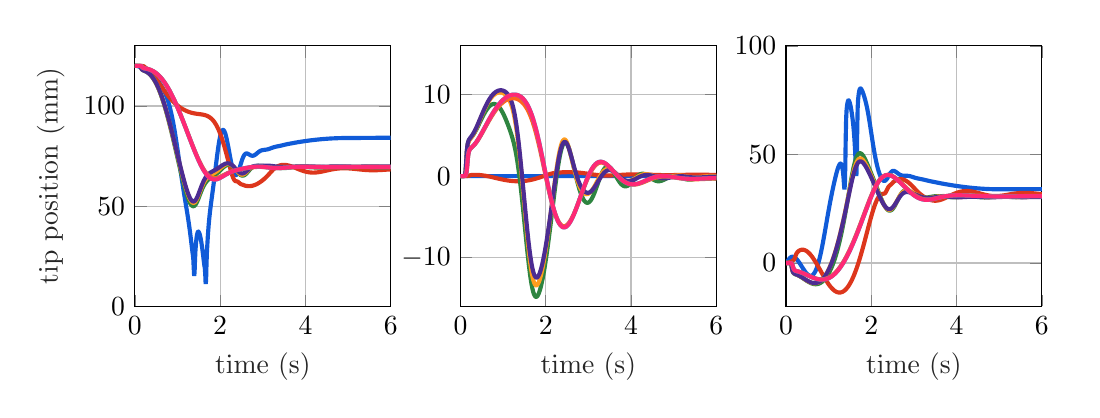
\begin{tikzpicture}

\begin{axis}[%
width=0.268\textwidth,
height=0.273\textwidth,
at={(0\textwidth,0\textwidth)},
scale only axis,
xmin=0,
xmax=6,
xlabel style={font=\color{white!15!black}},
xlabel={time (s)},
ymin=0,
ymax=130,
ylabel style={font=\color{white!15!black}},
ylabel={tip position (mm)},
axis background/.style={fill=white},
xmajorgrids,
ymajorgrids
]
\addplot [color=mycolor1, line width=1.5pt, forget plot]
  table[row sep=crcr]{%
0	119.999999824351\\
0.01	119.999761006601\\
0.02	119.996496846166\\
0.03	119.985718557839\\
0.04	119.964880088242\\
0.05	119.932615064138\\
0.06	119.889113056561\\
0.07	119.834971168929\\
0.08	119.771232053867\\
0.09	119.698883594988\\
0.1	119.618976052914\\
0.11	119.532387253545\\
0.12	119.439967448317\\
0.13	119.342396849961\\
0.14	119.240315312118\\
0.15	119.134221106263\\
0.16	119.024574745018\\
0.17	118.911723223345\\
0.18	118.795980138295\\
0.19	118.677568653634\\
0.2	118.556682579098\\
0.21	118.433443910826\\
0.22	118.307949170363\\
0.23	118.180238402931\\
0.24	118.050329515685\\
0.25	117.918196859364\\
0.26	117.783796300099\\
0.27	117.647050825152\\
0.28	117.507868093802\\
0.29	117.366132448605\\
0.3	117.221715873008\\
0.31	117.074474968299\\
0.32	116.924256085862\\
0.33	116.770896825164\\
0.34	116.614226581768\\
0.35	116.454071371469\\
0.36	116.290250163843\\
0.37	116.122582663887\\
0.38	115.950881994903\\
0.39	115.774964855416\\
0.4	115.594641170433\\
0.41	115.409725989712\\
0.42	115.220026140091\\
0.43	115.025353830792\\
0.44	114.825511278079\\
0.45	114.6203050157\\
0.46	114.409528667674\\
0.47	114.19297781361\\
0.48	113.970431366578\\
0.49	113.741666546228\\
0.5	113.506439320119\\
0.51	113.26449907836\\
0.52	113.01556848251\\
0.53	112.759357593083\\
0.54	112.495544085454\\
0.55	112.223785933177\\
0.56	111.943701974316\\
0.57	111.654883285866\\
0.58	111.356875160517\\
0.59	111.049186862381\\
0.6	110.731275262822\\
0.61	110.402552370005\\
0.62	110.062371175112\\
0.63	109.710030576761\\
0.64	109.344765679087\\
0.65	108.965750132387\\
0.66	108.572090469545\\
0.67	108.162824947057\\
0.68	107.736923681697\\
0.69	107.293284732\\
0.7	106.830740839743\\
0.71	106.348051858033\\
0.72	105.843919949\\
0.73	105.316978759632\\
0.74	104.765818020413\\
0.75	104.188969915192\\
0.76	103.584941931931\\
0.77	102.952203871275\\
0.78	102.289227928714\\
0.79	101.594479565251\\
0.8	100.866461926607\\
0.81	100.103710511407\\
0.82	99.3048447934397\\
0.83	98.4685642921724\\
0.84	97.5937084703769\\
0.85	96.6792513284613\\
0.86	95.7243693186971\\
0.87	94.7284338747264\\
0.88	93.6910840884815\\
0.89	92.6122140234625\\
0.9	91.4920477315701\\
0.91	90.331117496065\\
0.92	89.1303344501962\\
0.93	87.890955466455\\
0.94	86.6146466057379\\
0.95	85.3034288947525\\
0.96	83.9597403267121\\
0.97	82.5863444921697\\
0.98	81.1863913044906\\
0.99	79.7632824471517\\
1	78.3207349808177\\
1.01	76.862609158136\\
1.02	75.3929583165023\\
1.03	73.9158381233124\\
1.04	72.4353430744522\\
1.05	70.9554053657524\\
1.06	69.479821213836\\
1.07	68.0120522176315\\
1.08	66.5552500069188\\
1.09	65.112070980448\\
1.1	63.684707653561\\
1.11	62.2747260899165\\
1.12	60.8831103150038\\
1.13	59.5101283065856\\
1.14	58.1553925796929\\
1.15	56.8177565082787\\
1.16	55.4953906316062\\
1.17	54.1857073647971\\
1.18	52.885453351008\\
1.19	51.5906446741126\\
1.2	50.2966841931333\\
1.21	48.9983021544355\\
1.22	47.6896828069595\\
1.23	46.3644249125003\\
1.24	45.0156729663339\\
1.25	43.6361229825178\\
1.26	42.2181976301616\\
1.27	40.7541788096905\\
1.28	39.2365684654916\\
1.29	37.6586131046146\\
1.3	36.0153135263962\\
1.31	34.3052099274029\\
1.32	32.5336771995047\\
1.33	30.7191749438592\\
1.34	28.9054585390978\\
1.35	27.1868248823313\\
1.36	25.7641139588364\\
1.37	23.7389391233212\\
1.38	19.3350211852975\\
1.39	15.2538925166398\\
1.4	16.8089911140614\\
1.41	22.9813966198814\\
1.42	27.5893513818984\\
1.43	30.5631865870065\\
1.44	32.9554354592321\\
1.45	34.729879863386\\
1.46	35.9827973597344\\
1.47	36.770680025833\\
1.48	37.1772604175127\\
1.49	37.2542470310477\\
1.5	37.0599251420584\\
1.51	36.630939585206\\
1.52	36.0029125464571\\
1.53	35.1977061797354\\
1.54	34.2343819593173\\
1.55	33.1239310653069\\
1.56	31.8750304145053\\
1.57	30.4928159755338\\
1.58	28.9825110101808\\
1.59	27.3518917808935\\
1.6	25.6166950482456\\
1.61	23.8114558414142\\
1.62	22.0088089384839\\
1.63	20.3648618177955\\
1.64	19.2100048676026\\
1.65	16.2953511213352\\
1.66	11.2311103659594\\
1.67	13.0020331372442\\
1.68	21.322763212686\\
1.69	27.1282990723681\\
1.7	30.9973275550963\\
1.71	34.5741203246097\\
1.72	37.6709417498994\\
1.73	40.4085436565868\\
1.74	42.8025839962144\\
1.75	44.9553130469619\\
1.76	46.8967165638708\\
1.77	48.7010375052856\\
1.78	50.3948803576434\\
1.79	52.0286779966581\\
1.8	53.6206764859965\\
1.81	55.2032157379555\\
1.82	56.7861825055777\\
1.83	58.3885132293256\\
1.84	60.01279231464\\
1.85	61.6677659289419\\
1.86	63.3497434162017\\
1.87	65.059457884914\\
1.88	66.7879260403827\\
1.89	68.52963370126\\
1.9	70.2714955019447\\
1.91	72.0035460958136\\
1.92	73.7101393463483\\
1.93	75.3788277127393\\
1.94	76.9932010338721\\
1.95	78.5403341913678\\
1.96	80.0048223405911\\
1.97	81.3750163773188\\
1.98	82.6379178556449\\
1.99	83.7843841218846\\
2	84.8046513587129\\
2.01	85.6926903789515\\
2.02	86.4422318112658\\
2.03	87.0504431235982\\
2.04	87.514398435123\\
2.05	87.8342344105785\\
2.06	88.010030815908\\
2.07	88.0445498681167\\
2.08	87.9405145674255\\
2.09	87.7029801146142\\
2.1	87.3370029755592\\
2.11	86.8496563636592\\
2.12	86.2480473850792\\
2.13	85.5410019237123\\
2.14	84.7374355161328\\
2.15	83.847682250718\\
2.16	82.8821600529965\\
2.17	81.8523599528936\\
2.18	80.7698333087609\\
2.19	79.646904686426\\
2.2	78.4958652247314\\
2.21	77.3293881974067\\
2.22	76.1599852695569\\
2.23	75.0001922077615\\
2.24	73.8622163138894\\
2.25	72.7579819319192\\
2.26	71.6989145427131\\
2.27	70.6958684891569\\
2.28	69.7590266697855\\
2.29	68.8978022754576\\
2.3	68.1207645351111\\
2.31	67.4355463315514\\
2.32	66.8487516684116\\
2.33	66.3658806209972\\
2.34	65.9911905871545\\
2.35	65.7276394934708\\
2.36	65.5766766680308\\
2.37	65.5382340919874\\
2.38	65.6104568662753\\
2.39	65.7898243382961\\
2.4	66.0708340126949\\
2.41	66.4463093094803\\
2.42	66.9071469050241\\
2.43	67.4428044040451\\
2.44	68.041103714966\\
2.45	68.6889658892634\\
2.46	69.3723203912822\\
2.47	70.0769857479727\\
2.48	70.7885953630211\\
2.49	71.4935066475941\\
2.5	72.178697566217\\
2.51	72.8326017323247\\
2.52	73.4449118604577\\
2.53	74.0072539133297\\
2.54	74.5128800239664\\
2.55	74.9571340996971\\
2.56	75.3370592079007\\
2.57	75.6516818198894\\
2.58	75.9015521474145\\
2.59	76.0889040446052\\
2.6	76.2171638582587\\
2.61	76.2910014498474\\
2.62	76.3158828947013\\
2.63	76.2980955983085\\
2.64	76.2443219358967\\
2.65	76.161610851013\\
2.66	76.0570507527853\\
2.67	75.9377442659272\\
2.68	75.8105110751725\\
2.69	75.6818432203793\\
2.7	75.5576966456964\\
2.71	75.4435286962728\\
2.72	75.3440824875432\\
2.73	75.2634024485909\\
2.74	75.2047054979731\\
2.75	75.1704270753034\\
2.76	75.1621091742696\\
2.77	75.1805218574326\\
2.78	75.2255933797672\\
2.79	75.296481348591\\
2.8	75.3915909178757\\
2.81	75.5087553539008\\
2.82	75.6452200800347\\
2.83	75.7978721380976\\
2.84	75.963243032824\\
2.85	76.1377325178123\\
2.86	76.3176319933859\\
2.87	76.4993362283317\\
2.88	76.6793633067224\\
2.89	76.8545832719665\\
2.9	77.0221784597252\\
2.91	77.1798205144795\\
2.92	77.3256112010433\\
2.93	77.4582205297882\\
2.94	77.5768020788827\\
2.95	77.6810738961919\\
2.96	77.7711760150732\\
2.97	77.8477383285003\\
2.98	77.9117440308151\\
2.99	77.9645448093854\\
3	78.0077140455007\\
3.01	78.0430457060451\\
3.02	78.0724108082485\\
3.03	78.0977608873374\\
3.04	78.1209851748228\\
3.05	78.1438857391827\\
3.06	78.1680839907899\\
3.07	78.1950324612075\\
3.08	78.2259214073157\\
3.09	78.261704189547\\
3.1	78.3030314087901\\
3.11	78.3502959083633\\
3.12	78.4035892453636\\
3.13	78.4627668441313\\
3.14	78.5274227629503\\
3.15	78.5969574891257\\
3.16	78.6705779879866\\
3.17	78.7474134178356\\
3.18	78.826489546461\\
3.19	78.9068187850759\\
3.2	78.9873965991384\\
3.21	79.067291582938\\
3.22	79.145630366044\\
3.23	79.2216776561125\\
3.24	79.2948094848828\\
3.25	79.3645779625387\\
3.26	79.4306715868051\\
3.27	79.4929630875179\\
3.28	79.5514578643693\\
3.29	79.6063261406188\\
3.3	79.6578426487787\\
3.31	79.7064065547255\\
3.32	79.7524913845311\\
3.33	79.7966433060696\\
3.34	79.839393507196\\
3.35	79.8812894009318\\
3.36	79.9228417282843\\
3.37	79.9645324425972\\
3.38	80.0067649397883\\
3.39	80.0498824625666\\
3.4	80.0941268280084\\
3.41	80.1396650501282\\
3.42	80.1865576914593\\
3.43	80.2347935810503\\
3.44	80.2842665633455\\
3.45	80.3348168175165\\
3.46	80.3862135723966\\
3.47	80.4382003714997\\
3.48	80.4904806826947\\
3.49	80.5427638654243\\
3.5	80.5947505666758\\
3.51	80.646176215397\\
3.52	80.6967936283802\\
3.53	80.7464115227664\\
3.54	80.7948727161189\\
3.55	80.842086229659\\
3.56	80.8880006308934\\
3.57	80.9326295444866\\
3.58	80.9760208047223\\
3.59	81.0182763351319\\
3.6	81.05951863982\\
3.61	81.0999068384572\\
3.62	81.1396024860927\\
3.63	81.1787839381913\\
3.64	81.2176146873966\\
3.65	81.256254409671\\
3.66	81.2948351078373\\
3.67	81.3334698466427\\
3.68	81.372236066548\\
3.69	81.4111862156713\\
3.7	81.4503351396888\\
3.71	81.4896738365588\\
3.72	81.5291603342429\\
3.73	81.568735915289\\
3.74	81.6083183974979\\
3.75	81.6478196365807\\
3.76	81.6871398548199\\
3.77	81.7261850250984\\
3.78	81.7648609202483\\
3.79	81.8030890975276\\
3.8	81.8407996395257\\
3.81	81.8779451155642\\
3.82	81.9144907400809\\
3.83	81.9504265328052\\
3.84	81.9857543247636\\
3.85	82.0204986595586\\
3.86	82.0546921178108\\
3.87	82.0883842635341\\
3.88	82.1216263241668\\
3.89	82.1544791633113\\
3.9	82.1869981754254\\
3.91	82.2192412155069\\
3.92	82.2512544832593\\
3.93	82.2830811688312\\
3.94	82.3147488399477\\
3.95	82.3462792492158\\
3.96	82.3776773964318\\
3.97	82.4089425705775\\
3.98	82.4400589137975\\
3.99	82.4710074321803\\
4	82.5017576215125\\
4.01	82.5322799443577\\
4.02	82.5625379378999\\
4.03	82.5925005664572\\
4.04	82.6221342428461\\
4.05	82.651414525667\\
4.06	82.6803176202852\\
4.07	82.7088310697789\\
4.08	82.736944520015\\
4.09	82.7646592945555\\
4.1	82.7919784483496\\
4.11	82.8189153554284\\
4.12	82.8454832786317\\
4.13	82.8717241647932\\
4.14	82.8976778195749\\
4.15	82.9233557035116\\
4.16	82.948759901181\\
4.17	82.973900456914\\
4.18	82.9987791008816\\
4.19	83.0234000692363\\
4.2	83.0477605029629\\
4.21	83.0718598737741\\
4.22	83.0956913174115\\
4.23	83.1192509252202\\
4.24	83.1425294922472\\
4.25	83.1655216900392\\
4.26	83.1882180033994\\
4.27	83.2106136997601\\
4.28	83.232700786448\\
4.29	83.2544766945414\\
4.3	83.2759361539451\\
4.31	83.2970795537151\\
4.32	83.3179046976417\\
4.33	83.3384148609485\\
4.34	83.3586104525497\\
4.35	83.3784968342176\\
4.36	83.3980759593142\\
4.37	83.4173540529751\\
4.38	83.4363333116627\\
4.39	83.4550195449093\\
4.4	83.4734140131942\\
4.41	83.4915211113308\\
4.42	83.5093403912024\\
4.43	83.5268743303961\\
4.44	83.5441205477069\\
4.45	83.5610796577673\\
4.46	83.5777476489808\\
4.47	83.5941237920763\\
4.48	83.6102031241009\\
4.49	83.625984355918\\
4.5	83.6414623978441\\
4.51	83.6566362091654\\
4.52	83.6715013064621\\
4.53	83.6860575137569\\
4.54	83.7003014169483\\
4.55	83.7142339956048\\
4.56	83.7278530129497\\
4.57	83.7411605378249\\
4.58	83.7541552849809\\
4.59	83.766840058122\\
4.6	83.7792367767739\\
4.61	83.7913718412716\\
4.62	83.8032313300837\\
4.63	83.81479999738\\
4.64	83.8260647404473\\
4.65	83.8370153472394\\
4.66	83.8476398929946\\
4.67	83.8579318442698\\
4.68	83.8678834695624\\
4.69	83.8774931483073\\
4.7	83.8867581211507\\
4.71	83.8956815977717\\
4.72	83.9042650625394\\
4.73	83.9125152033218\\
4.74	83.9204359635296\\
4.75	83.9280354174981\\
4.76	83.9353177638927\\
4.77	83.9422902995029\\
4.78	83.9489555145284\\
4.79	83.9553182859186\\
4.8	83.9613781711632\\
4.81	83.9671368774433\\
4.82	83.9726139586504\\
4.83	83.9778323120415\\
4.84	83.9827721224253\\
4.85	83.9874104460724\\
4.86	83.9917264544875\\
4.87	83.9957029516345\\
4.88	83.999321921322\\
4.89	84.0025721476883\\
4.9	84.0054426658468\\
4.91	84.0079303461824\\
4.92	84.0100324033526\\
4.93	84.0117760838079\\
4.94	84.0131891100722\\
4.95	84.014267330396\\
4.96	84.0149963067401\\
4.97	84.015372545264\\
4.98	84.0153893539516\\
4.99	84.0150463620537\\
5	84.0143407403291\\
5.01	84.01328107037\\
5.02	84.0118849275556\\
5.03	84.0102062601699\\
5.04	84.0083590729177\\
5.05	84.0065091491664\\
5.06	84.0048272454695\\
5.07	84.0034850323588\\
5.08	84.0026359794321\\
5.09	84.0024089216415\\
5.1	84.0028911557214\\
5.11	84.004129911007\\
5.12	84.0061225194491\\
5.13	84.0088155198691\\
5.14	84.012112892147\\
5.15	84.0159102013202\\
5.16	84.0200807259451\\
5.17	84.0244838460464\\
5.18	84.0289693361664\\
5.19	84.0333816765265\\
5.2	84.0375709328946\\
5.21	84.041430504011\\
5.22	84.0448848901174\\
5.23	84.0479025052965\\
5.24	84.050483025023\\
5.25	84.0526449779125\\
5.26	84.0544255728667\\
5.27	84.0558895556475\\
5.28	84.0571147199799\\
5.29	84.0581927099006\\
5.3	84.0592148494099\\
5.31	84.060272217953\\
5.32	84.0614528011899\\
5.33	84.062825730434\\
5.34	84.0644192724852\\
5.35	84.0662526223484\\
5.36	84.0683264314441\\
5.37	84.0706221886685\\
5.38	84.073100383118\\
5.39	84.0757096804144\\
5.4	84.0783853447934\\
5.41	84.0810603441119\\
5.42	84.0836642676973\\
5.43	84.0861344357763\\
5.44	84.088414027859\\
5.45	84.0904617862464\\
5.46	84.0922483130711\\
5.47	84.0937634994039\\
5.48	84.0950105383213\\
5.49	84.0960109023854\\
5.5	84.0967962912425\\
5.51	84.0974116477469\\
5.52	84.097905812708\\
5.53	84.0983335346449\\
5.54	84.098745899923\\
5.55	84.0991924506404\\
5.56	84.0997124379979\\
5.57	84.1003380081611\\
5.58	84.101087028421\\
5.59	84.1019678979693\\
5.6	84.102974224212\\
5.61	84.1040913046531\\
5.62	84.1052931056538\\
5.63	84.1065479150818\\
5.64	84.1078189605705\\
5.65	84.1090678981426\\
5.66	84.1102577620415\\
5.67	84.1113554586235\\
5.68	84.1123341216931\\
5.69	84.1131753006148\\
5.7	84.1138680794803\\
5.71	84.1144125916486\\
5.72	84.1148151542187\\
5.73	84.1150926083153\\
5.74	84.1152657186952\\
5.75	84.1153625156717\\
5.76	84.1154111438166\\
5.77	84.1154427867141\\
5.78	84.1154845680096\\
5.79	84.1155626766276\\
5.8	84.1156958732753\\
5.81	84.115899302301\\
5.82	84.1161789602918\\
5.83	84.1165364283474\\
5.84	84.1169643857293\\
5.85	84.1174522089952\\
5.86	84.1179823419473\\
5.87	84.1185364603172\\
5.88	84.1190923143004\\
5.89	84.1196300163251\\
5.9	84.1201288979458\\
5.91	84.1205734689917\\
5.92	84.1209498886042\\
5.93	84.1212512596144\\
5.94	84.1214734699173\\
5.95	84.1216196799019\\
5.96	84.1216955010557\\
5.97	84.121712750905\\
5.98	84.121684132794\\
5.99	84.121626506635\\
6	84.1215553681989\\
};
\addplot [color=mycolor2, line width=1.5pt, forget plot]
  table[row sep=crcr]{%
0	119.999999824351\\
0.01	119.999991014243\\
0.02	119.999889390258\\
0.03	119.999535485152\\
0.04	119.998760133155\\
0.05	119.997450471406\\
0.06	119.99556425031\\
0.07	119.993096079894\\
0.08	119.990055528429\\
0.09	119.98644623745\\
0.1	119.982253658257\\
0.11	119.977431382967\\
0.12	119.971887316802\\
0.13	119.965461526466\\
0.14	119.957891956261\\
0.15	119.94875563848\\
0.16	119.937365880138\\
0.17	119.922586963459\\
0.18	119.902484155936\\
0.19	119.873638120626\\
0.2	119.829731469497\\
0.21	119.758547913388\\
0.22	119.632125824298\\
0.23	119.452120620277\\
0.24	119.270573392396\\
0.25	119.095892886942\\
0.26	118.920562687553\\
0.27	118.746461169925\\
0.28	118.570543557777\\
0.29	118.392160759183\\
0.3	118.209679864761\\
0.31	118.022587980869\\
0.32	117.829999347684\\
0.33	117.631735749018\\
0.34	117.427358145997\\
0.35	117.216896616682\\
0.36	117.000169437522\\
0.37	116.777321745889\\
0.38	116.548325206553\\
0.39	116.313387081317\\
0.4	116.072574452595\\
0.41	115.826130169693\\
0.42	115.574184376322\\
0.43	115.317002432537\\
0.44	115.054758839496\\
0.45	114.78773466506\\
0.46	114.516137199768\\
0.47	114.240259137618\\
0.48	113.960332719654\\
0.49	113.676659267367\\
0.5	113.389490110614\\
0.51	113.09913257395\\
0.52	112.80585229305\\
0.53	112.509960064564\\
0.54	112.211731663557\\
0.55	111.911478828516\\
0.56	111.60948501054\\
0.57	111.306058592954\\
0.58	111.001486811379\\
0.59	110.696072852177\\
0.6	110.390103762794\\
0.61	110.083874418412\\
0.62	109.777667105762\\
0.63	109.471770397994\\
0.64	109.1664621135\\
0.65	108.862018245917\\
0.66	108.558706578545\\
0.67	108.256789167357\\
0.68	107.956521512043\\
0.69	107.658149628815\\
0.7	107.361914359162\\
0.71	107.068043760437\\
0.72	106.776761809795\\
0.73	106.488276867413\\
0.74	106.202794074612\\
0.75	105.920500581063\\
0.76	105.641581000041\\
0.77	105.366200027394\\
0.78	105.094520377379\\
0.79	104.826683362733\\
0.8	104.562828790004\\
0.81	104.303074015903\\
0.82	104.04753533168\\
0.83	103.796305960134\\
0.84	103.549478504668\\
0.85	103.307122303239\\
0.86	103.069306559473\\
0.87	102.83607482727\\
0.88	102.607477186905\\
0.89	102.383533494471\\
0.9	102.164273905076\\
0.91	101.949692050917\\
0.92	101.739804492664\\
0.93	101.534588518467\\
0.94	101.33404143738\\
0.95	101.138123976582\\
0.96	100.946817692875\\
0.97	100.760070146318\\
0.98	100.577849798897\\
0.99	100.400094048429\\
1	100.226761139714\\
1.01	100.057781326615\\
1.02	99.89310553836\\
1.03	99.7326598417732\\
1.04	99.5763906584371\\
1.05	99.4242226538981\\
1.06	99.2761003388218\\
1.07	99.1319467080821\\
1.08	98.9917104416173\\
1.09	98.8553161418647\\
1.1	98.7227187184908\\
1.11	98.5938442765424\\
1.12	98.4686519894912\\
1.13	98.3470684151032\\
1.14	98.2290529506526\\
1.15	98.114547657328\\
1.16	98.0035216352424\\
1.17	97.8959219141119\\
1.18	97.7917191519593\\
1.19	97.6908668011858\\
1.2	97.5933372210961\\
1.21	97.4990873678469\\
1.22	97.4080925337894\\
1.23	97.3203127306488\\
1.24	97.2357236424887\\
1.25	97.1542862191628\\
1.26	97.0759717538918\\
1.27	97.000741358597\\
1.28	96.9285586274876\\
1.29	96.8593836065715\\
1.3	96.79316942329\\
1.31	96.7298654566163\\
1.32	96.6694063077948\\
1.33	96.6117499939083\\
1.34	96.556821004292\\
1.35	96.5045670346454\\
1.36	96.4548883790715\\
1.37	96.4077223947361\\
1.38	96.3629453595199\\
1.39	96.3204761292755\\
1.4	96.2801732360473\\
1.41	96.2419357925005\\
1.42	96.2055997456435\\
1.43	96.171044680851\\
1.44	96.1380791400128\\
1.45	96.1065620775658\\
1.46	96.0762730875188\\
1.47	96.0470491626083\\
1.48	96.018639790224\\
1.49	95.9908589167903\\
1.5	95.9634269013751\\
1.51	95.9361347685793\\
1.52	95.9086669617821\\
1.53	95.880787158924\\
1.54	95.8521491634785\\
1.55	95.8224859745339\\
1.56	95.791435702678\\
1.57	95.758691862113\\
1.58	95.7238710124843\\
1.59	95.6866348336439\\
1.6	95.6465712163688\\
1.61	95.603315551249\\
1.62	95.5564269391217\\
1.63	95.5055154878688\\
1.64	95.4501124995528\\
1.65	95.3898039977496\\
1.66	95.3240949364316\\
1.67	95.252548839512\\
1.68	95.1746462117448\\
1.69	95.0899300965844\\
1.7	94.9978589278362\\
1.71	94.8979544740531\\
1.72	94.7896532283889\\
1.73	94.6724676070452\\
1.74	94.5458230966126\\
1.75	94.4092192662874\\
1.76	94.2620689680611\\
1.77	94.1038644593425\\
1.78	93.9340114443585\\
1.79	93.7519998403197\\
1.8	93.5572339386607\\
1.81	93.3492071984468\\
1.82	93.1273290703737\\
1.83	92.8911033364538\\
1.84	92.6399521324794\\
1.85	92.3733973342591\\
1.86	92.0908823490876\\
1.87	91.7919560130574\\
1.88	91.4760927635306\\
1.89	91.1428784693131\\
1.9	90.7918296398155\\
1.91	90.4225805619408\\
1.92	90.0347022456864\\
1.93	89.6278901894456\\
1.94	89.2017838052031\\
1.95	88.7561540788304\\
1.96	88.2907242596794\\
1.97	87.8053566237652\\
1.98	87.2998752464595\\
1.99	86.7742510077556\\
2	86.2284326485994\\
2.01	85.6625105143896\\
2.02	85.0765762102495\\
2.03	84.4708587959191\\
2.04	83.8456180826774\\
2.05	83.2012478366063\\
2.06	82.5381923012224\\
2.07	81.8570342746568\\
2.08	81.1584203493573\\
2.09	80.4431441521623\\
2.1	79.712076420178\\
2.11	78.9662429644319\\
2.12	78.206756541475\\
2.13	77.434892069354\\
2.14	76.6520244738696\\
2.15	75.8596972807198\\
2.16	75.0595654043277\\
2.17	74.2534592966739\\
2.18	73.4433345618087\\
2.19	72.631333443249\\
2.2	71.8197454864447\\
2.21	71.0110724596337\\
2.22	70.2080106162675\\
2.23	69.4135357591039\\
2.24	68.6309345517931\\
2.25	67.8639538770113\\
2.26	67.1169505627966\\
2.27	66.3952078645816\\
2.28	65.7053319047871\\
2.29	65.0558229059067\\
2.3	64.4575351704136\\
2.31	63.9235870704571\\
2.32	63.4677603835671\\
2.33	63.1012375151511\\
2.34	62.8284861616922\\
2.35	62.644547983156\\
2.36	62.534616359027\\
2.37	62.4760512955619\\
2.38	62.4420103035562\\
2.39	62.4062851268204\\
2.4	62.3479285153312\\
2.41	62.254604652177\\
2.42	62.1234829898326\\
2.43	61.9601941609231\\
2.44	61.7762579741385\\
2.45	61.5861560820988\\
2.46	61.4041584674015\\
2.47	61.2416516064435\\
2.48	61.1050462374021\\
2.49	60.9950317324375\\
2.5	60.9070807035666\\
2.51	60.8333627998149\\
2.52	60.7651282272565\\
2.53	60.6951960243614\\
2.54	60.6195625400608\\
2.55	60.5380574382983\\
2.56	60.4536422153857\\
2.57	60.3711010781691\\
2.58	60.2953804072076\\
2.59	60.2302872243378\\
2.6	60.1775443261811\\
2.61	60.1367360517263\\
2.62	60.1057569128657\\
2.63	60.0818222252687\\
2.64	60.0624191466328\\
2.65	60.0460724293189\\
2.66	60.0324979972274\\
2.67	60.0225616257068\\
2.68	60.0177635837788\\
2.69	60.0196731677838\\
2.7	60.029421261722\\
2.71	60.0474079938301\\
2.72	60.0733538541455\\
2.73	60.1064633423939\\
2.74	60.1458303949559\\
2.75	60.1906590219005\\
2.76	60.240544861674\\
2.77	60.2954235157749\\
2.78	60.3555702957541\\
2.79	60.4213449396089\\
2.8	60.4931290012296\\
2.81	60.5710993990504\\
2.82	60.655234163101\\
2.83	60.7452810780974\\
2.84	60.840946082873\\
2.85	60.9418737544041\\
2.86	61.047819153412\\
2.87	61.1585800253725\\
2.88	61.2740940284376\\
2.89	61.3943205644766\\
2.9	61.5192891128679\\
2.91	61.6489887754099\\
2.92	61.7834229280178\\
2.93	61.9225296771411\\
2.94	62.0662621037112\\
2.95	62.214523630515\\
2.96	62.3672606616835\\
2.97	62.5243942864785\\
2.98	62.6859179988244\\
2.99	62.8518079968958\\
3	63.0220924601612\\
3.01	63.1967772438258\\
3.02	63.3759333394589\\
3.03	63.5595959115154\\
3.04	63.7478503595305\\
3.05	63.9407416835083\\
3.06	64.1383455780229\\
3.07	64.3406662953179\\
3.08	64.5477151740312\\
3.09	64.7594089574876\\
3.1	64.9756433532311\\
3.11	65.1961912312517\\
3.12	65.4207692657188\\
3.13	65.6489444539489\\
3.14	65.8802174667792\\
3.15	66.1139288857918\\
3.16	66.3493381972315\\
3.17	66.5855535975393\\
3.18	66.8216241191684\\
3.19	67.0564849316166\\
3.2	67.2890583334487\\
3.21	67.5182119408859\\
3.22	67.7428616710948\\
3.23	67.9619351067715\\
3.24	68.174471688515\\
3.25	68.3795662119303\\
3.26	68.5764841734333\\
3.27	68.7645688231607\\
3.28	68.9433584365053\\
3.29	69.1124844111951\\
3.3	69.271761648516\\
3.31	69.4210576480743\\
3.32	69.5603945478087\\
3.33	69.6898424705855\\
3.34	69.8095876156189\\
3.35	69.9198298185797\\
3.36	70.0208503520139\\
3.37	70.1129027338157\\
3.38	70.1963131914935\\
3.39	70.2713489320793\\
3.4	70.3383139765104\\
3.41	70.3974478430752\\
3.42	70.4490311133011\\
3.43	70.49327127563\\
3.44	70.5304216708848\\
3.45	70.5606644605543\\
3.46	70.5842246981071\\
3.47	70.6012731047343\\
3.48	70.6120186097272\\
3.49	70.6166310738585\\
3.5	70.6153059166831\\
3.51	70.6082318461\\
3.52	70.5955843519204\\
3.53	70.5775738816009\\
3.54	70.5543710709503\\
3.55	70.5261958680561\\
3.56	70.4932253606245\\
3.57	70.4556887579617\\
3.58	70.4137634327165\\
3.59	70.3676881637239\\
3.6	70.3176391509763\\
3.61	70.2638494658541\\
3.62	70.2064990569033\\
3.63	70.1458156823993\\
3.64	70.0819781386178\\
3.65	70.015213216771\\
3.66	69.9456939665844\\
3.67	69.8736463600372\\
3.68	69.7992380869771\\
3.69	69.7226944426901\\
3.7	69.6441786182201\\
3.71	69.5639154699675\\
3.72	69.4820645086297\\
3.73	69.398850178377\\
3.74	69.3144288088151\\
3.75	69.2290240649318\\
3.76	69.1427891590811\\
3.77	69.0559461789348\\
3.78	68.9686448633715\\
3.79	68.8811045622248\\
3.8	68.7934708613947\\
3.81	68.7059589720602\\
3.82	68.618709450233\\
3.83	68.53193185578\\
3.84	68.4457607559516\\
3.85	68.3603985394437\\
3.86	68.2759728281281\\
3.87	68.1926773816941\\
3.88	68.1106319715586\\
3.89	68.0300203692083\\
3.9	67.9509536638917\\
3.91	67.8736043928131\\
3.92	67.7980742108643\\
3.93	67.7245232921399\\
3.94	67.6530431856881\\
3.95	67.5837806935636\\
3.96	67.5168166709604\\
3.97	67.4522836642544\\
3.98	67.3902513366055\\
3.99	67.3308372286013\\
4	67.2740994115522\\
4.01	67.2201398124142\\
4.02	67.1690046170367\\
4.03	67.1207796795395\\
4.04	67.0754943536191\\
4.05	67.0332244477558\\
4.06	66.9939844632743\\
4.07	66.9578368444671\\
4.08	66.9247842164805\\
4.09	66.8948750037629\\
4.1	66.8680954579823\\
4.11	66.8444782164148\\
4.12	66.8239959358318\\
4.13	66.8066631420567\\
4.14	66.7924395825526\\
4.15	66.7813269656948\\
4.16	66.7732751519146\\
4.17	66.7682702971006\\
4.18	66.7662526118617\\
4.19	66.7671930654816\\
4.2	66.7710262074505\\
4.21	66.7777053390075\\
4.22	66.7871621455529\\
4.23	66.7993276026337\\
4.24	66.8141328761375\\
4.25	66.8314864384703\\
4.26	66.8513167169534\\
4.27	66.8735184135005\\
4.28	66.8980179307098\\
4.29	66.9247006811034\\
4.3	66.9534892067528\\
4.31	66.9842584563743\\
4.32	67.0169238857711\\
4.33	67.0513577557331\\
4.34	67.0874716475665\\
4.35	67.1251349171016\\
4.36	67.1642585819828\\
4.37	67.2047069536165\\
4.38	67.2463917854289\\
4.39	67.2891737380433\\
4.4	67.332966313641\\
4.41	67.3776281155878\\
4.42	67.4230754289754\\
4.43	67.4691664134892\\
4.44	67.5158211239346\\
4.45	67.5628988177836\\
4.46	67.6103241882748\\
4.47	67.6579589958128\\
4.48	67.7057332798023\\
4.49	67.7535125395551\\
4.5	67.8012326939997\\
4.51	67.8487640421109\\
4.52	67.8960487498293\\
4.53	67.9429628121473\\
4.54	67.9894548634674\\
4.55	68.0354073441366\\
4.56	68.0807754544798\\
4.57	68.1254486990626\\
4.58	68.1693888364101\\
4.59	68.2124929359508\\
4.6	68.2547292154073\\
4.61	68.2960026993505\\
4.62	68.3362878844632\\
4.63	68.3754980356665\\
4.64	68.4136136755128\\
4.65	68.4505564944312\\
4.66	68.4863127237052\\
4.67	68.5208125708485\\
4.68	68.5540476051236\\
4.69	68.5859565577494\\
4.7	68.6165359238556\\
4.71	68.6457328905821\\
4.72	68.6735484389259\\
4.73	68.6999380814134\\
4.74	68.7249068307391\\
4.75	68.7484138440626\\
4.76	68.7704737436526\\
4.77	68.7910512121444\\
4.78	68.8101668540018\\
4.79	68.8277933239703\\
4.8	68.8439564173182\\
4.81	68.8586318160294\\
4.82	68.8718481132328\\
4.83	68.8835822328308\\
4.84	68.893868224394\\
4.85	68.9026909313403\\
4.86	68.9100853896975\\
4.87	68.9160471688783\\
4.88	68.9206076742636\\
4.89	68.9237733614443\\
4.9	68.9255732930998\\
4.91	68.9260225476212\\
4.92	68.9251462098267\\
4.93	68.9229694899718\\
4.94	68.9195115923975\\
4.95	68.9148101072046\\
4.96	68.9088784406531\\
4.97	68.9017618860993\\
4.98	68.8934734391236\\
4.99	68.8840655413847\\
5	68.8735506862255\\
5.01	68.8619895040063\\
5.02	68.8493967945998\\
5.03	68.8358381663595\\
5.04	68.8213349655769\\
5.05	68.8059594766664\\
5.06	68.7897340099153\\
5.07	68.7727355477038\\
5.08	68.7549841963492\\
5.09	68.7365548344142\\
5.1	68.7174701482186\\
5.11	68.6978030025026\\
5.12	68.6775773082687\\
5.13	68.6568663080758\\
5.14	68.6356922048798\\
5.15	68.6141291831796\\
5.16	68.592198514371\\
5.17	68.56997563143\\
5.18	68.5474815943066\\
5.19	68.5247930966385\\
5.2	68.5019313517597\\
5.21	68.4789739408536\\
5.22	68.4559422159625\\
5.23	68.432913948247\\
5.24	68.4099103406396\\
5.25	68.3870084751798\\
5.26	68.36422899433\\
5.27	68.3416473793276\\
5.28	68.3192833053732\\
5.29	68.2972098154017\\
5.3	68.2754452899305\\
5.31	68.2540596193451\\
5.32	68.2330696611298\\
5.33	68.2125415627691\\
5.34	68.1924905108698\\
5.35	68.1729784169201\\
5.36	68.1540186950464\\
5.37	68.1356727029492\\
5.38	68.1179466812812\\
5.39	68.100899545902\\
5.4	68.0845324049883\\
5.41	68.0688987964556\\
5.42	68.0539985749585\\
5.43	68.0398793293464\\
5.44	68.026535335554\\
5.45	68.0140138535607\\
5.46	68.0023056104412\\
5.47	67.9914538159594\\
5.48	67.9814481258428\\
5.49	67.9723231529762\\
5.5	67.964067799236\\
5.51	67.956707734423\\
5.52	67.9502311909773\\
5.53	67.9446579565933\\
5.54	67.9399720919519\\
5.55	67.9361862576654\\
5.56	67.9332825323362\\
5.57	67.9312644727214\\
5.58	67.9301158221433\\
5.59	67.9298312550083\\
5.6	67.9303964064977\\
5.61	67.9317977984955\\
5.62	67.9340229197029\\
5.63	67.9370489341108\\
5.64	67.9408650875798\\
5.65	67.9454414716547\\
5.66	67.9507690670935\\
5.67	67.9568103447718\\
5.68	67.9635579155508\\
5.69	67.9709672716591\\
5.7	67.9790288330524\\
5.71	67.9876965694074\\
5.72	67.99695939955\\
5.73	68.0067696215038\\
5.74	68.0171167239211\\
5.75	68.0279489081379\\
5.76	68.0392564277618\\
5.77	68.0509839140819\\
5.78	68.0631224873556\\
5.79	68.0756138959335\\
5.8	68.0884502721642\\
5.81	68.1015712115576\\
5.82	68.1149700045929\\
5.83	68.1285848121902\\
5.84	68.1424101923967\\
5.85	68.1563835453491\\
5.86	68.1705007531021\\
5.87	68.184699072751\\
5.88	68.1989757155504\\
5.89	68.213268360455\\
5.9	68.2275755141747\\
5.91	68.2418357994304\\
5.92	68.2560489606391\\
5.93	68.2701550527625\\
5.94	68.2841549881963\\
5.95	68.2979907145693\\
5.96	68.3116642373292\\
5.97	68.3251198295373\\
5.98	68.3383605114872\\
5.99	68.3513332834609\\
6	68.3640420980248\\
};
\addplot [color=mycolor3, line width=1.5pt, forget plot]
  table[row sep=crcr]{%
0	119.999999824351\\
0.01	119.999999823849\\
0.02	119.99999982016\\
0.03	119.999999792279\\
0.04	119.999999603748\\
0.05	119.999998628326\\
0.06	119.999994296716\\
0.07	119.99997572178\\
0.08	119.999892691566\\
0.09	119.999492399102\\
0.1	119.997398205762\\
0.11	119.981815462772\\
0.12	119.89815396777\\
0.13	119.648152329234\\
0.14	119.225177632991\\
0.15	118.780571852625\\
0.16	118.435002635377\\
0.17	118.184066668593\\
0.18	117.999634077072\\
0.19	117.859559905154\\
0.2	117.746123993776\\
0.21	117.647663755165\\
0.22	117.555918621618\\
0.23	117.465598571318\\
0.24	117.372908038536\\
0.25	117.275423893\\
0.26	117.171273410429\\
0.27	117.059245989296\\
0.28	116.938291283199\\
0.29	116.80771173568\\
0.3	116.666820293407\\
0.31	116.515145019628\\
0.32	116.352172701358\\
0.33	116.17753992529\\
0.34	115.990828897499\\
0.35	115.791737382328\\
0.36	115.57990979986\\
0.37	115.355086009338\\
0.38	115.116958289631\\
0.39	114.865300944824\\
0.4	114.599847209012\\
0.41	114.320403354038\\
0.42	114.026740520941\\
0.43	113.718696303003\\
0.44	113.39607771947\\
0.45	113.058753088018\\
0.46	112.706564738964\\
0.47	112.339411529575\\
0.48	111.957171138423\\
0.49	111.559773228602\\
0.5	111.147130664132\\
0.51	110.719204273602\\
0.52	110.275942027403\\
0.53	109.817336252152\\
0.54	109.34336994505\\
0.55	108.85406716544\\
0.56	108.349445788037\\
0.57	107.829561691911\\
0.58	107.294467360348\\
0.59	106.744250399051\\
0.6	106.178997479915\\
0.61	105.598827646155\\
0.62	105.003861172941\\
0.63	104.394248055064\\
0.64	103.770141421022\\
0.65	103.131721547081\\
0.66	102.479173514389\\
0.67	101.812707050597\\
0.68	101.132537341932\\
0.69	100.438903571432\\
0.7	99.7320500363449\\
0.71	99.0122450055057\\
0.72	98.2797601785442\\
0.73	97.5348910657643\\
0.74	96.7779359300982\\
0.75	96.0092158675055\\
0.76	95.2290553119858\\
0.77	94.4377998961731\\
0.78	93.6357992412522\\
0.79	92.823422660152\\
0.8	92.0010441402847\\
0.81	91.1690560282983\\
0.82	90.3278560979687\\
0.83	89.4778593579645\\
0.84	88.619487099992\\
0.85	87.7531769700782\\
0.86	86.8793738944855\\
0.87	85.9985385556746\\
0.88	85.1111400943892\\
0.89	84.2176631340292\\
0.9	83.3186021566894\\
0.91	82.414467224059\\
0.92	81.5057799231747\\
0.93	80.5930779379353\\
0.94	79.6769124568998\\
0.95	78.7578517567091\\
0.96	77.8364799593206\\
0.97	76.9133997964811\\
0.98	75.9892325971152\\
0.99	75.0646204096738\\
1	74.1402270916359\\
1.01	73.216738568695\\
1.02	72.2948692146272\\
1.03	71.3753562379476\\
1.04	70.4589734625252\\
1.05	69.5465172958856\\
1.06	68.6388284453076\\
1.07	67.7367724694264\\
1.08	66.8412661495421\\
1.09	65.9532565644843\\
1.1	65.0737480651191\\
1.11	64.2037814766208\\
1.12	63.3444614587621\\
1.13	62.4969359677818\\
1.14	61.6624238708928\\
1.15	60.8421947703259\\
1.16	60.037596806297\\
1.17	59.2500369100186\\
1.18	58.4810087924473\\
1.19	57.7320735947909\\
1.2	57.0048863553233\\
1.21	56.3011804837791\\
1.22	55.6227967383464\\
1.23	54.9716577280868\\
1.24	54.3497962502536\\
1.25	53.7593335523021\\
1.26	53.202503044241\\
1.27	52.6816205057491\\
1.28	52.1991009190681\\
1.29	51.7574122121614\\
1.3	51.3590953580861\\
1.31	51.0066707995272\\
1.32	50.7026702380949\\
1.33	50.4494924977539\\
1.34	50.2494311076526\\
1.35	50.1044959986815\\
1.36	50.0164280746365\\
1.37	49.9864983422979\\
1.38	50.015523414641\\
1.39	50.1036596929006\\
1.4	50.2504431184724\\
1.41	50.4546034367809\\
1.42	50.7141499888445\\
1.43	51.0262483025054\\
1.44	51.3873431099856\\
1.45	51.7931242584356\\
1.46	52.2386969168658\\
1.47	52.7186146923828\\
1.48	53.2270983388553\\
1.49	53.7581021371229\\
1.5	54.3055547464764\\
1.51	54.8634295731772\\
1.52	55.4259721481638\\
1.53	55.9877479958055\\
1.54	56.5438268911362\\
1.55	57.0897911805644\\
1.56	57.6218598229947\\
1.57	58.1368528379402\\
1.58	58.6322544006542\\
1.59	59.106133038058\\
1.6	59.5571654885955\\
1.61	59.9845240951982\\
1.62	60.3878714468617\\
1.63	60.767244739106\\
1.64	61.1230282831834\\
1.65	61.4558616503098\\
1.66	61.7666106695821\\
1.67	62.0562837664917\\
1.68	62.3260166442761\\
1.69	62.5770209539934\\
1.7	62.8105741158074\\
1.71	63.0279900730129\\
1.72	63.2306157544909\\
1.73	63.4198256897045\\
1.74	63.5969989222251\\
1.75	63.7635375727856\\
1.76	63.9208420364081\\
1.77	64.0703322682206\\
1.78	64.2133945950707\\
1.79	64.3514404122418\\
1.8	64.485817907999\\
1.81	64.6178892921237\\
1.82	64.7489227789697\\
1.83	64.8801693797351\\
1.84	65.0127648471109\\
1.85	65.1477947009425\\
1.86	65.2862099532619\\
1.87	65.4288793380332\\
1.88	65.5765077278507\\
1.89	65.7297034680598\\
1.9	65.8888933943768\\
1.91	66.0543972882005\\
1.92	66.2263430277374\\
1.93	66.404749605581\\
1.94	66.5894421132691\\
1.95	66.7801430826983\\
1.96	66.976386948142\\
1.97	67.1776191048837\\
1.98	67.383109284631\\
1.99	67.5920575541778\\
2	67.8035059623882\\
2.01	68.0164506158829\\
2.02	68.2297509872217\\
2.03	68.4422471725674\\
2.04	68.6526663586147\\
2.05	68.8597430131321\\
2.06	69.0621237230357\\
2.07	69.258493868446\\
2.08	69.447475232989\\
2.09	69.6277535605851\\
2.1	69.7979758232369\\
2.11	69.9568793496998\\
2.12	70.1031855704684\\
2.13	70.2357303026678\\
2.14	70.3533549111215\\
2.15	70.4550368639698\\
2.16	70.5397808418356\\
2.17	70.6067470375154\\
2.18	70.6551367843998\\
2.19	70.6843238077379\\
2.2	70.6937430480758\\
2.21	70.6830165122351\\
2.22	70.6518429082477\\
2.23	70.6001206732221\\
2.24	70.5278397427455\\
2.25	70.4352001451695\\
2.26	70.3225071719353\\
2.27	70.190284088364\\
2.28	70.0391718257703\\
2.29	69.87003414713\\
2.3	69.6838628554242\\
2.31	69.4818734849864\\
2.32	69.26541682982\\
2.33	69.0360629361455\\
2.34	68.7955194962304\\
2.35	68.5457016202043\\
2.36	68.2886573375209\\
2.37	68.0266203778397\\
2.38	67.7619427278369\\
2.39	67.4971275335932\\
2.4	67.234768475608\\
2.41	66.9775600370786\\
2.42	66.7282483639856\\
2.43	66.4896069526451\\
2.44	66.2643863674144\\
2.45	66.055286998734\\
2.46	65.864922253468\\
2.47	65.6957423601187\\
2.48	65.5500212903488\\
2.49	65.4297549321301\\
2.5	65.3366758623165\\
2.51	65.2721185266139\\
2.52	65.2370827881502\\
2.53	65.2320777559499\\
2.54	65.2572134349127\\
2.55	65.3120781955634\\
2.56	65.3958388384575\\
2.57	65.5071506064587\\
2.58	65.6442673802521\\
2.59	65.8049981254991\\
2.6	65.9868535223528\\
2.61	66.1870050619732\\
2.62	66.4024550065973\\
2.63	66.6300095882595\\
2.64	66.8664556187381\\
2.65	67.1085367388899\\
2.66	67.3531219278169\\
2.67	67.5971763179121\\
2.68	67.8379089756375\\
2.69	68.072732907422\\
2.7	68.2993842797654\\
2.71	68.5158703586955\\
2.72	68.7205576987296\\
2.73	68.9121104049862\\
2.74	69.089551995276\\
2.75	69.2521888852553\\
2.76	69.3996551951447\\
2.77	69.5318372041112\\
2.78	69.6489169515225\\
2.79	69.751254636385\\
2.8	69.839438972845\\
2.81	69.9141830180285\\
2.82	69.9763760356088\\
2.83	70.0269774114732\\
2.84	70.0670496997952\\
2.85	70.0976516168858\\
2.86	70.1199048080722\\
2.87	70.1348996740003\\
2.88	70.1437080475944\\
2.89	70.1473470698953\\
2.9	70.1467632709777\\
2.91	70.1428367082805\\
2.92	70.1363365046883\\
2.93	70.127963688569\\
2.94	70.1182952938011\\
2.95	70.1078292658205\\
2.96	70.0969211580897\\
2.97	70.0858681816805\\
2.98	70.0748293411173\\
2.99	70.0639244947337\\
3	70.0531453513305\\
3.01	70.0424649592531\\
3.02	70.0317553384288\\
3.03	70.0208872095669\\
3.04	70.0096564623256\\
3.05	69.9978803779782\\
3.06	69.985322321208\\
3.07	69.9717908692986\\
3.08	69.9570586538679\\
3.09	69.9409632877644\\
3.1	69.9233206208959\\
3.11	69.904025721314\\
3.12	69.882961411562\\
3.13	69.860097766764\\
3.14	69.8353972121328\\
3.15	69.8089112447691\\
3.16	69.7806837126048\\
3.17	69.750843693842\\
3.18	69.7195088220634\\
3.19	69.6868734535116\\
3.2	69.6531140352151\\
3.21	69.6184718521158\\
3.22	69.5831624484904\\
3.23	69.5474569464667\\
3.24	69.5115821160961\\
3.25	69.4758150244052\\
3.26	69.4403725802207\\
3.27	69.4055196218038\\
3.28	69.3714502175714\\
3.29	69.3383966959961\\
3.3	69.3065198154738\\
3.31	69.2760100867138\\
3.32	69.2469909757449\\
3.33	69.2195948232749\\
3.34	69.1938965037334\\
3.35	69.1699865438216\\
3.36	69.1479034612263\\
3.37	69.1276967612024\\
3.38	69.1093787201858\\
3.39	69.0929660381493\\
3.4	69.078456257082\\
3.41	69.065845522339\\
3.42	69.0551279152873\\
3.43	69.0462896961382\\
3.44	69.0393324396778\\
3.45	69.0342411563669\\
3.46	69.0310304154551\\
3.47	69.0296888598637\\
3.48	69.0302417754411\\
3.49	69.0326852899669\\
3.5	69.0370512874258\\
3.51	69.0433372443878\\
3.52	69.0515745605425\\
3.53	69.0617514746265\\
3.54	69.0738878143739\\
3.55	69.0879515941113\\
3.56	69.1039387253563\\
3.57	69.121786153137\\
3.58	69.1414547493143\\
3.59	69.1628417067067\\
3.6	69.1858648967369\\
3.61	69.2103769647272\\
3.62	69.2362494449587\\
3.63	69.2632906571459\\
3.64	69.2913278599743\\
3.65	69.3201306704105\\
3.66	69.3494895342133\\
3.67	69.3791460027051\\
3.68	69.4088658375276\\
3.69	69.4383771055926\\
3.7	69.4674363401316\\
3.71	69.4957750704369\\
3.72	69.5231596448191\\
3.73	69.5493399113915\\
3.74	69.5741078526949\\
3.75	69.5972493220974\\
3.76	69.6185950778391\\
3.77	69.6379817729602\\
3.78	69.6552896525693\\
3.79	69.6704149425883\\
3.8	69.6832938004342\\
3.81	69.6938856696474\\
3.82	69.7021839842579\\
3.83	69.7082098191069\\
3.84	69.7120102819799\\
3.85	69.7136616774476\\
3.86	69.7132568789703\\
3.87	69.710917129981\\
3.88	69.7067699314514\\
3.89	69.7009685435243\\
3.9	69.6936620898131\\
3.91	69.6850217671815\\
3.92	69.6752047794935\\
3.93	69.6643862460408\\
3.94	69.6527187952978\\
3.95	69.6403691814783\\
3.96	69.6274749429389\\
3.97	69.6141846587698\\
3.98	69.6006130738495\\
3.99	69.5868839997209\\
4	69.5730850579547\\
4.01	69.5593122312845\\
4.02	69.5456251601344\\
4.03	69.5320923846406\\
4.04	69.5187479200255\\
4.05	69.5056362755948\\
4.06	69.4927686081099\\
4.07	69.4801729098547\\
4.08	69.4678468317672\\
4.09	69.4558075434666\\
4.1	69.4440475849085\\
4.11	69.4325803405797\\
4.12	69.4214000989305\\
4.13	69.4105246196604\\
4.14	69.3999551644517\\
4.15	69.3897190416831\\
4.16	69.3798297150691\\
4.17	69.3703266887976\\
4.18	69.3612399280699\\
4.19	69.3526203060488\\
4.2	69.3445133283245\\
4.21	69.336980752796\\
4.22	69.3300799218005\\
4.23	69.3238799464961\\
4.24	69.3184445041834\\
4.25	69.3138439850118\\
4.26	69.3101414832341\\
4.27	69.3074013711541\\
4.28	69.3056784881892\\
4.29	69.3050236449037\\
4.3	69.3054759927228\\
4.31	69.3070662364776\\
4.32	69.3098110067471\\
4.33	69.3137153704174\\
4.34	69.3187691561885\\
4.35	69.3249483544652\\
4.36	69.3322143240343\\
4.37	69.3405134208307\\
4.38	69.349779032629\\
4.39	69.3599300462136\\
4.4	69.3708749619598\\
4.41	69.382509779808\\
4.42	69.3947234136487\\
4.43	69.4073954819775\\
4.44	69.420402247196\\
4.45	69.433614696932\\
4.46	69.446904286653\\
4.47	69.460141597723\\
4.48	69.4732012588924\\
4.49	69.4859613728448\\
4.5	69.4983071238388\\
4.51	69.5101310798065\\
4.52	69.5213351472251\\
4.53	69.5318317833566\\
4.54	69.5415441214597\\
4.55	69.5504077711762\\
4.56	69.5583699656994\\
4.57	69.5653910213906\\
4.58	69.5714430759537\\
4.59	69.5765110198137\\
4.6	69.5805903996892\\
4.61	69.5836886518639\\
4.62	69.5858220674689\\
4.63	69.5870172592412\\
4.64	69.5873074883732\\
4.65	69.5867343123635\\
4.66	69.5853435573305\\
4.67	69.5831871183455\\
4.68	69.5803188461983\\
4.69	69.576796406776\\
4.7	69.5726773619952\\
4.71	69.5680210998285\\
4.72	69.5628852456337\\
4.73	69.5573275920508\\
4.74	69.551403016607\\
4.75	69.5451653602441\\
4.76	69.5386651069599\\
4.77	69.5319506856523\\
4.78	69.5250673817156\\
4.79	69.5180576522063\\
4.8	69.51096148471\\
4.81	69.5038160770412\\
4.82	69.4966568955468\\
4.83	69.489516907449\\
4.84	69.4824282969171\\
4.85	69.4754211668458\\
4.86	69.4685258178555\\
4.87	69.4617708806548\\
4.88	69.4551860467424\\
4.89	69.4487996167946\\
4.9	69.4426415722079\\
4.91	69.4367405522626\\
4.92	69.4311271653057\\
4.93	69.4258304381737\\
4.94	69.4208809387805\\
4.95	69.4163077912303\\
4.96	69.4121405792906\\
4.97	69.4084073613499\\
4.98	69.4051354705769\\
4.99	69.402349764737\\
5	69.4000734156107\\
5.01	69.3983260748223\\
5.02	69.3971248327269\\
5.03	69.3964826971254\\
5.04	69.3964092201639\\
5.05	69.3969087930349\\
5.06	69.3979809076685\\
5.07	69.3996196156516\\
5.08	69.4018130809007\\
5.09	69.4045442136686\\
5.1	69.4077898038723\\
5.11	69.4115217856212\\
5.12	69.4157061191843\\
5.13	69.4203048079241\\
5.14	69.4252743868274\\
5.15	69.4305687497444\\
5.16	69.4361371265195\\
5.17	69.441927734265\\
5.18	69.4478851357787\\
5.19	69.4539546915572\\
5.2	69.4600792130683\\
5.21	69.46620415931\\
5.22	69.4722735297894\\
5.23	69.4782357216824\\
5.24	69.4840386465615\\
5.25	69.4896361422867\\
5.26	69.4949823411104\\
5.27	69.5000385145594\\
5.28	69.5047667645712\\
5.29	69.5091371696579\\
5.3	69.513120911348\\
5.31	69.5166975854102\\
5.32	69.5198479097705\\
5.33	69.5225610648969\\
5.34	69.5248271540495\\
5.35	69.5266439971273\\
5.36	69.5280108875956\\
5.37	69.5289334253684\\
5.38	69.5294190278597\\
5.39	69.5294801603141\\
5.4	69.5291305662133\\
5.41	69.5283881912343\\
5.42	69.527271770739\\
5.43	69.5258032737316\\
5.44	69.5240050472166\\
5.45	69.5219014125591\\
5.46	69.519516950725\\
5.47	69.5168773364718\\
5.48	69.5140083257824\\
5.49	69.5109359576233\\
5.5	69.5076863478252\\
5.51	69.5042851948611\\
5.52	69.5007584014581\\
5.53	69.4971308683064\\
5.54	69.4934279283258\\
5.55	69.4896734303269\\
5.56	69.4858919451673\\
5.57	69.4821061575539\\
5.58	69.478339782913\\
5.59	69.474614301515\\
5.6	69.4709525095048\\
5.61	69.4673746454247\\
5.62	69.4639024882357\\
5.63	69.4605549418603\\
5.64	69.4573525866642\\
5.65	69.4543128023821\\
5.66	69.4514546767179\\
5.67	69.4487937603426\\
5.68	69.4463472361782\\
5.69	69.444128411365\\
5.7	69.4421520525687\\
5.71	69.4404287692518\\
5.72	69.438970413859\\
5.73	69.4377843999348\\
5.74	69.4368788159817\\
5.75	69.4362572810743\\
5.76	69.4359234503015\\
5.77	69.4358771197661\\
5.78	69.4361171617854\\
5.79	69.4366393590683\\
5.8	69.4374379111087\\
5.81	69.4385041159648\\
5.82	69.4398275584904\\
5.83	69.4413952383713\\
5.84	69.4431923806913\\
5.85	69.4452020969231\\
5.86	69.4474057513317\\
5.87	69.4497832030555\\
5.88	69.4523126744642\\
5.89	69.4549716008637\\
5.9	69.457735958416\\
5.91	69.4605817275806\\
5.92	69.4634836518571\\
5.93	69.4664173016543\\
5.94	69.4693572509021\\
5.95	69.4722797102581\\
5.96	69.4751601260567\\
5.97	69.4779763361772\\
5.98	69.4807057328654\\
5.99	69.4833286180206\\
6	69.4858251336453\\
};
\addplot [color=mycolor4, line width=1.5pt, forget plot]
  table[row sep=crcr]{%
0	119.999999824351\\
0.01	119.999999824684\\
0.02	119.999999824004\\
0.03	119.999999801643\\
0.04	119.999999631542\\
0.05	119.999998758426\\
0.06	119.999994987387\\
0.07	119.999979357582\\
0.08	119.999912180627\\
0.09	119.999603231752\\
0.1	119.998073932579\\
0.11	119.987019760801\\
0.12	119.923791825521\\
0.13	119.709938964881\\
0.14	119.313576587036\\
0.15	118.875660036969\\
0.16	118.52625194177\\
0.17	118.270516097986\\
0.18	118.082328582302\\
0.19	117.940349817245\\
0.2	117.826347800997\\
0.21	117.728382423641\\
0.22	117.637839626001\\
0.23	117.549217807525\\
0.24	117.458542355722\\
0.25	117.36328981705\\
0.26	117.261500691004\\
0.27	117.151925892159\\
0.28	117.033472896668\\
0.29	116.905435643361\\
0.3	116.767107046332\\
0.31	116.618021172221\\
0.32	116.457656685715\\
0.33	116.285663552705\\
0.34	116.10162298574\\
0.35	115.905250117954\\
0.36	115.696193096148\\
0.37	115.474211402181\\
0.38	115.239004384592\\
0.39	114.990367242347\\
0.4	114.728042745319\\
0.41	114.451858727094\\
0.42	114.161597719958\\
0.43	113.857119178884\\
0.44	113.538242934706\\
0.45	113.204859259743\\
0.46	112.85682442166\\
0.47	112.494059209239\\
0.48	112.116456158066\\
0.49	111.723966788465\\
0.5	111.316519597055\\
0.51	110.894097181209\\
0.52	110.45666380883\\
0.53	110.004233485449\\
0.54	109.53680607259\\
0.55	109.054427211371\\
0.56	108.557132105729\\
0.57	108.04499809244\\
0.58	107.51809533075\\
0.59	106.976532703296\\
0.6	106.42041476094\\
0.61	105.849881549252\\
0.62	105.265071249083\\
0.63	104.666154446833\\
0.64	104.053301989385\\
0.65	103.426714151701\\
0.66	102.786592522598\\
0.67	102.133166905275\\
0.68	101.466668417327\\
0.69	100.787354929533\\
0.7	100.095486117471\\
0.71	99.3913468836422\\
0.72	98.6752229029949\\
0.73	97.9474245053172\\
0.74	97.2082620439003\\
0.75	96.4580692110088\\
0.76	95.697180193669\\
0.77	94.9259505554539\\
0.78	94.1447368477004\\
0.79	93.3539151766575\\
0.8	92.5538631376629\\
0.81	91.7449762473205\\
0.82	90.9276520607831\\
0.83	90.102304644595\\
0.84	89.2693507456078\\
0.85	88.4292224726375\\
0.86	87.5823553926692\\
0.87	86.7291995829994\\
0.88	85.8702095350319\\
0.89	85.0058537331885\\
0.9	84.1366062488001\\
0.91	83.2629549975419\\
0.92	82.3853949059595\\
0.93	81.5044349953617\\
0.94	80.6205930019302\\
0.95	79.7344014319372\\
0.96	78.8464035141196\\
0.97	77.9571570508831\\
0.98	77.0672356526824\\
0.99	76.1772265672568\\
1	75.2877391824539\\
1.01	74.3993944852575\\
1.02	73.512841338535\\
1.03	72.6287403775637\\
1.04	71.7477850278706\\
1.05	70.8706835773412\\
1.06	69.9981812476985\\
1.07	69.131042002653\\
1.08	68.2700716009388\\
1.09	67.4160993810885\\
1.1	66.5700023349191\\
1.11	65.7326871209476\\
1.12	64.9051152675801\\
1.13	64.0882856701605\\
1.14	63.2832610757359\\
1.15	62.4911512792563\\
1.16	61.713141017808\\
1.17	60.9504739568594\\
1.18	60.2044819762039\\
1.19	59.4765697714127\\
1.2	58.7682451813545\\
1.21	58.0811037603244\\
1.22	57.4168592158115\\
1.23	56.7773265782616\\
1.24	56.1644509525979\\
1.25	55.5802837485127\\
1.26	55.0270167677202\\
1.27	54.5069380969976\\
1.28	54.0224726438489\\
1.29	53.5761060480816\\
1.3	53.1704296253445\\
1.31	52.808033083334\\
1.32	52.4915414782832\\
1.33	52.2234802872031\\
1.34	52.006293348768\\
1.35	51.8421825169528\\
1.36	51.7331091833814\\
1.37	51.6806138422668\\
1.38	51.6858126268636\\
1.39	51.7492112510969\\
1.4	51.870717490011\\
1.41	52.0494720836335\\
1.42	52.2839034082987\\
1.43	52.571599509812\\
1.44	52.9094268377974\\
1.45	53.2934588453586\\
1.46	53.7191617217729\\
1.47	54.1813933860302\\
1.48	54.674618948341\\
1.49	55.1929722564034\\
1.5	55.7304794366262\\
1.51	56.2811401618959\\
1.52	56.8391357044844\\
1.53	57.398888125338\\
1.54	57.9552464784052\\
1.55	58.5035044396289\\
1.56	59.0395340774827\\
1.57	59.5597537491766\\
1.58	60.0612263882731\\
1.59	60.5415727299314\\
1.6	60.9990278046919\\
1.61	61.4323431098032\\
1.62	61.8407997484628\\
1.63	62.2241074112593\\
1.64	62.5823917632577\\
1.65	62.9161037475465\\
1.66	63.2259947610781\\
1.67	63.513038675408\\
1.68	63.7784097672409\\
1.69	64.0234230547042\\
1.7	64.2495159383904\\
1.71	64.4581984147328\\
1.72	64.6510373367883\\
1.73	64.8296314412752\\
1.74	64.9955947565137\\
1.75	65.150546516463\\
1.76	65.2960747387778\\
1.77	65.433757163692\\
1.78	65.5651090015836\\
1.79	65.6916182891489\\
1.8	65.8146743722301\\
1.81	65.935634101527\\
1.82	66.0557256878288\\
1.83	66.1761326045647\\
1.84	66.2978881138084\\
1.85	66.421961495594\\
1.86	66.5491617623592\\
1.87	66.6802100336505\\
1.88	66.8156630157692\\
1.89	66.9559807189974\\
1.9	67.1014503745477\\
1.91	67.2522613620597\\
1.92	67.4084270827877\\
1.93	67.5698674992115\\
1.94	67.7363288875966\\
1.95	67.907472399555\\
1.96	68.0827938543148\\
1.97	68.2617213950648\\
1.98	68.4435270536323\\
1.99	68.6274310394508\\
2	68.812514765441\\
2.01	68.9978295729991\\
2.02	69.1823058814536\\
2.03	69.3648673482985\\
2.04	69.5443366285368\\
2.05	69.7195540600127\\
2.06	69.8892800292039\\
2.07	70.0523174423676\\
2.08	70.207410778381\\
2.09	70.3533716028563\\
2.1	70.4889745425887\\
2.11	70.6130850761747\\
2.12	70.724552831759\\
2.13	70.8223408539363\\
2.14	70.9054167924849\\
2.15	70.9728827979405\\
2.16	71.023865324539\\
2.17	71.0576447408638\\
2.18	71.0735446069263\\
2.19	71.0710599971877\\
2.2	71.0497472215387\\
2.21	71.0093497422375\\
2.22	70.9496893835334\\
2.23	70.8707885793359\\
2.24	70.7727641483267\\
2.25	70.6559444345887\\
2.26	70.5207667062816\\
2.27	70.3678875479356\\
2.28	70.1980848635617\\
2.29	70.0123596498253\\
2.3	69.8118434419479\\
2.31	69.5978935547806\\
2.32	69.3720004677189\\
2.33	69.1358608157447\\
2.34	68.8913064678999\\
2.35	68.6403663525689\\
2.36	68.3851906419732\\
2.37	68.1280952464033\\
2.38	67.8714944417467\\
2.39	67.6179238332708\\
2.4	67.3699794481687\\
2.41	67.1303174408179\\
2.42	66.9015997843772\\
2.43	66.6864686373264\\
2.44	66.4875022297356\\
2.45	66.3071612872513\\
2.46	66.1477653720093\\
2.47	66.011394781122\\
2.48	65.8999000417226\\
2.49	65.8147903460799\\
2.5	65.7572726704485\\
2.51	65.7281038662184\\
2.52	65.7276765228579\\
2.53	65.7558752608031\\
2.54	65.81217668407\\
2.55	65.8955352005561\\
2.56	66.0045044079512\\
2.57	66.1371768041352\\
2.58	66.2913103296006\\
2.59	66.4642920649122\\
2.6	66.6532937422788\\
2.61	66.8552491836631\\
2.62	67.0670288570905\\
2.63	67.2854118365761\\
2.64	67.507254874219\\
2.65	67.7294876482943\\
2.66	67.9492618614735\\
2.67	68.1639159787355\\
2.68	68.3711020277853\\
2.69	68.5687499267197\\
2.7	68.7551655427667\\
2.71	68.928955677885\\
2.72	69.0891036293332\\
2.73	69.2349031167295\\
2.74	69.3660014778672\\
2.75	69.4823148750374\\
2.76	69.5840700618775\\
2.77	69.6716985097827\\
2.78	69.7458858833463\\
2.79	69.8074580789877\\
2.8	69.8574145143826\\
2.81	69.8968110214078\\
2.82	69.9268233915666\\
2.83	69.9486281552296\\
2.84	69.9634461913764\\
2.85	69.9724349332697\\
2.86	69.9767501157072\\
2.87	69.9774528641883\\
2.88	69.975547987682\\
2.89	69.9719324803999\\
2.9	69.9673995418022\\
2.91	69.9626375940406\\
2.92	69.9581995684097\\
2.93	69.9545469352981\\
2.94	69.9519902273836\\
2.95	69.9507644935124\\
2.96	69.9509634435717\\
2.97	69.9526213728972\\
2.98	69.9556474583952\\
2.99	69.9599168886113\\
3	69.9651965862059\\
3.01	69.9712505970572\\
3.02	69.9777535346558\\
3.03	69.9844033316987\\
3.04	69.9908389822249\\
3.05	69.9967407494086\\
3.06	70.0017549664536\\
3.07	70.0055881805613\\
3.08	70.0079287443674\\
3.09	70.0085423267918\\
3.1	70.0071869215652\\
3.11	70.003709114124\\
3.12	69.9979535493637\\
3.13	69.9898587072575\\
3.14	69.9793624044248\\
3.15	69.966495924768\\
3.16	69.9512873987156\\
3.17	69.933853242489\\
3.18	69.914301405175\\
3.19	69.8928191551864\\
3.2	69.8695782210005\\
3.21	69.8448180309624\\
3.22	69.8187547088743\\
3.23	69.7916636392333\\
3.24	69.7637783716664\\
3.25	69.7353874569497\\
3.26	69.7067255670534\\
3.27	69.6780716666114\\
3.28	69.6496440730239\\
3.29	69.6216993913055\\
3.3	69.5944269799553\\
3.31	69.5680452191394\\
3.32	69.5427067002151\\
3.33	69.5185810141397\\
3.34	69.4957788979884\\
3.35	69.4744203493446\\
3.36	69.4545676657792\\
3.37	69.4362932096934\\
3.38	69.4196184358514\\
3.39	69.4045676682464\\
3.4	69.3911320690463\\
3.41	69.379294374643\\
3.42	69.3690235497684\\
3.43	69.3602716045868\\
3.44	69.3529939664808\\
3.45	69.3471232587824\\
3.46	69.3426099524777\\
3.47	69.3393774105383\\
3.48	69.3373790780202\\
3.49	69.3365374413589\\
3.5	69.3368147029144\\
3.51	69.3381383994543\\
3.52	69.3404786226915\\
3.53	69.3437763488096\\
3.54	69.3480107049863\\
3.55	69.3531343858929\\
3.56	69.3591357198935\\
3.57	69.3659742968788\\
3.58	69.3736441030401\\
3.59	69.3821076139271\\
3.6	69.3913593777744\\
3.61	69.4013600981164\\
3.62	69.4120995628484\\
3.63	69.4235322164337\\
3.64	69.4356384094025\\
3.65	69.4483627857747\\
3.66	69.4616729145022\\
3.67	69.4754985397768\\
3.68	69.4897971437595\\
3.69	69.5044845481119\\
3.7	69.5195058074147\\
3.71	69.5347664176006\\
3.72	69.5501989913051\\
3.73	69.5657023542607\\
3.74	69.5812022281848\\
3.75	69.5965922926951\\
3.76	69.6117948879685\\
3.77	69.6267051210648\\
3.78	69.6412451493752\\
3.79	69.6553183701389\\
3.8	69.6688512139633\\
3.81	69.6817598727569\\
3.82	69.6939791623175\\
3.83	69.7054415456855\\
3.84	69.7160933491763\\
3.85	69.7258855441599\\
3.86	69.7347779066373\\
3.87	69.7427408265935\\
3.88	69.7497482359988\\
3.89	69.7557895726044\\
3.9	69.7608525274176\\
3.91	69.7649441479862\\
3.92	69.7680646058948\\
3.93	69.7702363196421\\
3.94	69.7714700578054\\
3.95	69.7718008838147\\
3.96	69.7712479757067\\
3.97	69.7698561392359\\
3.98	69.767650746188\\
3.99	69.7646835318375\\
4	69.7609840369015\\
4.01	69.7566084079005\\
4.02	69.7515886802754\\
4.03	69.7459833259556\\
4.04	69.7398256341906\\
4.05	69.7331748033819\\
4.06	69.7260645784912\\
4.07	69.7185537644027\\
4.08	69.7106761646137\\
4.09	69.7024894942635\\
4.1	69.6940275386513\\
4.11	69.6853465628851\\
4.12	69.6764804749312\\
4.13	69.6674839613215\\
4.14	69.6583913010197\\
4.15	69.6492555981338\\
4.16	69.6401117526458\\
4.17	69.631011307083\\
4.18	69.6219899407435\\
4.19	69.6130975936139\\
4.2	69.6043707147637\\
4.21	69.5958574697805\\
4.22	69.5875948441513\\
4.23	69.579628876978\\
4.24	69.5719965989977\\
4.25	69.5647413626643\\
4.26	69.5578994844333\\
4.27	69.5515108570938\\
4.28	69.5456100691825\\
4.29	69.5402325879456\\
4.3	69.5354100462629\\
4.31	69.531172372723\\
4.32	69.5275468683147\\
4.33	69.5245567322021\\
4.34	69.5222234973602\\
4.35	69.5205624553435\\
4.36	69.5195879823584\\
4.37	69.5193064042246\\
4.38	69.5197237152005\\
4.39	69.5208364345213\\
4.4	69.5226412229901\\
4.41	69.525124300685\\
4.42	69.5282724422534\\
4.43	69.5320614901837\\
4.44	69.5364682385959\\
4.45	69.5414585558532\\
4.46	69.5469996772722\\
4.47	69.5530484037827\\
4.48	69.5595633542064\\
4.49	69.5664936520837\\
4.5	69.5737907255171\\
4.51	69.5813978320869\\
4.52	69.5892610400341\\
4.53	69.5973198744062\\
4.54	69.6055171667723\\
4.55	69.6137910372047\\
4.56	69.622083359678\\
4.57	69.6303332267355\\
4.58	69.6384838426815\\
4.59	69.6464775529763\\
4.6	69.6542610452813\\
4.61	69.6617819655386\\
4.62	69.6689923754863\\
4.63	69.6758469233515\\
4.64	69.6823045730254\\
4.65	69.6883282502082\\
4.66	69.6938849204721\\
4.67	69.6989465919817\\
4.68	69.7034888748595\\
4.69	69.7074931893776\\
4.7	69.7109439854162\\
4.71	69.7138319801951\\
4.72	69.7161502526628\\
4.73	69.7178983172395\\
4.74	69.7190773327145\\
4.75	69.7196948077791\\
4.76	69.7197591766883\\
4.77	69.7192849286782\\
4.78	69.7182868086594\\
4.79	69.7167851629686\\
4.8	69.7148000022385\\
4.81	69.7123563697998\\
4.82	69.7094785046911\\
4.83	69.7061950420454\\
4.84	69.7025334755636\\
4.85	69.6985250246461\\
4.86	69.6941995702031\\
4.87	69.6895900415422\\
4.88	69.6847279649845\\
4.89	69.6796472481956\\
4.9	69.6743804454883\\
4.91	69.6689618440908\\
4.92	69.6634245144574\\
4.93	69.6578026314242\\
4.94	69.6521293437547\\
4.95	69.6464382924654\\
4.96	69.6407623023766\\
4.97	69.635134089295\\
4.98	69.6295857483781\\
4.99	69.6241486705122\\
5	69.6188537783778\\
5.01	69.6137306994244\\
5.02	69.6088087940752\\
5.03	69.6041157958094\\
5.04	69.5996791902141\\
5.05	69.5955239445048\\
5.06	69.5916744897166\\
5.07	69.5881521961735\\
5.08	69.5849777709795\\
5.09	69.582168394333\\
5.1	69.5797404021013\\
5.11	69.5777062308281\\
5.12	69.576077265087\\
5.13	69.5748607311389\\
5.14	69.5740625898806\\
5.15	69.5736845172545\\
5.16	69.5737267235762\\
5.17	69.5741851471958\\
5.18	69.5750540942569\\
5.19	69.5763237747758\\
5.2	69.5779826560803\\
5.21	69.5800154392812\\
5.22	69.5824050344049\\
5.23	69.5851310670014\\
5.24	69.588171395694\\
5.25	69.5915014306742\\
5.26	69.5950945627656\\
5.27	69.5989228572292\\
5.28	69.6029558626343\\
5.29	69.6071630662937\\
5.3	69.6115115464794\\
5.31	69.6159693263753\\
5.32	69.6205021426793\\
5.33	69.6250777191936\\
5.34	69.6296616331995\\
5.35	69.6342224577697\\
5.36	69.6387267663016\\
5.37	69.6431450570903\\
5.38	69.647445968577\\
5.39	69.651602422959\\
5.4	69.6555865055068\\
5.41	69.6593743960447\\
5.42	69.6629424907869\\
5.43	69.6662712004215\\
5.44	69.6693412756183\\
5.45	69.6721377588607\\
5.46	69.6746460893205\\
5.47	69.6768561031779\\
5.48	69.6787580524399\\
5.49	69.680346543062\\
5.5	69.6816165863477\\
5.51	69.6825673725119\\
5.52	69.6831984692998\\
5.53	69.6835133350933\\
5.54	69.6835157732225\\
5.55	69.6832131001277\\
5.56	69.6826130512855\\
5.57	69.6817263480668\\
5.58	69.6805642562798\\
5.59	69.6791400412961\\
5.6	69.6774678487864\\
5.61	69.6755632219236\\
5.62	69.6734427200558\\
5.63	69.6711236314244\\
5.64	69.6686244528836\\
5.65	69.6659637292076\\
5.66	69.6631614248154\\
5.67	69.6602368800169\\
5.68	69.6572110695489\\
5.69	69.6541036939988\\
5.7	69.6509362934642\\
5.71	69.6477285164513\\
5.72	69.6445020335602\\
5.73	69.641276048048\\
5.74	69.638071933864\\
5.75	69.6349080716166\\
5.76	69.6318051177751\\
5.77	69.6287802666146\\
5.78	69.6258530432042\\
5.79	69.623039105684\\
5.8	69.6203564439401\\
5.81	69.6178188682095\\
5.82	69.6154425743242\\
5.83	69.6132392630565\\
5.84	69.6112226290386\\
5.85	69.609401850419\\
5.86	69.6077880200066\\
5.87	69.6063876034346\\
5.88	69.6052087915781\\
5.89	69.6042551843726\\
5.9	69.6035318605274\\
5.91	69.6030394624804\\
5.92	69.6027798268225\\
5.93	69.602750619859\\
5.94	69.6029503903313\\
5.95	69.6033738918756\\
5.96	69.6040164419316\\
5.97	69.6048700376162\\
5.98	69.605926919562\\
5.99	69.6071765699303\\
6	69.6086084060256\\
};
\addplot [color=mycolor5, line width=1.5pt, forget plot]
  table[row sep=crcr]{%
0	119.999999824351\\
0.01	119.999999823868\\
0.02	119.999999821281\\
0.03	119.999999789347\\
0.04	119.999999535847\\
0.05	119.99999815702\\
0.06	119.99999193868\\
0.07	119.999965340351\\
0.08	119.999848067707\\
0.09	119.999296200385\\
0.1	119.996515640278\\
0.11	119.977285659253\\
0.12	119.882096337518\\
0.13	119.618107837349\\
0.14	119.192579900076\\
0.15	118.754688156469\\
0.16	118.415376407216\\
0.17	118.169767826339\\
0.18	117.989879387568\\
0.19	117.854044056253\\
0.2	117.744695662557\\
0.21	117.650296667839\\
0.22	117.562659989704\\
0.23	117.476512706742\\
0.24	117.388091611737\\
0.25	117.29496979671\\
0.26	117.195293795703\\
0.27	117.087849731637\\
0.28	116.971602919264\\
0.29	116.845856552987\\
0.3	116.709939184866\\
0.31	116.563383848893\\
0.32	116.405693175511\\
0.33	116.236512189192\\
0.34	116.055439258228\\
0.35	115.862183141095\\
0.36	115.656405146118\\
0.37	115.437858078593\\
0.38	115.206251779958\\
0.39	114.961374983201\\
0.4	114.7029794555\\
0.41	114.430886459538\\
0.42	114.144886431453\\
0.43	113.844831750945\\
0.44	113.530549801624\\
0.45	113.201923560212\\
0.46	112.858815897185\\
0.47	112.501141531956\\
0.48	112.12879763073\\
0.49	111.741730550871\\
0.5	111.339871952565\\
0.51	110.923199390562\\
0.52	110.491679302065\\
0.53	110.045320610924\\
0.54	109.584124372261\\
0.55	109.108131011661\\
0.56	108.617375962943\\
0.57	108.111931146907\\
0.58	107.591866011318\\
0.59	107.057283780695\\
0.6	106.508287389275\\
0.61	105.945010964694\\
0.62	105.367590217053\\
0.63	104.776189560117\\
0.64	104.170976581698\\
0.65	103.552145155707\\
0.66	102.919893671727\\
0.67	102.274444448991\\
0.68	101.616025447157\\
0.69	100.944886258314\\
0.7	100.261283057492\\
0.71	99.5654914202209\\
0.72	98.8577943012317\\
0.73	98.1384919021238\\
0.74	97.4078924908586\\
0.75	96.6663195259143\\
0.76	95.9141051484527\\
0.77	95.1515947551498\\
0.78	94.3791430100503\\
0.79	93.5971160473275\\
0.8	92.8058898615093\\
0.81	92.0058503130087\\
0.82	91.197393764177\\
0.83	90.3809250539065\\
0.84	89.5568602532963\\
0.85	88.7256227703566\\
0.86	87.8876481033494\\
0.87	87.0433782320857\\
0.88	86.1932682495541\\
0.89	85.3377791920566\\
0.9	84.4773864309239\\
0.91	83.6125710894497\\
0.92	82.74383007677\\
0.93	81.871666235092\\
0.94	80.9965998978955\\
0.95	80.1191579064228\\
0.96	79.2398865753438\\
0.97	78.3593397133848\\
0.98	77.478092883141\\
0.99	76.5967305580748\\
1	75.715861571579\\
1.01	74.8361055429387\\
1.02	73.9581094269657\\
1.03	73.0825333469127\\
1.04	72.2100681831553\\
1.05	71.3414209635139\\
1.06	70.4773334699525\\
1.07	69.6185673573225\\
1.08	68.7659238108481\\
1.09	67.9202285911096\\
1.1	67.0823528371343\\
1.11	66.2531982610436\\
1.12	65.4337192484944\\
1.13	64.6249084344112\\
1.14	63.8278202792662\\
1.15	63.0435572191431\\
1.16	62.2732948539147\\
1.17	61.518268738173\\
1.18	60.7798011534511\\
1.19	60.0592859300445\\
1.2	59.3582239379751\\
1.21	58.6781978712473\\
1.22	58.020919593966\\
1.23	57.3881883008867\\
1.24	56.7819498058833\\
1.25	56.2042404124974\\
1.26	55.6572498311392\\
1.27	55.1432535482678\\
1.28	54.6646687978305\\
1.29	54.2239733669714\\
1.3	53.8237497420974\\
1.31	53.46658515162\\
1.32	53.155099269498\\
1.33	52.8918211970569\\
1.34	52.679198186244\\
1.35	52.5194485761038\\
1.36	52.4145539548274\\
1.37	52.3660934399972\\
1.38	52.3752296041112\\
1.39	52.4425381740951\\
1.4	52.5680069244495\\
1.41	52.7508826838437\\
1.42	52.9897077167701\\
1.43	53.2822077584508\\
1.44	53.6253870625781\\
1.45	54.0154733316939\\
1.46	54.4480790016482\\
1.47	54.918202736963\\
1.48	55.420445164871\\
1.49	55.9490491770563\\
1.5	56.4981421369601\\
1.51	57.0617870953823\\
1.52	57.6342176328707\\
1.53	58.2098731135509\\
1.54	58.7835976927204\\
1.55	59.3506424559581\\
1.56	59.9068123090983\\
1.57	60.4484306119628\\
1.58	60.972430890403\\
1.59	61.4762903490651\\
1.6	61.9580734882222\\
1.61	62.4163470945838\\
1.62	62.8501882641752\\
1.63	63.2590948584024\\
1.64	63.6429728970089\\
1.65	64.00204779643\\
1.66	64.3368517270729\\
1.67	64.6481402190826\\
1.68	64.9368786147406\\
1.69	65.2041818259477\\
1.7	65.4513000537411\\
1.71	65.6795646247305\\
1.72	65.8903811704662\\
1.73	66.085196068394\\
1.74	66.2654878620421\\
1.75	66.4327507099232\\
1.76	66.5884647546735\\
1.77	66.7341041160081\\
1.78	66.8711010968332\\
1.79	67.0008727948491\\
1.8	67.1247553864809\\
1.81	67.244057467819\\
1.82	67.3599831700373\\
1.83	67.4736986212264\\
1.84	67.586240305121\\
1.85	67.6985954094777\\
1.86	67.8116022698419\\
1.87	67.9260462959736\\
1.88	68.0425419855226\\
1.89	68.1616402395553\\
1.9	68.2837253186663\\
1.91	68.4091007154434\\
1.92	68.5379112517918\\
1.93	68.6702151586548\\
1.94	68.805916157676\\
1.95	68.9448373852892\\
1.96	69.0866529396575\\
1.97	69.2309673321235\\
1.98	69.3772454151654\\
1.99	69.524897214166\\
2	69.6732044440401\\
2.01	69.8214123152525\\
2.02	69.9686569723787\\
2.03	70.1140564801579\\
2.04	70.2566348127142\\
2.05	70.3954206595062\\
2.06	70.5293682916963\\
2.07	70.6574587242841\\
2.08	70.7786184796146\\
2.09	70.8918231558273\\
2.1	70.9960140060783\\
2.11	71.0902032981527\\
2.12	71.1733889537471\\
2.13	71.2446609988066\\
2.14	71.3031146560133\\
2.15	71.3479571438611\\
2.16	71.3784197421172\\
2.17	71.3938641503925\\
2.18	71.393694157233\\
2.19	71.3774607066707\\
2.2	71.3447738909405\\
2.21	71.2954057912169\\
2.22	71.2292035743668\\
2.23	71.1461890682215\\
2.24	71.0464737666995\\
2.25	70.930353968359\\
2.26	70.7982318804313\\
2.27	70.6507006225906\\
2.28	70.4884608232471\\
2.29	70.3124093396225\\
2.3	70.1235646361937\\
2.31	69.9231381395613\\
2.32	69.7124642693403\\
2.33	69.493062442354\\
2.34	69.2665712995048\\
2.35	69.0347978731058\\
2.36	68.7996563540148\\
2.37	68.5632021822173\\
2.38	68.32757523194\\
2.39	68.0950178014914\\
2.4	67.8678185386457\\
2.41	67.6483157202855\\
2.42	67.4388450343592\\
2.43	67.2417209447184\\
2.44	67.0591954311774\\
2.45	66.8934151224183\\
2.46	66.7463888299744\\
2.47	66.619914723173\\
2.48	66.5155945611211\\
2.49	66.4347323813333\\
2.5	66.3783592120237\\
2.51	66.3471238766729\\
2.52	66.3413524779337\\
2.53	66.3609333614213\\
2.54	66.4054125850589\\
2.55	66.473889010001\\
2.56	66.5651357977034\\
2.57	66.6774965868785\\
2.58	66.8090476145499\\
2.59	66.9575456294178\\
2.6	67.1205606338205\\
2.61	67.2954614505236\\
2.62	67.4795503376985\\
2.63	67.6700575768289\\
2.64	67.8642751425725\\
2.65	68.0595482287506\\
2.66	68.2533975157928\\
2.67	68.4435011391391\\
2.68	68.6277972932961\\
2.69	68.804453387605\\
2.7	68.971947791522\\
2.71	69.12901349535\\
2.72	69.2747179111072\\
2.73	69.4083759842624\\
2.74	69.5296207518451\\
2.75	69.6383068359678\\
2.76	69.7345610018681\\
2.77	69.8186883065144\\
2.78	69.8912244749806\\
2.79	69.9528089203161\\
2.8	70.0042493220878\\
2.81	70.0463944724634\\
2.82	70.0802149604917\\
2.83	70.106676992447\\
2.84	70.1268002253663\\
2.85	70.1415434543552\\
2.86	70.151884767843\\
2.87	70.1587092493589\\
2.88	70.162875917628\\
2.89	70.1651358332768\\
2.9	70.166179107701\\
2.91	70.1665893320946\\
2.92	70.1668550125153\\
2.93	70.167376866951\\
2.94	70.1684377982792\\
2.95	70.1702538735936\\
2.96	70.1729229102099\\
2.97	70.1764959965357\\
2.98	70.1809122580986\\
2.99	70.1860913921785\\
3	70.1918488313385\\
3.01	70.1980066510806\\
3.02	70.2043056355542\\
3.03	70.2105122465669\\
3.04	70.2163320849749\\
3.05	70.2215183346471\\
3.06	70.2257764867819\\
3.07	70.2288815307276\\
3.08	70.2305705029762\\
3.09	70.2306671976775\\
3.1	70.2289637714005\\
3.11	70.2253509869186\\
3.12	70.219690726147\\
3.13	70.2119498058458\\
3.14	70.2020656409998\\
3.15	70.190081727327\\
3.16	70.1760089776519\\
3.17	70.1599610169698\\
3.18	70.1420138788959\\
3.19	70.1223393061436\\
3.2	70.1010655388765\\
3.21	70.0784068664083\\
3.22	70.0545281690486\\
3.23	70.029669037682\\
3.24	70.0040145575871\\
3.25	69.9778124123744\\
3.26	69.9512521389549\\
3.27	69.924573768587\\
3.28	69.8979574554133\\
3.29	69.8716223824646\\
3.3	69.8457282910191\\
3.31	69.8204683100579\\
3.32	69.7959677396152\\
3.33	69.7723853158916\\
3.34	69.7498085383883\\
3.35	69.7283601655671\\
3.36	69.7080946606604\\
3.37	69.6890953208005\\
3.38	69.6713883489872\\
3.39	69.655018657016\\
3.4	69.6399892173309\\
3.41	69.6263121890647\\
3.42	69.613973251643\\
3.43	69.6029588919523\\
3.44	69.5932451858923\\
3.45	69.5847990593285\\
3.46	69.5775919436133\\
3.47	69.5715799770257\\
3.48	69.5667348006978\\
3.49	69.5630083827384\\
3.5	69.5603772068167\\
3.51	69.5587923340412\\
3.52	69.5582372916399\\
3.53	69.5586646259414\\
3.54	69.5600651092616\\
3.55	69.5623933278421\\
3.56	69.5656457971615\\
3.57	69.5697781374537\\
3.58	69.5747898055754\\
3.59	69.5806353545007\\
3.6	69.5873136254669\\
3.61	69.5947754788337\\
3.62	69.6030154317274\\
3.63	69.6119780933305\\
3.64	69.6216503733113\\
3.65	69.6319686633779\\
3.66	69.6429098795729\\
3.67	69.6544012139064\\
3.68	69.6664084122657\\
3.69	69.6788496850075\\
3.7	69.6916797666448\\
3.71	69.7048093316356\\
3.72	69.7181835373399\\
3.73	69.7317080490116\\
3.74	69.7453209377625\\
3.75	69.7589261835156\\
3.76	69.7724579865812\\
3.77	69.7858223938415\\
3.78	69.7989532849546\\
3.79	69.8117625582986\\
3.8	69.8241872669538\\
3.81	69.8361469436328\\
3.82	69.8475873178853\\
3.83	69.8584394348065\\
3.84	69.8686579576272\\
3.85	69.87818867682\\
3.86	69.8869955539748\\
3.87	69.8950404555499\\
3.88	69.902297353267\\
3.89	69.9087442979357\\
3.9	69.9143653230475\\
3.91	69.919153961022\\
3.92	69.9231037346444\\
3.93	69.9262223146549\\
3.94	69.9285116818678\\
3.95	69.9299918812389\\
3.96	69.9306720495734\\
3.97	69.9305807275002\\
3.98	69.9297351776031\\
3.99	69.9281706110686\\
4	69.9259105508392\\
4.01	69.9229960347052\\
4.02	69.9194542229122\\
4.03	69.9153304451583\\
4.04	69.910654321052\\
4.05	69.905474002693\\
4.06	69.8998206535974\\
4.07	69.8937440346521\\
4.08	69.887276176451\\
4.09	69.8804674843431\\
4.1	69.8733484264457\\
4.11	69.8659721074577\\
4.12	69.8583678143174\\
4.13	69.8505890636951\\
4.14	69.8426649162976\\
4.15	69.8346476316132\\
4.16	69.8265662600525\\
4.17	69.8184712593321\\
4.18	69.810391611078\\
4.19	69.8023755744553\\
4.2	69.7944519666127\\
4.21	69.7866664934993\\
4.22	69.7790476563189\\
4.23	69.7716382578969\\
4.24	69.7644662487379\\
4.25	69.7575711538168\\
4.26	69.7509800317926\\
4.27	69.7447287066759\\
4.28	69.7388428824124\\
4.29	69.7333541953624\\
4.3	69.7282864059184\\
4.31	69.7236664089824\\
4.32	69.719515316647\\
4.33	69.7158549919813\\
4.34	69.7127028285372\\
4.35	69.7100748271843\\
4.36	69.7079838921591\\
4.37	69.7064391275037\\
4.38	69.7054486455497\\
4.39	69.7050141243554\\
4.4	69.7051374935281\\
4.41	69.7058133184949\\
4.42	69.7070367431381\\
4.43	69.708795196012\\
4.44	69.7110771130898\\
4.45	69.7138622849002\\
4.46	69.7171323964282\\
4.47	69.7208599626601\\
4.48	69.7250201625339\\
4.49	69.7295789137605\\
4.5	69.7345054803644\\
4.51	69.7397601859411\\
4.52	69.7453073028581\\
4.53	69.7511028571775\\
4.54	69.7571073419332\\
4.55	69.7632740145684\\
4.56	69.7695610199863\\
4.57	69.7759205238738\\
4.58	69.7823098827983\\
4.59	69.7886818964049\\
4.6	69.7949947203868\\
4.61	69.801203459295\\
4.62	69.8072691320889\\
4.63	69.8131500867912\\
4.64	69.8188113938964\\
4.65	69.82421599658\\
4.66	69.829333618668\\
4.67	69.8341334346588\\
4.68	69.8385906147837\\
4.69	69.8426812368961\\
4.7	69.8463864579874\\
4.71	69.8496895930676\\
4.72	69.8525780135842\\
4.73	69.8550422755611\\
4.74	69.8570759045456\\
4.75	69.8586764091407\\
4.76	69.8598431629741\\
4.77	69.8605801011297\\
4.78	69.8608919486614\\
4.79	69.8607883669315\\
4.8	69.8602788052703\\
4.81	69.8593778445353\\
4.82	69.8580989627354\\
4.83	69.8564608034598\\
4.84	69.8544801552014\\
4.85	69.8521788759573\\
4.86	69.8495763737424\\
4.87	69.8466969151376\\
4.88	69.8435618870361\\
4.89	69.8401972286866\\
4.9	69.836625732546\\
4.91	69.8328743559711\\
4.92	69.8289667938264\\
4.93	69.8249304484075\\
4.94	69.8207894770213\\
4.95	69.8165712260718\\
4.96	69.8122999246221\\
4.97	69.8080024197718\\
4.98	69.8037026533695\\
4.99	69.7994265697581\\
5	69.795197478343\\
5.01	69.7910400403493\\
5.02	69.7869766765094\\
5.03	69.7830306634121\\
5.04	69.7792232869355\\
5.05	69.7755756778079\\
5.06	69.7721071062743\\
5.07	69.7688360424891\\
5.08	69.76577943438\\
5.09	69.762952832518\\
5.1	69.7603705726939\\
5.11	69.7580450473988\\
5.12	69.7559877027993\\
5.13	69.7542075558778\\
5.14	69.7527128985016\\
5.15	69.7515091797703\\
5.16	69.7506012965065\\
5.17	69.7499909764397\\
5.18	69.7496794278259\\
5.19	69.7496644352287\\
5.2	69.7499436679847\\
5.21	69.750511403575\\
5.22	69.7513615570567\\
5.23	69.7524844910414\\
5.24	69.7538703919395\\
5.25	69.7555061306305\\
5.26	69.7573784693474\\
5.27	69.7594711457714\\
5.28	69.7617678696619\\
5.29	69.7642497461593\\
5.3	69.766897942573\\
5.31	69.7696915487372\\
5.32	69.7726098114929\\
5.33	69.7756305097203\\
5.34	69.7787316712309\\
5.35	69.7818905187082\\
5.36	69.785084603436\\
5.37	69.788291356461\\
5.38	69.791488595491\\
5.39	69.7946546939109\\
5.4	69.7977684404342\\
5.41	69.8008098177818\\
5.42	69.8037592182869\\
5.43	69.8065988045949\\
5.44	69.8093111073847\\
5.45	69.8118809227923\\
5.46	69.8142933397539\\
5.47	69.8165361133284\\
5.48	69.8185971880475\\
5.49	69.8204674731943\\
5.5	69.8221379442867\\
5.51	69.8236027358802\\
5.52	69.82485591545\\
5.53	69.8258948015899\\
5.54	69.8267165128369\\
5.55	69.8273214143311\\
5.56	69.8277095484461\\
5.57	69.8278841883737\\
5.58	69.8278481489938\\
5.59	69.8276070533294\\
5.6	69.827166068596\\
5.61	69.8265332183895\\
5.62	69.8257159581106\\
5.63	69.8247241768697\\
5.64	69.8235672017274\\
5.65	69.8222564624625\\
5.66	69.82080284254\\
5.67	69.8192189511739\\
5.68	69.8175168983792\\
5.69	69.8157101167774\\
5.7	69.8138116133881\\
5.71	69.8118352993148\\
5.72	69.8097947548178\\
5.73	69.8077040398031\\
5.74	69.8055769929487\\
5.75	69.803427511019\\
5.76	69.8012693872657\\
5.77	69.7991160625936\\
5.78	69.7969809934468\\
5.79	69.7948768923923\\
5.8	69.7928166015769\\
5.81	69.7908118540031\\
5.82	69.7888746157256\\
5.83	69.7870154116223\\
5.84	69.7852450880626\\
5.85	69.7835727580116\\
5.86	69.7820079261659\\
5.87	69.7805581174994\\
5.88	69.7792312989841\\
5.89	69.7780332629785\\
5.9	69.7769702737307\\
5.91	69.7760462821594\\
5.92	69.775265721438\\
5.93	69.7746306326354\\
5.94	69.7741435318245\\
5.95	69.7738045267908\\
5.96	69.7736140698898\\
5.97	69.7735702639228\\
5.98	69.7736718812411\\
5.99	69.773915438362\\
6	69.7742976606845\\
};
\addplot [color=mycolor6, line width=1.5pt, forget plot]
  table[row sep=crcr]{%
0	119.999999824351\\
0.01	119.99999982429\\
0.02	119.99999982238\\
0.03	119.999999809108\\
0.04	119.999999739133\\
0.05	119.999999447195\\
0.06	119.999998398656\\
0.07	119.999994930663\\
0.08	119.999983748083\\
0.09	119.999947044962\\
0.1	119.999821393506\\
0.11	119.999368509517\\
0.12	119.997654678882\\
0.13	119.989708051401\\
0.14	119.957355674249\\
0.15	119.866495870803\\
0.16	119.689886497492\\
0.17	119.455083484381\\
0.18	119.236209430651\\
0.19	119.07412427102\\
0.2	118.959390112681\\
0.21	118.876236092514\\
0.22	118.813278387034\\
0.23	118.762002122669\\
0.24	118.716923287779\\
0.25	118.674362386213\\
0.26	118.631972560248\\
0.27	118.588180128089\\
0.28	118.541961793241\\
0.29	118.492594990863\\
0.3	118.439588309098\\
0.31	118.382559757091\\
0.32	118.321231095633\\
0.33	118.255359394774\\
0.34	118.184754328934\\
0.35	118.109235758722\\
0.36	118.02865341948\\
0.37	117.942856402315\\
0.38	117.851714351569\\
0.39	117.755094208305\\
0.4	117.652878109139\\
0.41	117.544945712373\\
0.42	117.431188560412\\
0.43	117.311496834292\\
0.44	117.185770547502\\
0.45	117.053908518078\\
0.46	116.915819087225\\
0.47	116.771409416337\\
0.48	116.620595577978\\
0.49	116.463293305959\\
0.5	116.29942605372\\
0.51	116.128918096378\\
0.52	115.95170031734\\
0.53	115.767705576656\\
0.54	115.576872328949\\
0.55	115.379142138267\\
0.56	115.17446122869\\
0.57	114.962780041877\\
0.58	114.74405280431\\
0.59	114.518239042411\\
0.6	114.285301234006\\
0.61	114.045208212312\\
0.62	113.797930955472\\
0.63	113.543447824634\\
0.64	113.281738534105\\
0.65	113.012791180414\\
0.66	112.736594426432\\
0.67	112.453146287871\\
0.68	112.16244455742\\
0.69	111.864497322753\\
0.7	111.559311651114\\
0.71	111.246905818774\\
0.72	110.927296272373\\
0.73	110.600511554069\\
0.74	110.266577553165\\
0.75	109.925533114068\\
0.76	109.577413590176\\
0.77	109.222267381487\\
0.78	108.860140983589\\
0.79	108.49109146988\\
0.8	108.115175980942\\
0.81	107.7324609386\\
0.82	107.34301303974\\
0.83	106.946908560869\\
0.84	106.544223555609\\
0.85	106.135044023226\\
0.86	105.719455207475\\
0.87	105.297552653955\\
0.88	104.869430612903\\
0.89	104.435193975987\\
0.9	103.994945798374\\
0.91	103.548800100217\\
0.92	103.096868526639\\
0.93	102.639273996958\\
0.94	102.176136523282\\
0.95	101.70758768878\\
0.96	101.233755647345\\
0.97	100.754780410633\\
0.98	100.270798856656\\
0.99	99.7819594338521\\
1	99.2884048669274\\
1.01	98.7902910554465\\
1.02	98.2877693844511\\
1.03	97.7810037930989\\
1.04	97.2701529279946\\
1.05	96.7553883584537\\
1.06	96.2368759105753\\
1.07	95.7147946159875\\
1.08	95.1893173698942\\
1.09	94.6606305488532\\
1.1	94.1289140371416\\
1.11	93.5943614776562\\
1.12	93.0571597017205\\
1.13	92.5175095801945\\
1.14	91.9756048900997\\
1.15	91.4316537335233\\
1.16	90.8858568735444\\
1.17	90.3384296885773\\
1.18	89.7895800092851\\
1.19	89.2395305759859\\
1.2	88.6884964073333\\
1.21	88.1367077284461\\
1.22	87.584386901029\\
1.23	87.031771790057\\
1.24	86.4790922836529\\
1.25	85.9265940665114\\
1.26	85.3745147562253\\
1.27	84.8231080521961\\
1.28	84.2726195132123\\
1.29	83.7233110513735\\
1.3	83.175436373584\\
1.31	82.6292657910254\\
1.32	82.0850613448492\\
1.33	81.5431019029594\\
1.34	81.0036579875933\\
1.35	80.4670171325912\\
1.36	79.933456739193\\
1.37	79.4032767313968\\
1.38	78.8767597395237\\
1.39	78.354217118803\\
1.4	77.8359383336965\\
1.41	77.3222434005148\\
1.42	76.8134299205305\\
1.43	76.3098261055147\\
1.44	75.8117372968994\\
1.45	75.3194993591393\\
1.46	74.8334247389432\\
1.47	74.3538561829071\\
1.48	73.8811123448872\\
1.49	73.4155417988776\\
1.5	72.9574681910722\\
1.51	72.5072445227318\\
1.52	72.0651978362287\\
1.53	71.6316837431333\\
1.54	71.2070306285398\\
1.55	70.7915943981357\\
1.56	70.3857021823528\\
1.57	69.9897072735997\\
1.58	69.6039323118845\\
1.59	69.2287243805523\\
1.6	68.8643976590058\\
1.61	68.5112886431946\\
1.62	68.1696982601875\\
1.63	67.8399471794258\\
1.64	67.522317399485\\
1.65	67.2171076188391\\
1.66	66.9245743282855\\
1.67	66.6449872165155\\
1.68	66.3785662053096\\
1.69	66.1255522606841\\
1.7	65.8861169877098\\
1.71	65.6604616843413\\
1.72	65.4487048552821\\
1.73	65.2509941931462\\
1.74	65.0673897559092\\
1.75	64.897976589929\\
1.76	64.7427481202453\\
1.77	64.601718774652\\
1.78	64.4748081198394\\
1.79	64.3619533412948\\
1.8	64.2629945986777\\
1.81	64.1777872146625\\
1.82	64.1060887311655\\
1.83	64.0476706178158\\
1.84	64.0022075038666\\
1.85	63.9693881533226\\
1.86	63.9488073181797\\
1.87	63.9400756496477\\
1.88	63.9427145679283\\
1.89	63.9562646956245\\
1.9	63.9801840728313\\
1.91	64.0139546193142\\
1.92	64.0569839495142\\
1.93	64.108709305652\\
1.94	64.1685031556533\\
1.95	64.2357740007111\\
1.96	64.3098758791147\\
1.97	64.390205445998\\
1.98	64.476115463144\\
1.99	64.567007578089\\
2	64.6622498560534\\
2.01	64.7612647481218\\
2.02	64.8634507147273\\
2.03	64.9682649620209\\
2.04	65.075149212024\\
2.05	65.1836068933615\\
2.06	65.2931331248644\\
2.07	65.4032861612591\\
2.08	65.5136216680858\\
2.09	65.6237599053945\\
2.1	65.7333126438912\\
2.11	65.8419755032491\\
2.12	65.9494229582904\\
2.13	66.0554122077999\\
2.14	66.1596824704456\\
2.15	66.2620511792427\\
2.16	66.3623203985118\\
2.17	66.4603635929903\\
2.18	66.5560410493582\\
2.19	66.6492770282393\\
2.2	66.7399842414522\\
2.21	66.8281317044305\\
2.22	66.9136780933761\\
2.23	66.9966307076607\\
2.24	67.0769874443017\\
2.25	67.1547873091281\\
2.26	67.2300583060979\\
2.27	67.3028702355271\\
2.28	67.3732709998884\\
2.29	67.4413520081149\\
2.3	67.5071854722364\\
2.31	67.5708748018841\\
2.32	67.632504400299\\
2.33	67.6921840731713\\
2.34	67.7500092663901\\
2.35	67.8060931834\\
2.36	67.8605336924769\\
2.37	67.9134442003768\\
2.38	67.964929854887\\
2.39	68.0150966143954\\
2.4	68.0640467956156\\
2.41	68.1118755121673\\
2.42	68.1586834139317\\
2.43	68.2045528079312\\
2.44	68.2495798562243\\
2.45	68.2938322145313\\
2.46	68.3373993022037\\
2.47	68.3803327076745\\
2.48	68.4227133300989\\
2.49	68.4645757072321\\
2.5	68.5059908941338\\
2.51	68.54697581202\\
2.52	68.5875907794202\\
2.53	68.6278349356773\\
2.54	68.6677573822499\\
2.55	68.7073383690483\\
2.56	68.7466110295887\\
2.57	68.7855519479247\\
2.58	68.8241743107707\\
2.59	68.862443959585\\
2.6	68.900358592998\\
2.61	68.9378712624496\\
2.62	68.9749688140602\\
2.63	69.0115922840165\\
2.64	69.04771921005\\
2.65	69.0832802429091\\
2.66	69.1182452264315\\
2.67	69.152536327046\\
2.68	69.1861174858034\\
2.69	69.2189044728223\\
2.7	69.2508572663078\\
2.71	69.2818874618602\\
2.72	69.3119531193556\\
2.73	69.3409639649742\\
2.74	69.3688782405328\\
2.75	69.3956061403201\\
2.76	69.4211081935726\\
2.77	69.4452973813586\\
2.78	69.4681385801589\\
2.79	69.4895498065785\\
2.8	69.50950224837\\
2.81	69.5279210865193\\
2.82	69.5447856397946\\
2.83	69.56003021442\\
2.84	69.5736438896999\\
2.85	69.5855718446892\\
2.86	69.5958143160028\\
2.87	69.6043288482415\\
2.88	69.6111279611027\\
2.89	69.6161827654864\\
2.9	69.6195188857995\\
2.91	69.6211218763395\\
2.92	69.6210309565126\\
2.93	69.6192466520119\\
2.94	69.6158219157847\\
2.95	69.6107724054721\\
2.96	69.6041645815376\\
2.97	69.5960290162533\\
2.98	69.5864450825535\\
2.99	69.575457670434\\
3	69.5631581058465\\
3.01	69.5496046276787\\
3.02	69.5348992053102\\
3.03	69.5191077562137\\
3.04	69.5023513757579\\
3.05	69.4846976757159\\
3.06	69.4662802950943\\
3.07	69.4471726260335\\
3.08	69.4275127850838\\
3.09	69.4073814622274\\
3.1	69.3869206335477\\
3.11	69.3662168293856\\
3.12	69.3454050108248\\
3.13	69.3245728082809\\
3.14	69.3038548045788\\
3.15	69.2833397681707\\
3.16	69.2631557602316\\
3.17	69.2433894361618\\
3.18	69.2241638510446\\
3.19	69.2055524076267\\
3.2	69.1876739947722\\
3.21	69.1705916383857\\
3.22	69.154412009723\\
3.23	69.1391912214409\\
3.24	69.1250225772136\\
3.25	69.1119490675469\\
3.26	69.1000470077738\\
3.27	69.0893474546694\\
3.28	69.0799085576192\\
3.29	69.0717532918367\\
3.3	69.0649176645844\\
3.31	69.0594177886326\\
3.32	69.0552659945284\\
3.33	69.0524715734226\\
3.34	69.0510239585479\\
3.35	69.0509255898586\\
3.36	69.052144352528\\
3.37	69.054676158026\\
3.38	69.0584691294203\\
3.39	69.0635132772082\\
3.4	69.0697390662607\\
3.41	69.0771314936874\\
3.42	69.085605734599\\
3.43	69.0951378215511\\
3.44	69.105642152893\\
3.45	69.1170808744843\\
3.46	69.1293667096867\\
3.47	69.1424547852407\\
3.48	69.1562528020443\\
3.49	69.1707141314\\
3.5	69.1857430276834\\
3.51	69.201292863355\\
3.52	69.2172665342\\
3.53	69.2336188977266\\
3.54	69.2502534431137\\
3.55	69.267127813459\\
3.56	69.2841478326983\\
3.57	69.301275027051\\
3.58	69.3184190520214\\
3.59	69.3355461942584\\
3.6	69.3525711756431\\
3.61	69.3694656928504\\
3.62	69.3861505024242\\
3.63	69.4026031354087\\
3.64	69.4187510910657\\
3.65	69.4345779451271\\
3.66	69.4500184024663\\
3.67	69.4650620980852\\
3.68	69.4796511819775\\
3.69	69.4937811907245\\
3.7	69.5074017619958\\
3.71	69.5205140307485\\
3.72	69.5330749970951\\
3.73	69.5450909739789\\
3.74	69.5565260611141\\
3.75	69.5673912402471\\
3.76	69.5776573399976\\
3.77	69.5873394401657\\
3.78	69.5964146479033\\
3.79	69.6049061462025\\
3.8	69.6127861921961\\
3.81	69.6200898487922\\
3.82	69.6267890340535\\
3.83	69.6329236680573\\
3.84	69.6384709136484\\
3.85	69.6434712086841\\
3.86	69.647907160692\\
3.87	69.6518189601111\\
3.88	69.6551941989577\\
3.89	69.6580722717064\\
3.9	69.66044526617\\
3.91	69.6623513113316\\
3.92	69.6637865187264\\
3.93	69.6647873499266\\
3.94	69.6653534960399\\
3.95	69.6655194145692\\
3.96	69.6652879646917\\
3.97	69.6646913266309\\
3.98	69.6637351505341\\
3.99	69.6624491270311\\
4	69.6608413545294\\
4.01	69.6589388792156\\
4.02	69.6567519382371\\
4.03	69.6543048317748\\
4.04	69.6516096573405\\
4.05	69.6486879160581\\
4.06	69.6455533159198\\
4.07	69.6422245493784\\
4.08	69.6387167109148\\
4.09	69.6350457134725\\
4.1	69.6312278373164\\
4.11	69.6272762786636\\
4.12	69.623208323381\\
4.13	69.6190345426906\\
4.14	69.6147730652665\\
4.15	69.6104319520465\\
4.16	69.6060300256756\\
4.17	69.601572970076\\
4.18	69.5970801652203\\
4.19	69.5925550660305\\
4.2	69.5880174834143\\
4.21	69.5834688021109\\
4.22	69.57892914591\\
4.23	69.5743979952941\\
4.24	69.5698956755612\\
4.25	69.5654199326211\\
4.26	69.5609911871916\\
4.27	69.5566056210467\\
4.28	69.5522836483851\\
4.29	69.5480200553693\\
4.3	69.5438351509911\\
4.31	69.539722490092\\
4.32	69.5357021803519\\
4.33	69.5317667033607\\
4.34	69.5279358715163\\
4.35	69.5242012433565\\
4.36	69.5205822439218\\
4.37	69.5170696497145\\
4.38	69.5136824081979\\
4.39	69.5104106446902\\
4.4	69.5072727408641\\
4.41	69.5042582908839\\
4.42	69.5013850247537\\
4.43	69.4986421143533\\
4.44	69.4960465549662\\
4.45	69.493587193857\\
4.46	69.4912802120024\\
4.47	69.4891142187615\\
4.48	69.4871045054444\\
4.49	69.4852395197524\\
4.5	69.4835335930561\\
4.51	69.4819750779027\\
4.52	69.4805772814647\\
4.53	69.4793285188026\\
4.54	69.4782410156094\\
4.55	69.4773030993405\\
4.56	69.4765258648661\\
4.57	69.4758976952853\\
4.58	69.4754285141633\\
4.59	69.4751067980652\\
4.6	69.4749412684766\\
4.61	69.4749205290387\\
4.62	69.4750520788245\\
4.63	69.4753246791261\\
4.64	69.4757445973012\\
4.65	69.4763007809286\\
4.66	69.4769982677907\\
4.67	69.4778262194307\\
4.68	69.4787884578519\\
4.69	69.4798743861106\\
4.7	69.4810866358806\\
4.71	69.4824148798071\\
4.72	69.4838605961066\\
4.73	69.4854137560793\\
4.74	69.4870747323202\\
4.75	69.488833825109\\
4.76	69.4906903595455\\
4.77	69.4926349965548\\
4.78	69.494666081296\\
4.79	69.4967746682592\\
4.8	69.4989581986043\\
4.81	69.5012081542843\\
4.82	69.5035211555539\\
4.83	69.5058891462348\\
4.84	69.5083080145284\\
4.85	69.5107702004335\\
4.86	69.5132709532376\\
4.87	69.5158032426614\\
4.88	69.5183617750122\\
4.89	69.5209400818016\\
4.9	69.5235324235834\\
4.91	69.5261329235088\\
4.92	69.5287354934071\\
4.93	69.5313348749484\\
4.94	69.5339247266285\\
4.95	69.5365004318272\\
4.96	69.5390554881069\\
4.97	69.5415859393992\\
4.98	69.5440852105088\\
4.99	69.5465500198409\\
5	69.5489738022998\\
5.01	69.5513539592998\\
5.02	69.5536840815302\\
5.03	69.5559624660076\\
5.04	69.558183036104\\
5.05	69.5603447131941\\
5.06	69.5624414463446\\
5.07	69.5644726453369\\
5.08	69.5664323729305\\
5.09	69.5683205527866\\
5.1	69.5701314448084\\
5.11	69.5718655012566\\
5.12	69.5735172536427\\
5.13	69.5750876894972\\
5.14	69.5765716755018\\
5.15	69.5779707323163\\
5.16	69.5792801134628\\
5.17	69.5805018614617\\
5.18	69.5816316561997\\
5.19	69.5826720419434\\
5.2	69.5836191526647\\
5.21	69.5844760061679\\
5.22	69.5852392072144\\
5.23	69.5859122119149\\
5.24	69.5864921025883\\
5.25	69.5869827326599\\
5.26	69.5873816600884\\
5.27	69.5876930901988\\
5.28	69.5879150472993\\
5.29	69.588052040103\\
5.3	69.5881025439059\\
5.31	69.5880713204499\\
5.32	69.5879572758096\\
5.33	69.5877653736811\\
5.34	69.5874949269754\\
5.35	69.5871510505359\\
5.36	69.5867334374183\\
5.37	69.5862473039012\\
5.38	69.5856926945856\\
5.39	69.5850748792383\\
5.4	69.584394224201\\
5.41	69.5836560070663\\
5.42	69.5828608854794\\
5.43	69.5820141018654\\
5.44	69.5811165745625\\
5.45	69.5801734707749\\
5.46	69.5791859391136\\
5.47	69.5781590346246\\
5.48	69.5770941062486\\
5.49	69.5759960631511\\
5.5	69.5748664253577\\
5.51	69.5737099256811\\
5.52	69.5725282268553\\
5.53	69.5713258581031\\
5.54	69.5701045974865\\
5.55	69.5688687465862\\
5.56	69.5676201725093\\
5.57	69.566362928249\\
5.58	69.5650989448525\\
5.59	69.5638320087954\\
5.6	69.5625640912049\\
5.61	69.5612986970213\\
5.62	69.5600378148963\\
5.63	69.5587846560218\\
5.64	69.5575412053755\\
5.65	69.5563103708838\\
5.66	69.5550941140592\\
5.67	69.5538950326305\\
5.68	69.5527150463074\\
5.69	69.5515564381674\\
5.7	69.550421069276\\
5.71	69.5493109059759\\
5.72	69.5482277353845\\
5.73	69.5471732072916\\
5.74	69.5461490211335\\
5.75	69.5451565124896\\
5.76	69.5441972809848\\
5.77	69.5432723523855\\
5.78	69.5423832159994\\
5.79	69.5415305941268\\
5.8	69.540715856893\\
5.81	69.5399394313194\\
5.82	69.5392025611295\\
5.83	69.5385053879835\\
5.84	69.5378490236239\\
5.85	69.5372333358814\\
5.86	69.5366593005638\\
5.87	69.5361265246985\\
5.88	69.5356358457999\\
5.89	69.5351866244868\\
5.9	69.5347795591775\\
5.91	69.534413779713\\
5.92	69.5340898461128\\
5.93	69.5338066741703\\
5.94	69.5335646876358\\
5.95	69.5333626059404\\
5.96	69.5332007200465\\
5.97	69.5330775715133\\
5.98	69.532993323255\\
5.99	69.5329463580983\\
6	69.5329367168022\\
};
\addplot [color=mycolor7, line width=1.5pt, forget plot]
  table[row sep=crcr]{%
0	119.999999824351\\
0.01	119.99999982426\\
0.02	119.999999822279\\
0.03	119.999999808048\\
0.04	119.999999736087\\
0.05	119.999999443865\\
0.06	119.999998400581\\
0.07	119.999994928171\\
0.08	119.999983579237\\
0.09	119.999945656839\\
0.1	119.999813222944\\
0.11	119.999326467783\\
0.12	119.997453214003\\
0.13	119.988787240539\\
0.14	119.954066546194\\
0.15	119.859120914074\\
0.16	119.680061934045\\
0.17	119.446935590899\\
0.18	119.231965841871\\
0.19	119.073478156093\\
0.2	118.96139216012\\
0.21	118.880054069932\\
0.22	118.818286885817\\
0.23	118.767786000611\\
0.24	118.723212812115\\
0.25	118.680989640377\\
0.26	118.638835338465\\
0.27	118.595219681733\\
0.28	118.549145974175\\
0.29	118.499910138643\\
0.3	118.447030744903\\
0.31	118.390133810137\\
0.32	118.328944817206\\
0.33	118.263224099022\\
0.34	118.192782612276\\
0.35	118.117441415469\\
0.36	118.037050395406\\
0.37	117.951458992407\\
0.38	117.860536494558\\
0.39	117.764149726787\\
0.4	117.662180226794\\
0.41	117.554507221994\\
0.42	117.441021527988\\
0.43	117.321612639845\\
0.44	117.196179381819\\
0.45	117.064620531409\\
0.46	116.926842360097\\
0.47	116.782752450168\\
0.48	116.632264283297\\
0.49	116.475294029415\\
0.5	116.311762319386\\
0.51	116.141593422753\\
0.52	115.964716192162\\
0.53	115.781062507869\\
0.54	115.590569333025\\
0.55	115.393176705573\\
0.56	115.188829366032\\
0.57	114.977476048093\\
0.58	114.759069450777\\
0.59	114.53356722648\\
0.6	114.300930274178\\
0.61	114.06112539083\\
0.62	113.814121923218\\
0.63	113.559896037022\\
0.64	113.29842576303\\
0.65	113.029696846282\\
0.66	112.753696214953\\
0.67	112.470419380593\\
0.68	112.179862351358\\
0.69	111.882030561538\\
0.7	111.576929245571\\
0.71	111.264573880613\\
0.72	110.944979033913\\
0.73	110.618170306287\\
0.74	110.284171662772\\
0.75	109.943018867689\\
0.76	109.594745306945\\
0.77	109.239396907015\\
0.78	108.877016456723\\
0.79	108.507660003076\\
0.8	108.131379680691\\
0.81	107.748241577141\\
0.82	107.358307079285\\
0.83	106.961652199729\\
0.84	106.558347451078\\
0.85	106.148478623425\\
0.86	105.732125199805\\
0.87	105.309382572421\\
0.88	104.880339015295\\
0.89	104.445098448187\\
0.9	104.003759722698\\
0.91	103.556434111352\\
0.92	103.103230308689\\
0.93	102.644267627015\\
0.94	102.179663175045\\
0.95	101.709544812103\\
0.96	101.234037757399\\
0.97	100.753278207433\\
0.98	100.267400057015\\
0.99	99.7765478544173\\
1	99.2808613210599\\
1.01	98.7804923849677\\
1.02	98.2755893792731\\
1.03	97.7663121937919\\
1.04	97.2528163922832\\
1.05	96.7352694352664\\
1.06	96.2138340428849\\
1.07	95.6886850911307\\
1.08	95.1599923584806\\
1.09	94.6279380351001\\
1.1	94.0926988937647\\
1.11	93.5544643805345\\
1.12	93.0134182408676\\
1.13	92.4697571635126\\
1.14	91.9236718908391\\
1.15	91.3753663882738\\
1.16	90.8250384669467\\
1.17	90.2728994510551\\
1.18	89.7191543401434\\
1.19	89.1640219467053\\
1.2	88.6077146245577\\
1.21	88.0504588489352\\
1.22	87.4924745363778\\
1.23	86.9339960396203\\
1.24	86.3752510831427\\
1.25	85.8164821453549\\
1.26	85.2579250324395\\
1.27	84.6998306207132\\
1.28	84.1424416299452\\
1.29	83.5860208046624\\
1.3	83.0308166363503\\
1.31	82.4771032426079\\
1.32	81.9251366633228\\
1.33	81.3752004316357\\
1.34	80.827559706914\\
1.35	80.2825075498845\\
1.36	79.7403184709845\\
1.37	79.2012952061795\\
1.38	78.6657217507414\\
1.39	78.1339105850648\\
1.4	77.6061552191554\\
1.41	77.0827778349908\\
1.42	76.5640813555291\\
1.43	76.0503974772294\\
1.44	75.5420382696692\\
1.45	75.0393445763924\\
1.46	74.542637144627\\
1.47	74.0522653756104\\
1.48	73.5685579777698\\
1.49	73.0918720492557\\
1.5	72.6225432420893\\
1.51	72.160935159774\\
1.52	71.7073890143958\\
1.53	71.2622733208365\\
1.54	70.8259330239439\\
1.55	70.3987394681267\\
1.56	69.981038968065\\
1.57	69.5732030286404\\
1.58	69.1755763311076\\
1.59	68.7885271740292\\
1.6	68.412394848552\\
1.61	68.0475402672249\\
1.62	67.6942927084709\\
1.63	67.3530005980973\\
1.64	67.0239776158215\\
1.65	66.7075535953062\\
1.66	66.4040166628614\\
1.67	66.1136783796846\\
1.68	65.8367903487863\\
1.69	65.5736355297405\\
1.7	65.3244239117504\\
1.71	65.0893960144484\\
1.72	64.8687139884256\\
1.73	64.6625659441405\\
1.74	64.4710565794675\\
1.75	64.2943117847825\\
1.76	64.1323692453895\\
1.77	63.985283228115\\
1.78	63.8530155796367\\
1.79	63.7355406196302\\
1.8	63.6327369977194\\
1.81	63.5444926011528\\
1.82	63.4705977632779\\
1.83	63.410850053353\\
1.84	63.3649493357667\\
1.85	63.332602247174\\
1.86	63.3134195835354\\
1.87	63.3070201884353\\
1.88	63.312931095331\\
1.89	63.3306904574381\\
1.9	63.359750800793\\
1.91	63.3995805302917\\
1.92	63.4495705643592\\
1.93	63.5091338662043\\
1.94	63.5776156452773\\
1.95	63.6543903011711\\
1.96	63.738775302746\\
1.97	63.8301249049174\\
1.98	63.9277477618845\\
1.99	64.0309967896849\\
2	64.139190539427\\
2.01	64.2516986307835\\
2.02	64.3678669037784\\
2.03	64.4870979347473\\
2.04	64.6087799961081\\
2.05	64.7323622769446\\
2.06	64.8572877015862\\
2.07	64.9830625999628\\
2.08	65.1091897953656\\
2.09	65.2352485132227\\
2.1	65.3608035039992\\
2.11	65.4855062399075\\
2.12	65.6089908031692\\
2.13	65.7309751620064\\
2.14	65.8511650615\\
2.15	65.9693494003266\\
2.16	66.085303208747\\
2.17	66.1988737760378\\
2.18	66.3098993894149\\
2.19	66.4182839043681\\
2.2	66.5239231967462\\
2.21	66.6267709428862\\
2.22	66.7267735757706\\
2.23	66.8239274155058\\
2.24	66.9182220068653\\
2.25	67.0096889897396\\
2.26	67.098353558673\\
2.27	67.1842776212219\\
2.28	67.2675099946954\\
2.29	67.3481359105653\\
2.3	67.426224700365\\
2.31	67.5018816267093\\
2.32	67.5751923965223\\
2.33	67.6462664498733\\
2.34	67.7152005234571\\
2.35	67.7821071619171\\
2.36	67.8470889980632\\
2.37	67.9102568707485\\
2.38	67.9717161105034\\
2.39	68.0315759084862\\
2.4	68.0899408804168\\
2.41	68.1469058251661\\
2.42	68.2025726304018\\
2.43	68.2570232134882\\
2.44	68.3103544210011\\
2.45	68.3626331834757\\
2.46	68.4139490745643\\
2.47	68.4643525673852\\
2.48	68.5139241999298\\
2.49	68.5626970140155\\
2.5	68.6107412281958\\
2.51	68.658071936653\\
2.52	68.7047482132221\\
2.53	68.7507671184554\\
2.54	68.7961749548618\\
2.55	68.8409506175332\\
2.56	68.8851272024478\\
2.57	68.9286778814619\\
2.58	68.9716133740078\\
2.59	69.0138976568824\\
2.6	69.0555265012625\\
2.61	69.0964511694356\\
2.62	69.1366568297201\\
2.63	69.1760830623587\\
2.64	69.214706088877\\
2.65	69.2524555977991\\
2.66	69.2893006202821\\
2.67	69.3251630073162\\
2.68	69.3600065335711\\
2.69	69.3937474480267\\
2.7	69.4263463467492\\
2.71	69.4577162379574\\
2.72	69.4878167127786\\
2.73	69.5165599720062\\
2.74	69.5439068187621\\
2.75	69.5697710975143\\
2.76	69.5941170294397\\
2.77	69.6168625167061\\
2.78	69.6379773393382\\
2.79	69.6573857795821\\
2.8	69.675065198297\\
2.81	69.6909484351698\\
2.82	69.7050222834175\\
2.83	69.7172301213346\\
2.84	69.7275698067807\\
2.85	69.7359969936329\\
2.86	69.7425219725312\\
2.87	69.7471141218983\\
2.88	69.7497972290804\\
2.89	69.7505555193468\\
2.9	69.7494270022122\\
2.91	69.7464115129352\\
2.92	69.7415616427224\\
2.93	69.7348932154523\\
2.94	69.7264733778504\\
2.95	69.7163339192824\\
2.96	69.7045561190077\\
2.97	69.6911872987604\\
2.98	69.6763220489164\\
2.99	69.6600223821362\\
3	69.6423949887063\\
3.01	69.6235109457307\\
3.02	69.6034977007218\\
3.03	69.5824293679933\\
3.04	69.5604475026197\\
3.05	69.5376334417026\\
3.06	69.5141347194951\\
3.07	69.4900413371187\\
3.08	69.4655035685834\\
3.09	69.4406204301141\\
3.1	69.415542897703\\
3.11	69.3903679109645\\
3.12	69.3652418882729\\
3.13	69.3402665320912\\
3.14	69.3155835624945\\
3.15	69.2912929799453\\
3.16	69.2675322233349\\
3.17	69.2443881093447\\
3.18	69.2219943708729\\
3.19	69.2004274012806\\
3.2	69.1798086286827\\
3.21	69.160207269372\\
3.22	69.1417271188778\\
3.23	69.1244289199389\\
3.24	69.1083997867954\\
3.25	69.0936846097452\\
3.26	69.0803536287423\\
3.27	69.068439990054\\
3.28	69.0579909048751\\
3.29	69.0490311816186\\
3.3	69.0415826517436\\
3.31	69.035661783505\\
3.32	69.0312655829996\\
3.33	69.0284020206407\\
3.34	69.0270444924151\\
3.35	69.0271926911528\\
3.36	69.0287981343671\\
3.37	69.0318528419162\\
3.38	69.0362885775557\\
3.39	69.0420905998027\\
3.4	69.0491733647194\\
3.41	69.0575114707995\\
3.42	69.0670168053821\\
3.43	69.0776484424836\\
3.44	69.0893149703368\\
3.45	69.1019670286723\\
3.46	69.1155067707224\\
3.47	69.1298818734063\\
3.48	69.1449898814248\\
3.49	69.1607775047776\\
3.5	69.1771400257801\\
3.51	69.1940249171918\\
3.52	69.2113274161132\\
3.53	69.228997301746\\
3.54	69.2469317660915\\
3.55	69.2650842242658\\
3.56	69.2833555625928\\
3.57	69.3017039223436\\
3.58	69.3200353380104\\
3.59	69.338313514472\\
3.6	69.3564507927971\\
3.61	69.3744170245035\\
3.62	69.3921317232066\\
3.63	69.4095712247521\\
3.64	69.4266628025374\\
3.65	69.4433893869956\\
3.66	69.459686341917\\
3.67	69.4755430997504\\
3.68	69.4909032168417\\
3.69	69.50576236135\\
3.7	69.5200721878798\\
3.71	69.5338341917984\\
3.72	69.5470078689671\\
3.73	69.5596000234196\\
3.74	69.5715776063299\\
3.75	69.5829521330785\\
3.76	69.5936975276126\\
3.77	69.6038339512297\\
3.78	69.6133311743817\\
3.79	69.622221706516\\
3.8	69.6304756880705\\
3.81	69.6381308602681\\
3.82	69.6451631860704\\
3.83	69.6516112985828\\
3.84	69.6574571193187\\
3.85	69.6627393467464\\
3.86	69.6674453403025\\
3.87	69.671613261646\\
3.88	69.6752353571927\\
3.89	69.6783487342066\\
3.9	69.6809499944586\\
3.91	69.6830747462576\\
3.92	69.6847234473827\\
3.93	69.6859298338051\\
3.94	69.6866977577408\\
3.95	69.6870587791135\\
3.96	69.6870197228958\\
3.97	69.6866097363935\\
3.98	69.6858382355959\\
3.99	69.6847317820932\\
4	69.6833020397389\\
4.01	69.6815728701821\\
4.02	69.679557878226\\
4.03	69.6772781648813\\
4.04	69.6747490020601\\
4.05	69.6719887170385\\
4.06	69.66901400475\\
4.07	69.6658404477211\\
4.08	69.6624859460145\\
4.09	69.658963402369\\
4.1	69.6552917284092\\
4.11	69.6514812448566\\
4.12	69.6475517016129\\
4.13	69.6435109585348\\
4.14	69.6393794453242\\
4.15	69.6351627011952\\
4.16	69.6308816908872\\
4.17	69.6265397883119\\
4.18	69.6221583598504\\
4.19	69.6177387800571\\
4.2	69.6133026926393\\
4.21	69.6088496452242\\
4.22	69.604401441692\\
4.23	69.5999559779862\\
4.24	69.5955351065948\\
4.25	69.5911352465894\\
4.26	69.5867781918299\\
4.27	69.5824590560627\\
4.28	69.5781994706452\\
4.29	69.5739934098502\\
4.3	69.5698622413209\\
4.31	69.5657989579749\\
4.32	69.5618245647466\\
4.33	69.557931221929\\
4.34	69.554139474759\\
4.35	69.5504407889691\\
4.36	69.5468551551225\\
4.37	69.5433734708761\\
4.38	69.5400150793633\\
4.39	69.5367704245121\\
4.4	69.5336581118837\\
4.41	69.5306682336655\\
4.42	69.5278185708788\\
4.43	69.5250989536988\\
4.44	69.5225262555212\\
4.45	69.520090122374\\
4.46	69.517806441652\\
4.47	69.5156647418997\\
4.48	69.5136798517724\\
4.49	69.5118412386878\\
4.5	69.510162606449\\
4.51	69.5086334084855\\
4.52	69.5072661652808\\
4.53	69.5060503554316\\
4.54	69.5049972662943\\
4.55	69.5040964341445\\
4.56	69.5033578730308\\
4.57	69.502771204163\\
4.58	69.5023451386167\\
4.59	69.5020694059257\\
4.6	69.5019513958048\\
4.61	69.5019809669797\\
4.62	69.5021641813047\\
4.63	69.5024910462938\\
4.64	69.5029663017507\\
4.65	69.5035801234189\\
4.66	69.5043359473828\\
4.67	69.5052241378487\\
4.68	69.5062468580134\\
4.69	69.5073946823212\\
4.7	69.5086685441472\\
4.71	69.5100592520212\\
4.72	69.51156656428\\
4.73	69.5131815497598\\
4.74	69.5149028575154\\
4.75	69.516721845387\\
4.76	69.5186361289493\\
4.77	69.5206373861582\\
4.78	69.5227222838532\\
4.79	69.5248828533352\\
4.8	69.5271149050302\\
4.81	69.5294108583584\\
4.82	69.5317657656695\\
4.83	69.5341724701179\\
4.84	69.5366253687401\\
4.85	69.5391177641423\\
4.86	69.5416435036315\\
4.87	69.5441963842788\\
4.88	69.5467698104319\\
4.89	69.5493581070688\\
4.9	69.5519543419013\\
4.91	69.5545533988039\\
4.92	69.5571481131552\\
4.93	69.5597339554109\\
4.94	69.56230362942\\
4.95	69.5648532158124\\
4.96	69.5673753828642\\
4.97	69.5698668401851\\
4.98	69.572320310396\\
4.99	69.5747331455261\\
5	69.5770982054035\\
5.01	69.5794134921021\\
5.02	69.5816721391203\\
5.03	69.5838729903339\\
5.04	69.5860096268861\\
5.05	69.5880815039967\\
5.06	69.5900823809471\\
5.07	69.5920121925066\\
5.08	69.5938649454005\\
5.09	69.5956410644938\\
5.1	69.5973348696678\\
5.11	69.5989472790996\\
5.12	69.6004729847186\\
5.13	69.601913396124\\
5.14	69.6032636274374\\
5.15	69.6045255716787\\
5.16	69.6056948053475\\
5.17	69.6067736900859\\
5.18	69.6077582944317\\
5.19	69.6086514269151\\
5.2	69.6094496672446\\
5.21	69.6101562424899\\
5.22	69.6107682525892\\
5.23	69.6112893088668\\
5.24	69.611717031264\\
5.25	69.6120553760568\\
5.26	69.6123024746925\\
5.27	69.6124625851415\\
5.28	69.6125343347316\\
5.29	69.6125222370317\\
5.3	69.6124253936876\\
5.31	69.6122485260364\\
5.32	69.6119911837143\\
5.33	69.6116582473014\\
5.34	69.611249684438\\
5.35	69.610770486664\\
5.36	69.6102210069868\\
5.37	69.6096063006745\\
5.38	69.6089270717003\\
5.39	69.6081883935486\\
5.4	69.6073912857495\\
5.41	69.606540796742\\
5.42	69.605638225828\\
5.43	69.604688555797\\
5.44	69.6036933300856\\
5.45	69.6026574281836\\
5.46	69.6015826025969\\
5.47	69.6004735950175\\
5.48	69.5993323328563\\
5.49	69.5981633887662\\
5.5	69.5969688320488\\
5.51	69.5957530383661\\
5.52	69.5945181872282\\
5.53	69.5932684326205\\
5.54	69.592006034045\\
5.55	69.5907349023258\\
5.56	69.5894573483044\\
5.57	69.5881770212678\\
5.58	69.5868962563784\\
5.59	69.5856184260099\\
5.6	69.5843458643145\\
5.61	69.5830816542537\\
5.62	69.5818281053678\\
5.63	69.580588001462\\
5.64	69.5793636056239\\
5.65	69.5781573953879\\
5.66	69.5769715673407\\
5.67	69.57580828814\\
5.68	69.5746696696406\\
5.69	69.5735575654096\\
5.7	69.5724739861816\\
5.71	69.5714204724992\\
5.72	69.5703989194518\\
5.73	69.5694105567962\\
5.74	69.5684571513338\\
5.75	69.5675396263424\\
5.76	69.5666596095872\\
5.77	69.5658177241391\\
5.78	69.5650154498802\\
5.79	69.5642531178102\\
5.8	69.5635320529786\\
5.81	69.5628523042081\\
5.82	69.5622150366516\\
5.83	69.5616200285005\\
5.84	69.5610682818068\\
5.85	69.5605593172136\\
5.86	69.5600939722894\\
5.87	69.5596715246306\\
5.88	69.5592926477076\\
5.89	69.5589563918633\\
5.9	69.5586632685554\\
5.91	69.5584121178224\\
5.92	69.5582032928116\\
5.93	69.5580354412187\\
5.94	69.5579087630994\\
5.95	69.5578217326285\\
5.96	69.5577744033918\\
5.97	69.5577650955638\\
5.98	69.5577937241573\\
5.99	69.5578584754004\\
6	69.5579591347663\\
};
\addplot [color=mycolor8, line width=1.5pt, forget plot]
  table[row sep=crcr]{%
0	119.999999824351\\
0.01	119.99999982426\\
0.02	119.999999822279\\
0.03	119.999999808048\\
0.04	119.999999736087\\
0.05	119.999999443865\\
0.06	119.999998400581\\
0.07	119.999994928171\\
0.08	119.999983579237\\
0.09	119.999945656839\\
0.1	119.999813222944\\
0.11	119.999326467783\\
0.12	119.997453214003\\
0.13	119.988787240539\\
0.14	119.954066546194\\
0.15	119.859120914074\\
0.16	119.680061934045\\
0.17	119.446935590899\\
0.18	119.231965841871\\
0.19	119.073478156093\\
0.2	118.96139216012\\
0.21	118.880054069932\\
0.22	118.818286885817\\
0.23	118.767786000611\\
0.24	118.723212812115\\
0.25	118.680989640377\\
0.26	118.638835338465\\
0.27	118.595219681733\\
0.28	118.549145974175\\
0.29	118.499910138643\\
0.3	118.447030744903\\
0.31	118.390133810137\\
0.32	118.328944817206\\
0.33	118.263224099022\\
0.34	118.192782612276\\
0.35	118.117441415469\\
0.36	118.037050395406\\
0.37	117.951458992407\\
0.38	117.860536494558\\
0.39	117.764149726787\\
0.4	117.662180226794\\
0.41	117.554507221994\\
0.42	117.441021527988\\
0.43	117.321612639845\\
0.44	117.196179381819\\
0.45	117.064620531409\\
0.46	116.926842360097\\
0.47	116.782752450168\\
0.48	116.632264283297\\
0.49	116.475294029415\\
0.5	116.311762319386\\
0.51	116.141593422753\\
0.52	115.964716192162\\
0.53	115.781062507869\\
0.54	115.590569333025\\
0.55	115.393176705573\\
0.56	115.188829366032\\
0.57	114.977476048093\\
0.58	114.759069450777\\
0.59	114.53356722648\\
0.6	114.300930274178\\
0.61	114.06112539083\\
0.62	113.814121923218\\
0.63	113.559896037022\\
0.64	113.29842576303\\
0.65	113.029696846282\\
0.66	112.753696214953\\
0.67	112.470419380593\\
0.68	112.179862351358\\
0.69	111.882030561538\\
0.7	111.576929245571\\
0.71	111.264573880613\\
0.72	110.944979033913\\
0.73	110.618170306287\\
0.74	110.284171662772\\
0.75	109.943018867689\\
0.76	109.594745306945\\
0.77	109.239396907015\\
0.78	108.877016456723\\
0.79	108.507660003076\\
0.8	108.131379680691\\
0.81	107.748241577141\\
0.82	107.358307079285\\
0.83	106.961652199729\\
0.84	106.558347451078\\
0.85	106.148478623425\\
0.86	105.732125199805\\
0.87	105.309382572421\\
0.88	104.880339015295\\
0.89	104.445098448187\\
0.9	104.003759722698\\
0.91	103.556434111352\\
0.92	103.103230308689\\
0.93	102.644267627015\\
0.94	102.179663175045\\
0.95	101.709544812103\\
0.96	101.234037757399\\
0.97	100.753278207433\\
0.98	100.267400057015\\
0.99	99.7765478544173\\
1	99.2808613210599\\
1.01	98.7804923849677\\
1.02	98.2755893792731\\
1.03	97.7663121937919\\
1.04	97.2528163922832\\
1.05	96.7352694352664\\
1.06	96.2138340428849\\
1.07	95.6886850911307\\
1.08	95.1599923584806\\
1.09	94.6279380351001\\
1.1	94.0926988937647\\
1.11	93.5544643805345\\
1.12	93.0134182408676\\
1.13	92.4697571635126\\
1.14	91.9236718908391\\
1.15	91.3753663882738\\
1.16	90.8250384669467\\
1.17	90.2728994510551\\
1.18	89.7191543401434\\
1.19	89.1640219467053\\
1.2	88.6077146245577\\
1.21	88.0504588489352\\
1.22	87.4924745363778\\
1.23	86.9339960396203\\
1.24	86.3752510831427\\
1.25	85.8164821453549\\
1.26	85.2579250324395\\
1.27	84.6998306207132\\
1.28	84.1424416299452\\
1.29	83.5860208046624\\
1.3	83.0308166363503\\
1.31	82.4771032426079\\
1.32	81.9251366633228\\
1.33	81.3752004316357\\
1.34	80.827559706914\\
1.35	80.2825075498845\\
1.36	79.7403184709845\\
1.37	79.2012952061795\\
1.38	78.6657217507414\\
1.39	78.1339105850648\\
1.4	77.6061552191554\\
1.41	77.0827778349908\\
1.42	76.5640813555291\\
1.43	76.0503974772294\\
1.44	75.5420382696692\\
1.45	75.0393445763924\\
1.46	74.542637144627\\
1.47	74.0522653756104\\
1.48	73.5685579777698\\
1.49	73.0918720492557\\
1.5	72.6225432420893\\
1.51	72.160935159774\\
1.52	71.7073890143958\\
1.53	71.2622733208365\\
1.54	70.8259330239439\\
1.55	70.3987394681267\\
1.56	69.981038968065\\
1.57	69.5732030286404\\
1.58	69.1755763311076\\
1.59	68.7885271740292\\
1.6	68.412394848552\\
1.61	68.0475402672249\\
1.62	67.6942927084709\\
1.63	67.3530005980973\\
1.64	67.0239776158215\\
1.65	66.7075535953062\\
1.66	66.4040166628614\\
1.67	66.1136783796846\\
1.68	65.8367903487863\\
1.69	65.5736355297405\\
1.7	65.3244239117504\\
1.71	65.0893960144484\\
1.72	64.8687139884256\\
1.73	64.6625659441405\\
1.74	64.4710565794675\\
1.75	64.2943117847825\\
1.76	64.1323692453895\\
1.77	63.985283228115\\
1.78	63.8530155796367\\
1.79	63.7355406196302\\
1.8	63.6327369977194\\
1.81	63.5444926011528\\
1.82	63.4705977632779\\
1.83	63.410850053353\\
1.84	63.3649493357667\\
1.85	63.332602247174\\
1.86	63.3134195835354\\
1.87	63.3070201884353\\
1.88	63.312931095331\\
1.89	63.3306904574381\\
1.9	63.359750800793\\
1.91	63.3995805302917\\
1.92	63.4495705643592\\
1.93	63.5091338662043\\
1.94	63.5776156452773\\
1.95	63.6543903011711\\
1.96	63.738775302746\\
1.97	63.8301249049174\\
1.98	63.9277477618845\\
1.99	64.0309967896849\\
2	64.139190539427\\
2.01	64.2516986307835\\
2.02	64.3678669037784\\
2.03	64.4870979347473\\
2.04	64.6087799961081\\
2.05	64.7323622769446\\
2.06	64.8572877015862\\
2.07	64.9830625999628\\
2.08	65.1091897953656\\
2.09	65.2352485132227\\
2.1	65.3608035039992\\
2.11	65.4855062399075\\
2.12	65.6089908031692\\
2.13	65.7309751620064\\
2.14	65.8511650615\\
2.15	65.9693494003266\\
2.16	66.085303208747\\
2.17	66.1988737760378\\
2.18	66.3098993894149\\
2.19	66.4182839043681\\
2.2	66.5239231967462\\
2.21	66.6267709428862\\
2.22	66.7267735757706\\
2.23	66.8239274155058\\
2.24	66.9182220068653\\
2.25	67.0096889897396\\
2.26	67.098353558673\\
2.27	67.1842776212219\\
2.28	67.2675099946954\\
2.29	67.3481359105653\\
2.3	67.426224700365\\
2.31	67.5018816267093\\
2.32	67.5751923965223\\
2.33	67.6462664498733\\
2.34	67.7152005234571\\
2.35	67.7821071619171\\
2.36	67.8470889980632\\
2.37	67.9102568707485\\
2.38	67.9717161105034\\
2.39	68.0315759084862\\
2.4	68.0899408804168\\
2.41	68.1469058251661\\
2.42	68.2025726304018\\
2.43	68.2570232134882\\
2.44	68.3103544210011\\
2.45	68.3626331834757\\
2.46	68.4139490745643\\
2.47	68.4643525673852\\
2.48	68.5139241999298\\
2.49	68.5626970140155\\
2.5	68.6107412281958\\
2.51	68.658071936653\\
2.52	68.7047482132221\\
2.53	68.7507671184554\\
2.54	68.7961749548618\\
2.55	68.8409506175332\\
2.56	68.8851272024478\\
2.57	68.9286778814619\\
2.58	68.9716133740078\\
2.59	69.0138976568824\\
2.6	69.0555265012625\\
2.61	69.0964511694356\\
2.62	69.1366568297201\\
2.63	69.1760830623587\\
2.64	69.214706088877\\
2.65	69.2524555977991\\
2.66	69.2893006202821\\
2.67	69.3251630073162\\
2.68	69.3600065335711\\
2.69	69.3937474480267\\
2.7	69.4263463467492\\
2.71	69.4577162379574\\
2.72	69.4878167127786\\
2.73	69.5165599720062\\
2.74	69.5439068187621\\
2.75	69.5697710975143\\
2.76	69.5941170294397\\
2.77	69.6168625167061\\
2.78	69.6379773393382\\
2.79	69.6573857795821\\
2.8	69.675065198297\\
2.81	69.6909484351698\\
2.82	69.7050222834175\\
2.83	69.7172301213346\\
2.84	69.7275698067807\\
2.85	69.7359969936329\\
2.86	69.7425219725312\\
2.87	69.7471141218983\\
2.88	69.7497972290804\\
2.89	69.7505555193468\\
2.9	69.7494270022122\\
2.91	69.7464115129352\\
2.92	69.7415616427224\\
2.93	69.7348932154523\\
2.94	69.7264733778504\\
2.95	69.7163339192824\\
2.96	69.7045561190077\\
2.97	69.6911872987604\\
2.98	69.6763220489164\\
2.99	69.6600223821362\\
3	69.6423949887063\\
3.01	69.6235109457307\\
3.02	69.6034977007218\\
3.03	69.5824293679933\\
3.04	69.5604475026197\\
3.05	69.5376334417026\\
3.06	69.5141347194951\\
3.07	69.4900413371187\\
3.08	69.4655035685834\\
3.09	69.4406204301141\\
3.1	69.415542897703\\
3.11	69.3903679109645\\
3.12	69.3652418882729\\
3.13	69.3402665320912\\
3.14	69.3155835624945\\
3.15	69.2912929799453\\
3.16	69.2675322233349\\
3.17	69.2443881093447\\
3.18	69.2219943708729\\
3.19	69.2004274012806\\
3.2	69.1798086286827\\
3.21	69.160207269372\\
3.22	69.1417271188778\\
3.23	69.1244289199389\\
3.24	69.1083997867954\\
3.25	69.0936846097452\\
3.26	69.0803536287423\\
3.27	69.068439990054\\
3.28	69.0579909048751\\
3.29	69.0490311816186\\
3.3	69.0415826517436\\
3.31	69.035661783505\\
3.32	69.0312655829996\\
3.33	69.0284020206407\\
3.34	69.0270444924151\\
3.35	69.0271926911528\\
3.36	69.0287981343671\\
3.37	69.0318528419162\\
3.38	69.0362885775557\\
3.39	69.0420905998027\\
3.4	69.0491733647194\\
3.41	69.0575114707995\\
3.42	69.0670168053821\\
3.43	69.0776484424836\\
3.44	69.0893149703368\\
3.45	69.1019670286723\\
3.46	69.1155067707224\\
3.47	69.1298818734063\\
3.48	69.1449898814248\\
3.49	69.1607775047776\\
3.5	69.1771400257801\\
3.51	69.1940249171918\\
3.52	69.2113274161132\\
3.53	69.228997301746\\
3.54	69.2469317660915\\
3.55	69.2650842242658\\
3.56	69.2833555625928\\
3.57	69.3017039223436\\
3.58	69.3200353380104\\
3.59	69.338313514472\\
3.6	69.3564507927971\\
3.61	69.3744170245035\\
3.62	69.3921317232066\\
3.63	69.4095712247521\\
3.64	69.4266628025374\\
3.65	69.4433893869956\\
3.66	69.459686341917\\
3.67	69.4755430997504\\
3.68	69.4909032168417\\
3.69	69.50576236135\\
3.7	69.5200721878798\\
3.71	69.5338341917984\\
3.72	69.5470078689671\\
3.73	69.5596000234196\\
3.74	69.5715776063299\\
3.75	69.5829521330785\\
3.76	69.5936975276126\\
3.77	69.6038339512297\\
3.78	69.6133311743817\\
3.79	69.622221706516\\
3.8	69.6304756880705\\
3.81	69.6381308602681\\
3.82	69.6451631860704\\
3.83	69.6516112985828\\
3.84	69.6574571193187\\
3.85	69.6627393467464\\
3.86	69.6674453403025\\
3.87	69.671613261646\\
3.88	69.6752353571927\\
3.89	69.6783487342066\\
3.9	69.6809499944586\\
3.91	69.6830747462576\\
3.92	69.6847234473827\\
3.93	69.6859298338051\\
3.94	69.6866977577408\\
3.95	69.6870587791135\\
3.96	69.6870197228958\\
3.97	69.6866097363935\\
3.98	69.6858382355959\\
3.99	69.6847317820932\\
4	69.6833020397389\\
4.01	69.6815728701821\\
4.02	69.679557878226\\
4.03	69.6772781648813\\
4.04	69.6747490020601\\
4.05	69.6719887170385\\
4.06	69.66901400475\\
4.07	69.6658404477211\\
4.08	69.6624859460145\\
4.09	69.658963402369\\
4.1	69.6552917284092\\
4.11	69.6514812448566\\
4.12	69.6475517016129\\
4.13	69.6435109585348\\
4.14	69.6393794453242\\
4.15	69.6351627011952\\
4.16	69.6308816908872\\
4.17	69.6265397883119\\
4.18	69.6221583598504\\
4.19	69.6177387800571\\
4.2	69.6133026926393\\
4.21	69.6088496452242\\
4.22	69.604401441692\\
4.23	69.5999559779862\\
4.24	69.5955351065948\\
4.25	69.5911352465894\\
4.26	69.5867781918299\\
4.27	69.5824590560627\\
4.28	69.5781994706452\\
4.29	69.5739934098502\\
4.3	69.5698622413209\\
4.31	69.5657989579749\\
4.32	69.5618245647466\\
4.33	69.557931221929\\
4.34	69.554139474759\\
4.35	69.5504407889691\\
4.36	69.5468551551225\\
4.37	69.5433734708761\\
4.38	69.5400150793633\\
4.39	69.5367704245121\\
4.4	69.5336581118837\\
4.41	69.5306682336655\\
4.42	69.5278185708788\\
4.43	69.5250989536988\\
4.44	69.5225262555212\\
4.45	69.520090122374\\
4.46	69.517806441652\\
4.47	69.5156647418997\\
4.48	69.5136798517724\\
4.49	69.5118412386878\\
4.5	69.510162606449\\
4.51	69.5086334084855\\
4.52	69.5072661652808\\
4.53	69.5060503554316\\
4.54	69.5049972662943\\
4.55	69.5040964341445\\
4.56	69.5033578730308\\
4.57	69.502771204163\\
4.58	69.5023451386167\\
4.59	69.5020694059257\\
4.6	69.5019513958048\\
4.61	69.5019809669797\\
4.62	69.5021641813047\\
4.63	69.5024910462938\\
4.64	69.5029663017507\\
4.65	69.5035801234189\\
4.66	69.5043359473828\\
4.67	69.5052241378487\\
4.68	69.5062468580134\\
4.69	69.5073946823212\\
4.7	69.5086685441472\\
4.71	69.5100592520212\\
4.72	69.51156656428\\
4.73	69.5131815497598\\
4.74	69.5149028575154\\
4.75	69.516721845387\\
4.76	69.5186361289493\\
4.77	69.5206373861582\\
4.78	69.5227222838532\\
4.79	69.5248828533352\\
4.8	69.5271149050302\\
4.81	69.5294108583584\\
4.82	69.5317657656695\\
4.83	69.5341724701179\\
4.84	69.5366253687401\\
4.85	69.5391177641423\\
4.86	69.5416435036315\\
4.87	69.5441963842788\\
4.88	69.5467698104319\\
4.89	69.5493581070688\\
4.9	69.5519543419013\\
4.91	69.5545533988039\\
4.92	69.5571481131552\\
4.93	69.5597339554109\\
4.94	69.56230362942\\
4.95	69.5648532158124\\
4.96	69.5673753828642\\
4.97	69.5698668401851\\
4.98	69.572320310396\\
4.99	69.5747331455261\\
5	69.5770982054035\\
5.01	69.5794134921021\\
5.02	69.5816721391203\\
5.03	69.5838729903339\\
5.04	69.5860096268861\\
5.05	69.5880815039967\\
5.06	69.5900823809471\\
5.07	69.5920121925066\\
5.08	69.5938649454005\\
5.09	69.5956410644938\\
5.1	69.5973348696678\\
5.11	69.5989472790996\\
5.12	69.6004729847186\\
5.13	69.601913396124\\
5.14	69.6032636274374\\
5.15	69.6045255716787\\
5.16	69.6056948053475\\
5.17	69.6067736900859\\
5.18	69.6077582944317\\
5.19	69.6086514269151\\
5.2	69.6094496672446\\
5.21	69.6101562424899\\
5.22	69.6107682525892\\
5.23	69.6112893088668\\
5.24	69.611717031264\\
5.25	69.6120553760568\\
5.26	69.6123024746925\\
5.27	69.6124625851415\\
5.28	69.6125343347316\\
5.29	69.6125222370317\\
5.3	69.6124253936876\\
5.31	69.6122485260364\\
5.32	69.6119911837143\\
5.33	69.6116582473014\\
5.34	69.611249684438\\
5.35	69.610770486664\\
5.36	69.6102210069868\\
5.37	69.6096063006745\\
5.38	69.6089270717003\\
5.39	69.6081883935486\\
5.4	69.6073912857495\\
5.41	69.606540796742\\
5.42	69.605638225828\\
5.43	69.604688555797\\
5.44	69.6036933300856\\
5.45	69.6026574281836\\
5.46	69.6015826025969\\
5.47	69.6004735950175\\
5.48	69.5993323328563\\
5.49	69.5981633887662\\
5.5	69.5969688320488\\
5.51	69.5957530383661\\
5.52	69.5945181872282\\
5.53	69.5932684326205\\
5.54	69.592006034045\\
5.55	69.5907349023258\\
5.56	69.5894573483044\\
5.57	69.5881770212678\\
5.58	69.5868962563784\\
5.59	69.5856184260099\\
5.6	69.5843458643145\\
5.61	69.5830816542537\\
5.62	69.5818281053678\\
5.63	69.580588001462\\
5.64	69.5793636056239\\
5.65	69.5781573953879\\
5.66	69.5769715673407\\
5.67	69.57580828814\\
5.68	69.5746696696406\\
5.69	69.5735575654096\\
5.7	69.5724739861816\\
5.71	69.5714204724992\\
5.72	69.5703989194518\\
5.73	69.5694105567962\\
5.74	69.5684571513338\\
5.75	69.5675396263424\\
5.76	69.5666596095872\\
5.77	69.5658177241391\\
5.78	69.5650154498802\\
5.79	69.5642531178102\\
5.8	69.5635320529786\\
5.81	69.5628523042081\\
5.82	69.5622150366516\\
5.83	69.5616200285005\\
5.84	69.5610682818068\\
5.85	69.5605593172136\\
5.86	69.5600939722894\\
5.87	69.5596715246306\\
5.88	69.5592926477076\\
5.89	69.5589563918633\\
5.9	69.5586632685554\\
5.91	69.5584121178224\\
5.92	69.5582032928116\\
5.93	69.5580354412187\\
5.94	69.5579087630994\\
5.95	69.5578217326285\\
5.96	69.5577744033918\\
5.97	69.5577650955638\\
5.98	69.5577937241573\\
5.99	69.5578584754004\\
6	69.5579591347663\\
};
\end{axis}

\begin{axis}[%
width=0.268\textwidth,
height=0.273\textwidth,
at={(0.341\textwidth,0\textwidth)},
scale only axis,
xmin=0,
xmax=6,
xlabel style={font=\color{white!15!black}},
xlabel={time (s)},
ymin=-16,
ymax=16,
axis background/.style={fill=white},
xmajorgrids,
ymajorgrids
]
\addplot [color=mycolor1, line width=1.5pt, forget plot]
  table[row sep=crcr]{%
0	0.00326602840091622\\
0.01	0.00326174130050792\\
0.02	0.00325199531867278\\
0.03	0.00324109365739801\\
0.04	0.0032297261378362\\
0.05	0.00321787232011541\\
0.06	0.00320575263231852\\
0.07	0.00319341620096428\\
0.08	0.00318096463181446\\
0.09	0.00316842357478287\\
0.1	0.00315584072041598\\
0.11	0.00314322050693411\\
0.12	0.00313058210024684\\
0.13	0.00311791877622681\\
0.14	0.0031052341017549\\
0.15	0.00309251621745912\\
0.16	0.0030797596074713\\
0.17	0.00306695001860264\\
0.18	0.0030540761391818\\
0.19	0.00304112239147206\\
0.2	0.00302807344678052\\
0.21	0.00301491310869414\\
0.22	0.00300162312134347\\
0.23	0.00298818695482743\\
0.24	0.00297458422564765\\
0.25	0.0029607983840577\\
0.26	0.00294680750295879\\
0.27	0.00293259524923097\\
0.28	0.00291813865541045\\
0.29	0.00290342182691955\\
0.3	0.00288842118332454\\
0.31	0.00287312146549101\\
0.32	0.00285749882722531\\
0.33	0.00284153878026249\\
0.34	0.00282521751900672\\
0.35	0.00280852143855294\\
0.36	0.00279142701410079\\
0.37	0.00277392157536356\\
0.38	0.0027559820627234\\
0.39	0.00273759673903034\\
0.4	0.00271874314887171\\
0.41	0.00269941044221497\\
0.42	0.00267957681951325\\
0.43	0.00265923218329438\\
0.44	0.00263835543485256\\
0.45	0.00261693708881558\\
0.46	0.00259495672839306\\
0.47	0.00257240527394431\\
0.48	0.00254926293883673\\
0.49	0.00252552081133083\\
0.5	0.00250115966136355\\
0.51	0.00247617048761598\\
0.52	0.00245053452986629\\
0.53	0.00242424243288626\\
0.54	0.00239727586368065\\
0.55	0.00236962489146173\\
0.56	0.00234127156344357\\
0.57	0.00231220517790635\\
0.58	0.00228240822817624\\
0.59	0.00225186917964408\\
0.6	0.00222057133847268\\
0.61	0.00218850222064027\\
0.62	0.00215564529318108\\
0.63	0.00212198707816543\\
0.64	0.00208751272543202\\
0.65	0.00205220865016747\\
0.66	0.00201606206955483\\
0.67	0.00197905957621187\\
0.68	0.00194119114692897\\
0.69	0.00190244446717587\\
0.7	0.001862813617924\\
0.71	0.00182228847549926\\
0.72	0.00178086861963261\\
0.73	0.00173854767711504\\
0.74	0.00169533258842641\\
0.75	0.00165122331779088\\
0.76	0.00160623491588627\\
0.77	0.00156037563755939\\
0.78	0.00151367006813384\\
0.79	0.00146613824393835\\
0.8	0.00141781703315933\\
0.81	0.00136873966534949\\
0.82	0.00131895778277407\\
0.83	0.00126851908891155\\
0.84	0.00121749181858137\\
0.85	0.00116593960436713\\
0.86	0.0011139482768199\\
0.87	0.00106159801325265\\
0.88	0.0010089921945396\\
0.89	0.000956227080446007\\
0.9	0.000903422310995555\\
0.91	0.000850688414570027\\
0.92	0.000798158498028504\\
0.93	0.00074595402441736\\
0.94	0.000694217267744209\\
0.95	0.000643073657718178\\
0.96	0.000592672407500141\\
0.97	0.000543137614089705\\
0.98	0.000494618772714979\\
0.99	0.000447229578670467\\
1	0.000401111238912189\\
1.01	0.000356363834814382\\
1.02	0.000313113078494165\\
1.03	0.000271441314408952\\
1.04	0.000231453474208732\\
1.05	0.000193210934665924\\
1.06	0.000156795364215276\\
1.07	0.000122246245493136\\
1.08	8.96220720020571e-05\\
1.09	5.89419089675033e-05\\
1.1	3.0243480131692e-05\\
1.11	3.52881380737891e-06\\
1.12	-2.11811302527134e-05\\
1.13	-4.38969605221351e-05\\
1.14	-6.46098593840084e-05\\
1.15	-8.33386544164366e-05\\
1.16	-0.000100082383098731\\
1.17	-0.000114864480383879\\
1.18	-0.000127685905126234\\
1.19	-0.000138576717786885\\
1.2	-0.000147538658760037\\
1.21	-0.000154604136083325\\
1.22	-0.000159775985553042\\
1.23	-0.000163088347207552\\
1.24	-0.000164546608736747\\
1.25	-0.000164188961165644\\
1.26	-0.000162025960108538\\
1.27	-0.000158105256596079\\
1.28	-0.000152449742475072\\
1.29	-0.00014512852650645\\
1.3	-0.000136203463332104\\
1.31	-0.000125797809072612\\
1.32	-0.000114078118526842\\
1.33	-0.000101345989341811\\
1.34	-8.81127156558169e-05\\
1.35	-7.5343568749329e-05\\
1.36	-6.49545363489528e-05\\
1.37	-4.75722405643695e-05\\
1.38	-6.37342368422061e-06\\
1.39	2.92897680730951e-05\\
1.4	4.14590420635467e-06\\
1.41	-6.89245737182768e-05\\
1.42	-0.000124293147686807\\
1.43	-0.000162462542252842\\
1.44	-0.000193107168883847\\
1.45	-0.000214216672196206\\
1.46	-0.00022688090187171\\
1.47	-0.000231751847368993\\
1.48	-0.000230103039662151\\
1.49	-0.000222898329345118\\
1.5	-0.0002112395620029\\
1.51	-0.00019599063090658\\
1.52	-0.000178004896456976\\
1.53	-0.000157982705908992\\
1.54	-0.00013657940116298\\
1.55	-0.000114365058434463\\
1.56	-9.18675753792913e-05\\
1.57	-6.95791240151417e-05\\
1.58	-4.79690844649726e-05\\
1.59	-2.75202679499931e-05\\
1.6	-8.74193166548819e-06\\
1.61	7.74870576740063e-06\\
1.62	2.11538865108143e-05\\
1.63	3.02574921900246e-05\\
1.64	3.31052099691971e-05\\
1.65	4.92167548020929e-05\\
1.66	8.00419000672436e-05\\
1.67	6.60489749553014e-05\\
1.68	7.68849245399091e-06\\
1.69	-3.73115477064579e-05\\
1.7	-6.96591919725655e-05\\
1.71	-9.80403390809523e-05\\
1.72	-0.000119983340827274\\
1.73	-0.000136321974547158\\
1.74	-0.000147142190458912\\
1.75	-0.000153390668124723\\
1.76	-0.000155561043811375\\
1.77	-0.000154477528507228\\
1.78	-0.000150641253376999\\
1.79	-0.000144681300781943\\
1.8	-0.000137006179059223\\
1.81	-0.000128071922222817\\
1.82	-0.000118187392253365\\
1.83	-0.000107675726459178\\
1.84	-9.67610235767523e-05\\
1.85	-8.56677021609553e-05\\
1.86	-7.45521723679373e-05\\
1.87	-6.35660841030266e-05\\
1.88	-5.28138144576934e-05\\
1.89	-4.23944933237243e-05\\
1.9	-3.23745914597911e-05\\
1.91	-2.28170489721563e-05\\
1.92	-1.37627576408038e-05\\
1.93	-5.2513101576053e-06\\
1.94	2.69222274616295e-06\\
1.95	1.00424871431135e-05\\
1.96	1.67837200982036e-05\\
1.97	2.28995066638507e-05\\
1.98	2.83803592107078e-05\\
1.99	3.32169572613002e-05\\
2	3.74059626393169e-05\\
2.01	4.09458154905082e-05\\
2.02	4.38410009736139e-05\\
2.03	4.6099599936668e-05\\
2.04	4.77361350399938e-05\\
2.05	4.87701055111566e-05\\
2.06	4.92276101778492e-05\\
2.07	4.91402305687149e-05\\
2.08	4.85456730386474e-05\\
2.09	4.74865531318171e-05\\
2.1	4.6010367858365e-05\\
2.11	4.41679112234928e-05\\
2.12	4.20129671590391e-05\\
2.13	3.96003016630557e-05\\
2.14	3.69853800671793e-05\\
2.15	3.42219530335856e-05\\
2.16	3.13615301408758e-05\\
2.17	2.84527584419065e-05\\
2.18	2.55425083217676e-05\\
2.19	2.26709724608322e-05\\
2.2	1.98732611565029e-05\\
2.21	1.71783930263812e-05\\
2.22	1.46107263252064e-05\\
2.23	1.21886251631641e-05\\
2.24	9.92616842617947e-06\\
2.25	7.83241224496162e-06\\
2.26	5.91296465386142e-06\\
2.27	4.16957140972698e-06\\
2.28	2.60159665563667e-06\\
2.29	1.2058430991768e-06\\
2.3	-2.21973152742737e-08\\
2.31	-1.0885988814535e-06\\
2.32	-2.00000789147123e-06\\
2.33	-2.76392013139322e-06\\
2.34	-3.38807341620868e-06\\
2.35	-3.88072193891937e-06\\
2.36	-4.25025676156953e-06\\
2.37	-4.50558272363289e-06\\
2.38	-4.65572104652544e-06\\
2.39	-4.71037213929402e-06\\
2.4	-4.67926318294924e-06\\
2.41	-4.57276793998578e-06\\
2.42	-4.40112109416189e-06\\
2.43	-4.17516879632257e-06\\
2.44	-3.90517349405777e-06\\
2.45	-3.60159979695019e-06\\
2.46	-3.27394296128712e-06\\
2.47	-2.93159676697689e-06\\
2.48	-2.58262582441101e-06\\
2.49	-2.23476077480131e-06\\
2.5	-1.89425098990113e-06\\
2.51	-1.56684751142546e-06\\
2.52	-1.25684212377895e-06\\
2.53	-9.68010919157722e-07\\
2.54	-7.02824007128318e-07\\
2.55	-4.63259072456799e-07\\
2.56	-2.50202324029795e-07\\
2.57	-6.4193615488306e-08\\
2.58	9.51127631875362e-08\\
2.59	2.28269940342056e-07\\
2.6	3.36528851805473e-07\\
2.61	4.21201899771137e-07\\
2.62	4.84103118838945e-07\\
2.63	5.27023083761267e-07\\
2.64	5.52088482271328e-07\\
2.65	5.61310280351191e-07\\
2.66	5.56888937308977e-07\\
2.67	5.40855423938512e-07\\
2.68	5.15250555757183e-07\\
2.69	4.81950044526454e-07\\
2.7	4.42968326653503e-07\\
2.71	4.00006806427042e-07\\
2.72	3.54660236001759e-07\\
2.73	3.0827487682038e-07\\
2.74	2.62121685308093e-07\\
2.75	2.1722639578282e-07\\
2.76	1.74421568123354e-07\\
2.77	1.342972382674e-07\\
2.78	9.76074242738957e-08\\
2.79	6.49116678775677e-08\\
2.8	3.64899205754411e-08\\
2.81	1.2351721934762e-08\\
2.82	-7.52185753740105e-09\\
2.83	-2.33326027395069e-08\\
2.84	-3.52934365058983e-08\\
2.85	-4.37517231893373e-08\\
2.86	-4.90423692548865e-08\\
2.87	-5.15978652794627e-08\\
2.88	-5.18034399672585e-08\\
2.89	-5.01290011639904e-08\\
2.9	-4.69531857514043e-08\\
2.91	-4.27192551514774e-08\\
2.92	-3.77508689406143e-08\\
2.93	-3.24111614411213e-08\\
2.94	-2.6953824433779e-08\\
2.95	-2.16443049217095e-08\\
2.96	-1.66482336970866e-08\\
2.97	-1.21339167313704e-08\\
2.98	-8.17626730470354e-09\\
2.99	-4.85731863589867e-09\\
3	-2.17672857175703e-09\\
3.01	-1.48095276086838e-10\\
3.02	1.28293386517731e-09\\
3.03	2.14996254939401e-09\\
3.04	2.53892660092995e-09\\
3.05	2.50988671912267e-09\\
3.06	2.16043668561951e-09\\
3.07	1.55904197530474e-09\\
3.08	7.98870244706029e-10\\
3.09	-5.71543021186938e-11\\
3.1	-9.31473248608411e-10\\
3.11	-1.77600870671084e-09\\
3.12	-2.53492342851627e-09\\
3.13	-3.17972328773141e-09\\
3.14	-3.67784207874144e-09\\
3.15	-4.0206831234356e-09\\
3.16	-4.19645774424162e-09\\
3.17	-4.21509957682682e-09\\
3.18	-4.08189756753352e-09\\
3.19	-3.81954813028467e-09\\
3.2	-3.44323839545163e-09\\
3.21	-2.98262901702855e-09\\
3.22	-2.45665050134334e-09\\
3.23	-1.89634673336024e-09\\
3.24	-1.31910827470603e-09\\
3.25	-7.52775076731158e-10\\
3.26	-2.09498016452343e-10\\
3.27	2.89130892221141e-10\\
3.28	7.38032780851894e-10\\
3.29	1.12319965842757e-09\\
3.3	1.44669931827584e-09\\
3.31	1.70191011401393e-09\\
3.32	1.89662373819572e-09\\
3.33	2.03022218729978e-09\\
3.34	2.11450892673996e-09\\
3.35	2.15316719529858e-09\\
3.36	2.15942510727552e-09\\
3.37	2.13882393529602e-09\\
3.38	2.10386176599898e-09\\
3.39	2.06008026449264e-09\\
3.4	2.01771237316377e-09\\
3.41	1.98092317332906e-09\\
3.42	1.95684367265768e-09\\
3.43	1.947484348854e-09\\
3.44	1.95672709094826e-09\\
3.45	1.98424193483401e-09\\
3.46	2.03108440571418e-09\\
3.47	2.09489060416285e-09\\
3.48	2.17468948211905e-09\\
3.49	2.2667206222337e-09\\
3.5	2.36894144478575e-09\\
3.51	2.47697675465145e-09\\
3.52	2.58861541950105e-09\\
3.53	2.6996183986414e-09\\
3.54	2.80829950681964e-09\\
3.55	2.9111423189824e-09\\
3.56	3.00738346023641e-09\\
3.57	3.09457642991089e-09\\
3.58	3.17297195192487e-09\\
3.59	3.24128841319736e-09\\
3.6	3.30062733083826e-09\\
3.61	3.35075220438131e-09\\
3.62	3.39328916195716e-09\\
3.63	3.42878202750613e-09\\
3.64	3.45786179357823e-09\\
3.65	3.48344728701468e-09\\
3.66	3.50539476714013e-09\\
3.67	3.52706540491122e-09\\
3.68	3.5475122916968e-09\\
3.69	3.56979834332272e-09\\
3.7	3.59235485413316e-09\\
3.71	3.61787312736503e-09\\
3.72	3.64424360152062e-09\\
3.73	3.67380063946898e-09\\
3.74	3.70404236581307e-09\\
3.75	3.73700216000448e-09\\
3.76	3.76997562856247e-09\\
3.77	3.80477722432716e-09\\
3.78	3.83869416453615e-09\\
3.79	3.87341258779064e-09\\
3.8	3.90637548065232e-09\\
3.81	3.94707233360815e-09\\
3.82	3.98215219315245e-09\\
3.83	4.02583114362127e-09\\
3.84	4.05954669295352e-09\\
3.85	4.0992052669346e-09\\
3.86	4.12733089672617e-09\\
3.87	4.16037786148768e-09\\
3.88	4.1818855483898e-09\\
3.89	4.20851679982979e-09\\
3.9	4.22446001251907e-09\\
3.91	4.24629593249377e-09\\
3.92	4.25854839730053e-09\\
3.93	4.27752231169095e-09\\
3.94	4.28788488126512e-09\\
3.95	4.30557288807205e-09\\
3.96	4.3153237355805e-09\\
3.97	4.33268514910715e-09\\
3.98	4.34247837161641e-09\\
3.99	4.35987647000534e-09\\
4	4.36984718402662e-09\\
4.01	4.38721187923129e-09\\
4.02	4.39716460949313e-09\\
4.03	4.41419270546594e-09\\
4.04	4.42379118508832e-09\\
4.05	4.44012210005371e-09\\
4.06	4.44903773979137e-09\\
4.07	4.46437673835344e-09\\
4.08	4.47238100057609e-09\\
4.09	4.48656435821625e-09\\
4.1	4.49356694391022e-09\\
4.11	4.50657608371478e-09\\
4.12	4.51261955559643e-09\\
4.13	4.5245471645988e-09\\
4.14	4.52969125045731e-09\\
4.15	4.54066907133559e-09\\
4.16	4.5452089307716e-09\\
4.17	4.55556439460154e-09\\
4.18	4.55976084977351e-09\\
4.19	4.56969703558918e-09\\
4.2	4.57369150731318e-09\\
4.21	4.58329314675149e-09\\
4.22	4.58712715035675e-09\\
4.23	4.59639766115593e-09\\
4.24	4.60005397293881e-09\\
4.25	4.60895747393455e-09\\
4.26	4.61239757146367e-09\\
4.27	4.62089125582006e-09\\
4.28	4.62408022126008e-09\\
4.29	4.6321332977611e-09\\
4.3	4.63505217277352e-09\\
4.31	4.64265348994756e-09\\
4.32	4.64530248231211e-09\\
4.33	4.65246055912883e-09\\
4.34	4.65485671749495e-09\\
4.35	4.66159543657918e-09\\
4.36	4.66376751293344e-09\\
4.37	4.67011982959492e-09\\
4.38	4.67210214400562e-09\\
4.39	4.67810346170662e-09\\
4.4	4.6799300690385e-09\\
4.41	4.68561254036881e-09\\
4.42	4.68731267412326e-09\\
4.43	4.69270133579256e-09\\
4.44	4.69429676376075e-09\\
4.45	4.69940796453457e-09\\
4.46	4.70091247568314e-09\\
4.47	4.7057545364948e-09\\
4.48	4.70717527420394e-09\\
4.49	4.7117508071674e-09\\
4.5	4.71309078643256e-09\\
4.51	4.7173997932367e-09\\
4.52	4.71866074486429e-09\\
4.53	4.72270356005479e-09\\
4.54	4.72388832311601e-09\\
4.55	4.72766768023628e-09\\
4.56	4.72878161369274e-09\\
4.57	4.73230347297147e-09\\
4.58	4.73335473978124e-09\\
4.59	4.73662792539979e-09\\
4.6	4.73760866284901e-09\\
4.61	4.74064821280944e-09\\
4.62	4.74159051600386e-09\\
4.63	4.74440640336863e-09\\
4.64	4.74534072110681e-09\\
4.65	4.74796154397777e-09\\
4.66	4.7488991548399e-09\\
4.67	4.75131996672726e-09\\
4.68	4.75225038387144e-09\\
4.69	4.75445396466835e-09\\
4.7	4.75536186523559e-09\\
4.71	4.7573354942877e-09\\
4.72	4.75821374310614e-09\\
4.73	4.75995733844315e-09\\
4.74	4.76081099356028e-09\\
4.75	4.76233632000741e-09\\
4.76	4.76317948451502e-09\\
4.77	4.7645041623033e-09\\
4.78	4.76535383615348e-09\\
4.79	4.76649451699715e-09\\
4.8	4.76736507833928e-09\\
4.81	4.76833275332122e-09\\
4.82	4.76921800979169e-09\\
4.83	4.77003069219423e-09\\
4.84	4.77096110526102e-09\\
4.85	4.77160633365164e-09\\
4.86	4.77258273152393e-09\\
4.87	4.77306087009774e-09\\
4.88	4.77407615118991e-09\\
4.89	4.77436942714188e-09\\
4.9	4.7754083908094e-09\\
4.91	4.77549890159459e-09\\
4.92	4.77654946802983e-09\\
4.93	4.77644696798957e-09\\
4.94	4.77749951374341e-09\\
4.95	4.77718967940247e-09\\
4.96	4.77827688409433e-09\\
4.97	4.77778459484568e-09\\
4.98	4.77891529290496e-09\\
4.99	4.77824960987465e-09\\
5	4.77942807363217e-09\\
5.01	4.77860547124719e-09\\
5.02	4.77984196773344e-09\\
5.03	4.77888475787164e-09\\
5.04	4.78010548316034e-09\\
5.05	4.77907553659287e-09\\
5.06	4.78023551466926e-09\\
5.07	4.77921225611497e-09\\
5.08	4.78037901538557e-09\\
5.09	4.77952237126427e-09\\
5.1	4.78079590925955e-09\\
5.11	4.78022763742683e-09\\
5.12	4.78167430565853e-09\\
5.13	4.78143090000174e-09\\
5.14	4.78307606797063e-09\\
5.15	4.78309982194298e-09\\
5.16	4.78484223067552e-09\\
5.17	4.78497177772979e-09\\
5.18	4.78669987592908e-09\\
5.19	4.78674383981259e-09\\
5.2	4.78832862531838e-09\\
5.21	4.78815327106518e-09\\
5.22	4.78954068284761e-09\\
5.23	4.78913082734411e-09\\
5.24	4.79034451341761e-09\\
5.25	4.78971809041178e-09\\
5.26	4.79078150192331e-09\\
5.27	4.78999441350119e-09\\
5.28	4.79095238373814e-09\\
5.29	4.79009782613947e-09\\
5.3	4.79101314189109e-09\\
5.31	4.79019009781846e-09\\
5.32	4.79112360647188e-09\\
5.33	4.79042899569484e-09\\
5.34	4.79142997198441e-09\\
5.35	4.79086265469362e-09\\
5.36	4.79190088849453e-09\\
5.37	4.79144356376584e-09\\
5.38	4.79250403910367e-09\\
5.39	4.79211255371226e-09\\
5.4	4.7931639180947e-09\\
5.41	4.79277614755043e-09\\
5.42	4.79378150944411e-09\\
5.43	4.79333643166204e-09\\
5.44	4.79426588177911e-09\\
5.45	4.79372180756917e-09\\
5.46	4.79456178946868e-09\\
5.47	4.79390724844855e-09\\
5.48	4.79466381643481e-09\\
5.49	4.7939183053665e-09\\
5.5	4.79461380941071e-09\\
5.51	4.79381927441377e-09\\
5.52	4.79448431867366e-09\\
5.53	4.79369101801581e-09\\
5.54	4.79435482165021e-09\\
5.55	4.79360640550183e-09\\
5.56	4.79428872811172e-09\\
5.57	4.79361092434797e-09\\
5.58	4.79431775661655e-09\\
5.59	4.79371340685613e-09\\
5.6	4.79443717875585e-09\\
5.61	4.79388821533624e-09\\
5.62	4.79820662705746e-09\\
5.63	4.79997541447473e-09\\
5.64	4.80750155146713e-09\\
5.65	4.81059961241929e-09\\
5.66	4.818205733555e-09\\
5.67	4.82038217760748e-09\\
5.68	4.82637927911557e-09\\
5.69	4.83127874941689e-09\\
5.7	4.83823490991489e-09\\
5.71	4.84543554958919e-09\\
5.72	4.85258231868433e-09\\
5.73	4.85879762901812e-09\\
5.74	4.86411120584324e-09\\
5.75	4.8679947135895e-09\\
5.76	4.87087167003792e-09\\
5.77	4.87247892576082e-09\\
5.78	4.87343819515937e-09\\
5.79	4.87361542641945e-09\\
5.8	4.87360745376441e-09\\
5.81	4.87330323997975e-09\\
5.82	4.8731290166135e-09\\
5.83	4.87295954716558e-09\\
5.84	4.87301036187438e-09\\
5.85	4.87315823706518e-09\\
5.86	4.87344882458463e-09\\
5.87	4.87379249574875e-09\\
5.88	4.87414230105656e-09\\
5.89	4.87445784251427e-09\\
5.9	4.87467470184207e-09\\
5.91	4.87479071015795e-09\\
5.92	4.87477538362549e-09\\
5.93	4.87463544464424e-09\\
5.94	4.87439668564334e-09\\
5.95	4.87404412422422e-09\\
5.96	4.87365773165885e-09\\
5.97	4.87318396357984e-09\\
5.98	4.87273870367494e-09\\
5.99	4.87223318967226e-09\\
6	4.87179296141022e-09\\
};
\addplot [color=mycolor2, line width=1.5pt, forget plot]
  table[row sep=crcr]{%
0	0.00326602840091622\\
0.01	0.00326823753283587\\
0.02	0.00328065004095664\\
0.03	0.00331694427848672\\
0.04	0.00339866586277444\\
0.05	0.00355516212486415\\
0.06	0.00381761864447396\\
0.07	0.00421617829012134\\
0.08	0.00478219603733926\\
0.09	0.00554976278749334\\
0.1	0.00655674133703348\\
0.11	0.00784760263854886\\
0.12	0.00947663953498494\\
0.13	0.0115129439216872\\
0.14	0.0140468872369\\
0.15	0.0172000579309971\\
0.16	0.0211395404740722\\
0.17	0.0261006602023807\\
0.18	0.0324225824578214\\
0.19	0.0406078337157944\\
0.2	0.0514201171869564\\
0.21	0.0660382554221823\\
0.22	0.0867924902994903\\
0.23	0.108375618433334\\
0.24	0.123309303817387\\
0.25	0.133620516516471\\
0.26	0.1414686117117\\
0.27	0.147226028891923\\
0.28	0.151583735092578\\
0.29	0.154810874746887\\
0.3	0.157192533821295\\
0.31	0.158853008793005\\
0.32	0.159922428923127\\
0.33	0.160451820022955\\
0.34	0.160503758475795\\
0.35	0.160098288729948\\
0.36	0.159267501435522\\
0.37	0.158018907194858\\
0.38	0.156370351165921\\
0.39	0.154324734535857\\
0.4	0.15189312789905\\
0.41	0.149077126262078\\
0.42	0.14588459388963\\
0.43	0.142317188413095\\
0.44	0.138381345389802\\
0.45	0.134079347896182\\
0.46	0.129417129805478\\
0.47	0.12439782367638\\
0.48	0.119027365769799\\
0.49	0.113309816008904\\
0.5	0.107251394919744\\
0.51	0.100857101296266\\
0.52	0.094133597793841\\
0.53	0.0870868008252713\\
0.54	0.0797238994617891\\
0.55	0.07205168846654\\
0.56	0.0640778524949006\\
0.57	0.0558100979258156\\
0.58	0.047256627424591\\
0.59	0.0384259754972505\\
0.6	0.0293268959265098\\
0.61	0.0199686665812274\\
0.62	0.0103605919626426\\
0.63	0.000512507640567081\\
0.64	-0.00956583503629416\\
0.65	-0.0198639923861306\\
0.66	-0.0303717418311447\\
0.67	-0.0410781304701855\\
0.68	-0.0519725280769262\\
0.69	-0.0630435439772583\\
0.7	-0.0742801955109827\\
0.71	-0.0856707238420376\\
0.72	-0.0972038485732771\\
0.73	-0.108867509997879\\
0.74	-0.120650184603313\\
0.75	-0.13253957694128\\
0.76	-0.144523974691953\\
0.77	-0.156590909699482\\
0.78	-0.168728534610818\\
0.79	-0.180924269615008\\
0.8	-0.193166185493787\\
0.81	-0.205441650080144\\
0.82	-0.217738704949161\\
0.83	-0.230044723472322\\
0.84	-0.242347770409897\\
0.85	-0.254635281603827\\
0.86	-0.26689539746447\\
0.87	-0.279115582412072\\
0.88	-0.291284214172363\\
0.89	-0.303388867888391\\
0.9	-0.315418218332878\\
0.91	-0.327359926615318\\
0.92	-0.339203040196044\\
0.93	-0.350935516379103\\
0.94	-0.362546662429845\\
0.95	-0.374024776887627\\
0.96	-0.385359491785436\\
0.97	-0.396539520610061\\
0.98	-0.407554878234078\\
0.99	-0.418394752303992\\
1	-0.429049596207119\\
1.01	-0.439509126572917\\
1.02	-0.449764287129437\\
1.03	-0.45980537338616\\
1.04	-0.46962386598379\\
1.05	-0.479210682757768\\
1.06	-0.488557880780929\\
1.07	-0.497656941824792\\
1.08	-0.506500642906749\\
1.09	-0.515081085896984\\
1.1	-0.523391834495379\\
1.11	-0.531425584566613\\
1.12	-0.539176571529838\\
1.13	-0.546638062052213\\
1.14	-0.553804833355083\\
1.15	-0.560670995118813\\
1.16	-0.567232035005119\\
1.17	-0.573482732760573\\
1.18	-0.579419089333529\\
1.19	-0.585036524843311\\
1.2	-0.590331537114266\\
1.21	-0.595300071248525\\
1.22	-0.599939166327626\\
1.23	-0.604245272375212\\
1.24	-0.608215940132739\\
1.25	-0.611848056358472\\
1.26	-0.615139513557731\\
1.27	-0.618087612889666\\
1.28	-0.620690474451607\\
1.29	-0.622945827081229\\
1.3	-0.624851955417174\\
1.31	-0.626406854736505\\
1.32	-0.62760881910358\\
1.33	-0.62845635566275\\
1.34	-0.628947972248787\\
1.35	-0.629082456010232\\
1.36	-0.628858227012671\\
1.37	-0.628274327287896\\
1.38	-0.627329089433057\\
1.39	-0.626021682844625\\
1.4	-0.624350491946622\\
1.41	-0.622314810426815\\
1.42	-0.619913048438288\\
1.43	-0.617144651614052\\
1.44	-0.614007990476182\\
1.45	-0.610502676762381\\
1.46	-0.606627058411211\\
1.47	-0.602380929462035\\
1.48	-0.597762642619129\\
1.49	-0.592772199209289\\
1.5	-0.587408016246244\\
1.51	-0.581670353165982\\
1.52	-0.57555766060061\\
1.53	-0.569070425315735\\
1.54	-0.562207245562431\\
1.55	-0.554968809587772\\
1.56	-0.54735425350847\\
1.57	-0.539364354694868\\
1.58	-0.530998768448058\\
1.59	-0.522258548997965\\
1.6	-0.513143745060388\\
1.61	-0.503655888668857\\
1.62	-0.493795488882412\\
1.63	-0.48356463163222\\
1.64	-0.472964370502752\\
1.65	-0.461997427583986\\
1.66	-0.450665493028196\\
1.67	-0.438972014002338\\
1.68	-0.426919416530333\\
1.69	-0.414511968264647\\
1.7	-0.401752937330802\\
1.71	-0.388647489213586\\
1.72	-0.375199813110102\\
1.73	-0.361416135285456\\
1.74	-0.347301778529424\\
1.75	-0.332864124384882\\
1.76	-0.318109683916234\\
1.77	-0.303047092672147\\
1.78	-0.287684183406437\\
1.79	-0.272030970988755\\
1.8	-0.256096746757894\\
1.81	-0.239893033627714\\
1.82	-0.223430720951284\\
1.83	-0.206722969883979\\
1.84	-0.189782407841073\\
1.85	-0.172623963785765\\
1.86	-0.155262141434028\\
1.87	-0.137713763721254\\
1.88	-0.119995343836825\\
1.89	-0.102125717737042\\
1.9	-0.0841235318336831\\
1.91	-0.0660097420989331\\
1.92	-0.0478052367466021\\
1.93	-0.0295331802456046\\
1.94	-0.0112167885806835\\
1.95	0.00711850362215874\\
1.96	0.0254470987334933\\
1.97	0.0437412676613536\\
1.98	0.0619730212947602\\
1.99	0.0801123622998276\\
2	0.0981289175299371\\
2.01	0.115990570472372\\
2.02	0.133664704126766\\
2.03	0.151117269075703\\
2.04	0.168313620655895\\
2.05	0.185217999701092\\
2.06	0.201794104639125\\
2.07	0.218004863886089\\
2.08	0.233812869058102\\
2.09	0.249180328335222\\
2.1	0.264069416049134\\
2.11	0.278442416893649\\
2.12	0.292262012399058\\
2.13	0.305491644271791\\
2.14	0.318095736189065\\
2.15	0.330040279533219\\
2.16	0.341293045054693\\
2.17	0.351824436822324\\
2.18	0.361607752739619\\
2.19	0.370620387943007\\
2.2	0.378844294132477\\
2.21	0.386267742539724\\
2.22	0.392886355560332\\
2.23	0.398706004440496\\
2.24	0.403745413488717\\
2.25	0.40804179273036\\
2.26	0.411657664259799\\
2.27	0.414693163389127\\
2.28	0.417302135557253\\
2.29	0.419714074825739\\
2.3	0.422250103846103\\
2.31	0.425310990640553\\
2.32	0.429297829296153\\
2.33	0.434468882987208\\
2.34	0.440800356794346\\
2.35	0.447952261026961\\
2.36	0.455356264212483\\
2.37	0.462362891510721\\
2.38	0.468395409346111\\
2.39	0.473069207602553\\
2.4	0.476257673534763\\
2.41	0.47808764963016\\
2.42	0.478878441049299\\
2.43	0.479054355833751\\
2.44	0.479058469566562\\
2.45	0.479277112464504\\
2.46	0.47997842077881\\
2.47	0.481265223940311\\
2.48	0.483060640201792\\
2.49	0.485135020941012\\
2.5	0.487175545747424\\
2.51	0.488873991617678\\
2.52	0.49000518011692\\
2.53	0.490473358925535\\
2.54	0.490319718090786\\
2.55	0.489691210640827\\
2.56	0.488783565273077\\
2.57	0.487778123858101\\
2.58	0.486797032312322\\
2.59	0.485876677163355\\
2.6	0.484969955100871\\
2.61	0.48397195385647\\
2.62	0.482760790327438\\
2.63	0.481236158317261\\
2.64	0.479348369215222\\
2.65	0.47710177469356\\
2.66	0.474542531680302\\
2.67	0.471738889635539\\
2.68	0.468756856788032\\
2.69	0.465639232720356\\
2.7	0.462397013238717\\
2.71	0.459012145733114\\
2.72	0.455449121736043\\
2.73	0.45167056730974\\
2.74	0.447649625559408\\
2.75	0.443377692506378\\
2.76	0.438863396761311\\
2.77	0.434128010886338\\
2.78	0.429196190239272\\
2.79	0.424089544399773\\
2.8	0.418821929657569\\
2.81	0.413398168144622\\
2.82	0.407813930965658\\
2.83	0.402063109481381\\
2.84	0.396140946952877\\
2.85	0.390047652452719\\
2.86	0.383787834966192\\
2.87	0.377370959679868\\
2.88	0.370808334018867\\
2.89	0.364112445658172\\
2.9	0.357294447124538\\
2.91	0.350364565694585\\
2.92	0.34333115236321\\
2.93	0.336202167817771\\
2.94	0.32898489434029\\
2.95	0.321687588977135\\
2.96	0.314318851744139\\
2.97	0.306888845992943\\
2.98	0.29940851399114\\
2.99	0.29188984330456\\
3	0.284344137624656\\
3.01	0.276783833325712\\
3.02	0.269221211719425\\
3.03	0.261669005859541\\
3.04	0.254139462723206\\
3.05	0.246645434355274\\
3.06	0.239198775253947\\
3.07	0.231811309836229\\
3.08	0.224493819947515\\
3.09	0.217256936223135\\
3.1	0.210110101280234\\
3.11	0.203062404221749\\
3.12	0.196121462693018\\
3.13	0.189294585658761\\
3.14	0.182588331406551\\
3.15	0.176008986148448\\
3.16	0.169562084674264\\
3.17	0.163253438593696\\
3.18	0.157088827521194\\
3.19	0.15107487327742\\
3.2	0.145218725667378\\
3.21	0.139528720274382\\
3.22	0.134013933111243\\
3.23	0.128684567784989\\
3.24	0.123551304987094\\
3.25	0.118625555571783\\
3.26	0.113918561479822\\
3.27	0.109441701514043\\
3.28	0.105205374180473\\
3.29	0.10121975009865\\
3.3	0.0974932028823404\\
3.31	0.0940326130656506\\
3.32	0.0908431893251265\\
3.33	0.0879291205764676\\
3.34	0.0852926453941032\\
3.35	0.0829348520069917\\
3.36	0.0808549738581701\\
3.37	0.0790514119427321\\
3.38	0.0775210835357573\\
3.39	0.0762603482264589\\
3.4	0.0752638103044308\\
3.41	0.0745261410787047\\
3.42	0.0740410289668097\\
3.43	0.0738023842233906\\
3.44	0.0738031524573192\\
3.45	0.0740367060446629\\
3.46	0.0744955687123248\\
3.47	0.0751726537975089\\
3.48	0.0760602197152026\\
3.49	0.0771508258805197\\
3.5	0.0784365895681043\\
3.51	0.0799096474883878\\
3.52	0.0815621376180052\\
3.53	0.0833857839119922\\
3.54	0.0853726543571782\\
3.55	0.0875142032312924\\
3.56	0.0898022597998881\\
3.57	0.092228041350982\\
3.58	0.094783208843873\\
3.59	0.0974587355370482\\
3.6	0.100246201711804\\
3.61	0.103136512146052\\
3.62	0.106121164418585\\
3.63	0.109191121505124\\
3.64	0.112337871852301\\
3.65	0.115552419205107\\
3.66	0.118826398920432\\
3.67	0.122150933315367\\
3.68	0.125517870456394\\
3.69	0.128918521279519\\
3.7	0.132345004341439\\
3.71	0.135788879698837\\
3.72	0.139242584505478\\
3.73	0.142697979386161\\
3.74	0.146147860157802\\
3.75	0.149584432324071\\
3.76	0.153000884494348\\
3.77	0.15638980611851\\
3.78	0.159744808489777\\
3.79	0.163058900115509\\
3.8	0.166326141574459\\
3.81	0.16953999211381\\
3.82	0.172694985114199\\
3.83	0.175785058708382\\
3.84	0.178805239189031\\
3.85	0.181749967708119\\
3.86	0.184614779624198\\
3.87	0.187394638674175\\
3.88	0.190085600968837\\
3.89	0.192683167416842\\
3.9	0.195183921806786\\
3.91	0.197583911683987\\
3.92	0.199880250676023\\
3.93	0.20206953745383\\
3.94	0.204149413145259\\
3.95	0.206117027438081\\
3.96	0.207970542573406\\
3.97	0.209707655062493\\
3.98	0.211327038359566\\
3.99	0.212826928067595\\
4	0.214206495966734\\
4.01	0.21546450598051\\
4.02	0.216600612794979\\
4.03	0.21761409525116\\
4.04	0.21850513136532\\
4.05	0.219273451027149\\
4.06	0.219919727658953\\
4.07	0.220444102076906\\
4.08	0.220847659840765\\
4.09	0.221130948385194\\
4.1	0.221295502511866\\
4.11	0.221342266654257\\
4.12	0.221273212057229\\
4.13	0.221089726364845\\
4.14	0.220794162799428\\
4.15	0.220388286813888\\
4.16	0.219874790934688\\
4.17	0.219255782680466\\
4.18	0.218534252942321\\
4.19	0.217712654842461\\
4.2	0.216794212977392\\
4.21	0.215781656163082\\
4.22	0.214678400867897\\
4.23	0.213487539817588\\
4.24	0.212212629785885\\
4.25	0.210857150011938\\
4.26	0.209424763508335\\
4.27	0.207919269006142\\
4.28	0.206344433574739\\
4.29	0.204704281185717\\
4.3	0.203002611149754\\
4.31	0.201243662582942\\
4.32	0.199431342632752\\
4.33	0.197570012271479\\
4.34	0.195663661587046\\
4.35	0.193716694815773\\
4.36	0.191733104983514\\
4.37	0.189717371604535\\
4.38	0.187673458308519\\
4.39	0.18560588390929\\
4.4	0.183518555677761\\
4.41	0.181415998959048\\
4.42	0.179302038789174\\
4.43	0.177181173905787\\
4.44	0.175057121047034\\
4.45	0.172934318606408\\
4.46	0.170816349053804\\
4.47	0.168707556718679\\
4.48	0.166611364687365\\
4.49	0.164531990402257\\
4.5	0.162472674132\\
4.51	0.160437475330258\\
4.52	0.15842943034657\\
4.53	0.156452411865553\\
4.54	0.154509233929925\\
4.55	0.152603556332844\\
4.56	0.150737955263213\\
4.57	0.148915854281354\\
4.58	0.147139578967571\\
4.59	0.145412296085518\\
4.6	0.14373607051124\\
4.61	0.142113794376486\\
4.62	0.140547264269451\\
4.63	0.139039082540878\\
4.64	0.137590772294902\\
4.65	0.136204633621161\\
4.66	0.134881913234608\\
4.67	0.133624599154559\\
4.68	0.13243366101217\\
4.69	0.131310767621058\\
4.7	0.130256612961652\\
4.71	0.1292725421668\\
4.72	0.128358977028272\\
4.73	0.127516937142457\\
4.74	0.126746577483894\\
4.75	0.126048649165439\\
4.76	0.125422999620351\\
4.77	0.124870100823549\\
4.78	0.124389485686808\\
4.79	0.123981292952915\\
4.8	0.123644756703118\\
4.81	0.123379760551778\\
4.82	0.123185270078029\\
4.83	0.123060967470951\\
4.84	0.12300560931353\\
4.85	0.123018572887847\\
4.86	0.123098418302842\\
4.87	0.123244176436352\\
4.88	0.123454300009397\\
4.89	0.123727484862227\\
4.9	0.124062035223801\\
4.91	0.124456387984066\\
4.92	0.124908739962061\\
4.93	0.125417268569159\\
4.94	0.125980138853167\\
4.95	0.126595217229606\\
4.96	0.127260655404703\\
4.97	0.127974121994976\\
4.98	0.128733678352972\\
4.99	0.129536827784857\\
5	0.130381530526511\\
5.01	0.131265090725228\\
5.02	0.132185434452772\\
5.03	0.133139800555237\\
5.04	0.134126140658427\\
5.05	0.135141627870814\\
5.06	0.136184154345452\\
5.07	0.137250736970957\\
5.08	0.138339224798409\\
5.09	0.139446611191371\\
5.1	0.14057066920059\\
5.11	0.141708421494493\\
5.12	0.142857590488316\\
5.13	0.144015208515638\\
5.14	0.145179064895344\\
5.15	0.1463462314315\\
5.16	0.147514583891381\\
5.17	0.148681259566769\\
5.18	0.149844233934755\\
5.19	0.15100072884279\\
5.2	0.152148827186403\\
5.21	0.153285850394488\\
5.22	0.154409994472217\\
5.23	0.15551869453516\\
5.24	0.15661026593828\\
5.25	0.157682272402685\\
5.26	0.158733156410244\\
5.27	0.159760626267619\\
5.28	0.160763260576776\\
5.29	0.161738928502088\\
5.3	0.162686353946659\\
5.31	0.163603582332932\\
5.32	0.164489491095557\\
5.33	0.165342315394576\\
5.34	0.166161092629121\\
5.35	0.166944258600803\\
5.36	0.167691014908797\\
5.37	0.168399931438818\\
5.38	0.169070447928822\\
5.39	0.169701284872516\\
5.4	0.170292128396957\\
5.41	0.170841922421938\\
5.42	0.171350509316387\\
5.43	0.171817062980011\\
5.44	0.172241624295808\\
5.45	0.172623559555171\\
5.46	0.172963088926573\\
5.47	0.173259749236142\\
5.48	0.1735138798873\\
5.49	0.173725256548998\\
5.5	0.173894330175273\\
5.51	0.174021111237476\\
5.52	0.174106158870135\\
5.53	0.174149645910638\\
5.54	0.174152305356088\\
5.55	0.174114483868607\\
5.56	0.174037074519609\\
5.57	0.173920656246374\\
5.58	0.17376618720036\\
5.59	0.173574471081998\\
5.6	0.17334652090214\\
5.61	0.173083354810261\\
5.62	0.172786021152825\\
5.63	0.172455710639085\\
5.64	0.172093516427147\\
5.65	0.171700818809363\\
5.66	0.171278725330082\\
5.67	0.170828769123842\\
5.68	0.170352069221337\\
5.69	0.169850298483886\\
5.7	0.169324657867495\\
5.71	0.168776866774841\\
5.72	0.168208199047954\\
5.73	0.16762038836375\\
5.74	0.167014711932837\\
5.75	0.166392975962601\\
5.76	0.165756446078863\\
5.77	0.165106982456372\\
5.78	0.164445830954343\\
5.79	0.163774889609589\\
5.8	0.163095376798837\\
5.81	0.162409211822097\\
5.82	0.161717577360156\\
5.83	0.161022396785764\\
5.84	0.160324808587091\\
5.85	0.159626722871219\\
5.86	0.15892922562644\\
5.87	0.158234196744816\\
5.88	0.157542662038478\\
5.89	0.156856455062366\\
5.9	0.156176534693781\\
5.91	0.155504673123445\\
5.92	0.154841756562381\\
5.93	0.154189482013325\\
5.94	0.153548658292248\\
5.95	0.152920894598185\\
5.96	0.152306918534079\\
5.97	0.151708240052841\\
5.98	0.151125502538073\\
5.99	0.150560106401373\\
6	0.150012608542047\\
};
\addplot [color=mycolor3, line width=1.5pt, forget plot]
  table[row sep=crcr]{%
0	0.00326602840091622\\
0.01	0.00326872815198396\\
0.02	0.00328086251741457\\
0.03	0.00337585241968124\\
0.04	0.00380030663775773\\
0.05	0.00498943351114794\\
0.06	0.00759964168199507\\
0.07	0.0128524147432021\\
0.08	0.0235058312430848\\
0.09	0.0461549130201946\\
0.1	0.096903211775591\\
0.11	0.219922000370777\\
0.12	0.570886149486854\\
0.13	1.27613990132212\\
0.14	2.21530347497913\\
0.15	3.04749190454878\\
0.16	3.57837615081462\\
0.17	3.90786862998732\\
0.18	4.12613012621375\\
0.19	4.2740591595917\\
0.2	4.38183031540306\\
0.21	4.46509677182995\\
0.22	4.53538635449651\\
0.23	4.59865103394405\\
0.24	4.6596243222043\\
0.25	4.72050102480546\\
0.26	4.78329610025234\\
0.27	4.84871463202761\\
0.28	4.91760573807627\\
0.29	4.99006317978007\\
0.3	5.06640108196662\\
0.31	5.14645177897321\\
0.32	5.23026366232202\\
0.33	5.31755330046662\\
0.34	5.40822676244873\\
0.35	5.50194933259662\\
0.36	5.59854757685028\\
0.37	5.69766718030658\\
0.38	5.79909033955952\\
0.39	5.90246049231012\\
0.4	6.00753768476521\\
0.41	6.1139722792089\\
0.42	6.22151569134967\\
0.43	6.32983070936587\\
0.44	6.43866945150826\\
0.45	6.54771142737991\\
0.46	6.65671466250478\\
0.47	6.76537791621438\\
0.48	6.87346786753795\\
0.49	6.98070326192384\\
0.5	7.08686147386582\\
0.51	7.19168119079976\\
0.52	7.29495160794526\\
0.53	7.39643087503415\\
0.54	7.4959205501377\\
0.55	7.59319754249634\\
0.56	7.68807596327177\\
0.57	7.78035069091521\\
0.58	7.86984837936889\\
0.59	7.95638108082202\\
0.6	8.03978787682092\\
0.61	8.11989723941481\\
0.62	8.1965605170888\\
0.63	8.26962191452003\\
0.64	8.338944878514\\
0.65	8.40438873947568\\
0.66	8.4658288919969\\
0.67	8.52313927527795\\
0.68	8.57620791126533\\
0.69	8.62492204542518\\
0.7	8.66918216276936\\
0.71	8.70888792146749\\
0.72	8.74395257390804\\
0.73	8.77428882046167\\
0.74	8.79982259471413\\
0.75	8.82048023957577\\
0.76	8.83619996446038\\
0.77	8.84692196767137\\
0.78	8.85259718701442\\
0.79	8.85318006679128\\
0.8	8.84863492861735\\
0.81	8.83893107725309\\
0.82	8.8240470922177\\
0.83	8.80396798993602\\
0.84	8.77868770525243\\
0.85	8.7482080466683\\
0.86	8.71253960614276\\
0.87	8.67170225768531\\
0.88	8.62572470301405\\
0.89	8.5746462712616\\
0.9	8.51851527588867\\
0.91	8.45739187455001\\
0.92	8.39134537788232\\
0.93	8.32045792335418\\
0.94	8.24482083802674\\
0.95	8.16453886818356\\
0.96	8.07972565506482\\
0.97	7.99050824325406\\
0.98	7.89702168055292\\
0.99	7.79941350337368\\
1	7.69783742058531\\
1.01	7.59245810164577\\
1.02	7.48344183844481\\
1.03	7.3709631885678\\
1.04	7.25519153436895\\
1.05	7.1363003719994\\
1.06	7.01444949837904\\
1.07	6.88979500579345\\
1.08	6.76246852077856\\
1.09	6.63258589410101\\
1.1	6.50022536635452\\
1.11	6.36543415204074\\
1.12	6.2282057748915\\
1.13	6.08848479727685\\
1.14	5.94614396910768\\
1.15	5.80098785711759\\
1.16	5.65273102052895\\
1.17	5.50100195381959\\
1.18	5.34532418841403\\
1.19	5.18512267506328\\
1.2	5.01970990346006\\
1.21	4.84829803126976\\
1.22	4.66999449103861\\
1.23	4.48381988278479\\
1.24	4.28871373497656\\
1.25	4.08356423844644\\
1.26	3.86722552470014\\
1.27	3.63855611892956\\
1.28	3.39644639630273\\
1.29	3.13986326846072\\
1.3	2.86788120477828\\
1.31	2.57972707990574\\
1.32	2.27480524059905\\
1.33	1.95273180778063\\
1.34	1.61334498160175\\
1.35	1.2567160315449\\
1.36	0.883139424944729\\
1.37	0.493115929429239\\
1.38	0.0873231352284667\\
1.39	-0.333423420185145\\
1.4	-0.768207915024691\\
1.41	-1.21605941133637\\
1.42	-1.67598019150488\\
1.43	-2.14697655531419\\
1.44	-2.62806684234113\\
1.45	-3.11828510471106\\
1.46	-3.61666399066199\\
1.47	-4.12221635519487\\
1.48	-4.63390175680879\\
1.49	-5.15059944776317\\
1.5	-5.67107435740879\\
1.51	-6.1939570877254\\
1.52	-6.71772402211357\\
1.53	-7.24069470400571\\
1.54	-7.76103347569839\\
1.55	-8.27676686519903\\
1.56	-8.78580599083992\\
1.57	-9.28597986571842\\
1.58	-9.77507148499263\\
1.59	-10.2508609175498\\
1.6	-10.7111632598812\\
1.61	-11.1538745537117\\
1.62	-11.5770040046312\\
1.63	-11.9787138247081\\
1.64	-12.3573425334513\\
1.65	-12.7114330537227\\
1.66	-13.0397420186124\\
1.67	-13.3412594254908\\
1.68	-13.6152030665692\\
1.69	-13.8610297223149\\
1.7	-14.0784157821421\\
1.71	-14.2672612349185\\
1.72	-14.4276610658162\\
1.73	-14.5599032163568\\
1.74	-14.6644311020205\\
1.75	-14.7418436942616\\
1.76	-14.7928488435866\\
1.77	-14.8182668317218\\
1.78	-14.8189796712608\\
1.79	-14.795941249797\\
1.8	-14.7501230599916\\
1.81	-14.6825293783249\\
1.82	-14.5941475104788\\
1.83	-14.4859625606377\\
1.84	-14.3589193539926\\
1.85	-14.2139356940302\\
1.86	-14.0518732630176\\
1.87	-13.8735507070231\\
1.88	-13.6797210903725\\
1.89	-13.4710910389118\\
1.9	-13.2482999820945\\
1.91	-13.011943665621\\
1.92	-12.7625551440269\\
1.93	-12.5006320473903\\
1.94	-12.2266183554143\\
1.95	-11.9409346223212\\
1.96	-11.6439597750676\\
1.97	-11.3360634043008\\
1.98	-11.0175870676236\\
1.99	-10.688877720593\\
2	-10.3502682448133\\
2.01	-10.00211109552\\
2.02	-9.64475799430215\\
2.03	-9.27859290061364\\
2.04	-8.90401099969974\\
2.05	-8.5214496426063\\
2.06	-8.13136773209704\\
2.07	-7.73427537878749\\
2.08	-7.33071148195663\\
2.09	-6.92127004716298\\
2.1	-6.50657929050848\\
2.11	-6.08732434114541\\
2.12	-5.66422738524731\\
2.13	-5.2380663399706\\
2.14	-4.80965657189818\\
2.15	-4.37986521399535\\
2.16	-3.94959556739185\\
2.17	-3.51979595731454\\
2.18	-3.09144565709179\\
2.19	-2.66556081543919\\
2.2	-2.2431840430807\\
2.21	-1.82538454167191\\
2.22	-1.41325100822672\\
2.23	-1.00788694858464\\
2.24	-0.610407218945388\\
2.25	-0.221928773588837\\
2.26	0.156429179571788\\
2.27	0.523558745502887\\
2.28	0.878359712449941\\
2.29	1.21975708390888\\
2.3	1.54669430258588\\
2.31	1.85815430718135\\
2.32	2.15315014748787\\
2.33	2.43074903996478\\
2.34	2.69006112124947\\
2.35	2.93026588083885\\
2.36	3.15059997331497\\
2.37	3.35038526626655\\
2.38	3.52901670871895\\
2.39	3.68599099530609\\
2.4	3.82089538889784\\
2.41	3.93343561054377\\
2.42	4.02342813400987\\
2.43	4.09082228257148\\
2.44	4.13568970209821\\
2.45	4.15824909204408\\
2.46	4.15885811223368\\
2.47	4.13802304809578\\
2.48	4.09639147494741\\
2.49	4.03475066922394\\
2.5	3.95402126803197\\
2.51	3.85523691636631\\
2.52	3.7395428244605\\
2.53	3.60815660171235\\
2.54	3.46236840517677\\
2.55	3.30349515668986\\
2.56	3.13288274799169\\
2.57	2.95185565032657\\
2.58	2.76172062956271\\
2.59	2.56372585090567\\
2.6	2.35907964623989\\
2.61	2.14890765197954\\
2.62	1.93428486491147\\
2.63	1.7161998178426\\
2.64	1.4955953219438\\
2.65	1.27333694695045\\
2.66	1.05025734127335\\
2.67	0.827126619437847\\
2.68	0.604694808366282\\
2.69	0.383662466753309\\
2.7	0.164717523696633\\
2.71	-0.0514939230711443\\
2.72	-0.264337777363437\\
2.73	-0.473219558858047\\
2.74	-0.677560077705765\\
2.75	-0.876823027653549\\
2.76	-1.07049431987482\\
2.77	-1.25810309908454\\
2.78	-1.43919537435381\\
2.79	-1.61336706940598\\
2.8	-1.78023786091586\\
2.81	-1.93947349405935\\
2.82	-2.0907599961645\\
2.83	-2.23381719608025\\
2.84	-2.36838871355939\\
2.85	-2.49424941565462\\
2.86	-2.61119627577626\\
2.87	-2.71904112846199\\
2.88	-2.81762587157929\\
2.89	-2.90680279831553\\
2.9	-2.98645156022128\\
2.91	-3.05645828662148\\
2.92	-3.11673917413414\\
2.93	-3.16721575918983\\
2.94	-3.2078375702114\\
2.95	-3.23856119493223\\
2.96	-3.25937599517772\\
2.97	-3.27028170014942\\
2.98	-3.27131273833851\\
2.99	-3.26251774181201\\
3	-3.24398185407961\\
3.01	-3.21580949963061\\
3.02	-3.17814205564058\\
3.03	-3.13114573462731\\
3.04	-3.07502464275883\\
3.05	-3.01001141164047\\
3.06	-2.93637730953692\\
3.07	-2.85442454261248\\
3.08	-2.76449392024578\\
3.09	-2.6669582270256\\
3.1	-2.56222772582411\\
3.11	-2.45074417226885\\
3.12	-2.33298447300498\\
3.13	-2.20945496922842\\
3.14	-2.08069359838491\\
3.15	-1.94726415776553\\
3.16	-1.80975731438946\\
3.17	-1.66878466365227\\
3.18	-1.52497889735188\\
3.19	-1.37898758066514\\
3.2	-1.23147273111289\\
3.21	-1.08310433780653\\
3.22	-0.934559536517083\\
3.23	-0.786516081892665\\
3.24	-0.639651004457844\\
3.25	-0.494634352627215\\
3.26	-0.352127463597765\\
3.27	-0.21277653358559\\
3.28	-0.0772120388135864\\
3.29	0.0539584937673574\\
3.3	0.180150852799815\\
3.31	0.300811453050926\\
3.32	0.415416623481574\\
3.33	0.523476588994414\\
3.34	0.62453996260578\\
3.35	0.71819745010597\\
3.36	0.804080383340282\\
3.37	0.881865343801035\\
3.38	0.951275103628916\\
3.39	1.012080447061\\
3.4	1.06410222837835\\
3.41	1.10721078279572\\
3.42	1.14132910080999\\
3.43	1.16642916713859\\
3.44	1.18253871484068\\
3.45	1.1897319311758\\
3.46	1.18813997936159\\
3.47	1.17793759228782\\
3.48	1.1593548636786\\
3.49	1.13266210025741\\
3.5	1.0981814955307\\
3.51	1.05627036459893\\
3.52	1.00733301754395\\
3.53	0.951802804451902\\
3.54	0.890153401721973\\
3.55	0.822880074798319\\
3.56	0.750510551688072\\
3.57	0.673585767386846\\
3.58	0.592670431963983\\
3.59	0.508333605040921\\
3.6	0.421159099051162\\
3.61	0.331726287663605\\
3.62	0.24062045957626\\
3.63	0.14841429085635\\
3.64	0.0556781872901335\\
3.65	-0.0370371545489192\\
3.66	-0.129190489950431\\
3.67	-0.220265986788245\\
3.68	-0.309763246117414\\
3.69	-0.397211454485556\\
3.7	-0.482159974065234\\
3.71	-0.564190431179501\\
3.72	-0.642908496915011\\
3.73	-0.717952983019029\\
3.74	-0.788989888483781\\
3.75	-0.855717804117927\\
3.76	-0.917865026822189\\
3.77	-0.975191685089359\\
3.78	-1.02748914542005\\
3.79	-1.074579273302\\
3.8	-1.11631623798364\\
3.81	-1.15258311114847\\
3.82	-1.183295893366\\
3.83	-1.20839779688396\\
3.84	-1.22786513236152\\
3.85	-1.2416997334404\\
3.86	-1.24993621054818\\
3.87	-1.25263306875721\\
3.88	-1.24988072197401\\
3.89	-1.24179190363003\\
3.9	-1.22850976694327\\
3.91	-1.21019820564943\\
3.92	-1.18704941580321\\
3.93	-1.15927474659604\\
3.94	-1.1271110802343\\
3.95	-1.0908126977711\\
3.96	-1.05065601006335\\
3.97	-1.00693288240177\\
3.98	-0.959953362759407\\
3.99	-0.910040742309216\\
4	-0.857532094662808\\
4.01	-0.802775209931804\\
4.02	-0.746126932399785\\
4.03	-0.687951954218591\\
4.04	-0.628619102731671\\
4.05	-0.568501836768944\\
4.06	-0.50797331349647\\
4.07	-0.447405986927754\\
4.08	-0.387169470531906\\
4.09	-0.327626893058143\\
4.1	-0.269135279059865\\
4.11	-0.212040414438744\\
4.12	-0.156677540184646\\
4.13	-0.10336708884938\\
4.14	-0.0524136482886415\\
4.15	-0.00410388642532822\\
4.16	0.0412959520105138\\
4.17	0.0835411228717347\\
4.18	0.122410725071342\\
4.19	0.15770801602716\\
4.2	0.189263499708838\\
4.21	0.216934085033666\\
4.22	0.240605939735785\\
4.23	0.260193962797617\\
4.24	0.275642963451707\\
4.25	0.286927906788054\\
4.26	0.294053323006588\\
4.27	0.297054210388761\\
4.28	0.295993775711109\\
4.29	0.290964831008472\\
4.3	0.282086082660613\\
4.31	0.269503273196748\\
4.32	0.253385927200183\\
4.33	0.233926510722638\\
4.34	0.211338280998182\\
4.35	0.185853046836216\\
4.36	0.157718867730332\\
4.37	0.127197931670272\\
4.38	0.0945638689063064\\
4.39	0.0600996579680118\\
4.4	0.0240948744435392\\
4.41	-0.0131564139491811\\
4.42	-0.0513582252034384\\
4.43	-0.0902147726062326\\
4.44	-0.129432717614169\\
4.45	-0.168723246868804\\
4.46	-0.207803924615945\\
4.47	-0.2464006871265\\
4.48	-0.284249275428355\\
4.49	-0.321097101346192\\
4.5	-0.356704272594391\\
4.51	-0.390845303104579\\
4.52	-0.423309748190964\\
4.53	-0.453903760740316\\
4.54	-0.482450337703242\\
4.55	-0.508790222771526\\
4.56	-0.532783391173111\\
4.57	-0.554307726075565\\
4.58	-0.573262084957204\\
4.59	-0.58956342870851\\
4.6	-0.603149987744723\\
4.61	-0.61397841638121\\
4.62	-0.622026400359236\\
4.63	-0.627289969013729\\
4.64	-0.629785436765991\\
4.65	-0.629546989096419\\
4.66	-0.626627859164342\\
4.67	-0.621098291733239\\
4.68	-0.613045865180085\\
4.69	-0.602573950778083\\
4.7	-0.589801119818612\\
4.71	-0.574860153458496\\
4.72	-0.557896520133627\\
4.73	-0.539068000519261\\
4.74	-0.518542251302387\\
4.75	-0.496497061723541\\
4.76	-0.473117617294194\\
4.77	-0.448595675261908\\
4.78	-0.423128286502633\\
4.79	-0.396915563968961\\
4.8	-0.370160196471174\\
4.81	-0.343065333232494\\
4.82	-0.315833484444851\\
4.83	-0.288664964961252\\
4.84	-0.261756432500636\\
4.85	-0.235299679963912\\
4.86	-0.209480105627973\\
4.87	-0.184475627037886\\
4.88	-0.160455380156672\\
4.89	-0.137578533503745\\
4.9	-0.115993495961729\\
4.91	-0.0958364310967699\\
4.92	-0.0772312206476133\\
4.93	-0.0602875127821532\\
4.94	-0.045101077824228\\
4.95	-0.031753026180628\\
4.96	-0.020308920845362\\
4.97	-0.0108195950165564\\
4.98	-0.00331964292759257\\
4.99	0.00217159080615015\\
5	0.00565061913655462\\
5.01	0.00712922563889817\\
5.02	0.0066341842086719\\
5.03	0.00420708531978442\\
5.04	-9.67747195914637e-05\\
5.05	-0.00620882521803656\\
5.06	-0.0140473385879485\\
5.07	-0.0235199020231442\\
5.08	-0.0345220665339567\\
5.09	-0.0469410125643583\\
5.1	-0.0606542689863376\\
5.11	-0.0755329877721502\\
5.12	-0.0914412037399155\\
5.13	-0.108238761000521\\
5.14	-0.125780948151569\\
5.15	-0.143921142322904\\
5.16	-0.162510662257002\\
5.17	-0.181401192384193\\
5.18	-0.200444714835308\\
5.19	-0.219495770368816\\
5.2	-0.238411349996096\\
5.21	-0.257053045778071\\
5.22	-0.275286800738033\\
5.23	-0.292985001045373\\
5.24	-0.310025997609607\\
5.25	-0.326296191738249\\
5.26	-0.341689252651107\\
5.27	-0.35610825071989\\
5.28	-0.369464502466972\\
5.29	-0.381679808132471\\
5.3	-0.392684860602605\\
5.31	-0.402421646374592\\
5.32	-0.410841358793013\\
5.33	-0.417907022572579\\
5.34	-0.423590856298223\\
5.35	-0.427876607945066\\
5.36	-0.430758095250764\\
5.37	-0.432239532796823\\
5.38	-0.4323356643144\\
5.39	-0.431070722348739\\
5.4	-0.428478679432612\\
5.41	-0.42460243096862\\
5.42	-0.419494164678582\\
5.43	-0.413212902266408\\
5.44	-0.405826882705812\\
5.45	-0.397409158371992\\
5.46	-0.388041092494844\\
5.47	-0.377807760713845\\
5.48	-0.366800889078381\\
5.49	-0.355114712115685\\
5.5	-0.342848381387399\\
5.51	-0.330102248097207\\
5.52	-0.316979829373325\\
5.53	-0.303584459239239\\
5.54	-0.29002092031931\\
5.55	-0.27639239329378\\
5.56	-0.262801873480516\\
5.57	-0.249349339246598\\
5.58	-0.236133078768702\\
5.59	-0.223246992702327\\
5.6	-0.210781956449837\\
5.61	-0.198823171876132\\
5.62	-0.187451684767658\\
5.63	-0.17674170431444\\
5.64	-0.166762384589491\\
5.65	-0.157575038313336\\
5.66	-0.149235275884944\\
5.67	-0.141790050735678\\
5.68	-0.135280230715866\\
5.69	-0.129737425078535\\
5.7	-0.125187042054043\\
5.71	-0.121645490824926\\
5.72	-0.119121776026652\\
5.73	-0.117617012290958\\
5.74	-0.117124243383795\\
5.75	-0.117629298225359\\
5.76	-0.119110004829024\\
5.77	-0.121538490576741\\
5.78	-0.124878607790282\\
5.79	-0.12909007200923\\
5.8	-0.13412474647797\\
5.81	-0.139931104741958\\
5.82	-0.146450921211702\\
5.83	-0.153623451448464\\
5.84	-0.161382488408464\\
5.85	-0.169660287196963\\
5.86	-0.178384921617512\\
5.87	-0.187483983869204\\
5.88	-0.196882169571798\\
5.89	-0.206504784844443\\
5.9	-0.216275488319869\\
5.91	-0.226119639127548\\
5.92	-0.235962126929916\\
5.93	-0.245730595048469\\
5.94	-0.255353293417616\\
5.95	-0.264762211585406\\
5.96	-0.273890894127029\\
5.97	-0.282677518573695\\
5.98	-0.291063253052724\\
5.99	-0.298993316748918\\
6	-0.306417815927756\\
};
\addplot [color=mycolor4, line width=1.5pt, forget plot]
  table[row sep=crcr]{%
0	0.00326602840091622\\
0.01	0.0032669810242696\\
0.02	0.00327034066680993\\
0.03	0.00333470713259598\\
0.04	0.00367391391725431\\
0.05	0.00466862597247961\\
0.06	0.00686408782771149\\
0.07	0.0111964326896788\\
0.08	0.0196876018307646\\
0.09	0.0370243918322949\\
0.1	0.0742255447108925\\
0.11	0.160858224178196\\
0.12	0.420636021490653\\
0.13	1.00056954185034\\
0.14	1.90433284314651\\
0.15	2.80747661655509\\
0.16	3.40311120479443\\
0.17	3.76890170564005\\
0.18	4.01524044340862\\
0.19	4.18356650743893\\
0.2	4.30803617438104\\
0.21	4.40543637105993\\
0.22	4.4884710111866\\
0.23	4.56362570944161\\
0.24	4.63609201705699\\
0.25	4.70827269844836\\
0.26	4.78238821824604\\
0.27	4.85921004205497\\
0.28	4.93968833617989\\
0.29	5.02392449138896\\
0.3	5.1122861780337\\
0.31	5.20459010275851\\
0.32	5.30091520211913\\
0.33	5.40095470008949\\
0.34	5.50463379687868\\
0.35	5.61159383044399\\
0.36	5.72167510930679\\
0.37	5.83450217931506\\
0.38	5.94986900967315\\
0.39	6.06740236595237\\
0.4	6.1868741722566\\
0.41	6.30792333658288\\
0.42	6.43031454345769\\
0.43	6.55370462418197\\
0.44	6.67786117571761\\
0.45	6.80246330977944\\
0.46	6.92728728693819\\
0.47	7.05203699414461\\
0.48	7.17650048061742\\
0.49	7.3004070571844\\
0.5	7.42355891613489\\
0.51	7.54571067082524\\
0.52	7.66668004926046\\
0.53	7.78624643267323\\
0.54	7.90424386304083\\
0.55	8.02047574907932\\
0.56	8.13479283911613\\
0.57	8.24702174206822\\
0.58	8.35703005657948\\
0.59	8.46466673539588\\
0.6	8.56981619715283\\
0.61	8.67234886989255\\
0.62	8.7721658198458\\
0.63	8.86915806095878\\
0.64	8.96324299857945\\
0.65	9.05433129906992\\
0.66	9.14235703636526\\
0.67	9.22724864884216\\
0.68	9.30895616172942\\
0.69	9.38742485715542\\
0.7	9.46261929028653\\
0.71	9.53450022090485\\
0.72	9.6030465740164\\
0.73	9.66823329595568\\
0.74	9.73005228109805\\
0.75	9.78849170319886\\
0.76	9.84355427999264\\
0.77	9.89523965489163\\
0.78	9.94355967817293\\
0.79	9.98852347000903\\
0.8	10.0301500773249\\
0.81	10.0684558749618\\
0.82	10.103464916352\\
0.83	10.1351983699074\\
0.84	10.1636828410853\\
0.85	10.1889415758336\\
0.86	10.2110009954599\\
0.87	10.229883427056\\
0.88	10.2456120602265\\
0.89	10.2582049862254\\
0.9	10.2676787562492\\
0.91	10.274043527184\\
0.92	10.2773053742389\\
0.93	10.2774623526617\\
0.94	10.2745056927869\\
0.95	10.2684165952634\\
0.96	10.2591664145151\\
0.97	10.2467146419908\\
0.98	10.2310062534462\\
0.99	10.2119725312517\\
1	10.189524690926\\
1.01	10.1635584400922\\
1.02	10.1339440350832\\
1.03	10.1005329117011\\
1.04	10.063145711499\\
1.05	10.0215791056179\\
1.06	9.97559378537602\\
1.07	9.92492080748588\\
1.08	9.86924975088946\\
1.09	9.80823467580612\\
1.1	9.74148276223887\\
1.11	9.66856011988953\\
1.12	9.58898135680513\\
1.13	9.50221565718844\\
1.14	9.40767788793571\\
1.15	9.30473555660352\\
1.16	9.19270222699484\\
1.17	9.07084614669631\\
1.18	8.93838686989723\\
1.19	8.79450644985944\\
1.2	8.63835019608752\\
1.21	8.46904128672901\\
1.22	8.28568643449207\\
1.23	8.08739449150542\\
1.24	7.87328736344527\\
1.25	7.6425226123876\\
1.26	7.39430903665802\\
1.27	7.12793212888135\\
1.28	6.84277267339528\\
1.29	6.53833181047009\\
1.3	6.21425091951767\\
1.31	5.87033084800187\\
1.32	5.50654844414656\\
1.33	5.123063721634\\
1.34	4.7202285995243\\
1.35	4.29857662067283\\
1.36	3.85882029116177\\
1.37	3.40182116372328\\
1.38	2.92857711185317\\
1.39	2.44017667112135\\
1.4	1.93778430451763\\
1.41	1.4225895872725\\
1.42	0.895803423337355\\
1.43	0.358615415701341\\
1.44	-0.187787494742617\\
1.45	-0.742246663027262\\
1.46	-1.30358920172159\\
1.47	-1.87063306964979\\
1.48	-2.44213726087833\\
1.49	-3.01679319928802\\
1.5	-3.59318018004697\\
1.51	-4.16976050830886\\
1.52	-4.74485316837999\\
1.53	-5.31664793103987\\
1.54	-5.88319549271638\\
1.55	-6.44244012812193\\
1.56	-6.9922327247466\\
1.57	-7.53037943569686\\
1.58	-8.05466118742726\\
1.59	-8.56289395498407\\
1.6	-9.05295333618243\\
1.61	-9.52282752509643\\
1.62	-9.97064065737635\\
1.63	-10.3946945503542\\
1.64	-10.7934843012583\\
1.65	-11.1657255454199\\
1.66	-11.5103587354467\\
1.67	-11.8265639832775\\
1.68	-12.1137513083343\\
1.69	-12.3715659548787\\
1.7	-12.5998646903706\\
1.71	-12.7987142216632\\
1.72	-12.9683623399645\\
1.73	-13.1092313803287\\
1.74	-13.2218820306003\\
1.75	-13.3070062199586\\
1.76	-13.3653873652916\\
1.77	-13.3979001100231\\
1.78	-13.4054648996758\\
1.79	-13.3890542948752\\
1.8	-13.3496488983414\\
1.81	-13.2882498018488\\
1.82	-13.2058365112043\\
1.83	-13.1033840930288\\
1.84	-12.981825729978\\
1.85	-12.842070937811\\
1.86	-12.6849753677752\\
1.87	-12.5113594654138\\
1.88	-12.321986805758\\
1.89	-12.1175828226424\\
1.9	-11.8988154264474\\
1.91	-11.6663175483799\\
1.92	-11.4206684722107\\
1.93	-11.1624195559317\\
1.94	-10.8920756216143\\
1.95	-10.6101230270306\\
1.96	-10.3170113228884\\
1.97	-10.0131830152549\\
1.98	-9.69905310590369\\
1.99	-9.37504098752558\\
2	-9.04155026124347\\
2.01	-8.69900030956843\\
2.02	-8.34780540683514\\
2.03	-7.98840606795781\\
2.04	-7.62124774472219\\
2.05	-7.24681119017641\\
2.06	-6.86559106626698\\
2.07	-6.47812462330019\\
2.08	-6.08497060169731\\
2.09	-5.68673556365185\\
2.1	-5.28405351823909\\
2.11	-4.87760928918398\\
2.12	-4.46811931759784\\
2.13	-4.05635150963662\\
2.14	-3.64310767307223\\
2.15	-3.22923936073292\\
2.16	-2.81563237515852\\
2.17	-2.40321820643704\\
2.18	-1.99296099263705\\
2.19	-1.58586424240785\\
2.2	-1.18296056728291\\
2.21	-0.785313478977605\\
2.22	-0.394010113126672\\
2.23	-0.0101579978979083\\
2.24	0.365119131679811\\
2.25	0.730689583319079\\
2.26	1.08541484504603\\
2.27	1.42816272028156\\
2.28	1.75780561735869\\
2.29	2.07323830316033\\
2.3	2.37337370797512\\
2.31	2.65716526987941\\
2.32	2.92360070738318\\
2.33	3.17172656575584\\
2.34	3.40064133661718\\
2.35	3.60952397216026\\
2.36	3.79762521914251\\
2.37	3.96429757251362\\
2.38	4.10898689384438\\
2.39	4.23126214496808\\
2.4	4.33080714264459\\
2.41	4.40744804563928\\
2.42	4.46114516993212\\
2.43	4.49201591984194\\
2.44	4.50032503390322\\
2.45	4.48650077134104\\
2.46	4.45112553559538\\
2.47	4.39493767675808\\
2.48	4.31881793633569\\
2.49	4.22378380059919\\
2.5	4.11098168739221\\
2.51	3.98165605088256\\
2.52	3.83714961538623\\
2.53	3.67885973583463\\
2.54	3.50824045624977\\
2.55	3.32675250285399\\
2.56	3.13587207382397\\
2.57	2.93704536354972\\
2.58	2.73170057601316\\
2.59	2.52120505652109\\
2.6	2.30688819013894\\
2.61	2.09000088515522\\
2.62	1.87174988096814\\
2.63	1.65325452397909\\
2.64	1.43557862739978\\
2.65	1.21970122360426\\
2.66	1.00655065393926\\
2.67	0.796967930560972\\
2.68	0.591736409112474\\
2.69	0.391553791966287\\
2.7	0.197063653771919\\
2.71	0.00881968673360944\\
2.72	-0.172688060073545\\
2.73	-0.347055002721997\\
2.74	-0.513939072846682\\
2.75	-0.673080819403727\\
2.76	-0.824275649375012\\
2.77	-0.967395947747635\\
2.78	-1.10235760724787\\
2.79	-1.22913466411834\\
2.8	-1.34773421876144\\
2.81	-1.45821323718873\\
2.82	-1.56064662864496\\
2.83	-1.65513532728835\\
2.84	-1.74179108254505\\
2.85	-1.82074027741139\\
2.86	-1.89211061284823\\
2.87	-1.95603052388257\\
2.88	-2.01262720184365\\
2.89	-2.06201901145755\\
2.9	-2.1043229169818\\
2.91	-2.13964143847893\\
2.92	-2.16807681312473\\
2.93	-2.18971604612703\\
2.94	-2.20464894540518\\
2.95	-2.21295326159784\\
2.96	-2.21471191336318\\
2.97	-2.2100021496042\\
2.98	-2.19891058786684\\
2.99	-2.18152446813076\\
3	-2.15794509954499\\
3.01	-2.12828062794938\\
3.02	-2.09265786928753\\
3.03	-2.05121613456307\\
3.04	-2.00411681013551\\
3.05	-1.95153849869075\\
3.06	-1.89368500981018\\
3.07	-1.83077985158141\\
3.08	-1.76307283521883\\
3.09	-1.69083428571983\\
3.1	-1.6143604875634\\
3.11	-1.53396716419149\\
3.12	-1.44999405467218\\
3.13	-1.36279752717994\\
3.14	-1.27275457940406\\
3.15	-1.18025458433109\\
3.16	-1.08570299888291\\
3.17	-0.989512354791428\\
3.18	-0.892105921306132\\
3.19	-0.793908145627448\\
3.2	-0.695348451711478\\
3.21	-0.596851398695437\\
3.22	-0.498840718071967\\
3.23	-0.401729394536264\\
3.24	-0.305924490824012\\
3.25	-0.211816811448087\\
3.26	-0.119785905944777\\
3.27	-0.0301908983341759\\
3.28	0.0566238405706789\\
3.29	0.140339144984374\\
3.3	0.220652880632017\\
3.31	0.297291009178885\\
3.32	0.36999902488371\\
3.33	0.43855157495567\\
3.34	0.502745068606726\\
3.35	0.562404546799592\\
3.36	0.617378186929062\\
3.37	0.667542607901807\\
3.38	0.712798351266476\\
3.39	0.753072523487552\\
3.4	0.788316568488153\\
3.41	0.818506095115116\\
3.42	0.843640235590729\\
3.43	0.863740351379043\\
3.44	0.878850009149718\\
3.45	0.889032442057871\\
3.46	0.894372609909277\\
3.47	0.894972026007793\\
3.48	0.890953132021474\\
3.49	0.882451988587194\\
3.5	0.869624515430384\\
3.51	0.852637544344817\\
3.52	0.831676396912776\\
3.53	0.806935179377925\\
3.54	0.778624647029349\\
3.55	0.746961616988344\\
3.56	0.712177847883192\\
3.57	0.674509227838306\\
3.58	0.634204395459317\\
3.59	0.591514005227886\\
3.6	0.546699065936648\\
3.61	0.50002045604161\\
3.62	0.451746802600675\\
3.63	0.402144429490646\\
3.64	0.351484637206392\\
3.65	0.300034251877128\\
3.66	0.248062206384133\\
3.67	0.19582990487448\\
3.68	0.143600184177622\\
3.69	0.0916243958065965\\
3.7	0.0401536430991503\\
3.71	-0.0105747971520471\\
3.72	-0.0603265152845074\\
3.73	-0.108882281103074\\
3.74	-0.156028692107786\\
3.75	-0.20156799639691\\
3.76	-0.245311236777298\\
3.77	-0.287084701291088\\
3.78	-0.326726125461759\\
3.79	-0.364088765849691\\
3.8	-0.399039141263183\\
3.81	-0.431459131063141\\
3.82	-0.461245294974311\\
3.83	-0.488309115031704\\
3.84	-0.512577754823683\\
3.85	-0.533992646158141\\
3.86	-0.552511497261902\\
3.87	-0.568105454005224\\
3.88	-0.580762137282571\\
3.89	-0.590481642582473\\
3.9	-0.597280381507543\\
3.91	-0.601186195388463\\
3.92	-0.602242752556978\\
3.93	-0.600504055527997\\
3.94	-0.596039143231434\\
3.95	-0.588926268070644\\
3.96	-0.579257660737159\\
3.97	-0.567133630484447\\
3.98	-0.552667172813862\\
3.99	-0.535978214088613\\
4	-0.517197874271706\\
4.01	-0.496463036686999\\
4.02	-0.473920114451732\\
4.03	-0.449720083120645\\
4.04	-0.424021642111605\\
4.05	-0.39698680613007\\
4.06	-0.368783395806262\\
4.07	-0.339581243436238\\
4.08	-0.309553988206466\\
4.09	-0.278875916447455\\
4.1	-0.247723074587311\\
4.11	-0.216270734853828\\
4.12	-0.1846938714789\\
4.13	-0.153165220041081\\
4.14	-0.121855188298855\\
4.15	-0.0909304610995099\\
4.16	-0.0605534360216105\\
4.17	-0.0308813154853449\\
4.18	-0.00206516914016786\\
4.19	0.0257505502949393\\
4.2	0.0524292108094906\\
4.21	0.0778421258574427\\
4.22	0.101869917906222\\
4.23	0.124402345680953\\
4.24	0.145339726718288\\
4.25	0.164592524211453\\
4.26	0.182082737359716\\
4.27	0.197743298836266\\
4.28	0.21151935390315\\
4.29	0.223367513275422\\
4.3	0.233256955317166\\
4.31	0.241168573551684\\
4.32	0.247095850405456\\
4.33	0.251043934419812\\
4.34	0.253030248602789\\
4.35	0.253083529197605\\
4.36	0.251244145985204\\
4.37	0.247563132521042\\
4.38	0.242102208065677\\
4.39	0.234932826190718\\
4.4	0.226135902851867\\
4.41	0.215800915041123\\
4.42	0.204025344629263\\
4.43	0.19091385322293\\
4.44	0.176577463861485\\
4.45	0.161132843362873\\
4.46	0.144701246582372\\
4.47	0.127407934935767\\
4.48	0.109380912243541\\
4.49	0.0907505071324559\\
4.5	0.0716479312621636\\
4.51	0.0522050499281101\\
4.52	0.0325527942838151\\
4.53	0.0128211392900954\\
4.54	-0.00686259807130529\\
4.55	-0.0263735612712308\\
4.56	-0.0455911376108582\\
4.57	-0.0643985372176454\\
4.58	-0.0826846248062936\\
4.59	-0.100343280548959\\
4.6	-0.117275245727585\\
4.61	-0.133387280425331\\
4.62	-0.148593986873725\\
4.63	-0.162816788274202\\
4.64	-0.175985691766184\\
4.65	-0.188038121255434\\
4.66	-0.198920580279775\\
4.67	-0.208587378943145\\
4.68	-0.217002156050818\\
4.69	-0.224136545616277\\
4.7	-0.229971518000981\\
4.71	-0.234496034594877\\
4.72	-0.23770816974372\\
4.73	-0.239613802895326\\
4.74	-0.240227487072707\\
4.75	-0.239571226003322\\
4.76	-0.237675060977088\\
4.77	-0.234575976259808\\
4.78	-0.230318182776365\\
4.79	-0.224952188840621\\
4.8	-0.21853477225513\\
4.81	-0.211128244778599\\
4.82	-0.20280010860026\\
4.83	-0.193622534758913\\
4.84	-0.183671716375025\\
4.85	-0.173027570056187\\
4.86	-0.161772806570969\\
4.87	-0.149992854534892\\
4.88	-0.137774680257992\\
4.89	-0.125206923339658\\
4.9	-0.112378506603611\\
4.91	-0.0993789646253391\\
4.92	-0.0862968922836245\\
4.93	-0.0732204401722256\\
4.94	-0.0602356559409261\\
4.95	-0.0474271153186445\\
4.96	-0.0348762138304821\\
4.97	-0.0226618989552396\\
4.98	-0.0108589708533799\\
4.99	0.000461119992456682\\
5	0.011231905733962\\
5.01	0.0213910729794904\\
5.02	0.0308819978663242\\
5.03	0.0396529588339207\\
5.04	0.0476584872854071\\
5.05	0.0548585527032328\\
5.06	0.0612196817004245\\
5.07	0.0667142007197472\\
5.08	0.0713211240996827\\
5.09	0.0750254804082435\\
5.1	0.0778189426611031\\
5.11	0.0796992476417735\\
5.12	0.0806705541674606\\
5.13	0.0807429678252063\\
5.14	0.079932623900457\\
5.15	0.0782613271059736\\
5.16	0.0757563643593442\\
5.17	0.0724502655202865\\
5.18	0.0683803591248431\\
5.19	0.0635886578295652\\
5.2	0.0581211764125333\\
5.21	0.0520279421615715\\
5.22	0.0453621011330232\\
5.23	0.0381800523075153\\
5.24	0.0305403711246628\\
5.25	0.0225033571335935\\
5.26	0.0141319800673418\\
5.27	0.00548868395839497\\
5.28	-0.00336107436074751\\
5.29	-0.0123539156312082\\
5.3	-0.0214244058099746\\
5.31	-0.0305100146201969\\
5.32	-0.0395470758573484\\
5.33	-0.048475614442816\\
5.34	-0.057235357523612\\
5.35	-0.0657704539166606\\
5.36	-0.0740254901598016\\
5.37	-0.0819501301645604\\
5.38	-0.0894950923216271\\
5.39	-0.0966160616305092\\
5.4	-0.103271653790905\\
5.41	-0.109424585550439\\
5.42	-0.115042167372056\\
5.43	-0.120095465737816\\
5.44	-0.124560364961191\\
5.45	-0.128416737252426\\
5.46	-0.131649354965136\\
5.47	-0.134247097341119\\
5.48	-0.13620369334444\\
5.49	-0.137516986236373\\
5.5	-0.138189494088693\\
5.51	-0.138227750554514\\
5.52	-0.137642674362373\\
5.53	-0.136449002312725\\
5.54	-0.134665463527603\\
5.55	-0.132314317368172\\
5.56	-0.129422050966971\\
5.57	-0.126016818444655\\
5.58	-0.122131862414939\\
5.59	-0.117800341667248\\
5.6	-0.113060568356216\\
5.61	-0.107950302442758\\
5.62	-0.102511764662088\\
5.63	-0.0967861367755438\\
5.64	-0.0908183459233798\\
5.65	-0.0846517645120564\\
5.66	-0.0783327945813952\\
5.67	-0.0719057496875026\\
5.68	-0.0654172750145847\\
5.69	-0.0589113889138471\\
5.7	-0.052433778230677\\
5.71	-0.0460269736959897\\
5.72	-0.0397345620471814\\
5.73	-0.0335964671370732\\
5.74	-0.0276531210648794\\
5.75	-0.0219408216367545\\
5.76	-0.016495903962459\\
5.77	-0.0113501447211033\\
5.78	-0.00653497362066169\\
5.79	-0.00207689570599023\\
5.8	0.00199822113987702\\
5.81	0.00566900557021399\\
5.82	0.00891644057809104\\
5.83	0.0117247849926907\\
5.84	0.0140820759528137\\
5.85	0.0159790761629828\\
5.86	0.0174103130461094\\
5.87	0.0183731327118064\\
5.88	0.0188685032757352\\
5.89	0.0189002289917408\\
5.9	0.0184754973934467\\
5.91	0.0176042714593614\\
5.92	0.0162995743057073\\
5.93	0.0145770689742675\\
5.94	0.0124550820250089\\
5.95	0.00995437602520943\\
5.96	0.00709792086155314\\
5.97	0.00391085730507923\\
5.98	0.000420030316124587\\
5.99	-0.00334586079111143\\
6	-0.00735694644885254\\
};
\addplot [color=mycolor5, line width=1.5pt, forget plot]
  table[row sep=crcr]{%
0	0.00326602840091622\\
0.01	0.00326589796898657\\
0.02	0.00327097248295362\\
0.03	0.00337192561551243\\
0.04	0.003866231414469\\
0.05	0.00527670480308654\\
0.06	0.00836992989108282\\
0.07	0.0145076342695134\\
0.08	0.0266801904231324\\
0.09	0.0518819052490774\\
0.1	0.106706701463257\\
0.11	0.230123802161424\\
0.12	0.580092234723133\\
0.13	1.2850362883916\\
0.14	2.22337991765062\\
0.15	3.06830010975841\\
0.16	3.61690487479073\\
0.17	3.95712604411331\\
0.18	4.18534815087114\\
0.19	4.34191008475435\\
0.2	4.45766608675105\\
0.21	4.548635558812\\
0.22	4.62643417638178\\
0.23	4.6972885724689\\
0.24	4.76594190945889\\
0.25	4.83474921026998\\
0.26	4.90572097665193\\
0.27	4.97965255193493\\
0.28	5.05738671066087\\
0.29	5.13906804449427\\
0.3	5.22500351725932\\
0.31	5.31505319099345\\
0.32	5.40925911547973\\
0.33	5.50735197804973\\
0.34	5.60923279754775\\
0.35	5.71457366257836\\
0.36	5.82319693480593\\
0.37	5.93475142801647\\
0.38	6.04901646145679\\
0.39	6.16563734085783\\
0.4	6.28437227475373\\
0.41	6.40487499551277\\
0.42	6.52689679720937\\
0.43	6.65010721657298\\
0.44	6.77425996612656\\
0.45	6.89904482386746\\
0.46	7.02422491435435\\
0.47	7.14951070288889\\
0.48	7.27467962912496\\
0.49	7.39946438383875\\
0.5	7.52365810361017\\
0.51	7.64701736679742\\
0.52	7.76935164559707\\
0.53	7.89044125836614\\
0.54	8.01011275219058\\
0.55	8.12816970011903\\
0.56	8.24445607370639\\
0.57	8.35879805845931\\
0.58	8.47105714198269\\
0.59	8.58108140334777\\
0.6	8.68874975979742\\
0.61	8.7939314209758\\
0.62	8.89652250789548\\
0.63	8.99641255718536\\
0.64	9.09351453961894\\
0.65	9.18773746090842\\
0.66	9.27901065444359\\
0.67	9.36726166010536\\
0.68	9.45243553997301\\
0.69	9.53447733007156\\
0.7	9.61334702329911\\
0.71	9.68900598477968\\
0.72	9.76142815897621\\
0.73	9.83058992038456\\
0.74	9.89647798845978\\
0.75	9.95908225410551\\
0.76	10.018400824043\\
0.77	10.0744354217543\\
0.78	10.1271939301536\\
0.79	10.1766880147433\\
0.8	10.2229334881593\\
0.81	10.2659498443729\\
0.82	10.3057587294001\\
0.83	10.3423851092359\\
0.84	10.3758540964867\\
0.85	10.4061935019744\\
0.86	10.4334292361877\\
0.87	10.4575890156534\\
0.88	10.4786965300204\\
0.89	10.4967760898783\\
0.9	10.5118457243251\\
0.91	10.5239225675845\\
0.92	10.5330150277386\\
0.93	10.5391287162529\\
0.94	10.5422578063384\\
0.95	10.5423913139188\\
0.96	10.5395037446908\\
0.97	10.533561539607\\
0.98	10.5245130949791\\
0.99	10.512295193812\\
1	10.4968224763519\\
1.01	10.4779936955926\\
1.02	10.4556807210854\\
1.03	10.4297344890716\\
1.04	10.3999736461312\\
1.05	10.3661901191706\\
1.06	10.3281375545079\\
1.07	10.2855365179414\\
1.08	10.2380629657723\\
1.09	10.185353206266\\
1.1	10.126992756119\\
1.11	10.062521353208\\
1.12	9.99142270385519\\
1.13	9.91313002623543\\
1.14	9.82701736989359\\
1.15	9.73240637091982\\
1.16	9.62856000146476\\
1.17	9.51469139718047\\
1.18	9.38996102956415\\
1.19	9.25348895595311\\
1.2	9.10435529037362\\
1.21	8.94161783618293\\
1.22	8.76431625580454\\
1.23	8.57149594378122\\
1.24	8.3622171487623\\
1.25	8.13558353906986\\
1.26	7.89075687561888\\
1.27	7.62698772615213\\
1.28	7.34363547497191\\
1.29	7.04019788577567\\
1.3	6.71633304969165\\
1.31	6.37188300263874\\
1.32	6.00689257528579\\
1.33	5.62162070048231\\
1.34	5.21655024621348\\
1.35	4.79238058299828\\
1.36	4.35002375676365\\
1.37	3.8905746860573\\
1.38	3.41529352650283\\
1.39	2.92555602898158\\
1.4	2.42282905641982\\
1.41	1.9086112778014\\
1.42	1.38441512737593\\
1.43	0.851712663781365\\
1.44	0.3119379266187\\
1.45	-0.233549724825635\\
1.46	-0.78343618705177\\
1.47	-1.3364688877506\\
1.48	-1.89140547652099\\
1.49	-2.44701748877529\\
1.5	-3.00203161858397\\
1.51	-3.55513389983176\\
1.52	-4.10491967238333\\
1.53	-4.64990920841576\\
1.54	-5.18851699179727\\
1.55	-5.71908281440209\\
1.56	-6.23986268028702\\
1.57	-6.74907235450148\\
1.58	-7.24489535524422\\
1.59	-7.72553177986849\\
1.6	-8.18921547888456\\
1.61	-8.63426031064956\\
1.62	-9.05907853480133\\
1.63	-9.46221845616046\\
1.64	-9.84237749614145\\
1.65	-10.1984304445909\\
1.66	-10.5294303035428\\
1.67	-10.8346283205168\\
1.68	-11.1134642409815\\
1.69	-11.3655752640962\\
1.7	-11.5907767054527\\
1.71	-11.7890655238697\\
1.72	-11.9605936587412\\
1.73	-12.1056687435985\\
1.74	-12.2247209598067\\
1.75	-12.3182998180237\\
1.76	-12.3870410339577\\
1.77	-12.4316666941307\\
1.78	-12.4529488788907\\
1.79	-12.4517126280586\\
1.8	-12.4287992303685\\
1.81	-12.385075119935\\
1.82	-12.3213985256524\\
1.83	-12.238629654612\\
1.84	-12.1376011605822\\
1.85	-12.0191320078284\\
1.86	-11.8840012247861\\
1.87	-11.7329647611743\\
1.88	-11.5667295544715\\
1.89	-11.3859756382278\\
1.9	-11.1913352043017\\
1.91	-10.9834119399887\\
1.92	-10.7627661995592\\
1.93	-10.5299326165171\\
1.94	-10.2854080219798\\
1.95	-10.0296705796567\\
1.96	-9.7631677517922\\
1.97	-9.48633692109694\\
1.98	-9.19959309103342\\
1.99	-8.9033505233397\\
2	-8.59800981715659\\
2.01	-8.28398051545475\\
2.02	-7.96166791226985\\
2.03	-7.63149454914251\\
2.04	-7.29388702997285\\
2.05	-6.94929767876734\\
2.06	-6.59819075695359\\
2.07	-6.24106292532389\\
2.08	-5.87842955352899\\
2.09	-5.5108435569959\\
2.1	-5.13888202943733\\
2.11	-4.76316298144655\\
2.12	-4.38433259598186\\
2.13	-4.00307942441474\\
2.14	-3.62012258199852\\
2.15	-3.23622300854905\\
2.16	-2.85217291590788\\
2.17	-2.46880378294759\\
2.18	-2.08697734281931\\
2.19	-1.70759005243989\\
2.2	-1.33156586307406\\
2.21	-0.959856980657462\\
2.22	-0.593438598065662\\
2.23	-0.233305842808682\\
2.24	0.119529436975141\\
2.25	0.464045557656937\\
2.26	0.799212216731911\\
2.27	1.12400139210014\\
2.28	1.43738628410195\\
2.29	1.73835556728596\\
2.3	2.02591110982727\\
2.31	2.29908536685675\\
2.32	2.55693783494\\
2.33	2.79857556028309\\
2.34	3.02314871817304\\
2.35	3.22987342769889\\
2.36	3.41802697599219\\
2.37	3.58697206181423\\
2.38	3.73615202558145\\
2.39	3.86511603346738\\
2.4	3.97351200597904\\
2.41	4.06111334534989\\
2.42	4.12780938143122\\
2.43	4.17362957085404\\
2.44	4.19873325872373\\
2.45	4.20342968189743\\
2.46	4.18816350035679\\
2.47	4.15351995619298\\
2.48	4.10021893862204\\
2.49	4.02910941516178\\
2.5	3.94115913730682\\
2.51	3.83743458742794\\
2.52	3.71909627361439\\
2.53	3.58736443899714\\
2.54	3.44352110524987\\
2.55	3.28886789347792\\
2.56	3.1247338527176\\
2.57	2.95242159899203\\
2.58	2.77322921280689\\
2.59	2.58840798891843\\
2.6	2.399176837847\\
2.61	2.20668907956062\\
2.62	2.01205174536297\\
2.63	1.81629629476191\\
2.64	1.62040181320327\\
2.65	1.42526805799276\\
2.66	1.23174009961947\\
2.67	1.04058328820174\\
2.68	0.852507158013343\\
2.69	0.668142584468777\\
2.7	0.488064887993529\\
2.71	0.312769399840007\\
2.72	0.14270075365827\\
2.73	-0.0217752006254932\\
2.74	-0.18033981285167\\
2.75	-0.332745989739604\\
2.76	-0.478791596043137\\
2.77	-0.618335591811499\\
2.78	-0.751265780258794\\
2.79	-0.877522552052746\\
2.8	-0.997069715759691\\
2.81	-1.10991284461558\\
2.82	-1.21606809713866\\
2.83	-1.31557288629405\\
2.84	-1.40847091937004\\
2.85	-1.49482048735736\\
2.86	-1.57467797526906\\
2.87	-1.64810330427611\\
2.88	-1.71515342978361\\
2.89	-1.77588018468562\\
2.9	-1.83033354510697\\
2.91	-1.87855230915397\\
2.92	-1.9205789304672\\
2.93	-1.95644163988361\\
2.94	-1.98617536429629\\
2.95	-2.00980400392886\\
2.96	-2.0273595490437\\
2.97	-2.03886882407765\\
2.98	-2.04437034889288\\
2.99	-2.04390289655488\\
3	-2.03752083534882\\
3.01	-2.02528432527552\\
3.02	-2.00727230247661\\
3.03	-1.98357493427108\\
3.04	-1.95430483593105\\
3.05	-1.91958953644106\\
3.06	-1.87958112796286\\
3.07	-1.83444914031177\\
3.08	-1.78438880975895\\
3.09	-1.72961376906909\\
3.1	-1.67036320591662\\
3.11	-1.60689406145216\\
3.12	-1.5394873762866\\
3.13	-1.46843980183079\\
3.14	-1.39406944239454\\
3.15	-1.31670660324418\\
3.16	-1.23669941345331\\
3.17	-1.15440385194746\\
3.18	-1.0701893825867\\
3.19	-0.984428401267569\\
3.2	-0.897502040375374\\
3.21	-0.809789257874485\\
3.22	-0.721672882638533\\
3.23	-0.633528617115053\\
3.24	-0.545731308664695\\
3.25	-0.45864416161979\\
3.26	-0.372625142384989\\
3.27	-0.288016697728448\\
3.28	-0.205152140647453\\
3.29	-0.12434615364854\\
3.3	-0.0459009629477389\\
3.31	0.0299020567110477\\
3.32	0.102796623206352\\
3.33	0.172538713112789\\
3.34	0.238901593075228\\
3.35	0.301682625897949\\
3.36	0.360696582222285\\
3.37	0.415782913668036\\
3.38	0.466799480130712\\
3.39	0.513627952559251\\
3.4	0.556169552606763\\
3.41	0.594347788715319\\
3.42	0.62810649136931\\
3.43	0.657409936870542\\
3.44	0.682242543909392\\
3.45	0.702608391596808\\
3.46	0.718531228321475\\
3.47	0.730052446988815\\
3.48	0.737233417602089\\
3.49	0.740149732045871\\
3.5	0.738897178095926\\
3.51	0.733583728453112\\
3.52	0.724336776967603\\
3.53	0.711293859058859\\
3.54	0.694610865279436\\
3.55	0.674451790046833\\
3.56	0.650997609747407\\
3.57	0.624435346882448\\
3.58	0.594967320829727\\
3.59	0.562799798348575\\
3.6	0.528152355480566\\
3.61	0.491246369302687\\
3.62	0.452314264577796\\
3.63	0.411588087366263\\
3.64	0.369308444987599\\
3.65	0.325713388758271\\
3.66	0.281046887198044\\
3.67	0.235548231278667\\
3.68	0.189459907290318\\
3.69	0.143017721647093\\
3.7	0.0964579616941874\\
3.71	0.0500084164684398\\
3.72	0.00389473252966144\\
3.73	-0.0416675191166287\\
3.74	-0.0864673670979086\\
3.75	-0.130305208477707\\
3.76	-0.172988268305069\\
3.77	-0.214336123467505\\
3.78	-0.254177130937699\\
3.79	-0.292352667379613\\
3.8	-0.328714533479237\\
3.81	-0.363128766175208\\
3.82	-0.395471232949702\\
3.83	-0.425633837581993\\
3.84	-0.453518131193132\\
3.85	-0.479042077368857\\
3.86	-0.50213400664242\\
3.87	-0.52273810096273\\
3.88	-0.540809447691709\\
3.89	-0.556318284333844\\
3.9	-0.569245976723553\\
3.91	-0.579588241960851\\
3.92	-0.587351838259411\\
3.93	-0.592557010870159\\
3.94	-0.595234672768296\\
3.95	-0.595428325324037\\
3.96	-0.593191499124162\\
3.97	-0.588588793143678\\
3.98	-0.581695069311208\\
3.99	-0.572594211754373\\
4	-0.561380590333733\\
4.01	-0.548155890198077\\
4.02	-0.533030981044947\\
4.03	-0.516122970161876\\
4.04	-0.497556756460542\\
4.05	-0.477462324581172\\
4.06	-0.455975940685503\\
4.07	-0.433237735248375\\
4.08	-0.409392517502196\\
4.09	-0.384587673256199\\
4.1	-0.358974373103802\\
4.11	-0.332703281913248\\
4.12	-0.305928748681175\\
4.13	-0.278802063782194\\
4.14	-0.251477084638785\\
4.15	-0.224103147921151\\
4.16	-0.196830412420599\\
4.17	-0.169803177190562\\
4.18	-0.14316488694416\\
4.19	-0.117051821304285\\
4.2	-0.0915978476332415\\
4.21	-0.0669284233041052\\
4.22	-0.04316518969344\\
4.23	-0.0204202275054444\\
4.24	0.00119941660181522\\
4.25	0.0215972788833394\\
4.26	0.040682935086289\\
4.27	0.0583774051334509\\
4.28	0.0746085194553312\\
4.29	0.0893162236873657\\
4.3	0.102447794290928\\
4.31	0.113963079170728\\
4.32	0.123829516340997\\
4.33	0.132026646263936\\
4.34	0.138543028722447\\
4.35	0.14337794034126\\
4.36	0.146540715535562\\
4.37	0.148050461502432\\
4.38	0.147935780549521\\
4.39	0.14623457822191\\
4.4	0.142994133172033\\
4.41	0.138268938211984\\
4.42	0.132123180803169\\
4.43	0.124626031505314\\
4.44	0.115855877263374\\
4.45	0.105894995060302\\
4.46	0.0948335575671071\\
4.47	0.0827644024104228\\
4.48	0.06978684009884\\
4.49	0.0560015249701078\\
4.5	0.0415141027042738\\
4.51	0.026430188116785\\
4.52	0.0108588912302048\\
4.53	-0.00509209275751132\\
4.54	-0.0213130410526672\\
4.55	-0.0376969964604468\\
4.56	-0.0541363729765865\\
4.57	-0.0705276293005297\\
4.58	-0.0867678892669375\\
4.59	-0.102759495890792\\
4.6	-0.118406615763786\\
4.61	-0.133619678022654\\
4.62	-0.14831261643695\\
4.63	-0.162405120117786\\
4.64	-0.175822539285579\\
4.65	-0.188495385776803\\
4.66	-0.200361157808956\\
4.67	-0.211363090410483\\
4.68	-0.22145182430018\\
4.69	-0.230584141180467\\
4.7	-0.238724444054242\\
4.71	-0.245843515811809\\
4.72	-0.251919776972307\\
4.73	-0.256938107228629\\
4.74	-0.26089084929297\\
4.75	-0.263776733902859\\
4.76	-0.26560160203524\\
4.77	-0.26637747216371\\
4.78	-0.266122958522408\\
4.79	-0.264862515284965\\
4.8	-0.262626535919443\\
4.81	-0.259450801783639\\
4.82	-0.255376256193607\\
4.83	-0.250448679065229\\
4.84	-0.244718139551976\\
4.85	-0.238238904776967\\
4.86	-0.231068586342289\\
4.87	-0.223268284457172\\
4.88	-0.214901453520648\\
4.89	-0.206034271124589\\
4.9	-0.196734258654656\\
4.91	-0.187070855452419\\
4.92	-0.177113839352332\\
4.93	-0.16693407798423\\
4.94	-0.15660180146053\\
4.95	-0.146187496205847\\
4.96	-0.135760087165595\\
4.97	-0.125387934950479\\
4.98	-0.115136987683733\\
4.99	-0.105071839793566\\
5	-0.0952539138356192\\
5.01	-0.0857425389525706\\
5.02	-0.0765931979693888\\
5.03	-0.0678585445871265\\
5.04	-0.05958680940364\\
5.05	-0.0518228245402659\\
5.06	-0.0446066414903561\\
5.07	-0.0379744596364453\\
5.08	-0.0319574628750543\\
5.09	-0.0265826268797305\\
5.1	-0.0218718081748543\\
5.11	-0.0178424108972068\\
5.12	-0.0145067500446792\\
5.13	-0.0118725613579662\\
5.14	-0.00994265045810927\\
5.15	-0.00871523587852541\\
5.16	-0.0081838864842696\\
5.17	-0.0083376942448985\\
5.18	-0.0091614980338155\\
5.19	-0.0106358987958162\\
5.2	-0.0127377195857372\\
5.21	-0.0154398422629842\\
5.22	-0.0187119707741765\\
5.23	-0.0225203048538192\\
5.24	-0.0268284775875731\\
5.25	-0.0315971408339544\\
5.26	-0.0367850841102966\\
5.27	-0.0423486768416659\\
5.28	-0.048243140028895\\
5.29	-0.0544218885810572\\
5.3	-0.0608379104784735\\
5.31	-0.0674430257655567\\
5.32	-0.0741893350531959\\
5.33	-0.081028412289103\\
5.34	-0.0879127859635651\\
5.35	-0.0947950829062856\\
5.36	-0.101629507385781\\
5.37	-0.108370953241779\\
5.38	-0.11497644839728\\
5.39	-0.121404252736087\\
5.4	-0.127615238202404\\
5.41	-0.133571989950418\\
5.42	-0.139240095054285\\
5.43	-0.144587264507258\\
5.44	-0.149584506539573\\
5.45	-0.154205286910083\\
5.46	-0.158426565926203\\
5.47	-0.162228014025785\\
5.48	-0.16559289484708\\
5.49	-0.168507352232028\\
5.5	-0.170961125155123\\
5.51	-0.172946920915216\\
5.52	-0.174460951438406\\
5.53	-0.175502405534868\\
5.54	-0.17607380005483\\
5.55	-0.176180561687461\\
5.56	-0.175831190651502\\
5.57	-0.175036951209237\\
5.58	-0.173811863765968\\
5.59	-0.172172549260359\\
5.6	-0.170137980255448\\
5.61	-0.16772940457051\\
5.62	-0.164970035597938\\
5.63	-0.161885115611643\\
5.64	-0.158501366364666\\
5.65	-0.154847172406324\\
5.66	-0.150951925062603\\
5.67	-0.146846305183093\\
5.68	-0.142561514150206\\
5.69	-0.138129649973395\\
5.7	-0.133582849716297\\
5.71	-0.128953745050989\\
5.72	-0.124274542415241\\
5.73	-0.119577541936629\\
5.74	-0.114894182583503\\
5.75	-0.110255607087775\\
5.76	-0.105691699509388\\
5.77	-0.101231678138452\\
5.78	-0.0969031522375221\\
5.79	-0.0927327248634555\\
5.8	-0.0887450941205803\\
5.81	-0.084963648382137\\
5.82	-0.0814096352463862\\
5.83	-0.0781027327058317\\
5.84	-0.075060306239823\\
5.85	-0.0722979410043614\\
5.86	-0.0698288042317983\\
5.87	-0.0676641254060573\\
5.88	-0.0658126775011916\\
5.89	-0.0642811942677299\\
5.9	-0.0630739799646398\\
5.91	-0.0621932552099664\\
5.92	-0.0616389008839422\\
5.93	-0.0614087263931105\\
5.94	-0.061498349474002\\
5.95	-0.0619013830746971\\
5.96	-0.0626094684963989\\
5.97	-0.0636123655813015\\
5.98	-0.064898046094422\\
5.99	-0.0664527571099474\\
6	-0.0682613163519643\\
};
\addplot [color=mycolor6, line width=1.5pt, forget plot]
  table[row sep=crcr]{%
0	0.00326602840091622\\
0.01	0.00326540050460329\\
0.02	0.00326817936204474\\
0.03	0.00331908331109959\\
0.04	0.00355032916347269\\
0.05	0.00418119556093343\\
0.06	0.00550064729975747\\
0.07	0.00791541267327613\\
0.08	0.0121135885802263\\
0.09	0.0194051913165452\\
0.1	0.0323832671475967\\
0.11	0.0562668585990104\\
0.12	0.101730453525894\\
0.13	0.190508672010411\\
0.14	0.393877358186982\\
0.15	0.782256875149051\\
0.16	1.33418058733019\\
0.17	1.95578999483223\\
0.18	2.48157066554149\\
0.19	2.81984604748388\\
0.2	3.03043358741886\\
0.21	3.17087477926473\\
0.22	3.26783612430683\\
0.23	3.34015829007358\\
0.24	3.39825639840131\\
0.25	3.44897305769103\\
0.26	3.49626918980845\\
0.27	3.54275954563707\\
0.28	3.58992857154261\\
0.29	3.63878826088233\\
0.3	3.68986006376649\\
0.31	3.74352020536655\\
0.32	3.79990546210453\\
0.33	3.85912627817946\\
0.34	3.9211589257736\\
0.35	3.98598524892649\\
0.36	4.05350856788049\\
0.37	4.12365353509831\\
0.38	4.19629124864413\\
0.39	4.27131400052418\\
0.4	4.34857836950951\\
0.41	4.42795952985287\\
0.42	4.50930929681949\\
0.43	4.59249462390546\\
0.44	4.67736734252116\\
0.45	4.76379413367004\\
0.46	4.8516292550037\\
0.47	4.94074225418167\\
0.48	5.03099317699002\\
0.49	5.1222553354559\\
0.5	5.21439661654189\\
0.51	5.30729545519721\\
0.52	5.40082820224207\\
0.53	5.49487920117061\\
0.54	5.58933342622735\\
0.55	5.68408148892719\\
0.56	5.77901686086609\\
0.57	5.87403650063838\\
0.58	5.96904208396856\\
0.59	6.06393682468738\\
0.6	6.15863022457508\\
0.61	6.25303156684224\\
0.62	6.34705777136008\\
0.63	6.44062396214738\\
0.64	6.5336540736718\\
0.65	6.62606883169894\\
0.66	6.71779880568514\\
0.67	6.80877009214839\\
0.68	6.89891954882731\\
0.69	6.9881784291808\\
0.7	7.07648956751339\\
0.71	7.16378918044079\\
0.72	7.25002579981889\\
0.73	7.33514043052475\\
0.74	7.41908705079174\\
0.75	7.50181129423596\\
0.76	7.58327235593643\\
0.77	7.66342127693218\\
0.78	7.74222022401437\\
0.79	7.81962649169805\\
0.8	7.89560545253663\\
0.81	7.97011946467285\\
0.82	8.0431383705707\\
0.83	8.11462864191813\\
0.84	8.18456443913134\\
0.85	8.25291616864358\\
0.86	8.31966210618404\\
0.87	8.38477641045286\\
0.88	8.4482412510007\\
0.89	8.51003433918742\\
0.9	8.57014149826891\\
0.91	8.62854377158789\\
0.92	8.68523037499036\\
0.93	8.74018543947158\\
0.94	8.79340128913326\\
0.95	8.84486487269188\\
0.96	8.89457131319519\\
0.97	8.942510080147\\
0.98	8.98867833092297\\
0.99	9.03306776633598\\
1	9.07567879692404\\
1.01	9.11650510276134\\
1.02	9.15554804263346\\
1.03	9.19280259054612\\
1.04	9.22827141217136\\
1.05	9.26195051067423\\
1.06	9.2938434000141\\
1.07	9.32394669230543\\
1.08	9.35226428039229\\
1.09	9.37879292443384\\
1.1	9.40353639991572\\
1.11	9.42649112543861\\
1.12	9.44766023751358\\
1.13	9.46703929773931\\
1.14	9.48463025813362\\
1.15	9.50042728363991\\
1.16	9.51443057368942\\
1.17	9.52663233422094\\
1.18	9.53703042291537\\
1.19	9.54561450341152\\
1.2	9.55237948331779\\
1.21	9.55731188198541\\
1.22	9.56040303205847\\
1.23	9.56163569100332\\
1.24	9.56099697866505\\
1.25	9.55846526175875\\
1.26	9.55402280170436\\
1.27	9.54764294048502\\
1.28	9.5393024349717\\
1.29	9.52896897197795\\
1.3	9.51661316739283\\
1.31	9.50219643793648\\
1.32	9.48568264571693\\
1.33	9.46702635414016\\
1.34	9.44618410099411\\
1.35	9.42310306619278\\
1.36	9.39773262463413\\
1.37	9.37001076229127\\
1.38	9.33987987687459\\
1.39	9.30726859981475\\
1.4	9.27211140050031\\
1.41	9.23432868992459\\
1.42	9.1938462014492\\
1.43	9.1505761432155\\
1.44	9.10443565453045\\
1.45	9.05532902731957\\
1.46	9.00316522683899\\
1.47	8.94784122702298\\
1.48	8.8892585808859\\
1.49	8.82730791254699\\
1.5	8.76188452250932\\
1.51	8.69287407596475\\
1.52	8.6201672265951\\
1.53	8.54364653605668\\
1.54	8.46320009675425\\
1.55	8.3787097107371\\
1.56	8.29006348702966\\
1.57	8.19714529934356\\
1.58	8.09984632722701\\
1.59	7.9980558010615\\
1.6	7.89167144902449\\
1.61	7.78059152514197\\
1.62	7.66472411670089\\
1.63	7.54398043734282\\
1.64	7.41828294331104\\
1.65	7.28755985969674\\
1.66	7.15175205024019\\
1.67	7.01080873212027\\
1.68	6.86469320818666\\
1.69	6.71337921916956\\
1.7	6.55685601586324\\
1.71	6.39512476080785\\
1.72	6.22820342930637\\
1.73	6.0561240336527\\
1.74	5.87893499120396\\
1.75	5.69670069261908\\
1.76	5.50950127994342\\
1.77	5.31743424838644\\
1.78	5.12061176714596\\
1.79	4.91916420216098\\
1.8	4.71323512441877\\
1.81	4.50298664010564\\
1.82	4.28859227110883\\
1.83	4.07024397023667\\
1.84	3.84814309499922\\
1.85	3.62250897069747\\
1.86	3.39356820589299\\
1.87	3.16156464543061\\
1.88	2.92674729169172\\
1.89	2.68938146467681\\
1.9	2.4497355968881\\
1.91	2.20809339153569\\
1.92	1.96473975236387\\
1.93	1.71997370798939\\
1.94	1.47409372426122\\
1.95	1.22741114709698\\
1.96	0.98023512763407\\
1.97	0.732886331253468\\
1.98	0.485681687914168\\
1.99	0.238948123174726\\
2	-0.00699267041101748\\
2.01	-0.251810703812086\\
2.02	-0.495182717878946\\
2.03	-0.736779047966734\\
2.04	-0.976278280469974\\
2.05	-1.21335466638882\\
2.06	-1.44769225438811\\
2.07	-1.67897296776109\\
2.08	-1.9068900760878\\
2.09	-2.13113688325874\\
2.1	-2.35142166679908\\
2.11	-2.56745034749463\\
2.12	-2.77894818747291\\
2.13	-2.98564046517937\\
2.14	-3.18727268872799\\
2.15	-3.38359236259187\\
2.16	-3.57436799461393\\
2.17	-3.75937226382136\\
2.18	-3.93839921270443\\
2.19	-4.11124894259212\\
2.2	-4.27774297212398\\
2.21	-4.43771041855552\\
2.22	-4.59100157139472\\
2.23	-4.73747548523394\\
2.24	-4.87701185488384\\
2.25	-5.00949993208953\\
2.26	-5.13484936967426\\
2.27	-5.2529780332505\\
2.28	-5.36382597771099\\
2.29	-5.46733973586318\\
2.3	-5.56348639102558\\
2.31	-5.65223955584684\\
2.32	-5.7335926310877\\
2.33	-5.80754543482259\\
2.34	-5.8741155230371\\
2.35	-5.93332623389421\\
2.36	-5.9852189236199\\
2.37	-6.02983822854498\\
2.38	-6.06724558611152\\
2.39	-6.09750422223545\\
2.4	-6.12069347727795\\
2.41	-6.13689444842339\\
2.42	-6.14620205838426\\
2.43	-6.14871294067485\\
2.44	-6.14453567116775\\
2.45	-6.13378039093313\\
2.46	-6.11656752581955\\
2.47	-6.09301888151106\\
2.48	-6.06326511330056\\
2.49	-6.02743806515763\\
2.5	-5.98567720119844\\
2.51	-5.93812300326509\\
2.52	-5.88492252780632\\
2.53	-5.82622371799867\\
2.54	-5.76218020397791\\
2.55	-5.69294646052882\\
2.56	-5.61868183342164\\
2.57	-5.53954666811982\\
2.58	-5.45570522255984\\
2.59	-5.36732331710402\\
2.6	-5.27456957033481\\
2.61	-5.17761418245961\\
2.62	-5.07662995448134\\
2.63	-4.97179125325551\\
2.64	-4.86327470038716\\
2.65	-4.75125852916092\\
2.66	-4.63592286714412\\
2.67	-4.51744953474493\\
2.68	-4.39602186339783\\
2.69	-4.27182498001958\\
2.7	-4.14504510205111\\
2.71	-4.01587035398289\\
2.72	-3.88448947996755\\
2.73	-3.75109324001443\\
2.74	-3.61587248234405\\
2.75	-3.47902016620359\\
2.76	-3.34072874013754\\
2.77	-3.20119283532518\\
2.78	-3.0606059024829\\
2.79	-2.91916361422293\\
2.8	-2.77705972219122\\
2.81	-2.63449019937114\\
2.82	-2.49164829003066\\
2.83	-2.34872941338149\\
2.84	-2.20592539165886\\
2.85	-2.06343012536614\\
2.86	-1.9214329990081\\
2.87	-1.78012532560921\\
2.88	-1.63969294490386\\
2.89	-1.50032342124688\\
2.9	-1.36219786505023\\
2.91	-1.22549885395879\\
2.92	-1.09040152460932\\
2.93	-0.957082172395567\\
2.94	-0.825708676795665\\
2.95	-0.696449720578324\\
2.96	-0.569464627574923\\
2.97	-0.444913128165227\\
2.98	-0.32294470303707\\
2.99	-0.203708808615283\\
3	-0.08734383363684\\
3.01	0.0260123137861585\\
3.02	0.136233518439898\\
3.03	0.243193898114959\\
3.04	0.346782410158006\\
3.05	0.446885513305155\\
3.06	0.54340726382194\\
3.07	0.636248441703949\\
3.08	0.72532845967061\\
3.09	0.810563694720546\\
3.1	0.89188983172442\\
3.11	0.969239863206116\\
3.12	1.04256451822109\\
3.13	1.11181307366168\\
3.14	1.17695327275017\\
3.15	1.23795144731858\\
3.16	1.29479150853722\\
3.17	1.347456742448\\
3.18	1.39594807446891\\
3.19	1.44026331688921\\
3.2	1.48042091007422\\
3.21	1.51643410339531\\
3.22	1.54833677718955\\
3.23	1.57615805442388\\
3.24	1.59994671829834\\
3.25	1.61974572485165\\
3.26	1.63561716623109\\
3.27	1.64761731424536\\
3.28	1.65582076428223\\
3.29	1.66029710395675\\
3.3	1.66113103059108\\
3.31	1.65840496014339\\
3.32	1.65221173527807\\
3.33	1.64264544543045\\
3.34	1.62980576437204\\
3.35	1.61379703906886\\
3.36	1.59472449213022\\
3.37	1.57270126147472\\
3.38	1.54783688160461\\
3.39	1.52025180438283\\
3.4	1.49005869213724\\
3.41	1.45738384672545\\
3.42	1.42234194399911\\
3.43	1.38506269798345\\
3.44	1.34566458984041\\
3.45	1.30427771329913\\
3.46	1.26102213164021\\
3.47	1.21602845856666\\
3.48	1.16941674978809\\
3.49	1.12131765953031\\
3.5	1.07185006295761\\
3.51	1.0211436719567\\
3.52	0.969315370421413\\
3.53	0.916492991844996\\
3.54	0.862790717369805\\
3.55	0.808333648306516\\
3.56	0.753232631483164\\
3.57	0.697609266214846\\
3.58	0.641570505735386\\
3.59	0.585233759843318\\
3.6	0.528701595316989\\
3.61	0.472086624309194\\
3.62	0.415486595568284\\
3.63	0.359008791492835\\
3.64	0.302745767957646\\
3.65	0.246799017999532\\
3.66	0.191255582502673\\
3.67	0.136210774497437\\
3.68	0.0817458470006494\\
3.69	0.0279496078465309\\
3.7	-0.0251027044809742\\
3.71	-0.0773290505487998\\
3.72	-0.128660389504731\\
3.73	-0.179021654971503\\
3.74	-0.228350145594069\\
3.75	-0.276577917551435\\
3.76	-0.323648711702636\\
3.77	-0.369501804475022\\
3.78	-0.414087444390723\\
3.79	-0.457351442470951\\
3.8	-0.499252638722082\\
3.81	-0.539742412716987\\
3.82	-0.578786683494251\\
3.83	-0.61634380766234\\
3.84	-0.652386166581161\\
3.85	-0.686879554806571\\
3.86	-0.719802476584373\\
3.87	-0.751128082647636\\
3.88	-0.780840894393879\\
3.89	-0.808921260581221\\
3.9	-0.835359605422448\\
3.91	-0.860143277851379\\
3.92	-0.883268467581295\\
3.93	-0.904729292872641\\
3.94	-0.924527546261759\\
3.95	-0.942663855078817\\
3.96	-0.959145426256633\\
3.97	-0.973979109087665\\
3.98	-0.987177310935236\\
3.99	-0.998752791236064\\
4	-1.0087229187584\\
4.01	-1.01710602851083\\
4.02	-1.02392418726665\\
4.03	-1.02920095015725\\
4.04	-1.03296279508194\\
4.05	-1.03523812281476\\
4.06	-1.03605751308189\\
4.07	-1.0354538205069\\
4.08	-1.03346139608172\\
4.09	-1.03011714119004\\
4.1	-1.02545882858685\\
4.11	-1.01952698690291\\
4.12	-1.0123624439537\\
4.13	-1.00400892454964\\
4.14	-0.994509928876472\\
4.15	-0.983911937935802\\
4.16	-0.972260728992408\\
4.17	-0.959605093255578\\
4.18	-0.945992679796194\\
4.19	-0.931474140405099\\
4.2	-0.916098583488675\\
4.21	-0.899918070824718\\
4.22	-0.882982753603371\\
4.23	-0.86534565487216\\
4.24	-0.847057551254449\\
4.25	-0.828171983167298\\
4.26	-0.808739937912285\\
4.27	-0.788815037203197\\
4.28	-0.768448070326485\\
4.29	-0.747692315100038\\
4.3	-0.726597963658794\\
4.31	-0.705217538676479\\
4.32	-0.683600249032138\\
4.33	-0.661797467988812\\
4.34	-0.639857051505385\\
4.35	-0.617828849121264\\
4.36	-0.595759013940627\\
4.37	-0.573695520283285\\
4.38	-0.551682491316723\\
4.39	-0.52976570017501\\
4.4	-0.507986938766074\\
4.41	-0.486389481118612\\
4.42	-0.465012514961515\\
4.43	-0.443896547623823\\
4.44	-0.423077920476142\\
4.45	-0.402594138876663\\
4.46	-0.382478488389323\\
4.47	-0.362765271131117\\
4.48	-0.343484541749523\\
4.49	-0.32466723317419\\
4.5	-0.306340029560072\\
4.51	-0.288530364965654\\
4.52	-0.271261449771971\\
4.53	-0.254557126274307\\
4.54	-0.238437064403264\\
4.55	-0.222921458695325\\
4.56	-0.208026408412634\\
4.57	-0.193768440905197\\
4.58	-0.180160090405728\\
4.59	-0.167214233456768\\
4.6	-0.1549398797124\\
4.61	-0.143346305909371\\
4.62	-0.132439070915793\\
4.63	-0.122223935697812\\
4.64	-0.112703113607293\\
4.65	-0.103878964941623\\
4.66	-0.0957504920575161\\
4.67	-0.0883167984420699\\
4.68	-0.0815738366883849\\
4.69	-0.0755176234763357\\
4.7	-0.0701412467668134\\
4.71	-0.0654378297152625\\
4.72	-0.0613978016570442\\
4.73	-0.0580116057174132\\
4.74	-0.0552672363029223\\
4.75	-0.0531526869974717\\
4.76	-0.0516537553753817\\
4.77	-0.050756229648768\\
4.78	-0.0504439597130937\\
4.79	-0.0507007829018098\\
4.8	-0.05150885830172\\
4.81	-0.0528503338426132\\
4.82	-0.0547059391124347\\
4.83	-0.0570563978250962\\
4.84	-0.0598812726547309\\
4.85	-0.0631601288473744\\
4.86	-0.0668716230081934\\
4.87	-0.070994425223853\\
4.88	-0.0755065423019297\\
4.89	-0.0803860072268838\\
4.9	-0.0856104260875785\\
4.91	-0.0911574449792536\\
4.92	-0.0970045087784233\\
4.93	-0.103129116710935\\
4.94	-0.109508780254059\\
4.95	-0.116121079505674\\
4.96	-0.122943806815227\\
4.97	-0.129954836806146\\
4.98	-0.137132441859937\\
4.99	-0.144454989164925\\
5	-0.151901413894894\\
5.01	-0.15945075698508\\
5.02	-0.167082766952752\\
5.03	-0.174777266567792\\
5.04	-0.182514897930023\\
5.05	-0.190276398019048\\
5.06	-0.198043467626944\\
5.07	-0.205797916994872\\
5.08	-0.213522631723795\\
5.09	-0.221200611064341\\
5.1	-0.228816021160775\\
5.11	-0.236353141968682\\
5.12	-0.24379749493478\\
5.13	-0.251134712570833\\
5.14	-0.258351727248636\\
5.15	-0.265435577035513\\
5.16	-0.27237464263986\\
5.17	-0.279157402669679\\
5.18	-0.285773706347518\\
5.19	-0.292213490764213\\
5.2	-0.298468077695423\\
5.21	-0.304528864712428\\
5.22	-0.310388635230825\\
5.23	-0.316040234544872\\
5.24	-0.321477883091068\\
5.25	-0.326695847625366\\
5.26	-0.331689748558766\\
5.27	-0.33645523562765\\
5.28	-0.340989281034483\\
5.29	-0.345288868093012\\
5.3	-0.349352262762384\\
5.31	-0.353177722901749\\
5.32	-0.356764741607972\\
5.33	-0.360112783901294\\
5.34	-0.363222496052854\\
5.35	-0.366094475755802\\
5.36	-0.368730442353007\\
5.37	-0.371132045830965\\
5.38	-0.373301993527815\\
5.39	-0.37524290262409\\
5.4	-0.37695837952438\\
5.41	-0.378451919909341\\
5.42	-0.379727937543525\\
5.43	-0.380790715395078\\
5.44	-0.381645381129326\\
5.45	-0.382296912292527\\
5.46	-0.382751056210834\\
5.47	-0.383013391767522\\
5.48	-0.38309019184447\\
5.49	-0.382987543793543\\
5.5	-0.382712152938989\\
5.51	-0.382270523447833\\
5.52	-0.38166970176077\\
5.53	-0.38091651919971\\
5.54	-0.380018274516906\\
5.55	-0.378982039233882\\
5.56	-0.377815278800277\\
5.57	-0.376525221332267\\
5.58	-0.375119417157485\\
5.59	-0.373605171309081\\
5.6	-0.371990041504059\\
5.61	-0.370281334450413\\
5.62	-0.368486542565753\\
5.63	-0.366612903864364\\
5.64	-0.3646677779748\\
5.65	-0.362658269091295\\
5.66	-0.360591542093804\\
5.67	-0.35847450777136\\
5.68	-0.356314080087806\\
5.69	-0.354116922613769\\
5.7	-0.351889648215608\\
5.71	-0.349638625367889\\
5.72	-0.347370121771557\\
5.73	-0.345090168961462\\
5.74	-0.34280465158158\\
5.75	-0.340519228452385\\
5.76	-0.338239369446338\\
5.77	-0.335970330939054\\
5.78	-0.333717142434486\\
5.79	-0.331484634094849\\
5.8	-0.329277375461221\\
5.81	-0.327099752540238\\
5.82	-0.32495586114991\\
5.83	-0.322849630840167\\
5.84	-0.320784675563793\\
5.85	-0.318764461523259\\
5.86	-0.316792118021073\\
5.87	-0.31487064616034\\
5.88	-0.313002692865424\\
5.89	-0.311190797218922\\
5.9	-0.309437130761941\\
5.91	-0.30774377812747\\
5.92	-0.306112446826827\\
5.93	-0.304544778740816\\
5.94	-0.303042032674838\\
5.95	-0.301605423195451\\
5.96	-0.300235779289359\\
5.97	-0.298933906984904\\
5.98	-0.297700227480518\\
5.99	-0.296535159967498\\
6	-0.295438742600266\\
};
\addplot [color=mycolor7, line width=1.5pt, forget plot]
  table[row sep=crcr]{%
0	0.00326602840091622\\
0.01	0.00326559097232328\\
0.02	0.00327084890293808\\
0.03	0.00333304471185389\\
0.04	0.00359294754620874\\
0.05	0.00427936405021042\\
0.06	0.00569478316063872\\
0.07	0.00827256954576774\\
0.08	0.0127554591566264\\
0.09	0.0205659351170766\\
0.1	0.0345328876838142\\
0.11	0.0603771722569546\\
0.12	0.109842856205672\\
0.13	0.207324587605807\\
0.14	0.427020578620165\\
0.15	0.83556728480257\\
0.16	1.39858550226169\\
0.17	2.01407843478683\\
0.18	2.52671961972486\\
0.19	2.85632471558026\\
0.2	3.06224241961747\\
0.21	3.20001287865457\\
0.22	3.29565780333338\\
0.23	3.36748949640664\\
0.24	3.4256304127908\\
0.25	3.47675064973443\\
0.26	3.52469530261434\\
0.27	3.57201389056655\\
0.28	3.62014842239701\\
0.29	3.67008269724178\\
0.3	3.72232496952082\\
0.31	3.7772378604449\\
0.32	3.8349544057577\\
0.33	3.8955787412896\\
0.34	3.95908651923492\\
0.35	4.02545638847449\\
0.36	4.09459272357734\\
0.37	4.16641800243726\\
0.38	4.24080493762175\\
0.39	4.31764429195411\\
0.4	4.39679433421507\\
0.41	4.47812919338712\\
0.42	4.56150223626291\\
0.43	4.64677977668691\\
0.44	4.73381599237637\\
0.45	4.8224749661498\\
0.46	4.91261525214684\\
0.47	5.00410232773041\\
0.48	5.09680132037807\\
0.49	5.19058141559152\\
0.5	5.28531557396088\\
0.51	5.38087908851469\\
0.52	5.47715109213665\\
0.53	5.57401492779336\\
0.54	5.67135658619485\\
0.55	5.76906664359867\\
0.56	5.86703929203725\\
0.57	5.9651715845586\\
0.58	6.06336570810744\\
0.59	6.16152505677639\\
0.6	6.25955945680249\\
0.61	6.35737843403037\\
0.62	6.45489905870477\\
0.63	6.55203674053102\\
0.64	6.6487153998576\\
0.65	6.74485607404291\\
0.66	6.84038916159854\\
0.67	6.93524108104486\\
0.68	7.02934836844619\\
0.69	7.12264259543306\\
0.7	7.21506612857914\\
0.71	7.30655548548902\\
0.72	7.39705858753707\\
0.73	7.48651671059782\\
0.74	7.57488308160969\\
0.75	7.66210356260609\\
0.76	7.74813645708295\\
0.77	7.83293205161446\\
0.78	7.91645351068837\\
0.79	7.99865538866306\\
0.8	8.07950550209352\\
0.81	8.15896251553974\\
0.82	8.23699868886651\\
0.83	8.31357663298579\\
0.84	8.38867283653532\\
0.85	8.46225368165522\\
0.86	8.53429966013529\\
0.87	8.60478073448284\\
0.88	8.67368115832979\\
0.89	8.74097514775961\\
0.9	8.80664855246932\\
0.91	8.87068051666212\\
0.92	8.93305858741095\\
0.93	8.99376560141212\\
0.94	9.05279194391173\\
0.95	9.11012307266895\\
0.96	9.1657519207524\\
0.97	9.21966623620724\\
0.98	9.27186073482231\\
0.99	9.32232513449998\\
1	9.37105708343776\\
1.01	9.41804799406345\\
1.02	9.46329617239514\\
1.03	9.50679401385736\\
1.04	9.54854079748522\\
1.05	9.58852960510486\\
1.06	9.62676020589547\\
1.07	9.66322592042573\\
1.08	9.6979265147971\\
1.09	9.73085506167741\\
1.1	9.76201080608483\\
1.11	9.79138606020527\\
1.12	9.81897900782062\\
1.13	9.8447806662859\\
1.14	9.86878759866213\\
1.15	9.89098897442316\\
1.16	9.9113791598961\\
1.17	9.92994490796083\\
1.18	9.94667779871759\\
1.19	9.96156158738101\\
1.2	9.97458446830299\\
1.21	9.98572660935941\\
1.22	9.99497221363183\\
1.23	10.0022972678111\\
1.24	10.0076813770367\\
1.25	10.0110957542001\\
1.26	10.0125148047023\\
1.27	10.0119043830453\\
1.28	10.0092338154314\\
1.29	10.0044615701361\\
1.3	9.99755197073208\\
1.31	9.98845576201225\\
1.32	9.97713100756287\\
1.33	9.96352158083757\\
1.34	9.94757807454627\\
1.35	9.92923705898007\\
1.36	9.90844125025729\\
1.37	9.88511957201756\\
1.38	9.85920655385915\\
1.39	9.83062324230317\\
1.4	9.7992958025643\\
1.41	9.76513732377767\\
1.42	9.72806560051174\\
1.43	9.68798587710417\\
1.44	9.64480778812736\\
1.45	9.59842908669586\\
1.46	9.54875172532143\\
1.47	9.49566661275173\\
1.48	9.43906881810962\\
1.49	9.37884339978489\\
1.5	9.31487971618047\\
1.51	9.24705836798678\\
1.52	9.17526459797593\\
1.53	9.09937638422228\\
1.54	9.01927690895253\\
1.55	8.93484383455964\\
1.56	8.84596081740094\\
1.57	8.75250799051518\\
1.58	8.65437249251923\\
1.59	8.55144017069925\\
1.6	8.44360508812125\\
1.61	8.33076244842153\\
1.62	8.21281703659591\\
1.63	8.08967735290098\\
1.64	7.9612629355923\\
1.65	7.82749967678377\\
1.66	7.68832616057543\\
1.67	7.54368949740421\\
1.68	7.39355136039702\\
1.69	7.23788363643443\\
1.7	7.07667454691756\\
1.71	6.90992504739392\\
1.72	6.73765254701721\\
1.73	6.5598896306727\\
1.74	6.37668522905969\\
1.75	6.18810538217703\\
1.76	5.99423192982246\\
1.77	5.79516521345238\\
1.78	5.59102037006904\\
1.79	5.38193187145317\\
1.8	5.16804754967076\\
1.81	4.94953486999244\\
1.82	4.72657286342078\\
1.83	4.49936002284405\\
1.84	4.26810436026609\\
1.85	4.03303280290231\\
1.86	3.79437962504528\\
1.87	3.55239720082731\\
1.88	3.30734307964061\\
1.89	3.0594919259354\\
1.9	2.8091215119864\\
1.91	2.55652564520315\\
1.92	2.30199934433422\\
1.93	2.04585252589929\\
1.94	1.78839461321299\\
1.95	1.52994873116997\\
1.96	1.27083597632542\\
1.97	1.01138985831883\\
1.98	0.751940437890045\\
1.99	0.492828756844279\\
2	0.234391032163359\\
2.01	-0.0230271648038844\\
2.02	-0.279086485069022\\
2.03	-0.53344008092968\\
2.04	-0.785748792696882\\
2.05	-1.03566805186025\\
2.06	-1.28286252823698\\
2.07	-1.52699377797126\\
2.08	-1.76773494726036\\
2.09	-2.00475591572407\\
2.1	-2.2377432891099\\
2.11	-2.46638057016007\\
2.12	-2.69037056347364\\
2.13	-2.90941572822098\\
2.14	-3.12323884277908\\
2.15	-3.33156348565418\\
2.16	-3.5341351859269\\
2.17	-3.73070391964233\\
2.18	-3.9210416439342\\
2.19	-4.10492674091778\\
2.2	-4.28215994315215\\
2.21	-4.45255020422637\\
2.22	-4.6159287998111\\
2.23	-4.77213661614772\\
2.24	-4.92103650376953\\
2.25	-5.06250189173812\\
2.26	-5.19642751129318\\
2.27	-5.32271868351555\\
2.28	-5.44130285424377\\
2.29	-5.55211652876675\\
2.3	-5.65511874310366\\
2.31	-5.75027524477907\\
2.32	-5.83757330651121\\
2.33	-5.91700787439393\\
2.34	-5.98859335997334\\
2.35	-6.05235145223424\\
2.36	-6.10832204124295\\
2.37	-6.15655060995711\\
2.38	-6.19710115462158\\
2.39	-6.23003942362661\\
2.4	-6.25544912929919\\
2.41	-6.27341604369287\\
2.42	-6.28404175945792\\
2.43	-6.28742947343581\\
2.44	-6.28369629251939\\
2.45	-6.27296059196189\\
2.46	-6.25535293072344\\
2.47	-6.23100477885643\\
2.48	-6.20005828247197\\
2.49	-6.16265614790965\\
2.5	-6.11895045812652\\
2.51	-6.06909353945994\\
2.52	-6.01324598377008\\
2.53	-5.95156836520952\\
2.54	-5.88422859219872\\
2.55	-5.81139442594063\\
2.56	-5.73323992551487\\
2.57	-5.64993929495697\\
2.58	-5.56167178702606\\
2.59	-5.46861756444248\\
2.6	-5.37096042265583\\
2.61	-5.2688851594959\\
2.62	-5.16257992970499\\
2.63	-5.05223382684421\\
2.64	-4.93803890786011\\
2.65	-4.82018817771865\\
2.66	-4.69887720233304\\
2.67	-4.57430254805749\\
2.68	-4.44666291851685\\
2.69	-4.31615809778133\\
2.7	-4.1829895460059\\
2.71	-4.04735989709116\\
2.72	-3.90947294798897\\
2.73	-3.76953376259529\\
2.74	-3.62774799184945\\
2.75	-3.48432263427885\\
2.76	-3.33946462898957\\
2.77	-3.19338231947477\\
2.78	-3.04628326918679\\
2.79	-2.89837646902434\\
2.8	-2.74986933515934\\
2.81	-2.60097069223106\\
2.82	-2.45188692518237\\
2.83	-2.30282575986211\\
2.84	-2.15399155447671\\
2.85	-2.00558988732558\\
2.86	-1.85782198873343\\
2.87	-1.71089013234159\\
2.88	-1.56499122466562\\
2.89	-1.42032298208929\\
2.9	-1.27707671208241\\
2.91	-1.13544424316477\\
2.92	-0.995609948891721\\
2.93	-0.857758382964033\\
2.94	-0.722065613901771\\
2.95	-0.58870750256983\\
2.96	-0.457850431567277\\
2.97	-0.329660148116245\\
2.98	-0.204291987150873\\
2.99	-0.0819001891686055\\
3	0.0373722706213366\\
3.01	0.153383332621845\\
3.02	0.266005202973822\\
3.03	0.375108502296225\\
3.04	0.480580848560322\\
3.05	0.582307625690845\\
3.06	0.680192383817196\\
3.07	0.774136642009799\\
3.08	0.864060428654248\\
3.09	0.949882833832207\\
3.1	1.03154127372393\\
3.11	1.10897129568509\\
3.12	1.18212725232708\\
3.13	1.25096342044093\\
3.14	1.31545178378575\\
3.15	1.37556459090697\\
3.16	1.43129217474789\\
3.17	1.48262259728241\\
3.18	1.52956515197578\\
3.19	1.57212473233784\\
3.2	1.61032759977269\\
3.21	1.64419596907654\\
3.22	1.67377153251945\\
3.23	1.69909332957349\\
3.24	1.72021831682113\\
3.25	1.73719938095245\\
3.26	1.7501082409482\\
3.27	1.75901198651557\\
3.28	1.76399426815076\\
3.29	1.76513644367619\\
3.3	1.76253183945698\\
3.31	1.75627490436974\\
3.32	1.7464672074757\\
3.33	1.73321480741366\\
3.34	1.71662611342169\\
3.35	1.69681723464965\\
3.36	1.67390205118381\\
3.37	1.64800514098523\\
3.38	1.61924453513413\\
3.39	1.58775169948584\\
3.4	1.55364756152067\\
3.41	1.51706793448533\\
3.42	1.47813824489981\\
3.43	1.43699551658915\\
3.44	1.39376731788693\\
3.45	1.34859187676529\\
3.46	1.30159725676728\\
3.47	1.25292222507177\\
3.48	1.20269405107374\\
3.49	1.15105094287564\\
3.5	1.09811845108649\\
3.51	1.04403317604828\\
3.52	0.98891813317352\\
3.53	0.932907355363088\\
3.54	0.876120595185647\\
3.55	0.818688449984193\\
3.56	0.76072676266508\\
3.57	0.702361916921737\\
3.58	0.643705273772749\\
3.59	0.58487831223221\\
3.6	0.52598740824369\\
3.61	0.467148528669876\\
3.62	0.408462625254281\\
3.63	0.350039625123475\\
3.64	0.291974676372446\\
3.65	0.234371215011605\\
3.66	0.177318261900966\\
3.67	0.120912383111674\\
3.68	0.0652362012355019\\
3.69	0.0103791025238418\\
3.7	-0.0435829100721317\\
3.71	-0.0965678746583938\\
3.72	-0.148506582202884\\
3.73	-0.199324677959035\\
3.74	-0.248959876321406\\
3.75	-0.297345554323214\\
3.76	-0.344426436655659\\
3.77	-0.39014295033365\\
3.78	-0.434448960235064\\
3.79	-0.477290990724295\\
3.8	-0.518630518236973\\
3.81	-0.558421616876694\\
3.82	-0.596632749722289\\
3.83	-0.633225998248105\\
3.84	-0.668176478621013\\
3.85	-0.701454201224332\\
3.86	-0.733040828107643\\
3.87	-0.762914136434825\\
3.88	-0.791062215618848\\
3.89	-0.817470403260446\\
3.9	-0.842133071604468\\
3.91	-0.865042875626386\\
3.92	-0.886200297513449\\
3.93	-0.905605033816471\\
3.94	-0.923263475174235\\
3.95	-0.939182054017723\\
3.96	-0.953372839694449\\
3.97	-0.96584866730605\\
3.98	-0.976627027511116\\
3.99	-0.985726799523524\\
4	-0.993170611048914\\
4.01	-0.998983003576154\\
4.02	-1.00319143173268\\
4.03	-1.00582569621689\\
4.04	-1.00691774379459\\
4.05	-1.00650221190504\\
4.06	-1.00461518090809\\
4.07	-1.00129568481479\\
4.08	-0.99658355812911\\
4.09	-0.990521778120334\\
4.1	-0.983153535609106\\
4.11	-0.97452528416641\\
4.12	-0.96468315444438\\
4.13	-0.953676598877553\\
4.14	-0.941554257670767\\
4.15	-0.928368097855753\\
4.16	-0.914168827746618\\
4.17	-0.899010440233135\\
4.18	-0.882945262122218\\
4.19	-0.866028821925815\\
4.2	-0.848314610605491\\
4.21	-0.829859203740809\\
4.22	-0.810716801019946\\
4.23	-0.790944541502676\\
4.24	-0.770596880846693\\
4.25	-0.749731046341866\\
4.26	-0.728401303374624\\
4.27	-0.706664503976164\\
4.28	-0.684574287417782\\
4.29	-0.6621866821819\\
4.3	-0.639554279837769\\
4.31	-0.616731855635634\\
4.32	-0.593770549896165\\
4.33	-0.57072347689202\\
4.34	-0.547639943838347\\
4.35	-0.524571021428436\\
4.36	-0.501563827064583\\
4.37	-0.478667033431158\\
4.38	-0.455925239773908\\
4.39	-0.433384397314854\\
4.4	-0.411086290079459\\
4.41	-0.389073857877625\\
4.42	-0.367385806300553\\
4.43	-0.346061809505565\\
4.44	-0.325137267464224\\
4.45	-0.304648371990194\\
4.46	-0.284627028027262\\
4.47	-0.265105767340326\\
4.48	-0.246112849502246\\
4.49	-0.227677008510341\\
4.5	-0.209822748089834\\
4.51	-0.192574907277984\\
4.52	-0.175954163643212\\
4.53	-0.15998140465926\\
4.54	-0.144673451390147\\
4.55	-0.130047223310531\\
4.56	-0.116115693884633\\
4.57	-0.102891837417511\\
4.58	-0.0903848267322136\\
4.59	-0.078603751686716\\
4.6	-0.0675540678110578\\
4.61	-0.0572410773137222\\
4.62	-0.0476666360715887\\
4.63	-0.0388323892828164\\
4.64	-0.0307367426132537\\
4.65	-0.0233778461239333\\
4.66	-0.0167508336802809\\
4.67	-0.0108505503791303\\
4.68	-0.00566906254284527\\
4.69	-0.00119812556948218\\
4.7	0.00257303500886352\\
4.71	0.00565551655538288\\
4.72	0.00806268859838721\\
4.73	0.0098082462261575\\
4.74	0.0109078929461839\\
4.75	0.0113776521101008\\
4.76	0.0112352884530544\\
4.77	0.0104988734182128\\
4.78	0.00918795221892421\\
4.79	0.00732235719342134\\
4.8	0.00492312887196933\\
4.81	0.00201156985162632\\
4.82	-0.00139007014056713\\
4.83	-0.00525930887392168\\
4.84	-0.0095729712154613\\
4.85	-0.0143076826364563\\
4.86	-0.0194396209753123\\
4.87	-0.0249448003885289\\
4.88	-0.0307990218051275\\
4.89	-0.0369779598817248\\
4.9	-0.0434572979217631\\
4.91	-0.0502126311882303\\
4.92	-0.0572197715161669\\
4.93	-0.0644544809263095\\
4.94	-0.0718929308265703\\
4.95	-0.0795112802519609\\
4.96	-0.0872862744251397\\
4.97	-0.0951946821300482\\
4.98	-0.103214018471013\\
4.99	-0.111321855879171\\
5	-0.119496656160785\\
5.01	-0.127716969449341\\
5.02	-0.135962348592069\\
5.03	-0.144212427946429\\
5.04	-0.152447929249817\\
5.05	-0.160649689316119\\
5.06	-0.168799741759536\\
5.07	-0.176880263978317\\
5.08	-0.184874710287425\\
5.09	-0.192766696741325\\
5.1	-0.200541176903162\\
5.11	-0.208183278691675\\
5.12	-0.215679511836919\\
5.13	-0.223016568680001\\
5.14	-0.230182552292558\\
5.15	-0.237165752470161\\
5.16	-0.243955884078603\\
5.17	-0.250542848842114\\
5.18	-0.256917974229743\\
5.19	-0.263072770917064\\
5.2	-0.269000163350144\\
5.21	-0.274693251967521\\
5.22	-0.28014652744201\\
5.23	-0.285354645916164\\
5.24	-0.29031361979736\\
5.25	-0.295019613410081\\
5.26	-0.299470104085367\\
5.27	-0.30366270479018\\
5.28	-0.30759629008862\\
5.29	-0.311269851492396\\
5.3	-0.314683583664041\\
5.31	-0.317837777456154\\
5.32	-0.320733862465956\\
5.33	-0.323373342006115\\
5.34	-0.325758788796665\\
5.35	-0.327892825444761\\
5.36	-0.329779070671603\\
5.37	-0.33142116827411\\
5.38	-0.332823681831366\\
5.39	-0.333991174578833\\
5.4	-0.334929051021122\\
5.41	-0.335642689668177\\
5.42	-0.336138230401915\\
5.43	-0.336421761597492\\
5.44	-0.336500052457496\\
5.45	-0.336379795665157\\
5.46	-0.33606828421652\\
5.47	-0.335572710421064\\
5.48	-0.3349007870364\\
5.49	-0.334060103138382\\
5.5	-0.333058689602733\\
5.51	-0.331904432104007\\
5.52	-0.33060558119873\\
5.53	-0.329170222476573\\
5.54	-0.327606731686945\\
5.55	-0.325923301847301\\
5.56	-0.324128344026675\\
5.57	-0.322230071011991\\
5.58	-0.320236844520505\\
5.59	-0.318156814830297\\
5.6	-0.315998215345161\\
5.61	-0.313769057406946\\
5.62	-0.311477373282109\\
5.63	-0.309130965188891\\
5.64	-0.30673759791932\\
5.65	-0.304304800930578\\
5.66	-0.301840011958688\\
5.67	-0.299350430842899\\
5.68	-0.296843115629492\\
5.69	-0.294324886616182\\
5.7	-0.291802376588523\\
5.71	-0.289281983391397\\
5.72	-0.286769876081906\\
5.73	-0.28427199415895\\
5.74	-0.281794011556502\\
5.75	-0.279341380489255\\
5.76	-0.276919255347438\\
5.77	-0.274532578950046\\
5.78	-0.272185968534416\\
5.79	-0.269883842049177\\
5.8	-0.267630268557882\\
5.81	-0.265429132055217\\
5.82	-0.263283948720619\\
5.83	-0.261198065604853\\
5.84	-0.259174447275531\\
5.85	-0.257215906600006\\
5.86	-0.255324863417262\\
5.87	-0.253503604538109\\
5.88	-0.251754017157552\\
5.89	-0.250077875105098\\
5.9	-0.248476549775395\\
5.91	-0.246951319594392\\
5.92	-0.245503061291239\\
5.93	-0.24413257949997\\
5.94	-0.242840281223506\\
5.95	-0.241626522465725\\
5.96	-0.24049126874707\\
5.97	-0.239434455659375\\
5.98	-0.238455638282353\\
5.99	-0.237554362572994\\
6	-0.2367298065021\\
};
\addplot [color=mycolor8, line width=1.5pt, forget plot]
  table[row sep=crcr]{%
0	0.00326602840091622\\
0.01	0.00326559097232328\\
0.02	0.00327084890293808\\
0.03	0.00333304471185389\\
0.04	0.00359294754620874\\
0.05	0.00427936405021042\\
0.06	0.00569478316063872\\
0.07	0.00827256954576774\\
0.08	0.0127554591566264\\
0.09	0.0205659351170766\\
0.1	0.0345328876838142\\
0.11	0.0603771722569546\\
0.12	0.109842856205672\\
0.13	0.207324587605807\\
0.14	0.427020578620165\\
0.15	0.83556728480257\\
0.16	1.39858550226169\\
0.17	2.01407843478683\\
0.18	2.52671961972486\\
0.19	2.85632471558026\\
0.2	3.06224241961747\\
0.21	3.20001287865457\\
0.22	3.29565780333338\\
0.23	3.36748949640664\\
0.24	3.4256304127908\\
0.25	3.47675064973443\\
0.26	3.52469530261434\\
0.27	3.57201389056655\\
0.28	3.62014842239701\\
0.29	3.67008269724178\\
0.3	3.72232496952082\\
0.31	3.7772378604449\\
0.32	3.8349544057577\\
0.33	3.8955787412896\\
0.34	3.95908651923492\\
0.35	4.02545638847449\\
0.36	4.09459272357734\\
0.37	4.16641800243726\\
0.38	4.24080493762175\\
0.39	4.31764429195411\\
0.4	4.39679433421507\\
0.41	4.47812919338712\\
0.42	4.56150223626291\\
0.43	4.64677977668691\\
0.44	4.73381599237637\\
0.45	4.8224749661498\\
0.46	4.91261525214684\\
0.47	5.00410232773041\\
0.48	5.09680132037807\\
0.49	5.19058141559152\\
0.5	5.28531557396088\\
0.51	5.38087908851469\\
0.52	5.47715109213665\\
0.53	5.57401492779336\\
0.54	5.67135658619485\\
0.55	5.76906664359867\\
0.56	5.86703929203725\\
0.57	5.9651715845586\\
0.58	6.06336570810744\\
0.59	6.16152505677639\\
0.6	6.25955945680249\\
0.61	6.35737843403037\\
0.62	6.45489905870477\\
0.63	6.55203674053102\\
0.64	6.6487153998576\\
0.65	6.74485607404291\\
0.66	6.84038916159854\\
0.67	6.93524108104486\\
0.68	7.02934836844619\\
0.69	7.12264259543306\\
0.7	7.21506612857914\\
0.71	7.30655548548902\\
0.72	7.39705858753707\\
0.73	7.48651671059782\\
0.74	7.57488308160969\\
0.75	7.66210356260609\\
0.76	7.74813645708295\\
0.77	7.83293205161446\\
0.78	7.91645351068837\\
0.79	7.99865538866306\\
0.8	8.07950550209352\\
0.81	8.15896251553974\\
0.82	8.23699868886651\\
0.83	8.31357663298579\\
0.84	8.38867283653532\\
0.85	8.46225368165522\\
0.86	8.53429966013529\\
0.87	8.60478073448284\\
0.88	8.67368115832979\\
0.89	8.74097514775961\\
0.9	8.80664855246932\\
0.91	8.87068051666212\\
0.92	8.93305858741095\\
0.93	8.99376560141212\\
0.94	9.05279194391173\\
0.95	9.11012307266895\\
0.96	9.1657519207524\\
0.97	9.21966623620724\\
0.98	9.27186073482231\\
0.99	9.32232513449998\\
1	9.37105708343776\\
1.01	9.41804799406345\\
1.02	9.46329617239514\\
1.03	9.50679401385736\\
1.04	9.54854079748522\\
1.05	9.58852960510486\\
1.06	9.62676020589547\\
1.07	9.66322592042573\\
1.08	9.6979265147971\\
1.09	9.73085506167741\\
1.1	9.76201080608483\\
1.11	9.79138606020527\\
1.12	9.81897900782062\\
1.13	9.8447806662859\\
1.14	9.86878759866213\\
1.15	9.89098897442316\\
1.16	9.9113791598961\\
1.17	9.92994490796083\\
1.18	9.94667779871759\\
1.19	9.96156158738101\\
1.2	9.97458446830299\\
1.21	9.98572660935941\\
1.22	9.99497221363183\\
1.23	10.0022972678111\\
1.24	10.0076813770367\\
1.25	10.0110957542001\\
1.26	10.0125148047023\\
1.27	10.0119043830453\\
1.28	10.0092338154314\\
1.29	10.0044615701361\\
1.3	9.99755197073208\\
1.31	9.98845576201225\\
1.32	9.97713100756287\\
1.33	9.96352158083757\\
1.34	9.94757807454627\\
1.35	9.92923705898007\\
1.36	9.90844125025729\\
1.37	9.88511957201756\\
1.38	9.85920655385915\\
1.39	9.83062324230317\\
1.4	9.7992958025643\\
1.41	9.76513732377767\\
1.42	9.72806560051174\\
1.43	9.68798587710417\\
1.44	9.64480778812736\\
1.45	9.59842908669586\\
1.46	9.54875172532143\\
1.47	9.49566661275173\\
1.48	9.43906881810962\\
1.49	9.37884339978489\\
1.5	9.31487971618047\\
1.51	9.24705836798678\\
1.52	9.17526459797593\\
1.53	9.09937638422228\\
1.54	9.01927690895253\\
1.55	8.93484383455964\\
1.56	8.84596081740094\\
1.57	8.75250799051518\\
1.58	8.65437249251923\\
1.59	8.55144017069925\\
1.6	8.44360508812125\\
1.61	8.33076244842153\\
1.62	8.21281703659591\\
1.63	8.08967735290098\\
1.64	7.9612629355923\\
1.65	7.82749967678377\\
1.66	7.68832616057543\\
1.67	7.54368949740421\\
1.68	7.39355136039702\\
1.69	7.23788363643443\\
1.7	7.07667454691756\\
1.71	6.90992504739392\\
1.72	6.73765254701721\\
1.73	6.5598896306727\\
1.74	6.37668522905969\\
1.75	6.18810538217703\\
1.76	5.99423192982246\\
1.77	5.79516521345238\\
1.78	5.59102037006904\\
1.79	5.38193187145317\\
1.8	5.16804754967076\\
1.81	4.94953486999244\\
1.82	4.72657286342078\\
1.83	4.49936002284405\\
1.84	4.26810436026609\\
1.85	4.03303280290231\\
1.86	3.79437962504528\\
1.87	3.55239720082731\\
1.88	3.30734307964061\\
1.89	3.0594919259354\\
1.9	2.8091215119864\\
1.91	2.55652564520315\\
1.92	2.30199934433422\\
1.93	2.04585252589929\\
1.94	1.78839461321299\\
1.95	1.52994873116997\\
1.96	1.27083597632542\\
1.97	1.01138985831883\\
1.98	0.751940437890045\\
1.99	0.492828756844279\\
2	0.234391032163359\\
2.01	-0.0230271648038844\\
2.02	-0.279086485069022\\
2.03	-0.53344008092968\\
2.04	-0.785748792696882\\
2.05	-1.03566805186025\\
2.06	-1.28286252823698\\
2.07	-1.52699377797126\\
2.08	-1.76773494726036\\
2.09	-2.00475591572407\\
2.1	-2.2377432891099\\
2.11	-2.46638057016007\\
2.12	-2.69037056347364\\
2.13	-2.90941572822098\\
2.14	-3.12323884277908\\
2.15	-3.33156348565418\\
2.16	-3.5341351859269\\
2.17	-3.73070391964233\\
2.18	-3.9210416439342\\
2.19	-4.10492674091778\\
2.2	-4.28215994315215\\
2.21	-4.45255020422637\\
2.22	-4.6159287998111\\
2.23	-4.77213661614772\\
2.24	-4.92103650376953\\
2.25	-5.06250189173812\\
2.26	-5.19642751129318\\
2.27	-5.32271868351555\\
2.28	-5.44130285424377\\
2.29	-5.55211652876675\\
2.3	-5.65511874310366\\
2.31	-5.75027524477907\\
2.32	-5.83757330651121\\
2.33	-5.91700787439393\\
2.34	-5.98859335997334\\
2.35	-6.05235145223424\\
2.36	-6.10832204124295\\
2.37	-6.15655060995711\\
2.38	-6.19710115462158\\
2.39	-6.23003942362661\\
2.4	-6.25544912929919\\
2.41	-6.27341604369287\\
2.42	-6.28404175945792\\
2.43	-6.28742947343581\\
2.44	-6.28369629251939\\
2.45	-6.27296059196189\\
2.46	-6.25535293072344\\
2.47	-6.23100477885643\\
2.48	-6.20005828247197\\
2.49	-6.16265614790965\\
2.5	-6.11895045812652\\
2.51	-6.06909353945994\\
2.52	-6.01324598377008\\
2.53	-5.95156836520952\\
2.54	-5.88422859219872\\
2.55	-5.81139442594063\\
2.56	-5.73323992551487\\
2.57	-5.64993929495697\\
2.58	-5.56167178702606\\
2.59	-5.46861756444248\\
2.6	-5.37096042265583\\
2.61	-5.2688851594959\\
2.62	-5.16257992970499\\
2.63	-5.05223382684421\\
2.64	-4.93803890786011\\
2.65	-4.82018817771865\\
2.66	-4.69887720233304\\
2.67	-4.57430254805749\\
2.68	-4.44666291851685\\
2.69	-4.31615809778133\\
2.7	-4.1829895460059\\
2.71	-4.04735989709116\\
2.72	-3.90947294798897\\
2.73	-3.76953376259529\\
2.74	-3.62774799184945\\
2.75	-3.48432263427885\\
2.76	-3.33946462898957\\
2.77	-3.19338231947477\\
2.78	-3.04628326918679\\
2.79	-2.89837646902434\\
2.8	-2.74986933515934\\
2.81	-2.60097069223106\\
2.82	-2.45188692518237\\
2.83	-2.30282575986211\\
2.84	-2.15399155447671\\
2.85	-2.00558988732558\\
2.86	-1.85782198873343\\
2.87	-1.71089013234159\\
2.88	-1.56499122466562\\
2.89	-1.42032298208929\\
2.9	-1.27707671208241\\
2.91	-1.13544424316477\\
2.92	-0.995609948891721\\
2.93	-0.857758382964033\\
2.94	-0.722065613901771\\
2.95	-0.58870750256983\\
2.96	-0.457850431567277\\
2.97	-0.329660148116245\\
2.98	-0.204291987150873\\
2.99	-0.0819001891686055\\
3	0.0373722706213366\\
3.01	0.153383332621845\\
3.02	0.266005202973822\\
3.03	0.375108502296225\\
3.04	0.480580848560322\\
3.05	0.582307625690845\\
3.06	0.680192383817196\\
3.07	0.774136642009799\\
3.08	0.864060428654248\\
3.09	0.949882833832207\\
3.1	1.03154127372393\\
3.11	1.10897129568509\\
3.12	1.18212725232708\\
3.13	1.25096342044093\\
3.14	1.31545178378575\\
3.15	1.37556459090697\\
3.16	1.43129217474789\\
3.17	1.48262259728241\\
3.18	1.52956515197578\\
3.19	1.57212473233784\\
3.2	1.61032759977269\\
3.21	1.64419596907654\\
3.22	1.67377153251945\\
3.23	1.69909332957349\\
3.24	1.72021831682113\\
3.25	1.73719938095245\\
3.26	1.7501082409482\\
3.27	1.75901198651557\\
3.28	1.76399426815076\\
3.29	1.76513644367619\\
3.3	1.76253183945698\\
3.31	1.75627490436974\\
3.32	1.7464672074757\\
3.33	1.73321480741366\\
3.34	1.71662611342169\\
3.35	1.69681723464965\\
3.36	1.67390205118381\\
3.37	1.64800514098523\\
3.38	1.61924453513413\\
3.39	1.58775169948584\\
3.4	1.55364756152067\\
3.41	1.51706793448533\\
3.42	1.47813824489981\\
3.43	1.43699551658915\\
3.44	1.39376731788693\\
3.45	1.34859187676529\\
3.46	1.30159725676728\\
3.47	1.25292222507177\\
3.48	1.20269405107374\\
3.49	1.15105094287564\\
3.5	1.09811845108649\\
3.51	1.04403317604828\\
3.52	0.98891813317352\\
3.53	0.932907355363088\\
3.54	0.876120595185647\\
3.55	0.818688449984193\\
3.56	0.76072676266508\\
3.57	0.702361916921737\\
3.58	0.643705273772749\\
3.59	0.58487831223221\\
3.6	0.52598740824369\\
3.61	0.467148528669876\\
3.62	0.408462625254281\\
3.63	0.350039625123475\\
3.64	0.291974676372446\\
3.65	0.234371215011605\\
3.66	0.177318261900966\\
3.67	0.120912383111674\\
3.68	0.0652362012355019\\
3.69	0.0103791025238418\\
3.7	-0.0435829100721317\\
3.71	-0.0965678746583938\\
3.72	-0.148506582202884\\
3.73	-0.199324677959035\\
3.74	-0.248959876321406\\
3.75	-0.297345554323214\\
3.76	-0.344426436655659\\
3.77	-0.39014295033365\\
3.78	-0.434448960235064\\
3.79	-0.477290990724295\\
3.8	-0.518630518236973\\
3.81	-0.558421616876694\\
3.82	-0.596632749722289\\
3.83	-0.633225998248105\\
3.84	-0.668176478621013\\
3.85	-0.701454201224332\\
3.86	-0.733040828107643\\
3.87	-0.762914136434825\\
3.88	-0.791062215618848\\
3.89	-0.817470403260446\\
3.9	-0.842133071604468\\
3.91	-0.865042875626386\\
3.92	-0.886200297513449\\
3.93	-0.905605033816471\\
3.94	-0.923263475174235\\
3.95	-0.939182054017723\\
3.96	-0.953372839694449\\
3.97	-0.96584866730605\\
3.98	-0.976627027511116\\
3.99	-0.985726799523524\\
4	-0.993170611048914\\
4.01	-0.998983003576154\\
4.02	-1.00319143173268\\
4.03	-1.00582569621689\\
4.04	-1.00691774379459\\
4.05	-1.00650221190504\\
4.06	-1.00461518090809\\
4.07	-1.00129568481479\\
4.08	-0.99658355812911\\
4.09	-0.990521778120334\\
4.1	-0.983153535609106\\
4.11	-0.97452528416641\\
4.12	-0.96468315444438\\
4.13	-0.953676598877553\\
4.14	-0.941554257670767\\
4.15	-0.928368097855753\\
4.16	-0.914168827746618\\
4.17	-0.899010440233135\\
4.18	-0.882945262122218\\
4.19	-0.866028821925815\\
4.2	-0.848314610605491\\
4.21	-0.829859203740809\\
4.22	-0.810716801019946\\
4.23	-0.790944541502676\\
4.24	-0.770596880846693\\
4.25	-0.749731046341866\\
4.26	-0.728401303374624\\
4.27	-0.706664503976164\\
4.28	-0.684574287417782\\
4.29	-0.6621866821819\\
4.3	-0.639554279837769\\
4.31	-0.616731855635634\\
4.32	-0.593770549896165\\
4.33	-0.57072347689202\\
4.34	-0.547639943838347\\
4.35	-0.524571021428436\\
4.36	-0.501563827064583\\
4.37	-0.478667033431158\\
4.38	-0.455925239773908\\
4.39	-0.433384397314854\\
4.4	-0.411086290079459\\
4.41	-0.389073857877625\\
4.42	-0.367385806300553\\
4.43	-0.346061809505565\\
4.44	-0.325137267464224\\
4.45	-0.304648371990194\\
4.46	-0.284627028027262\\
4.47	-0.265105767340326\\
4.48	-0.246112849502246\\
4.49	-0.227677008510341\\
4.5	-0.209822748089834\\
4.51	-0.192574907277984\\
4.52	-0.175954163643212\\
4.53	-0.15998140465926\\
4.54	-0.144673451390147\\
4.55	-0.130047223310531\\
4.56	-0.116115693884633\\
4.57	-0.102891837417511\\
4.58	-0.0903848267322136\\
4.59	-0.078603751686716\\
4.6	-0.0675540678110578\\
4.61	-0.0572410773137222\\
4.62	-0.0476666360715887\\
4.63	-0.0388323892828164\\
4.64	-0.0307367426132537\\
4.65	-0.0233778461239333\\
4.66	-0.0167508336802809\\
4.67	-0.0108505503791303\\
4.68	-0.00566906254284527\\
4.69	-0.00119812556948218\\
4.7	0.00257303500886352\\
4.71	0.00565551655538288\\
4.72	0.00806268859838721\\
4.73	0.0098082462261575\\
4.74	0.0109078929461839\\
4.75	0.0113776521101008\\
4.76	0.0112352884530544\\
4.77	0.0104988734182128\\
4.78	0.00918795221892421\\
4.79	0.00732235719342134\\
4.8	0.00492312887196933\\
4.81	0.00201156985162632\\
4.82	-0.00139007014056713\\
4.83	-0.00525930887392168\\
4.84	-0.0095729712154613\\
4.85	-0.0143076826364563\\
4.86	-0.0194396209753123\\
4.87	-0.0249448003885289\\
4.88	-0.0307990218051275\\
4.89	-0.0369779598817248\\
4.9	-0.0434572979217631\\
4.91	-0.0502126311882303\\
4.92	-0.0572197715161669\\
4.93	-0.0644544809263095\\
4.94	-0.0718929308265703\\
4.95	-0.0795112802519609\\
4.96	-0.0872862744251397\\
4.97	-0.0951946821300482\\
4.98	-0.103214018471013\\
4.99	-0.111321855879171\\
5	-0.119496656160785\\
5.01	-0.127716969449341\\
5.02	-0.135962348592069\\
5.03	-0.144212427946429\\
5.04	-0.152447929249817\\
5.05	-0.160649689316119\\
5.06	-0.168799741759536\\
5.07	-0.176880263978317\\
5.08	-0.184874710287425\\
5.09	-0.192766696741325\\
5.1	-0.200541176903162\\
5.11	-0.208183278691675\\
5.12	-0.215679511836919\\
5.13	-0.223016568680001\\
5.14	-0.230182552292558\\
5.15	-0.237165752470161\\
5.16	-0.243955884078603\\
5.17	-0.250542848842114\\
5.18	-0.256917974229743\\
5.19	-0.263072770917064\\
5.2	-0.269000163350144\\
5.21	-0.274693251967521\\
5.22	-0.28014652744201\\
5.23	-0.285354645916164\\
5.24	-0.29031361979736\\
5.25	-0.295019613410081\\
5.26	-0.299470104085367\\
5.27	-0.30366270479018\\
5.28	-0.30759629008862\\
5.29	-0.311269851492396\\
5.3	-0.314683583664041\\
5.31	-0.317837777456154\\
5.32	-0.320733862465956\\
5.33	-0.323373342006115\\
5.34	-0.325758788796665\\
5.35	-0.327892825444761\\
5.36	-0.329779070671603\\
5.37	-0.33142116827411\\
5.38	-0.332823681831366\\
5.39	-0.333991174578833\\
5.4	-0.334929051021122\\
5.41	-0.335642689668177\\
5.42	-0.336138230401915\\
5.43	-0.336421761597492\\
5.44	-0.336500052457496\\
5.45	-0.336379795665157\\
5.46	-0.33606828421652\\
5.47	-0.335572710421064\\
5.48	-0.3349007870364\\
5.49	-0.334060103138382\\
5.5	-0.333058689602733\\
5.51	-0.331904432104007\\
5.52	-0.33060558119873\\
5.53	-0.329170222476573\\
5.54	-0.327606731686945\\
5.55	-0.325923301847301\\
5.56	-0.324128344026675\\
5.57	-0.322230071011991\\
5.58	-0.320236844520505\\
5.59	-0.318156814830297\\
5.6	-0.315998215345161\\
5.61	-0.313769057406946\\
5.62	-0.311477373282109\\
5.63	-0.309130965188891\\
5.64	-0.30673759791932\\
5.65	-0.304304800930578\\
5.66	-0.301840011958688\\
5.67	-0.299350430842899\\
5.68	-0.296843115629492\\
5.69	-0.294324886616182\\
5.7	-0.291802376588523\\
5.71	-0.289281983391397\\
5.72	-0.286769876081906\\
5.73	-0.28427199415895\\
5.74	-0.281794011556502\\
5.75	-0.279341380489255\\
5.76	-0.276919255347438\\
5.77	-0.274532578950046\\
5.78	-0.272185968534416\\
5.79	-0.269883842049177\\
5.8	-0.267630268557882\\
5.81	-0.265429132055217\\
5.82	-0.263283948720619\\
5.83	-0.261198065604853\\
5.84	-0.259174447275531\\
5.85	-0.257215906600006\\
5.86	-0.255324863417262\\
5.87	-0.253503604538109\\
5.88	-0.251754017157552\\
5.89	-0.250077875105098\\
5.9	-0.248476549775395\\
5.91	-0.246951319594392\\
5.92	-0.245503061291239\\
5.93	-0.24413257949997\\
5.94	-0.242840281223506\\
5.95	-0.241626522465725\\
5.96	-0.24049126874707\\
5.97	-0.239434455659375\\
5.98	-0.238455638282353\\
5.99	-0.237554362572994\\
6	-0.2367298065021\\
};
\end{axis}

\begin{axis}[%
width=0.268\textwidth,
height=0.273\textwidth,
at={(0.682\textwidth,0\textwidth)},
scale only axis,
xmin=0,
xmax=6,
xlabel style={font=\color{white!15!black}},
xlabel={time (s)},
ymin=-20,
ymax=100,
axis background/.style={fill=white},
xmajorgrids,
ymajorgrids
]
\addplot [color=mycolor1, line width=1.5pt, forget plot]
  table[row sep=crcr]{%
0	-0.00326602840134527\\
0.01	0.0750977113971452\\
0.02	0.295991726047109\\
0.03	0.594360625820283\\
0.04	0.91384176350951\\
0.05	1.2335057394715\\
0.06	1.53621989367311\\
0.07	1.81433683991221\\
0.08	2.06254561614107\\
0.09	2.27884036078963\\
0.1	2.46198112402688\\
0.11	2.61207683457355\\
0.12	2.72937925529901\\
0.13	2.81475736788496\\
0.14	2.8690374435165\\
0.15	2.89335764847915\\
0.16	2.88878052776374\\
0.17	2.85654162615332\\
0.18	2.79781189435222\\
0.19	2.71386583827197\\
0.2	2.60593284095835\\
0.21	2.47530768757812\\
0.22	2.32325750592248\\
0.23	2.15109188081129\\
0.24	1.96010745066473\\
0.25	1.7516283998672\\
0.26	1.52697613261594\\
0.27	1.28748997539816\\
0.28	1.03451452610113\\
0.29	0.769404444494654\\
0.3	0.493525254082009\\
0.31	0.208246819254597\\
0.32	-0.0850453749074838\\
0.33	-0.3849661154008\\
0.34	-0.690112032218721\\
0.35	-0.999084033804763\\
0.36	-1.31046297063136\\
0.37	-1.62283751021971\\
0.38	-1.93477531018635\\
0.39	-2.24485508748689\\
0.4	-2.55163458766913\\
0.41	-2.85368568325136\\
0.42	-3.14955935009995\\
0.43	-3.43782358719749\\
0.44	-3.7170270376234\\
0.45	-3.98573826754564\\
0.46	-4.24250825405688\\
0.47	-4.48591077517131\\
0.48	-4.71450443764213\\
0.49	-4.92687360281526\\
0.5	-5.12159053457445\\
0.51	-5.29725638710477\\
0.52	-5.45246385364036\\
0.53	-5.58583797126434\\
0.54	-5.69600038528223\\
0.55	-5.78160906262597\\
0.56	-5.84132392536734\\
0.57	-5.87384571516407\\
0.58	-5.87788409042298\\
0.59	-5.85219553040704\\
0.6	-5.79555391648032\\
0.61	-5.70678694584484\\
0.62	-5.58474941671386\\
0.63	-5.42835795842046\\
0.64	-5.23656878327603\\
0.65	-5.00841111828713\\
0.66	-4.74296849970767\\
0.67	-4.43940999648343\\
0.68	-4.09697582688263\\
0.69	-3.7150071707039\\
0.7	-3.29293590467393\\
0.71	-2.83031238181764\\
0.72	-2.32679928735033\\
0.73	-1.78219780413839\\
0.74	-1.19644476080908\\
0.75	-0.569636327864295\\
0.76	0.0979712638810533\\
0.77	0.805941498827096\\
0.78	1.55365399334278\\
0.79	2.3402888144204\\
0.8	3.16482282688047\\
0.81	4.02601827573101\\
0.82	4.92242136839604\\
0.83	5.85235523885809\\
0.84	6.81392444105981\\
0.85	7.80501370657538\\
0.86	8.82330066568457\\
0.87	9.86626128052437\\
0.88	10.9311932814933\\
0.89	12.0152294387725\\
0.9	13.1153733997635\\
0.91	14.2285207096524\\
0.92	15.3515078463054\\
0.93	16.4811397230703\\
0.94	17.6142504167643\\
0.95	18.7477321991766\\
0.96	19.8786093415989\\
0.97	21.0040583035177\\
0.98	22.1214914694242\\
0.99	23.228556495216\\
1	24.3232265395084\\
1.01	25.4037698760724\\
1.02	26.4688322072259\\
1.03	27.5173731994709\\
1.04	28.5487308124359\\
1.05	29.5625174853989\\
1.06	30.558660190666\\
1.07	31.5372564906097\\
1.08	32.4985898594885\\
1.09	33.4429512317552\\
1.1	34.3706363962349\\
1.11	35.2817459863974\\
1.12	36.1761779381948\\
1.13	37.0534234980962\\
1.14	37.9125700517016\\
1.15	38.7521095331625\\
1.16	39.5699623296403\\
1.17	40.3633052306774\\
1.18	41.1286208306183\\
1.19	41.8615124669059\\
1.2	42.5567828562968\\
1.21	43.2082044700488\\
1.22	43.8085649532798\\
1.23	44.3493529168265\\
1.24	44.8206880879597\\
1.25	45.2108374596325\\
1.26	45.5059123327564\\
1.27	45.6890593201745\\
1.28	45.7397125540247\\
1.29	45.6321650616857\\
1.3	45.3339251692241\\
1.31	44.8030752192779\\
1.32	43.984807551534\\
1.33	42.8063330124396\\
1.34	41.170013211904\\
1.35	38.9445800575186\\
1.36	35.9579723860182\\
1.37	33.8740885162187\\
1.38	35.9763686533575\\
1.39	44.5308424242469\\
1.4	57.2099379298215\\
1.41	66.4827875383507\\
1.42	70.3244760822296\\
1.43	72.2027749327224\\
1.44	73.5870360082312\\
1.45	74.3998513305987\\
1.46	74.793821445386\\
1.47	74.8195905222408\\
1.48	74.5749389598438\\
1.49	74.0947058991911\\
1.5	73.4336620962713\\
1.51	72.6091003475985\\
1.52	71.6478715866769\\
1.53	70.5528050793554\\
1.54	69.3308536644477\\
1.55	67.9713068274427\\
1.56	66.4630585924555\\
1.57	64.7786298035981\\
1.58	62.884313899783\\
1.59	60.7260354936926\\
1.6	58.2333632370639\\
1.61	55.3031948091935\\
1.62	51.7970581070806\\
1.63	47.5206376916405\\
1.64	42.2437535703202\\
1.65	40.0319701701473\\
1.66	46.7933487260295\\
1.67	61.1559409195621\\
1.68	71.2326798478939\\
1.69	75.1282289057423\\
1.7	77.0281863608585\\
1.71	78.5157193071459\\
1.72	79.4613289492245\\
1.73	80.0380825446283\\
1.74	80.2906946589864\\
1.75	80.3255345894666\\
1.76	80.178928694703\\
1.77	79.9109366038101\\
1.78	79.5431697820029\\
1.79	79.1077109927006\\
1.8	78.6146736172638\\
1.81	78.0795280737326\\
1.82	77.5047449166776\\
1.83	76.8959411524694\\
1.84	76.2509426251188\\
1.85	75.5697828107678\\
1.86	74.848020613324\\
1.87	74.0831464387045\\
1.88	73.2704892156037\\
1.89	72.4073739102845\\
1.9	71.4906315820152\\
1.91	70.5192346404133\\
1.92	69.492771435175\\
1.93	68.4129761212241\\
1.94	67.2827467958302\\
1.95	66.1068560723541\\
1.96	64.8912582995783\\
1.97	63.6432304655827\\
1.98	62.3708419886684\\
1.99	61.0827720419058\\
2	59.7878986926898\\
2.01	58.4950137557542\\
2.02	57.2125214491776\\
2.03	55.9482148610615\\
2.04	54.7090662622642\\
2.05	53.501159546835\\
2.06	52.3295322071628\\
2.07	51.1982992843771\\
2.08	50.1104919354373\\
2.09	49.0683714420582\\
2.1	48.0732127911203\\
2.11	47.1257858415652\\
2.12	46.2260515844466\\
2.13	45.3737785965354\\
2.14	44.5681423442432\\
2.15	43.8084335812207\\
2.16	43.0935680603552\\
2.17	42.4228410950104\\
2.18	41.795378278579\\
2.19	41.2108905787707\\
2.2	40.6690688183198\\
2.21	40.1702847253282\\
2.22	39.7149789407511\\
2.23	39.3042594234648\\
2.24	38.9392902370075\\
2.25	38.6217735152008\\
2.26	38.3533407704309\\
2.27	38.1358969020251\\
2.28	37.9710386225788\\
2.29	37.8602974554613\\
2.3	37.8045648269828\\
2.31	37.8042843381984\\
2.32	37.8589099958436\\
2.33	37.9670995472097\\
2.34	38.1262463478298\\
2.35	38.3327397745567\\
2.36	38.5815962021934\\
2.37	38.8668548534815\\
2.38	39.1813277108119\\
2.39	39.5171778133345\\
2.4	39.8657507767722\\
2.41	40.2183066960547\\
2.42	40.5659253824963\\
2.43	40.9002623467511\\
2.44	41.2134344334855\\
2.45	41.4987651392621\\
2.46	41.7505831951721\\
2.47	41.9648131963257\\
2.48	42.138631084226\\
2.49	42.270864215371\\
2.5	42.3615335406897\\
2.51	42.4120734334048\\
2.52	42.4248053792039\\
2.53	42.4030399013723\\
2.54	42.35054967406\\
2.55	42.2716265456796\\
2.56	42.1706163638071\\
2.57	42.0519952866039\\
2.58	41.9199898139155\\
2.59	41.7787022856184\\
2.6	41.6318149192558\\
2.61	41.482749911847\\
2.62	41.3344614489528\\
2.63	41.1896172495547\\
2.64	41.0504243019394\\
2.65	40.9188027324951\\
2.66	40.7962580928441\\
2.67	40.684034768529\\
2.68	40.5829887890044\\
2.69	40.493716485307\\
2.7	40.4164575808381\\
2.71	40.3512276973114\\
2.72	40.2976954831471\\
2.73	40.2553045454242\\
2.74	40.2231933592936\\
2.75	40.2003140544574\\
2.76	40.1853647764669\\
2.77	40.1769380238394\\
2.78	40.1734610419336\\
2.79	40.1733197469784\\
2.8	40.1748515350372\\
2.81	40.1764870788987\\
2.82	40.1767062694889\\
2.83	40.1741855981139\\
2.84	40.1677416279795\\
2.85	40.1564523511856\\
2.86	40.139591322956\\
2.87	40.1167209171066\\
2.88	40.0876101203793\\
2.89	40.0523126351177\\
2.9	40.0110507849792\\
2.91	39.9642716814763\\
2.92	39.912534476406\\
2.93	39.856553724712\\
2.94	39.7970903566997\\
2.95	39.7349826608044\\
2.96	39.6710397621219\\
2.97	39.6060894104222\\
2.98	39.5408849102843\\
2.99	39.4761458748077\\
3	39.4124790665622\\
3.01	39.3504262601385\\
3.02	39.2903965224367\\
3.03	39.2327222144268\\
3.04	39.1775954581561\\
3.05	39.1251202601767\\
3.06	39.0752759711207\\
3.07	39.0279739043937\\
3.08	38.9830168924195\\
3.09	38.9401596026952\\
3.1	38.8990772455226\\
3.11	38.8594257463385\\
3.12	38.8208152660213\\
3.13	38.7828688625914\\
3.14	38.7451977531533\\
3.15	38.7074521360205\\
3.16	38.6693026150891\\
3.17	38.6304936848114\\
3.18	38.5908031150867\\
3.19	38.5500856726585\\
3.2	38.5082409592828\\
3.21	38.4652480904762\\
3.22	38.4211266937983\\
3.23	38.3759661691065\\
3.24	38.3298832090202\\
3.25	38.2830469933527\\
3.26	38.2356354236747\\
3.27	38.1878582692476\\
3.28	38.139914295018\\
3.29	38.0920141769999\\
3.3	38.0443403251019\\
3.31	37.9970708682296\\
3.32	37.9503472642256\\
3.33	37.9042926048674\\
3.34	37.8589763876809\\
3.35	37.8144531421074\\
3.36	37.7707333414159\\
3.37	37.7278100853596\\
3.38	37.6856362318238\\
3.39	37.6441542609159\\
3.4	37.6032757889823\\
3.41	37.5629117478437\\
3.42	37.5229536200638\\
3.43	37.4833028501405\\
3.44	37.4438526647745\\
3.45	37.4045157973822\\
3.46	37.3652058645877\\
3.47	37.3258627292857\\
3.48	37.2864327279469\\
3.49	37.246891367127\\
3.5	37.2072221419365\\
3.51	37.167436677645\\
3.52	37.1275523355749\\
3.53	37.0876102730368\\
3.54	37.0476523893394\\
3.55	37.0077380002641\\
3.56	36.9679208622938\\
3.57	36.9282652082423\\
3.58	36.8888235871214\\
3.59	36.849652902625\\
3.6	36.8107936532997\\
3.61	36.7722864043224\\
3.62	36.7341527669586\\
3.63	36.6964124802576\\
3.64	36.6590656899588\\
3.65	36.6221120219773\\
3.66	36.5855325438564\\
3.67	36.5493111903628\\
3.68	36.513416357105\\
3.69	36.4778227137719\\
3.7	36.4424935981168\\
3.71	36.407402256302\\
3.72	36.372514551604\\
3.73	36.3378092892263\\
3.74	36.3032608502196\\
3.75	36.2688583831199\\
3.76	36.2345881349845\\
3.77	36.2004514650032\\
3.78	36.1664468314886\\
3.79	36.1325867516196\\
3.8	36.0988795738549\\
3.81	36.0653448904861\\
3.82	36.0319976438693\\
3.83	35.9988599710521\\
3.84	35.9659484873128\\
3.85	35.9332839321501\\
3.86	35.9008796974076\\
3.87	35.8687515086644\\
3.88	35.8369066317882\\
3.89	35.8053537480897\\
3.9	35.7740928967337\\
3.91	35.7431255349146\\
3.92	35.7124451654759\\
3.93	35.6820474749837\\
3.94	35.6519215056476\\
3.95	35.6220597063068\\
3.96	35.5924494588793\\
3.97	35.5630828642417\\
3.98	35.5339484301799\\
3.99	35.5050404460261\\
4	35.4763506784263\\
4.01	35.4478772515525\\
4.02	35.4196162650641\\
4.03	35.3915701744595\\
4.04	35.3637393240059\\
4.05	35.3361298922143\\
4.06	35.3087454000074\\
4.07	35.2815943353213\\
4.08	35.2546817394167\\
4.09	35.2280166416148\\
4.1	35.2016038371174\\
4.11	35.1754512478457\\
4.12	35.1495619853824\\
4.13	35.1239457015882\\
4.14	35.0986021939912\\
4.15	35.0735261357793\\
4.16	35.0487128334602\\
4.17	35.0241630783432\\
4.18	34.9998732115529\\
4.19	34.9758432587501\\
4.2	34.9520696674172\\
4.21	34.9285526360098\\
4.22	34.9052891880705\\
4.23	34.8822801959158\\
4.24	34.8595236005891\\
4.25	34.8370211855572\\
4.26	34.8147718949336\\
4.27	34.7927783913625\\
4.28	34.7710404603901\\
4.29	34.7495613901187\\
4.3	34.7283414716588\\
4.31	34.7073842400725\\
4.32	34.6866900897011\\
4.33	34.6662624133187\\
4.34	34.6461013508793\\
4.35	34.6262098535787\\
4.36	34.6065875777895\\
4.37	34.5872368883916\\
4.38	34.5681568973902\\
4.39	34.5493494079386\\
4.4	34.5308130866376\\
4.41	34.5125493390677\\
4.42	34.4945565962671\\
4.43	34.4768361075815\\
4.44	34.4593863187253\\
4.45	34.4422085676469\\
4.46	34.4253015337589\\
4.47	34.4086668280269\\
4.48	34.3923034986704\\
4.49	34.3762135138049\\
4.5	34.3603963177096\\
4.51	34.3448542121595\\
4.52	34.3295869646116\\
4.53	34.3145971011784\\
4.54	34.2998845734654\\
4.55	34.2854519782693\\
4.56	34.2712992919548\\
4.57	34.2574290313983\\
4.58	34.2438410633545\\
4.59	34.2305377173488\\
4.6	34.2175225033519\\
4.61	34.2047962047849\\
4.62	34.1923496047277\\
4.63	34.1801818846879\\
4.64	34.1682929441906\\
4.65	34.1566852531531\\
4.66	34.1453596816876\\
4.67	34.1343198571677\\
4.68	34.1235673713053\\
4.69	34.1131062929504\\
4.7	34.1029383012345\\
4.71	34.0930672494752\\
4.72	34.0834943304446\\
4.73	34.0742226949366\\
4.74	34.065252698346\\
4.75	34.0565865736022\\
4.76	34.048223775563\\
4.77	34.0401656931289\\
4.78	34.0324110813583\\
4.79	34.0249607847438\\
4.8	34.01781323037\\
4.81	34.0109691286175\\
4.82	34.004430800226\\
4.83	33.9981978306018\\
4.84	33.9922602591761\\
4.85	33.986616713632\\
4.86	33.9812674570168\\
4.87	33.976215590817\\
4.88	33.9714631627489\\
4.89	33.9670150155059\\
4.9	33.962874295923\\
4.91	33.9590464642779\\
4.92	33.955534709717\\
4.93	33.952347731729\\
4.94	33.9494865187375\\
4.95	33.9469460222577\\
4.96	33.9447241109069\\
4.97	33.9428240911833\\
4.98	33.9412469360964\\
4.99	33.9399960704134\\
5	33.9390725384754\\
5.01	33.9384804095686\\
5.02	33.9382218871419\\
5.03	33.9383032414819\\
5.04	33.9387304421822\\
5.05	33.9395020366843\\
5.06	33.9405988804884\\
5.07	33.9419929416215\\
5.08	33.9436447205846\\
5.09	33.9455087825186\\
5.1	33.9475325060643\\
5.11	33.9496629202242\\
5.12	33.951845935451\\
5.13	33.9540313640674\\
5.14	33.9561758783819\\
5.15	33.9582496374465\\
5.16	33.9602272804271\\
5.17	33.9620926418065\\
5.18	33.9638372309246\\
5.19	33.9654612388523\\
5.2	33.9669736818786\\
5.21	33.9683964962496\\
5.22	33.9697528605399\\
5.23	33.9710699504249\\
5.24	33.9723713075669\\
5.25	33.9736767774391\\
5.26	33.9750029807083\\
5.27	33.9763652851393\\
5.28	33.9777722123764\\
5.29	33.9792283456759\\
5.3	33.9807307285228\\
5.31	33.9822726254399\\
5.32	33.9838425449781\\
5.33	33.9854234482118\\
5.34	33.9869923685735\\
5.35	33.9885322320033\\
5.36	33.990024873377\\
5.37	33.9914541547438\\
5.38	33.9928052775754\\
5.39	33.9940685122156\\
5.4	33.9952369391181\\
5.41	33.9963096239678\\
5.42	33.9972886223432\\
5.43	33.9981815387877\\
5.44	33.9989979391193\\
5.45	33.9997514467617\\
5.46	34.0004557984006\\
5.47	34.001126749077\\
5.48	34.0017780764749\\
5.49	34.0024235904857\\
5.5	34.0030733785677\\
5.51	34.0037361536164\\
5.52	34.004415944254\\
5.53	34.0051148940873\\
5.54	34.0058304685368\\
5.55	34.0065586790438\\
5.56	34.007291740906\\
5.57	34.0080215776092\\
5.58	34.0087377578555\\
5.59	34.0094310650635\\
5.6	34.0100914918111\\
5.61	34.0107116536638\\
5.62	34.0112839627284\\
5.63	34.0118057427839\\
5.64	34.0122734143832\\
5.65	34.0126898652673\\
5.66	34.0130563596846\\
5.67	34.013380192938\\
5.68	34.0136663384719\\
5.69	34.0139241619131\\
5.7	34.0141609693402\\
5.71	34.0143859379024\\
5.72	34.0146063584478\\
5.73	34.0148296989785\\
5.74	34.0150606905839\\
5.75	34.0153035898187\\
5.76	34.0155595261217\\
5.77	34.0158290159771\\
5.78	34.0161095994346\\
5.79	34.0163985674807\\
5.8	34.0166908395359\\
5.81	34.01698180392\\
5.82	34.0172653346554\\
5.83	34.0175366164529\\
5.84	34.0177901787241\\
5.85	34.0180225857548\\
5.86	34.0182303792217\\
5.87	34.0184125544177\\
5.88	34.0185683446822\\
5.89	34.0186994626991\\
5.9	34.0188077161218\\
5.91	34.0188970514683\\
5.92	34.0189710443981\\
5.93	34.0190348264607\\
5.94	34.0190925296415\\
5.95	34.0191491935518\\
5.96	34.0192082559097\\
5.97	34.0192735268306\\
5.98	34.0193468019863\\
5.99	34.0194299573682\\
6	34.0195227282701\\
};
\addplot [color=mycolor2, line width=1.5pt, forget plot]
  table[row sep=crcr]{%
0	-0.00326602840134527\\
0.01	-0.00446537189551677\\
0.02	0.00752018216618922\\
0.03	0.0462654647887888\\
0.04	0.102247419239653\\
0.05	0.166631411041521\\
0.06	0.235579549478054\\
0.07	0.306550718562686\\
0.08	0.378680538882769\\
0.09	0.451765558173236\\
0.1	0.526368446582303\\
0.11	0.603451240881437\\
0.12	0.684534738125734\\
0.13	0.771618672964159\\
0.14	0.867435325163427\\
0.15	0.97561786031849\\
0.16	1.10117969254649\\
0.17	1.25111357714037\\
0.18	1.43550078254696\\
0.19	1.66925028719393\\
0.2	1.97510833851196\\
0.21	2.38839703606007\\
0.22	2.98073196462341\\
0.23	3.62079551138962\\
0.24	4.10562908938267\\
0.25	4.47641872725052\\
0.26	4.78378023297042\\
0.27	5.03512682607043\\
0.28	5.24699559042078\\
0.29	5.42569487084754\\
0.3	5.57831229914568\\
0.31	5.70793578859128\\
0.32	5.81792305055669\\
0.33	5.90961649898598\\
0.34	5.98468773923438\\
0.35	6.04371137555059\\
0.36	6.08757526870105\\
0.37	6.11653132723228\\
0.38	6.13109294446543\\
0.39	6.13138911338959\\
0.4	6.11775345357772\\
0.41	6.09027925117124\\
0.42	6.04921631611864\\
0.43	5.99466056348723\\
0.44	5.92682726685631\\
0.45	5.8458321057938\\
0.46	5.75188227196614\\
0.47	5.64512096698401\\
0.48	5.52576208391754\\
0.49	5.3939797580766\\
0.5	5.25000304596274\\
0.51	5.09403824102609\\
0.52	4.92633436763718\\
0.53	4.74712986345375\\
0.54	4.55669625610883\\
0.55	4.35530331474158\\
0.56	4.14324428952094\\
0.57	3.92082107510721\\
0.58	3.68834899178277\\
0.59	3.44615956667241\\
0.6	3.19459067042095\\
0.61	2.93400059649509\\
0.62	2.66474905745349\\
0.63	2.38721581811249\\
0.64	2.1017790160279\\
0.65	1.80883994657265\\
0.66	1.50879463683264\\
0.67	1.20206244520667\\
0.68	0.889054631551783\\
0.69	0.570205657388591\\
0.7	0.245939425557612\\
0.71	-0.0832974781780393\\
0.72	-0.417071134285624\\
0.73	-0.754925776046615\\
0.74	-1.09642009902927\\
0.75	-1.44109203011806\\
0.76	-1.78849547620037\\
0.77	-2.13816483247615\\
0.78	-2.48965174055378\\
0.79	-2.84248971230804\\
0.8	-3.19623054471705\\
0.81	-3.55040936864182\\
0.82	-3.90458043298289\\
0.83	-4.25828283191723\\
0.84	-4.61107542616233\\
0.85	-4.96250345533294\\
0.86	-5.31213241073075\\
0.87	-5.65951358740406\\
0.88	-6.00422348597996\\
0.89	-6.34582189787746\\
0.9	-6.68389840801451\\
0.91	-7.01802136836384\\
0.92	-7.34779512351694\\
0.93	-7.67280137660754\\
0.94	-7.99265717651748\\
0.95	-8.30695908527437\\
0.96	-8.61533836833929\\
0.97	-8.91740806890358\\
0.98	-9.21281499620844\\
0.99	-9.50118996720472\\
1	-9.78219653191422\\
1.01	-10.0554843945159\\
1.02	-10.3207348806669\\
1.03	-10.5776175159272\\
1.04	-10.8258322556044\\
1.05	-11.065069182163\\
1.06	-11.2950475279779\\
1.07	-11.5154763738988\\
1.08	-11.7260970815323\\
1.09	-11.926638637206\\
1.1	-12.1168658224626\\
1.11	-12.2965268092184\\
1.12	-12.4654069197604\\
1.13	-12.6232726778981\\
1.14	-12.7699267776328\\
1.15	-12.9051592513397\\
1.16	-13.0287932994171\\
1.17	-13.140638940418\\
1.18	-13.2405356236245\\
1.19	-13.3283121935829\\
1.2	-13.4038235696131\\
1.21	-13.4669146108124\\
1.22	-13.5174563631176\\
1.23	-13.5553089637055\\
1.24	-13.5803588864847\\
1.25	-13.5924800143511\\
1.26	-13.5915704448512\\
1.27	-13.577516993315\\
1.28	-13.5502267453701\\
1.29	-13.5095997194767\\
1.3	-13.4555507161465\\
1.31	-13.387989832828\\
1.32	-13.3068366501715\\
1.33	-13.2120156068539\\
1.34	-13.1034551210144\\
1.35	-12.9810899633375\\
1.36	-12.8448518868279\\
1.37	-12.6946856191265\\
1.38	-12.5305264340554\\
1.39	-12.3523269579629\\
1.4	-12.1600290366898\\
1.41	-11.953593633862\\
1.42	-11.7329694756209\\
1.43	-11.4981269261551\\
1.44	-11.2490211290214\\
1.45	-10.9856328289075\\
1.46	-10.7079248330375\\
1.47	-10.4158894404136\\
1.48	-10.1094986965354\\
1.49	-9.78875790860689\\
1.5	-9.45365054589137\\
1.51	-9.1041968873437\\
1.52	-8.74039287747435\\
1.53	-8.3622746581771\\
1.54	-7.96985394399852\\
1.55	-7.5631837469863\\
1.56	-7.14229945087303\\
1.57	-6.70727093126357\\
1.58	-6.25815889000616\\
1.59	-5.79505465993979\\
1.6	-5.31804378788115\\
1.61	-4.82724425893617\\
1.62	-4.32276957019224\\
1.63	-3.80476750653866\\
1.64	-3.27338293770932\\
1.65	-2.72879678023789\\
1.66	-2.17118891191176\\
1.67	-1.60077689945292\\
1.68	-1.01777945319108\\
1.69	-0.422454477776839\\
1.7	0.184936492854597\\
1.71	0.804091537965945\\
1.72	1.43470247992051\\
1.73	2.07641907203613\\
1.74	2.72888122313904\\
1.75	3.39168625894801\\
1.76	4.06441878386256\\
1.77	4.74662004996006\\
1.78	5.43781497775068\\
1.79	6.13748462664408\\
1.8	6.84508991074794\\
1.81	7.56004768580198\\
1.82	8.28175069471883\\
1.83	9.00954778819424\\
1.84	9.74275964555533\\
1.85	10.4806636478393\\
1.86	11.2225049368504\\
1.87	11.9674864586202\\
1.88	12.7147749483577\\
1.89	13.4634966581383\\
1.9	14.2127378886647\\
1.91	14.9615469069941\\
1.92	15.7089286887591\\
1.93	16.4538535189194\\
1.94	17.1952456615163\\
1.95	17.9319991181261\\
1.96	18.662960007755\\
1.97	19.3869499329116\\
1.98	20.1027419302355\\
1.99	20.8090918597536\\
2	21.5047091928869\\
2.01	22.1882921837859\\
2.02	22.8584986777242\\
2.03	23.5139831603972\\
2.04	24.1533705370601\\
2.05	24.7752915350043\\
2.06	25.3783591085756\\
2.07	25.9612067176885\\
2.08	26.5224641918236\\
2.09	27.0608010556713\\
2.1	27.5749017466777\\
2.11	28.0635140851976\\
2.12	28.5254228923099\\
2.13	28.9595058029907\\
2.14	29.3647077797758\\
2.15	29.7401024155583\\
2.16	30.0848683788311\\
2.17	30.3983586004325\\
2.18	30.6800814134285\\
2.19	30.9297806543395\\
2.2	31.1474278977366\\
2.21	31.3333221090199\\
2.22	31.488108701319\\
2.23	31.6129227094588\\
2.24	31.7094762794617\\
2.25	31.7803116552692\\
2.26	31.8290662832695\\
2.27	31.8609985841702\\
2.28	31.8836440249347\\
2.29	31.9077651332941\\
2.3	31.9481116902865\\
2.31	32.0232620832418\\
2.32	32.1529374751315\\
2.33	32.3527449385066\\
2.34	32.6282459203444\\
2.35	32.9722185539694\\
2.36	33.3660056310481\\
2.37	33.7837347713658\\
2.38	34.1976051758435\\
2.39	34.5831811353949\\
2.4	34.9234896807171\\
2.41	35.2111485666031\\
2.42	35.4480971283563\\
2.43	35.643830922674\\
2.44	35.8126022448051\\
2.45	35.9704358654816\\
2.46	36.1318580284853\\
2.47	36.3070271177313\\
2.48	36.4996946691722\\
2.49	36.7069232714566\\
2.5	36.9204982810011\\
2.51	37.1297574477988\\
2.52	37.3245767890011\\
2.53	37.4979402588957\\
2.54	37.6472440703978\\
2.55	37.7743587200906\\
2.56	37.8842633720976\\
2.57	37.9831615499933\\
2.58	38.0765545734229\\
2.59	38.1678377777882\\
2.6	38.2575650550597\\
2.61	38.3437956972215\\
2.62	38.4230398988676\\
2.63	38.4916261763062\\
2.64	38.5468603424994\\
2.65	38.5876535059086\\
2.66	38.6144427046145\\
2.67	38.6289035158259\\
2.68	38.6331772794179\\
2.69	38.6291321757827\\
2.7	38.6178481514304\\
2.71	38.5994243289895\\
2.72	38.5732043275438\\
2.73	38.5381153979162\\
2.74	38.4931807343947\\
2.75	38.4377768036033\\
2.76	38.371853104219\\
2.77	38.2958043879147\\
2.78	38.2103550579786\\
2.79	38.116253065414\\
2.8	38.014177021332\\
2.81	37.9045226226799\\
2.82	37.7874210732856\\
2.83	37.6628136265773\\
2.84	37.5306539909936\\
2.85	37.3909204424938\\
2.86	37.2437577412093\\
2.87	37.0894113991632\\
2.88	36.9282771419051\\
2.89	36.7607844583902\\
2.9	36.587414378561\\
2.91	36.4086082209332\\
2.92	36.224809664982\\
2.93	36.0364112856367\\
2.94	35.8438239702514\\
2.95	35.6474359597066\\
2.96	35.4476868539333\\
2.97	35.245017529013\\
2.98	35.0399481237333\\
2.99	34.8329958199638\\
3	34.6247172746965\\
3.01	34.4156663909896\\
3.02	34.2064550658976\\
3.03	33.997668242155\\
3.04	33.7899327419184\\
3.05	33.5838485793088\\
3.06	33.3800336279494\\
3.07	33.179045461411\\
3.08	32.9814423530425\\
3.09	32.7877034082701\\
3.1	32.5982856112644\\
3.11	32.413543935368\\
3.12	32.233782891572\\
3.13	32.0591882877813\\
3.14	31.8898985341029\\
3.15	31.7259261044308\\
3.16	31.5672268885599\\
3.17	31.413646357786\\
3.18	31.2649971612366\\
3.19	31.1210134108994\\
3.2	30.9814321097109\\
3.21	30.8459531159843\\
3.22	30.7143176948869\\
3.23	30.5862689225856\\
3.24	30.4616244942597\\
3.25	30.3402196943839\\
3.26	30.2219931895704\\
3.27	30.106902254781\\
3.28	29.995009815069\\
3.29	29.8864019005494\\
3.3	29.7812489027816\\
3.31	29.6797048748153\\
3.32	29.5819937777636\\
3.33	29.4883290396439\\
3.34	29.3989640621814\\
3.35	29.3141228241793\\
3.36	29.2340505825861\\
3.37	29.1589423585074\\
3.38	29.0890172650125\\
3.39	29.0244284065933\\
3.4	28.9653280812615\\
3.41	28.9118111691594\\
3.42	28.8639817867669\\
3.43	28.8218813430541\\
3.44	28.7855650838523\\
3.45	28.7550301805034\\
3.46	28.73028512327\\
3.47	28.7112921567724\\
3.48	28.6980230830923\\
3.49	28.6904131473621\\
3.5	28.6884002462493\\
3.51	28.69190690346\\
3.52	28.7008348967915\\
3.53	28.7150971762815\\
3.54	28.7345710846562\\
3.55	28.7591537342907\\
3.56	28.7887053602597\\
3.57	28.8231093631793\\
3.58	28.8622070209987\\
3.59	28.9058703024274\\
3.6	28.9539245406618\\
3.61	29.0062229421907\\
3.62	29.0625807150026\\
3.63	29.1228367474661\\
3.64	29.1867942057442\\
3.65	29.2542818659298\\
3.66	29.3250914221081\\
3.67	29.3990442642215\\
3.68	29.4759231719017\\
3.69	29.5555446303823\\
3.7	29.6376853251834\\
3.71	29.7221593048979\\
3.72	29.8087399126294\\
3.73	29.8972410543462\\
3.74	29.9874352553663\\
3.75	30.0791382917541\\
3.76	30.1721240945929\\
3.77	30.2662120074461\\
3.78	30.3611792831433\\
3.79	30.4568502357036\\
3.8	30.5530070838739\\
3.81	30.6494802700344\\
3.82	30.7460584028366\\
3.83	30.8425790201133\\
3.84	30.938838371699\\
3.85	31.0346819108765\\
3.86	31.1299146400879\\
3.87	31.2243906283784\\
3.88	31.3179246190459\\
3.89	31.410379890417\\
3.9	31.5015817965728\\
3.91	31.5914033160668\\
3.92	31.6796811649856\\
3.93	31.7662984124596\\
3.94	31.8511037692092\\
3.95	31.9339906889549\\
3.96	32.0148203948691\\
3.97	32.0934969311432\\
3.98	32.1698944441732\\
3.99	32.2439276976128\\
4	32.3154840748004\\
4.01	32.3844891228805\\
4.02	32.4508436884644\\
4.03	32.514484111358\\
4.04	32.5753216570447\\
4.05	32.6333083689018\\
4.06	32.6883676482618\\
4.07	32.7404633869021\\
4.08	32.7895325566279\\
4.09	32.8355507932352\\
4.1	32.8784657257284\\
4.11	32.9182630791573\\
4.12	32.9549039092113\\
4.13	32.9883829862496\\
4.14	33.0186737048159\\
4.15	33.0457831780919\\
4.16	33.0696988250478\\
4.17	33.0904361779117\\
4.18	33.1079958555125\\
4.19	33.122402345112\\
4.2	33.1336716469517\\
4.21	33.1418322882349\\
4.22	33.1469170801321\\
4.23	33.1489558196609\\
4.24	33.1479988414316\\
4.25	33.144077164256\\
4.26	33.1372543985179\\
4.27	33.127568749913\\
4.28	33.1150966330676\\
4.29	33.0998845988699\\
4.3	33.0820173342826\\
4.31	33.061547751599\\
4.32	33.0385666399835\\
4.33	33.0131373565834\\
4.34	32.9853582492602\\
4.35	32.9552996728101\\
4.36	32.9230678348209\\
4.37	32.8887379464079\\
4.38	32.8524235937376\\
4.39	32.8142042628067\\
4.4	32.7742000830203\\
4.41	32.7324943896976\\
4.42	32.6892130113788\\
4.43	32.644442706793\\
4.44	32.5983141238532\\
4.45	32.5509169656923\\
4.46	32.502385754022\\
4.47	32.4528125766409\\
4.48	32.4023348075441\\
4.49	32.3510462735787\\
4.5	32.2990861120616\\
4.51	32.2465491689187\\
4.52	32.1935752086109\\
4.53	32.1402593219873\\
4.54	32.08674074159\\
4.55	32.0331139965883\\
4.56	31.979516628411\\
4.57	31.9260417844272\\
4.58	31.8728241740156\\
4.59	31.8199547437303\\
4.6	31.7675642619861\\
4.61	31.7157406675122\\
4.62	31.6646097212832\\
4.63	31.6142555679314\\
4.64	31.564797945701\\
4.65	31.5163164477145\\
4.66	31.4689238338244\\
4.67	31.422694425588\\
4.68	31.3777331172219\\
4.69	31.3341082851689\\
4.7	31.2919161483154\\
4.71	31.251218520458\\
4.72	31.2121022220429\\
4.73	31.1746219519969\\
4.74	31.1388545041613\\
4.75	31.1048440517834\\
4.76	31.0726613989321\\
4.77	31.0423413091046\\
4.78	31.0139446462639\\
4.79	30.9874977780128\\
4.8	30.9630512644094\\
4.81	30.9406203572788\\
4.82	30.9202437823313\\
4.83	30.9019252559146\\
4.84	30.8856955794622\\
4.85	30.8715500538375\\
4.86	30.8595073357348\\
4.87	30.8495561819974\\
4.88	30.8417011927308\\
4.89	30.8359252278311\\
4.9	30.832219090632\\
4.91	30.8305596631531\\
4.92	30.8309235348719\\
4.93	30.8332833001713\\
4.94	30.8376017788909\\
4.95	30.8438480101071\\
4.96	30.8519716774626\\
4.97	30.8619370359708\\
4.98	30.8736840534138\\
4.99	30.8871728102846\\
5	30.9023333853095\\
5.01	30.9191220874212\\
5.02	30.9374638074783\\
5.03	30.9573102968928\\
5.04	30.9785855738485\\
5.05	31.0012394889191\\
5.06	31.0251907214159\\
5.07	31.050385908123\\
5.08	31.0767373138988\\
5.09	31.1041860723211\\
5.1	31.1326420622578\\
5.11	31.1620423957336\\
5.12	31.1922937552675\\
5.13	31.2233309481581\\
5.14	31.2550579373051\\
5.15	31.2874087704964\\
5.16	31.3202861402399\\
5.17	31.3536245619319\\
5.18	31.3873268392783\\
5.19	31.4213289308525\\
5.2	31.455534868729\\
5.21	31.489882747016\\
5.22	31.5242786791191\\
5.23	31.5586633534595\\
5.24	31.5929456255411\\
5.25	31.6270690930928\\
5.26	31.6609459108509\\
5.27	31.6945228420845\\
5.28	31.7277158626604\\
5.29	31.7604751531671\\
5.3	31.7927210301385\\
5.31	31.8244073567325\\
5.32	31.8554593071711\\
5.33	31.8858346959711\\
5.34	31.915464048868\\
5.35	31.9443093806863\\
5.36	31.9723070126279\\
5.37	31.9994253849773\\
5.38	32.0256037295324\\
5.39	32.0508159704231\\
5.4	32.0750069663635\\
5.41	32.098155511949\\
5.42	32.1202135639581\\
5.43	32.1411645216405\\
5.44	32.1609644847356\\
5.45	32.1796062719538\\
5.46	32.1970517475231\\
5.47	32.2132992224384\\
5.48	32.228317767714\\
5.49	32.2421088879535\\
5.5	32.2546492609017\\
5.51	32.2659432550411\\
5.52	32.2759751587959\\
5.53	32.2847531625298\\
5.54	32.2922673771238\\
5.55	32.2985287722829\\
5.56	32.3035351086928\\
5.57	32.3072996836698\\
5.58	32.3098285731408\\
5.59	32.3111370991925\\
5.6	32.3112394454194\\
5.61	32.310153180427\\
5.62	32.307900012801\\
5.63	32.3044978412227\\
5.64	32.2999758158059\\
5.65	32.294354004266\\
5.66	32.2876680211624\\
5.67	32.2799387724121\\
5.68	32.2712079335532\\
5.69	32.2614971826883\\
5.7	32.2508520821784\\
5.71	32.2392975973949\\
5.72	32.2268831926532\\
5.73	32.2136355679924\\
5.74	32.1996078071435\\
5.75	32.1848273990432\\
5.76	32.1693506453965\\
5.77	32.1532055267312\\
5.78	32.1364510443676\\
5.79	32.1191154941405\\
5.8	32.1012600735494\\
5.81	32.0829132398172\\
5.82	32.064137879779\\
5.83	32.0449624500205\\
5.84	32.0254510010007\\
5.85	32.0056318050856\\
5.86	31.9855695298465\\
5.87	31.9652920583889\\
5.88	31.9448641166732\\
5.89	31.9243129805494\\
5.9	31.9037028770119\\
5.91	31.883060254941\\
5.92	31.8624482999001\\
5.93	31.8418924220742\\
5.94	31.8214542484011\\
5.95	31.8011579527887\\
5.96	31.7810631179452\\
5.97	31.7611925006048\\
5.98	31.7416031881842\\
5.99	31.7223163561099\\
6	31.7033861809787\\
};
\addplot [color=mycolor3, line width=1.5pt, forget plot]
  table[row sep=crcr]{%
0	-0.00326602840134527\\
0.01	-0.00327528600139004\\
0.02	-0.00332320881264536\\
0.03	-0.00349914933004314\\
0.04	-0.0040588086437765\\
0.05	-0.00546943629441898\\
0.06	-0.00846285644075095\\
0.07	-0.0144287678339161\\
0.08	-0.0265011962620179\\
0.09	-0.0521474004387201\\
0.1	-0.109588853272573\\
0.11	-0.248817944706229\\
0.12	-0.645890558590985\\
0.13	-1.44375416443308\\
0.14	-2.50653892916893\\
0.15	-3.44943420073252\\
0.16	-4.05321417914227\\
0.17	-4.43081552778748\\
0.18	-4.68393553881224\\
0.19	-4.85856583554138\\
0.2	-4.98859651973977\\
0.21	-5.09155435065082\\
0.22	-5.18035034407345\\
0.23	-5.26162703724149\\
0.24	-5.34067974609231\\
0.25	-5.41994875910214\\
0.26	-5.50168575301176\\
0.27	-5.58666462365545\\
0.28	-5.67582749468052\\
0.29	-5.76925951922915\\
0.3	-5.86729532153981\\
0.31	-5.96971904531092\\
0.32	-6.07655676643833\\
0.33	-6.18745249795328\\
0.34	-6.30226075085774\\
0.35	-6.42055657869143\\
0.36	-6.54209290652244\\
0.37	-6.66641102886955\\
0.38	-6.79320179980847\\
0.39	-6.92199240421493\\
0.4	-7.05243705658667\\
0.41	-7.18405967213209\\
0.42	-7.31649378898326\\
0.43	-7.44926704632438\\
0.44	-7.58200375913974\\
0.45	-7.71424112707416\\
0.46	-7.8456012493726\\
0.47	-7.97563490794508\\
0.48	-8.10396635083342\\
0.49	-8.23016203499803\\
0.5	-8.35385200104099\\
0.51	-8.47461966456405\\
0.52	-8.59210351641569\\
0.53	-8.70590475637009\\
0.54	-8.81567234007476\\
0.55	-8.92102582561138\\
0.56	-9.02162623331758\\
0.57	-9.11711192233562\\
0.58	-9.20715729971671\\
0.59	-9.29141989443607\\
0.6	-9.36958861464647\\
0.61	-9.44134046667502\\
0.62	-9.50637979031443\\
0.63	-9.56440329772472\\
0.64	-9.61513149953367\\
0.65	-9.65828092566437\\
0.66	-9.69358877776169\\
0.67	-9.7207913496055\\
0.68	-9.73964367673998\\
0.69	-9.74990057438039\\
0.7	-9.75133476543581\\
0.71	-9.7437183638098\\
0.72	-9.72684160427987\\
0.73	-9.70049386491058\\
0.74	-9.66448187204445\\
0.75	-9.6186117349817\\
0.76	-9.56270468051223\\
0.77	-9.49658188636833\\
0.78	-9.4200773488928\\
0.79	-9.33302517050339\\
0.8	-9.23526989633871\\
0.81	-9.12665592796903\\
0.82	-9.00703563390681\\
0.83	-8.8762606058366\\
0.84	-8.7341878146311\\
0.85	-8.58067246722332\\
0.86	-8.41557245202647\\
0.87	-8.23874259271058\\
0.88	-8.05003760492632\\
0.89	-7.84930757810129\\
0.9	-7.63639964877309\\
0.91	-7.41115457368813\\
0.92	-7.17340731344781\\
0.93	-6.92298459034241\\
0.94	-6.65970456897997\\
0.95	-6.38337532115217\\
0.96	-6.09379378719414\\
0.97	-5.79074509853537\\
0.98	-5.4740010041989\\
0.99	-5.14332003026789\\
1	-4.79844555943867\\
1.01	-4.4391075297594\\
1.02	-4.06501831749731\\
1.03	-3.67587792229934\\
1.04	-3.27136669589631\\
1.05	-2.85115533045438\\
1.06	-2.41489481792789\\
1.07	-1.96222972188856\\
1.08	-1.49278696941744\\
1.09	-1.00619048220709\\
1.1	-0.502051036522435\\
1.11	0.0200183416779396\\
1.12	0.560411350792833\\
1.13	1.11951221547213\\
1.14	1.6977035067113\\
1.15	2.29534919795662\\
1.16	2.91280151672933\\
1.17	3.55038347075844\\
1.18	4.20839514881741\\
1.19	4.88709614561457\\
1.2	5.58671266797252\\
1.21	6.30742000761924\\
1.22	7.04934881652193\\
1.23	7.81257022314013\\
1.24	8.59710580096923\\
1.25	9.40291398072982\\
1.26	10.229902335622\\
1.27	11.0779166497741\\
1.28	11.9467562448787\\
1.29	12.8361648119752\\
1.3	13.7458497798872\\
1.31	14.6754710868724\\
1.32	15.624664114624\\
1.33	16.593023272642\\
1.34	17.5801235981203\\
1.35	18.5854997093746\\
1.36	19.6086596572916\\
1.37	20.6490562450965\\
1.38	21.7060898108935\\
1.39	22.7790689460752\\
1.4	23.867200228887\\
1.41	24.9695370753845\\
1.42	26.0849571880889\\
1.43	27.2121035691398\\
1.44	28.3493547944901\\
1.45	29.4947678149349\\
1.46	30.6460527942113\\
1.47	31.8005313778682\\
1.48	32.9551354476095\\
1.49	34.1063924021534\\
1.5	35.2504614158319\\
1.51	36.3831533252123\\
1.52	37.5000072247582\\
1.53	38.5963418146255\\
1.54	39.6673630089014\\
1.55	40.7082339229299\\
1.56	41.7141954089872\\
1.57	42.6806373785743\\
1.58	43.6032125352124\\
1.59	44.4778911372126\\
1.6	45.3010551351587\\
1.61	46.0695266210819\\
1.62	46.7806317700831\\
1.63	47.4322047023021\\
1.64	48.0226180118896\\
1.65	48.5507713300953\\
1.66	49.0160920112329\\
1.67	49.41850525418\\
1.68	49.7584169201109\\
1.69	50.036685114139\\
1.7	50.2545810218359\\
1.71	50.4137612102725\\
1.72	50.5162162072179\\
1.73	50.5642498004651\\
1.74	50.5603974299087\\
1.75	50.5074300643797\\
1.76	50.408256140529\\
1.77	50.2659377591863\\
1.78	50.0835628623656\\
1.79	49.8643102331003\\
1.8	49.6112859174621\\
1.81	49.3276194400221\\
1.82	49.0162905428345\\
1.83	48.680229336358\\
1.84	48.32217144005\\
1.85	47.9447468412535\\
1.86	47.5503626768434\\
1.87	47.1412822344056\\
1.88	46.7195196028538\\
1.89	46.2869401555315\\
1.9	45.8451538681923\\
1.91	45.3956273559944\\
1.92	44.9395784756959\\
1.93	44.4780992233461\\
1.94	44.0120499579513\\
1.95	43.5421911777218\\
1.96	43.0690762559705\\
1.97	42.5931900364221\\
1.98	42.1148393345883\\
1.99	41.6342963689493\\
2	41.1516866565526\\
2.01	40.6671354012566\\
2.02	40.1806527636758\\
2.03	39.692281434091\\
2.04	39.201979560833\\
2.05	38.7097669215949\\
2.06	38.2156074063315\\
2.07	37.7195548569951\\
2.08	37.2216311778608\\
2.09	36.721968336757\\
2.1	36.220688729957\\
2.11	35.7180416898199\\
2.12	35.2142842540433\\
2.13	34.7098117918903\\
2.14	34.2050406597672\\
2.15	33.7005317207163\\
2.16	33.1968770386289\\
2.17	32.6948141307838\\
2.18	32.1951145806406\\
2.19	31.6986921087721\\
2.2	31.2064977146222\\
2.21	30.7196159424224\\
2.22	30.2391663953162\\
2.23	29.7663898481445\\
2.24	29.302556676619\\
2.25	28.8490418670799\\
2.26	28.4072411564364\\
2.27	27.9786343626104\\
2.28	27.5647097666079\\
2.29	27.1670153279651\\
2.3	26.7870916667725\\
2.31	26.4265108961382\\
2.32	26.086818422967\\
2.33	25.769559356563\\
2.34	25.4762292536866\\
2.35	25.208288362766\\
2.36	24.9671214054406\\
2.37	24.7540402898875\\
2.38	24.5702530505873\\
2.39	24.4168560860534\\
2.4	24.2948124581881\\
2.41	24.204935116128\\
2.42	24.147875545667\\
2.43	24.1240964670911\\
2.44	24.1338709243365\\
2.45	24.1772567181004\\
2.46	24.2541054965994\\
2.47	24.3640238257455\\
2.48	24.5063999760074\\
2.49	24.6803603821328\\
2.5	24.8848103327333\\
2.51	25.1183829992638\\
2.52	25.3794989994336\\
2.53	25.6663104506659\\
2.54	25.9767666441365\\
2.55	26.3085749161324\\
2.56	26.6592575993046\\
2.57	27.0261312040321\\
2.58	27.4063612810299\\
2.59	27.7969544954137\\
2.6	28.1948215375014\\
2.61	28.5967751998573\\
2.62	28.9996006524159\\
2.63	29.4000622946343\\
2.64	29.7949792727296\\
2.65	30.18123818397\\
2.66	30.5558700408374\\
2.67	30.9160643949849\\
2.68	31.2592419468012\\
2.69	31.5830644439724\\
2.7	31.8854965337844\\
2.71	32.1648061242454\\
2.72	32.4196101844462\\
2.73	32.6488621533607\\
2.74	32.8518800440718\\
2.75	33.0283163761546\\
2.76	33.1781722181438\\
2.77	33.3017545930985\\
2.78	33.3996788620724\\
2.79	33.4728012014635\\
2.8	33.5222226283646\\
2.81	33.5492194348859\\
2.82	33.555247112684\\
2.83	33.5418602595632\\
2.84	33.5107155908331\\
2.85	33.4634909153693\\
2.86	33.4019092180191\\
2.87	33.327664635515\\
2.88	33.2424251101533\\
2.89	33.1477935635132\\
2.9	33.0452976883835\\
2.91	32.9363784141013\\
2.92	32.822368931168\\
2.93	32.7045082199167\\
2.94	32.5839109082012\\
2.95	32.4615912513019\\
2.96	32.3384324286061\\
2.97	32.2152337654361\\
2.98	32.092669248793\\
2.99	31.9713482395103\\
3	31.851766301825\\
3.01	31.7343741881638\\
3.02	31.6195312731907\\
3.03	31.5075689228401\\
3.04	31.3987485754552\\
3.05	31.2933216754086\\
3.06	31.191485337433\\
3.07	31.0934434900577\\
3.08	30.9993576522475\\
3.09	30.9094080304083\\
3.1	30.8237400627112\\
3.11	30.7425241961501\\
3.12	30.6658992721732\\
3.13	30.5940300596608\\
3.14	30.5270488110122\\
3.15	30.4651099708059\\
3.16	30.4083313784002\\
3.17	30.3568458634218\\
3.18	30.3107436090689\\
3.19	30.2701205632259\\
3.2	30.2350234116949\\
3.21	30.2054948695415\\
3.22	30.1815225595194\\
3.23	30.1630841444216\\
3.24	30.1500919637481\\
3.25	30.1424471567879\\
3.26	30.1399788760521\\
3.27	30.1425069598399\\
3.28	30.1497794171224\\
3.29	30.1615352594505\\
3.3	30.1774483373043\\
3.31	30.1971859552777\\
3.32	30.2203612003433\\
3.33	30.2465800413285\\
3.34	30.2754098834884\\
3.35	30.3064226796929\\
3.36	30.3391650816962\\
3.37	30.3731944719466\\
3.38	30.4080615851233\\
3.39	30.443333440456\\
3.4	30.4785891805703\\
3.41	30.5134287704031\\
3.42	30.5474812468205\\
3.43	30.580399301589\\
3.44	30.6118788817194\\
3.45	30.6416394211393\\
3.46	30.6694544613863\\
3.47	30.695117252158\\
3.48	30.7184804648093\\
3.49	30.7394149995408\\
3.5	30.7578492308337\\
3.51	30.7737257055347\\
3.52	30.7870407213352\\
3.53	30.7977952666236\\
3.54	30.8060396515721\\
3.55	30.8118187116058\\
3.56	30.8152204719829\\
3.57	30.8163179753509\\
3.58	30.8152207289515\\
3.59	30.8120155203221\\
3.6	30.8068193307378\\
3.61	30.7997213261894\\
3.62	30.7908358603404\\
3.63	30.7802475148761\\
3.64	30.768062781891\\
3.65	30.7543596218609\\
3.66	30.7392364294124\\
3.67	30.7227671273671\\
3.68	30.7050460970467\\
3.69	30.6861493830642\\
3.7	30.6661744176038\\
3.71	30.6452075171894\\
3.72	30.6233593909601\\
3.73	30.6007326995648\\
3.74	30.5774584696769\\
3.75	30.5536629906122\\
3.76	30.5295010625779\\
3.77	30.5051280638654\\
3.78	30.4807240615292\\
3.79	30.4564727738593\\
3.8	30.4325767441666\\
3.81	30.4092427142572\\
3.82	30.386688521092\\
3.83	30.3651344142848\\
3.84	30.3448025479507\\
3.85	30.3259138532457\\
3.86	30.3086811705623\\
3.87	30.2933113694339\\
3.88	30.2799931994782\\
3.89	30.2689043912797\\
3.9	30.2601952709105\\
3.91	30.2540005884124\\
3.92	30.250419827535\\
3.93	30.2495335269507\\
3.94	30.2513811793658\\
3.95	30.2559817036711\\
3.96	30.2633095687261\\
3.97	30.2733189942437\\
3.98	30.2859188845018\\
3.99	30.3010002545934\\
4	30.318410422206\\
4.01	30.3379830443514\\
4.02	30.3595119283253\\
4.03	30.3827829730241\\
4.04	30.4075479051687\\
4.05	30.4335573461203\\
4.06	30.4605341798257\\
4.07	30.4882074618808\\
4.08	30.5162883168851\\
4.09	30.5444988348227\\
4.1	30.5725536978398\\
4.11	30.6001836329955\\
4.12	30.6271198502652\\
4.13	30.6531162130454\\
4.14	30.6779314806484\\
4.15	30.7013533669692\\
4.16	30.7231782290386\\
4.17	30.7432344917891\\
4.18	30.7613640805312\\
4.19	30.7774411988691\\
4.2	30.7913565697872\\
4.21	30.8030325334386\\
4.22	30.8124092294486\\
4.23	30.8194556091531\\
4.24	30.8241585269144\\
4.25	30.8265296997628\\
4.26	30.8265976789127\\
4.27	30.8244111027887\\
4.28	30.820033545849\\
4.29	30.8135435290446\\
4.3	30.8050321403088\\
4.31	30.794601305653\\
4.32	30.7823610029216\\
4.33	30.7684293184186\\
4.34	30.7529283554465\\
4.35	30.7359852462185\\
4.36	30.7177296201281\\
4.37	30.6982929912482\\
4.38	30.6778082587286\\
4.39	30.6564081992093\\
4.4	30.6342262669471\\
4.41	30.6113948217954\\
4.42	30.5880465160439\\
4.43	30.5643127552747\\
4.44	30.5403250177929\\
4.45	30.5162139104493\\
4.46	30.4921098615304\\
4.47	30.4681430094001\\
4.48	30.4444428308502\\
4.49	30.4211389976889\\
4.5	30.3983596377961\\
4.51	30.37623321944\\
4.52	30.3548852790225\\
4.53	30.3344413459482\\
4.54	30.3150220975555\\
4.55	30.2967462895559\\
4.56	30.2797274986487\\
4.57	30.264073946472\\
4.58	30.2498881051056\\
4.59	30.2372641931401\\
4.6	30.2262879457866\\
4.61	30.2170348469162\\
4.62	30.2095692371083\\
4.63	30.2039433278165\\
4.64	30.2001958378797\\
4.65	30.1983518410833\\
4.66	30.1984210970606\\
4.67	30.2003987744655\\
4.68	30.2042636074393\\
4.69	30.2099794961891\\
4.7	30.2174936146691\\
4.71	30.2267388755701\\
4.72	30.2376320331407\\
4.73	30.2500769460232\\
4.74	30.2639627297563\\
4.75	30.2791677108715\\
4.76	30.2955585241829\\
4.77	30.3129919885956\\
4.78	30.3313177273725\\
4.79	30.3503769297888\\
4.8	30.3700077207589\\
4.81	30.3900432363809\\
4.82	30.4103170196394\\
4.83	30.4306610466752\\
4.84	30.450911244639\\
4.85	30.470905172219\\
4.86	30.4904877494314\\
4.87	30.5095083188096\\
4.88	30.5278266792309\\
4.89	30.5453092856675\\
4.9	30.5618356792645\\
4.91	30.5772936300341\\
4.92	30.5915860492209\\
4.93	30.6046249385795\\
4.94	30.6163378079911\\
4.95	30.6266635196051\\
4.96	30.6355551234627\\
4.97	30.6429787110711\\
4.98	30.648913508308\\
4.99	30.6533508675115\\
5	30.6562947233563\\
5.01	30.6577597901625\\
5.02	30.6577724008195\\
5.03	30.6563680703059\\
5.04	30.6535925576506\\
5.05	30.6494997209999\\
5.06	30.6441503211643\\
5.07	30.6376130935725\\
5.08	30.6299603316349\\
5.09	30.6212715262718\\
5.1	30.6116282534504\\
5.11	30.6011178261007\\
5.12	30.5898282342761\\
5.13	30.5778520329343\\
5.14	30.5652811474367\\
5.15	30.5522111660784\\
5.16	30.5387358430066\\
5.17	30.5249519172376\\
5.18	30.5109531675101\\
5.19	30.4968358358493\\
5.2	30.4826921207584\\
5.21	30.4686162439928\\
5.22	30.4546973072277\\
5.23	30.4410260078744\\
5.24	30.4276868263915\\
5.25	30.4147653719055\\
5.26	30.4023399089393\\
5.27	30.3904892963147\\
5.28	30.3792838998596\\
5.29	30.368794077599\\
5.3	30.3590805562674\\
5.31	30.3502034105204\\
5.32	30.3422120040519\\
5.33	30.3351544085694\\
5.34	30.3290670242571\\
5.35	30.323983312481\\
5.36	30.3199264517857\\
5.37	30.3169141343035\\
5.38	30.3149553826558\\
5.39	30.3140523685188\\
5.4	30.3141983512562\\
5.41	30.3153797189391\\
5.42	30.3175748453841\\
5.43	30.3207538734143\\
5.44	30.3248809412565\\
5.45	30.329910770292\\
5.46	30.3357936952457\\
5.47	30.3424714829313\\
5.48	30.3498825672303\\
5.49	30.3579578659427\\
5.5	30.3666262949206\\
5.51	30.3758104721794\\
5.52	30.3854325505261\\
5.53	30.3954097063219\\
5.54	30.4056603177716\\
5.55	30.4160991378154\\
5.56	30.4266438382624\\
5.57	30.4372097725138\\
5.58	30.447716899936\\
5.59	30.4580840552812\\
5.6	30.4682362620956\\
5.61	30.4780984417229\\
5.62	30.4876031184873\\
5.63	30.496683521476\\
5.64	30.5052816772856\\
5.65	30.5133408814233\\
5.66	30.520814166326\\
5.67	30.5276561449145\\
5.68	30.5338318323785\\
5.69	30.5393078906517\\
5.7	30.5440617723166\\
5.71	30.5480732105465\\
5.72	30.5513313163672\\
5.73	30.5538286502485\\
5.74	30.5555653826486\\
5.75	30.5565454413884\\
5.76	30.5567791009139\\
5.77	30.5562818044567\\
5.78	30.5550728884793\\
5.79	30.553178249529\\
5.8	30.5506260120784\\
5.81	30.5474501582994\\
5.82	30.5436861880404\\
5.83	30.5393747708296\\
5.84	30.5345573149537\\
5.85	30.5292797519232\\
5.86	30.5235879332788\\
5.87	30.5175316403139\\
5.88	30.5111597367863\\
5.89	30.5045244809721\\
5.9	30.497676372314\\
5.91	30.4906688258405\\
5.92	30.4835526633929\\
5.93	30.4763811929441\\
5.94	30.4692043098953\\
5.95	30.4620740069004\\
5.96	30.4550380669562\\
5.97	30.4481460137736\\
5.98	30.4414432502154\\
5.99	30.434974914814\\
6	30.4287829423151\\
};
\addplot [color=mycolor4, line width=1.5pt, forget plot]
  table[row sep=crcr]{%
0	-0.00326602840134527\\
0.01	-0.00326099827263704\\
0.02	-0.0032629268961486\\
0.03	-0.00336577740982946\\
0.04	-0.00380139053774897\\
0.05	-0.00496321731936433\\
0.06	-0.00744082817198333\\
0.07	-0.0122739971959867\\
0.08	-0.0217194724670371\\
0.09	-0.0409883837135396\\
0.1	-0.0823155678685765\\
0.11	-0.178575254736401\\
0.12	-0.467067155562859\\
0.13	-1.11088126072425\\
0.14	-2.11423751086596\\
0.15	-3.11770015190731\\
0.16	-3.78110731811311\\
0.17	-4.19060266367512\\
0.18	-4.4684008336076\\
0.19	-4.66023025645792\\
0.2	-4.8037559900389\\
0.21	-4.91741979593247\\
0.22	-5.01518420960013\\
0.23	-5.10414567689464\\
0.24	-5.18999702718872\\
0.25	-5.27535229621969\\
0.26	-5.3626375839366\\
0.27	-5.45267550051354\\
0.28	-5.5464903206738\\
0.29	-5.64416296695747\\
0.3	-5.74606723619083\\
0.31	-5.85196135377366\\
0.32	-5.96188877138048\\
0.33	-6.07545967644542\\
0.34	-6.19253423627966\\
0.35	-6.31265205941911\\
0.36	-6.43556523208007\\
0.37	-6.56078086809787\\
0.38	-6.68798535517654\\
0.39	-6.81667415890765\\
0.4	-6.94649497582489\\
0.41	-7.07694273972979\\
0.42	-7.20764320290883\\
0.43	-7.33809753367763\\
0.44	-7.46792129070013\\
0.45	-7.59662722554418\\
0.46	-7.72382771060406\\
0.47	-7.84905050135932\\
0.48	-7.97190898521212\\
0.49	-8.09194738532068\\
0.5	-8.2087835262656\\
0.51	-8.32197879546254\\
0.52	-8.43115788240938\\
0.53	-8.53589965473606\\
0.54	-8.63583748095191\\
0.55	-8.73056787050999\\
0.56	-8.81973432423425\\
0.57	-8.90295113123916\\
0.58	-8.97987317086089\\
0.59	-9.05013268994777\\
0.6	-9.11339706917297\\
0.61	-9.16931675000625\\
0.62	-9.21757265033578\\
0.63	-9.25783369106835\\
0.64	-9.28979528187183\\
0.65	-9.31314512704232\\
0.66	-9.32759484334785\\
0.67	-9.33285025516744\\
0.68	-9.32863982726556\\
0.69	-9.3146879293441\\
0.7	-9.2907397601\\
0.71	-9.2565382202258\\
0.72	-9.21184655079135\\
0.73	-9.15642626884251\\
0.74	-9.09005865028276\\
0.75	-9.01252432176302\\
0.76	-8.92362179587457\\
0.77	-8.82315039813791\\
0.78	-8.71092553863405\\
0.79	-8.58676456278369\\
0.8	-8.4504991575147\\
0.81	-8.30196373967965\\
0.82	-8.14100535645721\\
0.83	-7.9674742729905\\
0.84	-7.78123168753034\\
0.85	-7.5821422247117\\
0.86	-7.37007975261226\\
0.87	-7.14492152921868\\
0.88	-6.90655238100916\\
0.89	-6.65486028836746\\
0.9	-6.38973916291777\\
0.91	-6.11108569363913\\
0.92	-5.81880094228578\\
0.93	-5.51278830621143\\
0.94	-5.19295413693884\\
0.95	-4.85920670835552\\
0.96	-4.51145605173292\\
0.97	-4.14961456520607\\
0.98	-3.77359410422114\\
0.99	-3.38331020836975\\
1	-2.97867544909008\\
1.01	-2.55960853882798\\
1.02	-2.12602413656003\\
1.03	-1.67784520228427\\
1.04	-1.21499093469527\\
1.05	-0.737390296806407\\
1.06	-0.244970288562101\\
1.07	0.262330100809461\\
1.08	0.784571209290487\\
1.09	1.32179837384973\\
1.1	1.87405283127315\\
1.11	2.44135710579869\\
1.12	3.02372556802174\\
1.13	3.62114969573585\\
1.14	4.23360845639405\\
1.15	4.86105368310191\\
1.16	5.50342054389992\\
1.17	6.16061336765843\\
1.18	6.83251655273105\\
1.19	7.51898125830873\\
1.2	8.21983716215747\\
1.21	8.93488047064102\\
1.22	9.66388692728785\\
1.23	10.4066015488933\\
1.24	11.1627531747725\\
1.25	11.9320453971762\\
1.26	12.7141749004962\\
1.27	13.5088215244131\\
1.28	14.3156713036008\\
1.29	15.1344035180787\\
1.3	15.9647172777348\\
1.31	16.8063161979537\\
1.32	17.6589357404477\\
1.33	18.5223256462196\\
1.34	19.3962734202478\\
1.35	20.2805825624902\\
1.36	21.1750893232766\\
1.37	22.0796331609057\\
1.38	22.9940634113442\\
1.39	23.9181980243958\\
1.4	24.85181734443\\
1.41	25.7946083582888\\
1.42	26.7461457388952\\
1.43	27.7058228955726\\
1.44	28.672826491683\\
1.45	29.6460622378852\\
1.46	30.6241354139871\\
1.47	31.6052886470642\\
1.48	32.5874008281177\\
1.49	33.5679539256936\\
1.5	34.5440633819756\\
1.51	35.5124800685889\\
1.52	36.4696591948608\\
1.53	37.4117925950078\\
1.54	38.3349103777399\\
1.55	39.2349304788965\\
1.56	40.1077783474284\\
1.57	40.9494363441512\\
1.58	41.7560663172905\\
1.59	42.5240434616368\\
1.6	43.2500656676761\\
1.61	43.9311727301918\\
1.62	44.5648262008626\\
1.63	45.1489100775232\\
1.64	45.6817788133361\\
1.65	46.1622421861509\\
1.66	46.5895831821221\\
1.67	46.9635292668642\\
1.68	47.284247191117\\
1.69	47.5523089601677\\
1.7	47.7686639345973\\
1.71	47.9345980091017\\
1.72	48.0516924683053\\
1.73	48.1217942072094\\
1.74	48.1469583778051\\
1.75	48.1294300229047\\
1.76	48.0715595089146\\
1.77	47.9758209849661\\
1.78	47.8447025304249\\
1.79	47.6807507444825\\
1.8	47.4864405887638\\
1.81	47.2642601326107\\
1.82	47.0165601004884\\
1.83	46.7456637017845\\
1.84	46.4537131515334\\
1.85	46.1427852407304\\
1.86	45.8147586776186\\
1.87	45.4714151284957\\
1.88	45.1143366947051\\
1.89	44.7450025470935\\
1.9	44.3646904598549\\
1.91	43.9745840821942\\
1.92	43.5756732998089\\
1.93	43.1688709195812\\
1.94	42.7549109783471\\
1.95	42.3344718491558\\
1.96	41.9080744492966\\
1.97	41.4762125865641\\
1.98	41.039242360772\\
1.99	40.5975179260364\\
2	40.1512820623163\\
2.01	39.7008026104536\\
2.02	39.24625984718\\
2.03	38.7878840367011\\
2.04	38.3258405816813\\
2.05	37.8603670661444\\
2.06	37.391656927929\\
2.07	36.9199945864267\\
2.08	36.4456384882922\\
2.09	35.9689530141817\\
2.1	35.490291852426\\
2.11	35.0101254686048\\
2.12	34.528925830995\\
2.13	34.0472883150712\\
2.14	33.5658188368055\\
2.15	33.0852491511787\\
2.16	32.6063274449294\\
2.17	32.1299260728805\\
2.18	31.6569366216833\\
2.19	31.1883692101708\\
2.2	30.7252529625835\\
2.21	30.2687260813634\\
2.22	29.8199425668643\\
2.23	29.3801523577976\\
2.24	28.9506150116085\\
2.25	28.5326693067783\\
2.26	28.1276544635834\\
2.27	27.7369687235465\\
2.28	27.3619985560704\\
2.29	27.0041658842581\\
2.3	26.6648656015938\\
2.31	26.3455027621687\\
2.32	26.0474356774982\\
2.33	25.7719995769405\\
2.34	25.5204651662352\\
2.35	25.2940510105432\\
2.36	25.0938864066334\\
2.37	24.9210148125898\\
2.38	24.776366457386\\
2.39	24.6607524119801\\
2.4	24.5748464911464\\
2.41	24.5191715018845\\
2.42	24.4940906650864\\
2.43	24.4997866690465\\
2.44	24.5362656210071\\
2.45	24.6033277042132\\
2.46	24.7005867566782\\
2.47	24.8274262926861\\
2.48	24.9830412943031\\
2.49	25.1663887675846\\
2.5	25.3762414290103\\
2.51	25.6111300238577\\
2.52	25.8694105664683\\
2.53	26.149209731718\\
2.54	26.4484912838982\\
2.55	26.7650179794205\\
2.56	27.096412334394\\
2.57	27.4401381797231\\
2.58	27.7935591553592\\
2.59	28.1539287428958\\
2.6	28.5184565697173\\
2.61	28.8843047034283\\
2.62	29.248660001272\\
2.63	29.6087335974887\\
2.64	29.9618384269701\\
2.65	30.3053955689483\\
2.66	30.6370061981428\\
2.67	30.9544513105105\\
2.68	31.2557584112051\\
2.69	31.5391971548051\\
2.7	31.8033301801293\\
2.71	32.0469921488787\\
2.72	32.2693294401017\\
2.73	32.4697726598223\\
2.74	32.6480574773285\\
2.75	32.8041803834426\\
2.76	32.9384136448475\\
2.77	33.0512451532925\\
2.78	33.1433923580098\\
2.79	33.2157271439614\\
2.8	33.2692865416762\\
2.81	33.3051937741928\\
2.82	33.3246840542081\\
2.83	33.3290157311511\\
2.84	33.319497837875\\
2.85	33.2974039192703\\
2.86	33.2640155582603\\
2.87	33.2205442139607\\
2.88	33.168166073023\\
2.89	33.1079704218437\\
2.9	33.0409745197579\\
2.91	32.9681081598482\\
2.92	32.8902047188974\\
2.93	32.8080213133606\\
2.94	32.7222084803999\\
2.95	32.6333551985185\\
2.96	32.5419515445359\\
2.97	32.4484420157638\\
2.98	32.3531855195199\\
2.99	32.2565167809215\\
3	32.1586979905963\\
3.01	32.0599915734547\\
3.02	31.9606009738446\\
3.03	31.8607488881707\\
3.04	31.7606196888919\\
3.05	31.6604282397023\\
3.06	31.560367107879\\
3.07	31.4606690765644\\
3.08	31.3615518994282\\
3.09	31.2632808261441\\
3.1	31.1661087158862\\
3.11	31.0703377854437\\
3.12	30.9762564140302\\
3.13	30.8841992160406\\
3.14	30.7944821048064\\
3.15	30.7074600187719\\
3.16	30.6234618761331\\
3.17	30.5428454873489\\
3.18	30.4659339899065\\
3.19	30.3930676365247\\
3.2	30.3245431691759\\
3.21	30.2606622796194\\
3.22	30.2016751855888\\
3.23	30.1478286466206\\
3.24	30.099304849242\\
3.25	30.0562786130344\\
3.26	30.0188523060577\\
3.27	29.9871153144839\\
3.28	29.9610829410335\\
3.29	29.940755225478\\
3.3	29.9260585194539\\
3.31	29.9169020749286\\
3.32	29.9131272218898\\
3.33	29.9145566096069\\
3.34	29.9209548248208\\
3.35	29.9320704489046\\
3.36	29.9476006646753\\
3.37	29.9672341356582\\
3.38	29.9906185669269\\
3.39	30.0173963757222\\
3.4	30.0471862142186\\
3.41	30.079601401121\\
3.42	30.1142501854446\\
3.43	30.1507357283607\\
3.44	30.1886729115107\\
3.45	30.2276729269364\\
3.46	30.2673719258441\\
3.47	30.3074040876199\\
3.48	30.3474397027566\\
3.49	30.3871478212832\\
3.5	30.4262423687963\\
3.51	30.4644356223422\\
3.52	30.5014880506074\\
3.53	30.5371634383755\\
3.54	30.5712715159925\\
3.55	30.6036281377448\\
3.56	30.6340933075899\\
3.57	30.6625308574751\\
3.58	30.688847827936\\
3.59	30.7129520482325\\
3.6	30.7347924056821\\
3.61	30.7543154447772\\
3.62	30.7715058139075\\
3.63	30.7863430032657\\
3.64	30.7988412564128\\
3.65	30.8090074834027\\
3.66	30.8168799361584\\
3.67	30.8224866227521\\
3.68	30.8258874036245\\
3.69	30.8271284962791\\
3.7	30.8262867922639\\
3.71	30.823425199116\\
3.72	30.8186340733396\\
3.73	30.8119918082468\\
3.74	30.8036028859822\\
3.75	30.793558046342\\
3.76	30.7819744646713\\
3.77	30.7689555606814\\
3.78	30.7546288371563\\
3.79	30.7391118295829\\
3.8	30.7225413260607\\
3.81	30.7050477955671\\
3.82	30.6867757979195\\
3.83	30.6678666954079\\
3.84	30.648470482075\\
3.85	30.6287364175989\\
3.86	30.6088167241488\\
3.87	30.5888646436786\\
3.88	30.5690306203385\\
3.89	30.5494671999047\\
3.9	30.5303184834157\\
3.91	30.5117312029086\\
3.92	30.4938383073281\\
3.93	30.4767754955259\\
3.94	30.4606598502514\\
3.95	30.4456110782103\\
3.96	30.4317261251301\\
3.97	30.4191043456713\\
3.98	30.4078190230111\\
3.99	30.3979456770318\\
4	30.3895313799149\\
4.01	30.3826254113126\\
4.02	30.3772472119718\\
4.03	30.3734186054973\\
4.04	30.3711311685934\\
4.05	30.3703792635615\\
4.06	30.3711275350549\\
4.07	30.3733440350591\\
4.08	30.3769684826602\\
4.09	30.3819448111081\\
4.1	30.3881907513678\\
4.11	30.3956291882729\\
4.12	30.404159552305\\
4.13	30.413687437279\\
4.14	30.4240982085369\\
4.15	30.4352844063976\\
4.16	30.4471219030601\\
4.17	30.4594946926656\\
4.18	30.4722738538828\\
4.19	30.4853394075344\\
4.2	30.4985622673258\\
4.21	30.5118229284445\\
4.22	30.5249965156055\\
4.23	30.5379681498219\\
4.24	30.5506211314725\\
4.25	30.5628489165356\\
4.26	30.5745464036086\\
4.27	30.5856185339135\\
4.28	30.595974586496\\
4.29	30.6055334966051\\
4.3	30.6142210039393\\
4.31	30.6219718600329\\
4.32	30.6287296206208\\
4.33	30.6344459820996\\
4.34	30.639082961906\\
4.35	30.6426096650803\\
4.36	30.645006557455\\
4.37	30.6462600144094\\
4.38	30.646368359372\\
4.39	30.6453345806023\\
4.4	30.6431737890647\\
4.41	30.6399045203777\\
4.42	30.6355572474181\\
4.43	30.6301646826869\\
4.44	30.6237709821594\\
4.45	30.6164214621256\\
4.46	30.6081721352099\\
4.47	30.599079231496\\
4.48	30.5892087247752\\
4.49	30.5786260141531\\
4.5	30.5674051244587\\
4.51	30.5556188607117\\
4.52	30.5433474013501\\
4.53	30.5306691875519\\
4.54	30.5176686703515\\
4.55	30.5044281429792\\
4.56	30.4910344514612\\
4.57	30.4775719238232\\
4.58	30.4641279064404\\
4.59	30.4507868916795\\
4.6	30.4376347967817\\
4.61	30.424754343271\\
4.62	30.4122280490071\\
4.63	30.40013486983\\
4.64	30.3885519261119\\
4.65	30.3775523803217\\
4.66	30.3672059647341\\
4.67	30.3575780379141\\
4.68	30.348729018513\\
4.69	30.3407145386475\\
4.7	30.3335839188015\\
4.71	30.3273813160699\\
4.72	30.3221433965119\\
4.73	30.3179013606098\\
4.74	30.3146779819708\\
4.75	30.3124903805317\\
4.76	30.3113466006996\\
4.77	30.3112489943754\\
4.78	30.3121905098385\\
4.79	30.3141585408064\\
4.8	30.3171310846285\\
4.81	30.3210809127961\\
4.82	30.3259717496193\\
4.83	30.3317626163477\\
4.84	30.3384041596354\\
4.85	30.3458430270612\\
4.86	30.3540184585196\\
4.87	30.3628665556381\\
4.88	30.372317229214\\
4.89	30.3822982337424\\
4.9	30.3927325445167\\
4.91	30.4035420400806\\
4.92	30.4146453635461\\
4.93	30.4259611502441\\
4.94	30.4374064095693\\
4.95	30.4488992122724\\
4.96	30.4603576119056\\
4.97	30.4717017257725\\
4.98	30.4828531989084\\
4.99	30.4937366342314\\
5	30.5042795869784\\
5.01	30.5144133224916\\
5.02	30.5240733309854\\
5.03	30.5331994060734\\
5.04	30.5417365325275\\
5.05	30.5496342696965\\
5.06	30.5568481158289\\
5.07	30.5633383510972\\
5.08	30.5690717668654\\
5.09	30.5740200010159\\
5.1	30.5781615545284\\
5.11	30.5814796998098\\
5.12	30.583964700657\\
5.13	30.5856113923306\\
5.14	30.5864215177246\\
5.15	30.5864010878034\\
5.16	30.5855627434341\\
5.17	30.5839230056645\\
5.18	30.5815045753409\\
5.19	30.57833359193\\
5.2	30.5744417847394\\
5.21	30.5698638423013\\
5.22	30.5646393343064\\
5.23	30.5588102926602\\
5.24	30.5524228327706\\
5.25	30.5455258208522\\
5.26	30.5381697809332\\
5.27	30.5304090499778\\
5.28	30.5222970410744\\
5.29	30.5138914036357\\
5.3	30.5052478660185\\
5.31	30.496426022467\\
5.32	30.4874825281486\\
5.33	30.4784775548996\\
5.34	30.469467325056\\
5.35	30.4605112364936\\
5.36	30.4516637555915\\
5.37	30.4429821848144\\
5.38	30.4345179599963\\
5.39	30.4263240601633\\
5.4	30.4184486598192\\
5.41	30.4109392609791\\
5.42	30.4038396980205\\
5.43	30.3971917686433\\
5.44	30.3910329669567\\
5.45	30.3853983828626\\
5.46	30.3803182680153\\
5.47	30.3758201451867\\
5.48	30.3719262928813\\
5.49	30.3686559978596\\
5.5	30.3660230398461\\
5.51	30.3640380208734\\
5.52	30.3627059284058\\
5.53	30.3620284753962\\
5.54	30.3620018147074\\
5.55	30.3626188263203\\
5.56	30.3638677610888\\
5.57	30.3657323068314\\
5.58	30.3681932882399\\
5.59	30.3712256311233\\
5.6	30.3748027243897\\
5.61	30.3788923236344\\
5.62	30.3834613556399\\
5.63	30.388471431077\\
5.64	30.3938841604248\\
5.65	30.3996562100909\\
5.66	30.4057451587362\\
5.67	30.4121040543935\\
5.68	30.4186878210013\\
5.69	30.4254472891196\\
5.7	30.4323361470624\\
5.71	30.4393044327351\\
5.72	30.4463060095122\\
5.73	30.4532915218031\\
5.74	30.4602163625908\\
5.75	30.4670331103389\\
5.76	30.4736999429949\\
5.77	30.4801725884435\\
5.78	30.4864131289501\\
5.79	30.4923815111602\\
5.8	30.4980446755899\\
5.81	30.5033683433316\\
5.82	30.5083244723178\\
5.83	30.5128852552953\\
5.84	30.5170280957403\\
5.85	30.5207314506559\\
5.86	30.5239792829049\\
5.87	30.5267566558555\\
5.88	30.5290542516719\\
5.89	30.5308638690243\\
5.9	30.5321828810677\\
5.91	30.5330097608623\\
5.92	30.5333483663717\\
5.93	30.5332036111979\\
5.94	30.5325854700587\\
5.95	30.5315049081714\\
5.96	30.5299775124715\\
5.97	30.5280197814264\\
5.98	30.5256522947871\\
5.99	30.5228964544277\\
6	30.5197771216058\\
};
\addplot [color=mycolor5, line width=1.5pt, forget plot]
  table[row sep=crcr]{%
0	-0.00326602840134527\\
0.01	-0.00327134474700941\\
0.02	-0.00329605281406842\\
0.03	-0.00344663941783452\\
0.04	-0.00404264139529786\\
0.05	-0.00562927611990105\\
0.06	-0.00902764724379068\\
0.07	-0.015721487003475\\
0.08	-0.0289719823110488\\
0.09	-0.0563901190825824\\
0.1	-0.116018873006656\\
0.11	-0.250308805018268\\
0.12	-0.630976013634196\\
0.13	-1.39750721542155\\
0.14	-2.41785517607346\\
0.15	-3.33734821329855\\
0.16	-3.93591050995844\\
0.17	-4.30906619104626\\
0.18	-4.56124629402727\\
0.19	-4.73605456242123\\
0.2	-4.86679792749664\\
0.21	-4.97071800878908\\
0.22	-5.06031487058193\\
0.23	-5.14226623094589\\
0.24	-5.22166471210933\\
0.25	-5.30102328686129\\
0.26	-5.38249165150734\\
0.27	-5.46690347857673\\
0.28	-5.55514560744633\\
0.29	-5.64734491465626\\
0.3	-5.743801318705\\
0.31	-5.84432516836846\\
0.32	-5.9489186056397\\
0.33	-6.05724036073198\\
0.34	-6.16912698523198\\
0.35	-6.28416079546601\\
0.36	-6.40207947686078\\
0.37	-6.52242659644819\\
0.38	-6.64487932425642\\
0.39	-6.76896376474394\\
0.4	-6.89432044339554\\
0.41	-7.02047109079675\\
0.42	-7.14703529425207\\
0.43	-7.27353875502697\\
0.44	-7.39959070944158\\
0.45	-7.52472612890929\\
0.46	-7.64855206551994\\
0.47	-7.77061384624042\\
0.48	-7.89052232871106\\
0.49	-8.00783555567014\\
0.5	-8.12217041911335\\
0.51	-8.23310025391679\\
0.52	-8.34024950301666\\
0.53	-8.44320747414075\\
0.54	-8.54160783883835\\
0.55	-8.63505625924235\\
0.56	-8.72319695336898\\
0.57	-8.80565221404726\\
0.58	-8.88207790575613\\
0.59	-8.9521132086798\\
0.6	-9.01542660228209\\
0.61	-9.07167442463918\\
0.62	-9.12053864771453\\
0.63	-9.1616930526712\\
0.64	-9.19483389963493\\
0.65	-9.2196526929275\\
0.66	-9.23586068374084\\
0.67	-9.24316734262602\\
0.68	-9.24129949897409\\
0.69	-9.22998475748459\\
0.7	-9.20896596749014\\
0.71	-9.17798892015584\\
0.72	-9.13681274870483\\
0.73	-9.08520132750739\\
0.74	-9.02293012744327\\
0.75	-8.9497808098721\\
0.76	-8.86554499681939\\
0.77	-8.77002161458383\\
0.78	-8.66301798393374\\
0.79	-8.54434952187432\\
0.8	-8.41383851089665\\
0.81	-8.27131581493263\\
0.82	-8.11661764763294\\
0.83	-7.94958900123653\\
0.84	-7.7700787009226\\
0.85	-7.57794428444609\\
0.86	-7.37304560211108\\
0.87	-7.15525092159854\\
0.88	-6.92442931051104\\
0.89	-6.68045777567356\\
0.9	-6.42321264703715\\
0.91	-6.1525775944711\\
0.92	-5.86843421760147\\
0.93	-5.57067081605424\\
0.94	-5.25917237890879\\
0.95	-4.9338300164516\\
0.96	-4.59453053442563\\
0.97	-4.2411664660675\\
0.98	-3.87362540888676\\
0.99	-3.49180062388061\\
1	-3.09558030426086\\
1.01	-2.68485873225292\\
1.02	-2.25952563739497\\
1.03	-1.81947791726744\\
1.04	-1.36460922441386\\
1.05	-0.89482226180326\\
1.06	-0.410018708195913\\
1.07	0.089887912502487\\
1.08	0.604981901487825\\
1.09	1.13533197507233\\
1.1	1.68100052645434\\
1.11	2.24202976503696\\
1.12	2.8184506466866\\
1.13	3.41026873349026\\
1.14	4.01747296681252\\
1.15	4.64002151864171\\
1.16	5.27785068563985\\
1.17	5.9308611072189\\
1.18	6.5989271498819\\
1.19	7.2818832354566\\
1.2	7.9795362245542\\
1.21	8.6916504166564\\
1.22	9.41796445584603\\
1.23	10.1581741000771\\
1.24	10.9119536665382\\
1.25	11.678938452721\\
1.26	12.4587492805511\\
1.27	13.250976363842\\
1.28	14.0552043824763\\
1.29	14.8709978770538\\
1.3	15.6979259603417\\
1.31	16.5355481828111\\
1.32	17.3834376303375\\
1.33	18.2411658749588\\
1.34	19.1083229349514\\
1.35	19.9844996425663\\
1.36	20.8693026404019\\
1.37	21.7623320513644\\
1.38	22.6631892113723\\
1.39	23.5714469031955\\
1.4	24.4866472530757\\
1.41	25.4082618042033\\
1.42	26.335678280307\\
1.43	27.2681500638112\\
1.44	28.204774822732\\
1.45	29.1444382913941\\
1.46	30.0857943566236\\
1.47	31.027214146359\\
1.48	31.9667820455395\\
1.49	32.902263307252\\
1.5	33.8311290598893\\
1.51	34.7505511131966\\
1.52	35.6574607972967\\
1.53	36.5485704384346\\
1.54	37.4204601369112\\
1.55	38.2696167579468\\
1.56	39.0925349206852\\
1.57	39.8857603532791\\
1.58	40.6459891657834\\
1.59	41.370103717105\\
1.6	42.055257032197\\
1.61	42.6988939642164\\
1.62	43.2988129313158\\
1.63	43.8531704784256\\
1.64	44.3605185261857\\
1.65	44.8197917827688\\
1.66	45.2303256599769\\
1.67	45.5918303520199\\
1.68	45.9043890378095\\
1.69	46.1684298433549\\
1.7	46.3847053801975\\
1.71	46.5542578509506\\
1.72	46.6783890756003\\
1.73	46.758635445478\\
1.74	46.7967238291372\\
1.75	46.7945548642942\\
1.76	46.7541367243769\\
1.77	46.677593535378\\
1.78	46.5670855509832\\
1.79	46.4248413104869\\
1.8	46.2530477280571\\
1.81	46.0539150483652\\
1.82	45.8295597828566\\
1.83	45.5820862127934\\
1.84	45.3134598140728\\
1.85	45.0256076250681\\
1.86	44.7202878340597\\
1.87	44.399210095046\\
1.88	44.06389012916\\
1.89	43.7157853124451\\
1.9	43.3561689470337\\
1.91	42.9862417482212\\
1.92	42.6070386005445\\
1.93	42.2195226294752\\
1.94	41.8245056128909\\
1.95	41.4227433494627\\
1.96	41.014855635844\\
1.97	40.601426291919\\
1.98	40.1829215681457\\
1.99	39.7597936468495\\
2	39.3323961299156\\
2.01	38.9010916321693\\
2.02	38.4661674026024\\
2.03	38.0279391928932\\
2.04	37.5866654199459\\
2.05	37.1426539368829\\
2.06	36.696174109596\\
2.07	36.2475616397453\\
2.08	35.7971302596577\\
2.09	35.3452739426149\\
2.1	34.8923787345749\\
2.11	34.4389214035666\\
2.12	33.9853821043067\\
2.13	33.5323385611376\\
2.14	33.0803803139193\\
2.15	32.6301976005349\\
2.16	32.1824979455365\\
2.17	31.7380889829332\\
2.18	31.2977981312517\\
2.19	30.862548671466\\
2.2	30.4332832068161\\
2.21	30.0110323848488\\
2.22	29.5968427717161\\
2.23	29.1918376847189\\
2.24	28.7971500250747\\
2.25	28.4139747740865\\
2.26	28.0435086077646\\
2.27	27.6869913332842\\
2.28	27.3456488225085\\
2.29	27.0207310859384\\
2.3	26.7134617216657\\
2.31	26.4250632780447\\
2.32	26.1567138111556\\
2.33	25.9095640420151\\
2.34	25.6847001959758\\
2.35	25.4831528448642\\
2.36	25.3058664083443\\
2.37	25.1537003596469\\
2.38	25.0274056764087\\
2.39	24.9276192856334\\
2.4	24.8548479283946\\
2.41	24.8094567025173\\
2.42	24.791662370378\\
2.43	24.8015153929311\\
2.44	24.8389043688511\\
2.45	24.9035307603899\\
2.46	24.9949248686024\\
2.47	25.1124151863966\\
2.48	25.2551639413803\\
2.49	25.422128631981\\
2.5	25.6121034409445\\
2.51	25.823682299312\\
2.52	26.055310364689\\
2.53	26.3052474816654\\
2.54	26.5716275374614\\
2.55	26.8524244205589\\
2.56	27.1455164481721\\
2.57	27.4486568986765\\
2.58	27.7595415751587\\
2.59	28.0757946098282\\
2.6	28.3950258573367\\
2.61	28.7148309869485\\
2.62	29.0328467811771\\
2.63	29.3467556895917\\
2.64	29.6543417645654\\
2.65	29.9534953045907\\
2.66	30.2422661499911\\
2.67	30.5188651595354\\
2.68	30.7817109549252\\
2.69	31.0294250649757\\
2.7	31.2608699642582\\
2.71	31.4751305459004\\
2.72	31.6715488080139\\
2.73	31.8496880835293\\
2.74	32.0093609929629\\
2.75	32.1505830319956\\
2.76	32.2735914666637\\
2.77	32.3787914152255\\
2.78	32.4667713420245\\
2.79	32.5382329501083\\
2.8	32.5940163657952\\
2.81	32.6350222732722\\
2.82	32.662247643754\\
2.83	32.6767010948023\\
2.84	32.6794374507491\\
2.85	32.6714778013619\\
2.86	32.6538587847234\\
2.87	32.6275521202235\\
2.88	32.593511965349\\
2.89	32.5526105519379\\
2.9	32.5056785147385\\
2.91	32.4534619362315\\
2.92	32.3966450703606\\
2.93	32.335839536217\\
2.94	32.2715805756928\\
2.95	32.2043487616875\\
2.96	32.1345475245583\\
2.97	32.0625441355779\\
2.98	31.9886343539831\\
2.99	31.9130996359485\\
3	31.8361561149229\\
3.01	31.7580256062996\\
3.02	31.6788805205834\\
3.03	31.5989127364042\\
3.04	31.5182786756767\\
3.05	31.4371678432624\\
3.06	31.3557414190663\\
3.07	31.2742061055623\\
3.08	31.1927441930536\\
3.09	31.1115912251311\\
3.1	31.0309590805809\\
3.11	30.9511157836239\\
3.12	30.8723034507715\\
3.13	30.7948187715689\\
3.14	30.7189278122863\\
3.15	30.6449459104818\\
3.16	30.5731513580615\\
3.17	30.5038636562751\\
3.18	30.4373580293224\\
3.19	30.3739411630468\\
3.2	30.313868343026\\
3.21	30.2574159463189\\
3.22	30.2048027756758\\
3.23	30.1562586906445\\
3.24	30.1119514448535\\
3.25	30.0720509349565\\
3.26	30.036662562657\\
3.27	30.0058866529087\\
3.28	29.9797590753892\\
3.29	29.9583054427066\\
3.3	29.9414894525442\\
3.31	29.9292644454174\\
3.32	29.921520177647\\
3.33	29.9181405937632\\
3.34	29.9189479896526\\
3.35	29.9237644307887\\
3.36	29.9323579987289\\
3.37	29.944498132844\\
3.38	29.9599118609504\\
3.39	29.9783279127101\\
3.4	29.999446218211\\
3.41	30.0229690710847\\
3.42	30.0485835230536\\
3.43	30.0759798381748\\
3.44	30.1048472126378\\
3.45	30.1348759596396\\
3.46	30.1657683518396\\
3.47	30.1972282771697\\
3.48	30.2289805408617\\
3.49	30.2607533623616\\
3.5	30.2923030667872\\
3.51	30.3233880846292\\
3.52	30.3538015283908\\
3.53	30.3833364919075\\
3.54	30.4118254530534\\
3.55	30.4390981149834\\
3.56	30.4650265043535\\
3.57	30.4894767052691\\
3.58	30.5123585076515\\
3.59	30.5335724540356\\
3.6	30.5530628826181\\
3.61	30.5707617359605\\
3.62	30.5866438399408\\
3.63	30.600668909003\\
3.64	30.6128379086252\\
3.65	30.6231346343602\\
3.66	30.6315820258628\\
3.67	30.638184600665\\
3.68	30.642983626781\\
3.69	30.6460015637125\\
3.7	30.6472950618391\\
3.71	30.6469024112654\\
3.72	30.6448934218597\\
3.73	30.6413207148538\\
3.74	30.6362656477624\\
3.75	30.6297941134819\\
3.76	30.6219978072898\\
3.77	30.6129550316444\\
3.78	30.6027667535919\\
3.79	30.5915227566768\\
3.8	30.5793321000262\\
3.81	30.5662943575719\\
3.82	30.5525259615191\\
3.83	30.5381352057951\\
3.84	30.5232428927429\\
3.85	30.5079640062345\\
3.86	30.4924207466334\\
3.87	30.4767320907487\\
3.88	30.4610186820926\\
3.89	30.4454001722182\\
3.9	30.4299924029572\\
3.91	30.4149120771865\\
3.92	30.4002668445159\\
3.93	30.3861667352104\\
3.94	30.3727078782937\\
3.95	30.3599900556875\\
3.96	30.3480948262502\\
3.97	30.3371067474496\\
3.98	30.3270922211766\\
3.99	30.3181180186821\\
4	30.3102332276753\\
4.01	30.3034860913849\\
4.02	30.2979055458543\\
4.03	30.2935201079864\\
4.04	30.2903379371838\\
4.05	30.2883673395263\\
4.06	30.2875958615386\\
4.07	30.288011892992\\
4.08	30.289583281825\\
4.09	30.2922795318587\\
4.1	30.2960498174621\\
4.11	30.3008473875365\\
4.12	30.3066052896077\\
4.13	30.3132620846833\\
4.14	30.3207375328401\\
4.15	30.3289578432137\\
4.16	30.3378327080475\\
4.17	30.3472789321708\\
4.18	30.3571994623434\\
4.19	30.3675048791693\\
4.2	30.3780948121605\\
4.21	30.3888768867747\\
4.22	30.3997508275228\\
4.23	30.4106245345902\\
4.24	30.4214010989358\\
4.25	30.4319917640557\\
4.26	30.4423060008301\\
4.27	30.4522611919022\\
4.28	30.4617758397687\\
4.29	30.4707758935524\\
4.3	30.4791910922585\\
4.31	30.4869579351892\\
4.32	30.4940190945698\\
4.33	30.5003239074343\\
4.34	30.5058283396387\\
4.35	30.5104953762015\\
4.36	30.5142949550201\\
4.37	30.5172033154236\\
4.38	30.5192053933752\\
4.39	30.5202906966195\\
4.4	30.520457738534\\
4.41	30.5197099587455\\
4.42	30.5180586558766\\
4.43	30.5155205222894\\
4.44	30.5121193976153\\
4.45	30.5078831838138\\
4.46	30.5028468833154\\
4.47	30.497048319095\\
4.48	30.4905321058432\\
4.49	30.483344571652\\
4.5	30.4755383047711\\
4.51	30.4671666552299\\
4.52	30.4582885137895\\
4.53	30.4489627452611\\
4.54	30.4392528779472\\
4.55	30.4292217855313\\
4.56	30.4189359954806\\
4.57	30.4084608954318\\
4.58	30.3978644065939\\
4.59	30.3872129459485\\
4.6	30.3765742540195\\
4.61	30.3660142981536\\
4.62	30.3556000547061\\
4.63	30.3453945653269\\
4.64	30.3354623887094\\
4.65	30.3258622238129\\
4.66	30.3166537900946\\
4.67	30.3078910565723\\
4.68	30.2996274861224\\
4.69	30.2919109556511\\
4.7	30.284787368142\\
4.71	30.2782972383624\\
4.72	30.2724777419393\\
4.73	30.2673609032103\\
4.74	30.2629741889261\\
4.75	30.2593402005287\\
4.76	30.2564759510899\\
4.77	30.2543939352842\\
4.78	30.2531002510374\\
4.79	30.2525968965474\\
4.8	30.2528789132201\\
4.81	30.2539377407808\\
4.82	30.255757566586\\
4.83	30.2583195537254\\
4.84	30.2615975850468\\
4.85	30.2655631734827\\
4.86	30.2701807847745\\
4.87	30.2754132317879\\
4.88	30.2812167554872\\
4.89	30.2875467065288\\
4.9	30.2943525535611\\
4.91	30.3015836599317\\
4.92	30.3091843761613\\
4.93	30.317099728775\\
4.94	30.3252707392762\\
4.95	30.333639855382\\
4.96	30.3421466224315\\
4.97	30.3507327043288\\
4.98	30.35933801535\\
4.99	30.3679051984369\\
5	30.3763763060762\\
5.01	30.3846966267163\\
5.02	30.3928119901663\\
5.03	30.4006718313306\\
5.04	30.4082270708504\\
5.05	30.4154323675803\\
5.06	30.4222447740958\\
5.07	30.4286252308985\\
5.08	30.4345379210523\\
5.09	30.4399509567854\\
5.1	30.4448364063346\\
5.11	30.4491701933656\\
5.12	30.452932751424\\
5.13	30.4561081844194\\
5.14	30.4586854887508\\
5.15	30.4606570463194\\
5.16	30.4620203403796\\
5.17	30.4627758724108\\
5.18	30.4629292506118\\
5.19	30.4624886304668\\
5.2	30.4614672860369\\
5.21	30.4598807141203\\
5.22	30.4577491200928\\
5.23	30.4550943038005\\
5.24	30.451942477236\\
5.25	30.448321006378\\
5.26	30.444261182509\\
5.27	30.4397950080391\\
5.28	30.4349578644684\\
5.29	30.4297854269597\\
5.3	30.42431614268\\
5.31	30.4185883741738\\
5.32	30.4126426051391\\
5.33	30.406518897714\\
5.34	30.4002587553379\\
5.35	30.3939029626346\\
5.36	30.3874930503327\\
5.37	30.3810695692092\\
5.38	30.3746731189379\\
5.39	30.3683430902211\\
5.4	30.3621182370522\\
5.41	30.3560359042946\\
5.42	30.3501321403558\\
5.43	30.3444414115179\\
5.44	30.3389962686483\\
5.45	30.3338275348714\\
5.46	30.3289635550195\\
5.47	30.3244308299846\\
5.48	30.3202528906268\\
5.49	30.3164513405069\\
5.5	30.313044406579\\
5.51	30.310048342081\\
5.52	30.3074757143669\\
5.53	30.3053371115951\\
5.54	30.3036392334831\\
5.55	30.3023868391299\\
5.56	30.3015807093896\\
5.57	30.3012197892319\\
5.58	30.3012990691915\\
5.59	30.3018117506709\\
5.6	30.3027472212895\\
5.61	30.304093376764\\
5.62	30.3058345391826\\
5.63	30.3079536676134\\
5.64	30.3104305048466\\
5.65	30.3132436940898\\
5.66	30.316369085148\\
5.67	30.3197816937756\\
5.68	30.3234542422031\\
5.69	30.3273588991119\\
5.7	30.3314660938745\\
5.71	30.3357459880355\\
5.72	30.3401675938434\\
5.73	30.3446999368623\\
5.74	30.3493115004973\\
5.75	30.3539710486399\\
5.76	30.3586474087865\\
5.77	30.3633099335326\\
5.78	30.3679286257479\\
5.79	30.3724742280704\\
5.8	30.3769186846067\\
5.81	30.3812348580772\\
5.82	30.3853973138464\\
5.83	30.3893816747565\\
5.84	30.3931657051404\\
5.85	30.3967283233661\\
5.86	30.4000509560286\\
5.87	30.403116237527\\
5.88	30.4059095980331\\
5.89	30.4084176877676\\
5.9	30.4106301567589\\
5.91	30.4125378486182\\
5.92	30.4141347256759\\
5.93	30.4154158827573\\
5.94	30.4163795681405\\
5.95	30.4170250719811\\
5.96	30.4173547551284\\
5.97	30.4173718966813\\
5.98	30.4170828530546\\
5.99	30.4164947975465\\
6	30.4156176319608\\
};
\addplot [color=mycolor6, line width=1.5pt, forget plot]
  table[row sep=crcr]{%
0	-0.00326602840134527\\
0.01	-0.00326743044633204\\
0.02	-0.0032842225670926\\
0.03	-0.00337141596294543\\
0.04	-0.00366461797973372\\
0.05	-0.00438633368793617\\
0.06	-0.00583929114470294\\
0.07	-0.00845938948240033\\
0.08	-0.0129888215664131\\
0.09	-0.0208399305167148\\
0.1	-0.0348023258884034\\
0.11	-0.0604874611695649\\
0.12	-0.109371786286424\\
0.13	-0.204843742357177\\
0.14	-0.423542212495573\\
0.15	-0.841164219292359\\
0.16	-1.43466168407899\\
0.17	-2.10313117812625\\
0.18	-2.66882169955081\\
0.19	-3.033470642855\\
0.2	-3.26134702284622\\
0.21	-3.41410754818747\\
0.22	-3.52028737757231\\
0.23	-3.60001477925083\\
0.24	-3.6643965258702\\
0.25	-3.72072218262426\\
0.26	-3.77320360277329\\
0.27	-3.82461915636695\\
0.28	-3.87654202684275\\
0.29	-3.93004334912894\\
0.3	-3.98567043467616\\
0.31	-4.04381577576765\\
0.32	-4.10461491878097\\
0.33	-4.1681742154939\\
0.34	-4.23445496268448\\
0.35	-4.30342247599736\\
0.36	-4.37495570268072\\
0.37	-4.44895396491049\\
0.38	-4.52525706526496\\
0.39	-4.60372491271296\\
0.4	-4.68417691364873\\
0.41	-4.76644973608296\\
0.42	-4.85035279465136\\
0.43	-4.93570907314974\\
0.44	-5.02232318474848\\
0.45	-5.11001307629686\\
0.46	-5.19858128443029\\
0.47	-5.28784425794251\\
0.48	-5.37760626701928\\
0.49	-5.46768344152915\\
0.5	-5.55788421803199\\
0.51	-5.64802610960498\\
0.52	-5.73792263990109\\
0.53	-5.82739381055096\\
0.54	-5.91625866970195\\
0.55	-6.00434036637289\\
0.56	-6.09146361273434\\
0.57	-6.17745506967479\\
0.58	-6.26214507911152\\
0.59	-6.34536399927443\\
0.6	-6.42694768061315\\
0.61	-6.50673026690353\\
0.62	-6.58455296765106\\
0.63	-6.6602537583139\\
0.64	-6.733679067004\\
0.65	-6.80467074018433\\
0.66	-6.8730803147733\\
0.67	-6.93875356155827\\
0.68	-7.00154705769606\\
0.69	-7.06131057631394\\
0.7	-7.11790571057571\\
0.71	-7.17118634251201\\
0.72	-7.22101909965788\\
0.73	-7.26726210744201\\
0.74	-7.30978708402045\\
0.75	-7.34845655724504\\
0.76	-7.38314742364935\\
0.77	-7.41372777313178\\
0.78	-7.44007764590084\\
0.79	-7.46207193532578\\
0.8	-7.47959442495699\\
0.81	-7.49252588727134\\
0.82	-7.50075553911333\\
0.83	-7.50416940133444\\
0.84	-7.50266232590428\\
0.85	-7.49612575552371\\
0.86	-7.48446033076714\\
0.87	-7.46756309324776\\
0.88	-7.44534061092264\\
0.89	-7.41769568803537\\
0.9	-7.38454094311339\\
0.91	-7.34578508779462\\
0.92	-7.30134689509254\\
0.93	-7.25114110590306\\
0.94	-7.19509272892369\\
0.95	-7.13312263011728\\
0.96	-7.06516210950224\\
0.97	-6.99113822543922\\
0.98	-6.91098814073094\\
0.99	-6.82464501761358\\
1	-6.73205323858706\\
1.01	-6.63315234870012\\
1.02	-6.52789251586247\\
1.03	-6.4162194722406\\
1.04	-6.29808965538952\\
1.05	-6.17345495726934\\
1.06	-6.04227796615579\\
1.07	-5.90451664919726\\
1.08	-5.760139625456\\
1.09	-5.60911082780506\\
1.1	-5.45140476844851\\
1.11	-5.28699121590434\\
1.12	-5.1158504213841\\
1.13	-4.93795784296406\\
1.14	-4.75329930516561\\
1.15	-4.56185579970718\\
1.16	-4.36361855380127\\
1.17	-4.15857393452524\\
1.18	-3.94671840416311\\
1.19	-3.72804355307095\\
1.2	-3.50255092297582\\
1.21	-3.27023719114955\\
1.22	-3.03110884497875\\
1.23	-2.78516753823791\\
1.24	-2.53242460246902\\
1.25	-2.27288659411281\\
1.26	-2.00656963027136\\
1.27	-1.73348514337266\\
1.28	-1.45365403071121\\
1.29	-1.16709263114731\\
1.3	-0.873826679402569\\
1.31	-0.573877516994717\\
1.32	-0.267275843581963\\
1.33	0.0459518281248172\\
1.34	0.365769630639221\\
1.35	0.692145635709714\\
1.36	1.02503769629541\\
1.37	1.36440982757051\\
1.38	1.71021251738962\\
1.39	2.0624051434007\\
1.4	2.42093122984959\\
1.41	2.785743520539\\
1.42	3.15677890617791\\
1.43	3.5339829981439\\
1.44	3.91728555556816\\
1.45	4.30662455009776\\
1.46	4.70192209903887\\
1.47	5.10310803635348\\
1.48	5.51009635107068\\
1.49	5.9228082845968\\
1.5	6.34114926979596\\
1.51	6.76503157840355\\
1.52	7.19435175208687\\
1.53	7.62901282628733\\
1.54	8.06890223956555\\
1.55	8.51391366139715\\
1.56	8.96392535985457\\
1.57	9.4188216606019\\
1.58	9.87847174534736\\
1.59	10.3427507674677\\
1.6	10.8115190447866\\
1.61	11.2846428540136\\
1.62	11.7619739716432\\
1.63	12.2433701650619\\
1.64	12.7286750254161\\
1.65	13.2177381684522\\
1.66	13.710395294105\\
1.67	14.2064881058013\\
1.68	14.7058433161414\\
1.69	15.2082971201629\\
1.7	15.7136660366003\\
1.71	16.2217801836669\\
1.72	16.7324462082577\\
1.73	17.2454849875745\\
1.74	17.7606933029514\\
1.75	18.2778812646192\\
1.76	18.7968339205076\\
1.77	19.3173484446928\\
1.78	19.8391956265148\\
1.79	20.3621569068503\\
1.8	20.8859857270346\\
1.81	21.4104445074203\\
1.82	21.9352658763871\\
1.83	22.4601896953046\\
1.84	22.984924230382\\
1.85	23.5091833311326\\
1.86	24.0326476474016\\
1.87	24.5550020605676\\
1.88	25.0758970800861\\
1.89	25.5949866047943\\
1.9	26.1118896538883\\
1.91	26.6262284982571\\
1.92	27.1375908878113\\
1.93	27.6455685406036\\
1.94	28.1497200220713\\
1.95	28.6496095164146\\
1.96	29.1447704962269\\
1.97	29.6347446320863\\
1.98	30.1190463676041\\
1.99	30.597201756615\\
2	31.0687140340567\\
2.01	31.5331021127687\\
2.02	31.9898672197136\\
2.03	32.4385307422331\\
2.04	32.8786019855013\\
2.05	33.3096150349498\\
2.06	33.7310976861352\\
2.07	34.142606987068\\
2.08	34.5436993954699\\
2.09	34.9339660741142\\
2.1	35.3129976831822\\
2.11	35.680431858081\\
2.12	36.0359029756202\\
2.13	36.3790974720032\\
2.14	36.7097027383405\\
2.15	37.0274596321613\\
2.16	37.3321139774266\\
2.17	37.6234648769673\\
2.18	37.9013198099668\\
2.19	38.1655383007593\\
2.2	38.415990897025\\
2.21	38.6525980156864\\
2.22	38.8752929987081\\
2.23	39.0840560477899\\
2.24	39.2788815101622\\
2.25	39.4598068748093\\
2.26	39.6268830990797\\
2.27	39.7802044087163\\
2.28	39.9198724478886\\
2.29	40.046032128742\\
2.3	40.1588362749018\\
2.31	40.2584719584761\\
2.32	40.3451338589081\\
2.33	40.4190458653378\\
2.34	40.4804412767532\\
2.35	40.5295753433116\\
2.36	40.5667125692312\\
2.37	40.5921338280084\\
2.38	40.6061344066553\\
2.39	40.6090115700072\\
2.4	40.601080172168\\
2.41	40.5826492280458\\
2.42	40.5540508549749\\
2.43	40.5156009627353\\
2.44	40.4676437150164\\
2.45	40.4104973700378\\
2.46	40.3445135041751\\
2.47	40.2700087363675\\
2.48	40.1873380097005\\
2.49	40.0968129332733\\
2.5	39.9987883776573\\
2.51	39.8935681998268\\
2.52	39.781504363496\\
2.53	39.6628908482422\\
2.54	39.5380744623141\\
2.55	39.4073370821149\\
2.56	39.27101462636\\
2.57	39.1293882533979\\
2.58	38.9827766564589\\
2.59	38.8314539199781\\
2.6	38.6757251367129\\
2.61	38.5158530039336\\
2.62	38.3521323755972\\
2.63	38.184814253732\\
2.64	38.0141834463812\\
2.65	37.8404796653152\\
2.66	37.6639780161978\\
2.67	37.4849075814181\\
2.68	37.3035342708263\\
2.69	37.1200773528305\\
2.7	36.9347941563619\\
2.71	36.7478950342624\\
2.72	36.5596293992084\\
2.73	36.3701996079273\\
2.74	36.1798478163231\\
2.75	35.9887692706877\\
2.76	35.7971994754136\\
2.77	35.6053273705653\\
2.78	35.4133823179538\\
2.79	35.2215476338777\\
2.8	35.0300469155014\\
2.81	34.8390583834801\\
2.82	34.648800090292\\
2.83	34.4594455099653\\
2.84	34.2712071930468\\
2.85	34.084254019912\\
2.86	33.8987928931665\\
2.87	33.7149880472477\\
2.88	33.5330403979726\\
2.89	33.3531092745783\\
2.9	33.1753890775321\\
2.91	33.0000337701034\\
2.92	32.8272305290809\\
2.93	32.6571273017487\\
2.94	32.489903169424\\
2.95	32.3256992426855\\
2.96	32.1646854942377\\
2.97	32.0069952307909\\
2.98	31.8527881892423\\
2.99	31.7021887881274\\
3	31.5553453190392\\
3.01	31.41237214447\\
3.02	31.2734048543092\\
3.03	31.1385435538946\\
3.04	31.0079167560677\\
3.05	30.881606179149\\
3.06	30.7597291092603\\
3.07	30.6423516959385\\
3.08	30.5295742162977\\
3.09	30.4214489965538\\
3.1	30.3180587489427\\
3.11	30.2194407404037\\
3.12	30.1256558659551\\
3.13	30.0367259531161\\
3.14	29.9526937138401\\
3.15	29.8735649405856\\
3.16	29.7993616774424\\
3.17	29.7300730177869\\
3.18	29.6657025686301\\
3.19	29.6062174953609\\
3.2	29.5516046138915\\
3.21	29.5018120175227\\
3.22	29.4568066172372\\
3.23	29.4165213203923\\
3.24	29.3809037728611\\
3.25	29.349869732856\\
3.26	29.3233472031216\\
3.27	29.3012371875509\\
3.28	29.2834486574682\\
3.29	29.26987194965\\
3.3	29.2603967874931\\
3.31	29.2549046882946\\
3.32	29.2532671794946\\
3.33	29.2553584441163\\
3.34	29.2610340189101\\
3.35	29.270162217785\\
3.36	29.2825849979999\\
3.37	29.2981664113342\\
3.38	29.3167373739415\\
3.39	29.338159378569\\
3.4	29.3622548945251\\
3.41	29.3888846153344\\
3.42	29.4178651701177\\
3.43	29.4490549279185\\
3.44	29.4822745747808\\
3.45	29.5173783400308\\
3.46	29.5541918376096\\
3.47	29.5925699700721\\
3.48	29.6323410978826\\
3.49	29.6733651566891\\
3.5	29.71547494483\\
3.51	29.7585370348191\\
3.52	29.8023904138799\\
3.53	29.8469096486118\\
3.54	29.8919414548253\\
3.55	29.9373695225863\\
3.56	29.9830495915729\\
3.57	30.0288753676683\\
3.58	30.074712653088\\
3.59	30.1204658206129\\
3.6	30.1660115150728\\
3.61	30.2112651887245\\
3.62	30.2561148566692\\
3.63	30.3004872343518\\
3.64	30.3442819954235\\
3.65	30.3874370890443\\
3.66	30.4298639149626\\
3.67	30.4715114339672\\
3.68	30.5123026416452\\
3.69	30.5521971198791\\
3.7	30.5911291578835\\
3.71	30.6290684260789\\
3.72	30.665960060603\\
3.73	30.7017831732671\\
3.74	30.7364931837879\\
3.75	30.7700779109129\\
3.76	30.8025024051475\\
3.77	30.833762396585\\
3.78	30.8638318499453\\
3.79	30.8927166363615\\
3.8	30.9203922852045\\
3.81	30.9468764871777\\
3.82	30.9721480789351\\
3.83	30.996232090875\\
3.84	31.0191144331804\\
3.85	31.0408239570357\\
3.86	31.0613532026672\\
3.87	31.0807339720415\\
3.88	31.0989647359567\\
3.89	31.1160794773448\\
3.9	31.1320819067463\\
3.91	31.1470074825816\\
3.92	31.1608644961937\\
3.93	31.1736892398132\\
3.94	31.1854939662364\\
3.95	31.1963152248197\\
3.96	31.2061686536973\\
3.97	31.2150905481073\\
3.98	31.2230994001733\\
3.99	31.2302308045388\\
4	31.2365056208967\\
4.01	31.2419583598852\\
4.02	31.2466118064835\\
4.03	31.2504990644574\\
4.04	31.253644444457\\
4.05	31.256079377909\\
4.06	31.2578293422222\\
4.07	31.2589238847887\\
4.08	31.2593893292547\\
4.09	31.2592531771715\\
4.1	31.2585423140766\\
4.11	31.2572820804994\\
4.12	31.2554996743851\\
4.13	31.2532182032801\\
4.14	31.2504649597189\\
4.15	31.2472607840887\\
4.16	31.24363287425\\
4.17	31.2395998035289\\
4.18	31.2351885129214\\
4.19	31.2304153398676\\
4.2	31.2253068314492\\
4.21	31.2198771478863\\
4.22	31.2141523283398\\
4.23	31.2081444384211\\
4.24	31.2018789163746\\
4.25	31.1953658363371\\
4.26	31.1886299616805\\
4.27	31.1816794954097\\
4.28	31.1745384691827\\
4.29	31.1672133492142\\
4.3	31.1597273938245\\
4.31	31.1520854776728\\
4.32	31.1443100574694\\
4.33	31.136404569449\\
4.34	31.1283906519573\\
4.35	31.1202704609586\\
4.36	31.1120648094056\\
4.37	31.1037747334353\\
4.38	31.0954202215709\\
4.39	31.0870013502833\\
4.4	31.0785372909608\\
4.41	31.0700273178976\\
4.42	31.0614897974088\\
4.43	31.0529233542475\\
4.44	31.0443455650351\\
4.45	31.0357545508105\\
4.46	31.027167115885\\
4.47	31.0185810148968\\
4.48	31.0100122980729\\
4.49	31.0014584810065\\
4.5	30.9929348779146\\
4.51	30.9844388815748\\
4.52	30.9759850872962\\
4.53	30.9675708692539\\
4.54	30.959210119338\\
4.55	30.950900284705\\
4.56	30.9426545672394\\
4.57	30.9344705656904\\
4.58	30.9263608029816\\
4.59	30.9183230950064\\
4.6	30.9103692942726\\
4.61	30.9024974864579\\
4.62	30.894718859709\\
4.63	30.8870318095805\\
4.64	30.8794468635568\\
4.65	30.871962755163\\
4.66	30.8645893528007\\
4.67	30.857325744763\\
4.68	30.8501811401462\\
4.69	30.8431549883426\\
4.7	30.8362558374892\\
4.71	30.8294834948667\\
4.72	30.8228458449735\\
4.73	30.8163430412137\\
4.74	30.8099823011638\\
4.75	30.8037641050589\\
4.76	30.7976950000863\\
4.77	30.7917757675367\\
4.78	30.7860122809597\\
4.79	30.7804055914774\\
4.8	30.7749608963391\\
4.81	30.7696794808214\\
4.82	30.7645658641122\\
4.83	30.759621526457\\
4.84	30.7548503083916\\
4.85	30.7502538433385\\
4.86	30.7458352939987\\
4.87	30.7415964034313\\
4.88	30.7375396589329\\
4.89	30.7336668687129\\
4.9	30.7299798488698\\
4.91	30.7264804280692\\
4.92	30.7231697573212\\
4.93	30.7200496415234\\
4.94	30.7171205747052\\
4.95	30.714384294861\\
4.96	30.7118406492201\\
4.97	30.7094912673945\\
4.98	30.7073353621237\\
4.99	30.7053744153306\\
5	30.703607019753\\
5.01	30.7020344729616\\
5.02	30.7006547736609\\
5.03	30.69946900563\\
5.04	30.6984745087328\\
5.05	30.6976719355821\\
5.06	30.6970578412713\\
5.07	30.6966323934609\\
5.08	30.6963914180482\\
5.09	30.6963346128839\\
5.1	30.6964571406727\\
5.11	30.6967582506503\\
5.12	30.6972325097932\\
5.13	30.6978787418129\\
5.14	30.6986909842277\\
5.15	30.6996676587925\\
5.16	30.7008023375455\\
5.17	30.702093063708\\
5.18	30.703533005052\\
5.19	30.7051198493806\\
5.2	30.7068464185788\\
5.21	30.7087100679832\\
5.22	30.7107033293417\\
5.23	30.7128232486426\\
5.24	30.7150621209777\\
5.25	30.7174167066925\\
5.26	30.7198791158638\\
5.27	30.7224458479134\\
5.28	30.725108878126\\
5.29	30.7278644711076\\
5.3	30.7307045165185\\
5.31	30.7336250719282\\
5.32	30.7366179897549\\
5.33	30.7396791501457\\
5.34	30.7428004160357\\
5.35	30.7459775216363\\
5.36	30.7492023875798\\
5.37	30.7524706354147\\
5.38	30.7557742900076\\
5.39	30.7591088951003\\
5.4	30.7624666255268\\
5.41	30.7658429833608\\
5.42	30.7692303380889\\
5.43	30.772624187161\\
5.44	30.7760171380498\\
5.45	30.7794047210954\\
5.46	30.7827798233953\\
5.47	30.7861380456911\\
5.48	30.7894725942824\\
5.49	30.7927791773336\\
5.5	30.7960513574875\\
5.51	30.7992849863708\\
5.52	30.8024740173119\\
5.53	30.80561447998\\
5.54	30.8087007495883\\
5.55	30.81172906652\\
5.56	30.8146942556188\\
5.57	30.8175927983296\\
5.58	30.8204199931479\\
5.59	30.8231725902365\\
5.6	30.8258463818154\\
5.61	30.8284384114102\\
5.62	30.8309449809165\\
5.63	30.8333634485918\\
5.64	30.8356906377143\\
5.65	30.8379242391585\\
5.66	30.8400616049799\\
5.67	30.842100772919\\
5.68	30.844039626876\\
5.69	30.8458765619734\\
5.7	30.847609992732\\
5.71	30.849238678399\\
5.72	30.8507615586847\\
5.73	30.8521777599407\\
5.74	30.8534867375607\\
5.75	30.8546879842779\\
5.76	30.8557814577615\\
5.77	30.8567670128073\\
5.78	30.8576450922637\\
5.79	30.858415905222\\
5.8	30.8590803591721\\
5.81	30.8596390064714\\
5.82	30.8600931955507\\
5.83	30.860443807961\\
5.84	30.8606926065126\\
5.85	30.8608407850828\\
5.86	30.8608904917633\\
5.87	30.8608432133663\\
5.88	30.8607014519712\\
5.89	30.8604669657001\\
5.9	30.8601425774806\\
5.91	30.8597302931904\\
5.92	30.8592332219795\\
5.93	30.8586535923114\\
5.94	30.8579947638046\\
5.95	30.8572591610425\\
5.96	30.8564503575891\\
5.97	30.8555709467044\\
5.98	30.8546246789566\\
5.99	30.8536142881791\\
6	30.8525436649283\\
};
\addplot [color=mycolor7, line width=1.5pt, forget plot]
  table[row sep=crcr]{%
0	-0.00326602840134527\\
0.01	-0.0032675521667116\\
0.02	-0.00328434766796093\\
0.03	-0.00337819533014283\\
0.04	-0.00369497173285893\\
0.05	-0.00446655954686648\\
0.06	-0.00600921459596293\\
0.07	-0.00878404835924584\\
0.08	-0.0135866067982029\\
0.09	-0.0219393675279171\\
0.1	-0.0368654294930622\\
0.11	-0.0644752107532156\\
0.12	-0.117312527459983\\
0.13	-0.221455427556631\\
0.14	-0.456172339443\\
0.15	-0.892629919590107\\
0.16	-1.49413190768305\\
0.17	-2.1517229434619\\
0.18	-2.69966936328249\\
0.19	-3.05262889526148\\
0.2	-3.27396194858324\\
0.21	-3.42279110738779\\
0.22	-3.52678337994295\\
0.23	-3.60537635221964\\
0.24	-3.66929542651909\\
0.25	-3.72560097960636\\
0.26	-3.77835520421583\\
0.27	-3.8302496131391\\
0.28	-3.88280213003203\\
0.29	-3.93704682605804\\
0.3	-3.99351309895377\\
0.31	-4.05257596907889\\
0.32	-4.114365580349\\
0.33	-4.17898029309023\\
0.34	-4.24638035577102\\
0.35	-4.31652725414411\\
0.36	-4.38930115587603\\
0.37	-4.46459902606896\\
0.38	-4.54226271285226\\
0.39	-4.6221506822671\\
0.4	-4.70408457437419\\
0.41	-4.78790025034775\\
0.42	-4.87340924585563\\
0.43	-4.96043422361334\\
0.44	-5.04878276064986\\
0.45	-5.13827038051399\\
0.46	-5.22870463732102\\
0.47	-5.31989795011258\\
0.48	-5.41166037907368\\
0.49	-5.5038039165568\\
0.5	-5.59614269360462\\
0.51	-5.68849107013899\\
0.52	-5.7806657286017\\
0.53	-5.87248571792881\\
0.54	-5.96377127048127\\
0.55	-6.05434551667393\\
0.56	-6.14403393103041\\
0.57	-6.23266320092292\\
0.58	-6.32006409905667\\
0.59	-6.40606700374151\\
0.6	-6.49050788695767\\
0.61	-6.573220878401\\
0.62	-6.65404701258001\\
0.63	-6.73282419455458\\
0.64	-6.8093983911721\\
0.65	-6.88361130339266\\
0.66	-6.95531372966006\\
0.67	-7.02435120420667\\
0.68	-7.09057929685519\\
0.69	-7.15384743972809\\
0.7	-7.21401595779243\\
0.71	-7.2709382765891\\
0.72	-7.32447950254896\\
0.73	-7.37449718034609\\
0.74	-7.4208612623312\\
0.75	-7.46343356476734\\
0.76	-7.50208898241859\\
0.77	-7.53669377731678\\
0.78	-7.56712790826539\\
0.79	-7.59326227315579\\
0.8	-7.61498203445436\\
0.81	-7.63216292581805\\
0.82	-7.64469546399796\\
0.83	-7.65246042209434\\
0.84	-7.65535382612714\\
0.85	-7.6532616903111\\
0.86	-7.64608570314481\\
0.87	-7.63371731424483\\
0.88	-7.61606402046465\\
0.89	-7.59302380475285\\
0.9	-7.56450813243787\\
0.91	-7.53042262858963\\
0.92	-7.49068324697475\\
0.93	-7.44520236908193\\
0.94	-7.39390203295832\\
0.95	-7.33670070265265\\
0.96	-7.27352662194483\\
0.97	-7.20430441289748\\
0.98	-7.12896814797253\\
0.99	-7.04744854031265\\
1	-6.95968681994857\\
1.01	-6.86562009376442\\
1.02	-6.76519540903961\\
1.03	-6.65835610370789\\
1.04	-6.5450555358005\\
1.05	-6.42524327197573\\
1.06	-6.29887889513257\\
1.07	-6.16591814582934\\
1.08	-6.02632674421953\\
1.09	-5.88006652500789\\
1.1	-5.72710923956171\\
1.11	-5.56742271531568\\
1.12	-5.40098461065789\\
1.13	-5.22776862628231\\
1.14	-5.04775818908897\\
1.15	-4.86093274053336\\
1.16	-4.66728132863796\\
1.17	-4.46678899628833\\
1.18	-4.25945026297737\\
1.19	-4.04525563407667\\
1.2	-3.8242049562672\\
1.21	-3.59629406698362\\
1.22	-3.36152800967567\\
1.23	-3.11990784082534\\
1.24	-2.87144369323781\\
1.25	-2.61614175622867\\
1.26	-2.35401717704706\\
1.27	-2.08508122798985\\
1.28	-1.80935484620622\\
1.29	-1.52685274033708\\
1.3	-1.2376023804124\\
1.31	-0.941622165701393\\
1.32	-0.638945362976646\\
1.33	-0.329595653426281\\
1.34	-0.0136114713239195\\
1.35	0.308978031302136\\
1.36	0.638129052298432\\
1.37	0.973806725692867\\
1.38	1.31596160848467\\
1.39	1.66455281407465\\
1.4	2.01952492313945\\
1.41	2.38083066610128\\
1.42	2.74840826039688\\
1.43	3.12220364862519\\
1.44	3.50214826279504\\
1.45	3.88818082915004\\
1.46	4.28022555848707\\
1.47	4.67821353272192\\
1.48	5.08206131874039\\
1.49	5.4916919554468\\
1.5	5.90701398653902\\
1.51	6.32794206988632\\
1.52	6.7543764218178\\
1.53	7.18622307296276\\
1.54	7.62337371282728\\
1.55	8.06572561743515\\
1.56	8.51316187789944\\
1.57	8.96557102507957\\
1.58	9.42282761937951\\
1.59	9.88481159602555\\
1.6	10.3513891854329\\
1.61	10.8224319995896\\
1.62	11.2977982432515\\
1.63	11.7773515574851\\
1.64	12.2609424721908\\
1.65	12.7484270175845\\
1.66	13.2396472278415\\
1.67	13.7344540244477\\
1.68	14.2326801828343\\
1.69	14.7341714218441\\
1.7	15.2387520252954\\
1.71	15.7462600629426\\
1.72	16.2565119008291\\
1.73	16.7693371307763\\
1.74	17.2845430441213\\
1.75	17.8019492960817\\
1.76	18.3213522555038\\
1.77	18.8425594597491\\
1.78	19.3653537780256\\
1.79	19.8895277233956\\
1.8	20.4148474014697\\
1.81	20.9410867616917\\
1.82	21.467991344649\\
1.83	21.9953125700767\\
1.84	22.5227713414236\\
1.85	23.0500924787396\\
1.86	23.5769682835924\\
1.87	24.1030932264375\\
1.88	24.6281276130859\\
1.89	25.151732623821\\
1.9	25.6735342493199\\
1.91	26.1931587494491\\
1.92	26.7101970381759\\
1.93	27.2242405828093\\
1.94	27.7348464128502\\
1.95	28.2415734178346\\
1.96	28.7439481361434\\
1.97	29.2415013371008\\
1.98	29.7337347169909\\
1.99	30.2201575764463\\
2	30.7002545184201\\
2.01	31.1735219638201\\
2.02	31.6394369163537\\
2.03	32.0974930056962\\
2.04	32.5471703622069\\
2.05	32.9879708433224\\
2.06	33.4193890501782\\
2.07	33.8409463819472\\
2.08	34.2521615204394\\
2.09	34.6525903508494\\
2.1	35.0417847044579\\
2.11	35.4193433374367\\
2.12	35.7848626712791\\
2.13	36.1379900865346\\
2.14	36.4783766001939\\
2.15	36.8057271476907\\
2.16	37.1197529229508\\
2.17	37.4202180911165\\
2.18	37.7068982663411\\
2.19	37.9796215887203\\
2.2	38.2382304376725\\
2.21	38.4826179373586\\
2.22	38.712693499793\\
2.23	38.9284145383449\\
2.24	39.1297560422799\\
2.25	39.3167374481829\\
2.26	39.4893963815086\\
2.27	39.6478118406564\\
2.28	39.7920773741185\\
2.29	39.9223267660656\\
2.3	40.0387070290696\\
2.31	40.1414027825408\\
2.32	40.2306085913774\\
2.33	40.3065479022217\\
2.34	40.3694574357757\\
2.35	40.4195958014676\\
2.36	40.4572359956958\\
2.37	40.4826639885456\\
2.38	40.4961844902484\\
2.39	40.498106590461\\
2.4	40.4887590801399\\
2.41	40.4684629434418\\
2.42	40.4375660465228\\
2.43	40.3963987579917\\
2.44	40.3453227999274\\
2.45	40.2846728441921\\
2.46	40.2148194773164\\
2.47	40.1360972813075\\
2.48	40.0488812953376\\
2.49	39.9535022829963\\
2.5	39.8503359564116\\
2.51	39.739706199478\\
2.52	39.6219862564843\\
2.53	39.4974907245657\\
2.54	39.3665872564836\\
2.55	39.2295794633737\\
2.56	39.0868254722338\\
2.57	38.9386264879646\\
2.58	38.7853220865692\\
2.59	38.627207548264\\
2.6	38.4646086875251\\
2.61	38.2978090009929\\
2.62	38.1271235625273\\
2.63	37.9528237308654\\
2.64	37.7752138967414\\
2.65	37.594553585541\\
2.66	37.4111367436672\\
2.67	37.2252116325365\\
2.68	37.037062172962\\
2.69	36.8469260968038\\
2.7	36.6550778385244\\
2.71	36.4617454259799\\
2.72	36.2671944047633\\
2.73	36.0716439506894\\
2.74	35.8753513181972\\
2.75	35.6785276520712\\
2.76	35.4814224620002\\
2.77	35.2842396019572\\
2.78	35.0872212878965\\
2.79	34.8905647004919\\
2.8	34.6945050815126\\
2.81	34.4992333994718\\
2.82	34.3049780822147\\
2.83	34.1119241656029\\
2.84	33.9202932450412\\
2.85	33.7302645047883\\
2.86	33.5420524992796\\
2.87	33.3558304352361\\
2.88	33.1718054243944\\
2.89	32.9901443625581\\
2.9	32.8110463283753\\
2.91	32.6346713731517\\
2.92	32.4612097752348\\
2.93	32.2908140221318\\
2.94	32.1236646664568\\
2.95	31.9599057480443\\
2.96	31.7997070348482\\
2.97	31.64320309771\\
2.98	31.4905517576143\\
2.99	31.3418769899636\\
3	31.1973234377331\\
3.01	31.0570003254282\\
3.02	30.9210446978167\\
3.03	30.7895469049911\\
3.04	30.6626322223381\\
3.05	30.5403749205112\\
3.06	30.4228827620722\\
3.07	30.3102155849493\\
3.08	30.2024621660593\\
3.09	30.0996677753814\\
3.1	30.0019008905482\\
3.11	29.9091880242504\\
3.12	29.8215770275223\\
3.13	29.7390792499938\\
3.14	29.6617214444111\\
3.15	29.5894971952128\\
3.16	29.5224139464292\\
3.17	29.4604423504563\\
3.18	29.4035720894299\\
3.19	29.3517537091033\\
3.2	29.3049559162197\\
3.21	29.2631129154453\\
3.22	29.2261709705375\\
3.23	29.1940487007925\\
3.24	29.1666720893708\\
3.25	29.1439424711218\\
3.26	29.1257667351177\\
3.27	29.1120327071672\\
3.28	29.1026270146437\\
3.29	29.0974272994915\\
3.3	29.0963007584786\\
3.31	29.0991163956581\\
3.32	29.1057241815922\\
3.33	29.1159859947689\\
3.34	29.1297370328143\\
3.35	29.1468337197401\\
3.36	29.1670990974602\\
3.37	29.1903859380087\\
3.38	29.2165078308452\\
3.39	29.2453157760783\\
3.4	29.2766166501528\\
3.41	29.3102583385221\\
3.42	29.3460510020437\\
3.43	29.3838377825942\\
3.44	29.4234331734177\\
3.45	29.4646805434834\\
3.46	29.507396776006\\
3.47	29.5514299994371\\
3.48	29.5966013849358\\
3.49	29.6427656316491\\
3.5	29.6897501545424\\
3.51	29.7374177854001\\
3.52	29.785603925618\\
3.53	29.8341808672043\\
3.54	29.8829934875716\\
3.55	29.9319246176726\\
3.56	29.9808298294811\\
3.57	30.0296033133231\\
3.58	30.0781122763307\\
3.59	30.1262628287005\\
3.6	30.1739344776058\\
3.61	30.2210455599385\\
3.62	30.2674882822774\\
3.63	30.3131932748096\\
3.64	30.3580655943215\\
3.65	30.4020480101684\\
3.66	30.4450583539624\\
3.67	30.4870511835771\\
3.68	30.5279568302436\\
3.69	30.5677411206461\\
3.7	30.6063464394947\\
3.71	30.6437492228257\\
3.72	30.6799033217937\\
3.73	30.7147950123957\\
3.74	30.7483889142418\\
3.75	30.7806802931331\\
3.76	30.8116437569725\\
3.77	30.8412856314017\\
3.78	30.8695832458447\\
3.79	30.8965555078395\\
3.8	30.9221841324703\\
3.81	30.9464961064486\\
3.82	30.9694810349358\\
3.83	30.9911704484557\\
3.84	31.0115612922669\\
3.85	31.030688664338\\
3.86	31.0485560435701\\
3.87	31.0652012213988\\
3.88	31.0806334107077\\
3.89	31.094892288661\\
3.9	31.107992035559\\
3.91	31.1199734734957\\
3.92	31.1308550263493\\
3.93	31.1406779898564\\
3.94	31.1494643554006\\
3.95	31.1572552921641\\
3.96	31.1640757333175\\
3.97	31.1699661925516\\
3.98	31.1749539704092\\
3.99	31.1790784662883\\
4	31.1823688247636\\
4.01	31.1848629401151\\
4.02	31.1865913276024\\
4.03	31.1875900505915\\
4.04	31.1878905699456\\
4.05	31.1875268537151\\
4.06	31.1865309291712\\
4.07	31.184934461684\\
4.08	31.1827697089148\\
4.09	31.1800658799975\\
4.1	31.1768551702766\\
4.11	31.1731642306968\\
4.12	31.1690249408648\\
4.13	31.1644613354269\\
4.14	31.1595047598862\\
4.15	31.1541766150925\\
4.16	31.148507528245\\
4.17	31.1425162862827\\
4.18	31.1362326458676\\
4.19	31.1296728332744\\
4.2	31.1228656119304\\
4.21	31.1158247301071\\
4.22	31.1085778624799\\
4.23	31.1011363875704\\
4.24	31.0935268206496\\
4.25	31.0857583006104\\
4.26	31.0778561352267\\
4.27	31.0698273721091\\
4.28	31.0616960836947\\
4.29	31.0534673893272\\
4.3	31.0451641162046\\
4.31	31.0367896296218\\
4.32	31.0283655172613\\
4.33	31.0198935724294\\
4.34	31.0113941623417\\
4.35	31.0028676949869\\
4.36	30.9943333472208\\
4.37	30.9857903299158\\
4.38	30.9772566685243\\
4.39	30.9687305636361\\
4.4	30.9602289349832\\
4.41	30.9517491556526\\
4.42	30.9433070900576\\
4.43	30.934899460063\\
4.44	30.9265411280203\\
4.45	30.9182283321783\\
4.46	30.9099749872466\\
4.47	30.9017770049054\\
4.48	30.8936474063054\\
4.49	30.8855819214741\\
4.5	30.8775927304614\\
4.51	30.8696755131754\\
4.52	30.8618416583298\\
4.53	30.8540869129369\\
4.54	30.846421920607\\
4.55	30.838842597765\\
4.56	30.831358885\\
4.57	30.8239669552487\\
4.58	30.8166760836079\\
4.59	30.8094827714123\\
4.6	30.8023956610386\\
4.61	30.7954116391552\\
4.62	30.7885387434099\\
4.63	30.7817742882914\\
4.64	30.7751257300588\\
4.65	30.7685908397604\\
4.66	30.7621765112162\\
4.67	30.7558809878974\\
4.68	30.7497106161025\\
4.69	30.7436641157148\\
4.7	30.7377472968295\\
4.71	30.7319593489526\\
4.72	30.7263055541758\\
4.73	30.7207855552214\\
4.74	30.715404111769\\
4.75	30.7101612949343\\
4.76	30.7050613454928\\
4.77	30.7001047309228\\
4.78	30.6952951750184\\
4.79	30.6906335035452\\
4.8	30.6861229240949\\
4.81	30.681764577702\\
4.82	30.6775611557999\\
4.83	30.6735140678101\\
4.84	30.6696254887165\\
4.85	30.6658970466187\\
4.86	30.6623303997895\\
4.87	30.6589273434395\\
4.88	30.6556890192158\\
4.89	30.6526173369075\\
4.9	30.649712922245\\
4.91	30.6469777469219\\
4.92	30.6444119223296\\
4.93	30.6420174300094\\
4.94	30.6397938696818\\
4.95	30.6377431819932\\
4.96	30.635864458953\\
4.97	30.6341595515265\\
4.98	30.6326270494529\\
4.99	30.6312686677746\\
5	30.6300825010627\\
5.01	30.6290700852773\\
5.02	30.6282290360626\\
5.03	30.627560673191\\
5.04	30.627062073728\\
5.05	30.6267341477489\\
5.06	30.6265733190028\\
5.07	30.6265800267449\\
5.08	30.6267500774282\\
5.09	30.6270834398216\\
5.1	30.6275753516953\\
5.11	30.6282253210631\\
5.12	30.6290280698642\\
5.13	30.6299826601695\\
5.14	30.6310833523797\\
5.15	30.6323287807869\\
5.16	30.6337127985877\\
5.17	30.635233632791\\
5.18	30.6368847829307\\
5.19	30.6386640909609\\
5.2	30.6405647550561\\
5.21	30.6425842557863\\
5.22	30.6447155408757\\
5.23	30.6469557545582\\
5.24	30.6492976436664\\
5.25	30.6517380425916\\
5.26	30.6542695456473\\
5.27	30.6568887054605\\
5.28	30.6595880112238\\
5.29	30.662363763607\\
5.3	30.6652083933152\\
5.31	30.668117980702\\
5.32	30.6710849440178\\
5.33	30.6741051768108\\
5.34	30.6771711304012\\
5.35	30.6802785468584\\
5.36	30.6834199555938\\
5.37	30.6865909841893\\
5.38	30.6897842845819\\
5.39	30.6929954082748\\
5.4	30.696217173406\\
5.41	30.6994450948954\\
5.42	30.7026721997546\\
5.43	30.7058940064998\\
5.44	30.7091037923836\\
5.45	30.7122971199278\\
5.46	30.7154675563404\\
5.47	30.7186107482932\\
5.48	30.7217205906343\\
5.49	30.7247928535498\\
5.5	30.7278217947941\\
5.51	30.730803346133\\
5.52	30.7337321606901\\
5.53	30.7366043680733\\
5.54	30.73941504607\\
5.55	30.7421605561115\\
5.56	30.7448364264434\\
5.57	30.747439281584\\
5.58	30.7499651222382\\
5.59	30.7524108641694\\
5.6	30.754772998508\\
5.61	30.7570487569826\\
5.62	30.7592351348926\\
5.63	30.7613297009434\\
5.64	30.7633299639931\\
5.65	30.7652338468206\\
5.66	30.7670393768099\\
5.67	30.7687448438513\\
5.68	30.7703487943883\\
5.69	30.7718498943265\\
5.7	30.7732472053154\\
5.71	30.7745397740303\\
5.72	30.7757271691908\\
5.73	30.7768088188915\\
5.74	30.777784786658\\
5.75	30.7786548786519\\
5.76	30.7794196370155\\
5.77	30.7800792387738\\
5.78	30.7806346848182\\
5.79	30.7810865121827\\
5.8	30.7814361572428\\
5.81	30.7816845027751\\
5.82	30.7818333942943\\
5.83	30.7818840429148\\
5.84	30.7818386742045\\
5.85	30.781698807376\\
5.86	30.7814670165853\\
5.87	30.7811451063937\\
5.88	30.7807359660763\\
5.89	30.7802416606258\\
5.9	30.7796653593468\\
5.91	30.779009360932\\
5.92	30.7782770783925\\
5.93	30.777471015934\\
5.94	30.7765947931024\\
5.95	30.7756510903329\\
5.96	30.7746436960651\\
5.97	30.7735754369387\\
5.98	30.7724502325451\\
5.99	30.7712710253116\\
6	30.7700418284952\\
};
\addplot [color=mycolor8, line width=1.5pt, forget plot]
  table[row sep=crcr]{%
0	-0.00326602840134527\\
0.01	-0.0032675521667116\\
0.02	-0.00328434766796093\\
0.03	-0.00337819533014283\\
0.04	-0.00369497173285893\\
0.05	-0.00446655954686648\\
0.06	-0.00600921459596293\\
0.07	-0.00878404835924584\\
0.08	-0.0135866067982029\\
0.09	-0.0219393675279171\\
0.1	-0.0368654294930622\\
0.11	-0.0644752107532156\\
0.12	-0.117312527459983\\
0.13	-0.221455427556631\\
0.14	-0.456172339443\\
0.15	-0.892629919590107\\
0.16	-1.49413190768305\\
0.17	-2.1517229434619\\
0.18	-2.69966936328249\\
0.19	-3.05262889526148\\
0.2	-3.27396194858324\\
0.21	-3.42279110738779\\
0.22	-3.52678337994295\\
0.23	-3.60537635221964\\
0.24	-3.66929542651909\\
0.25	-3.72560097960636\\
0.26	-3.77835520421583\\
0.27	-3.8302496131391\\
0.28	-3.88280213003203\\
0.29	-3.93704682605804\\
0.3	-3.99351309895377\\
0.31	-4.05257596907889\\
0.32	-4.114365580349\\
0.33	-4.17898029309023\\
0.34	-4.24638035577102\\
0.35	-4.31652725414411\\
0.36	-4.38930115587603\\
0.37	-4.46459902606896\\
0.38	-4.54226271285226\\
0.39	-4.6221506822671\\
0.4	-4.70408457437419\\
0.41	-4.78790025034775\\
0.42	-4.87340924585563\\
0.43	-4.96043422361334\\
0.44	-5.04878276064986\\
0.45	-5.13827038051399\\
0.46	-5.22870463732102\\
0.47	-5.31989795011258\\
0.48	-5.41166037907368\\
0.49	-5.5038039165568\\
0.5	-5.59614269360462\\
0.51	-5.68849107013899\\
0.52	-5.7806657286017\\
0.53	-5.87248571792881\\
0.54	-5.96377127048127\\
0.55	-6.05434551667393\\
0.56	-6.14403393103041\\
0.57	-6.23266320092292\\
0.58	-6.32006409905667\\
0.59	-6.40606700374151\\
0.6	-6.49050788695767\\
0.61	-6.573220878401\\
0.62	-6.65404701258001\\
0.63	-6.73282419455458\\
0.64	-6.8093983911721\\
0.65	-6.88361130339266\\
0.66	-6.95531372966006\\
0.67	-7.02435120420667\\
0.68	-7.09057929685519\\
0.69	-7.15384743972809\\
0.7	-7.21401595779243\\
0.71	-7.2709382765891\\
0.72	-7.32447950254896\\
0.73	-7.37449718034609\\
0.74	-7.4208612623312\\
0.75	-7.46343356476734\\
0.76	-7.50208898241859\\
0.77	-7.53669377731678\\
0.78	-7.56712790826539\\
0.79	-7.59326227315579\\
0.8	-7.61498203445436\\
0.81	-7.63216292581805\\
0.82	-7.64469546399796\\
0.83	-7.65246042209434\\
0.84	-7.65535382612714\\
0.85	-7.6532616903111\\
0.86	-7.64608570314481\\
0.87	-7.63371731424483\\
0.88	-7.61606402046465\\
0.89	-7.59302380475285\\
0.9	-7.56450813243787\\
0.91	-7.53042262858963\\
0.92	-7.49068324697475\\
0.93	-7.44520236908193\\
0.94	-7.39390203295832\\
0.95	-7.33670070265265\\
0.96	-7.27352662194483\\
0.97	-7.20430441289748\\
0.98	-7.12896814797253\\
0.99	-7.04744854031265\\
1	-6.95968681994857\\
1.01	-6.86562009376442\\
1.02	-6.76519540903961\\
1.03	-6.65835610370789\\
1.04	-6.5450555358005\\
1.05	-6.42524327197573\\
1.06	-6.29887889513257\\
1.07	-6.16591814582934\\
1.08	-6.02632674421953\\
1.09	-5.88006652500789\\
1.1	-5.72710923956171\\
1.11	-5.56742271531568\\
1.12	-5.40098461065789\\
1.13	-5.22776862628231\\
1.14	-5.04775818908897\\
1.15	-4.86093274053336\\
1.16	-4.66728132863796\\
1.17	-4.46678899628833\\
1.18	-4.25945026297737\\
1.19	-4.04525563407667\\
1.2	-3.8242049562672\\
1.21	-3.59629406698362\\
1.22	-3.36152800967567\\
1.23	-3.11990784082534\\
1.24	-2.87144369323781\\
1.25	-2.61614175622867\\
1.26	-2.35401717704706\\
1.27	-2.08508122798985\\
1.28	-1.80935484620622\\
1.29	-1.52685274033708\\
1.3	-1.2376023804124\\
1.31	-0.941622165701393\\
1.32	-0.638945362976646\\
1.33	-0.329595653426281\\
1.34	-0.0136114713239195\\
1.35	0.308978031302136\\
1.36	0.638129052298432\\
1.37	0.973806725692867\\
1.38	1.31596160848467\\
1.39	1.66455281407465\\
1.4	2.01952492313945\\
1.41	2.38083066610128\\
1.42	2.74840826039688\\
1.43	3.12220364862519\\
1.44	3.50214826279504\\
1.45	3.88818082915004\\
1.46	4.28022555848707\\
1.47	4.67821353272192\\
1.48	5.08206131874039\\
1.49	5.4916919554468\\
1.5	5.90701398653902\\
1.51	6.32794206988632\\
1.52	6.7543764218178\\
1.53	7.18622307296276\\
1.54	7.62337371282728\\
1.55	8.06572561743515\\
1.56	8.51316187789944\\
1.57	8.96557102507957\\
1.58	9.42282761937951\\
1.59	9.88481159602555\\
1.6	10.3513891854329\\
1.61	10.8224319995896\\
1.62	11.2977982432515\\
1.63	11.7773515574851\\
1.64	12.2609424721908\\
1.65	12.7484270175845\\
1.66	13.2396472278415\\
1.67	13.7344540244477\\
1.68	14.2326801828343\\
1.69	14.7341714218441\\
1.7	15.2387520252954\\
1.71	15.7462600629426\\
1.72	16.2565119008291\\
1.73	16.7693371307763\\
1.74	17.2845430441213\\
1.75	17.8019492960817\\
1.76	18.3213522555038\\
1.77	18.8425594597491\\
1.78	19.3653537780256\\
1.79	19.8895277233956\\
1.8	20.4148474014697\\
1.81	20.9410867616917\\
1.82	21.467991344649\\
1.83	21.9953125700767\\
1.84	22.5227713414236\\
1.85	23.0500924787396\\
1.86	23.5769682835924\\
1.87	24.1030932264375\\
1.88	24.6281276130859\\
1.89	25.151732623821\\
1.9	25.6735342493199\\
1.91	26.1931587494491\\
1.92	26.7101970381759\\
1.93	27.2242405828093\\
1.94	27.7348464128502\\
1.95	28.2415734178346\\
1.96	28.7439481361434\\
1.97	29.2415013371008\\
1.98	29.7337347169909\\
1.99	30.2201575764463\\
2	30.7002545184201\\
2.01	31.1735219638201\\
2.02	31.6394369163537\\
2.03	32.0974930056962\\
2.04	32.5471703622069\\
2.05	32.9879708433224\\
2.06	33.4193890501782\\
2.07	33.8409463819472\\
2.08	34.2521615204394\\
2.09	34.6525903508494\\
2.1	35.0417847044579\\
2.11	35.4193433374367\\
2.12	35.7848626712791\\
2.13	36.1379900865346\\
2.14	36.4783766001939\\
2.15	36.8057271476907\\
2.16	37.1197529229508\\
2.17	37.4202180911165\\
2.18	37.7068982663411\\
2.19	37.9796215887203\\
2.2	38.2382304376725\\
2.21	38.4826179373586\\
2.22	38.712693499793\\
2.23	38.9284145383449\\
2.24	39.1297560422799\\
2.25	39.3167374481829\\
2.26	39.4893963815086\\
2.27	39.6478118406564\\
2.28	39.7920773741185\\
2.29	39.9223267660656\\
2.3	40.0387070290696\\
2.31	40.1414027825408\\
2.32	40.2306085913774\\
2.33	40.3065479022217\\
2.34	40.3694574357757\\
2.35	40.4195958014676\\
2.36	40.4572359956958\\
2.37	40.4826639885456\\
2.38	40.4961844902484\\
2.39	40.498106590461\\
2.4	40.4887590801399\\
2.41	40.4684629434418\\
2.42	40.4375660465228\\
2.43	40.3963987579917\\
2.44	40.3453227999274\\
2.45	40.2846728441921\\
2.46	40.2148194773164\\
2.47	40.1360972813075\\
2.48	40.0488812953376\\
2.49	39.9535022829963\\
2.5	39.8503359564116\\
2.51	39.739706199478\\
2.52	39.6219862564843\\
2.53	39.4974907245657\\
2.54	39.3665872564836\\
2.55	39.2295794633737\\
2.56	39.0868254722338\\
2.57	38.9386264879646\\
2.58	38.7853220865692\\
2.59	38.627207548264\\
2.6	38.4646086875251\\
2.61	38.2978090009929\\
2.62	38.1271235625273\\
2.63	37.9528237308654\\
2.64	37.7752138967414\\
2.65	37.594553585541\\
2.66	37.4111367436672\\
2.67	37.2252116325365\\
2.68	37.037062172962\\
2.69	36.8469260968038\\
2.7	36.6550778385244\\
2.71	36.4617454259799\\
2.72	36.2671944047633\\
2.73	36.0716439506894\\
2.74	35.8753513181972\\
2.75	35.6785276520712\\
2.76	35.4814224620002\\
2.77	35.2842396019572\\
2.78	35.0872212878965\\
2.79	34.8905647004919\\
2.8	34.6945050815126\\
2.81	34.4992333994718\\
2.82	34.3049780822147\\
2.83	34.1119241656029\\
2.84	33.9202932450412\\
2.85	33.7302645047883\\
2.86	33.5420524992796\\
2.87	33.3558304352361\\
2.88	33.1718054243944\\
2.89	32.9901443625581\\
2.9	32.8110463283753\\
2.91	32.6346713731517\\
2.92	32.4612097752348\\
2.93	32.2908140221318\\
2.94	32.1236646664568\\
2.95	31.9599057480443\\
2.96	31.7997070348482\\
2.97	31.64320309771\\
2.98	31.4905517576143\\
2.99	31.3418769899636\\
3	31.1973234377331\\
3.01	31.0570003254282\\
3.02	30.9210446978167\\
3.03	30.7895469049911\\
3.04	30.6626322223381\\
3.05	30.5403749205112\\
3.06	30.4228827620722\\
3.07	30.3102155849493\\
3.08	30.2024621660593\\
3.09	30.0996677753814\\
3.1	30.0019008905482\\
3.11	29.9091880242504\\
3.12	29.8215770275223\\
3.13	29.7390792499938\\
3.14	29.6617214444111\\
3.15	29.5894971952128\\
3.16	29.5224139464292\\
3.17	29.4604423504563\\
3.18	29.4035720894299\\
3.19	29.3517537091033\\
3.2	29.3049559162197\\
3.21	29.2631129154453\\
3.22	29.2261709705375\\
3.23	29.1940487007925\\
3.24	29.1666720893708\\
3.25	29.1439424711218\\
3.26	29.1257667351177\\
3.27	29.1120327071672\\
3.28	29.1026270146437\\
3.29	29.0974272994915\\
3.3	29.0963007584786\\
3.31	29.0991163956581\\
3.32	29.1057241815922\\
3.33	29.1159859947689\\
3.34	29.1297370328143\\
3.35	29.1468337197401\\
3.36	29.1670990974602\\
3.37	29.1903859380087\\
3.38	29.2165078308452\\
3.39	29.2453157760783\\
3.4	29.2766166501528\\
3.41	29.3102583385221\\
3.42	29.3460510020437\\
3.43	29.3838377825942\\
3.44	29.4234331734177\\
3.45	29.4646805434834\\
3.46	29.507396776006\\
3.47	29.5514299994371\\
3.48	29.5966013849358\\
3.49	29.6427656316491\\
3.5	29.6897501545424\\
3.51	29.7374177854001\\
3.52	29.785603925618\\
3.53	29.8341808672043\\
3.54	29.8829934875716\\
3.55	29.9319246176726\\
3.56	29.9808298294811\\
3.57	30.0296033133231\\
3.58	30.0781122763307\\
3.59	30.1262628287005\\
3.6	30.1739344776058\\
3.61	30.2210455599385\\
3.62	30.2674882822774\\
3.63	30.3131932748096\\
3.64	30.3580655943215\\
3.65	30.4020480101684\\
3.66	30.4450583539624\\
3.67	30.4870511835771\\
3.68	30.5279568302436\\
3.69	30.5677411206461\\
3.7	30.6063464394947\\
3.71	30.6437492228257\\
3.72	30.6799033217937\\
3.73	30.7147950123957\\
3.74	30.7483889142418\\
3.75	30.7806802931331\\
3.76	30.8116437569725\\
3.77	30.8412856314017\\
3.78	30.8695832458447\\
3.79	30.8965555078395\\
3.8	30.9221841324703\\
3.81	30.9464961064486\\
3.82	30.9694810349358\\
3.83	30.9911704484557\\
3.84	31.0115612922669\\
3.85	31.030688664338\\
3.86	31.0485560435701\\
3.87	31.0652012213988\\
3.88	31.0806334107077\\
3.89	31.094892288661\\
3.9	31.107992035559\\
3.91	31.1199734734957\\
3.92	31.1308550263493\\
3.93	31.1406779898564\\
3.94	31.1494643554006\\
3.95	31.1572552921641\\
3.96	31.1640757333175\\
3.97	31.1699661925516\\
3.98	31.1749539704092\\
3.99	31.1790784662883\\
4	31.1823688247636\\
4.01	31.1848629401151\\
4.02	31.1865913276024\\
4.03	31.1875900505915\\
4.04	31.1878905699456\\
4.05	31.1875268537151\\
4.06	31.1865309291712\\
4.07	31.184934461684\\
4.08	31.1827697089148\\
4.09	31.1800658799975\\
4.1	31.1768551702766\\
4.11	31.1731642306968\\
4.12	31.1690249408648\\
4.13	31.1644613354269\\
4.14	31.1595047598862\\
4.15	31.1541766150925\\
4.16	31.148507528245\\
4.17	31.1425162862827\\
4.18	31.1362326458676\\
4.19	31.1296728332744\\
4.2	31.1228656119304\\
4.21	31.1158247301071\\
4.22	31.1085778624799\\
4.23	31.1011363875704\\
4.24	31.0935268206496\\
4.25	31.0857583006104\\
4.26	31.0778561352267\\
4.27	31.0698273721091\\
4.28	31.0616960836947\\
4.29	31.0534673893272\\
4.3	31.0451641162046\\
4.31	31.0367896296218\\
4.32	31.0283655172613\\
4.33	31.0198935724294\\
4.34	31.0113941623417\\
4.35	31.0028676949869\\
4.36	30.9943333472208\\
4.37	30.9857903299158\\
4.38	30.9772566685243\\
4.39	30.9687305636361\\
4.4	30.9602289349832\\
4.41	30.9517491556526\\
4.42	30.9433070900576\\
4.43	30.934899460063\\
4.44	30.9265411280203\\
4.45	30.9182283321783\\
4.46	30.9099749872466\\
4.47	30.9017770049054\\
4.48	30.8936474063054\\
4.49	30.8855819214741\\
4.5	30.8775927304614\\
4.51	30.8696755131754\\
4.52	30.8618416583298\\
4.53	30.8540869129369\\
4.54	30.846421920607\\
4.55	30.838842597765\\
4.56	30.831358885\\
4.57	30.8239669552487\\
4.58	30.8166760836079\\
4.59	30.8094827714123\\
4.6	30.8023956610386\\
4.61	30.7954116391552\\
4.62	30.7885387434099\\
4.63	30.7817742882914\\
4.64	30.7751257300588\\
4.65	30.7685908397604\\
4.66	30.7621765112162\\
4.67	30.7558809878974\\
4.68	30.7497106161025\\
4.69	30.7436641157148\\
4.7	30.7377472968295\\
4.71	30.7319593489526\\
4.72	30.7263055541758\\
4.73	30.7207855552214\\
4.74	30.715404111769\\
4.75	30.7101612949343\\
4.76	30.7050613454928\\
4.77	30.7001047309228\\
4.78	30.6952951750184\\
4.79	30.6906335035452\\
4.8	30.6861229240949\\
4.81	30.681764577702\\
4.82	30.6775611557999\\
4.83	30.6735140678101\\
4.84	30.6696254887165\\
4.85	30.6658970466187\\
4.86	30.6623303997895\\
4.87	30.6589273434395\\
4.88	30.6556890192158\\
4.89	30.6526173369075\\
4.9	30.649712922245\\
4.91	30.6469777469219\\
4.92	30.6444119223296\\
4.93	30.6420174300094\\
4.94	30.6397938696818\\
4.95	30.6377431819932\\
4.96	30.635864458953\\
4.97	30.6341595515265\\
4.98	30.6326270494529\\
4.99	30.6312686677746\\
5	30.6300825010627\\
5.01	30.6290700852773\\
5.02	30.6282290360626\\
5.03	30.627560673191\\
5.04	30.627062073728\\
5.05	30.6267341477489\\
5.06	30.6265733190028\\
5.07	30.6265800267449\\
5.08	30.6267500774282\\
5.09	30.6270834398216\\
5.1	30.6275753516953\\
5.11	30.6282253210631\\
5.12	30.6290280698642\\
5.13	30.6299826601695\\
5.14	30.6310833523797\\
5.15	30.6323287807869\\
5.16	30.6337127985877\\
5.17	30.635233632791\\
5.18	30.6368847829307\\
5.19	30.6386640909609\\
5.2	30.6405647550561\\
5.21	30.6425842557863\\
5.22	30.6447155408757\\
5.23	30.6469557545582\\
5.24	30.6492976436664\\
5.25	30.6517380425916\\
5.26	30.6542695456473\\
5.27	30.6568887054605\\
5.28	30.6595880112238\\
5.29	30.662363763607\\
5.3	30.6652083933152\\
5.31	30.668117980702\\
5.32	30.6710849440178\\
5.33	30.6741051768108\\
5.34	30.6771711304012\\
5.35	30.6802785468584\\
5.36	30.6834199555938\\
5.37	30.6865909841893\\
5.38	30.6897842845819\\
5.39	30.6929954082748\\
5.4	30.696217173406\\
5.41	30.6994450948954\\
5.42	30.7026721997546\\
5.43	30.7058940064998\\
5.44	30.7091037923836\\
5.45	30.7122971199278\\
5.46	30.7154675563404\\
5.47	30.7186107482932\\
5.48	30.7217205906343\\
5.49	30.7247928535498\\
5.5	30.7278217947941\\
5.51	30.730803346133\\
5.52	30.7337321606901\\
5.53	30.7366043680733\\
5.54	30.73941504607\\
5.55	30.7421605561115\\
5.56	30.7448364264434\\
5.57	30.747439281584\\
5.58	30.7499651222382\\
5.59	30.7524108641694\\
5.6	30.754772998508\\
5.61	30.7570487569826\\
5.62	30.7592351348926\\
5.63	30.7613297009434\\
5.64	30.7633299639931\\
5.65	30.7652338468206\\
5.66	30.7670393768099\\
5.67	30.7687448438513\\
5.68	30.7703487943883\\
5.69	30.7718498943265\\
5.7	30.7732472053154\\
5.71	30.7745397740303\\
5.72	30.7757271691908\\
5.73	30.7768088188915\\
5.74	30.777784786658\\
5.75	30.7786548786519\\
5.76	30.7794196370155\\
5.77	30.7800792387738\\
5.78	30.7806346848182\\
5.79	30.7810865121827\\
5.8	30.7814361572428\\
5.81	30.7816845027751\\
5.82	30.7818333942943\\
5.83	30.7818840429148\\
5.84	30.7818386742045\\
5.85	30.781698807376\\
5.86	30.7814670165853\\
5.87	30.7811451063937\\
5.88	30.7807359660763\\
5.89	30.7802416606258\\
5.9	30.7796653593468\\
5.91	30.779009360932\\
5.92	30.7782770783925\\
5.93	30.777471015934\\
5.94	30.7765947931024\\
5.95	30.7756510903329\\
5.96	30.7746436960651\\
5.97	30.7735754369387\\
5.98	30.7724502325451\\
5.99	30.7712710253116\\
6	30.7700418284952\\
};
\end{axis}

\begin{axis}[%
width=1.044\textwidth,
height=0.306\textwidth,
at={(-0.063\textwidth,-0.031\textwidth)},
scale only axis,
xmin=0,
xmax=1,
ymin=0,
ymax=1,
axis line style={draw=none},
ticks=none,
axis x line*=bottom,
axis y line*=left
]
\end{axis}
\end{tikzpicture}% 
      \includegraphics*[width=\textwidth]{./pdf/thesis-figure-5-15.pdf}
      \caption{Root mean square error of backbone between high-order model and low-order observer. The modal order is color-coded as follows: $k \in \{\ldatanum{Matlab1}{1},\ldatanum{Matlab2}{2},\ldatanum{Matlab3}{3},\ldatanum{Matlab4}{4},\ldatanum{Matlab5}{5},\ldatanum{Matlab6}{6},\ldatanum{Matlab7}{7},\ldatanum{Matlab8}{8}\}$. }
      %\vspace{-0.2cm}
      \label{fig:C3:EX3:backbone_convergence}
      \end{figure}
        \clearpage
        }